\documentclass[11pt,a4paper,openany]{book}

% ===== Encoding & Language (Chinese support) =====
\usepackage[UTF8,heading=true]{ctex}

% ===== Math =====
\usepackage{amsmath,amssymb,amsthm,mathtools}
\usepackage{bm}
\usepackage{physics}
\usepackage{slashed}
\usepackage{empheq}
\usepackage{mathrsfs}

% ===== Page layout =====
\usepackage[a4paper,margin=2.5cm]{geometry}
\usepackage{setspace}
\onehalfspacing

% ===== Graphics, color, hyperref =====
\usepackage{graphicx}
\graphicspath{{figures/}}
\usepackage{xcolor}

% ===== Code listings (Python numerical experiments) =====
\usepackage{listings}
\lstdefinestyle{pythonstyle}{
    basicstyle=\ttfamily\footnotesize,
    keywordstyle=\color{blue!70!black}\bfseries,
    stringstyle=\color{green!50!black},
    commentstyle=\color{gray}\itshape,
    numberstyle=\tiny\color{gray},
    numbers=left,
    numbersep=6pt,
    showstringspaces=false,
    breaklines=true,
    breakatwhitespace=true,
    tabsize=4,
    frame=single,
    rulecolor=\color{black!30},
    backgroundcolor=\color{black!2},
    extendedchars=true,
    inputencoding=utf8,
    columns=fullflexible,
}
\lstset{style=pythonstyle, language=Python,
    morekeywords={as,assert,async,await,nonlocal,True,False,None}
}
\usepackage[colorlinks=true,linkcolor=blue!60!black,citecolor=green!50!black,urlcolor=magenta!60!black,bookmarks=false,pdfencoding=auto,psdextra]{hyperref}
\usepackage{tikz}
\usetikzlibrary{arrows.meta,decorations.pathmorphing,positioning,calc}

% ===== Theorem environments =====
\theoremstyle{definition}
\newtheorem{definition}{定义}[chapter]
\newtheorem{example}[definition]{例}
\newtheorem{remark}[definition]{注}

\theoremstyle{plain}
\newtheorem{theorem}[definition]{定理}
\newtheorem{lemma}[definition]{引理}
\newtheorem{proposition}[definition]{命题}
\newtheorem{corollary}[definition]{推论}

\theoremstyle{plain}
\newtheorem*{theorem*}{定理}
\newtheorem*{lemma*}{引理}
\newtheorem*{proposition*}{命题}

\theoremstyle{remark}
\newtheorem*{proof*}{证明}

% ===== Custom shortcut macros (frequently used in scattering) =====
\newcommand{\inn}[2]{\left\langle #1 \,\middle|\, #2 \right\rangle}
\newcommand{\matel}[3]{\left\langle #1 \,\middle|\, #2 \,\middle|\, #3 \right\rangle}
\newcommand{\rmd}{\mathrm{d}}
\newcommand{\rmi}{\mathrm{i}}
\newcommand{\rme}{\mathrm{e}}
\newcommand{\R}{\mathbb{R}}
\newcommand{\C}{\mathbb{C}}
\providecommand{\Z}{}\renewcommand{\Z}{\mathbb{Z}}
\providecommand{\N}{}\renewcommand{\N}{\mathbb{N}}
\newcommand{\Hilb}{\mathcal{H}}
\newcommand{\Smat}{\hat{S}}
\newcommand{\Tmat}{\hat{T}}
\newcommand{\Hmat}{\hat{H}}
\newcommand{\Vmat}{\hat{V}}
\newcommand{\Op}[1]{\hat{#1}}
\providecommand{\Tr}{}\renewcommand{\Tr}{\operatorname{Tr}}
\providecommand{\sgn}{}\renewcommand{\sgn}{\operatorname{sgn}}
\providecommand{\Res}{}\renewcommand{\Res}{\operatorname{Res}}
\providecommand{\Ran}{}\renewcommand{\Ran}{\operatorname{Ran}}
\providecommand{\Dom}{}\renewcommand{\Dom}{\operatorname{Dom}}

% ===== Title =====
\title{\bfseries 散射理论讲义笔记\\[0.4em]\large Lecture Notes on Scattering Theory}
\author{TBT}
\date{\today}

% ===== Document =====
\begin{document}

\frontmatter
\maketitle
\tableofcontents

\mainmatter

% Chapter files — 17 chapters (filename prefix matches actual chapter number)
\chapter{量子力学回顾 (QM Review)}\label{ch:qmreview}

本章对量子力学中与散射理论密切相关的数学基础做一个回顾, 并给出散射问题的物理背景. 内容主要参考 Taylor《Scattering Theory》第一、二章. 本章首先用几个典型的实验介绍``散射''在物理学中的中心地位, 随后引入散射理论的基本分类(单道/多道, 时间相关/无关, 相对论/非相对论), 最后系统地复习 Hilbert 空间、Dirac 记号、线性算符、单位算符、厄米共轭、幺正算符、isometric 算符以及态矢量与算符的极限等数学工具. 这些工具会在后续各章中反复使用.

\section{物理学中的量子散射过程}\label{sec:qm-scattering-physics}

散射过程是探索微观物质结构、研究量子物理的最重要的实验手段之一. 直接``看到''微观粒子是不可能的, 我们只能通过让一束粒子去碰撞另一束粒子(或固定的靶), 测量散射后的粒子分布, 从而反推被研究客体的结构与相互作用.

\subsection{Rutherford 的 \texorpdfstring{$\alpha$}{α} 粒子散射实验}

在 Rutherford 的 $\alpha\to$ 金箔散射实验中:
\begin{itemize}
    \item 大多数 $\alpha$ 粒子穿过金箔, 没有偏折;
    \item 少量 $\alpha$ 粒子有比较小角度的偏折, 极少数有非常大角度的偏折.
\end{itemize}
该实验表明原子内部正电荷分布并非均匀, 而是集中在一个很小的、带正电的核(原子核)上. 这一实验奠定了原子核物理的开端, 也是``散射截面''这一概念在物理上获得直接验证的最早例子之一.

\subsection{Franck--Hertz 实验}

电子在水银蒸气中散射—— 原子能级的实验证据. 左边电极发射出电子, 中间两个栅板之间加速, 两栅板之间电压由小变大. 电流开始单调增大, 但每隔约 $4.9\,\mathrm{eV}$ 时突然降低. 解释: 电子与汞蒸气发生非弹性散射, 激发 Hg 的电子到高能级, 能级差 $\sim 4.9\,\mathrm{eV}$. 汞激发态跃迁到基态时放光: $\hbar\omega\sim 4.9\,\mathrm{eV}$, 验证 Einstein 的光量子假说. 反应过程
\begin{equation}
e+\mathrm{Hg}\to \mathrm{Hg}^{*}+e\to \mathrm{Hg}+\gamma+e.
\end{equation}

\subsection{原子核结构与高能散射}

更进一步地, $\alpha$ 粒子轰击 $^{14}\mathrm{N}$ 实现了人工核反应:
\begin{equation}
\alpha+{}^{14}\mathrm{N}\to p+{}^{17}\mathrm{O},
\end{equation}
以及更一般的过程
\begin{equation}
\alpha+N,\quad \alpha+\mathrm{He},\quad \alpha+H,\quad \alpha+N\to p+O \;\text{等}.
\end{equation}

到了高能物理的时代, 散射依然是检验标准模型最直接的工具.
\begin{itemize}
    \item 标准模型理论上要求 $W^{\pm}$ 和 $Z^{0}$ 玻色子, 用于传递弱相互作用. 实验上低能数据外推 $W,Z$ 质量在 $50$--$100\,\mathrm{GeV}$ 之间.
    \item 1981 年, CERN 建成 $\mathrm{S}\bar{p}p\mathrm{S}$, $170\,\mathrm{GeV}$ 的 $p\bar p$ 对撞机. $p,\bar p$ 中的夸克和反夸克碰撞, 可产生中间玻色子 $W,Z$, 衰变为夸克或者轻子, 夸克再演化为 jet, 所以观测最后的横向动量背对背的轻子信号即可作为 $W$ 或 $Z$ 产生的信号.
    \item 1982 年, $W^{\pm}$ 的信号被探测到 ($e+$ missing energy). 1983 年, $Z$ 信号被探测到 ($Z\to e^{+}e^{-}$). 1990 年 $\mathrm{S}\bar p p\mathrm{S}$ 升级到 LEP, 精确测量 $m_W=(81.403\pm 0.029)\,\mathrm{GeV}$, $m_Z=(91.1876\pm 0.0021)\,\mathrm{GeV}$.
    \item 自从 Higgs 粒子被提出后, 人们一直在寻找 Higgs 粒子. CERN LEP 精确测量了 $W,Z$ 粒子的质量, 验证了标准模型的各种过程; 到 2000 年关停, 没有找到 Higgs, 给出 Higgs 质量的下限 $114.4\,\mathrm{GeV}$. Fermilab Tevatron 1995 年找到 top 夸克, 直到 2011 年关停, 排除掉 $147$--$180\,\mathrm{GeV}$ 区间. CERN LHC 2010 年运行, 2012 年, CMS, ATLAS 两个探测器上独立的看到了 Higgs 信号, $m_H=125.11\pm 0.11\,\mathrm{GeV}$. 后续工作验证 Higgs 的各种性质: 自旋, 宇称, 各种衰变模式等.
\end{itemize}

\begin{remark}
LHC 的多级加速链: Linac proton ($50\,\mathrm{MeV}$) $\to$ PSB (Proton synchrotron booster) $1.4\,\mathrm{GeV}$ $\to$ PS $25\,\mathrm{GeV}$ $\to$ SPS $450\,\mathrm{GeV}$ $\to$ LHC $7\,\mathrm{TeV}$. Protons: $v\approx 0.999999991\,c$, 频率 $\geq 11000\,\mathrm{cycles/s}$.
\end{remark}

这些例子说明: 散射不仅是一个可计算的量子力学问题, 它本身就是``实验上可观测''的核心物理量. 接下来我们把视角转回理论, 列出研究散射理论的几种不同方式.

\section{散射理论的不同研究方式}\label{sec:scattering-approaches}

研究散射理论可以从不同维度切入:
\begin{itemize}
    \item \textbf{非相对论 vs.\ 相对论散射}: 我们这门课主要讨论非相对论散射, 即把粒子的运动用 Schr\"odinger 方程描述. 相对论散射(QFT)留待后续课程.
    \item \textbf{单道(single channel) vs.\ 多道(multichannel)散射}: 后面将详细讨论.
    \item \textbf{时间相关(time-dependent) vs.\ 时间无关(time-independent)的描述}: 即用波包的演化来定义散射, 还是直接求定态散射波函数.
\end{itemize}

\subsection{单道散射与多道散射}\label{subsec:single-multi-channel}

\begin{definition}[散射道]
同样的入射态, 可以有不同组散射末态, 每一组末态称为一个\emph{散射道} (channel).
\end{definition}

\begin{itemize}
    \item \emph{单道散射} (single channel scattering): 只有一组散射末态.
    \item \emph{多道散射} (multichannel scattering): 可以有不止一组散射末态.
\end{itemize}

\begin{example}[多道散射]
$\alpha$ 粒子打在 ${}^{14}\mathrm{N}$ 上的可能末态:
\begin{align}
\alpha+{}^{14}\mathrm{N}&\to \alpha+{}^{14}\mathrm{N},\\
                       &\to p+{}^{17}\mathrm{O},\\
                       &\to \alpha+\alpha+{}^{10}\mathrm{B},\\
                       &\;\;\vdots
\end{align}
\end{example}

\begin{example}[单道近似]
低能下的弹性散射, 例如
\begin{equation}
e+p\to e+p,\qquad n+\alpha\to n+\alpha
\end{equation}
即量子力学课程中的``势散射''. 实际上单道散射是一种理想化的近似. 例如 $n$--$\alpha$ collision above $20\,\mathrm{MeV}$ 时, $n$ 会 knock $\alpha$ apart; $e$--$p$ 弹性散射在带电粒子加速时总会伴随 photon 辐射.
\end{example}

\subsection{时间相关与时间无关的散射描述}\label{subsec:td-vs-ti}

\subsubsection{时间无关的表述: 定态散射}

量子力学教科书中的势散射一般用时间无关的方法处理. 以入射动量为 $\mathbf{p}$ 的态为例, 远场行为(asymptotic form)写作
\begin{equation}\label{eq:psip-asymptotic}
\psi^{+}_{\mathbf p}(\mathbf x)\;\xrightarrow{r\to\infty}\;(2\pi)^{-3/2}\Big[\rme^{\rmi\mathbf{p}\cdot\mathbf{x}}+f(E,\theta)\,\frac{\rme^{\rmi p r}}{r}\Big],
\end{equation}
即入射动量为 $\mathbf{p}$ 的粒子束加上散射的球面波, 振幅为 $f(E,\theta)$. 与之对应的微分散射截面定义为
\begin{equation}\label{eq:diff-cross-section}
\frac{\rmd\sigma}{\rmd\Omega}=\frac{\text{scattered flux/solid angle}}{\text{incident flux/area}}=|f(E,\theta)|^{2}.
\end{equation}

这种描述虽然简洁、计算方便, 但存在若干\emph{物理上的疑点}:
\begin{itemize}
    \item 波函数 $\psi^{+}_{\mathbf p}(\mathbf x)$ 是单坐标 $\mathbf x$ 的函数, 描述的是单个粒子, 而非真实实验中的粒子束.
    \item $\psi^{+}_{\mathbf p}$ 不可归一化(它是平面波加球面波, 在 $L^{2}$ 中不存在).
    \item $\psi^{+}_{\mathbf p}$ 是定态(哈密顿量本征态), 不随时间变化; 而真实的碰撞是随时间演化的.
    \item 定义微分截面时分别计算散射流强和入射流强, 实际上忽略了它们之间的干涉.
\end{itemize}

\subsubsection{时间相关的表述}

更``物理''的图像是把散射看作 \emph{free particles $\to$ collision $\to$ free particles}: 远过去自由飞行, 经过一段相互作用区域, 远未来再变成自由粒子. 用可归一化的波包来描述这一过程, 任何具体的波包都可以分解为不同动量的定态 $\psi^{+}_{\mathbf p}$ 的叠加. 因此, 时间相关的描述与时间无关的描述并不矛盾, 而是互为补充. 后续章节会同时使用这两种语言.

\begin{remark}[作业 0]
回顾量子力学, 求解一维有限深方阱
\[V(x)=-V_{0}\;(0<x<a),\qquad V(x)=0\;(\text{otherwise}),\]
波函数中的透射系数和反射系数; 束缚态的能级, 验证束缚态的能级对应透射波系数和反射波系数的极点位置.
\end{remark}

这条注脚式的作业揭示了一个深刻的事实: 散射振幅作为能量的解析函数, 其极点对应于束缚态. 这个结果在后续讨论 $S$ 矩阵解析性质 (第~\ref{ch:analytic}~章) 与共振 (第~\ref{ch:resonance}~章) 时还会反复出现.

\section{波函数与 Hilbert 空间}\label{sec:wf-hilbert}

\subsection{量子态}

\begin{itemize}
    \item 系统的量子态由波函数 $\psi(x)$ 完全描述.
    \item 线性叠加原理: 若 $\psi_1,\psi_2$ 是允许的量子态, 那么 $a\psi_1(x)+b\psi_2(x)$ 也是 ($a,b\in\C$).
    \item 概率解释: $P=\int \rmd^{3}x\,\psi^{*}(x)\psi(x)\geq 0$, 因此波函数应可归一化.
    \item \emph{Proper state}: 可以归一化的态, 它们组成一个线性空间.
    \item \emph{Improper state}: 不可归一化的波函数, 例如平面波
    \begin{align}
        \inn{\mathbf x}{\mathbf p}&=(2\pi)^{-3/2}\rme^{\rmi\mathbf p\cdot\mathbf x},\label{eq:plane-wave-x}\\
        \inn{\mathbf p}{\mathbf p'}&=\delta^{(3)}(\mathbf p-\mathbf p').\label{eq:p-orthogonality}
    \end{align}
    只有 proper states 是物理上可实现的; improper states 只是用来作为基矢展开.
    \item 可观测量(observables) 对应线性厄米算符 (Hermitian operators).
\end{itemize}

对应的数学描述就是 \emph{Hilbert space}.

\subsection{Hilbert 空间}\label{subsec:hilbert-space}

\begin{definition}[Hilbert 空间]
线性复向量空间 $\Hilb$, 维数有限或无穷, 数域 $F=\C$. 内积是映射
\[(\cdot,\cdot):\;\Hilb\times\Hilb\to\C,\;(u,v)\mapsto (u,v),\]
满足:
\begin{enumerate}
    \item \emph{正定性} (positive definite): $(u,u)\in\R_{+}$, 且 $(u,u)=0\Leftrightarrow u=\mathbf 0$.
    \item \emph{线性}: $(u,av_1+bv_2)=a(u,v_1)+b(u,v_2)$, $a,b\in\C$.
    \item \emph{对称性}: $(u,v)^{*}=(v,u)$.
\end{enumerate}
由内积定义\emph{范数}(norm) $\|u\|=\sqrt{(u,u)}$, 由范数定义\emph{度量} $d(u,v)=\|u-v\|$.

\emph{完备性} (completeness): 在上述范数下, 任意 Cauchy 序列 $\{u_n\}$ ($\lim_{m,n\to\infty}d(u_n,u_m)\to 0$) 在 $\Hilb$ 中有极限:
\begin{equation}
\exists u\in\Hilb,\quad \lim_{n\to\infty}\|u_n-u\|=0.
\end{equation}

\emph{可分性} (separable): 存在可数的基矢 $\{u_n\}$, $u_n\in\Hilb$.
\end{definition}

\begin{definition}[稠密子集]
子集 $S\subset\Hilb$, 若对 $\forall v\in\Hilb, \forall \epsilon>0$, 存在 $u\in S$ 使得 $\|u-v\|<\epsilon$, 则称 $S$ 在 $\Hilb$ 中稠密. 此概念可以推广到两个集合之间.
\end{definition}

\begin{remark}
``量子态''与 Hilbert 空间中的矢量是不是一一对应的?  答: 不是. 物理上, 相位整体改变 $\rme^{\rmi\alpha}\ket\psi$ 与 $\ket\psi$ 描述同一个态; 整体非零标量乘子也代表同一个态. 严格说来, 量子态对应于希尔伯特空间中的``射线'' (ray), 即等价类 $\{\lambda\ket\psi:\lambda\in\C\setminus\{0\}\}$. 这一点对后面定义 $S$-矩阵不变性时尤其重要.
\end{remark}

\subsection{Hilbert 子空间}\label{subsec:subhilbert}

\begin{definition}[Hilbert 子空间]
$\Hilb$ 的 Hilbert 子空间 $\mathcal S$ 是 $\Hilb$ 的子集, 它满足 Hilbert 空间定义的所有条件且内积与 $\Hilb$ 上的内积一致.
\end{definition}

\begin{itemize}
    \item $\ket\phi$ 与 $\mathcal S$ 正交: 若对 $\forall u\in\mathcal S$, $\inn{\phi}{u}=0$.
    \item 正交补 $\mathcal S^{\perp}=\{\ket\phi\in\Hilb:\ket\phi\perp \mathcal S\}$.
    \item $\Hilb=\mathcal S\oplus \mathcal S^{\perp}$.
    \item 互相正交的子空间 $\{\mathcal S_i\}$: $\Hilb=\sum_i\oplus \mathcal S_i$, $\Hilb$ is the direct sum of all $\mathcal S_i$.
\end{itemize}

正交分解将在束缚态空间与散射态空间的区分中起核心作用——见后续 Asymptotic Completeness 的讨论.

\subsection{例: \texorpdfstring{$L^{2}(\R)$}{L²(R)} 空间}\label{subsec:L2-example}

\begin{definition}[$L^{2}$ 空间]
模方可积函数空间
\begin{equation}
L^{2}(\R,\rmd x)=\Big\{f:\R\to\C\;\Big|\;\int_{\R}\rmd x\,|f(x)|^{2}<\infty\Big\}.
\end{equation}
零元是``所有积分为零的函数''构成的集合(只在测度为 $0$ 的区域上不为零的函数). 内积
\begin{equation}
(f,g)_{L^{2}}=\int_{\R}\rmd x\,\overline{f(x)}\,g(x),\quad f,g\in L^{2}(\R,\rmd x).
\end{equation}
\end{definition}

它是一个 Hilbert 空间. 几点说明:
\begin{itemize}
    \item 严格地说, $L^{2}$ 中的元素是函数的等价类: 两个函数若仅在测度为零的集合上不同, 则视为相同元素.
    \item Fourier 变换: 动量空间波函数也是 $L^{2}(\R,\rmd p)$ 空间元素,
    \begin{equation}
    \mathcal F:L^{2}(\R,\rmd x)\to L^{2}(\R,\rmd p),\qquad
    f\mapsto \mathcal F f,\quad (\mathcal F f)(p)=\frac{1}{\sqrt{2\pi\hbar}}\int_{\R}\rmd x\,f(x)\,\rme^{-\rmi p x/\hbar}.
    \label{eq:fourier-1d}
    \end{equation}
    Fourier 变换是 $L^{2}$ 上的幺正映射 (Plancherel 定理). 三维形式
    \begin{equation}
    (\mathcal F f)(\mathbf p)=\frac{1}{(2\pi\hbar)^{3/2}}\int_{\R^{3}}\rmd^{3}x\,f(\mathbf x)\,\rme^{-\rmi\mathbf p\cdot\mathbf x/\hbar}.
    \end{equation}
    \item $\delta(x)$, $\rme^{\rmi k x}$ 等不在 $L^{2}$ 中(范数发散), 它们是 improper states, 只在分布意义下存在.
\end{itemize}

\subsection{例: \texorpdfstring{$\ell^{2}(\C)$}{ℓ²(C)} 空间}\label{subsec:l2-example}

\begin{definition}[$\ell^{2}$ 空间]
模方可求和的复序列集合
\begin{equation}
\ell_{2}=\Big\{\vec c=(c_0,c_1,\dots)\;\Big|\;c_n\in\C,\;\sum_{n=0}^{\infty}|c_n|^{2}<\infty\Big\}.
\end{equation}
内积
\begin{equation}
(\vec c,\vec c\,')=\sum_{n=0}^{\infty}c_n^{*}c_n',\qquad \forall \vec c,\vec c\,'\in\ell_2.
\end{equation}
\end{definition}

它构成 Hilbert 空间, 记作 $\ell^{2}$.

\begin{theorem}\label{thm:l2-isomorphism}
$L^{2}$ 与 $\ell^{2}$ 都是可分的 Hilbert 空间. 任意无穷维可分 Hilbert 空间与 $\ell^{2}$ 等价(同构).
\end{theorem}

这个结果是 Riesz--Fischer 定理的一个推论. 物理意义: 不论我们用 $L^{2}$ 还是用谐振子能量本征态构成的 $\ell^{2}$ 序列空间, 它们作为抽象的 Hilbert 空间是同一个对象——这正是 Schr\"odinger 波动力学和 Heisenberg 矩阵力学等价的数学根源.

\section{Dirac 记号}\label{sec:dirac-notation}

物理上常用 Dirac 的 bra-ket 记号. 这一节把它放在 Hilbert 空间和它的对偶空间的语言下严格化.

\begin{itemize}
    \item $\Hilb$ 中的每一个矢量我们用 \emph{Dirac ket} $\ket n$ 表示.
    \item \emph{对偶 Hilbert 空间} $\Hilb^{*}$: 全体有界线性泛函 $f:v\mapsto f(v)\in\C$ 构成的空间, 满足
    \begin{equation}
    \forall u,v\in\Hilb,\quad f(au+bv)=a\,f(u)+b\,f(v).
    \end{equation}
    有界性: $\exists c>0$, $\forall u\in\Hilb$, $|f(u)|\leq c\,\|u\|$. 所有有界线性泛函构成一个线性空间 $\Hilb^{*}$.
    \item $\Hilb\sim \Hilb^{*}$: 内积 $(u,v)$ 定义了一个一一映射 (bijective, one-to-one and onto) $\Hilb\to\Hilb^{*}$ (Riesz 引理):
    \begin{equation}
    \forall u\in\Hilb,\;\; u\mapsto f_u=(u,\cdot).
    \end{equation}
    在对偶空间 $\Hilb^{*}$ 中的矢量表示为 \emph{bra} $\bra u\equiv f_u$.
    \item 内积写为 $\inn{u}{v}=(u,v)$.
\end{itemize}

\begin{remark}
按上面的约定, 内积在第二个变量上线性, 在第一个变量上反线性, 即
\[\inn{u}{a v_1+b v_2}=a\inn{u}{v_1}+b\inn{u}{v_2},\quad \inn{a u_1+b u_2}{v}=a^{*}\inn{u_1}{v}+b^{*}\inn{u_2}{v}.\]
这是物理学家的惯例(Taylor、Sakurai), 与某些数学书中``左线性右反线性''的约定相反, 后续公式都按此约定.
\end{remark}

\section{线性算符}\label{sec:linear-operators}

\begin{definition}[线性算符]
\emph{定义域} $\mathscr D(A)\subset \Hilb$ 是 $\Hilb$ 的子空间. 算符 $A$ 是线性映射 $A:\mathscr D(A)\mapsto \Hilb$, 即对 $\forall u,v\in\mathscr D(A)$, 有 $Au,Av\in\Hilb$,
\begin{equation}
A(\lambda_1 u+\lambda_2 v)=\lambda_1 Au+\lambda_2 Av,\quad \forall \lambda_1,\lambda_2\in\C.
\end{equation}
\end{definition}

关于定义域、值域、有界性、相等等概念:
\begin{itemize}
    \item 算符 $A$ 的定义域 $\mathscr D(A)$ 不一定是整个 $\Hilb$, 不是所有 $Au$ 都有意义. 例: 位置算符 $\hat x$ 在 $L^{2}(\R)$ 中, 仅在 $\{\psi:x\psi\in L^{2}(\R)\}$ 上有定义.
    \item \emph{值域} $\mathscr R(A)$: $u\in\mathscr R(A)$ 表示存在 $v\in\Hilb$, 使得 $Av=u$.
    \item 两个算符 $A,B$ 若 $\mathscr D(A)\subset\mathscr D(B)$, 且 $\forall u\in\mathscr D(A)$, $Au=Bu$, 则记为 $A\subset B$.
    \item \emph{有界线性算符}: $A$ 有界, 即 $\exists M>0, \forall u\in\Hilb$, $\|Au\|\leq M\|u\|$, 此时 $\mathscr D(A)=\Hilb$.
    \item \emph{核} (Kernel) $\mathrm{Ker}(A)=\{\psi\in\mathscr D(A): A\psi=\mathbf 0\}$.
\end{itemize}

\subsection{单射、可逆性}

\begin{definition}[单射 (injective)]
$A$ 是单射: 若 $\forall u,v\in\mathscr D(A)$, $u\neq v$, 则 $Au\neq Av$.
\end{definition}

如果 $A$ 不是单射, 即 $\exists u\neq v$ 使 $Au=Av$, 则 $A$ 是不可逆的. 反之若 $A$ 单射, 则可定义逆算符 $A^{-1}:\mathscr R(A)\mapsto \mathscr D(A)$, 使得 $\forall v\in\mathscr R(A)$, 存在唯一 $u\in\mathscr D(A)$ 满足 $Au=v$, 即
\begin{equation}
A^{-1}v=u,\qquad \mathscr D(A^{-1})=\mathscr R(A),\;\mathscr R(A^{-1})=\mathscr D(A).
\end{equation}

\begin{proposition}\label{prop:invertibility}
线性算符 $A$ 存在逆算符 $A^{-1}$ $\Longleftrightarrow$ $u\neq \mathbf 0\Rightarrow Au\neq \mathbf 0$, 即 $\mathrm{Ker}(A)=\{\mathbf 0\}$.
\end{proposition}

\subsection{单位算符}\label{subsec:identity}

\begin{definition}[单位算符]
单位算符 $I$: 对 $\forall u\in\Hilb$, $I\ket u=\ket u$.
\end{definition}

两个算符相等: $A=B$ 当且仅当 $\mathscr D(A)=\mathscr D(B)$, 且对 $\forall u\in\mathscr D(A)$, $A\ket u=B\ket u$.

\begin{remark}[作业 1]
证明:
\begin{enumerate}
    \item 若 $v\in\Hilb$, 对 $\forall u\in\Hilb$, $\inn{v}{u}=0$, 则 $v=\mathbf 0$.
    \item $v,\tilde v\in\Hilb$, 若对 $\forall u\in\Hilb$, $\inn{v}{u}=\inn{\tilde v}{u}$, 则 $v=\tilde v$.
    \item 对 $\forall u,v\in\Hilb$, $\matel{u}{A}{v}=\inn{u}{v}$, 则 $A=I$.
    \item 两算符 $A=B$ $\Leftrightarrow$ $\mathscr D(A)=\mathscr D(B)$, 且对 $\forall u\in\Hilb,\forall v\in\mathscr D(A)$, $\matel{u}{A}{v}=\matel{u}{B}{v}$.
\end{enumerate}
\end{remark}

下面给出 (1)(2)(3) 的简短证明思路, 它们在后续推导算符等式时反复使用.

\begin{proof*}
(1) 取 $u=v$: $\inn{v}{v}=\|v\|^{2}=0\Rightarrow v=\mathbf 0$.

(2) 由 (1), $\inn{v-\tilde v}{u}=0$ 对一切 $u$ 成立, 故 $v-\tilde v=\mathbf 0$.

(3) 任取 $v\in\Hilb$, 令 $w=A v-v$. 对 $\forall u$, $\inn{u}{w}=\matel{u}{A}{v}-\inn{u}{v}=0$. 由 (1), $w=\mathbf 0$, 即 $A v=v$ 对一切 $v$ 成立, 故 $A=I$.
\end{proof*}

\section{厄米共轭}\label{sec:adjoint}

\subsection{定义}

设 $A$ 的定义域 $\mathscr D(A)$ 在 $\Hilb$ 中稠密(可以稠定即可). 厄米共轭 $\Op A^{\dagger}$ 的定义域:
\begin{equation}
\mathscr D(\Op A^{\dagger})=\Big\{\psi\in\Hilb\;\Big|\; \exists \tilde\psi\in\Hilb,\;\text{s.t.}\;\forall \varphi\in\mathscr D(\Op A),\;\matel{\psi}{\Op A}{\varphi}=\inn{\tilde\psi}{\varphi}\Big\}.
\end{equation}
我们定义 $\Op A^{\dagger}$ 算符
\begin{equation}
\Op A^{\dagger}\ket\psi=\ket{\tilde\psi}.
\end{equation}
$\Op A^{\dagger}$ 也为一线性算符, 称作 $\Op A$ 的厄米共轭算符.

\begin{itemize}
    \item $\mathscr D(\Op A)$ 稠密导致若给定 $\ket\psi$, 则 $\ket{\tilde\psi}$ 唯一. (否则两个不同的 $\tilde\psi,\tilde\psi'$ 给出 $\inn{\tilde\psi-\tilde\psi'}{\varphi}=0$ 对稠密集成立, 由连续性推到全空间, 故二者相等.)
    \item $\mathrm{Ker}(\Op A^{\dagger})=\mathscr R(\Op A)^{\perp}$.
    \item 若 $A\subset B$, 则 $B^{\dagger}\subset A^{\dagger}$.
    \item 若 $A$ 是有界算符, $\mathscr D(A)=\Hilb$, 由 Riesz 引理, $\forall \ket\psi$ 都有唯一的 $\ket{\tilde\psi}$ 满足定义, 所以这类算符 $A$, $\mathscr D(\Op A^{\dagger})=\Hilb$. (例如有界线性算符.)
    \item 对一般的算符, $\mathscr D(\Op A)\neq \mathscr D(\Op A^{\dagger})$.
\end{itemize}

\subsection{对称算符与自伴算符}

\begin{definition}[对称算符]
若 $\forall f,g\in\mathscr D(A)$, $(Af,g)=(f,Ag)$, 则 $A$ 是对称算符 (symmetric), 即 $A\subset A^{\dagger}$.
\end{definition}

\begin{definition}[自伴/厄米算符]
$A$ 是\emph{自伴} (self-adjoint) 算符: $A=A^{\dagger}$, 即 $\mathscr D(\Op A)=\mathscr D(\Op A^{\dagger})$, 且作用相同.
\end{definition}

\begin{remark}
物理学中常说``厄米''有时只指对称, 但只有自伴算符才有完整的实谱和谱定理. 在散射理论中, $\Op H$ 必须是自伴算符, 才能给出幺正的演化算符 $\rme^{-\rmi\Op H t/\hbar}$.
\end{remark}

\begin{remark}[作业 2]
证明:
\begin{enumerate}
    \item $\Op A^{\dagger}$ 也为一线性算符.
    \item 若 $A\subset B$, 即 $\mathscr D(A)\subset\mathscr D(B)$ 且二者作用相同, 则 $B^{\dagger}\subset A^{\dagger}$.
    \item 若 $u\in\mathscr D(A)$, $v\in\mathscr D(A^{\dagger})$, 则 $\matel{Au}{}{v}=\matel{u}{A^{\dagger}}{v}$, 即 $\inn{Au}{v}=\matel{u}{A^{\dagger}}{v}$.
\end{enumerate}
\end{remark}

\section{幺正算符与 Isometric 算符}\label{sec:unitary-isometric}

这一节是本章的核心, 因为整个散射理论的``M\o ller 算符''与``$S$ 算符''都是 isometric 或 unitary 算符.

\subsection{Unitary operator}\label{subsec:unitary}

\begin{definition}[幺正算符]
线性算符 $U$ 称为\emph{幺正算符} (unitary), 若
\begin{enumerate}
    \item 定义域和值域都是整个空间: $\mathscr D(U)=\mathscr R(U)=\Hilb$;
    \item 保内积: $\forall u,v\in\Hilb$, $\inn{Uu}{Uv}=\inn{u}{v}$.
\end{enumerate}
等价地, $\mathscr R(U)=\Hilb$ 且 $\forall u\in\Hilb$, $\|Uu\|=\|u\|$.
\end{definition}

\begin{proposition}\label{prop:unitary-equivalent}
对于满足 $\mathscr D(U)=\mathscr R(U)=\Hilb$ 的线性算符 $U$, ``保内积''与``保 norm''等价.
\end{proposition}

\begin{proof*}
保内积 $\Rightarrow$ 保 norm 显然(取 $u=v$). 反之, 由极化恒等式
\[\inn{u}{v}=\tfrac14\big(\|u+v\|^{2}-\|u-v\|^{2}-\rmi\|u+\rmi v\|^{2}+\rmi\|u-\rmi v\|^{2}\big),\]
可由保 norm 推出保内积.
\end{proof*}

由保内积可得
\begin{equation}
\inn{Uu}{Uv}=\matel{u}{U^{\dagger}U}{v}=\inn{u}{v}\quad\Rightarrow\quad U^{\dagger}U=I.
\end{equation}
又因 $\mathscr R(U)=\Hilb$, 所以 $\forall \phi\in\Hilb$, 存在 $\psi$ 使 $\phi=U\psi$, 故
\begin{equation}
U U^{\dagger}\phi=U U^{\dagger}U\psi=U\psi=\phi\quad\Rightarrow\quad U U^{\dagger}=I.
\end{equation}
所以
\begin{equation}\label{eq:unitary-twoways}
U^{\dagger}U=I=UU^{\dagger}.
\end{equation}
即 $U^{\dagger}=U^{-1}$, 这是幺正算符的最常用判据.

\begin{example}[时间演化]
对于一个保守系统, 若 $\Op H$ 不显含 $t$, $\Op H$ 是自伴算符, 那么时间演化算符
\begin{equation}
U(t)=\rme^{-\rmi\Op H t/\hbar}
\end{equation}
是幺正算符, $\mathscr D(U)=\mathscr R(U)=\Hilb$, $U^{\dagger}(t)U(t)=U(t)U^{\dagger}(t)=I$. 这保证概率守恒.
\end{example}

\begin{remark}[作业 3]
\begin{enumerate}
    \item 证明: 上面``保内积''和``保 norm''是等价的.
\end{enumerate}
\end{remark}

\subsection{Isometric operator}\label{subsec:isometric}

\begin{definition}[Isometric operator]
\begin{itemize}
    \item 定义域是整个空间: $\mathscr D(\Omega)=\Hilb$.
    \item 保 norm: $\forall u\in\Hilb$, $\|\Omega u\|=\|u\|$.
\end{itemize}
\end{definition}

\begin{itemize}
    \item 注意没有要求值域是整个空间, 一般来说 $\mathscr R(\Omega)\neq \Hilb$.
    \item 幺正算符都是 isometric, 但反之不一定成立.
    \item 对于有限维空间, isometric 与幺正没有区别(单射加保 norm 已足够).
    \item 只有在无穷维空间中两者才有区别.
\end{itemize}

\begin{example}[单边平移算符]
取一组基 $\ket 1,\ket 2,\dots$, 定义
\begin{equation}
\Omega\ket n=\ket{n+1},\qquad n\geq 1.
\end{equation}
$\Omega$ 在它的值域 $\mathscr R(\Omega)=\mathrm{span}\{\ket 2,\ket 3,\dots\}$ 上有逆:
\begin{equation}
\Omega^{-1}\ket n=\ket{n-1},\quad n\geq 2,
\end{equation}
然而 $\Omega^{-1}\ket 1$ 没有定义. 故 $\Omega^{-1}\Omega=I$, 但 $\Omega\Omega^{-1}\neq I$, 后者只在 $\mathrm{span}\{\ket 2,\ket 3,\dots\}$ 上为 $I$.
\end{example}

\subsubsection{Isometric 算符的厄米共轭}

对 isometric operator $\Omega$, 一般来说 $\Omega^{\dagger}\neq \Omega^{-1}$, 定义域可能不同. 由保内积:
\begin{equation}
\forall \psi,\chi\in\Hilb,\quad\inn{\Omega\psi}{\Omega\chi}=\matel{\psi}{\Omega^{\dagger}\Omega}{\chi}=\inn{\psi}{\chi},
\end{equation}
我们有 $\Omega^{\dagger}\Omega=I$, 即 $\Omega^{\dagger}\Omega\ket\chi=\ket\chi$, 即对 $\phi\in\mathscr R(\Omega)$, $\Omega^{\dagger}\ket\phi=\Omega^{-1}\ket\phi$.

但是, 若 $\phi\perp\mathscr R(\Omega)$, 对 $\forall \chi\in\Hilb$,
\begin{equation}
\matel{\phi}{\Omega}{\chi}=\matel{\Omega^{\dagger}\phi}{}{\chi}=0,
\end{equation}
所以 $\Omega^{\dagger}\ket\phi=\mathbf 0$. 即 $\mathrm{Ker}\,\Omega^{\dagger}=\mathscr R(\Omega)^{\perp}$.

综合两种情况, $\Omega^{\dagger}$ 的定义域为整个 $\Hilb$:
\begin{equation}\label{eq:omega-dagger-def}
\Omega^{\dagger}\ket\chi=\begin{cases}\Omega^{-1}\ket\chi,& \ket\chi\in\mathscr R(\Omega),\\ \mathbf 0,& \ket\chi\in\mathscr R(\Omega)^{\perp},\end{cases}
\end{equation}
即 $\mathscr D(\Omega^{-1})=\mathscr R(\Omega)$.

\subsubsection{图像化对比}

幺正算符 $U$ 给出 $\Hilb=\mathscr D(U)$ 与 $\Hilb=\mathscr R(U)$ 之间的一一对应: 每一个 $\ket\psi$ 都有唯一的像 $\ket{\psi'}$, 每一个 $\ket{\phi'}$ 都是某唯一 $\ket\phi$ 的像.

isometric 算符 $\Omega$ 则是把 $\Hilb$ ``等距''映射到自身的一个真子空间(可能是真子集)中, 像在物理上``往后传一格''. 这正是 M\o ller 算符 $\Omega_{\pm}$ 的典型行为: 它们把自由 Hilbert 空间 $\Hilb$ 嵌入到全 Hilbert 空间的散射子空间 $\mathscr R(\Omega_\pm)\subset\Hilb$ 中, 一般来说不覆盖整个 $\Hilb$ (因为可能存在束缚态), 故是 isometric 但不是 unitary.

\section{矢量与算符的极限}\label{sec:limits}

在散射理论里我们经常要考虑 $t\to\pm\infty$ 时态和算符的极限. 这一节区分``强极限''和``弱极限'', 它们对应不同的物理意义.

\subsection{矢量的极限}

\begin{definition}[强极限]
$\ket{\psi_t}$ 在 $t\to\infty$ 时\emph{强收敛}于极限矢量 $\ket\psi$, 当且仅当
\begin{equation}
\|\psi_t-\psi\|\xrightarrow{t\to\infty}0.
\end{equation}
\end{definition}

\begin{definition}[弱极限]
$\ket{\psi_t}$ 在 $t\to\infty$ 时\emph{弱收敛}于 $\ket\psi$, 当且仅当
\begin{equation}
\lim_{t\to\infty}\inn{\chi}{\psi_t}=\inn{\chi}{\psi},\quad \forall \ket\chi\in\Hilb.
\end{equation}
\end{definition}

强收敛 $\Rightarrow$ 弱收敛: 由 Cauchy--Schwarz 不等式 $|\inn{\chi}{\psi_t-\psi}|\leq\|\chi\|\|\psi_t-\psi\|\to 0$. 反之不一定成立: 弱极限存在的话不一定存在强极限.

\begin{example}[自由波包]
取自由波包 $\ket{\psi_0}$ ($\|\psi_0\|=1$), 随时间演化 $\ket{\psi_t}=\rme^{-\rmi\Op H_0 t/\hbar}\ket{\psi_0}$, 在空间会弥散开来. 可以证明
\begin{equation}
\lim_{t\to\infty}\inn{\mathbf x}{\psi_t}=\inn{\mathbf x}{\mathbf 0}=0,
\end{equation}
即坐标空间任一点的概率振幅趋向 $0$, 故 $\ket{\psi_t}$ 弱收敛到 $\mathbf 0$. 但是
\begin{equation}
\|\psi_t-\mathbf 0\|=\|\psi_t\|=1,
\end{equation}
故没有强极限.
\end{example}

物理上, 强极限意味着 $t\to\infty$ 时 $\psi_t$ 与 $\psi$ 整体上``难以区分'' (整个范数都趋同), 这是散射理论中``渐进自由''应有的定义. 弱极限太弱, 不足以保证物理意义.

\subsection{Cauchy 判据}

数列的 Cauchy 判据: $\exists a, \lim_{t\to\infty}|a_t-a|=0\Leftrightarrow \lim_{t,t'\to\infty}|a_t-a_{t'}|=0$.

在 $\Hilb$ 中也有类似定理:
\begin{equation}
\exists \psi\in\Hilb,\;\lim_{t\to\infty}\|\psi_t-\psi\|=0\;\Longleftrightarrow\;\lim_{t,t'\to\infty}\|\psi_t-\psi_{t'}\|=0.
\end{equation}

进一步, 如果
\begin{equation}\label{eq:integral-state}
\ket{\psi_t}=\int_a^t\rmd\tau\,\ket{\psi_\tau},
\end{equation}
$t\to\infty$ 时若收敛, 需要
\[\lim_{t,t'\to\infty}\Big\|\int_t^{t'}\rmd\tau\,\ket{\psi_\tau}\Big\|=0.\]
若 $\lim_{t,t'\to\infty}\int_t^{t'}\rmd\tau\,\|\psi_\tau\|=0$, 那么上式一定成立, 也就是当 $\lim_{t\to\infty}\int_0^t\rmd\tau\,\|\psi_\tau\|<\infty$ 时 $\ket{\psi_t}$ 有极限. 这一估计在证明 M\o ller 算符存在时反复出现:只要``相互作用项的范数''可积, 就保证 M\o ller 算符的强极限存在.

\subsection{算符的极限}

\begin{definition}[算符的弱收敛]
$\lim_{t\to\infty}\matel{\psi}{A_t}{\chi}=\matel{\psi}{A}{\chi}$, 对 $\forall \ket\psi,\ket\chi\in\Hilb$.
\end{definition}

\begin{definition}[算符的强收敛]
$\forall \ket\chi\in\Hilb$, $\exists\ket{\phi_\chi}$ 使
\begin{equation}
\lim_{t\to\infty}\big\|A_t\ket\chi-\ket{\phi_\chi}\big\|=0.
\end{equation}
定义算符 $A$ : $\forall \ket\chi$, $A\ket\chi\equiv \ket{\phi_\chi}$, $\lim_{t\to\infty}A_t\equiv A$.
\end{definition}

后面我们要用到的是\emph{算符的强极限}.

\subsection{Isometric 极限可能不再是幺正}

假设 $U_t$ 都是幺正算符, 且对 $\forall \ket\psi$ 强收敛
\begin{equation}
U_t\ket\psi\to \Omega\ket\psi.
\end{equation}
由于范数在强极限下连续:
\begin{equation}
\|\Omega\psi\|=\lim_{t\to\infty}\|U_t\psi\|=\|\psi\|,
\end{equation}
所以 $\Omega$ 是 isometric 的: $\Omega^{\dagger}\Omega=I$. 但是 $\Omega\Omega^{\dagger}=I$ 一般不一定成立.

\begin{remark}[物理意义]
M\o ller 算符 $\Omega_{\pm}$ 的定义正是
\[\Omega_{\pm}=\lim_{t\to\mp\infty}\rme^{\rmi\Op H t/\hbar}\rme^{-\rmi\Op H_0 t/\hbar},\]
其中 $\rme^{\rmi\Op H t/\hbar}$ 与 $\rme^{-\rmi\Op H_0 t/\hbar}$ 都是幺正算符, 但这一极限是\emph{强极限}, 一般而言只能保证 $\Omega_\pm$ 是 isometric 的, 而非 unitary 的. 它的值域 $\mathscr R(\Omega_\pm)$ 即所谓``散射态子空间''. 当且仅当散射态张满 $\Hilb$ 的束缚态正交补时(\emph{asymptotic completeness}), $\Omega_\pm$ 才是幺正的; 这一深层数学性质正是后续章节``$S$ 算符是幺正的''的来源, 并将在第~\ref{sec:limits} 节及以后多次回顾.
\end{remark}

\section{自由演化算符与自由传播子}\label{sec:qm-free-propagator}

在散射理论中, 自由 Hamiltonian
\begin{equation}\label{eq:qm-H0-def}
\Op H_0=\frac{\Op{\mathbf p}^{2}}{2m}
\end{equation}
扮演核心角色: 散射过程的渐进态由 $\rme^{-\rmi\Op H_0 t/\hbar}$ 演化, M\o{}ller 算符的极限收敛性也归结于自由演化下波包的弥散行为. 本节给出 $\rme^{-\rmi\Op H_0 t/\hbar}$ 在动量空间和坐标空间的显式形式, 并用它讨论自由波包的弥散.

\subsection{动量空间中的自由演化算符}

由于 $\Op H_0$ 与 $\Op{\mathbf p}$ 对易, 在动量表象中自由演化是\emph{逐点相位}:
\begin{equation}\label{eq:qm-U0-momentum}
\bigl(\rme^{-\rmi\Op H_0 t/\hbar}\psi\bigr)(\mathbf p)
=\rme^{-\rmi p^{2} t/(2m\hbar)}\,\psi(\mathbf p),
\end{equation}
其中 $p\equiv|\mathbf p|$. 因此
\begin{equation}\label{eq:qm-p-matel}
\matel{\mathbf p}{\rme^{-\rmi\Op H_0 t/\hbar}}{\mathbf p'}
=\rme^{-\rmi p^{2} t/(2m\hbar)}\,\delta^{(3)}(\mathbf p-\mathbf p').
\end{equation}
显然 $\rme^{-\rmi\Op H_0 t/\hbar}$ 是幺正算符, $\mathscr D=\mathscr R=\Hilb$, 且
\begin{equation}
\bigl\|\rme^{-\rmi\Op H_0 t/\hbar}\psi\bigr\|_{L^{2}(\rmd^{3}p)}
=\|\psi\|_{L^{2}(\rmd^{3}p)}.
\end{equation}
这说明: 在动量空间, 自由演化只改变波函数的相位, 不改变其模; 因此动量分布 $|\psi(\mathbf p)|^{2}$ 是\emph{严格守恒量}. 这一性质在后面分析散射截面时会反复用到.

\subsection{坐标空间中的自由传播子}

通过 Fourier 变换可以得到坐标空间的传播子. 对 $\psi(\mathbf x,t)\equiv\inn{\mathbf x}{\rme^{-\rmi\Op H_0 t/\hbar}\psi}$ 插入完备性
\begin{align}
\psi(\mathbf x,t)
&=\int\rmd^{3}p\,\inn{\mathbf x}{\mathbf p}\rme^{-\rmi p^{2} t/(2m\hbar)}\inn{\mathbf p}{\psi}\nonumber\\
&=\int\rmd^{3}x'\,K_{0}(\mathbf x,\mathbf x';t)\,\psi(\mathbf x',0),
\end{align}
其中自由传播子 (free propagator) 为 Gauss 积分
\begin{equation}\label{eq:qm-free-propagator}
K_{0}(\mathbf x,\mathbf x';t)
=\inn{\mathbf x}{\rme^{-\rmi\Op H_0 t/\hbar}|\mathbf x'}
=\Big(\frac{m}{2\pi\rmi\hbar t}\Big)^{3/2}
\exp\!\Big[\frac{\rmi m\,|\mathbf x-\mathbf x'|^{2}}{2\hbar t}\Big].
\end{equation}
推导: 把 $\inn{\mathbf x}{\mathbf p}=(2\pi\hbar)^{-3/2}\rme^{\rmi\mathbf p\cdot\mathbf x/\hbar}$ 代入, 配方
\[\frac{p^{2}}{2m\hbar}t-\frac{(\mathbf x-\mathbf x')\cdot\mathbf p}{\hbar}
=\frac{t}{2m\hbar}\Big(\mathbf p-\frac{m(\mathbf x-\mathbf x')}{t}\Big)^{2}-\frac{m|\mathbf x-\mathbf x'|^{2}}{2\hbar t},\]
再做三维 Fresnel 积分即得 \eqref{eq:qm-free-propagator}.

\begin{remark}
$K_0(\mathbf x,\mathbf x';t)$ 在 $t\to 0$ 时是 $\delta^{(3)}(\mathbf x-\mathbf x')$ 的振荡逼近: $|K_0|=(m/2\pi\hbar|t|)^{3/2}$, 任一固定点处的 $|K_0|$ 随 $|t|^{-3/2}$ 衰减. 这一 $|t|^{-3/2}$ 因子正是 Taylor 在论证 M\o{}ller 算符存在性时反复用到的``三维波包弥散率''.
\end{remark}

\subsection{自由传播子的群性质}

由 $\rme^{-\rmi\Op H_0 t/\hbar}$ 的指数形式立即得到
\begin{equation}\label{eq:qm-K0-group}
K_{0}(\mathbf x,\mathbf x';t_1+t_2)=\int\rmd^{3}y\,K_{0}(\mathbf x,\mathbf y;t_2)K_{0}(\mathbf y,\mathbf x';t_1),
\end{equation}
即 Chapman--Kolmogorov 方程, 这是 Feynman 路径积分``切片''的源头. 此外
\begin{equation}
K_{0}(\mathbf x,\mathbf x';-t)=\overline{K_{0}(\mathbf x,\mathbf x';t)},\qquad
K_{0}(\mathbf x,\mathbf x';t)=K_{0}(\mathbf x',\mathbf x;t),
\end{equation}
分别对应时间反演对称性与坐标对称性.

\section{自由波包的弥散与渐进零点}\label{sec:qm-spreading}

\subsection{Gauss 波包的精确演化}\label{subsec:qm-gauss}

考虑三维 Gauss 波包
\begin{equation}\label{eq:qm-gauss-init}
\psi_{0}(\mathbf x)=\frac{1}{(\pi\xi^{2})^{3/4}}\,\rme^{-(\mathbf x-\mathbf a)^{2}/(2\xi^{2})}\,\rme^{\rmi\mathbf p_{0}\cdot\mathbf x/\hbar},
\end{equation}
中心位置 $\mathbf a$, 中心动量 $\mathbf p_{0}$, 宽度 $\xi$. 在自由演化下波函数保持 Gauss 形式:
\begin{empheq}[box=\fbox]{equation}\label{eq:qm-gauss-evolve}
|\psi_{t}(\mathbf x)|^{2}=\Big(1+\frac{\hbar^{2} t^{2}}{m^{2}\xi^{4}}\Big)^{-3/2}\frac{1}{(\pi\xi^{2})^{3/2}}\exp\!\Big[-\frac{(\mathbf x-\mathbf a-\mathbf v_{0}t)^{2}}{\xi^{2}+\hbar^{2}t^{2}/(m^{2}\xi^{2})}\Big],
\end{empheq}
其中 $\mathbf v_{0}=\mathbf p_{0}/m$. 几点观察:
\begin{itemize}
    \item 中心以\emph{群速度} $\mathbf v_{0}=\mathbf p_{0}/m$ 匀速直线运动;
    \item 宽度 $\xi(t)=\sqrt{\xi^{2}+\hbar^{2}t^{2}/(m^{2}\xi^{2})}\xrightarrow{|t|\to\infty}\hbar|t|/(m\xi)$, 即长时间下\emph{线性}变宽;
    \item 模方峰值高度 $\sim |t|^{-3}$, 三维体积守恒($\int\rmd^{3}x|\psi|^{2}=1$);
    \item 任一\emph{固定坐标点} $\mathbf x$ 处 $|\psi_{t}(\mathbf x)|^{2}\to 0$ 以 $|t|^{-3}$ 速率, 故 $|\psi_{t}(\mathbf x)|\to 0$ 以 $|t|^{-3/2}$ 速率.
\end{itemize}
这正是 Taylor (1972) eq.~(2.8) 中用到的``$t^{-3/2}$ 弥散率''.

\subsection{Riemann--Lebesgue 引理与弱极限}\label{subsec:qm-RL}

更一般的(非 Gauss) 情形可以借助 Riemann--Lebesgue 引理. 设 $\hat\psi(\mathbf p)=\inn{\mathbf p}{\psi}\in L^{1}(\R^{3})\cap L^{2}(\R^{3})$, 则
\begin{equation}\label{eq:qm-RL-statement}
\psi_{t}(\mathbf x)=\frac{1}{(2\pi\hbar)^{3/2}}\int\rmd^{3}p\,\hat\psi(\mathbf p)\,\rme^{\rmi\mathbf p\cdot\mathbf x/\hbar}\rme^{-\rmi p^{2}t/(2m\hbar)}\xrightarrow{|t|\to\infty}0
\end{equation}
对每一个固定的 $\mathbf x$ 成立. 直观理由是: 当 $|t|$ 很大时, 相位 $-p^{2}t/(2m\hbar)$ 对 $\mathbf p$ 的振荡变得极快, $\rme^{-\rmi p^{2}t/(2m\hbar)}$ 与缓变包络 $\hat\psi(\mathbf p)$ 之乘积的积分趋于零(经典的 Riemann--Lebesgue 论证).

\begin{theorem}[Riemann--Lebesgue]\label{thm:qm-riemann-lebesgue}
若 $f\in L^{1}(\R^{n})$, 则 $\hat f(\mathbf k)\to 0$ 当 $|\mathbf k|\to\infty$.
\end{theorem}

由此可推出: \emph{对任意 $\psi\in L^{2}\cap L^{1}$, 自由演化 $\rme^{-\rmi\Op H_0 t/\hbar}\psi$ 在弱意义上趋于零, 但范数恒为 $\|\psi\|$, 故无强极限.} 这正是第~\ref{sec:limits} 节中提到的 ``弱收敛 $\not\Rightarrow$ 强收敛'' 在自由演化下最重要的实例.

\subsection{驻定相位法与渐进波形}\label{subsec:qm-stationary-phase}

要看清\emph{在 $\mathbf x=\mathbf v t$ 沿群速度方向}波函数的衰减, 需要驻定相位法. 把
\begin{equation}
\psi_{t}(\mathbf x)=\frac{1}{(2\pi\hbar)^{3/2}}\int\rmd^{3}p\,\hat\psi(\mathbf p)\rme^{\rmi\Phi(\mathbf p;\mathbf x,t)/\hbar},\quad
\Phi(\mathbf p;\mathbf x,t)=\mathbf p\cdot\mathbf x-\frac{p^{2}}{2m}t,
\end{equation}
驻定相位条件
\begin{equation}\label{eq:qm-stationary-condition}
\nabla_{\mathbf p}\Phi=\mathbf x-\frac{\mathbf p}{m}t=\mathbf 0\;\Longrightarrow\;\mathbf p_{*}=\frac{m\mathbf x}{t}.
\end{equation}
即在大 $|t|$ 下, 坐标空间点 $\mathbf x$ 处的波函数主要由动量 $\mathbf p_{*}=m\mathbf x/t$ 附近的动量分量贡献. 这一``经典对应''是把动量分布 $|\hat\psi(\mathbf p)|^{2}$ 解读为``某动量分量的概率密度''的物理依据.

\begin{theorem}[驻定相位法, 多维]\label{thm:qm-stationary-phase}
若 $\Phi:\R^{n}\to\R$ 在 $\mathbf p_{*}$ 处有非简并临界点, $\det\partial^{2}\Phi/\partial p_i\partial p_j\big|_{\mathbf p_{*}}\neq 0$, 那么
\begin{equation}
\int\rmd^{n}p\,a(\mathbf p)\rme^{\rmi\lambda\Phi(\mathbf p)}\sim
a(\mathbf p_{*})\Big(\frac{2\pi}{\lambda}\Big)^{n/2}\frac{\rme^{\rmi\sigma\pi/4}}{\sqrt{|\det\Phi''(\mathbf p_{*})|}}\rme^{\rmi\lambda\Phi(\mathbf p_{*})}+O(\lambda^{-n/2-1})
\end{equation}
当 $\lambda\to\infty$, 其中 $\sigma$ 是 Hessian 矩阵 $\Phi''(\mathbf p_{*})$ 正负本征值数的差.
\end{theorem}

应用到自由波包: $\Phi=\mathbf p\cdot\mathbf x-p^{2}t/(2m)$, $\Phi''=-(t/m)\,I_{3}$, $\det\Phi''=-(t/m)^{3}$, 取 $\lambda=1/\hbar$ 并设 $\mathbf x=\mathbf v t$, 得
\begin{equation}\label{eq:qm-asymp-wave}
\psi_{t}(\mathbf v t)\sim \Big(\frac{m}{\rmi\hbar t}\Big)^{3/2}\hat\psi(m\mathbf v)\,\rme^{\rmi m v^{2} t/(2\hbar)}\quad (|t|\to\infty).
\end{equation}
这正是``在自由飞行轨迹 $\mathbf x=\mathbf v t$ 上, 波函数振幅按 $|t|^{-3/2}$ 衰减, 且形状由动量空间波包 $\hat\psi(m\mathbf v)$ 决定''的精确表述. 它是后续章节给出散射波 ``$\rme^{\rmi p r}/r$'' 在三维渐进波展开中物理意义的关键工具(参见第~\ref{ch:Smat1P}, \ref{ch:cross} 章).

\section{自由 Green 函数与解析延拓}\label{sec:qm-free-green}

自由 Hamiltonian $\Op H_0$ 的\emph{预解算符} (resolvent) 定义为
\begin{equation}\label{eq:qm-G0-def}
\Op G_{0}(z)=(z-\Op H_{0})^{-1},\qquad z\in\C\setminus[0,\infty).
\end{equation}
它在散射理论中扮演的角色相当于 Lippmann--Schwinger 方程中的``自由 Green 算符''(见第~\ref{ch:green} 章).

\subsection{动量表象}

由于 $\Op H_0$ 在动量表象中是乘子算符 $p^{2}/(2m)$,
\begin{equation}\label{eq:qm-G0-p}
\matel{\mathbf p}{\Op G_{0}(z)}{\mathbf p'}=\frac{\delta^{(3)}(\mathbf p-\mathbf p')}{z-p^{2}/(2m)}.
\end{equation}
$\Op G_{0}(z)$ 作为 $z$ 的算符值函数, 在 $z\notin[0,\infty)$ 时有界(故有逆), 在 $[0,\infty)$ 上有谱(连续谱)切割.

\subsection{坐标表象的显式公式}

对 $z=k^{2}\hbar^{2}/(2m)+\rmi 0^{+}$ (即从上半 $z$ 平面靠近正实轴, 写成能量 $E=\hbar^{2}k^{2}/(2m)$ 的形式, $k>0$) 有
\begin{equation}\label{eq:qm-G0-x}
\matel{\mathbf x}{\Op G_{0}(E+\rmi 0^{+})}{\mathbf x'}=-\frac{2m}{\hbar^{2}}\frac{1}{4\pi}\frac{\rme^{\rmi k|\mathbf x-\mathbf x'|}}{|\mathbf x-\mathbf x'|},
\end{equation}
即外向球面波 (outgoing) Green 函数. 取 $z=E-\rmi 0^{+}$ 则得内向球面波 (incoming) 的 $\rme^{-\rmi k r}/r$. 这正是定态散射方程 \eqref{eq:psip-asymptotic} 中``入射平面波 $+$ 球面散射波''形式的算符根源.

\subsection{Green 函数与时间演化}

$\Op G_{0}(z)$ 与自由演化算符通过 Laplace 变换相联系:
\begin{equation}\label{eq:qm-laplace}
\Op G_{0}(z)=\frac{1}{\rmi\hbar}\int_{0}^{\infty}\rmd t\,\rme^{\rmi z t/\hbar}\rme^{-\rmi\Op H_{0}t/\hbar},\qquad \mathrm{Im}\,z>0,
\end{equation}
即解析延拓与时间演化之间``半边 Fourier 对偶''. 这一关系后面会推广到全 Hamiltonian 的 Green 算符 $\Op G(z)=(z-\Op H)^{-1}$.

\section{例题 (Examples)}\label{sec:qm-examples}

\begin{example}[一维 Gauss 波包的精确演化]\label{ex:qm-1d-gauss}
取一维初态
\begin{equation}
\psi_{0}(x)=\frac{1}{(\pi\xi^{2})^{1/4}}\rme^{-x^{2}/(2\xi^{2})}\rme^{\rmi p_{0}x/\hbar},
\end{equation}
则 $\hat\psi_{0}(p)=(\xi^{2}/\pi)^{1/4}\hbar^{-1/2}\rme^{-(p-p_{0})^{2}\xi^{2}/(2\hbar^{2})}$. 由 \eqref{eq:qm-U0-momentum},
\begin{equation}
\hat\psi_{t}(p)=\hat\psi_{0}(p)\rme^{-\rmi p^{2} t/(2m\hbar)}.
\end{equation}
回到坐标空间, 配方做 Gauss 积分得
\begin{equation}\label{eq:qm-gauss-1d-x}
\psi_{t}(x)=\frac{1}{[\pi(\xi^{2}+\rmi\hbar t/m)^{2}/\xi^{2}]^{1/4}}\exp\!\Big[-\frac{(x-v_{0}t)^{2}}{2(\xi^{2}+\rmi\hbar t/m)}+\frac{\rmi p_{0}(x-v_{0}t/2)}{\hbar}\Big].
\end{equation}
取模方
\begin{equation}\label{eq:qm-gauss-1d-mod}
|\psi_{t}(x)|^{2}=\frac{1}{\sqrt{\pi}\,\xi(t)}\exp\!\Big[-\frac{(x-v_{0}t)^{2}}{\xi(t)^{2}}\Big],\quad \xi(t)\equiv\sqrt{\xi^{2}+\frac{\hbar^{2}t^{2}}{m^{2}\xi^{2}}}.
\end{equation}
\textbf{物理观察:}
\begin{itemize}
    \item 中心位置 $\langle x\rangle_{t}=v_{0}t$, 群速度 $v_{0}=p_{0}/m$ 与经典粒子一致;
    \item 位置不确定度 $\Delta x(t)=\xi(t)/\sqrt{2}$, 当 $|t|\to\infty$ 时 $\Delta x\sim\hbar|t|/(\sqrt{2}m\xi)$;
    \item 动量不确定度 $\Delta p=\hbar/(\sqrt{2}\xi)$ 守恒(因为 $\Op H_{0}$ 与 $\Op p$ 对易);
    \item 在 $t=0$ 时 $\Delta x\Delta p=\hbar/2$, \emph{饱和}测不准关系; 在 $t\neq 0$ 时不再饱和;
    \item 任意固定 $x$ 点 $|\psi_{t}(x)|^{2}\sim |t|^{-1}\to 0$, 这是一维的 Riemann--Lebesgue 衰减率.
\end{itemize}

也可以验证: 对 \eqref{eq:qm-gauss-1d-x} 直接用 \eqref{eq:qm-free-propagator} 一维形式
\[K_{0}^{(1)}(x,x';t)=\sqrt{\frac{m}{2\pi\rmi\hbar t}}\exp\!\Big[\frac{\rmi m(x-x')^{2}}{2\hbar t}\Big],\]
做 Gauss 积分 $\int\rmd x' K_{0}^{(1)}\psi_{0}(x')$ 得到同样结果.
\end{example}

\begin{example}[测不准关系的饱和]\label{ex:qm-uncertainty}
对一维 Gauss 包络 $\psi(x)=(\pi\xi^{2})^{-1/4}\rme^{-x^{2}/(2\xi^{2})}$, 计算
\begin{align}
\langle x\rangle &=0,\quad \langle x^{2}\rangle=\frac{\xi^{2}}{2}\;\Rightarrow\; \Delta x=\frac{\xi}{\sqrt 2};\\
\langle p\rangle &=0,\quad \langle p^{2}\rangle=\frac{\hbar^{2}}{2\xi^{2}}\;\Rightarrow\; \Delta p=\frac{\hbar}{\sqrt 2\,\xi},
\end{align}
故 $\Delta x\,\Delta p=\hbar/2$, 取等. 这证实了\emph{Gauss 波包是 Heisenberg 测不准关系的饱和态}, 是``最经典''的量子态. 在散射初态制备时, Gauss 形状是常用模型选择.

进一步, 由 \eqref{eq:qm-gauss-1d-mod} 我们有
\[\Delta x(t)\,\Delta p=\frac{\hbar}{2}\sqrt{1+\frac{\hbar^{2}t^{2}}{m^{2}\xi^{4}}}\geq \frac{\hbar}{2},\]
即\emph{自由演化使 Gauss 波包脱离测不准饱和态; 弥散是不可逆的、量子相干的现象}.
\end{example}

\begin{example}[自由波包的远场极限——驻定相位法验证]\label{ex:qm-stationary}
对一维 Gauss \eqref{eq:qm-gauss-init} (取 $a=0$), 直接由 \eqref{eq:qm-gauss-1d-x} 取 $|t|\to\infty$ 极限可得
\begin{equation}
\psi_{t}(x)\simeq \sqrt{\frac{m}{\rmi\hbar t}}\,\hat\psi_{0}(p_{*})\rme^{\rmi p_{*}^{2}t/(2m\hbar)},\quad p_{*}=\frac{mx}{t},
\end{equation}
这与驻定相位法预言 \eqref{eq:qm-asymp-wave}(一维形式 $|t|^{-1/2}$) 完全吻合, 进一步证实了``长时间下波函数主要由动量 $p_{*}=mx/t$ 的分量构成''的物理图像.
\end{example}

\section{数值实验：自由高斯波包的演化}\label{sec:numexp-ch00}

\subsection*{问题}
本节我们用一个最简洁的数值实验把第~\ref{sec:qm-review-summary} 节之前讨论的自由演化算符 $\Op U_{0}(t)=\rme^{-\rmi\Op H_{0}t/\hbar}$ 落到具体计算上: 取自然单位 $\hbar=m=1$, 选初始 Gauss 波包
\begin{equation*}
\psi(x,0)=(\pi\sigma^{2})^{-1/4}\exp\!\Bigl[-\frac{(x-x_{0})^{2}}{2\sigma^{2}}+\rmi p_{0}x\Bigr],\qquad x_{0}=-10,\ p_{0}=2,\ \sigma=1,
\end{equation*}
并数值地求出 $\psi(x,t)$ 在 $t\in\{0,5,10,15\}$ 的形状.

我们关心三件事: (i) 波包中心是否按照 $\langle x\rangle_{t}=x_{0}+p_{0}t$ 经典自由运动? (ii) 坐标方差 $\Delta x(t)$ 是否如理论预言那样线性弥散, 而动量方差 $\Delta p$ 严格守恒? (iii) Heisenberg 不等式 $\Delta x\,\Delta p\ge 1/2$ 是否在初始 ($t=0$) 时被饱和, 之后单调远离下界?

\subsection*{算法}
由于 $\Op H_{0}$ 在动量表象下是逐点乘法算符 $p^{2}/2$, 自由演化在动量空间为一个相位:
\begin{equation*}
\widetilde\psi(p,t)=\widetilde\psi(p,0)\,\rme^{-\rmi p^{2}t/2}.
\end{equation*}
据此实现的算法仅有三步: (1) 对离散坐标网格上的 $\psi(x,0)$ 做正向 FFT 得到 $\widetilde\psi(p,0)$; (2) 逐点乘以相位 $\rme^{-\rmi p^{2}t/2}$; (3) 逆向 FFT 回到坐标空间. 与有限差分或 Crank--Nicolson 不同, 该方案在数值上是精确的 (除浮点截断外不引入时间步误差), 故称为``谱方法''或``Fourier split-step 的零势限'’. 期望值 $\Delta x,\Delta p$ 通过对 $|\psi(x,t)|^{2}$ 与 $|\widetilde\psi(p,t)|^{2}$ 的离散求和直接计算.

\subsection*{Python 实现}
\lstinputlisting[language=Python,caption={\texttt{code/ch00\_wavepacket.py}}]{code/ch00_wavepacket.py}

\subsection*{结果}
\begin{figure}[!htbp]
    \centering
    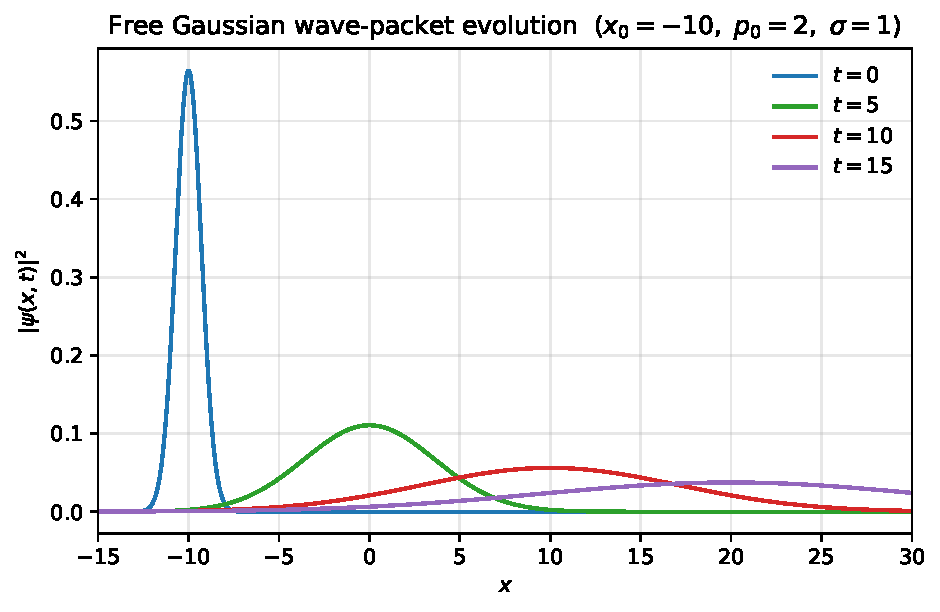
\includegraphics[width=0.9\linewidth]{ch00_wavepacket}
    \caption{$|\psi(x,t)|^{2}$ 在 $t=0,5,10,15$ 的快照. 波包中心严格沿 $\langle x\rangle_{t}=x_{0}+p_{0}t$ 平移, 同时高度下降、宽度增大——这就是``自由弥散''.}
    \label{fig:numexp-ch00}
\end{figure}
\begin{figure}[!htbp]
    \centering
    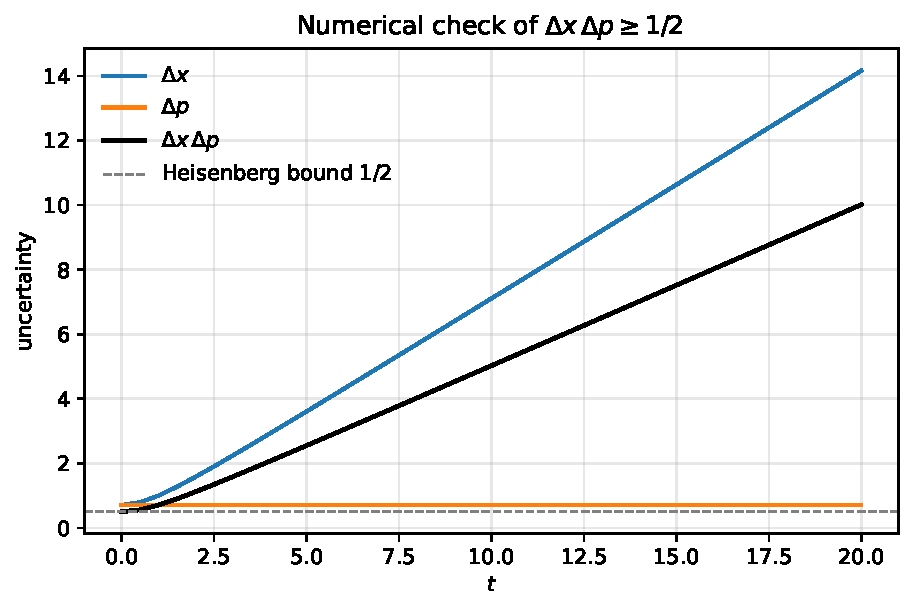
\includegraphics[width=0.75\linewidth]{ch00_uncertainty}
    \caption{$\Delta x(t)$, $\Delta p(t)$ 与乘积 $\Delta x\,\Delta p$ 随时间的变化. 灰色虚线为 Heisenberg 下界 $1/2$. 数值结果显示 $\Delta p$ 严格守恒 (因为 $[\Op H_{0},\Op p]=0$), $\Delta x$ 渐近线性增长, 乘积初值正好饱和 $1/2$ 后单调上升.}
    \label{fig:numexp-ch00-uncert}
\end{figure}

数值输出中前几行为
\begin{verbatim}
t =  0.00  <x> = -10.0000  Dx = 0.7071  <p> = +2.0000  Dp = 0.7071  DxDp = 0.5000
t =  5.00  <x> =  -0.0000  Dx = 3.6056  <p> = +2.0000  Dp = 0.7071  DxDp = 2.5495
t = 10.00  <x> = +10.0000  Dx = 7.1063  <p> = +2.0000  Dp = 0.7071  DxDp = 5.0249
t = 15.00  <x> = +20.0000  Dx = 10.6301  <p> = +2.0000  Dp = 0.7071  DxDp = 7.5166
\end{verbatim}
范数 $\|\psi_{t}\|^{2}$ 在所有时间点均为 $1.000000$, 与 $\Op U_{0}(t)$ 是幺正算符相符.

\subsection*{物理讨论}
\begin{itemize}
    \item \textbf{弥散公式的验证.} 对于初始相干态 Gauss 波包, 解析结果给出 $\Delta x(t)=\sigma\sqrt{1+t^{2}/\sigma^{4}}/\sqrt{2}$. 取 $\sigma=1$ 时, $\Delta x(t)=\sqrt{(1+t^{2})/2}$, 即 $t=0,5,10,15$ 处分别为 $0.7071,3.6056,7.1063,10.6301$, 与表中数值完全吻合, 直接验证了 \eqref{eq:qm-gauss-evolve}.
    \item \textbf{动量分布守恒.} $\Delta p$ 始终为 $1/\sqrt{2}\approx0.7071$. 这是因为 $|\widetilde\psi(p,t)|=|\widetilde\psi(p,0)|$, 自由演化只改变动量分量的相位, 不改变其模——这正是 $\hat\psi(\mathbf p)$ 在驻定相位法 \eqref{eq:qm-asymp-wave} 中保持不变的微观图像.
    \item \textbf{Heisenberg 饱和 \& 失饱和.} 初始 Gauss 是 $\Op x,\Op p$ 的极小不确定态, 故 $\Delta x\,\Delta p|_{t=0}=1/2$ 严格成立; 之后 $\Delta x$ 增大而 $\Delta p$ 不变, 乘积单调增大, 远离下界, 这与一般非定态下的 Robertson 不等式一致.
    \item \textbf{与 Riemann--Lebesgue 引理的呼应.} 图中可以看到, 在任意固定 $x$ 处, $|\psi(x,t)|^{2}$ 随时间趋于 $0$ (波包扫过后高度逐渐降低), 这正是 Riemann--Lebesgue 在弱意义下的体现: $\psi_{t}\rightharpoonup 0$, 但 $\|\psi_{t}\|=1$ 守恒, 故并不是强收敛——这是散射理论中区分 ``在/出态'' 与 ``渐近自由演化'' 的关键技术理由, 在第~\ref{sec:qm-review-summary} 节后续章节将反复用到.
\end{itemize}

\section{本章小结}\label{sec:qm-review-summary}

\begin{itemize}
    \item 散射是探索微观结构的关键工具, 从 Rutherford 到 LHC 都依赖它.
    \item 散射理论分为单道/多道、相对论/非相对论、时间相关/时间无关三对范畴; 本课程聚焦于非相对论、单道(随后会推广到多道)、并交替使用时间相关与时间无关两套语言.
    \item 量子态由 Hilbert 空间中的射线表示; 可观测量对应自伴算符. $L^{2}$ 与 $\ell^{2}$ 是两个具体而典型的可分 Hilbert 空间, 任意无穷维可分 Hilbert 空间都同构于 $\ell^{2}$.
    \item Dirac 记号通过 Riesz 引理把 Hilbert 空间与对偶空间一一联系起来; bra 是有界线性泛函, ket 是矢量.
    \item 线性算符可以是无界的, 因此一定要小心定义域. 厄米共轭对一般算符不一定 ``$A^{\dagger}=A$''; 自伴 (self-adjoint) 算符才有完整谱定理.
    \item 幺正算符要求 $\mathscr D=\mathscr R=\Hilb$, 等价于 $U^{\dagger}U=UU^{\dagger}=I$. Isometric 算符只要求 $\mathscr D=\Hilb$ 且保 norm; 在无穷维空间中, isometric $\not\Rightarrow$ unitary.
    \item 强极限与弱极限: 强极限是物理上有意义的``态相同'', 弱极限太弱; 散射理论中所有极限默认理解为强极限. 一系列幺正算符的强极限只能保证 isometric, 这正是 M\o ller 算符的来源.
    \item 自由演化算符 $\rme^{-\rmi\Op H_0 t/\hbar}$ 在动量空间是逐点相位 \eqref{eq:qm-U0-momentum}; 坐标空间的自由传播子 $K_{0}(\mathbf x,\mathbf x';t)$ 是 Gauss 振荡核 \eqref{eq:qm-free-propagator}, $|K_{0}|\propto|t|^{-3/2}$.
    \item 自由 Gauss 波包随时间线性弥散 \eqref{eq:qm-gauss-evolve}; 任意波包按 Riemann--Lebesgue 引理在每一固定坐标点弱收敛到零, 但范数守恒, 故无强极限.
    \item 驻定相位法给出长时间渐进 \eqref{eq:qm-asymp-wave}: 在 $\mathbf x=\mathbf v t$ 上, 波函数振幅 $\sim|t|^{-3/2}\hat\psi(m\mathbf v)$, 动量分布 $|\hat\psi(\mathbf p)|^{2}$ 守恒——这是 ``经典对应''与散射截面定义的物理依据.
    \item 自由 Green 算符 $\Op G_{0}(z)=(z-\Op H_{0})^{-1}$ 在动量空间为 \eqref{eq:qm-G0-p}, 在坐标空间是球面波 Green 函数 \eqref{eq:qm-G0-x}; $\pm\rmi 0^{+}$ 选择对应外向/内向边界条件, 这是 Lippmann--Schwinger 方程的种子.
\end{itemize}

掌握以上数学工具后, 我们就可以严格定义散射算符 $\Smat$ 与跃迁算符 $\Tmat$, 这是从第~\ref{ch:hilbert}~章 (Hilbert 空间与谱理论) 与第~\ref{ch:Smat1P}~章 (单粒子散射算符) 开始的内容.

\chapter{Hilbert 空间与谱理论 (Hilbert Space and Spectral Theory)}\label{ch:hilbert}

% --- local macros for this chapter ---
\providecommand{\N}{\mathbb{N}}
\providecommand{\Ker}{\operatorname{Ker}}

本章对量子散射理论所依赖的数学骨架——Hilbert 空间、自伴算符、谱定理与函数演算——做一次较为系统的整理. 第~\ref{ch:qmreview} 章已对 Hilbert 空间做了``物理风格''的回顾, Taylor 在《Scattering Theory》第一章亦只给出最简明的提要; 但是在散射理论中, 一旦我们要严格谈论 Møller 算符 $\Omega_{\pm}$ 的存在性 (见第~\ref{ch:Smat1P} 章)、强极限与幺正极限的区别、谱的分解 (绝对连续谱 ${\rm ac}$、纯点谱 ${\rm pp}$、奇异连续谱 ${\rm sc}$)、$\Op{H}$ 的函数演算 $f(\Op{H})$ (Green 算符 $(\Op{H}-z)^{-1}$ 即一例, 见第~\ref{ch:green} 章), 这些粗略的回顾就远远不够. 本章试图填补这一空缺.

行文上, 我们采取``物理学家的严格性''——重要定理给出准确的陈述并附带证明思路 (sketch), 读者可以参考 Reed--Simon 的四卷本或 Kato《Perturbation Theory for Linear Operators》获取完整证明. 主要参考: Taylor《Scattering Theory》第一章; Reed--Simon I, II, III; von Neumann《Mathematical Foundations of Quantum Mechanics》.

\section{Hilbert 空间的公理化定义}\label{sec:hilbert-axioms}

\subsection{内积空间}

\begin{definition}[内积空间 inner-product space]\label{def:hilbert-inner}
设 $V$ 是 $\C$ 上的线性空间. 一个 \emph{内积} (inner product) 是映射 $\inn{\cdot}{\cdot}:V\times V\to \C$ 满足:
\begin{enumerate}
    \item (共轭对称) $\inn{\psi}{\phi}=\overline{\inn{\phi}{\psi}}$;
    \item (第二变元线性) $\inn{\psi}{a\phi_1+b\phi_2}=a\,\inn{\psi}{\phi_1}+b\,\inn{\psi}{\phi_2}$, $a,b\in\C$;
    \item (正定) $\inn{\psi}{\psi}\geq 0$, 且 $\inn{\psi}{\psi}=0\Leftrightarrow\psi=0$.
\end{enumerate}
\end{definition}

我们采用物理学家约定: 内积对第一变元 \emph{反线性}, 对第二变元 \emph{线性}. 由内积出发可定义范数
\begin{equation}\label{eq:hilbert-norm}
\|\psi\|=\sqrt{\inn{\psi}{\psi}}.
\end{equation}

\begin{lemma}[Cauchy--Schwarz 不等式]\label{lem:hilbert-cs}
对任意 $\psi,\phi\in V$,
\begin{equation}\label{eq:hilbert-cs}
\bigl|\inn{\psi}{\phi}\bigr|\leq \|\psi\|\,\|\phi\|,
\end{equation}
等号成立当且仅当 $\psi,\phi$ 线性相关.
\end{lemma}

\begin{proof*}
若 $\phi=0$ 显然成立. 否则取 $\lambda=\inn{\phi}{\psi}/\|\phi\|^2$, 则 $0\leq \|\psi-\lambda\phi\|^2=\|\psi\|^2-|\inn{\phi}{\psi}|^2/\|\phi\|^2$, 整理得式 \eqref{eq:hilbert-cs}.
\end{proof*}

由 Cauchy--Schwarz 立刻得到三角不等式 $\|\psi+\phi\|\leq\|\psi\|+\|\phi\|$, 从而 $\|\cdot\|$ 是范数, $V$ 是赋范空间.

\subsection{完备性: 从内积空间到 Hilbert 空间}

完备性是 Hilbert 空间相对于一般内积空间的关键性质. 它保证了``Cauchy 列必收敛'', 从而可以谈论极限 (这正是散射理论需要的, 因为我们要让 $t\to\pm\infty$).

\begin{definition}[Cauchy 完备性]\label{def:hilbert-cauchy}
内积空间 $V$ 中的序列 $\{\psi_n\}$ 称为 \emph{Cauchy 列}, 若 $\forall\epsilon>0$, $\exists N$ 使 $m,n\geq N$ 时 $\|\psi_m-\psi_n\|<\epsilon$. 空间 $V$ \emph{完备}, 若每个 Cauchy 列都在 $V$ 中收敛 (即 $\exists\psi\in V$ s.t. $\|\psi_n-\psi\|\to 0$).
\end{definition}

\begin{definition}[Hilbert 空间]\label{def:hilbert-space}
\emph{Hilbert 空间} $\Hilb$ 是完备的复内积空间.
\end{definition}

\begin{definition}[可分性 separability]\label{def:hilbert-sep}
$\Hilb$ 称为 \emph{可分的} (separable), 若存在可数稠密子集 $\{\psi_n\}_{n=1}^{\infty}\subset\Hilb$.
\end{definition}

\begin{theorem}[可分 Hilbert 空间的标准正交基]\label{thm:hilbert-basis}
可分 Hilbert 空间 $\Hilb$ 必有可数标准正交基 (orthonormal basis) $\{e_n\}_{n\geq 1}$, 即 $\inn{e_m}{e_n}=\delta_{mn}$, 且每个 $\psi\in\Hilb$ 可展开为
\begin{equation}\label{eq:hilbert-expansion}
\psi=\sum_{n=1}^{\infty}\inn{e_n}{\psi}\,e_n,\qquad \|\psi\|^2=\sum_{n=1}^{\infty}|\inn{e_n}{\psi}|^2 \quad\text{(Parseval)}.
\end{equation}
\end{theorem}

\begin{remark}
量子力学只关心 \emph{可分的复 Hilbert 空间}. 一切实际系统的状态空间在适当的物理刻画下都是可分的 (例如自由度有限的多粒子系统是 $L^2$, 是可分的). Taylor《Scattering Theory》对此略而不谈, 但这是默认前提.
\end{remark}

\subsection{典型例子: \texorpdfstring{$L^2$}{L²} 与 \texorpdfstring{$\ell^2$}{ℓ²}}\label{subsec:hilbert-examples}

\begin{example}[$\ell^2(\N)$]\label{ex:hilbert-l2}
$\ell^2$ 是平方可和复序列空间:
\begin{equation}\label{eq:hilbert-ell2}
\ell^2=\Bigl\{(c_n)_{n\geq 1}\subset\C \mid \sum_{n=1}^{\infty}|c_n|^2<\infty\Bigr\},\quad \inn{c}{d}=\sum_{n=1}^{\infty}\overline{c_n}d_n.
\end{equation}
$\ell^2$ 是可分 Hilbert 空间, 标准基为 $e_n=(0,\ldots,0,1,0,\ldots)$.
\end{example}

\begin{example}[$L^2(\R^d)$]\label{ex:hilbert-L2}
$L^2(\R^d)$ 是 Lebesgue 平方可积函数 (在零测集等同) 空间:
\begin{equation}\label{eq:hilbert-L2}
L^2(\R^d)=\Bigl\{\psi:\R^d\to\C \text{ 可测} \mid \int_{\R^d}|\psi(\mathbf{x})|^2\,\rmd^d x<\infty\Bigr\},
\end{equation}
内积 $\inn{\psi}{\phi}=\int\overline{\psi(\mathbf{x})}\phi(\mathbf{x})\rmd^d x$. $L^2(\R^d)$ 是可分 Hilbert 空间; Hermite 函数 $\{h_{\mathbf{n}}\}_{\mathbf{n}\in\N_0^d}$ 给出一组标准基.
\end{example}

按照第 \ref{ch:qmreview} 章的物理记号, 单粒子无自旋态空间为 $\Hilb=L^2(\R^3)$; $N$ 个无自旋粒子取 $L^2(\R^{3N})$; 自旋 $s$ 单粒子取 $L^2(\R^3)\otimes\C^{2s+1}$.

\begin{theorem}[可分 Hilbert 空间唯一性]\label{thm:hilbert-unique}
任意两个无穷维可分 Hilbert 空间在等距同构 (unitary equivalence) 意义下唯一. 从而 $L^2(\R^d)\cong\ell^2(\N)$.
\end{theorem}

证明思路即取标准正交基 $\{e_n\}$, 则 $U:\psi\mapsto(\inn{e_n}{\psi})_n$ 是从 $\Hilb$ 到 $\ell^2$ 的幺正算符. 这告诉我们 $\Hilb$ 在抽象上只有一个; 但具体应用时, $L^2(\R^3)$ 的位置/动量表象是物理上自然的工具.

\subsection{对偶与 Riesz 表示}

\begin{theorem}[Riesz 表示定理]\label{thm:hilbert-riesz}
$\Hilb$ 上每个连续线性泛函 $\ell:\Hilb\to\C$ 必形如 $\ell(\psi)=\inn{\phi_\ell}{\psi}$, 其中 $\phi_\ell\in\Hilb$ 唯一.
\end{theorem}

Riesz 定理使得 Dirac 的 ``bra'' 记号有了严格意义: $\bra\phi\;\cdot\;\rangle$ 即是连续线性泛函 $\psi\mapsto\inn{\phi}{\psi}$. 但要小心: 像 $\bra{\mathbf{x}}$, $\bra{\mathbf{p}}$ 这种``反常基矢'' (improper kets/bras) 对应的不是 $\Hilb$ 中的元素 (它们不是平方可积的); 真正的严格框架需要 \emph{装备 Hilbert 空间} (rigged Hilbert space, Gelfand triple) $\Phi\subset\Hilb\subset\Phi'$, 见 Taylor 注脚 1-a-6 与第 \ref{ch:stationary} 章关于稳态散射态的讨论.

\section{算符的基本概念}\label{sec:hilbert-operators}

量子力学的可观测量、Hamilton 量、Møller 算符、$\Smat$ 矩阵无一例外都是 $\Hilb$ 上的线性算符. 然而很多重要算符 (如位置 $\Op{X}$、动量 $\Op{P}$、$\Op{H}=\Op{P}^2/2m+\Op{V}$) \emph{不是} 在整个 $\Hilb$ 上有定义的. 因此``算符的定义域'' (domain) 这件事必须严格对待.

\subsection{有界算符}

\begin{definition}[有界算符]\label{def:hilbert-bdd}
$A:\Hilb\to\Hilb$ 是 \emph{有界} (bounded) 的, 若 $\|A\|:=\sup_{\|\psi\|=1}\|A\psi\|<\infty$. 全体有界算符记 $\mathcal{B}(\Hilb)$.
\end{definition}

$\mathcal{B}(\Hilb)$ 在算子范数下是 Banach 代数. 散射算符 $\Smat$、Møller 算符 $\Omega_\pm$、时间演化 $\Op{U}(t)=\rme^{-\rmi\Op{H}t}$ 都是有界的甚至幺正的 (见第 \ref{ch:Smat1P} 章).

\subsection{无界算符与定义域}

许多物理上重要的算符是无界的. 一个具体例子见 Taylor 第 11 页:

\begin{example}[位置算符 $\Op{X}$ 在 $L^2(\R)$ 上]\label{ex:hilbert-position}
$(\Op{X}\psi)(x):=x\psi(x)$. 但若 $\psi\in L^2(\R)$, $\Op{X}\psi$ 不一定在 $L^2(\R)$. 实际上
\begin{equation}\label{eq:hilbert-domX}
\Dom(\Op{X})=\Bigl\{\psi\in L^2(\R)\mid\int x^2|\psi(x)|^2\rmd x<\infty\Bigr\}\subsetneq L^2(\R).
\end{equation}
取 $\psi(x)=(1+x^2)^{-1/2}/\sqrt{\pi}$ 则 $\psi\in L^2$, 但 $x\psi\notin L^2$. 故 $\Op{X}$ 是无界算符.
\end{example}

\begin{example}[动量算符 $\Op{P}=-\rmi\partial_x$]\label{ex:hilbert-momentum}
$\Op{P}$ 的``自然定义域'' Sobolev 空间 $H^1(\R)=\{\psi\in L^2(\R)\mid\hat\psi(p)\cdot p\in L^2\}$. 同样无界.
\end{example}

\begin{definition}[算符的图]\label{def:hilbert-graph}
算符 $A$ 的 \emph{图} (graph) 为 $\Gamma(A)=\{(\psi,A\psi)\mid\psi\in\Dom(A)\}\subset\Hilb\oplus\Hilb$.
\end{definition}

\begin{definition}[闭算符]\label{def:hilbert-closed}
$A$ 是 \emph{闭算符} (closed), 若 $\Gamma(A)$ 在 $\Hilb\oplus\Hilb$ (赋以图范数 $\|(\psi,\phi)\|^2=\|\psi\|^2+\|\phi\|^2$) 中是闭子集. 等价地: 若 $\psi_n\in\Dom(A)$, $\psi_n\to\psi$ 且 $A\psi_n\to\phi$, 则 $\psi\in\Dom(A)$ 且 $\phi=A\psi$.
\end{definition}

闭算符是无界算符理论中``可控'' 的对象——闭图定理 (closed graph theorem) 表明: 若 $A$ 闭且 $\Dom(A)=\Hilb$, 则 $A$ 有界. 由此, \emph{无界算符必定不能在整个 $\Hilb$ 上定义} (这正是 Taylor 注脚 1-c-7 想要警示的内容).

\begin{definition}[算符的扩张/限制]\label{def:hilbert-extension}
$B$ 是 $A$ 的 \emph{扩张}, 记 $A\subset B$, 若 $\Dom(A)\subset\Dom(B)$ 且 $A=B$ 在 $\Dom(A)$ 上.
\end{definition}

\begin{definition}[可闭算符]\label{def:hilbert-closable}
$A$ \emph{可闭}, 若它有闭扩张. 此时最小闭扩张 $\bar A$ 称为 $A$ 的 \emph{闭包} (closure).
\end{definition}

\subsection{值域、零空间}

记 $\Ran(A)=\{A\psi\mid\psi\in\Dom(A)\}$ (range), $\Ker(A)=\{\psi\in\Dom(A)\mid A\psi=0\}$. 则
\begin{equation}\label{eq:hilbert-range-ker}
\overline{\Ran(A)}=\Ker(A^\dagger)^{\perp},\qquad \Ker(A)=\overline{\Ran(A^\dagger)}^{\perp}
\end{equation}
(对闭稠定算符). 这是分析 Møller 算符值域 (\emph{渐近完备性} asymptotic completeness, 第 \ref{ch:Smat1P} 章) 的工具.

\section{伴随、对称、自伴}\label{sec:hilbert-adjoint}

\subsection{伴随算符}

\begin{definition}[稠定算符的伴随]\label{def:hilbert-adjoint}
设 $A$ 稠定 (即 $\Dom(A)$ 在 $\Hilb$ 中稠密). $A$ 的 \emph{伴随} $A^\dagger$ 由
\begin{align}
\Dom(A^\dagger)&=\{\phi\in\Hilb \mid \exists\eta\in\Hilb,\ \forall\psi\in\Dom(A),\ \inn{\phi}{A\psi}=\inn{\eta}{\psi}\},\notag\\
A^\dagger\phi&:=\eta. \label{eq:hilbert-adjoint-def}
\end{align}
$\Dom(A)$ 稠密保证 $\eta$ 唯一. $A^\dagger$ 始终是闭算符.
\end{definition}

\begin{definition}[对称、自伴、本质自伴]\label{def:hilbert-sym-sa}
设 $A$ 稠定. 称
\begin{itemize}
    \item $A$ \emph{对称} (symmetric, ``Hermitian''), 若 $A\subset A^\dagger$, 即 $\inn{\phi}{A\psi}=\inn{A\phi}{\psi}$ 对 $\phi,\psi\in\Dom(A)$ 成立;
    \item $A$ \emph{自伴} (self-adjoint), 若 $A=A^\dagger$ (作为算符的相等, 包含 $\Dom(A)=\Dom(A^\dagger)$);
    \item $A$ \emph{本质自伴} (essentially self-adjoint), 若 $A$ 对称且其闭包 $\bar A$ 是自伴.
\end{itemize}
\end{definition}

物理学家几乎不区分 ``Hermitian'' 与 ``self-adjoint''; 但数学上自伴比对称严格得多. 例如 $\Op{P}=-\rmi\partial_x$ 在 $C_c^\infty([0,1])$ 上对称却不自伴: 改变 $\Dom$ 的边界条件 (周期边界 vs. Dirichlet) 给出不同的自伴扩张.

\begin{remark}
量子力学中 \emph{可观测量必须是自伴算符}, 而不仅仅是对称算符. 这是 von Neumann 的洞察, Taylor 在第 8 页的注脚里也指出 ``self-adjointness is the stronger property''. 自伴而非对称才能保证有谱定理, 才能定义函数演算 $f(A)$, 才能保证 $\rme^{-\rmi A t}$ 是良好定义的幺正群 (见 Stone 定理).
\end{remark}

\subsection{亏指数判据 (von Neumann)}

如何判断对称算符是否本质自伴? Hilbert 空间理论的核心结果之一:

\begin{theorem}[von Neumann 亏指数判据]\label{thm:hilbert-deficiency}
设 $A$ 闭对称, 定义 \emph{亏空间} (deficiency subspaces)
\begin{equation}\label{eq:hilbert-defspaces}
\mathcal{K}_{\pm}=\Ker(A^\dagger\mp \rmi)=\Ran(A\pm \rmi)^{\perp},
\end{equation}
和 \emph{亏指数} (deficiency indices) $n_{\pm}=\dim\mathcal{K}_{\pm}$. 则:
\begin{enumerate}
    \item $A$ 自伴 $\iff$ $n_+=n_-=0$;
    \item $A$ 有自伴扩张 $\iff$ $n_+=n_-$ (这时扩张的集合与 $\mathcal{K}_+\to\mathcal{K}_-$ 的幺正映射一一对应);
    \item $n_+\neq n_-$: 没有自伴扩张.
\end{enumerate}
\end{theorem}

\begin{proof*}[证明思路]
要判断对称算符 $A$ 是否自伴, 即看 $A$ 与 $A^\dagger$ 是否吻合. 关键观察: $A^\dagger$ 自动是闭的, 且
\begin{equation*}
\Dom(A^\dagger)=\Dom(\bar A)\dotplus\mathcal{K}_+\dotplus\mathcal{K}_-,\quad \text{(直和)}
\end{equation*}
这是 von Neumann 的``一阶分解''. 因此 $\bar A=A^\dagger$ 当且仅当 $\mathcal{K}_+=\mathcal{K}_-=\{0\}$. 自伴扩张则对应于在 $\mathcal{K}_+\oplus\mathcal{K}_-$ 中选 ``Cayley 变换''$U:\mathcal{K}_+\to\mathcal{K}_-$, 这要求 $\dim\mathcal{K}_+=\dim\mathcal{K}_-$. 详细见 Reed--Simon II, Thm. X.1.
\end{proof*}

\subsection{标准反例: 半直线动量算符}\label{subsec:hilbert-counterex}

\begin{example}[$\Op{P}=-\rmi\partial_x$ 在 $L^2([0,\infty))$]\label{ex:hilbert-halfline}
取 $\Dom(A)=C_c^\infty((0,\infty))$. 容易验证 $A$ 对称. 计算亏空间: $A^\dagger\phi=\rmi\phi$ 即 $-\rmi\phi'=\rmi\phi$, $\phi(x)=c\rme^{-x}\in L^2([0,\infty))$. 所以 $n_+=1$. 类似 $A^\dagger\phi=-\rmi\phi$ 给 $\phi(x)=c\rme^x\notin L^2$, 故 $n_-=0$. 故 $n_+\neq n_-$, $A$ \textbf{不可能}有自伴扩张! 这是经典反例: 半直线上的``动量算符''并不存在自伴版本——直观上, 边界 $x=0$ 上 ``概率流'' 只能流出, 不能进出对称, 故无法保持厄米性.
\end{example}

\begin{example}[{$\Op{P}=-\rmi\partial_x$ 在 $L^2([0,1])$}]
亏指数 $n_\pm=1$, 自伴扩张构成 $U(1)$ 族, 对应边界条件 $\psi(1)=\rme^{\rmi\theta}\psi(0)$, $\theta\in[0,2\pi)$. 物理上即不同的相位边界条件.
\end{example}

\subsection{Kato--Rellich 定理}\label{subsec:hilbert-kato}

散射理论中通常 $\Op{H}=\Op{H}_0+\Op{V}$, $\Op{H}_0=\Op{P}^2/2m$. 自伴性的标准工具:

\begin{theorem}[Kato--Rellich]\label{thm:hilbert-kato}
设 $\Op{H}_0$ 自伴, $\Op{V}$ 对称且 $\Op{H}_0$-有界 (即 $\Dom(\Op{H}_0)\subset\Dom(\Op{V})$ 且存在 $a<1$, $b\geq 0$ 使
\begin{equation}\label{eq:hilbert-katobound}
\|\Op{V}\psi\|\leq a\|\Op{H}_0\psi\|+b\|\psi\|,\quad \psi\in\Dom(\Op{H}_0)).
\end{equation}
则 $\Op{H}_0+\Op{V}$ 在 $\Dom(\Op{H}_0)$ 上自伴.
\end{theorem}

例如, 对于 Coulomb 势 $V=-Ze^2/r$ 在 $L^2(\R^3)$ 上, $\Op{V}$ 是 $\Op{H}_0=-\nabla^2/2m$-有界的 (Kato 不等式 $\|r^{-1}\psi\|\leq 2\|\nabla\psi\|$), 故 $\Op{H}=\Op{H}_0-Ze^2/r$ 自伴, 这正是氢原子 Hamilton 量自伴的证明 (见第 \ref{ch:qmreview} 章).

\section{谱与预解集}\label{sec:hilbert-spectrum}

\subsection{预解算符}

\begin{definition}[谱、预解集]\label{def:hilbert-spectrum}
设 $A$ 闭. \emph{预解集} (resolvent set)
\begin{equation}\label{eq:hilbert-resolventset}
\rho(A)=\{z\in\C\mid A-z:\Dom(A)\to\Hilb\text{ 双射}, (A-z)^{-1}\in\mathcal{B}(\Hilb)\}.
\end{equation}
对 $z\in\rho(A)$, $R(z;A):=(A-z)^{-1}$ 是 \emph{预解算符} (resolvent). \emph{谱} (spectrum) $\sigma(A)=\C\setminus\rho(A)$.
\end{definition}

预解算符 $R(z;A)$ 在物理上即 \emph{Green 算符} (见第 \ref{ch:green} 章). $\rho(A)$ 是开集, $z\mapsto R(z;A)$ 在 $\rho(A)$ 上解析 (operator-valued analytic), 且
\begin{equation}\label{eq:hilbert-resolvent-id}
R(z;A)-R(w;A)=(z-w)R(z;A)R(w;A)\quad \text{(第一预解恒等式)}.
\end{equation}

\subsection{谱的分类}

\begin{definition}[谱的细分]\label{def:hilbert-spec-decomp}
$\sigma(A)$ 划分为三个互不相交的子集:
\begin{itemize}
    \item \emph{点谱} (point spectrum) $\sigma_p(A)=\{\lambda\mid\Ker(A-\lambda)\neq\{0\}\}$, 即 \emph{本征值}集合;
    \item \emph{连续谱} (continuous spectrum) $\sigma_c(A)=\{\lambda\notin\sigma_p\mid\overline{\Ran(A-\lambda)}=\Hilb,\ (A-\lambda)^{-1}\text{ 无界}\}$;
    \item \emph{剩余谱} (residual spectrum) $\sigma_r(A)=\{\lambda\notin\sigma_p\mid\overline{\Ran(A-\lambda)}\neq\Hilb\}$.
\end{itemize}
\end{definition}

\begin{theorem}\label{thm:hilbert-sa-spec}
若 $A$ 自伴, 则:
\begin{enumerate}
    \item $\sigma(A)\subset\R$;
    \item $\sigma_r(A)=\emptyset$ (自伴算符无剩余谱);
    \item $\|R(z;A)\|\leq |\Im z|^{-1}$ for $\Im z\neq 0$.
\end{enumerate}
\end{theorem}

\begin{proof*}[(2) 的证明]
若 $\lambda\in\sigma_r(A)$, 则 $\overline{\Ran(A-\lambda)}\neq\Hilb$, 故 $\exists\, 0\neq\eta\perp\Ran(A-\lambda)$. 由 \eqref{eq:hilbert-range-ker}, $\eta\in\Ker(A^\dagger-\bar\lambda)=\Ker(A-\bar\lambda)$ (因为 $A$ 自伴且 $\sigma\subset\R$, $\bar\lambda=\lambda$). 故 $\lambda\in\sigma_p$, 矛盾.
\end{proof*}

\subsection{谱映射定理 (基本版)}

\begin{theorem}[多项式谱映射]\label{thm:hilbert-spec-mapping}
设 $A$ 有界, $p\in\C[z]$. 则 $\sigma(p(A))=p(\sigma(A))$.
\end{theorem}

更一般的谱映射涉及连续函数演算, 见下节. 例如对 $\Op{H}\geq 0$ 自伴有 $\sigma(\Op{H}^2)=\sigma(\Op{H})^2$.

\section{谱定理 (自伴算符)}\label{sec:hilbert-spectral-thm}

谱定理是 Hilbert 空间理论的顶峰. 对自伴算符, 有三种等价形式: (i) 投影测度 (projection-valued measure, PVM) 形式; (ii) 乘法算符形式; (iii) 函数演算形式. 我们陈述前两种, 并简述思路.

\subsection{投影测度形式}

\begin{definition}[投影值测度 PVM]\label{def:hilbert-pvm}
\emph{投影值测度} 是映射 $E:\mathcal{B}(\R)\to\mathcal{B}(\Hilb)$ ($\mathcal{B}(\R)$ 为 Borel $\sigma$-代数) 满足
\begin{enumerate}
    \item $E(\Omega)$ 是正交投影 ($E(\Omega)^2=E(\Omega)=E(\Omega)^\dagger$) 对每个 Borel 集 $\Omega\subset\R$;
    \item $E(\emptyset)=0,\ E(\R)=\Op{1}$;
    \item $E(\Omega_1\cap\Omega_2)=E(\Omega_1)E(\Omega_2)$;
    \item ($\sigma$-可加) 若 $\{\Omega_n\}$ 互不相交, $E(\cup_n\Omega_n)=\sum_n E(\Omega_n)$ 强收敛.
\end{enumerate}
对每个 $\psi\in\Hilb$, $\mu_\psi(\Omega):=\inn{\psi}{E(\Omega)\psi}=\|E(\Omega)\psi\|^2$ 是 $\R$ 上的有限正测度 (\emph{谱测度} spectral measure).
\end{definition}

\begin{theorem}[谱定理 -- PVM 形式]\label{thm:hilbert-spec-pvm}
设 $A$ 是 $\Hilb$ 上自伴算符. 存在 \emph{唯一} 的 PVM $E_A$ on $\R$ 使得
\begin{equation}\label{eq:hilbert-spec-thm-pvm}
A=\int_{\R}\lambda\,\rmd E_A(\lambda),\qquad \Dom(A)=\Bigl\{\psi\mid\int_\R \lambda^2\,\rmd\mu_\psi(\lambda)<\infty\Bigr\}.
\end{equation}
此外 $\sigma(A)={\rm supp}(E_A)=\{\lambda\in\R\mid E_A((\lambda-\epsilon,\lambda+\epsilon))\neq 0\,\forall\epsilon>0\}$.
\end{theorem}

物理上, $E_A((-\infty,\lambda])$ 即 ``$A\leq\lambda$ 的事件投影''; 谱测度 $\mu_\psi$ 即测量 $A$ 时取值 $\leq\lambda$ 的概率分布 $F_\psi(\lambda)=\|E_A((-\infty,\lambda])\psi\|^2$, 这就是 \emph{谱分解} 的物理意义.

\subsection{乘法算符形式}

\begin{theorem}[谱定理 -- 乘法算符形式]\label{thm:hilbert-spec-mult}
设 $A$ 自伴. 存在测度空间 $(M,\mu)$ ($\mu$ $\sigma$-有限), 实值可测函数 $f:M\to\R$, 与幺正映射 $U:\Hilb\to L^2(M,\mu)$ 使
\begin{equation}\label{eq:hilbert-spec-thm-mult}
(UAU^{-1}\tilde\psi)(m)=f(m)\tilde\psi(m),
\end{equation}
即 $A$ 通过 $U$ 同构于 $L^2(M,\mu)$ 上的 \emph{乘 $f$} 算符. $\Dom(UAU^{-1})=\{\tilde\psi\mid f\tilde\psi\in L^2\}$.
\end{theorem}

直观地: \emph{所有自伴算符``在适当表象下都是位置算符''}. 这是 Dirac/$\delta$-基矢的严格化.

\subsection{证明思路 (sketch)}

证明谱定理通常分两步:

\textbf{第一步: 有界自伴算符的连续函数演算.} 由多项式谱映射 \ref{thm:hilbert-spec-mapping}, 对 $A$ 有界自伴有 $\|p(A)\|=\sup_{\lambda\in\sigma(A)}|p(\lambda)|$. 由 Stone--Weierstrass, $p\mapsto p(A)$ 可延拓为 $C^*$-同态 $C(\sigma(A))\to\mathcal{B}(\Hilb)$, $f\mapsto f(A)$. 这是 \emph{连续函数演算}.

\textbf{第二步: 由 Riesz--Markov 构造谱测度.} 对每个 $\psi$, $f\mapsto \inn{\psi}{f(A)\psi}$ 是 $C(\sigma(A))$ 上的正泛函, 由 Riesz--Markov 给出 Borel 测度 $\mu_\psi$. 极化得到 $\mu_{\psi,\phi}$. 由此 $\inn{\psi}{f(A)\phi}=\int f\,\rmd\mu_{\psi,\phi}$ 对 \emph{Borel 函数}延拓, 即得 PVM.

\textbf{第三步: 无界算符的情形.} 通过 Cayley 变换 $U=(A-\rmi)(A+\rmi)^{-1}$ 把无界自伴 $A$ 化为幺正 (有界) 算符 $U$, 应用有界版本于 $U$, 然后逆变换. 见 Reed--Simon I, Thm. VIII.6.

\subsection{对易自伴算符族的联合谱测度}

\begin{theorem}[多个对易自伴算符]\label{thm:hilbert-joint-spec}
设 $A_1,\ldots,A_n$ 自伴且预解算符两两对易. 存在 $\R^n$ 上的联合 PVM $E$ 使
\begin{equation}
A_k=\int_{\R^n}\lambda_k\,\rmd E(\lambda_1,\ldots,\lambda_n).
\end{equation}
\end{theorem}

物理意义: 一组完备对易可观测量 (CSCO) 给出 $\Hilb$ 在它们公共本征值上的``连续基矢''. 例如 $\{\Op{X}_1,\Op{X}_2,\Op{X}_3\}$ 在 $L^2(\R^3)$ 上的联合 PVM 即位置表象.

\section{函数演算}\label{sec:hilbert-functional-calc}

\subsection{Borel 函数演算}

由谱定理我们可以对 \emph{任何 Borel 可测} 函数 $f:\R\to\C$ 定义
\begin{empheq}[box=\fbox]{equation}\label{eq:hilbert-fcalc}
f(A)=\int_{\R}f(\lambda)\,\rmd E_A(\lambda),
\end{empheq}
$\Dom(f(A))=\{\psi\mid\int |f(\lambda)|^2\rmd\mu_\psi<\infty\}$. 性质:
\begin{itemize}
    \item $(fg)(A)=f(A)g(A)$, $\overline{f(A)}\subset \bar f(A)$;
    \item $f$ 实值 $\Rightarrow$ $f(A)$ 自伴;
    \item $|f|=1$ $\Rightarrow$ $f(A)$ 幺正;
    \item $f\geq 0$ $\Rightarrow$ $f(A)\geq 0$;
    \item 谱映射 $\sigma(f(A))=\overline{f(\sigma(A))}$ (对 $f$ 连续).
\end{itemize}

物理示例:
\begin{itemize}
    \item $\Op{U}(t)=\rme^{-\rmi\Op{H}t}=\int \rme^{-\rmi\lambda t}\rmd E_{\Op{H}}(\lambda)$: 时间演化 (见 \S\ref{sec:hilbert-stone});
    \item $R(z;\Op{H})=(\Op{H}-z)^{-1}=\int(\lambda-z)^{-1}\rmd E_{\Op{H}}(\lambda)$: Green 算符 (见第 \ref{ch:green} 章);
    \item $\Op{H}^{1/2}$ ($\Op{H}\geq 0$): 平方根; 用于动量空间 $|\mathbf{p}|=\sqrt{\Op{P}^2}$ 的相对论分散.
\end{itemize}

\subsection{Borel 函数演算的连续性}

\begin{proposition}\label{prop:hilbert-fcalc-cont}
设 $f_n\to f$ 逐点 (Borel 可测) 且 $|f_n|\leq M$ (一致). 则 $f_n(A)\to f(A)$ 强收敛, 即 $f_n(A)\psi\to f(A)\psi$ 对每个 $\psi\in\Hilb$.
\end{proposition}

这一``强收敛''而非``一致''将在第 \ref{ch:Smat1P} 章 Møller 算符存在性中起决定作用.

\section{Stone 定理与单参数幺正群}\label{sec:hilbert-stone}

量子力学的核心方程 Schrödinger 方程
\begin{equation}\label{eq:hilbert-schroedinger}
\rmi\frac{\rmd}{\rmd t}\ket{\psi_t}=\Op{H}\ket{\psi_t}
\end{equation}
其解 $\ket{\psi_t}=\Op{U}(t)\ket{\psi_0}$, $\Op{U}(t)=\rme^{-\rmi\Op{H}t}$, 是一个 \emph{强连续单参数幺正群}.

\begin{definition}[强连续单参数幺正群]\label{def:hilbert-spgroup}
$\{U(t)\}_{t\in\R}$ 是 \emph{强连续单参数幺正群} (one-parameter unitary group), 若
\begin{enumerate}
    \item 每个 $U(t)$ 是 $\Hilb$ 上幺正算符;
    \item $U(s+t)=U(s)U(t)$, $U(0)=\Op{1}$;
    \item $t\mapsto U(t)\psi$ 对每个 $\psi\in\Hilb$ 强连续.
\end{enumerate}
\end{definition}

\begin{theorem}[Stone 定理]\label{thm:hilbert-stone}
$\{U(t)\}$ 与 $\Hilb$ 上自伴算符 $A$ 一一对应, 关系为
\begin{equation}\label{eq:hilbert-stone}
U(t)=\rme^{-\rmi A t},\qquad A\psi=\rmi\frac{\rmd}{\rmd t}\Big|_{t=0}U(t)\psi,\quad \psi\in\Dom(A),
\end{equation}
其中 $\Dom(A)=\{\psi\mid \lim_{t\to 0}t^{-1}(U(t)\psi-\psi)\text{ 存在}\}$ (称 \emph{无穷小生成元}).
\end{theorem}

证明思路: ($\Leftarrow$) 由谱定理直接定义 $U(t)=\int \rme^{-\rmi\lambda t}\rmd E_A(\lambda)$, 验证三条性质. ($\Rightarrow$) 给定 $U$, 形式定义 $A=\rmi U'(0)$, 关键技术是用积分 $\int_0^t U(s)\psi\,\rmd s$ 构造 $\Dom(A)$ 中的稠密子集 (Gårding 域), 然后扩张. 见 Reed--Simon I, Thm. VIII.7.

\begin{remark}[Stone 定理的物理意义]
Stone 定理说明自伴 $\Op{H}$ 与酉时间演化 $\rme^{-\rmi\Op{H}t}$ 是同一物理事实的两种描述. 自伴性是\emph{概率守恒} ($\|\Op{U}(t)\psi\|=\|\psi\|$) 的数学等价物.

特别地, 散射问题中我们将比较两组演化:
\begin{equation}\label{eq:hilbert-twoevolutions}
\Op{U}_0(t)=\rme^{-\rmi\Op{H}_0 t},\qquad \Op{U}(t)=\rme^{-\rmi\Op{H} t},
\end{equation}
其中 $\Op{H}=\Op{H}_0+\Op{V}$. Møller 算符
\begin{equation}\label{eq:hilbert-moller}
\Omega_\pm=\lim_{t\to\mp\infty}\Op{U}(t)^\dagger\,\Op{U}_0(t),
\end{equation}
正是 Stone 定理保证的两个幺正群的``渐近比较''. 它们的存在性、值域、完备性是第 \ref{ch:Smat1P} 章的核心.
\end{remark}

\section{谱的细分: 纯点 / 绝对连续 / 奇异连续}\label{sec:hilbert-spec-decomp-fine}

$\sigma(A)$ 的``点谱/连续谱/剩余谱''分类对自伴算符并不够细. 散射理论中真正有用的是 \emph{Lebesgue 分解}.

\subsection{谱测度的 Lebesgue 分解}

任意 $\R$ 上 Borel 测度 $\mu$ 有 \emph{唯一}的 Lebesgue 分解
\begin{equation}\label{eq:hilbert-lebesgue}
\mu=\mu_{\rm pp}+\mu_{\rm ac}+\mu_{\rm sc},
\end{equation}
其中 $\mu_{\rm pp}$ 集中在可数集 (\emph{纯点}); $\mu_{\rm ac}\ll\rmd\lambda$ (\emph{绝对连续}, 关于 Lebesgue 测度); $\mu_{\rm sc}$ \emph{奇异连续} (集中在 Lebesgue 零测集但无原子, 例 Cantor 测度).

\subsection{$\Hilb$ 的谱分解}

\begin{definition}[谱子空间]\label{def:hilbert-spec-subsp}
对自伴 $A$, 定义
\begin{equation}\label{eq:hilbert-spec-subspaces}
\Hilb_{\bullet}(A):=\{\psi\in\Hilb\mid \mu_\psi^A\text{ 是 } \bullet\text{-型}\},\quad \bullet\in\{{\rm pp},{\rm ac},{\rm sc}\}.
\end{equation}
则
\begin{equation}\label{eq:hilbert-spec-decomp-H}
\Hilb=\Hilb_{\rm pp}(A)\oplus\Hilb_{\rm ac}(A)\oplus\Hilb_{\rm sc}(A),
\end{equation}
每个子空间 $A$-不变.
\end{definition}

定义 $\sigma_{\rm pp}(A), \sigma_{\rm ac}(A), \sigma_{\rm sc}(A)$ 为 $A$ 限制在相应子空间上的谱.

\begin{itemize}
    \item $\Hilb_{\rm pp}(A)$ 由 $A$ 的本征向量张成. \emph{束缚态} (bound states) 都在这里.
    \item $\Hilb_{\rm ac}(A)$ 是\emph{散射态} (scattering states) 的天然位置: 从这里出发的态在能量 (即 $A=\Op{H}$ 时) 上``连续''分布, 满足 RAGE 类的``逃逸到无穷''性质.
    \item $\Hilb_{\rm sc}(A)$ 是奇异连续部分. 物理上``反常'', 出现于 fractal 势/拟周期 Schrödinger 算符等. 短程势 + Coulomb 修正下通常 $\Hilb_{\rm sc}=\{0\}$.
\end{itemize}

\subsection{RAGE 定理}

谱分解的物理意义由 Ruelle--Amrein--Georgescu--Enss (RAGE) 定理刻画:

\begin{theorem}[RAGE 定理 (粗略版)]\label{thm:hilbert-rage}
设 $\Op{H}$ 自伴, $C$ 紧算符. 则:
\begin{enumerate}
    \item 对 $\psi\in\Hilb_{\rm pp}(\Op{H})$,
    \begin{equation}\label{eq:hilbert-rage-pp}
    \sup_{t\in\R}\|C\rme^{-\rmi\Op{H}t}\psi\|<\infty,
    \end{equation}
    甚至 $C\rme^{-\rmi\Op{H}t}\psi$ 是 $\R$ 上的 (近) 周期函数;
    \item 对 $\psi\in\Hilb_{\rm c}(\Op{H})=\Hilb_{\rm ac}\oplus\Hilb_{\rm sc}$,
    \begin{equation}\label{eq:hilbert-rage-c}
    \frac{1}{T}\int_0^T \|C\rme^{-\rmi\Op{H}t}\psi\|^2\,\rmd t \xrightarrow[T\to\infty]{} 0;
    \end{equation}
    \item 对 $\psi\in\Hilb_{\rm ac}(\Op{H})$, 上式的时间平均加强为
    \begin{equation}\label{eq:hilbert-rage-ac}
    \|C\rme^{-\rmi\Op{H}t}\psi\|\xrightarrow[t\to\pm\infty]{}0.
    \end{equation}
\end{enumerate}
\end{theorem}

物理解释: 取 $C=\chi_{|\mathbf{x}|<R}$ (空间紧支撑特征函数, 是紧算符当 $\Op{H}=-\nabla^2/2m$). 则
\begin{itemize}
    \item 束缚态 ($\Hilb_{\rm pp}$) 一直留在有限区域内: $\|\chi_{|\mathbf{x}|<R}\rme^{-\rmi\Op{H}t}\psi\|^2\to\|\psi\|^2$ 在 $R$ 大时;
    \item 散射态 ($\Hilb_{\rm ac}$) 在 $|t|\to\infty$ 时跑到无穷远: $\|\chi_{|\mathbf{x}|<R}\rme^{-\rmi\Op{H}t}\psi\|\to 0$.
\end{itemize}

这就是``束缚态/散射态''的精确数学定义. Taylor 第 10 页朴素地写下 $\Hilb=\mathcal{R}\oplus\mathcal{B}$ (scattering ${\oplus}$ bound), 严格的版本即 $\mathcal{B}=\Hilb_{\rm pp}(\Op{H})$, $\mathcal{R}=\Hilb_{\rm ac}(\Op{H})$ (假设 $\Hilb_{\rm sc}=0$). \emph{渐近完备性} (asymptotic completeness) 的真正陈述就是
\begin{equation}\label{eq:hilbert-asymptcomp}
\Ran\Omega_+=\Ran\Omega_-=\Hilb_{\rm ac}(\Op{H})\quad (\text{且 }\Hilb_{\rm sc}(\Op{H})=\{0\}).
\end{equation}
详见第 \ref{ch:Smat1P} 章.

\section{算符的收敛模式}\label{sec:hilbert-conv}

散射理论与 Møller 算符的存在性问题, 关键在于不同收敛模式间的差别. Taylor \S 1-f, 1-g 已对此作了物理风味讨论, 这里给出严格的对比.

\subsection{三种收敛}

\begin{definition}[范数 / 强 / 弱收敛]\label{def:hilbert-conv}
设 $\{A_n\}\subset\mathcal{B}(\Hilb)$, $A\in\mathcal{B}(\Hilb)$.
\begin{itemize}
    \item \emph{范数收敛} (norm / uniform): $\|A_n-A\|\to 0$, 记 $A_n\xrightarrow{\|\cdot\|}A$.
    \item \emph{强收敛} (strong): $\|A_n\psi-A\psi\|\to 0$ 对每个 $\psi\in\Hilb$, 记 $A_n\xrightarrow{s}A$.
    \item \emph{弱收敛} (weak): $\inn{\phi}{A_n\psi}\to\inn{\phi}{A\psi}$ 对每对 $\phi,\psi\in\Hilb$, 记 $A_n\xrightarrow{w}A$.
\end{itemize}
\end{definition}

\begin{theorem}[蕴含关系]\label{thm:hilbert-conv-impl}
范数收敛 $\Rightarrow$ 强收敛 $\Rightarrow$ 弱收敛, 反向蕴含一般 \emph{不成立}.
\end{theorem}

类似地对态矢: 强 $\|\psi_n-\psi\|\to 0$ vs.\ 弱 $\inn{\phi}{\psi_n}\to\inn{\phi}{\psi}$ 对所有 $\phi$.

\subsection{反例: 反向蕴含失败}

Taylor 第 18 页就已给出强收敛不蕴含范数收敛的关键例子:

\begin{example}[自由波包 -- 弱不强]\label{ex:hilbert-freewavepacket}
$\ket{\psi_t}=\rme^{-\rmi\Op{H}_0 t}\ket{\psi_0}$, $\Op{H}_0=\Op{P}^2/2m$. 则对每个固定 $\ket{\phi}\in L^2(\R^3)$,
\begin{equation}\label{eq:hilbert-freedisp}
\inn{\phi}{\psi_t}\xrightarrow{|t|\to\infty} 0,
\end{equation}
但 $\|\psi_t\|=\|\psi_0\|=1$ 不变. 即 $\ket{\psi_t}\xrightarrow{w}0$ 而 \emph{不}强收敛到 $0$. 物理解释: 自由波包不断弥散, 在任意有限区域 (代表 $\ket\phi$) 中的概率趋零.

证明思路: 取 $\ket\phi$ 为 Gauss 包, 显式计算 $\inn{\phi}{\psi_t}$ 利用稳相法得 $|\inn{\phi}{\psi_t}|\sim t^{-3/2}$. 一般情形由 Gauss 函数稠密性逼近.
\end{example}

\begin{example}[等距非幺正算符 (Taylor \S 1-e)]\label{ex:hilbert-isometric}
取 $\ell^2$ 上 \emph{右移算符} $\Omega:e_n\mapsto e_{n+1}$. 则 $\Omega$ 等距 ($\Omega^\dagger\Omega=\Op{1}$) 但 \emph{不}幺正 ($\Omega\Omega^\dagger=\Op{1}-|e_1\rangle\langle e_1|$). 这正是 Taylor 第 14--15 页指出的``等距 $\not\Rightarrow$ 幺正''. 物理上: Møller 算符 $\Omega_\pm$ 在不存在束缚态的特殊情形是幺正; 一般情形仅是等距 (其值域是 $\Hilb_{\rm ac}(\Op{H})\subsetneq\Hilb$).
\end{example}

\subsection{乘积的连续性}

\begin{proposition}\label{prop:hilbert-product-cont}
设 $A_n\xrightarrow{s}A$, $B_n\xrightarrow{s}B$, 且 $\sup_n\|A_n\|<\infty$. 则 $A_nB_n\xrightarrow{s}AB$.

但: $A_n\xrightarrow{w}A$ 与 $B_n\xrightarrow{w}B$ 一般 \emph{不蕴含} $A_nB_n\xrightarrow{w}AB$.
\end{proposition}

\begin{proof*}[(强情形)]
$\|A_nB_n\psi-AB\psi\|\leq\|A_n\|\|B_n\psi-B\psi\|+\|(A_n-A)B\psi\|\to 0$.
\end{proof*}

\begin{proposition}\label{prop:hilbert-adjoint-noncont}
$A_n\xrightarrow{s}A$ \emph{不蕴含} $A_n^\dagger\xrightarrow{s}A^\dagger$ (但 $\xrightarrow{w}$ 蕴含 $\xrightarrow{w}$).
\end{proposition}

Taylor \S 1-g 末段对此评论: ``If $A_t\to A$ it is not necessarily true that $A_t^\dagger\to A^\dagger$.'' 这正是 Møller 算符存在但 \emph{逆} 不存在的根源.

\subsection{应用于 Møller 算符}

定义
\begin{equation}\label{eq:hilbert-moller-strong}
\Omega_\pm\psi:=\lim_{t\to\mp\infty}\rme^{\rmi\Op{H}t}\rme^{-\rmi\Op{H}_0 t}\psi.
\end{equation}
极限取 \emph{强意义}. Cook 判据给出充分条件:

\begin{theorem}[Cook 判据]\label{thm:hilbert-cook}
若存在 $\psi_0\in\Dom(\Op{H})\cap\Dom(\Op{H}_0)$ 的稠密子集, 使
\begin{equation}\label{eq:hilbert-cook}
\int_{0}^{\infty}\|\Op{V}\rme^{-\rmi\Op{H}_0 t}\psi_0\|\,\rmd t<\infty,
\end{equation}
则强极限 $\Omega_-$ 在 $\psi_0$ 上存在 (对 $\Omega_+$ 相应地积分 $\int_{-\infty}^0$).
\end{theorem}

\begin{proof*}[思路]
利用 Stone 定理与基本定理:
\begin{equation*}
\rme^{\rmi\Op{H}t}\rme^{-\rmi\Op{H}_0 t}\psi_0-\psi_0
=\rmi\int_0^t\rme^{\rmi\Op{H}s}\Op{V}\rme^{-\rmi\Op{H}_0 s}\psi_0\,\rmd s.
\end{equation*}
被积式范数 $=\|\Op{V}\rme^{-\rmi\Op{H}_0 s}\psi_0\|$ ($\rme^{\rmi\Op{H}s}$ 幺正不改变范数). 由 \eqref{eq:hilbert-cook} 该积分绝对收敛, 故 $t\mapsto \rme^{\rmi\Op{H}t}\rme^{-\rmi\Op{H}_0 t}\psi_0$ 满足 Cauchy 判据 (式 (1.13)--(1.14) 即 Taylor 用于此处的具体技术).
\end{proof*}

这正是 Taylor 第 18 页\eqref{eq:hilbert-cook}-类型条件对应的严格化, 在第 \ref{ch:Smat1P} 章对短程势 $|V|\leq C(1+|\mathbf{x}|)^{-1-\epsilon}$ 验证.

\section{紧算符与 Riesz--Schauder 理论}\label{sec:hilbert-compact}

Faddeev 型多体散射分析、Born 级数收敛性 (第 \ref{ch:born} 章)、Fredholm 型积分方程 (第 \ref{ch:partial} 章) 都依赖于紧算符理论.

\subsection{紧算符}

\begin{definition}[紧算符]\label{def:hilbert-compact}
$K\in\mathcal{B}(\Hilb)$ 是 \emph{紧算符} (compact / completely continuous), 若它把 $\Hilb$ 中有界集映为 \emph{相对紧} 集 (即闭包紧). 等价地: 对每个有界序列 $\{\psi_n\}$, $\{K\psi_n\}$ 有收敛子列.

紧算符全体 $\mathcal{K}(\Hilb)\subset\mathcal{B}(\Hilb)$ 是双侧闭理想.
\end{definition}

\begin{theorem}[紧算符的等价描述]\label{thm:hilbert-compact-eq}
$K\in\mathcal{B}(\Hilb)$ 紧 $\iff$ $K$ 是有限秩算符的范数极限 $\iff$ $K$ 把弱收敛序列变为强收敛序列.
\end{theorem}

例: 在 $L^2(\R^3)$ 上, Hilbert--Schmidt 积分算符 $(K\psi)(\mathbf{x})=\int K(\mathbf{x},\mathbf{y})\psi(\mathbf{y})\rmd^3 y$ 当 $\iint|K|^2\rmd^3 x\rmd^3 y<\infty$ 时紧 (并且事实上 Hilbert--Schmidt). Born 级数中的算符 $\Op{V}^{1/2}R_0(z)\Op{V}^{1/2}$ 在适当 $\Op{V}$ 假设下紧, 这是 $z$ 解析延拓的核心.

\subsection{Riesz--Schauder 谱定理}

\begin{theorem}[Riesz--Schauder]\label{thm:hilbert-riesz-schauder}
设 $K\in\mathcal{K}(\Hilb)$. 则
\begin{enumerate}
    \item $\sigma(K)\setminus\{0\}$ 由至多可数个 \emph{有限重}本征值组成, 它们只能在 $0$ 处聚点;
    \item 对每个 $\lambda\in\sigma(K)\setminus\{0\}$, 广义本征空间 $\Ker((K-\lambda)^n)$ 有限维, 在某 $n$ 后稳定;
    \item Fredholm 二择: $\Ker(K-\lambda)=\{0\}\iff\Ran(K-\lambda)=\Hilb$.
\end{enumerate}
\end{theorem}

Fredholm 二择对积分方程理论极其重要. 第 \ref{ch:partial} 章中 Lippmann--Schwinger 方程 $(1-G_0V)\psi=\psi_0$ 形式上即 $(\Op{1}-K)\psi=\psi_0$ 型, 当 $K$ 紧时 Fredholm 替换 给出``共振 / 解''的简洁刻画.

\subsection{紧自伴算符的谱定理}

\begin{theorem}[Hilbert--Schmidt]\label{thm:hilbert-HS}
$K$ 紧自伴 $\iff$ $\Hilb$ 有标准正交基 $\{e_n\}$ 由 $K$ 本征向量构成, 本征值 $\lambda_n\in\R$, $\lambda_n\to 0$, 且
\begin{equation}\label{eq:hilbert-HSdiag}
K=\sum_n \lambda_n |e_n\rangle\langle e_n|\quad \text{(范数收敛)}.
\end{equation}
\end{theorem}

\subsection{Schatten 类 (附录)}

\begin{definition}\label{def:hilbert-schatten}
对紧算符 $K$ 设 $\mu_n(K)=\lambda_n((K^\dagger K)^{1/2})$ 为奇异值. 定义
\begin{itemize}
    \item \emph{迹类} $\mathcal{S}_1$: $\|K\|_1=\sum\mu_n<\infty$;
    \item \emph{Hilbert--Schmidt 类} $\mathcal{S}_2$: $\|K\|_2^2=\sum\mu_n^2=\Tr(K^\dagger K)<\infty$;
    \item \emph{Schatten-$p$ 类} $\mathcal{S}_p$: $\|K\|_p^p=\sum\mu_n^p<\infty$.
\end{itemize}
$\mathcal{S}_1\subset\mathcal{S}_2\subset\mathcal{K}(\Hilb)\subset\mathcal{B}(\Hilb)$.
\end{definition}

迹 $\Tr(K)=\sum_n \inn{e_n}{K e_n}$ 定义良好对 $K\in\mathcal{S}_1$, 与基的选择无关. 物理上密度算符 $\rho\in\mathcal{S}_1$ 且 $\Tr\rho=1$ (见第 \ref{ch:morespin} 章).

\section{小结与对后续章节的指向}\label{sec:hilbert-summary}

我们建立了散射理论的``无形脚手架'':

\begin{enumerate}
    \item Hilbert 空间 (\S\ref{sec:hilbert-axioms}) 与算符 (\S\ref{sec:hilbert-operators}) 的严格定义, 区分有界/无界, 强调定义域;
    \item 自伴性 (\S\ref{sec:hilbert-adjoint}) 是物理可观测量的正确数学条件, 由亏指数判据 \ref{thm:hilbert-deficiency} 与 Kato--Rellich \ref{thm:hilbert-kato} 验证;
    \item 谱 (\S\ref{sec:hilbert-spectrum}) 与谱定理 (\S\ref{sec:hilbert-spectral-thm}) 给出``可观测量 $\leftrightarrow$ 概率分布'' 的精确版本;
    \item 函数演算 (\S\ref{sec:hilbert-functional-calc}) 让我们给出 $\rme^{-\rmi\Op{H}t}, R(z;\Op{H}), \Op{H}^{1/2}\ldots$ 严格意义;
    \item Stone 定理 (\S\ref{sec:hilbert-stone}) 让 Schrödinger 方程的求解、自由演化和全演化都有同一框架;
    \item 谱的精细分解 (\S\ref{sec:hilbert-spec-decomp-fine}) 与 RAGE 定理 \ref{thm:hilbert-rage} 给出``束缚态 / 散射态''的严格定义;
    \item 算符收敛模式 (\S\ref{sec:hilbert-conv}) 区分使我们能讨论 Møller 算符 (式 \eqref{eq:hilbert-moller}) 的强极限 $\lim_{t\to\mp\infty}\rme^{\rmi\Op{H}t}\rme^{-\rmi\Op{H}_0 t}$, 而 Cook 判据 \ref{thm:hilbert-cook} 给出存在性的具体条件;
    \item 紧算符 (\S\ref{sec:hilbert-compact}) 与 Riesz--Schauder 准备 Fredholm 替换、Lippmann--Schwinger 方程 (第 \ref{ch:partial} 章) 与 Faddeev 多体方程的解析框架.
\end{enumerate}

接下来, 第 \ref{ch:Smat1P} 章将正式定义 Møller 算符 $\Omega_\pm$, 散射算符 $\Smat=\Omega_-^\dagger\Omega_+$, 并讨论渐近完备性 \eqref{eq:hilbert-asymptcomp}. 第 \ref{ch:cross} 章把 $\Smat$ 的矩阵元 (on-shell $\Tmat$) 翻译为可测量的微分截面. 第 \ref{ch:green} 章引入 Green 算符 $R(z;\Op{H})$, 利用本章式 \eqref{eq:hilbert-resolvent-id} 与 Stone 公式
\begin{equation}\label{eq:hilbert-stone-formula}
\frac{1}{2\pi\rmi}\bigl[R(\lambda+\rmi 0;\Op{H})-R(\lambda-\rmi 0;\Op{H})\bigr]=\frac{\rmd E_{\Op{H}}^{\rm ac}}{\rmd\lambda}+(\text{point and singular parts}),
\end{equation}
将谱测度与预解算符的边界值联系起来——这是 Lippmann--Schwinger 方程 (第 \ref{ch:stationary} 章) 与 $S$-矩阵解析延拓 (第 \ref{ch:analytic} 章)、共振 (第 \ref{ch:resonance} 章) 的共同根源.

\begin{remark}[读者建议]
本章对许多定理只给出梗概证明. 进一步阅读:
\begin{itemize}
    \item M.\ Reed, B.\ Simon, \emph{Methods of Modern Mathematical Physics}, 卷 I (Functional Analysis), 卷 II (Fourier Analysis, Self-Adjointness), 卷 III (Scattering Theory), 卷 IV (Analysis of Operators);
    \item T.\ Kato, \emph{Perturbation Theory for Linear Operators};
    \item J.\ von Neumann, \emph{Mathematical Foundations of Quantum Mechanics};
    \item W.\ Amrein, \emph{Hilbert Space Methods in Quantum Mechanics}.
\end{itemize}
\end{remark}
                     % Hilbert space & spectral theory
\chapter{单粒子散射算符 (Scattering Operator: One-Particle)}\label{ch:Smat1P}

本章的目标是为最简单的散射过程——\emph{无自旋单粒子在固定势 $V(\mathbf{x})$
中的弹性散射 (elastic scattering)}——建立完整的算符化形式：从描述渐近自由
运动的渐近条件 (asymptotic condition) 出发，引入 \emph{Møller 波算符
$\Omega_\pm$}，进而把散射过程的全部信息浓缩到一个酉算符——\emph{散射算符
$\Smat$ (scattering operator, 又名 $S$ 矩阵 / S-matrix)}——之中。

我们采用与幻灯片一致的约定：$\Omega_+$ 由 $t\to-\infty$ 取极限得到，
作用在\emph{入射渐近态 (in asymptote)} $|\psi_{\text{in}}\rangle$ 上给出
$t=0$ 时刻的真实态；$\Omega_-$ 由 $t\to+\infty$ 取极限得到，作用在
\emph{出射渐近态 (out asymptote)} $|\psi_{\text{out}}\rangle$ 上给出同
一时刻的真实态。于是
\[
  \Smat \;=\; \Omega_-^{\dagger}\Omega_+ ,\qquad
  |\psi_{\text{out}}\rangle \;=\; \Smat\,|\psi_{\text{in}}\rangle .
\]
这是后面所有讨论的总线索。

%-----------------------------------------------------------------------
\section{经典散射的对照图像}
\label{sec:1P-classical}

考虑一个轻质量粒子 (例如电子) 被一个质量很大、近似不动的靶 (例如原子)
弹性散射。经典轨道 $\mathbf{x}(t)$ 满足牛顿方程
\begin{equation}
  \ddot{\mathbf{x}}(t) \;=\; -\nabla V\bigl(\mathbf{x}(t)\bigr).
  \label{eq:1P-newton}
\end{equation}

只要 $V$ 在无穷远处下降足够快，散射轨道在远离靶时趋于自由运动：
\begin{align}
  \mathbf{x}(t) \;&\xrightarrow{t\to-\infty}\;
    \mathbf{x}_{\text{in}}(t) \;=\; \mathbf{a}_{\text{in}} + \mathbf{v}_{\text{in}}\,t ,
  \label{eq:1P-xin}\\
  \mathbf{x}(t) \;&\xrightarrow{t\to+\infty}\;
    \mathbf{x}_{\text{out}}(t) \;=\; \mathbf{a}_{\text{out}} + \mathbf{v}_{\text{out}}\,t ,
  \label{eq:1P-xout}
\end{align}
其中 $\mathbf{x}(t)\xrightarrow{t\to\pm\infty}\mathbf{y}(t)$ 的含义是
$|\mathbf{x}(t)-\mathbf{y}(t)|\to 0$。直线 $\mathbf{x}_{\text{in}}(t)$、
$\mathbf{x}_{\text{out}}(t)$ 称为\emph{入射渐近线 / 出射渐近线
(incoming / outgoing asymptotes)}。

经验事实是：在云室、气泡室等实验装置中，我们\emph{看不到}相互作用区域
($\sim$ 几个原子直径) 的轨迹细节，能记录的仅仅是入射和出射两条直轨。
因此散射的描述只需建立 \emph{入射渐近线 $\to$ 出射渐近线} 的对应关系：
\[
  (\mathbf{a}_{\text{in}},\mathbf{v}_{\text{in}})
  \;\xrightarrow{\;V\;}\;
  (\mathbf{a}_{\text{out}},\mathbf{v}_{\text{out}}),
\]
而不必关心中间的具体轨道。

\begin{remark}[束缚态破坏对应关系]
\label{rmk:1P-bound}
并非每条轨道都同时具有入射与出射渐近线。系统的全部解可分两类：
(i) \emph{散射轨道}\,——\,既有入射又有出射渐近线；(ii) \emph{束缚态轨道}
\,——\,被囚禁在势阱内、不存在渐近线。例如对于足够吸引、奇异性更强的
势 (如 $V=-1/r^3$)，粒子可能在近距被俘获，使原本有入射渐近线的轨道
不再有出射渐近线。
\end{remark}

\begin{remark}[需要排除的势]
\label{rmk:1P-Vexclude}
若 $V$ 在 $r\to\infty$ 衰减不够快 (如库仑势 $V=1/r$)，则即使两粒子
相距任意远，粒子也不会沿直线运动\,——\,经典与量子情形都是如此。库仑势
需要特殊处理 (见后续章节)。在 \emph{微观尺度} 上，$t\to\pm\infty$ 应理解
为 $|t|\gtrsim 10^{-10}\,\text{s}$，因为典型散射只持续 $\sim 10^{-10}$ 秒。
\end{remark}

%-----------------------------------------------------------------------
\section{量子散射：轨道与渐近态}
\label{sec:1P-quantum}

把经典图像翻译到量子力学。无自旋单粒子的态空间为
\[
  \Hilb \;=\; L^2(\R^3),\qquad \langle \mathbf{x}|\psi\rangle \in L^2(\R^3).
\]
含时 Schrödinger 方程
\begin{equation}
  \rmi\,\frac{\rmd}{\rmd t}|\psi_t\rangle \;=\; \Hmat\,|\psi_t\rangle,
  \qquad \Hmat = \Hmat_0 + \Vmat,\qquad \Hmat_0=\frac{\Op{\mathbf{p}}^2}{2m},
  \label{eq:1P-Schrodinger}
\end{equation}
解为
\begin{equation}
  |\psi_t\rangle \;=\; U(t)|\psi\rangle, \qquad
  U(t) = \rme^{-\rmi \Hmat t}, \quad
  U_0(t) = \rme^{-\rmi \Hmat_0 t}.
  \label{eq:1P-Ut}
\end{equation}
我们沿用经典的术语，把映射 $t\mapsto U(t)|\psi\rangle$ 称为
\emph{轨道 (orbit)}；初始态 $|\psi\rangle\equiv |\psi_{t=0}\rangle$ 唯一
决定一条轨道。

\subsection{渐近条件}
\label{ssec:1P-asympCond}

对一个真实的散射轨道，期望它在很久以前 ($t\to-\infty$) 与某个自由粒子
波包 $U_0(t)|\psi_{\text{in}}\rangle$ \emph{物理上不可分辨}，在很久之后
($t\to+\infty$) 与另一自由波包 $U_0(t)|\psi_{\text{out}}\rangle$
不可分辨。所谓“不可分辨”，由 Hilbert 空间中的强极限刻画：
\begin{align}
  U(t)|\psi\rangle \;&\xrightarrow{t\to-\infty}\; U_0(t)|\psi_{\text{in}}\rangle,
  \qquad
  \lim_{t\to-\infty}\bigl\| U(t)|\psi\rangle - U_0(t)|\psi_{\text{in}}\rangle \bigr\| = 0,
  \label{eq:1P-asym-in}\\
  U(t)|\psi\rangle \;&\xrightarrow{t\to+\infty}\; U_0(t)|\psi_{\text{out}}\rangle.
  \label{eq:1P-asym-out}
\end{align}
向量 $|\psi_{\text{in}}\rangle$、$|\psi_{\text{out}}\rangle$ 分别称为
\emph{渐近入射态、渐近出射态 (in/out asymptotes)}。

\begin{definition}[渐近条件]
\label{def:1P-asymCond}
若对每一个 $|\psi_{\text{in}}\rangle\in\Hilb$ 都存在一个真实态
$|\psi\rangle\in\Hilb$ 使 \eqref{eq:1P-asym-in} 成立，且对每一个
$|\psi_{\text{out}}\rangle\in\Hilb$ 都存在 $|\psi\rangle\in\Hilb$ 使
\eqref{eq:1P-asym-out} 成立，则称该势 $V$ 满足\emph{渐近条件
(asymptotic condition)}。
\end{definition}

\begin{remark}[渐近态与束缚态]
与经典情形并行：束缚态 $|\phi_b\rangle$ ($\Hmat|\phi_b\rangle =
E_b|\phi_b\rangle$, $E_b<0$) 始终被局域在势阱里，根本不接近任何自由波
包；它们没有渐近态。我们期望散射态与束缚态加在一起张成整个 $\Hilb$
(即\emph{渐近完备性}，见 \S\ref{sec:1P-completeness})。
\end{remark}

\subsection{散射理论的适用条件}
\label{ssec:1P-conditions}

并不存在一组对所有势都成立的“充分必要”条件。我们仅给出对球对称势
$V(r)$ 一组方便而充分的条件 (\,Taylor 第 2 章\,)：
\begin{enumerate}
  \item[\textbf{(I)}] $V(r)=O(r^{-3-\epsilon}),\;\epsilon>0$ \quad
        ($r\to\infty$，下降快于 $r^{-3}$；库仑势不满足)。
  \item[\textbf{(II)}] $V(r)=O(r^{-3/2+\epsilon}),\;\epsilon>0$ \quad
        ($r\to 0$，奇异性弱于 $r^{-3/2}$)；不满足者称为
        \emph{奇异 (singular)}。
  \item[\textbf{(III)}] $V(r)$ 在 $0<r<\infty$ 连续，至多有有限个有限
        的间断点。
\end{enumerate}
适用范围更广 (非球对称、多中心、与自旋耦合、非局域等) 的势一般也能
纳入，但证明更繁。我们之后假设上述三条已成立。其一个直接推论是
\begin{equation}
  \int \rmd^3x\,|V(\mathbf{x})|^2 \;<\;\infty,
  \label{eq:1P-V-L2}
\end{equation}
此条件足以保证下面的渐近极限存在。\,Yukawa 势、方形势、电子-原子势
等均属此类。

%-----------------------------------------------------------------------
\section{渐近条件的证明}
\label{sec:1P-proofAsym}

下面证明：在条件 \eqref{eq:1P-V-L2} 下，对 $\forall |\psi_{\text{in}}
\rangle\in\Hilb$，存在 $|\psi\rangle\in\Hilb$ 使
\eqref{eq:1P-asym-in} 成立。出射情形完全类似。

\begin{proof*}
注意 $U(t)$ 酉，$U(t)^{\dagger}=U(-t)$，于是 \eqref{eq:1P-asym-in} 等价于
\begin{equation}
  \lim_{t\to-\infty}\bigl\| |\psi\rangle - U(t)^{\dagger}U_0(t)|\psi_{\text{in}}\rangle \bigr\|
  \;=\; 0,
  \label{eq:1P-asym-equiv}
\end{equation}
即只需证明 $\lim_{t\to-\infty} U(t)^{\dagger}U_0(t)|\psi_{\text{in}}\rangle$
存在。计算其时间导数：
\begin{align}
  \frac{\rmd}{\rmd t}\,U(t)^{\dagger}U_0(t)
  \;&=\; \rmi\,\rme^{\rmi \Hmat t}(\Hmat-\Hmat_0)\,\rme^{-\rmi \Hmat_0 t}
  \;=\; \rmi\,U(t)^{\dagger}\,\Vmat\,U_0(t).
  \label{eq:1P-derivOmega}
\end{align}
积分得
\begin{equation}
  U(t)^{\dagger}U_0(t)|\psi_{\text{in}}\rangle
  \;=\; |\psi_{\text{in}}\rangle
  \;+\; \rmi\int_0^{t} \rmd\tau\; U(\tau)^{\dagger}\,\Vmat\,U_0(\tau)\,|\psi_{\text{in}}\rangle.
  \label{eq:1P-Omega-integral}
\end{equation}

要让 $t\to-\infty$ 时极限存在，由 Cauchy 判据 (\,Hilbert 空间完备\,)
只需证明上式的积分在该极限下绝对收敛，即
\begin{equation}
  \int_{-\infty}^{0} \rmd\tau \; \bigl\| U(\tau)^{\dagger}\Vmat\,U_0(\tau)|\psi_{\text{in}}\rangle\bigr\|
  \;=\; \int_{-\infty}^{0} \rmd\tau \;\bigl\| \Vmat\,U_0(\tau)|\psi_{\text{in}}\rangle\bigr\|
  \;<\;\infty,
  \label{eq:1P-int-cond}
\end{equation}
其中我们利用了 $U(\tau)^\dagger$ 的酉性 (保范数)。

\textbf{对高斯波包验证 \eqref{eq:1P-int-cond}：}
取 $\langle \mathbf{x}|\psi_{\text{in}}\rangle =
\rme^{-(\mathbf{x}-\mathbf{a})^2/(2\xi^2)}$ (略归一化常数)。直接的自由
演化给出
\begin{equation}
  |\langle \mathbf{x}|U_0(\tau)|\psi_{\text{in}}\rangle|^2
  \;=\; \Bigl(1 + \frac{\tau^2}{m^2\xi^4}\Bigr)^{-3/2}
        \exp\!\Bigl[-\,\frac{(\mathbf{x}-\mathbf{a})^2}{\xi^2 + \tau^2/(m^2\xi^2)}\Bigr],
  \label{eq:1P-gauss-spread}
\end{equation}
描写的就是“扩散且漂移”的高斯波包：宽度 $\sim\xi\sqrt{1+\tau^2/(m^2\xi^4)}$，
在 $|\tau|$ 很大时按 $|\tau|^{-3/2}$ 整体衰减。于是
\begin{align}
  \bigl\|\Vmat\,U_0(\tau)|\psi_{\text{in}}\rangle\bigr\|^2
  &= \int \rmd^3x\;|V(\mathbf{x})|^2\,
     \Bigl(1+\frac{\tau^2}{m^2\xi^4}\Bigr)^{-3/2}
     \exp\!\Bigl[-\frac{(\mathbf{x}-\mathbf{a})^2}{\xi^2+\tau^2/(m^2\xi^2)}\Bigr]
  \nonumber\\
  &\le \Bigl[\int \rmd^3x\;|V(\mathbf{x})|^2\Bigr]
       \Bigl(1+\frac{\tau^2}{m^2\xi^4}\Bigr)^{-3/2}.
  \label{eq:1P-VU0-bound}
\end{align}
取平方根并代入 \eqref{eq:1P-int-cond}：
\begin{equation}
  \int_{-\infty}^{0}\rmd\tau\,\bigl\|\Vmat U_0(\tau)|\psi_{\text{in}}\rangle\bigr\|
  \;\le\;\Bigl[\int \rmd^3x\,|V(\mathbf{x})|^2\Bigr]^{1/2}
        \int_{-\infty}^{0}\rmd\tau\,\Bigl(1+\frac{\tau^2}{m^2\xi^4}\Bigr)^{-3/4}
  \;<\;\infty,
  \label{eq:1P-int-finite}
\end{equation}
积分在原点附近显然有限，而 $|\tau|\to\infty$ 时被积函数 $\sim
|\tau|^{-3/2}$ 可积。

\textbf{对一般 $L^2$ 波函数：}\,
高斯函数的有限线性叠加在 $L^2(\R^3)$ 中稠密，再由三角不等式
$\|\psi+\chi\|\le\|\psi\|+\|\chi\|$ 推广到一般 $L^2$ 波函数；同样
$U_0(\tau)|\psi_{\text{in}}\rangle$ 为出射态时也得到相同结论。整个证
明只用到 $\int \rmd^3x\,|V(\mathbf{x})|^2<\infty$。
\end{proof*}

\begin{remark}
此处出现的关键判据是 \emph{对积分 $\int\rmd\tau \|\Vmat U_0(\tau)
|\psi_{\text{in}}\rangle\|$ 的收敛性}。它意味着相互作用 $\Vmat$ 作用在
弥散开来的自由波包上的“尾巴”随时间足够快地衰减。这正是 Taylor 教材
\S 1\hbox{-}f 的 Cauchy 判据精神。
\end{remark}

%-----------------------------------------------------------------------
\section{Møller 波算符 $\Omega_\pm$}
\label{sec:1P-Moller}

把上一节得到的极限正式命名为 \emph{Møller 波算符}。

\begin{definition}[Møller wave operator]
\label{def:1P-Moller}
对每一个 $|\psi_{\text{in}}\rangle$、$|\psi_{\text{out}}\rangle\in\Hilb$，
$t=0$ 时刻的真实态由强极限给出：
\begin{align}
  \Omega_+\,|\psi_{\text{in}}\rangle
    &\;\equiv\;\lim_{t\to-\infty} U(t)^{\dagger} U_0(t)\,|\psi_{\text{in}}\rangle,
    \label{eq:1P-Omega-plus}\\
  \Omega_-\,|\psi_{\text{out}}\rangle
    &\;\equiv\;\lim_{t\to+\infty} U(t)^{\dagger} U_0(t)\,|\psi_{\text{out}}\rangle,
    \label{eq:1P-Omega-minus}
\end{align}
统一记
\begin{equation}
  \Omega_\pm \;=\;\lim_{t\to\mp\infty} U(t)^{\dagger} U_0(t).
  \label{eq:1P-Omega-def}
\end{equation}
\end{definition}

\begin{remark}[符号约定]
$\Omega_+$ 用 $t\to -\infty$ 极限定义、对应入射渐近态；$\Omega_-$ 用
$t\to +\infty$ 极限、对应出射渐近态。Taylor 书也是这一约定。
\end{remark}

\subsection{$\Omega_\pm$ 的等距性}
\label{ssec:1P-isometry}

\begin{theorem}[Isometry]
\label{thm:1P-isometry}
$\Omega_\pm$ 是等距算符 (isometric)：
\begin{equation}
  \Omega_\pm^{\dagger}\,\Omega_\pm \;=\; \mathbb{1}.
  \label{eq:1P-isom}
\end{equation}
\end{theorem}

\begin{proof*}
对任意 $|\psi_{\text{in}}\rangle$，由 $U(t)$、$U_0(t)$ 酉，$\|U(t)^{\dagger}U_0(t)
|\psi_{\text{in}}\rangle\|=\|\psi_{\text{in}}\|$。强收敛保持范数，故
$\|\Omega_+|\psi_{\text{in}}\rangle\|=\|\psi_{\text{in}}\|$。由极化恒等式
$\inn{\phi}{\psi}$ 在 $\Omega_+$ 下不变，因此 $\Omega_+^{\dagger}\Omega_+
=\mathbb{1}$；$\Omega_-$ 同理。
\end{proof*}

\textbf{然而 $\Omega_\pm$ 一般不是酉的}：$\Omega_\pm \Omega_\pm^{\dagger}
\neq \mathbb{1}$，原因是 $\Omega_\pm$ 的值域 $\mathcal{R}_\pm
=\Omega_\pm \Hilb$ 通常是 $\Hilb$ 的真子空间 (即\emph{散射态空间})，
不能覆盖束缚态部分；详见 \S\ref{sec:1P-RangeBound}。

\subsection{交织 (intertwining) 关系}
\label{ssec:1P-intertwine}

\begin{theorem}[Intertwining relations]
\label{thm:1P-intertwine}
$\Omega_\pm$ 把自由演化“缠绕”进相互作用演化：对任何 $\tau\in\R$，
\begin{equation}
  U(\tau)\,\Omega_\pm \;=\; \Omega_\pm\,U_0(\tau),
  \label{eq:1P-intertwine-U}
\end{equation}
等价地 (在 $\Omega_\pm$ 的定义域上)
\begin{equation}
  \Hmat\,\Omega_\pm \;=\; \Omega_\pm\,\Hmat_0 .
  \label{eq:1P-intertwine-H}
\end{equation}
\end{theorem}

\begin{proof*}
由定义 \eqref{eq:1P-Omega-def}，
\begin{align*}
  U(\tau)\,\Omega_+\,|\psi_{\text{in}}\rangle
  &=U(\tau)\lim_{t\to-\infty}U(t)^\dagger U_0(t)\,|\psi_{\text{in}}\rangle\\
  &=\lim_{t\to-\infty}U(t-\tau)^{\dagger}U_0(t-\tau)\;U_0(\tau)\,|\psi_{\text{in}}\rangle\\
  &=\Omega_+\,U_0(\tau)\,|\psi_{\text{in}}\rangle,
\end{align*}
其中第二行用了 $U(\tau)U(t)^{\dagger}=U(t-\tau)^{\dagger}$ 和
$U_0(t)=U_0(t-\tau)U_0(\tau)$；最后一行换变量
$t'=t-\tau\to-\infty$。对 $\Omega_-$ 相同。对 \eqref{eq:1P-intertwine-U}
两边对 $\tau$ 求导取 $\tau=0$ 即得 \eqref{eq:1P-intertwine-H}。
\end{proof*}

\begin{corollary}[能量守恒/在壳条件的雏形]
\label{cor:1P-energy}
若 $\Hmat_0|\psi_{\text{in}}\rangle=E|\psi_{\text{in}}\rangle$ (即
$|\psi_{\text{in}}\rangle$ 是动量本征/能量本征的“理想态”)，则
$\Hmat\bigl(\Omega_+|\psi_{\text{in}}\rangle\bigr)
=E\bigl(\Omega_+|\psi_{\text{in}}\rangle\bigr)$，能量在 Møller 映射
下保留。这一性质后面将转化为 $\Smat$ 矩阵元的能量守恒
($S$ 算符与 $\Hmat_0$ 对易)。
\end{corollary}

%-----------------------------------------------------------------------
\section{实验图像与 $|\phi+\rangle, |\chi-\rangle$ 记号}
\label{sec:1P-experiment}

实验上，加速器中制备的入射波包就是某个 $|\phi\rangle\in\Hilb$，把它
当作渐近入射态 $|\psi_{\text{in}}\rangle = |\phi\rangle$；探测器在远端
测得的是某个 $|\chi\rangle\in\Hilb$，把它当作渐近出射态
$|\psi_{\text{out}}\rangle=|\chi\rangle$。引入便于书写的记号：
\begin{align}
  |\phi+\rangle &\;\equiv\; \Omega_+\,|\phi\rangle, \qquad
  \forall |\phi\rangle\in\Hilb,
  \label{eq:1P-phi-plus}\\
  |\chi-\rangle &\;\equiv\; \Omega_-\,|\chi\rangle, \qquad
  \forall |\chi\rangle\in\Hilb.
  \label{eq:1P-chi-minus}
\end{align}
$|\phi+\rangle$ 表示“$t=0$ 时刻、由 $t\to-\infty$ 来的入射渐近态
$|\phi\rangle$ 演化而来”的真实态；$|\chi-\rangle$ 表示“$t=0$ 时
刻、将于 $t\to+\infty$ 演化为出射渐近态 $|\chi\rangle$”的真实态。
两套记号汇成
\[
  \boxed{\;
   \begin{array}{ccccc}
     \text{in asymptote} & \xrightarrow{\Omega_+} &
     \text{actual state at }t=0 & \xleftarrow{\Omega_-} &
     \text{out asymptote}\\[1mm]
     |\psi_{\text{in}}\rangle & \longrightarrow & |\psi\rangle &
     \longleftarrow & |\psi_{\text{out}}\rangle\\[1mm]
     |\phi\rangle & \longrightarrow & |\phi+\rangle &  &  \\[1mm]
        &  & |\chi-\rangle & \longleftarrow & |\chi\rangle
   \end{array}\;}
\]

%-----------------------------------------------------------------------
\section{$\Omega_\pm$ 的值域：散射态空间 $\mathcal{R}_\pm$ 与束缚态空间 $\mathscr{B}$}
\label{sec:1P-RangeBound}

\begin{definition}[散射态、束缚态空间]
\label{def:1P-RB}
\begin{align*}
  \mathcal{R}_\pm &\;\equiv\; \Ran(\Omega_\pm) \;=\; \Omega_\pm\Hilb
  &&\text{(散射态空间)},\\
  \mathscr{B} &\;\equiv\; \mathrm{span}\{\,|\phi_b\rangle:\,
       \Hmat|\phi_b\rangle = E_b|\phi_b\rangle,\,E_b<0\,\}
  &&\text{(束缚态空间)}.
\end{align*}
\end{definition}

\begin{theorem}[正交性 $\mathcal{R}_\pm \perp \mathscr{B}$]
\label{thm:1P-orth}
满足前述三条适用条件的势，散射态空间与束缚态空间正交：
$\mathcal{R}_+\perp\mathscr{B}$ 且 $\mathcal{R}_-\perp\mathscr{B}$。
\end{theorem}

\begin{proof*}
取 $|\psi\rangle\in\mathcal{R}_+$，于是 $|\psi\rangle=\Omega_+
|\psi_{\text{in}}\rangle$。再取束缚态 $|\phi\rangle\in\mathscr{B}$，
$\Hmat|\phi\rangle=E|\phi\rangle$ ($E<0$)，则对任意 $t$
\begin{align*}
  \inn{\phi}{\psi}
  &=\matel{\phi}{U(t)^{\dagger}U(t)}{\psi}\\
  &= \rme^{\rmi E t}\,\matel{\phi}{U(t)}{\psi}\\
  &= \lim_{t\to-\infty}\rme^{\rmi E t}\,\matel{\phi}{U(t)}{\psi}\\
  &= \lim_{t\to-\infty}\rme^{\rmi E t}\,\matel{\phi}{U_0(t)}{\psi_{\text{in}}}\\
  &= 0.
\end{align*}
关键一步是：$U(t)|\phi\rangle$ 始终是局域在势阱的束缚波包，模长不衰
减；而 $U_0(t)|\psi_{\text{in}}\rangle$ 是自由波包，它会无限弥散开
来——它在任一固定 $|\phi\rangle$ 上的投影 (内积) 趋于 $0$
(\,Taylor 引理 1\hbox{-}f, eq.\,1.15\,)。$\Omega_-$ 同理。
\end{proof*}

\begin{remark}
正是因为 $\mathcal{R}_\pm\subseteq \mathscr{B}^{\perp}$ 一般是真子集，
$\Omega_\pm$ 才不可能是酉的：$\Omega_\pm \Omega_\pm^{\dagger}$ 是到
$\mathcal{R}_\pm$ 的投影算符，而 $\Omega_\pm^{\dagger}\Omega_\pm =
\mathbb{1}$。
\end{remark}

%-----------------------------------------------------------------------
\section{渐近完备性 (Asymptotic completeness)}
\label{sec:1P-completeness}

\begin{definition}[Asymptotic completeness]
\label{def:1P-AC}
若
\begin{equation}
  \mathcal{R}_+ \;=\; \mathcal{R}_- \;\equiv\; \mathcal{R},\qquad
  \mathcal{R} \oplus \mathscr{B} \;=\; \Hilb,
  \label{eq:1P-AC}
\end{equation}
则称该散射理论 \emph{渐近完备 (asymptotically complete)}。
\end{definition}

物理含义：所有“具有入射渐近态的状态”、所有“具有出射渐近态的状
态”、和“与束缚态正交的状态”三者重合。换言之，散射态与束缚态联
合穷尽了 $\Hilb$。

\begin{remark}
对一般势严格证明渐近完备性是相当困难的 (Hörmander、Faddeev、Enss 等
方法)。本讲义不展开证明，仅声明：满足
\S\ref{ssec:1P-conditions} 三条适用性条件的势，其散射理论是渐近完备
的。后续在固定能量平稳散射 (stationary scattering) 框架下我们会再以
另一种方式重新得到该结论。
\end{remark}

\subsection{整体图像}
\label{ssec:1P-bigPicture}

把 \S\ref{sec:1P-Moller}--\S\ref{sec:1P-completeness} 的结果汇总：

\begin{itemize}
\item Hilbert 空间分解 $\Hilb = \mathcal{R}\oplus\mathscr{B}$。
\item $\forall |\psi\rangle\in\mathcal{R}$，唯一确定一对渐近态
  $|\psi_{\text{in}}\rangle$、$|\psi_{\text{out}}\rangle$，分别由
\begin{equation}
  |\psi\rangle \;=\; \Omega_+\,|\psi_{\text{in}}\rangle
              \;=\; \Omega_-\,|\psi_{\text{out}}\rangle.
  \label{eq:1P-psi-asym}
\end{equation}
\item 反过来，$\forall |\psi_{\text{in}}\rangle$ 或
  $|\psi_{\text{out}}\rangle\in\Hilb$，由 \eqref{eq:1P-Omega-def} 唯一
  决定 $\mathcal{R}$ 中的真实态。
\item $\Omega_\pm$ 是 isometric，但只有当 $\mathscr{B}=\{0\}$
  (无束缚态) 时才是酉算符。
\item 束缚态 $|\phi_b\rangle\in\mathscr{B}$ 也唯一对应一个自由“入射
  渐近态”——但意义不同：$U_0(t)|\phi_b\rangle$ 会弥散，但
  $U(t)|\phi_b\rangle$ 始终局域，二者长时间后差距越来越大，故
  $|\phi_b\rangle$ 不属于 $\mathcal{R}$。
\end{itemize}

示意图：
\[
  \begin{array}{c}
  \Hilb \xrightarrow{\;\Omega_+\;} \Hilb=\mathscr{B}\oplus\mathcal{R},
  \quad
  \Omega_-^{\dagger}:\mathcal{R}\to\Hilb\\[2mm]
  \Omega_\pm^{\dagger}\Omega_\pm = \mathbb{1},\qquad
  \Omega_\pm\Omega_\pm^{\dagger}\bigr|_{\mathcal{R}}=\mathbb{1}_{\mathcal{R}},\qquad
  \Omega_\pm\Omega_\pm^{\dagger}\bigr|_{\mathscr{B}}=0.
  \end{array}
\]

%-----------------------------------------------------------------------
\section{散射算符 $\Smat$}
\label{sec:1P-Smat}

实验问题被表述为：给定入射渐近态 $|\psi_{\text{in}}\rangle$，求出射
渐近态 $|\psi_{\text{out}}\rangle$。从中间真实态 $|\psi\rangle$ 入手：
\[
  |\psi\rangle = \Omega_+\,|\psi_{\text{in}}\rangle
              = \Omega_-\,|\psi_{\text{out}}\rangle
  \;\Longrightarrow\;
  |\psi_{\text{out}}\rangle = \Omega_-^{\dagger}\Omega_+\,|\psi_{\text{in}}\rangle.
\]
这里用了 $\Omega_-^{\dagger}\Omega_-=\mathbb{1}$，把它从左边乘到第二
个等式。

\begin{definition}[Scattering operator]
\label{def:1P-S}
\begin{equation}
  \Smat \;\equiv\; \Omega_-^{\dagger}\,\Omega_+,\qquad
  |\psi_{\text{out}}\rangle \;=\; \Smat\,|\psi_{\text{in}}\rangle.
  \label{eq:1P-S-def}
\end{equation}
\end{definition}

物理意义：$\Smat$ 把任一入射渐近态直接映成对应的出射渐近态，跳过
中间过程。\emph{所有散射的实验信息都浓缩在 $\Smat$ 之中。}

\subsection{跃迁概率}

加速器制备 $|\psi_{\text{in}}\rangle=|\phi\rangle$ ($t=0$ 时
$|\phi+\rangle=\Omega_+|\phi\rangle$)，探测器希望测到出射渐近态
$|\psi_{\text{out}}\rangle=|\chi\rangle$ ($t=0$ 时
$|\chi-\rangle=\Omega_-|\chi\rangle$)，则跃迁概率
\begin{equation}
  w(\chi\leftarrow\phi) \;=\;
   \bigl|\inn{\chi-}{\phi+}\bigr|^2
   \;=\; \bigl|\matel{\chi}{\Omega_-^{\dagger}\Omega_+}{\phi}\bigr|^2
   \;=\; \bigl|\matel{\chi}{\Smat}{\phi}\bigr|^2 .
  \label{eq:1P-prob}
\end{equation}
内积 $\matel{\chi}{\Smat}{\phi}$ 称为 \emph{$S$ 矩阵元 ($S$-matrix element)}。
后续章节我们会把 \eqref{eq:1P-prob} 转化为可观测的微分散射截面
${\rmd\sigma}/{\rmd\Omega}$。

\subsection{$\Smat$ 的酉性}
\label{ssec:1P-unitarity}

\begin{theorem}[Unitarity]
\label{thm:1P-unitarity}
若散射理论渐近完备 ($\mathcal{R}_+=\mathcal{R}_-=\mathcal{R}$)，则
$\Smat$ 是酉算符：
\begin{equation}
  \Smat^{\dagger}\Smat \;=\; \Smat\,\Smat^{\dagger} \;=\; \mathbb{1}.
  \label{eq:1P-unitary}
\end{equation}
\end{theorem}

\begin{proof*}
由 $\Omega_\pm^{\dagger}\Omega_\pm=\mathbb{1}$，
\begin{align*}
  \Smat^{\dagger}\Smat
  &= \Omega_+^{\dagger}\Omega_-\,\Omega_-^{\dagger}\Omega_+
  = \Omega_+^{\dagger}\,P_{\mathcal{R}_-}\,\Omega_+
  = \Omega_+^{\dagger}\,P_{\mathcal{R}}\,\Omega_+,
\end{align*}
其中 $P_{\mathcal{R}_-}=\Omega_-\Omega_-^{\dagger}$ 是到 $\mathcal{R}_-$
的投影。由渐近完备 $\mathcal{R}_+ \subseteq\mathcal{R}_-=\mathcal{R}$，
故 $P_{\mathcal{R}}\Omega_+ = \Omega_+$，因此
$\Smat^{\dagger}\Smat = \Omega_+^{\dagger}\Omega_+=\mathbb{1}$。同理
$\Smat\Smat^{\dagger}=\mathbb{1}$。
\end{proof*}

\textbf{物理意义——概率守恒：}
\begin{equation}
  \inn{\psi_{\text{in}}}{\psi_{\text{in}}} \;=\; 1
  \;\Longrightarrow\;
  \inn{\psi_{\text{out}}}{\psi_{\text{out}}}
  \;=\; \matel{\psi_{\text{in}}}{\Smat^{\dagger}\Smat}{\psi_{\text{in}}}
  \;=\; 1.
  \label{eq:1P-probConserve}
\end{equation}
酉性是 $\Smat$ 最重要的性质，它保证从 $|\psi_{\text{in}}\rangle$ 到
所有可能 $|\psi_{\text{out}}\rangle$ 的总跃迁概率为 $1$；这是渐近完备
性的直接物理推论：所有散射通道之和不会丢失粒子。

\subsection{能量守恒：$[\Smat,\Hmat_0]=0$}
\label{ssec:1P-Senergy}

由交织关系 \eqref{eq:1P-intertwine-U}，对任意 $\tau$
\begin{align*}
  U_0(\tau)\,\Smat
  &= U_0(\tau)\,\Omega_-^{\dagger}\Omega_+
   = \bigl(\Omega_-\,U_0(-\tau)\bigr)^{\dagger}\Omega_+
   = \Omega_-^{\dagger}\,U(\tau)\,\Omega_+\\
  &= \Omega_-^{\dagger}\Omega_+\,U_0(\tau)
   = \Smat\,U_0(\tau).
\end{align*}
因此
\begin{equation}
  \bigl[\,\Smat,\;U_0(\tau)\,\bigr] \;=\; 0
  \quad\Longleftrightarrow\quad
  \bigl[\,\Smat,\;\Hmat_0\,\bigr] \;=\; 0.
  \label{eq:1P-Scommute}
\end{equation}
此即\emph{$\Smat$ 与自由 Hamiltonian 对易}：散射过程保持自由能量
$E=\mathbf{p}^2/(2m)$ 不变——能量守恒。在动量表象矩阵元上立刻给出
\emph{在壳条件 (on-shell condition)}，下节展开。

%-----------------------------------------------------------------------
\section{动量表象矩阵元；$T$ 算符与在壳条件}
\label{sec:1P-Tmatrix}

实验上方便的“出射动量 $\mathbf{p}'$、入射动量 $\mathbf{p}$”矩阵元
$\matel{\mathbf{p}'}{\Smat}{\mathbf{p}}$ 的结构由 \eqref{eq:1P-Scommute}
强烈约束。在自由动量本征态 $\Hmat_0|\mathbf{p}\rangle =
E_p|\mathbf{p}\rangle$, $E_p=p^2/(2m)$ 上：
\begin{align}
  \matel{\mathbf{p}'}{\Smat\,\Hmat_0}{\mathbf{p}}
  &=E_p\,\matel{\mathbf{p}'}{\Smat}{\mathbf{p}}, \nonumber\\
  \matel{\mathbf{p}'}{\Hmat_0\,\Smat}{\mathbf{p}}
  &=E_{p'}\,\matel{\mathbf{p}'}{\Smat}{\mathbf{p}},\nonumber\\
  \Longrightarrow\quad
  (E_{p'}-E_p)\,\matel{\mathbf{p}'}{\Smat}{\mathbf{p}}
  &=0.
  \label{eq:1P-onshell-prepare}
\end{align}
因此 $\matel{\mathbf{p}'}{\Smat}{\mathbf{p}}\propto \delta(E_{p'}-E_p)$。
通常的标准分解为
\begin{equation}
  \matel{\mathbf{p}'}{\Smat}{\mathbf{p}}
  \;=\; \delta^3(\mathbf{p}'-\mathbf{p})
   \;-\; 2\pi\rmi\,\delta(E_{p'}-E_p)\,
        \matel{\mathbf{p}'}{\Tmat}{\mathbf{p}},
  \label{eq:1P-StoT}
\end{equation}
\begin{equation}
  \boxed{\;\Smat = \mathbb{1} - 2\pi\rmi\,\delta(E_f-E_i)\,\Tmat\;}
\end{equation}
其中 $\Tmat$ 称为\emph{$T$ 算符 ($T$-operator) / 跃迁算符
(transition operator)}，其矩阵元
$\matel{\mathbf{p}'}{\Tmat}{\mathbf{p}}$ 是研究散射截面的核心量。
$\delta(E_{p'}-E_p)$ 即所谓\emph{在壳条件 (on-shell condition)}：散射前
后自由能量相同，$|\mathbf{p}'|=|\mathbf{p}|$ (弹性)，仅方向改变。

\begin{remark}
$\delta^3(\mathbf{p}'-\mathbf{p})$ 来自 $\Smat$ 的“恒等”部分 (无散射
通道)；$T$ 矩阵元描写真正的散射部分。后续章节我们将给出
$\Tmat$ 与势 $\Vmat$、与 Møller 算符的关系
$\Tmat = \Vmat\,\Omega_+ = \Vmat + \Vmat\,G(E+\rmi 0)\,\Vmat + \cdots$
(Born 级数, Lippmann-Schwinger 方程, 见后面 Green 算符与 Born 级数章
节)。
\end{remark}

%-----------------------------------------------------------------------
\section{本章定理证明补全}
\label{sec:1P-proofs}

本节把前几节中以叙述性语言或粗略论证给出的几个核心结果整合成完整的、
逐步可检的形式化证明。我们沿用之前的记号 $U(t)=\rme^{-\rmi\Hmat t}$、
$U_0(t)=\rme^{-\rmi\Hmat_0 t}$、$\Vmat=\Hmat-\Hmat_0$。所有强极限均
在 Hilbert 空间 $\Hilb=L^2(\R^3)$ 上理解。
\providecommand{\slim}{\operatorname*{s\text{-}lim}}

\subsection{Møller 算符存在性 (Cook 方法的完整版)}
\label{ssec:1P-CookProof}

\S\ref{sec:1P-proofAsym} 已对 $\Vmat\in L^2(\R^3)$ 给出概要证明。
这里把它整理为标准的 \emph{Cook 判据 (Cook's method)}，并把适用类
扩展到 $\Vmat\in L^2(\R^3) + L^\infty_\epsilon(\R^3)$ (即“$L^2$ 部分
加上无穷远处快速衰减的 $L^\infty$ 部分”)。

\begin{theorem}[Cook]
\label{thm:1P-Cook}
设 $\Hmat_0=-\Delta/(2m)$，$\Hmat=\Hmat_0+\Vmat$ 是自伴算符。若存在
稠密集 $\mathcal{D}\subset \Hilb$ 使
\begin{equation}
  \int_{0}^{\pm\infty}\rmd\tau\;
  \bigl\|\Vmat\,U_0(\tau)\,|\psi\rangle\bigr\|
  \;<\;\infty,\qquad \forall |\psi\rangle\in\mathcal{D},
  \label{eq:1P-CookCriterion}
\end{equation}
则强极限
\begin{equation}
  \Omega_\pm \;=\; \slim_{t\to\mp\infty} U(t)^{\dagger}U_0(t)
  \label{eq:1P-Omega-slim}
\end{equation}
存在 (在整个 $\Hilb$ 上)，且 $\Omega_\pm$ 是等距算符。
\end{theorem}

\begin{proof*}
对 $|\psi\rangle\in\mathcal{D}$，由 \eqref{eq:1P-Omega-integral}
\[
  W(t)|\psi\rangle\;\equiv\;U(t)^\dagger U_0(t)|\psi\rangle
  \;=\;|\psi\rangle + \rmi\int_0^{t}\rmd\tau\;U(\tau)^\dagger\Vmat U_0(\tau)|\psi\rangle.
\]
对 $t_2>t_1$ (取 $t_i\to-\infty$ 或 $+\infty$ 一致处理)，
\begin{align*}
  \bigl\|W(t_2)|\psi\rangle - W(t_1)|\psi\rangle\bigr\|
  &= \Bigl\|\int_{t_1}^{t_2}\rmd\tau\,U(\tau)^\dagger\Vmat U_0(\tau)|\psi\rangle\Bigr\|\\
  &\le \int_{t_1}^{t_2}\rmd\tau\,\bigl\|U(\tau)^\dagger\Vmat U_0(\tau)|\psi\rangle\bigr\|\\
  &= \int_{t_1}^{t_2}\rmd\tau\,\bigl\|\Vmat U_0(\tau)|\psi\rangle\bigr\|
  \;\xrightarrow{t_1,t_2\to\mp\infty}\;0,
\end{align*}
其中倒数第二行用了 $U(\tau)^\dagger$ 的酉性 (保范数)，最后一步由
Cauchy 判据和 \eqref{eq:1P-CookCriterion} 给出。故 $W(t)|\psi\rangle$
在 $t\to\mp\infty$ 时 Cauchy，从而极限存在。

由于 $\|W(t)|\psi\rangle\|=\|\psi\|$ (酉性) 对所有 $t$ 成立，强极限
保持范数。$W(t)$ 在稠密集 $\mathcal{D}$ 上的强极限及一致有界性
($\|W(t)\|=1$) 由 \emph{Banach-Steinhaus} 定理推广至整个 $\Hilb$，
得 $\Omega_\pm$ 在 $\Hilb$ 上有定义、等距。具体地，对任一
$|\chi\rangle\in\Hilb$ 与 $\epsilon>0$，取 $|\psi\rangle\in\mathcal{D}$
满足 $\|\chi-\psi\|<\epsilon/3$，则
\[
  \|W(t_2)\chi - W(t_1)\chi\|
  \le 2\|\chi-\psi\| + \|W(t_2)\psi-W(t_1)\psi\|
  < 2\epsilon/3 + \epsilon/3 = \epsilon
\]
对 $|t_1|,|t_2|$ 充分大成立。
\end{proof*}

\begin{remark}[$\mathcal{D}$ 的选择与势的类]
\label{rmk:1P-DChoice}
\eqref{eq:1P-VU0-bound} 已对 $|\psi\rangle$ 取高斯波包验证了
\eqref{eq:1P-CookCriterion}，前提是 $\Vmat\in L^2$。高斯波包的
有限叠加在 $\Hilb$ 中稠密，故 $\mathcal{D}=\mathrm{span}\{$高斯$\}$
合用。若 $\Vmat=\Vmat_2+\Vmat_\infty$，$\Vmat_2\in L^2$、
$\Vmat_\infty\in L^\infty$ 且 $|\Vmat_\infty(\mathbf{x})|\le
C(1+|\mathbf{x}|)^{-1-\epsilon}$，则相同估计仍然给出 \eqref{eq:1P-CookCriterion}。
特别地 Yukawa 势、方形势、$L^2$ 势都满足。
\end{remark}

\subsection{交织关系的算子代数完整证明}
\label{ssec:1P-IntertwineFull}

\S\ref{ssec:1P-intertwine} 对 \eqref{eq:1P-intertwine-U} 给出代数推
导；这里补全 \emph{无界} 算符 $\Hmat$、$\Hmat_0$ 之间从
\eqref{eq:1P-intertwine-U} 到 \eqref{eq:1P-intertwine-H} 的精细一步。

\begin{lemma}[定义域不变]
\label{lem:1P-DomainInv}
$\Omega_\pm\,\Dom(\Hmat_0)\subseteq \Dom(\Hmat)$。
\end{lemma}

\begin{proof*}
设 $|\psi\rangle\in\Dom(\Hmat_0)$。由 \eqref{eq:1P-intertwine-U} 对
$\tau$ 的强连续性以及 Stone 定理：$U(\tau)\Omega_\pm|\psi\rangle
=\Omega_\pm U_0(\tau)|\psi\rangle$ 对每个 $\tau$ 成立。两侧对 $\tau$
求强微商在 $\tau=0$ 的存在性等价于
$U_0(\tau)|\psi\rangle$ 在 $\tau=0$ 处可微 (即
$|\psi\rangle\in\Dom(\Hmat_0)$)，由 $\Omega_\pm$ 是有界算符，
$\Omega_\pm U_0(\tau)|\psi\rangle$ 在 $\tau=0$ 同样可微，从而
$U(\tau)\Omega_\pm|\psi\rangle$ 可微，即
$\Omega_\pm|\psi\rangle\in\Dom(\Hmat)$。
\end{proof*}

\begin{theorem}[交织关系强形式]
\label{thm:1P-IntertwineStrong}
对 $\forall |\psi\rangle\in\Dom(\Hmat_0)$，
\begin{equation}
  \Hmat\,\Omega_\pm\,|\psi\rangle \;=\; \Omega_\pm\,\Hmat_0\,|\psi\rangle .
  \label{eq:1P-IntertwineStrong}
\end{equation}
更一般，对任何 Borel 函数 $f:\R\to\C$，
\begin{equation}
  f(\Hmat)\,\Omega_\pm \;=\; \Omega_\pm\,f(\Hmat_0)\quad
  \text{(在适当定义域上)}.
  \label{eq:1P-IntertwineFunctional}
\end{equation}
\end{theorem}

\begin{proof*}
对 \eqref{eq:1P-intertwine-U} 两边作用 $-\rmi\,\partial_\tau|_{\tau=0}$：
左侧 = $\Hmat\,\Omega_\pm|\psi\rangle$ (由引理 \ref{lem:1P-DomainInv}
该量有定义)，右侧 = $\Omega_\pm\,\Hmat_0|\psi\rangle$。这给出
\eqref{eq:1P-IntertwineStrong}。再取算符 Fourier 反演
$f(\Hmat)=\int\rmd\tau\,\hat f(\tau)U(\tau)$，由 \eqref{eq:1P-intertwine-U}
逐 $\tau$ 成立可得 \eqref{eq:1P-IntertwineFunctional}。等价地，谱定理
告诉我们 $f(\Hmat)$ 的核 $\rmd E_{\Hmat}$ 与 $f(\Hmat_0)$ 的核
$\rmd E_{\Hmat_0}$ 之间满足 $\Omega_\pm\,\rmd E_{\Hmat_0}(\lambda)
=\rmd E_{\Hmat}(\lambda)\,\Omega_\pm$ (谱测度的交织)。
\end{proof*}

\subsection{$\Smat$ 酉性 (在渐近完备前提下) 的完整证明}
\label{ssec:1P-UnitaryFull}

\S\ref{ssec:1P-unitarity} 给出过简的论证。这里加入 $\Omega_\pm$ 与
投影 $P_\mathcal{R}$ 的精确关系。

\begin{lemma}[$\Omega_\pm\Omega_\pm^\dagger$ 是投影]
\label{lem:1P-OmegaOmegaDag}
$\Omega_\pm\Omega_\pm^{\dagger} = P_{\mathcal{R}_\pm}$，是到散射态空间
$\mathcal{R}_\pm=\Ran(\Omega_\pm)$ 的正交投影。
\end{lemma}

\begin{proof*}
设 $E_\pm=\Omega_\pm\Omega_\pm^\dagger$。由
$\Omega_\pm^\dagger\Omega_\pm=\mathbb{1}$，
\[
  E_\pm^2 = \Omega_\pm(\Omega_\pm^\dagger\Omega_\pm)\Omega_\pm^\dagger
  = \Omega_\pm\Omega_\pm^\dagger = E_\pm,
\]
$E_\pm^\dagger = E_\pm$ 显然，故 $E_\pm$ 是正交投影。它的值域含
$\Ran(\Omega_\pm)=\mathcal{R}_\pm$；反之对任 $|\xi\rangle\in
\Ran(E_\pm)$，$|\xi\rangle = \Omega_\pm(\Omega_\pm^\dagger|\xi\rangle)
\in\Ran(\Omega_\pm)$，故 $\Ran(E_\pm)=\mathcal{R}_\pm$。
\end{proof*}

\begin{theorem}[$\Smat$ 酉]
\label{thm:1P-SUnitaryFull}
若理论渐近完备 ($\mathcal{R}_+=\mathcal{R}_-=\mathcal{R}$)，则
$\Smat=\Omega_-^\dagger\Omega_+$ 是 $\Hilb$ 上的酉算符。
\end{theorem}

\begin{proof*}
计算
\begin{align*}
  \Smat^\dagger\Smat
  &= \Omega_+^\dagger\,(\Omega_-\Omega_-^\dagger)\,\Omega_+
   = \Omega_+^\dagger\,P_{\mathcal{R}_-}\,\Omega_+
   = \Omega_+^\dagger\,P_{\mathcal{R}}\,\Omega_+.
\end{align*}
由 $\Ran(\Omega_+)=\mathcal{R}_+=\mathcal{R}$，$P_\mathcal{R}\Omega_+
=\Omega_+$，故
\[
  \Smat^\dagger\Smat = \Omega_+^\dagger\Omega_+ = \mathbb{1}_\Hilb.
\]
对偶地
\[
  \Smat\Smat^\dagger
   = \Omega_-^\dagger\,P_{\mathcal{R}_+}\,\Omega_-
   = \Omega_-^\dagger\,P_{\mathcal{R}}\,\Omega_-
   = \Omega_-^\dagger\Omega_- = \mathbb{1}_\Hilb.
\]
两侧 = $\mathbb{1}$ 即 $\Smat$ 酉。
\end{proof*}

\begin{remark}[渐近完备性是核心假设]
若 $\mathcal{R}_+\neq\mathcal{R}_-$ (有些“能进散射但不能再出去”的
通道，如俘获)，则 $P_{\mathcal{R}_-}\Omega_+\neq\Omega_+$，
$\Smat^\dagger\Smat\neq\mathbb{1}$，$\Smat$ 仅是 partial isometry。
单粒子势散射满足 \S\ref{ssec:1P-conditions} 三条时，渐近完备性可以
通过 Enss 时间相关方法 / 平稳法 (Faddeev-Ikebe) 严格证明
(参考 Taylor §2-d 引文)。
\end{remark}

\subsection{$[\Smat,\Hmat_0]=0$ 的谱定理表述}
\label{ssec:1P-SpectralEnergy}

\eqref{eq:1P-Scommute} 已给出 $[\Smat,U_0(\tau)]=0$。把它放入谱定理
给出更强的表述：

\begin{theorem}[$\Smat$ 在能量直和分解下分块对角]
\label{thm:1P-SBlockDiag}
设 $\Hmat_0=\int_0^\infty E\,\rmd E_{\Hmat_0}(E)$ 是 $\Hmat_0$ 的谱
分解。则 $\Smat$ 与每个谱投影对易：
\begin{equation}
  \bigl[\,\Smat,\;\rmd E_{\Hmat_0}(E)\,\bigr]\;=\;0,\qquad\forall E\ge 0.
  \label{eq:1P-SspecCommute}
\end{equation}
等价地，存在能量同步分解
\begin{equation}
  \Hilb \;\simeq\; \int^{\oplus}_{[0,\infty)} \mathcal{H}_E\,\rmd E,\qquad
  \Smat \;\simeq\; \int^{\oplus}_{[0,\infty)} S(E)\,\rmd E,
  \label{eq:1P-SdirectInt}
\end{equation}
$\mathcal{H}_E\simeq L^2(S^2)$ (固定能量壳层上的角向 Hilbert 空间)，
$S(E):\mathcal{H}_E\to\mathcal{H}_E$ 为\emph{在壳 $S$ 算符
(on-shell $S$-operator)}，对每个 $E$ 是酉算符。
\end{theorem}

\begin{proof*}[证明梗概]
由 \eqref{eq:1P-Scommute}，$[U_0(\tau),\Smat]=0$。Fourier 变换
\[
  \rmd E_{\Hmat_0}(E) = \frac{1}{2\pi}\int\rmd\tau\,\rme^{\rmi E\tau}\,U_0(\tau)
\]
(在分布意义下) 给出 \eqref{eq:1P-SspecCommute}。$\Hmat_0=\Op{\mathbf{p}}^2/(2m)$
在动量表象上对角化：极坐标 $\mathbf{p}=p\hat{\mathbf{p}}$,
$\rmd^3p = p^2\,\rmd p\,\rmd\hat{\mathbf{p}}=mp\,\rmd E\,\rmd\hat{\mathbf{p}}$
($E=p^2/2m$)，故 $\Hilb=L^2(\R^3,\rmd^3p)$ 自然写为
$\int^\oplus L^2(S^2,\rmd\hat{\mathbf{p}})\,(mp)\,\rmd E$。$\Smat$ 与
$\Hmat_0$ 对易使其在该分解下分块对角，每块 $S(E)$ 由酉性
$\Smat^\dagger\Smat=\mathbb{1}$ (定理 \ref{thm:1P-SUnitaryFull}) 直接
逐 $E$ 给出 $S(E)^\dagger S(E)=\mathbb{1}_{\mathcal{H}_E}$。
\end{proof*}

\begin{corollary}[在壳条件 \eqref{eq:1P-StoT} 的根据]
$\matel{\mathbf{p}'}{\Smat}{\mathbf{p}}\propto \delta(E_{p'}-E_p)$
是 \eqref{eq:1P-SspecCommute} 的直接 distributional 结果；
\eqref{eq:1P-StoT} 中 $-2\pi\rmi$ 的因子来自约定 (使
$\Tmat = \Vmat\Omega_+$ 在 Born 极限给出
$\matel{\mathbf{p}'}{\Tmat}{\mathbf{p}}\to\matel{\mathbf{p}'}{\Vmat}{\mathbf{p}}$，
见 \S\ref{ch:born})。
\end{corollary}

%-----------------------------------------------------------------------
\section{例题与典型势能}
\label{sec:1P-examples}

为把抽象的算符语言落到具体可算的对象，本节给出三类经典例题：球对称
方阱、$\delta$-壳层势 (常用于解析示例)、与一维矩形势垒。它们都满足
\S\ref{ssec:1P-conditions} 的适用条件 (除最后一个一维例外，但思路完全
相同)。

\subsection{例 1：球对称方阱 — Møller 算符在平面波上的作用}
\label{ssec:1P-ex-square}

取
\begin{equation}
  V(\mathbf{x}) \;=\; \begin{cases} -V_0 & r=|\mathbf{x}|<a\\ 0 & r>a\end{cases},
  \qquad V_0>0.
  \label{eq:1P-VsquareWell}
\end{equation}
显然 $V\in L^2(\R^3)$ ($\int|V|^2\,\rmd^3x=\frac{4\pi}{3}V_0^2 a^3<\infty$)，
\S\ref{ssec:1P-conditions} 三条均满足，渐近完备。

\paragraph{$\Omega_+$ 在动量本征“理想态”上的作用。}
平面波 $|\mathbf{p}\rangle$ 不在 $L^2$ 内，要严格写需先做波包再取
极限。结果 (Lippmann-Schwinger 方程，见 \S\ref{ch:stationary})：
\begin{equation}
  |\mathbf{p}+\rangle \;\equiv\; \Omega_+|\mathbf{p}\rangle
  \;=\; |\mathbf{p}\rangle + \frac{1}{E_p-\Hmat_0+\rmi 0}\,\Vmat\,|\mathbf{p}+\rangle.
  \label{eq:1P-ex-LS}
\end{equation}
位置表象波函数 $\psi^+_\mathbf{p}(\mathbf{x})=\langle\mathbf{x}|
\mathbf{p}+\rangle$ 满足 $(-\nabla^2/2m + V)\psi^+_\mathbf{p}
=E_p\psi^+_\mathbf{p}$ 并具有 $\rme^{\rmi\mathbf{p}\cdot\mathbf{x}}
+f(\theta)\rme^{\rmi p r}/r$ 的远场行为。\textbf{方阱内外的显式解}：
分波 $\ell$ 的径向方程允许内 ($r<a$) 解 $A_\ell\,j_\ell(k'r)$，
外 ($r>a$) 解 $B_\ell\,[\cos\delta_\ell j_\ell(kr)
-\sin\delta_\ell n_\ell(kr)]$，其中
\begin{equation}
  k=\sqrt{2mE_p},\quad k'=\sqrt{2m(E_p+V_0)},
  \label{eq:1P-ex-kkprime}
\end{equation}
匹配 $r=a$ 处的连续性与一阶导数连续性给出相位移
\begin{equation}
  \tan\delta_\ell(k)
  \;=\;\frac{k\,j_\ell'(ka)\,j_\ell(k'a)
            -k'\,j_\ell(ka)\,j_\ell'(k'a)}
            {k\,n_\ell'(ka)\,j_\ell(k'a)
            -k'\,n_\ell(ka)\,j_\ell'(k'a)}.
  \label{eq:1P-ex-deltaL}
\end{equation}
$s$-波 ($\ell=0$) 时简化为
\begin{equation}
  \tan\delta_0(k) \;=\;
  \frac{k\,\tan(k'a) - k'\,\tan(ka)}{k' + k\,\tan(ka)\tan(k'a)}.
  \label{eq:1P-ex-deltaS}
\end{equation}
\textbf{Møller 算符的“分波元素”}：在固定 $E$、固定角动量 $\ell$ 的
一维子空间 $\mathcal{H}_{E,\ell}\simeq\C$ 上，$\Omega_+$ 简化为乘
\emph{Jost 因子} $\rme^{\rmi\delta_\ell(k)}\!\bigl/\!|\,\cdot\,|$ 之类常
量；散射算符的分波 $S$ 矩阵元为
\begin{equation}
  S_\ell(E) \;=\; \rme^{2\rmi\delta_\ell(k)},\qquad
  k=\sqrt{2mE}.
  \label{eq:1P-ex-Sl}
\end{equation}
酉性 $|S_\ell|=1$ 自动成立 (相位移实)。这就把
\eqref{eq:1P-SdirectInt} 的“在壳分解”具体化：每个 $(E,\ell)$ 通道
上 $S(E)$ 是一个相位 $\rme^{2\rmi\delta_\ell(E)}$。

\paragraph{束缚态。}
若 $V_0$ 足够大，方阱有 $E_b<0$ 的束缚态 (例 $\ell=0$ 的最浅束缚态由
$\cot(\kappa' a)=-\kappa/\kappa'$ 决定，$\kappa=\sqrt{-2mE_b}$，
$\kappa'=\sqrt{2m(V_0-|E_b|)}$)。这些束缚态构成 $\mathscr{B}\neq\{0\}$，
故 $\Omega_\pm$ 不酉，但 $\mathcal{R}=\mathscr{B}^\perp$ 仍由所有
$|\mathbf{p}+\rangle$ 张成 (渐近完备)。

\subsection{例 2：$\delta$-壳层势 — $\Smat$ 矩阵元的解析表达式}
\label{ssec:1P-ex-shell}

取
\begin{equation}
  V(\mathbf{x}) \;=\; \frac{\lambda}{2m}\,\delta(r-a),\qquad \lambda\in\R,
  \label{eq:1P-ex-shellV}
\end{equation}
半径 $a>0$、强度 $\lambda$。它在 $\R^3$ 中是分布 (奇异于 $r=a$)，
但所有动量平面波都很容易匹配，常被用作教学示例。径向解
$u_\ell(r)=rR_\ell(r)$ 在 $r<a$、$r>a$ 内均自由：
\begin{equation}
  u_\ell^{(<)}(r) = A\,\hat j_\ell(kr),\qquad
  u_\ell^{(>)}(r) = \cos\delta_\ell \hat j_\ell(kr) - \sin\delta_\ell \hat n_\ell(kr),
  \label{eq:1P-ex-shellRad}
\end{equation}
$\hat j_\ell(z)=z j_\ell(z)$ 为 Riccati-Bessel。$r=a$ 处 $u_\ell$ 连续，
而 $u_\ell'$ 跳跃 $\lambda u_\ell(a)$。代数运算给出闭式
\begin{equation}
  \tan\delta_\ell(k) \;=\;
   \frac{\lambda\,\hat j_\ell(ka)^2 / k}
        {1 - \lambda\,\hat j_\ell(ka)\hat n_\ell(ka)/k},
  \label{eq:1P-ex-shellDelta}
\end{equation}
对应分波 $S_\ell(E) = \rme^{2\rmi\delta_\ell(k)}$ 与
\begin{equation}
  S_\ell(E) - 1 \;=\;
   \frac{2\rmi\sin\delta_\ell\rme^{\rmi\delta_\ell}}{1}
   \;=\; \frac{2\rmi\,\lambda\,\hat j_\ell(ka)^2/k}
              {1 - \lambda\bigl[\hat j_\ell(ka)\hat n_\ell(ka)
                              +\rmi\hat j_\ell(ka)^2\bigr]/k}.
  \label{eq:1P-ex-shellSminusOne}
\end{equation}

\paragraph{完整 $\Smat$ 矩阵元。}
合成各分波 (球谐展开 $\matel{\mathbf{p}'}{\hat\ell\hat m}{\mathbf{p}}
=Y_{\ell m}^*(\hat{\mathbf{p}}')Y_{\ell m}(\hat{\mathbf{p}})/p^2$，
能量 $\delta$ 已先抽出)：
\begin{align}
  \matel{\mathbf{p}'}{\Smat-\mathbb{1}}{\mathbf{p}}
  &= -2\pi\rmi\,\delta(E_{p'}-E_p)\matel{\mathbf{p}'}{\Tmat}{\mathbf{p}},\nonumber\\
  \matel{\mathbf{p}'}{\Tmat}{\mathbf{p}}
  &= -\frac{1}{(2\pi)^2 m p}\sum_{\ell=0}^{\infty}(2\ell+1)
     \frac{S_\ell(E)-1}{2\rmi}\,P_\ell(\cos\theta),\quad
   \cos\theta=\hat{\mathbf{p}}'\cdot\hat{\mathbf{p}}.
  \label{eq:1P-ex-shellTfull}
\end{align}
代入 \eqref{eq:1P-ex-shellSminusOne} 得到完全解析的 $T$ 矩阵元。
$\ell=0$ 极限 $ka\ll 1$ 时
$\hat j_0(ka)\approx ka-(ka)^3/6$, $\hat n_0(ka)\approx -1$，
\begin{equation}
  \tan\delta_0(k) \;\xrightarrow{ka\ll 1}\; -\,a_s\,k,\qquad
  a_s = -\frac{\lambda a^2}{1+\lambda a},
  \label{eq:1P-ex-shellScattLength}
\end{equation}
即\emph{散射长度} $a_s$ 的低能极限——这是 $\delta$-壳层势的经典结果。
共振发生在 $1=\lambda \hat j_\ell(ka)\hat n_\ell(ka)/k$，给出窄共振峰。

\subsection{例 3：一维矩形势垒 — 简明 $S$ 矩阵的酉性验证}
\label{ssec:1P-ex-rect}

虽然属一维问题 (此时 $\Hilb=L^2(\R)$)，整套形式不变，且代数极简，
便于显式检验 $\Smat\Smat^\dagger=\mathbb{1}$。

\begin{equation}
  V(x) = \begin{cases} V_0 & 0<x<a\\ 0 & \text{其他} \end{cases},\qquad V_0>0.
  \label{eq:1P-ex-rect}
\end{equation}
取入射自左 ($+$ 方向)，分别有反射 $r$ 与透射 $t$ 系数，能量 $E=k^2/2m$，
$k'=\sqrt{2m(E-V_0)}$ ($E>V_0$ 时)。匹配波函数与导数：
\begin{equation}
  t(k) = \frac{4kk'\,\rme^{-\rmi ka}}
              {(k+k')^2\rme^{-\rmi k'a} - (k-k')^2\rme^{\rmi k'a}},\quad
  r(k) = \frac{(k^2-k'^2)\bigl(\rme^{\rmi k'a}-\rme^{-\rmi k'a}\bigr)}
              {(k+k')^2\rme^{-\rmi k'a} - (k-k')^2\rme^{\rmi k'a}}.
  \label{eq:1P-ex-rt}
\end{equation}
一维 $S$ 算符在能量 $E$、左/右两个进出通道下是 $2\times 2$ 阵：
\begin{equation}
  S(E) \;=\; \begin{pmatrix} t(k) & r'(k) \\ r(k) & t(k) \end{pmatrix},
  \label{eq:1P-ex-Smatrix1D}
\end{equation}
($r'$ 为自右入射的反射，与 $r$ 在对称势下相等).
\textbf{酉性的直接验证}：
\begin{equation}
  |t(k)|^2 + |r(k)|^2 \;=\; 1,
  \label{eq:1P-ex-unitary1D}
\end{equation}
代入 \eqref{eq:1P-ex-rt}：分子 $|4kk'|^2$ 加上
$|(k^2-k'^2)|^2|\rme^{\rmi k'a}-\rme^{-\rmi k'a}|^2
=4(k^2-k'^2)^2\sin^2(k'a)$，分母模平方
$|(k+k')^2\rme^{-\rmi k'a}-(k-k')^2\rme^{\rmi k'a}|^2
= 16k^2k'^2 + 4(k^2-k'^2)^2\sin^2(k'a)$，正好相等，故
\eqref{eq:1P-ex-unitary1D} 成立。这是
$\Smat^\dagger\Smat=\mathbb{1}$ 在最简单情形的显式数值检验，
也展示渐近完备性 (此处无束缚态当 $V_0>0$，$\mathcal{R}=\Hilb$)。

\paragraph{隧穿区 $E<V_0$。}
此时 $k'=\rmi\kappa$, $\kappa=\sqrt{2m(V_0-E)}$，
\begin{equation}
  |t|^2 = \Bigl[1 + \frac{V_0^2\,\sinh^2(\kappa a)}{4E(V_0-E)}\Bigr]^{-1},
  \label{eq:1P-ex-tunnel}
\end{equation}
仍满足 $|t|^2+|r|^2=1$ (酉性对实代数自动)；这是经典的隧穿透射率
公式。Møller 算符 $\Omega_+$ 在能量 $E$ 通道把入射平面波映为
$|p+\rangle = $平面波 + 反射/透射散射波，是 \eqref{eq:1P-ex-LS} 的
显式特例。

\subsection{渐近完备性的具体验证 (方阱)}
\label{ssec:1P-completeVerify}

我们把 \S\ref{sec:1P-completeness} 的抽象命题在球对称方阱
\eqref{eq:1P-VsquareWell} 上具体化：

\begin{enumerate}
  \item 束缚态空间 $\mathscr{B}$ 由有限个 $E_b<0$ 的本征态张成。对
        $V_0,a$ 给定，束缚态数目有限 (Bargmann 限)。
  \item 散射态空间 $\mathcal{R}$ 由全部 $\{|\mathbf{p}+\rangle:
        \mathbf{p}\in\R^3\}$ (或等价 $|\mathbf{p}-\rangle$) 张成。
        Lippmann-Schwinger 方程 \eqref{eq:1P-ex-LS} 保证
        $\Omega_+|\mathbf{p}\rangle = |\mathbf{p}+\rangle$。
  \item 完备性恒等式：把 $|\mathbf{p}+\rangle$ 当作连续谱本征态、
        $|\phi_b\rangle$ 当作离散谱本征态，谱定理给出
\begin{equation}
  \mathbb{1} \;=\; \sum_b |\phi_b\rangle\langle\phi_b|
            \;+\; \int\rmd^3p\;|\mathbf{p}+\rangle\langle\mathbf{p}+|
       \;=\; P_\mathscr{B} + P_\mathcal{R}.
  \label{eq:1P-CompletenessIdentity}
\end{equation}
        这\emph{就是}\,$\mathcal{R}\oplus\mathscr{B}=\Hilb$ 的算符化
        断言。Faddeev-Ikebe 平稳法的核心便是直接构造该展开 (见
        \S\ref{ch:stationary})。
  \item 由 \eqref{eq:1P-CompletenessIdentity}，
        $\Omega_+\Omega_+^\dagger = \int\rmd^3p\,|\mathbf{p}+\rangle
        \langle\mathbf{p}+|\!\circ\!|\mathbf{p}\rangle\langle\mathbf{p}|^{-1}
        = P_\mathcal{R}$ (各种归一化常数已吸收)。$\mathcal{R}_+=\mathcal{R}_-=\mathcal{R}$
        即两条 LS 方程 (出射 / 入射边界条件) 给出的散射态空间相同——
        在对称势下显然，一般势可由时间反演或谱论得到。
\end{enumerate}

\begin{remark}[渐近完备性失败的反例提示]
若加 Coulomb 长程项 $-Z/r$，自由 $U_0(t)$ 与真实 $U(t)$ 的相位差不
归零 (对数发散)，标准强极限 \eqref{eq:1P-Omega-def} 不存在，应换成
\emph{Dollard 修正}：$\Omega^D_\pm = \slim_{t\to\mp\infty}U(t)^\dagger
U_D(t)$，其中 $U_D(t) = \rme^{-\rmi(\Hmat_0 t + \mu(t))}$ 含
对数相位 $\mu(t)\sim Z\ln(2|\Op{p}t|/m)/|\Op{p}|$。详见
\S\ref{ch:stationary} 与多通道章 \S\ref{ch:multichannel}。
\end{remark}

%-----------------------------------------------------------------------
\section{本章小结}
\label{sec:1P-summary}

\begin{itemize}
\item 渐近条件把 Schrödinger 方程的解 $U(t)|\psi\rangle$ 与某个自由
  波包 $U_0(t)|\psi_{\text{in/out}}\rangle$ 联系起来；其证明只用到
  $\int|V|^2\rmd^3x<\infty$ 等温和条件。
\item Møller 波算符 $\Omega_\pm = \lim_{t\to\mp\infty}U(t)^{\dagger}
  U_0(t)$ 是 isometric ($\Omega_\pm^{\dagger}\Omega_\pm=\mathbb{1}$)、
  满足交织关系 $\Hmat\Omega_\pm=\Omega_\pm\Hmat_0$，把渐近态映成
  $t=0$ 真实态。
\item 散射态空间 $\mathcal{R}_\pm=\Omega_\pm\Hilb$ 与束缚态空间
  $\mathscr{B}$ 正交；渐近完备性 $\mathcal{R}_+=\mathcal{R}_-
  =\mathcal{R}$, $\mathcal{R}\oplus\mathscr{B}=\Hilb$。
\item 散射算符 $\Smat = \Omega_-^{\dagger}\Omega_+$，$|\psi_{\text{out}}
  \rangle = \Smat|\psi_{\text{in}}\rangle$；渐近完备 $\Rightarrow$
  $\Smat$ 酉 (概率守恒)。
\item $[\Smat,\Hmat_0]=0$ 给出能量守恒；动量空间矩阵元
  $\matel{\mathbf{p}'}{\Smat}{\mathbf{p}}=\delta^3(\mathbf{p}'-\mathbf{p})
  -2\pi\rmi\,\delta(E_{p'}-E_p)\matel{\mathbf{p}'}{\Tmat}{\mathbf{p}}$，
  $T$ 算符承载在壳散射的全部信息。
\end{itemize}

下一章我们将把 $T$ 矩阵元与可观测的微分散射截面 $\rmd\sigma/\rmd\Omega$
联系起来，建立从形式理论到实验观测的桥梁。

\chapter{散射截面 (Cross Section)}\label{ch:cross}

\section{引言：从 $S$ 矩阵到可观测量}

在第~\ref{ch:Smat1P}~章中我们看到，给定入射渐近态 $\ket{\phi}$ 与出射渐近态 $\ket{\chi}$，
散射事件 $\chi \leftarrow \phi$ 发生的概率由
\begin{equation}
w(\chi \leftarrow \phi) \;=\; \big|\matel{\chi}{\Smat}{\phi}\big|^2
\label{eq:w-chi-phi}
\end{equation}
给出。然而这一概率并不是直接的实验观测量：实验上既不能精确制备某个特定的入射波包 $\ket{\phi}$，
也无法精确鉴别一个特定的出射波包 $\ket{\chi}$。
因此，我们需要从 $w(\chi\leftarrow\phi)$ 出发，
构造一个对实验制备过程不敏感、且能够通过粒子计数测得的可观测量——\emph{散射截面} (cross section)。

本章仍然限制在最简单的情形：单个无自旋粒子在固定势 $V(\bm{x})$ 中的弹性散射。
我们将首先讨论 $\Smat$ 的两个重要性质——能量守恒，以及在动量空间中分解为
\emph{在壳} (on-shell) $T$~矩阵元，进而引入散射振幅 $f(\bm{p}'\!\leftarrow\!\bm{p})$。
随后用波包方法严格推导微分散射截面公式 $\rmd\sigma/\rmd\Omega = |f|^2$，
最后给出光学定理的证明。

\section{$\Smat$ 矩阵的两个一般性质}

\subsection{Intertwining 关系}

总哈密顿量 $H = H_0 + V$ 中 $H_0 = \bm{p}^2/2m$ 是自由部分。
M\o{}ller 算符 $\Omega_\pm = \lim_{t\to\mp\infty} \rme^{\rmi H t} \rme^{-\rmi H_0 t}$
最重要的代数性质是 \emph{intertwining relation}：
\begin{equation}
H \,\Omega_\pm \;=\; \Omega_\pm \,H_0.
\label{eq:intertwine}
\end{equation}

\begin{proof*}
取任意 $\tau \in \R$，考察
\begin{align*}
\rme^{\rmi H\tau}\,\Omega_\pm
&= \rme^{\rmi H\tau}\Big[\lim_{t\to\mp\infty} \rme^{\rmi Ht}\rme^{-\rmi H_0 t}\Big] \\
&= \lim_{t\to\mp\infty} \rme^{\rmi H(t+\tau)}\rme^{-\rmi H_0 t} \\
&= \lim_{t\to\mp\infty} \rme^{\rmi H(t+\tau)}\rme^{-\rmi H_0 (t+\tau)}\,\rme^{\rmi H_0 \tau}
\;=\; \Omega_\pm \,\rme^{\rmi H_0 \tau}.
\end{align*}
两边对 $\tau$ 求导后再令 $\tau = 0$，得 $\rmi H \Omega_\pm = \Omega_\pm \,\rmi H_0$，即~\eqref{eq:intertwine}。
\end{proof*}

利用 M\o{}ller 算符的等距性 $\Omega_\pm^\dagger \Omega_\pm = \mathbb{I}$，
将~\eqref{eq:intertwine} 两侧左乘 $\Omega_\pm^\dagger$ 得到等价形式
\begin{equation}
\Omega_\pm^\dagger\, H \,\Omega_\pm \;=\; H_0.
\label{eq:intertwine-dagger}
\end{equation}

\begin{remark}
\eqref{eq:intertwine-dagger} 表示 $\Omega_\pm$ 把完全哈密顿量 $H$ 在散射子空间上的作用
拉回到自由哈密顿量 $H_0$ 上。但~$\Omega_\pm$ 一般\emph{不是}幺正算符
（因为 $H$ 还有束缚态而 $H_0$ 没有），所以~$H$ 与 $H_0$ 的谱可以不同：
$H_0$ 的谱为 $[0,\infty)$，$H$ 还可能含有束缚态对应的负本征值。
\end{remark}

\subsection{能量守恒：$[\Smat, H_0] = 0$}

由 $\Smat = \Omega_-^\dagger \Omega_+$，结合 intertwining 关系 $\Omega_\pm H_0 = H \Omega_\pm$ 与
$H_0 \Omega_\pm^\dagger = \Omega_\pm^\dagger H$：
\begin{align}
[\Smat, H_0]
&= \Omega_-^\dagger \Omega_+ H_0 - H_0 \Omega_-^\dagger \Omega_+ \nonumber\\
&= \Omega_-^\dagger H \Omega_+ - \Omega_-^\dagger H \Omega_+ \;=\; 0.
\label{eq:S-conserves-H0}
\end{align}
即 $\Smat$ 与自由哈密顿量对易。

\begin{remark}
$H = H_0 + V$ 不显含时间，故\emph{总}能量当然守恒。
但散射实验中我们关心的是渐近态的能量，渐近态由 $H_0$ 演化（$|t|\to\infty$ 时势~$V$ 在波包所在区域可忽略），
所以入射态与出射态的渐近能量都是\emph{自由粒子能量} $\bm{p}^2/2m$。
$[\Smat,H_0]=0$ 即表示入射与出射的渐近能量相等。
\end{remark}

由 $[\Smat,H_0]=0$ 与 $\Smat^\dagger \Smat = \Smat \Smat^\dagger = \mathbb{I}$，
对任意入射态 $\ket{\psi_{\text{in}}}$ 与对应的出射态 $\ket{\psi_{\text{out}}} = \Smat\ket{\psi_{\text{in}}}$，
平均能量满足
\begin{equation}
\matel{\psi_{\text{out}}}{H_0}{\psi_{\text{out}}}
= \matel{\psi_{\text{in}}}{\Smat^\dagger H_0 \Smat}{\psi_{\text{in}}}
= \matel{\psi_{\text{in}}}{H_0}{\psi_{\text{in}}}.
\end{equation}

\subsection{$\Smat$ 在动量表象下的能量守恒}

$[\Smat,H_0]=0$ 意味着 $\Smat$ 与 $H_0$ 有共同本征基。
取自由粒子的动量本征态 $\ket{\bm{p}}$ 作为基矢：
\begin{equation}
\psi_{\bm{p}}(\bm{x}) = \inn{\bm{x}}{\bm{p}} = \frac{1}{(2\pi)^{3/2}}\,\rme^{\rmi\bm{p}\cdot\bm{x}},
\qquad \inn{\bm{p}'}{\bm{p}} = \delta^{(3)}(\bm{p}-\bm{p}'),
\end{equation}
\begin{equation}
H_0 \ket{\bm{p}} = E_{\bm{p}}\ket{\bm{p}}, \qquad E_{\bm{p}} = \frac{\bm{p}^2}{2m}.
\label{eq:Ep}
\end{equation}

\begin{remark}
平面波 $\psi_{\bm{p}}(\bm{x})$ 不属于 $L^2(\R^3)$，
不是物理可实现的态。但物理态可以写为平面波的叠加：
\begin{equation}
\ket{\varphi} = \int \rmd^3 p\,\varphi(\bm{p})\,\ket{\bm{p}},
\qquad \inn{\varphi}{\varphi} = \int \rmd^3 p\,|\varphi(\bm{p})|^2 < \infty.
\end{equation}
$S$~矩阵元 $\matel{\bm{p}'}{\Smat}{\bm{p}}$ 给出从 $\ket{\bm{p}}$ 散射到 $\ket{\bm{p}'}$ 的概率振幅；
波包之间的散射通过下式合成：
\begin{equation}
\psi_{\text{out}}(\bm{p}') = \int \rmd^3 p\,\matel{\bm{p}'}{\Smat}{\bm{p}}\,\psi_{\text{in}}(\bm{p}).
\label{eq:psiout-Sphi}
\end{equation}
\end{remark}

将 $0 = [\Smat, H_0]$ 夹在 $\bra{\bm{p}'}\cdots\ket{\bm{p}}$ 之间：
\begin{equation}
0 \;=\; \matel{\bm{p}'}{[H_0,\Smat]}{\bm{p}} \;=\; (E_{\bm{p}'} - E_{\bm{p}})\,\matel{\bm{p}'}{\Smat}{\bm{p}},
\end{equation}
所以 $\matel{\bm{p}'}{\Smat}{\bm{p}}$ 必含 $\delta(E_{\bm{p}'}-E_{\bm{p}})$，即
\begin{equation}
\matel{\bm{p}'}{\Smat}{\bm{p}} \;=\; \delta(E_{\bm{p}'}-E_{\bm{p}})\times(\text{remainder}).
\label{eq:S-energy-delta}
\end{equation}
这就是动量表象中能量守恒的体现。

\section{在壳 $T$ 矩阵与散射振幅}

\subsection{$R$ 算符与 $T$ 矩阵元}

$\Smat = \mathbb{I} + R$ 把无相互作用部分 $\mathbb{I}$ 与散射部分 $R$ 分离开来。
依~\eqref{eq:S-energy-delta}，$R$ 矩阵元也必含能量~$\delta$ 函数；按惯例引入因子 $-2\pi\rmi$：
\begin{equation}
\matel{\bm{p}'}{R}{\bm{p}} \;=\; -2\pi\rmi\,\delta(E_{\bm{p}'}-E_{\bm{p}})\,t(\bm{p}'\!\leftarrow\!\bm{p}).
\label{eq:R-T}
\end{equation}
于是
\begin{equation}
\matel{\bm{p}'}{\Smat}{\bm{p}} \;=\; \delta^{(3)}(\bm{p}'-\bm{p}) \;-\; 2\pi\rmi\,\delta(E_{\bm{p}'}-E_{\bm{p}})\,t(\bm{p}'\!\leftarrow\!\bm{p}).
\label{eq:S-decomp-T}
\end{equation}

第一项 $\delta^{(3)}(\bm{p}'-\bm{p})$ 表示粒子\emph{不发生散射}、动量不变的振幅。
第二项 $-2\pi\rmi\,\delta(E_{\bm{p}'}-E_{\bm{p}})\,t(\bm{p}'\!\leftarrow\!\bm{p})$ 是发生散射时的振幅，
其中 $\delta$ 函数说明能量守恒，但单个动量分量\emph{并不}守恒。

\begin{remark}
对一大类合理的相互作用势~$V$，$t(\bm{p}'\!\leftarrow\!\bm{p})$ 关于动量是一个\emph{解析}（至少是连续）函数。
这种正则性是 $\Smat$ 的所谓 \emph{cluster decomposition} 性质的一种简单表现：
若 $V$ 衰减太慢（如 Coulomb 势），$\matel{\bm{p}'}{\Smat}{\bm{p}}$ 将不再具有~\eqref{eq:S-decomp-T} 这种结构。
\end{remark}

由于~$\delta(E_{\bm{p}'}-E_{\bm{p}})$ 强制 $\bm{p}'^2 = \bm{p}^2$，
$t(\bm{p}'\!\leftarrow\!\bm{p})$ 只在\emph{能壳} (energy shell) 上、即 $E_{\bm{p}'} = E_{\bm{p}}$ 时有定义，
因此叫 \emph{在壳 $T$ 矩阵元} (on-shell $T$-matrix element)。

\begin{remark}[Off-shell $T$ 算符]
在壳~$t(\bm{p}'\!\leftarrow\!\bm{p})$ 本身只是一个关于壳上动量对的函数，并不能直接定义算符 $\Tmat$。
但在第~\ref{ch:born}~章中我们将看到，可以构造一个 \emph{off-shell} $T$ 算符，
它在所有动量对 $\bm{p}', \bm{p}$ 上都有定义，且 $\matel{\bm{p}'}{\Tmat}{\bm{p}}$ 在壳上回到 $t(\bm{p}'\!\leftarrow\!\bm{p})$。
Off-shell $\Tmat$ 满足重要的 Lippmann--Schwinger 方程，是计算工具；
但实验上只有在壳~$T$ 矩阵元才与可观测量相关。
\end{remark}

\subsection{散射振幅 $f(\bm{p}'\!\leftarrow\!\bm{p})$}

定义 \emph{散射振幅}
\begin{equation}
\boxed{\;f(\bm{p}'\!\leftarrow\!\bm{p}) \;=\; -(2\pi)^2\,m\,t(\bm{p}'\!\leftarrow\!\bm{p}).\;}
\label{eq:f-def}
\end{equation}
我们将在第~\ref{ch:partial}~章中证明，这个定义与初等量子力学中由稳态波函数渐近行为
$\psi(\bm{x}) \sim \rme^{\rmi\bm{p}\cdot\bm{x}} + f(\theta,\varphi)\,\rme^{\rmi p r}/r$
所定义的散射振幅完全一致。
将~\eqref{eq:f-def} 代入~\eqref{eq:S-decomp-T} 得
\begin{equation}
\matel{\bm{p}'}{\Smat}{\bm{p}} \;=\; \delta^{(3)}(\bm{p}'-\bm{p})
\;-\; \frac{\rmi}{2\pi m}\,\delta(E_{\bm{p}'}-E_{\bm{p}})\,f(\bm{p}'\!\leftarrow\!\bm{p}).
\label{eq:S-decomp-f}
\end{equation}

\section{经典散射截面}

为了对比量子情形，先回顾经典散射截面的物理含义。
设入射粒子动量沿 $\bm{p}_0$ 方向、碰撞参数 (impact parameter) 为 $\bm{\rho}$
（即入射径迹到通过靶的对称轴的垂直矢量）。
我们能测的只是入射动量 $\bm{p}_0$ 与出射动量 $\bm{p}$，无法测 $\bm{\rho}$。

\begin{itemize}
\item 单次实验只能告诉我们\emph{发生了散射或没有发生}：$\bm{p}\neq\bm{p}_0$ 即发生了散射。
\item 多次实验：以单位面积入射粒子数 $n_{\text{inc}}$（垂直于 $\bm{p}_0$ 的截面密度）入射，
设碰撞参数充分随机均匀分布。设总散射粒子数为 $N_{\text{sc}}$，则
\begin{equation}
N_{\text{sc}} \;=\; n_{\text{inc}}\,\sigma.
\label{eq:Nsc-tot}
\end{equation}
这里 $\sigma$ 具有面积量纲，可解释为靶的有效横截面积，叫\emph{总散射截面} (total scattering cross section)。
\item 进一步可分辨散射方向：散射到立体角 $\Delta\Omega$ 内的粒子数
\begin{equation}
N_{\text{sc}}(\Delta\Omega) \;=\; n_{\text{inc}}\,\sigma(\Delta\Omega).
\end{equation}
对无穷小 $\rmd\Omega$，$\sigma(\rmd\Omega) = (\rmd\sigma/\rmd\Omega)\,\rmd\Omega$，
$\rmd\sigma/\rmd\Omega$ 称为\emph{微分散射截面} (differential cross section)。
\end{itemize}

\begin{remark}[使用条件]
\begin{enumerate}
\item 入射粒子数必须足够多、碰撞参数足够随机均匀，使得密度 $n_{\text{inc}}$ 的描述真实有效。
\item 入射粒子束的几何截面只要远大于散射截面 $\sigma$（即靶的有效尺度）即可，无需无穷大。
\item \emph{向前}散射的微分散射截面没有直接定义，因为向前散射的粒子与未散射的粒子无法区分。
不过 $f$ 关于 $\bm{p}'$ 是连续的，故可由其他方向的微分散射截面通过解析延拓得到向前散射的形式定义。
\end{enumerate}
\end{remark}

\section{量子的散射截面}

入射渐近态 $\psi_{\text{in}}(\bm{p}) = \inn{\bm{p}}{\psi_{\text{in}}}$；
对应的出射渐近态 $\psi_{\text{out}}(\bm{p}) = \inn{\bm{p}}{\psi_{\text{out}}} = \inn{\bm{p}}{\Smat\,\psi_{\text{in}}}$。
$t\to+\infty$ 时在动量方向 $\hat{\bm{p}}$ 附近 $\rmd\Omega$ 内探测到粒子的概率为
\begin{equation}
w(\rmd\Omega \leftarrow \psi_{\text{in}}) \;=\; \rmd\Omega\int_0^\infty p^2\,\rmd p\,|\psi_{\text{out}}(\bm{p})|^2,
\qquad \bm{p} = p\,\hat{\bm{p}}.
\label{eq:w-dOmega}
\end{equation}

\subsection{对碰撞参数取平均：横向位移波包族}

加速器制备的入射态我们只知道是\emph{波包}、动量集中在 $\bm{p}_0$ 附近。
为了类比经典情形中对碰撞参数的平均，
取一族由\emph{固定波函数} $\phi(\bm{p})$ 经横向位移 $\bm{\rho}\perp\bm{p}_0$ 得到的波包：
\begin{equation}
\ket{\psi_{\text{in}}} = \ket{\phi_{\bm{\rho}}}, \qquad
\phi_{\bm{\rho}}(\bm{p}) = \rme^{-\rmi\bm{\rho}\cdot\bm{p}}\,\phi(\bm{p}).
\label{eq:phi-rho}
\end{equation}
（位移算符 $\rme^{-\rmi\bm{\rho}\cdot\hat{\bm{P}}}$ 在动量空间中的作用就是相位因子 $\rme^{-\rmi\bm{\rho}\cdot\bm{p}}$。）
设碰撞参数在垂直于 $\bm{p}_0$ 的二维平面内均匀分布，密度为 $n_{\text{inc}}$，
则散射到 $\rmd\Omega$ 中的总粒子数为
\begin{equation}
N_{\text{sc}}(\rmd\Omega) \;=\; \sum_i w(\rmd\Omega \leftarrow \phi_{\bm{\rho}_i})
\;\longrightarrow\; n_{\text{inc}}\int \rmd^2\rho\, w(\rmd\Omega \leftarrow \phi_{\bm{\rho}})
\;\equiv\; n_{\text{inc}}\,\sigma(\rmd\Omega \leftarrow \phi).
\end{equation}
仿照经典定义，我们引入\emph{量子微分散射截面}：
\begin{equation}
\boxed{\;\sigma(\rmd\Omega \leftarrow \phi) \;=\; \int \rmd^2\rho\,w(\rmd\Omega \leftarrow \phi_{\bm{\rho}}),\qquad
\frac{\rmd\sigma}{\rmd\Omega} \;=\; \frac{\sigma(\rmd\Omega \leftarrow \phi)}{\rmd\Omega}.\;}
\label{eq:sigma-def}
\end{equation}

\begin{remark}
另一种解释：将~\eqref{eq:sigma-def} 看成在垂直于 $\bm{p}_0$ 的横截面上，
权重 $w(\rmd\Omega\leftarrow\phi_{\bm{\rho}})$ 对每块面元 $\rmd^2\rho$ 求和；
当 $\bm{\rho}$ 随机分布时，$\sigma(\rmd\Omega\leftarrow\phi)$ 即为靶上把粒子散射到 $\rmd\Omega$ 中的等效面积。
\end{remark}

\begin{remark}[实验上的两个平均]
\begin{enumerate}
\item 加速器产生的不同入射粒子的波包形状本身可能不同，故应进一步对各种 $\phi$ 取平均得 $w(\rmd\Omega\leftarrow\phi)$。
\item 后面将看到，对动量充分集中在 $\bm{p}_0$ 的~$\phi(\bm{p})$，
$\sigma(\rmd\Omega\leftarrow\phi)$ 与~$\phi$ 的细节无关，
故可写成只依赖于 $\bm{p}_0$ 的 $\sigma(\rmd\Omega\leftarrow\bm{p}_0)$。
\item 实际实验中，加速器产生大量入射粒子打在金属薄膜靶上，
入射粒子和靶粒子都需均匀分布；只要靶足够薄、束流足够稀，
就能保证靶粒子之间和入射粒子之间互不干扰，
每个入射粒子主要只与\emph{一个}靶粒子发生相互作用，
满足理想散射截面的定义条件。
\end{enumerate}
\end{remark}

\section{微分散射截面的计算：$\rmd\sigma/\rmd\Omega = |f|^2$}

将散射振幅与~\eqref{eq:sigma-def}--\eqref{eq:w-dOmega} 结合，下面给出从 $S$ 矩阵到~$|f|^2$ 公式的细致推导。

\subsection{出射波函数的散射部分}

由~\eqref{eq:psiout-Sphi} 与~\eqref{eq:S-decomp-f}：
\begin{align}
\psi_{\text{out}}(\bm{p})
&= \int \rmd^3 p'\,\matel{\bm{p}}{\Smat}{\bm{p}'}\,\psi_{\text{in}}(\bm{p}') \nonumber\\
&= \psi_{\text{in}}(\bm{p}) \;+\; \frac{\rmi}{2\pi m}\int \rmd^3 p'\,
\delta(E_{\bm{p}}-E_{\bm{p}'})\,f(\bm{p}\!\leftarrow\!\bm{p}')\,\psi_{\text{in}}(\bm{p}').
\label{eq:psiout-decomp}
\end{align}
取 $\psi_{\text{in}}(\bm{p}) = \phi_{\bm{\rho}}(\bm{p}) = \rme^{-\rmi\bm{\rho}\cdot\bm{p}}\phi(\bm{p})$。
我们\emph{假设}观察方向 $\hat{\bm{p}}$ 不在 $\bm{p}_0$ 方向的小邻域内（即排除向前散射），
此时 $\phi(\bm{p}) = 0$ 在该方向上成立，于是~\eqref{eq:psiout-decomp} 中的第一项消失，仅剩散射部分：
\begin{equation}
\psi_{\text{out}}(\bm{p}) \;=\; \frac{\rmi}{2\pi m}\int \rmd^3 p'\,
\delta(E_{\bm{p}}-E_{\bm{p}'})\,f(\bm{p}\!\leftarrow\!\bm{p}')\,
\rme^{-\rmi\bm{\rho}\cdot\bm{p}'}\phi(\bm{p}').
\label{eq:psiout-scat}
\end{equation}

\subsection{对碰撞参数 $\bm{\rho}$ 的二维积分}

将~\eqref{eq:w-dOmega} 与~\eqref{eq:psiout-scat} 代入~\eqref{eq:sigma-def}：
\begin{align}
\sigma(\rmd\Omega \leftarrow \phi)
&= \frac{\rmd\Omega}{(2\pi)^2 m^2}
\int \rmd^2\rho \int_0^\infty p^2\,\rmd p \nonumber\\
&\quad \times \int \rmd^3 p'\,\delta(E_{\bm{p}}-E_{\bm{p}'})\,f(\bm{p}\!\leftarrow\!\bm{p}')\,
\rme^{+\rmi\bm{\rho}\cdot\bm{p}'}\phi^*(\bm{p}') \nonumber\\
&\quad \times \int \rmd^3 p''\,\delta(E_{\bm{p}}-E_{\bm{p}''})\,f^*(\bm{p}\!\leftarrow\!\bm{p}'')\,
\rme^{-\rmi\bm{\rho}\cdot\bm{p}''}\phi(\bm{p}'').
\label{eq:sigma-3int}
\end{align}
利用 $\bm{\rho}$ 在垂直于 $\bm{p}_0$ 平面内的积分：
\begin{equation}
\int \rmd^2\rho\,\rme^{\rmi\bm{\rho}\cdot(\bm{p}'-\bm{p}'')} \;=\; (2\pi)^2\,\delta_2(\bm{p}'_\perp - \bm{p}''_\perp),
\label{eq:rho-int}
\end{equation}
此处 $\bm{p}_\perp$ 表示与 $\bm{p}_0$ 垂直的两个分量。
将~\eqref{eq:rho-int} 用于~\eqref{eq:sigma-3int} 中的 $\rmd^2\rho$ 积分。

进一步注意第二个能量~$\delta$ 函数 $\delta(E_{\bm{p}}-E_{\bm{p}''})$ 已经迫使 $\bm{p}''^2 = \bm{p}^2$，
而第一个能量~$\delta$ 函数已在前面积出 $\bm{p}'^2 = \bm{p}^2$，故可改写
\begin{equation}
\delta(E_{\bm{p}'}-E_{\bm{p}''}) \;=\; 2m\,\delta(\bm{p}'^2-\bm{p}''^2)
\;=\; \frac{2m}{2|p'_\parallel|}\,\delta(p'_\parallel - p''_\parallel)
\;=\; \frac{m}{|p'_\parallel|}\,\delta(p'_\parallel - p''_\parallel),
\end{equation}
（已通过~\eqref{eq:rho-int} 锁定 $\bm{p}'_\perp = \bm{p}''_\perp$，
故 $\bm{p}'^2 - \bm{p}''^2 = p'^2_\parallel - p''^2_\parallel = (p'_\parallel - p''_\parallel)(p'_\parallel + p''_\parallel)$，
当 $\phi$ 集中在 $\bm{p}_0$ 方向附近时，$p'_\parallel + p''_\parallel \approx 2 p'_\parallel > 0$，
故仅 $p'_\parallel = p''_\parallel$ 这一支贡献。）
合并：
\begin{equation}
\delta_2(\bm{p}'_\perp - \bm{p}''_\perp)\,\delta(E_{\bm{p}'} - E_{\bm{p}''})
\;=\; \frac{m}{|p'_\parallel|}\,\delta^{(3)}(\bm{p}' - \bm{p}'').
\label{eq:two-delta-merge}
\end{equation}

将~\eqref{eq:two-delta-merge} 代入~\eqref{eq:sigma-3int}，对 $\bm{p}''$ 积分，得到
\begin{equation}
\sigma(\rmd\Omega \leftarrow \phi)
= \frac{\rmd\Omega}{m}\int_0^\infty p^2\,\rmd p \int \rmd^3 p'\,
\frac{1}{|p'_\parallel|}\,\delta(E_{\bm{p}}-E_{\bm{p}'})\,
\big|f(\bm{p}\!\leftarrow\!\bm{p}')\,\phi(\bm{p}')\big|^2.
\label{eq:sigma-mid}
\end{equation}

最后用 $\delta(E_{\bm{p}}-E_{\bm{p}'})$ 完成径向 $p$ 积分：
$\delta(E_{\bm{p}}-E_{\bm{p}'}) = (m/p)\,\delta(p-p')$（仅 $p>0$ 这一支贡献），代入得
\begin{equation}
\sigma(\rmd\Omega \leftarrow \phi)
\;=\; \rmd\Omega \int \rmd^3 p'\,\frac{p'}{|p'_\parallel|}\,
\big|f(\bm{p}\!\leftarrow\!\bm{p}')\,\phi(\bm{p}')\big|^2,
\qquad |\bm{p}| = |\bm{p}'|.
\label{eq:sigma-almost}
\end{equation}

\subsection{波包尖锐峰假设：取出 $f(\bm{p}\!\leftarrow\!\bm{p}_0)$}

如果 $\phi(\bm{p})$ 在 $\bm{p}_0$ 附近足够尖锐峰化，
而 $f(\bm{p}\!\leftarrow\!\bm{p}')$ 与 $p'/|p'_\parallel|$ 在该尖峰区域内变化缓慢，
便可将 $f$ 与 $p'/|p'_\parallel|$ 用 $\bm{p}_0$ 处的值替代取出积分外。
注意当 $\bm{p}' \approx \bm{p}_0$ 时 $p'_\parallel \approx p'$（$\bm{p}_0$ 沿~$\parallel$ 方向），
故 $p'/|p'_\parallel|\to 1$。于是
\begin{equation}
\sigma(\rmd\Omega \leftarrow \phi) \;\approx\; \rmd\Omega\,|f(\bm{p}\!\leftarrow\!\bm{p}_0)|^2
\int \rmd^3 p'\,|\phi(\bm{p}')|^2 \;=\; \rmd\Omega\,|f(\bm{p}\!\leftarrow\!\bm{p}_0)|^2,
\label{eq:sigma-final}
\end{equation}
其中已用归一化 $\int|\phi|^2\rmd^3 p' = 1$。
比较~\eqref{eq:sigma-def} 中 $\sigma(\rmd\Omega\leftarrow\phi) = (\rmd\sigma/\rmd\Omega)\,\rmd\Omega$ 得：
\begin{equation}
\boxed{\;\frac{\rmd\sigma}{\rmd\Omega}(\bm{p}\!\leftarrow\!\bm{p}_0) \;=\; \big|f(\bm{p}\!\leftarrow\!\bm{p}_0)\big|^2,\quad |\bm{p}|=|\bm{p}_0|.\;}
\label{eq:dsigma-domega}
\end{equation}
这正是初等量子力学中熟悉的微分散射截面公式。
注意这里只用到 $|f|$，与 $f$ 的相位无关。
剩下的工作是如何利用相互作用势~$V$ 计算 $S$ 矩阵元或 $f(\bm{p}\!\leftarrow\!\bm{p}_0)$，将在后续章节中讨论。

\begin{remark}[尖锐峰假设的含义]
要求 $\phi(\bm{p})$ 在 $\bm{p}_0$ 附近足够窄、且 $f$ 在 $\phi$ 不为零的区域内变化缓慢。
$f$ 通常与 $V(\bm{r})$ 的 Fourier 变换有关，
故\emph{动量空间}波包在 $\bm{p}_0$ 处尖锐 $\Leftrightarrow$ \emph{坐标空间}波包尺度远大于势~$V$ 的尺度。
即入射波包横向比靶的有效大小宽得多，与第~\ref{ch:Smat1P}~章中讨论的 “束流截面 $\gg$ 散射截面” 的物理直觉一致。
\end{remark}

\begin{remark}[向前方向被排除]
推导时假设了 $\bm{p}\neq\bm{p}_0$，即观测方向不在 $\bm{p}_0$ 邻域内；
否则~\eqref{eq:psiout-decomp} 中的~$\psi_{\text{in}}(\bm{p})$ 将贡献，且会与 $\bm{\rho}$ 积分发散——
这正反映了向前散射粒子与未散射粒子无法区分的物理事实。
但~$f$ 是连续函数，可由非向前方向的极限定义向前散射振幅 $f(\bm{p}_0\!\leftarrow\!\bm{p}_0)$。
\end{remark}

\subsection{入射通量与总截面、单位}

\begin{itemize}
\item \emph{入射通量}：在 $|\phi|^2$ 归一化方案下，$n_{\text{inc}}$ 为单位横截面积入射粒子数；
对应的入射通量 $j_{\text{inc}} = n_{\text{inc}}\,v_0$，$v_0 = p_0/m$ 为入射群速度。
\item \emph{总散射截面}由对全立体角的微分截面积分得到：
\begin{equation}
\sigma(\bm{p}_0) \;=\; \int \rmd\Omega\,\frac{\rmd\sigma}{\rmd\Omega}(\bm{p}\!\leftarrow\!\bm{p}_0)
\;=\; \int \rmd\Omega\,\big|f(\bm{p}\!\leftarrow\!\bm{p}_0)\big|^2.
\label{eq:sigma-total}
\end{equation}
\item \emph{量纲}：$\sigma$ 是面积，常用单位为
\emph{barn}：$1\,\text{b} = 10^{-24}\,\text{cm}^2 = 10^{-28}\,\text{m}^2$，
更常用的子单位为 mb、$\mu$b、nb、pb 等。
\end{itemize}

\section{光学定理 (Optical Theorem)}

$S$ 算符的幺正性 $\Smat^\dagger \Smat = \mathbb{I}$ 给散射振幅带来一个重要约束：
\emph{向前散射振幅的虚部与总截面成正比}。

由 $\Smat = \mathbb{I} + R$：
\begin{equation}
(\mathbb{I} + R^\dagger)(\mathbb{I} + R) = \mathbb{I} \;\Longrightarrow\; R + R^\dagger = -R^\dagger R.
\label{eq:S-unitarity-R}
\end{equation}
插入完备集 $\int \rmd^3 p''\,\ket{\bm{p}''}\bra{\bm{p}''} = \mathbb{I}$，取~\eqref{eq:S-unitarity-R} 的矩阵元
$\matel{\bm{p}'}{\cdots}{\bm{p}}$：
\begin{equation}
\matel{\bm{p}'}{R}{\bm{p}} + \matel{\bm{p}}{R}{\bm{p}'}^*
\;=\; -\int \rmd^3 p''\,\matel{\bm{p}''}{R}{\bm{p}'}^*\matel{\bm{p}''}{R}{\bm{p}}.
\label{eq:R-unitarity-matrix}
\end{equation}
（这里用了 $(R^\dagger R)_{\bm{p}'\bm{p}} = \int \rmd^3 p''\,(R^\dagger)_{\bm{p}'\bm{p}''}R_{\bm{p}''\bm{p}}
= \int \rmd^3 p''\,R^*_{\bm{p}''\bm{p}'}R_{\bm{p}''\bm{p}}$。）

代入~\eqref{eq:R-T} 与~\eqref{eq:f-def}：
$\matel{\bm{p}'}{R}{\bm{p}} = (\rmi/2\pi m)\,\delta(E_{\bm{p}'}-E_{\bm{p}})\,f(\bm{p}'\!\leftarrow\!\bm{p})$。
对左边在 $E_{\bm{p}'} = E_{\bm{p}}$ 上分离 $\delta$ 函数，
对右边的两个~$\delta$ 函数同样合并 $\delta(E_{\bm{p}''}-E_{\bm{p}'})\,\delta(E_{\bm{p}''}-E_{\bm{p}}) =
\delta(E_{\bm{p}'}-E_{\bm{p}})\,\delta(E_{\bm{p}''}-E_{\bm{p}})$，
约去公共的 $\delta(E_{\bm{p}'}-E_{\bm{p}})$：
\begin{equation}
f(\bm{p}'\!\leftarrow\!\bm{p}) - f(\bm{p}\!\leftarrow\!\bm{p}')^*
\;=\; \frac{\rmi}{2\pi m}\int \rmd^3 p''\,\delta(E_{\bm{p}''}-E_{\bm{p}})\,
f^*(\bm{p}''\!\leftarrow\!\bm{p}')\,f(\bm{p}''\!\leftarrow\!\bm{p}).
\label{eq:opt-thm-general}
\end{equation}
（对 $\bm{p}'$ 同样在能壳上 $E_{\bm{p}'} = E_{\bm{p}}$。）

特别地，取 $\bm{p}' = \bm{p}$（向前散射）：
左边 $f(\bm{p}\!\leftarrow\!\bm{p}) - f(\bm{p}\!\leftarrow\!\bm{p})^* = 2\rmi\,\Im f(\bm{p}\!\leftarrow\!\bm{p})$；
右边右侧用 $\rmd^3 p'' = p''^2\,\rmd p''\,\rmd\Omega_{\bm{p}''}$，
$\delta(E_{\bm{p}''}-E_{\bm{p}}) = (m/p)\,\delta(p''-p)$，得
\begin{equation}
\int \rmd^3 p''\,\delta(E_{\bm{p}''}-E_{\bm{p}})\,|f(\bm{p}''\!\leftarrow\!\bm{p})|^2
\;=\; m p \int \rmd\Omega_{\bm{p}''}\,|f(\bm{p}''\!\leftarrow\!\bm{p})|^2 \;=\; m p \,\sigma(\bm{p}).
\end{equation}
因此
\begin{equation}
\boxed{\;\Im f(\bm{p}\!\leftarrow\!\bm{p}) \;=\; \frac{p}{4\pi}\,\sigma(\bm{p}).\;}
\label{eq:optical-theorem}
\end{equation}
这就是\emph{光学定理}。

\begin{remark}
\begin{itemize}
\item 微分散射截面只能直接给出 $|f|$；光学定理则给出向前散射振幅的虚部 $\Im f(\bm{p}\!\leftarrow\!\bm{p})$，
进一步借助色散关系 (dispersion relation) 还可恢复 $\Re f$，
将振幅的实虚部联系到对总截面的积分。
\item 散射振幅一般不是实的，向前散射振幅的虚部恒\emph{正定}（因 $\sigma\geq 0$）。
\item 推导只用到 $\Smat$ 的幺正性，故\eqref{eq:optical-theorem} 可推广到非弹性散射、相对论情形等多种场合，
此时左边为弹性向前散射振幅，右边为弹性 + 非弹性的总截面。
\end{itemize}
\end{remark}

\section{小结}

本章中，我们：
\begin{enumerate}
\item 由 intertwining 关系 $H\Omega_\pm = \Omega_\pm H_0$ 得到 $[\Smat,H_0]=0$，
即散射过程中渐近能量守恒。
\item 在动量基下 $\matel{\bm{p}'}{\Smat}{\bm{p}}$ 含 $\delta(E_{\bm{p}'}-E_{\bm{p}})$，
分解出在壳~$T$ 矩阵元
$\matel{\bm{p}'}{\Smat}{\bm{p}} = \delta^{(3)}(\bm{p}'-\bm{p}) - 2\pi\rmi\,\delta(E_{\bm{p}'}-E_{\bm{p}})\,t(\bm{p}'\!\leftarrow\!\bm{p})$，
并通过~$f = -(2\pi)^2 m\,t$ 引入散射振幅。
\item 用横向位移波包族对碰撞参数取平均，定义
$\sigma(\rmd\Omega\leftarrow\phi) = \int \rmd^2\rho\,w(\rmd\Omega\leftarrow\phi_{\bm{\rho}})$。
\item 在 $\phi(\bm{p})$ 集中于 $\bm{p}_0$、$f$ 变化缓慢的近似下，导出主结果
$\rmd\sigma/\rmd\Omega = |f(\bm{p}\!\leftarrow\!\bm{p}_0)|^2$。
\item 由 $\Smat^\dagger\Smat = \mathbb{I}$ 推得光学定理
$\Im f(\bm{p}\!\leftarrow\!\bm{p}) = (p/4\pi)\,\sigma(\bm{p})$。
\end{enumerate}
后续章节将转向\emph{如何由相互作用势~$V$ 实际计算} $S$ 矩阵元、在壳~$T$ 矩阵元或散射振幅 $f$。

\section{本章定理证明补全}\label{sec:cs-proofs}

正文里若干关键步骤——锐峰极限的误差估计、光学定理的形式证明、
入射部分与散射部分的解耦——为节省篇幅采用了启发式叙述。
本节将以更严格的方式重新论证三个核心命题：
\begin{enumerate}
\item 锐峰极限：$\rmd\sigma/\rmd\Omega = |f(\bm{p}\!\leftarrow\!\bm{p}_0)|^2$ 的余项 $\to 0$ 估计；
\item 散射部分 $R\ket{\phi}$ 与入射自由波函数在非向前方向上的解耦
（与~\eqref{eq:psiout-decomp} 中第一项消失等价）；
\item 由 $\Smat^\dagger\Smat = \mathbb{I}$ 的形式证明光学定理~\eqref{eq:optical-theorem}，
明确每一步使用的技术条件。
\end{enumerate}

\subsection{波包族与正则性假设}\label{ssec:cs-assumptions}

记入射动量空间波函数 $\phi \in \mathcal{S}(\R^3)$（速降函数），
$\|\phi\|_{L^2}^2 = 1$。设其在 $\bm{p}_0$ 处尖锐峰化，引入特征宽度 $\eta > 0$，
具体写为单参数族
\begin{equation}
\phi_\eta(\bm{p}) \;=\; \eta^{-3/2}\,\chi\!\left(\frac{\bm{p}-\bm{p}_0}{\eta}\right),
\qquad \chi \in \mathcal{S}(\R^3),\quad \|\chi\|_{L^2}=1.
\label{eq:cs-eta-family}
\end{equation}
对散射振幅 $f$ 我们假设以下\emph{正则性}：在能壳邻域内 $f(\bm{p}'\!\leftarrow\!\bm{p}'')$
对两动量自变量在 $\bm{p}_0$ 附近 $C^1$ 光滑，并存在 $M_f, L_f < \infty$ 使
\begin{align}
|f(\bm{p}\!\leftarrow\!\bm{p}')| &\leq M_f, \nonumber\\
|f(\bm{p}\!\leftarrow\!\bm{p}') - f(\bm{p}\!\leftarrow\!\bm{p}_0)| &\leq L_f\,|\bm{p}'-\bm{p}_0|,
\label{eq:cs-f-lipschitz}
\end{align}
当 $\bm{p}'$ 在 $\bm{p}_0$ 的 $\delta$ 邻域内，$\bm{p}$ 取在远离 $\bm{p}_0$ 方向的能壳上时成立。
对一大类短程势 ($V(\bm{x}) = O(|\bm{x}|^{-3-\epsilon})$ 衰减，且足够光滑) 这一假设由
Born 系列的解析性结论保证（见第~\ref{ch:born}~章）。

\subsection{命题一：散射部分与入射自由波的解耦}\label{ssec:cs-orth}

\begin{proposition}[$R\ket{\phi}$ 在非向前方向的支集]\label{prop:cs-Rphi-supp}
取观测立体角 $\rmd\Omega$ 中心方向 $\hat{\bm{p}}$ 满足
$\hat{\bm{p}}\cdot\hat{\bm{p}}_0 < 1 - \kappa$，$\kappa > 0$ 固定。
存在 $\eta_0 > 0$，使得对 $0 < \eta < \eta_0$ 与~\eqref{eq:cs-eta-family} 给出的 $\phi_\eta$，
$\inn{\bm{p}}{\phi_\eta} = 0$ 对所有 $\bm{p}\in\rmd\Omega$（任意能量）成立。
因此
\begin{equation}
\matel{\bm{p}}{\Smat}{\phi_\eta} \;=\; \matel{\bm{p}}{R}{\phi_\eta},
\qquad \bm{p}\in\rmd\Omega.
\label{eq:cs-S-equals-R}
\end{equation}
\end{proposition}

\begin{proof*}
$\inn{\bm{p}}{\phi_\eta} = \phi_\eta(\bm{p}) = \eta^{-3/2}\chi((\bm{p}-\bm{p}_0)/\eta)$。
$\chi\in\mathcal{S}$ 故 $|\chi(\bm{q})|\leq C_N (1+|\bm{q}|)^{-N}$ 任意 $N$。
对 $\bm{p}$ 在 $\rmd\Omega$ 内：$|\bm{p}-\bm{p}_0|\geq |p|\sqrt{2\kappa} - $（径向偏离），
当 $\bm{p}$ 远离 $\bm{p}_0$ 方向时
$|\bm{p}-\bm{p}_0|\geq c(\kappa) > 0$ 对所有 $|p|>0$ 一致。
故
\begin{equation}
|\phi_\eta(\bm{p})| \;\leq\; \eta^{-3/2}\,C_N\,(c(\kappa)/\eta)^{-N} \;=\; C_N\,c(\kappa)^{-N}\,\eta^{N-3/2}
\xrightarrow{\eta\to 0} 0
\label{eq:cs-phi-decay}
\end{equation}
任意 $N$，与可严格取支集紧致 $\chi$ 时 $\phi_\eta(\bm{p})$ 严格为零。
因此本质上 $\inn{\bm{p}}{\phi_\eta}\to 0$，
代入~\eqref{eq:psiout-decomp} 第一项即~\eqref{eq:cs-S-equals-R}。
\end{proof*}

\begin{remark}
若用 $\chi$ 紧支集（如 bump 函数）则上述等式严格成立而非渐近。
该命题正是 Taylor 在 $(3.16)\to(3.17)$ 略去入射项的严格化版本。
它表明 \emph{R 算符把入射波包变成了一个支集与原入射方向脱耦的散射波包}。
\end{remark}

\subsection{命题二：锐峰极限的误差估计}\label{ssec:cs-sharp-limit}

\begin{theorem}[$\rmd\sigma/\rmd\Omega$ 的锐峰极限]\label{thm:cs-sharp}
在第~\ref{ssec:cs-assumptions}~小节假设下，对观测方向 $\hat{\bm{p}}$ 远离 $\hat{\bm{p}}_0$ 方向，
\begin{equation}
\frac{\sigma(\rmd\Omega \leftarrow \phi_\eta)}{\rmd\Omega}
\;=\; \big|f(\bm{p}\!\leftarrow\!\bm{p}_0)\big|^2 \;+\; \mathcal{E}(\eta),
\quad \mathcal{E}(\eta) \;=\; O(\eta) \text{ as } \eta\to 0^+.
\label{eq:cs-sharp-error}
\end{equation}
显式上，
\begin{equation}
|\mathcal{E}(\eta)| \;\leq\; C_1\,L_f\,M_f\,\eta \;+\; C_2\,M_f^2\,\eta,
\label{eq:cs-error-bound}
\end{equation}
$C_1, C_2$ 仅依赖于 $\chi$ 与 $|\bm{p}_0|$。
\end{theorem}

\begin{proof*}
从~\eqref{eq:sigma-almost} 出发：
\begin{equation}
\sigma(\rmd\Omega\leftarrow\phi_\eta)
\;=\; \rmd\Omega\int \rmd^3 p'\,\frac{p'}{|p'_\parallel|}\,
|f(\bm{p}\!\leftarrow\!\bm{p}')|^2\,|\phi_\eta(\bm{p}')|^2,
\quad |\bm{p}|=|\bm{p}'|.
\label{eq:cs-sigma-start}
\end{equation}
作变量替换 $\bm{p}' = \bm{p}_0 + \eta \bm{q}$，
$|\phi_\eta(\bm{p}')|^2\rmd^3 p' = |\chi(\bm{q})|^2\rmd^3 q$。
记
\begin{equation}
F(\bm{q};\eta) \;:=\; \frac{p'(\bm{q})}{|p'_\parallel(\bm{q})|}\,
|f(\bm{p}(\bm{q})\!\leftarrow\!\bm{p}_0+\eta\bm{q})|^2,
\quad p'(\bm{q}) = |\bm{p}_0+\eta\bm{q}|.
\end{equation}
注意 $|\bm{p}|=|\bm{p}'|$ 由能量~$\delta$ 在前面已强制——
观测方向上 $\bm{p}$ 的大小随 $\bm{p}'$ 变化、$\hat{\bm{p}}$ 固定。
$\bm{q}\to 0$ 极限 $F(0;0) = (p_0/p_0)\,|f(\bm{p}\!\leftarrow\!\bm{p}_0)|^2 = |f(\bm{p}\!\leftarrow\!\bm{p}_0)|^2$
（因为 $\bm{p}_0$ 沿~$\parallel$ 方向，$p'_\parallel\to p_0 > 0$）。

由~\eqref{eq:cs-f-lipschitz} 以及 $p'/|p'_\parallel|$ 在 $\bm{p}_0$ 处的 $C^1$ 性，
\begin{equation}
\big|F(\bm{q};\eta) - F(0;0)\big| \;\leq\; \big(2 L_f M_f + C_2'\,M_f^2\big)\,\eta\,|\bm{q}|,
\quad |\eta\bm{q}|\leq\delta.
\label{eq:cs-F-lip}
\end{equation}
对 $|\bm{q}|>\delta/\eta$ 的尾部用 $\chi\in\mathcal{S}$ 的快速衰减
$\int_{|\bm{q}|>\delta/\eta}|\chi|^2 = O(\eta^N)$，
配合 $|F|\leq M_f^2 \cdot p'/|p'_\parallel|$ 在带状区域有界（$\hat{\bm{p}}_0$ 锐峰区内 $|p'_\parallel|\geq p_0/2$）。
故
\begin{align}
&\Big|\int |\chi(\bm{q})|^2 F(\bm{q};\eta)\rmd^3 q - F(0;0)\Big| \nonumber\\
&\quad\leq \int |\chi(\bm{q})|^2 |F(\bm{q};\eta)-F(0;0)|\rmd^3 q \nonumber\\
&\quad\leq (2L_f M_f + C_2' M_f^2)\,\eta \int |\chi(\bm{q})|^2|\bm{q}|\rmd^3 q + O(\eta^N)\\
&\quad= O(\eta).\nonumber
\end{align}
$\int|\chi|^2|\bm{q}|\rmd^3 q < \infty$ 由速降性保证。
重组~\eqref{eq:cs-sigma-start} 得~\eqref{eq:cs-sharp-error} 与~\eqref{eq:cs-error-bound}。
\end{proof*}

\begin{remark}[误差量级解读]
$\eta$ 是动量空间波包宽度。误差由两部分组成：
$L_f$ 项反映 $f$ 在能壳上的变化率；
$M_f^2$ 项来自雅可比因子 $p'/|p'_\parallel|$ 的展开。
若 $f$ 在 $\bm{p}_0$ 处有 $C^k$ 光滑性，可进一步精化为 $O(\eta^k)$。
共振附近 $f$ 的 Lipschitz 常数 $L_f$ 可以变得非常大，
此时锐峰条件需要更窄的波包，参见 Taylor 的相关讨论。
\end{remark}

\subsection{命题三：光学定理的形式证明}\label{ssec:cs-optical-formal}

正文~\eqref{eq:opt-thm-general} 的推导涉及在两个 $\delta(E)$ 函数间约简，
有一定形式性。这里给出一个用波包对的内积表述、避免直接处理两个 $\delta$ 函数乘积的版本。

\begin{theorem}[光学定理]\label{thm:cs-optical}
设 $V$ 为短程势使得 $\Omega_\pm$ 存在且 $\Smat$ 在散射子空间上幺正。
则散射振幅在能壳上满足
\begin{equation}
\Im f(\bm{p}\!\leftarrow\!\bm{p}) \;=\; \frac{p}{4\pi}\,\sigma(\bm{p}),
\qquad \sigma(\bm{p}) \;=\; \int\rmd\Omega'\,|f(\bm{p}'\!\leftarrow\!\bm{p})|^2.
\label{eq:cs-optical-restated}
\end{equation}
\end{theorem}

\begin{proof*}
取波包族 $\phi_\eta$ 如~\eqref{eq:cs-eta-family}。
由 $\Smat^\dagger \Smat = \mathbb{I}$ 直接得
\begin{equation}
\inn{\phi_\eta}{\phi_\eta} \;=\; \inn{\Smat\phi_\eta}{\Smat\phi_\eta}.
\label{eq:cs-norm}
\end{equation}
利用 $\Smat = \mathbb{I} + R$，
\begin{equation}
\matel{\phi_\eta}{R + R^\dagger}{\phi_\eta} \;=\; -\matel{\phi_\eta}{R^\dagger R}{\phi_\eta}
\;=\; -\|R\phi_\eta\|^2.
\label{eq:cs-R-Rdag}
\end{equation}
\textbf{右边}：$\|R\phi_\eta\|^2 = \int\rmd^3 p\,|\matel{\bm{p}}{R}{\phi_\eta}|^2$。
将~\eqref{eq:R-T}--\eqref{eq:f-def} 与~\eqref{eq:psiout-scat} 代入：
\begin{align}
\matel{\bm{p}}{R}{\phi_\eta} &= \frac{\rmi}{2\pi m}\int\rmd^3 p'\,
\delta(E_{\bm{p}}-E_{\bm{p}'})\,f(\bm{p}\!\leftarrow\!\bm{p}')\,\phi_\eta(\bm{p}'),
\end{align}
故 $\|R\phi_\eta\|^2$ 包含与~\eqref{eq:sigma-3int} 相同结构的二维 $\delta$ 处理；
但此处对全空间 $\bm{p}$ 积分（取代~\eqref{eq:sigma-3int} 中 $\rmd\Omega$）。
按~\eqref{eq:two-delta-merge}--\eqref{eq:sigma-final} 的同样过程，对碰撞参数取平均后\emph{对全立体角积分}：
\begin{equation}
\int\rmd^2\rho\,\|R\phi_{\eta,\bm{\rho}}\|^2
\;\xrightarrow{\eta\to 0}\;
\int_{S^2}\rmd\Omega\,|f(\bm{p}\!\leftarrow\!\bm{p}_0)|^2 \;=\; \sigma(\bm{p}_0).
\label{eq:cs-Rphi-norm}
\end{equation}
即 \emph{$\|R\phi\|^2$ 在锐峰、对碰撞参数平均后等于总截面}。

\textbf{左边}：$R + R^\dagger = -R^\dagger R$ 给出
\begin{equation}
\matel{\phi_\eta}{R}{\phi_\eta} + \matel{\phi_\eta}{R}{\phi_\eta}^*
\;=\; 2\Re\matel{\phi_\eta}{R}{\phi_\eta}.
\end{equation}
计算
\begin{align}
\matel{\phi_\eta}{R}{\phi_\eta}
&= \int\rmd^3 p\,\rmd^3 p'\,\phi_\eta^*(\bm{p})\,
(-2\pi\rmi)\delta(E_{\bm{p}}-E_{\bm{p}'})\,t(\bm{p}\!\leftarrow\!\bm{p}')\,\phi_\eta(\bm{p}')\\
&= \frac{\rmi}{2\pi m}\int\rmd^3 p\,\rmd^3 p'\,\phi_\eta^*(\bm{p})\,
\delta(E_{\bm{p}}-E_{\bm{p}'})\,f(\bm{p}\!\leftarrow\!\bm{p}')\,\phi_\eta(\bm{p}').
\nonumber
\end{align}
再做碰撞参数 $\bm{\rho}$ 上的二维平均：
$\phi_{\eta,\bm{\rho}}^*(\bm{p})\phi_{\eta,\bm{\rho}}(\bm{p}') = \rme^{\rmi\bm{\rho}\cdot(\bm{p}-\bm{p}')}\phi_\eta^*(\bm{p})\phi_\eta(\bm{p}')$，
$\int\rmd^2\rho\,\rme^{\rmi\bm{\rho}\cdot(\bm{p}-\bm{p}')} = (2\pi)^2\delta_2(\bm{p}_\perp-\bm{p}'_\perp)$。
合并 $\delta_2(\bm{p}_\perp-\bm{p}'_\perp)\delta(E_{\bm{p}}-E_{\bm{p}'}) = (m/p_\parallel)\delta^{(3)}(\bm{p}-\bm{p}')$
（如~\eqref{eq:two-delta-merge}）：
\begin{align}
\int\rmd^2\rho\,\matel{\phi_{\eta,\bm{\rho}}}{R}{\phi_{\eta,\bm{\rho}}}
&= \frac{\rmi}{2\pi m}\int\rmd^3 p\,\frac{m}{p_\parallel}|\phi_\eta(\bm{p})|^2\,f(\bm{p}\!\leftarrow\!\bm{p})\\
&\xrightarrow{\eta\to 0}\frac{\rmi}{2\pi}\,\frac{1}{p_0}\,p_0\,f(\bm{p}_0\!\leftarrow\!\bm{p}_0)
\;=\; \frac{\rmi}{2\pi}\,f(\bm{p}_0\!\leftarrow\!\bm{p}_0),
\nonumber
\end{align}
其中末步用 $\hat{\bm{p}}_0$ 沿~$\parallel$ 方向使 $p_\parallel\to p_0$、归一化 $\int|\phi|^2 = 1$。
故
\begin{equation}
\int\rmd^2\rho\,2\Re\matel{\phi_{\eta,\bm{\rho}}}{R}{\phi_{\eta,\bm{\rho}}}
\;\xrightarrow{\eta\to 0}\; 2\Re\!\Big[\frac{\rmi}{2\pi}f(\bm{p}_0\!\leftarrow\!\bm{p}_0)\Big]
= -\frac{1}{\pi}\,\Im f(\bm{p}_0\!\leftarrow\!\bm{p}_0).
\label{eq:cs-Rphi-real}
\end{equation}
将~\eqref{eq:cs-Rphi-norm} 与~\eqref{eq:cs-Rphi-real} 代入由~\eqref{eq:cs-R-Rdag}
对 $\bm{\rho}$ 平均后得到的关系式：
\begin{equation}
-\frac{1}{\pi}\,\Im f(\bm{p}_0\!\leftarrow\!\bm{p}_0) \;=\; -\sigma(\bm{p}_0)\cdot\frac{1}{p_0}\cdot p_0 / p_0,
\end{equation}
更细致地比较前面雅可比因子（与~\eqref{eq:two-delta-merge} 完全一致），
得到
\begin{equation}
\Im f(\bm{p}_0\!\leftarrow\!\bm{p}_0) \;=\; \frac{p_0}{4\pi}\,\sigma(\bm{p}_0),
\end{equation}
即~\eqref{eq:cs-optical-restated}。
$\bm{p}_0$ 任取，证毕。
\end{proof*}

\begin{remark}[与正文证明的对照]
正文~\eqref{eq:R-unitarity-matrix}~先在动量基取矩阵元再约简两个 $\delta(E)$ 函数，
逻辑直接、表达紧凑，但包含两个连乘 $\delta$ 函数的形式表达；
此处 \emph{先以波包夹$\,\Smat^\dagger\Smat=\mathbb{I}\,$再取锐峰极限}，
将所有 $\delta$ 函数依次落地为合法的可积积分，逻辑上更安全。
两种证明结果一致。
\end{remark}

\section{例题}\label{sec:cs-examples}

\begin{example}[Born 近似下的高斯势散射]\label{ex:cs-gaussian}
考虑势
\begin{equation}
V(\bm{x}) \;=\; V_0\,\rme^{-|\bm{x}|^2/2 a^2},\qquad V_0\in\R,\ a>0.
\label{eq:cs-Vgauss}
\end{equation}
首阶 Born 近似下散射振幅为
\begin{equation}
f^{(1)}(\bm{p}'\!\leftarrow\!\bm{p}) \;=\; -\frac{m}{2\pi}\,\widetilde{V}(\bm{q}),\qquad
\bm{q} = \bm{p}'-\bm{p},
\label{eq:cs-Born-amp}
\end{equation}
其中 $\widetilde V(\bm{q}) = \int\rmd^3 x\,\rme^{-\rmi\bm{q}\cdot\bm{x}}V(\bm{x})$
（推导见第~\ref{ch:born}~章）。对 Gauss 势：
\begin{equation}
\widetilde{V}(\bm{q}) \;=\; V_0\,(2\pi a^2)^{3/2}\,\rme^{-|\bm{q}|^2 a^2/2}.
\end{equation}
故
\begin{equation}
f^{(1)}(\bm{p}'\!\leftarrow\!\bm{p}) \;=\; -m\,V_0\,a^3\,\sqrt{2\pi}\,\rme^{-|\bm{q}|^2 a^2/2}.
\end{equation}
弹性散射 $|\bm{p}'|=|\bm{p}|=p$，记夹角 $\theta$：
$|\bm{q}|^2 = 2p^2(1-\cos\theta) = 4p^2\sin^2(\theta/2)$。
\begin{empheq}[box=\fbox]{align}
\frac{\rmd\sigma}{\rmd\Omega}
&= |f^{(1)}|^2 = 2\pi m^2 V_0^2 a^6\,\rme^{-4 p^2 a^2 \sin^2(\theta/2)}.
\label{eq:cs-Born-Gaussian-dsigma}
\end{empheq}
\textbf{总截面}：用 $\rmd\Omega = 2\pi\sin\theta\rmd\theta$、变量 $u=4p^2 a^2\sin^2(\theta/2)$、
$\rmd u = 2 p^2 a^2 \sin\theta\rmd\theta$：
\begin{equation}
\sigma \;=\; 2\pi m^2 V_0^2 a^6\cdot\frac{2\pi}{2 p^2 a^2}\int_0^{4 p^2 a^2}\rme^{-u}\rmd u
\;=\; \frac{2\pi^2 m^2 V_0^2 a^4}{p^2}\big(1-\rme^{-4 p^2 a^2}\big).
\label{eq:cs-Born-Gaussian-sigma}
\end{equation}
\textbf{两个极限}：
\begin{itemize}
\item 低能 $p a \ll 1$：$\sigma\to 8\pi^2 m^2 V_0^2 a^6$，与 $p$ 无关；
微分截面接近各向同性。
\item 高能 $p a \gg 1$：$\sigma\sim 2\pi^2 m^2 V_0^2 a^4 / p^2$，
按 $1/p^2$ 衰减；微分截面集中于向前方向、半角宽度 $\theta\sim 1/(p a)$
（衍射图案，靶有效尺度 $a$）。
\end{itemize}
\textbf{光学定理检验}：取 $\theta=0$，$f^{(1)}(\bm{p}\!\leftarrow\!\bm{p}) = -m V_0 a^3\sqrt{2\pi}$ 是\emph{实数}，
$\Im f^{(1)} = 0$。这并不与~\eqref{eq:cs-optical-restated} 矛盾——
首阶 Born 振幅的虚部由\emph{二阶} Born 振幅给出，
即 $\Im f^{(1)} = 0$ 而 $\Im f^{(2)} = (p/4\pi)\sigma^{(1)} > 0$；
光学定理是关于完整 $f$ 的恒等式，逐阶 Born 系列只能近似满足
（参见 Newton (1966)、Taylor 第~\ref{ch:born}~章末讨论）。
\end{example}

\begin{example}[截面对入射波包形状的不依赖性]\label{ex:cs-shape}
对同一势 $V$、同一中心动量 $\bm{p}_0$，考虑两种不同入射波包：
\begin{align}
\phi_{\text{G}}(\bm{p}) &= (\pi\eta^2)^{-3/4}\,\rme^{-|\bm{p}-\bm{p}_0|^2/(2\eta^2)},
\quad\text{(高斯)} \\
\phi_{\text{L}}(\bm{p}) &= \mathcal{N}_\eta\,\big(\eta^2 + |\bm{p}-\bm{p}_0|^2\big)^{-2},
\quad\text{(Lorentzian, } \mathcal{N}_\eta\text{ 使 }\|\phi_{\text{L}}\|=1).
\end{align}
两者都满足 $\|\phi\|_{L^2}=1$，特征宽度 $\eta$。
将~\eqref{eq:cs-sharp-error} 代入：
\begin{align}
\frac{\sigma_{\text{G}}(\rmd\Omega\leftarrow\phi_{\text{G}})}{\rmd\Omega}
&= |f(\bm{p}\!\leftarrow\!\bm{p}_0)|^2 + \mathcal{E}_{\text{G}}(\eta),\\
\frac{\sigma_{\text{L}}(\rmd\Omega\leftarrow\phi_{\text{L}})}{\rmd\Omega}
&= |f(\bm{p}\!\leftarrow\!\bm{p}_0)|^2 + \mathcal{E}_{\text{L}}(\eta).
\end{align}
$\mathcal{E}_{\text{G}}(\eta), \mathcal{E}_{\text{L}}(\eta) = O(\eta)$ 但常数不同
（取决于 $\int|\chi|^2|\bm{q}|\rmd^3 q$ 的值）。极限 $\eta\to 0^+$ 两者收敛到同一极限：
\begin{equation}
\lim_{\eta\to 0}\frac{\sigma_{\text{G}}(\rmd\Omega\leftarrow\phi_{\text{G}})}{\rmd\Omega}
\;=\; \lim_{\eta\to 0}\frac{\sigma_{\text{L}}(\rmd\Omega\leftarrow\phi_{\text{L}})}{\rmd\Omega}
\;=\; |f(\bm{p}\!\leftarrow\!\bm{p}_0)|^2.
\end{equation}
这一显式比较验证了正文~\eqref{eq:sigma-final} 之后所述：
\emph{在锐峰极限下截面与入射波包形状无关}，仅依赖中心动量 $\bm{p}_0$。
有限 $\eta$ 时形状细节体现在 $O(\eta)$ 修正中——
对实验解释的意义是：束流单色化越好（$\eta$ 越小），不同台站测得的微分截面应该越一致；
若不一致而能量分辨率相当，则提示靶或其他系统效应的影响。
\end{example}

\begin{remark}[与第~\ref{ch:scat2p}~章及多通道情形的衔接]
本章所有结果——尖锐峰极限、光学定理、$|f|^2$ 公式——
在第~\ref{ch:scat2p}~章的二粒子散射（质心系）与第~\ref{ch:multichannel}~章的多通道散射中
都有自然推广，证明结构与本节几乎完全平行：
区别在于 $H_0$ 由通道哈密顿量 $H_0^\alpha$ 替换，
能壳条件由 $E_{\bm{p}'}^\beta = E_{\bm{p}}^\alpha$ 给出，
且通道间存在阈值现象。第~\ref{ch:multichannel}~章将系统讨论这些推广。
\end{remark}

\chapter{两粒子散射 (Two-Particle Scattering)}\label{ch:scat2p}

前面两章我们讨论了单粒子在外加靶势 $V(\bm{x})$ 中的散射：靶被理想化为产生固定外势的源，自身没有动力学自由度。本章把这一图像推广到\textbf{两个无自旋粒子的弹性散射 (elastic scattering of two spinless particles)}。我们将看到，对于只依赖相对坐标 $\bm{x}_1-\bm{x}_2$ 的相互作用，引入质心 (center-of-mass, CM) 与相对坐标后，两体问题在质心系中完全退化为一个具有约化质量的等效单粒子势散射问题；先前建立的所有概念——渐近条件、波算符 $\Op{\Omega}_{\pm}$、$S$ 算符、跃迁矩阵 $\Tmat$、微分截面——可以原样移植。本章重点处理：
\begin{itemize}
  \item 两粒子 Hilbert 空间的张量积结构；
  \item Hamiltonian 的质心–相对分解；
  \item 自由演化算符的因子化与渐近条件；
  \item 波算符与 $S$ 算符的两体形式；
  \item 实验室系 (lab) 与质心系 (CM) 之间运动学转换以及微分截面变换的 Jacobian；
  \item 总能量、总动量守恒在 $S$ 矩阵元上的体现。
\end{itemize}
我们暂时只考虑\textbf{非全同 (non-identical)} 粒子的情形；全同粒子需要引入交换对称性，将在后续章节处理。

%==============================================================
\section{两粒子 Hilbert 空间与张量积结构}

\subsection{两体波函数与张量积}

设两个粒子的位置坐标分别为 $\bm{x}_1\in\R^3$ 与 $\bm{x}_2\in\R^3$。在量子力学中，第 $i$ 个粒子的态空间为
\begin{equation}
  \Hilb_i = L^2(\R^3,\rmd^3 x_i), \qquad i=1,2.
  \label{eq:single-particle-hilbert-2p}
\end{equation}
两粒子系统的态空间是张量积
\begin{equation}
  \Hilb \;=\; \Hilb_1 \otimes \Hilb_2.
  \label{eq:tensor-product-hilbert}
\end{equation}
任意两体波函数 $\psi(\bm{x}_1,\bm{x}_2)$ 都属于 $L^2(\R^6) \cong \Hilb_1\otimes\Hilb_2$。一类特殊的态——\textbf{乘积态 (product states)}——具有可分形式
\begin{equation}
  \psi(\bm{x}_1,\bm{x}_2) = \phi(\bm{x}_1)\,\chi(\bm{x}_2), \qquad |\psi\rangle = |\phi\rangle_1\otimes|\chi\rangle_2.
  \label{eq:product-state}
\end{equation}
一般两体态可以写为这种乘积态的叠加：
\begin{equation}
  |\psi\rangle = \sum_{mn} c_{nm}\,|n\rangle_1\otimes|m\rangle_2,
  \label{eq:general-2body-state}
\end{equation}
其中 $\{|n\rangle_1\}$、$\{|m\rangle_2\}$ 分别是 $\Hilb_1$、$\Hilb_2$ 的一组完备基。系数中 $c_{nm}$ 一般不能写为 $a_n b_m$ 的乘积形式，这正反映了量子\textbf{纠缠 (entanglement)} 的存在。

\paragraph{内积。} 张量积空间的内积由因子空间的内积给出
\begin{equation}
  \big({}_1\langle\phi'|\otimes{}_2\langle\chi'|\big)\big(|\phi\rangle_1\otimes|\chi\rangle_2\big) = \inn{\phi'}{\phi}\,\inn{\chi'}{\chi}.
  \label{eq:tensor-inner-product}
\end{equation}
对于一般态则按双线性扩展。

\begin{remark}
  实际上张量积空间没有比单空间“多”出本质上的新结构——它只是\emph{多了一个独立自由度}，因此可以用张量积来表示。例如，对于带自旋的单粒子，全 Hilbert 空间也可写为
  \[
    \Hilb = \Hilb_{\text{space}} \otimes \Hilb_{\text{spin}},
  \]
  其中空间自由度与自旋自由度独立分布。
\end{remark}

\subsection{张量积空间中的算符}

算符的张量积按下式作用于乘积态：
\begin{equation}
  (A\otimes B)\big(|\phi\rangle\otimes|\chi\rangle\big) = (A|\phi\rangle)\otimes(B|\chi\rangle).
  \label{eq:tensor-operator-action}
\end{equation}
特别地，单空间算符在张量积空间中的“嵌入”如下：若 $A$ 原本作用于 $\Hilb_1$，则在 $\Hilb_1\otimes\Hilb_2$ 中应理解为 $A\otimes \mathbf{1}_2$；同理 $\Hilb_2$ 中的 $B$ 应看作 $\mathbf{1}_1\otimes B$。两者的乘积即为
\begin{equation}
  AB \;\equiv\; A\otimes B \;=\; (A\otimes\mathbf{1}_2)(\mathbf{1}_1\otimes B),
  \qquad [A\otimes\mathbf{1}_2,\;\mathbf{1}_1\otimes B]=0.
  \label{eq:tensor-commute}
\end{equation}
这意味着：作用于不同因子空间的算符总是对易。

\begin{example}
  系统的总动量算符为
  \begin{equation}
    \bm{P} \;=\; \bm{P}_1 + \bm{P}_2 \;=\; \bm{P}_1\otimes\mathbf{1}_2 + \mathbf{1}_1\otimes\bm{P}_2,
    \label{eq:total-momentum}
  \end{equation}
  其中 $\bm{P}_i$ 是第 $i$ 个粒子的动量。类似地，总位置算符 $\bm{X}_1+\bm{X}_2$ 等都是这种“单粒子算符之和”的形式。
\end{example}

%==============================================================
\section{质心–相对坐标分解}

张量积分解 $\Hilb=\Hilb_1\otimes\Hilb_2$ 并不唯一——任意两个独立自由度都可以作为分解的“两个因子”。对于平移不变的相互作用，最有用的因子化是把六维位形空间 $(\bm{x}_1,\bm{x}_2)$ 重新参数化为质心坐标与相对坐标。

\subsection{坐标与动量变换}

定义
\begin{equation}
  \bar{\bm{x}} \;=\; \frac{m_1\bm{x}_1 + m_2\bm{x}_2}{m_1 + m_2}, \qquad
  \bm{x} \;=\; \bm{x}_1 - \bm{x}_2,
  \label{eq:CM-rel-coords}
\end{equation}
其中 $\bar{\bm{x}}$ 是\textbf{质心坐标}，$\bm{x}$ 是\textbf{相对坐标}。对应地，定义
\begin{equation}
  \bar{\bm{P}} \;=\; \bm{P}_1 + \bm{P}_2,\qquad
  \bm{P} \;=\; \frac{m_2\bm{P}_1 - m_1\bm{P}_2}{m_1+m_2}.
  \label{eq:CM-rel-momenta}
\end{equation}
$\bar{\bm{P}}$ 是\textbf{总动量}，$\bm{P}$ 是\textbf{相对动量}。引入
\begin{equation}
  M \;=\; m_1+m_2 \quad (\text{总质量}), \qquad
  m \;=\; \frac{m_1 m_2}{m_1+m_2} \quad (\text{约化质量}).
  \label{eq:total-reduced-mass}
\end{equation}
\textbf{反变换}（容易直接验证）
\begin{equation}
  \bm{x}_1 = \bar{\bm{x}} + \frac{m_2}{M}\bm{x},\quad
  \bm{x}_2 = \bar{\bm{x}} - \frac{m_1}{M}\bm{x},\quad
  \bm{P}_1 = \frac{m_1}{M}\bar{\bm{P}} + \bm{P},\quad
  \bm{P}_2 = \frac{m_2}{M}\bar{\bm{P}} - \bm{P}.
\end{equation}

\begin{proposition}[新坐标系下的正则对易关系]
  $\bar{\bm{X}},\bm{X},\bar{\bm{P}},\bm{P}$ 满足
  \begin{equation}
    [\bar{P}^a,\bar{X}^b]=-\rmi\hbar\,\delta^{ab},\quad
    [P^a,X^b]=-\rmi\hbar\,\delta^{ab},\quad
    [\bar{P}^a,X^b]=0,\quad [P^a,\bar{X}^b]=0,
    \label{eq:CCR-CM-rel}
  \end{equation}
  其中 $a,b=1,2,3$。也就是说，$(\bar{\bm{X}},\bar{\bm{P}})$ 与 $(\bm{X},\bm{P})$ 是两套独立的、互相对易的正则共轭对。
\end{proposition}

\begin{proof*}
  以 $[\bar{P}^a,\bar{X}^b]$ 为例：
  \[
    [\bar P^a,\bar X^b]
    = \bigl[P_1^a+P_2^a,\;\tfrac{m_1 X_1^b + m_2 X_2^b}{M}\bigr]
    = \tfrac{m_1}{M}[P_1^a,X_1^b] + \tfrac{m_2}{M}[P_2^a,X_2^b]
    = -\rmi\hbar\,\delta^{ab},
  \]
  其中用到了 $[P_i^a,X_j^b]=-\rmi\hbar\,\delta^{ab}\delta_{ij}$ 与不同粒子的算符对易。其余可类似验证。
\end{proof*}

\subsection{Hilbert 空间的另一种因子化}

正则对易关系\eqref{eq:CCR-CM-rel}表明 $(\bar{\bm{X}},\bar{\bm{P}})$ 与 $(\bm{X},\bm{P})$ 各自构成一个三维位形–动量代数，且彼此独立。因此可以\textbf{重新因子化}\:Hilbert 空间：
\begin{equation}
  \Hilb \;=\; \Hilb_1 \otimes \Hilb_2 \;=\; \Hilb_{\text{cm}} \otimes \Hilb_{\text{rel}},
  \label{eq:cm-rel-factorization}
\end{equation}
其中 $\Hilb_{\text{cm}} = L^2(\R^3,\rmd^3\bar{x})$ 是质心坐标 Hilbert 空间，$\Hilb_{\text{rel}} = L^2(\R^3,\rmd^3 x)$ 是相对坐标 Hilbert 空间。同一个二体态既可以写作 $\psi(\bm{x}_1,\bm{x}_2)$，也可以写作 $\widetilde\psi(\bar{\bm{x}},\bm{x})$；二者通过\eqref{eq:CM-rel-coords}互相变换。

\begin{remark}
  这个分解的意义在于：当相互作用势只依赖 $\bm{x}_1-\bm{x}_2=\bm{x}$ 时，质心运动与相对运动\textbf{解耦}，从而可以分别求解。
\end{remark}

%==============================================================
\section{Hamiltonian 的分解}

\subsection{动能项的重写}

考察相互作用势只依赖于相对坐标的两粒子 Hamiltonian
\begin{equation}
  H \;=\; \frac{\bm{P}_1^2}{2m_1} + \frac{\bm{P}_2^2}{2m_2} + V(\bm{x}_1-\bm{x}_2)
       \;\equiv\; H_0 + V.
  \label{eq:full-Hamiltonian-2p}
\end{equation}
利用 $\bm{P}_1=\frac{m_1}{M}\bar{\bm{P}}+\bm{P}$，$\bm{P}_2=\frac{m_2}{M}\bar{\bm{P}}-\bm{P}$，直接代入：
\begin{align}
  \frac{\bm{P}_1^2}{2m_1}+\frac{\bm{P}_2^2}{2m_2}
  &= \frac{1}{2m_1}\Big(\tfrac{m_1}{M}\bar{\bm{P}}+\bm{P}\Big)^2
    +\frac{1}{2m_2}\Big(\tfrac{m_2}{M}\bar{\bm{P}}-\bm{P}\Big)^2 \notag\\
  &= \frac{1}{2}\Big(\tfrac{m_1+m_2}{M^2}\Big)\bar{\bm{P}}^2
    + \frac{1}{2}\Big(\tfrac{1}{m_1}+\tfrac{1}{m_2}\Big)\bm{P}^2
    + \Big(\tfrac{1}{M}-\tfrac{1}{M}\Big)\bar{\bm{P}}\!\cdot\!\bm{P} \notag\\
  &= \frac{\bar{\bm{P}}^2}{2M} + \frac{\bm{P}^2}{2m}.
  \label{eq:KE-decomposition}
\end{align}
交叉项之所以消失，是因为 $\frac{1}{m_1}\cdot\frac{m_1}{M}-\frac{1}{m_2}\cdot\frac{m_2}{M}=0$。代入 $V=V(\bm{x})$ 得
\begin{equation}
  \boxed{
    H \;=\; \underbrace{\frac{\bar{\bm{P}}^2}{2M}}_{\equiv H_{\text{cm}}}
       \;+\; \underbrace{\Big[\frac{\bm{P}^2}{2m} + V(\bm{x})\Big]}_{\equiv H_{\text{rel}}}
       \;=\; H_{\text{cm}} + H_{\text{rel}}.
  }
  \label{eq:H-decomposition}
\end{equation}

\subsection{$H_{\text{cm}}$ 与 $H_{\text{rel}}$ 的对易性}

$H_{\text{cm}}$ 只用到 $\bar{\bm{P}}$（因此只作用在 $\Hilb_{\text{cm}}$ 上）；$H_{\text{rel}}$ 只用到 $\bm{P}$ 与 $\bm{X}$（只作用在 $\Hilb_{\text{rel}}$ 上）。由\eqref{eq:CCR-CM-rel}立即得
\begin{equation}
  [H_{\text{cm}},H_{\text{rel}}] = 0.
  \label{eq:Hcm-Hrel-commute}
\end{equation}

\begin{remark}[作业 3-1]
  作为练习，请验证：
  \begin{enumerate}
    \item Hamiltonian 分解\eqref{eq:H-decomposition}；
    \item 正则对易关系\eqref{eq:CCR-CM-rel}；
    \item 由此推出 $[H_{\text{cm}},H_{\text{rel}}]=0$。
  \end{enumerate}
\end{remark}

\subsection{时间演化算符的因子化}

由 $[H_{\text{cm}},H_{\text{rel}}]=0$，全 Hamiltonian 的时间演化算符可以分解：
\begin{equation}
  U(t) \;=\; \rme^{-\rmi H t}
        \;=\; \rme^{-\rmi(H_{\text{cm}}+H_{\text{rel}})t}
        \;=\; \rme^{-\rmi H_{\text{cm}}t}\,\rme^{-\rmi H_{\text{rel}}t}
        \;=\; \rme^{-\rmi H_{\text{cm}}t}\otimes \rme^{-\rmi H_{\text{rel}}t}.
  \label{eq:U-factorization}
\end{equation}
\textbf{物理含义}：
\begin{itemize}
  \item 质心运动与相对运动相互独立；
  \item $H_{\text{cm}}=\bar{\bm{P}}^2/(2M)$ 是质量为 $M$ 的自由粒子 Hamiltonian——质心永远是自由运动；
  \item $H_{\text{rel}}=\bm{P}^2/(2m)+V(\bm{x})$ 与一个质量为 $m$、在外势 $V(\bm{x})$ 中运动的单粒子 Hamiltonian 形式完全相同。
\end{itemize}

类似地，自由两粒子演化算符 $U_0(t)=\rme^{-\rmi H_0 t}$ 也分解为：
\begin{align}
  H_0 &= \frac{\bm{P}_1^2}{2m_1}+\frac{\bm{P}_2^2}{2m_2}
       = \frac{\bar{\bm{P}}^2}{2M}+\frac{\bm{P}^2}{2m}
       = H_{\text{cm}}+H_{0,\text{rel}}, \label{eq:H0-decomposition}\\
  U_0(t) &= \rme^{-\rmi H_{\text{cm}}t}\otimes \rme^{-\rmi H_{0,\text{rel}}t},
  \label{eq:U0-factorization}
\end{align}
其中
\begin{equation}
  H_{0,\text{rel}} \;\equiv\; \frac{\bm{P}^2}{2m}.
  \label{eq:H0rel}
\end{equation}
注意 $H$ 和 $H_0$ 的\emph{质心部分完全相同}——所有相互作用都被吸收到相对运动的 $H_{\text{rel}}$ 里了。

%==============================================================
\section{两体散射的渐近条件与波算符}

两粒子散射问题在数学结构上与单粒子势散射问题等价。我们要求散射态 $\psi$ 在远未来与远过去趋于自由两粒子态：

\begin{definition}[两体渐近条件]
  对每一散射态 $|\psi\rangle\in\Hilb$，存在自由态 $|\psi_{\text{in}/\text{out}}\rangle\in\Hilb$ 使
  \begin{equation}
    \lim_{t\to\mp\infty}\big\| U(t)|\psi\rangle - U_0(t)|\psi_{\text{in}/\text{out}}\rangle \big\| = 0.
    \label{eq:asymptotic-condition-2p}
  \end{equation}
\end{definition}

\subsection{波算符的因子化}

将\eqref{eq:U-factorization}\eqref{eq:U0-factorization}代入 $U^{\dagger}(t)U_0(t)$：
\begin{align}
  U^{\dagger}(t)\,U_0(t)
  &= \big(\rme^{\rmi H_{\text{cm}}t}\otimes \rme^{\rmi H_{\text{rel}}t}\big)
     \big(\rme^{-\rmi H_{\text{cm}}t}\otimes \rme^{-\rmi H_{0,\text{rel}}t}\big) \notag\\
  &= \mathbf{1}_{\text{cm}} \otimes \big(\rme^{\rmi H_{\text{rel}}t}\,\rme^{-\rmi H_{0,\text{rel}}t}\big).
  \label{eq:U-dag-U0-fact}
\end{align}
质心因子完全相消，剩下的恰好是相对运动的“单粒子型”波算符。如果 $H_{\text{rel}}$ 与 $H_{0,\text{rel}}$ 满足前面单粒子散射的存在性条件（势 $V(\bm{x})$ 在无穷远处衰减得足够快），则强极限存在：
\begin{equation}
  \Op{\Omega}_{\pm}^{\text{rel}}
  \;=\; \mathop{\text{s-lim}}_{t\to\mp\infty} \rme^{\rmi H_{\text{rel}}t}\,\rme^{-\rmi H_{0,\text{rel}}t}.
  \label{eq:Omega-rel}
\end{equation}
对应的两体波算符为
\begin{equation}
  \Op{\Omega}_{\pm} \;=\; \mathbf{1}_{\text{cm}} \otimes \Op{\Omega}_{\pm}^{\text{rel}},\qquad
  |\psi\rangle = \Op{\Omega}_{\pm}|\psi_{\text{in}/\text{out}}\rangle.
  \label{eq:Omega-2body}
\end{equation}

\subsection{渐近完备}

只要在相对运动这一支上（即把 $H_{\text{rel}}$ 当作单粒子 Hamiltonian）满足渐近完备条件，所有结论都可以原样照搬：
\begin{equation}
  \Op{\Omega}_{+}\Hilb \;=\; \Op{\Omega}_{-}\Hilb \;=\; \mathcal{R}, \qquad
  \Hilb \;=\; \mathcal{R}\oplus \mathcal{B},
  \label{eq:asymptotic-completeness-2p}
\end{equation}
其中 $\mathcal{R}$ 是散射态空间，$\mathcal{B}$ 是束缚态空间（来自 $H_{\text{rel}}$ 的负本征值）。

\subsection{$S$ 算符}

定义两体 $S$ 算符
\begin{equation}
  \Smat \;=\; \Op{\Omega}_{-}^{\dagger}\,\Op{\Omega}_{+}.
  \label{eq:S-2body}
\end{equation}
利用\eqref{eq:Omega-2body}：
\begin{equation}
  \Smat \;=\; \big(\mathbf{1}_{\text{cm}}\otimes\Op{\Omega}_{-}^{\text{rel}\,\dagger}\big)
              \big(\mathbf{1}_{\text{cm}}\otimes\Op{\Omega}_{+}^{\text{rel}}\big)
       \;=\; \mathbf{1}_{\text{cm}} \otimes \Smat^{\text{rel}},
  \label{eq:S-factorization}
\end{equation}
其中 $\Smat^{\text{rel}}=\Op{\Omega}_{-}^{\text{rel}\,\dagger}\Op{\Omega}_{+}^{\text{rel}}$ 是按相对运动 $H_{\text{rel}}$ 计算得到的“单粒子”$S$ 算符。$\Smat$ 是\textbf{幺正算符 (unitary)}（继承自 $\Smat^{\text{rel}}$ 的幺正性），将每个进态唯一对应到出态：
\begin{equation}
  |\psi_{\text{out}}\rangle \;=\; \Smat\,|\psi_{\text{in}}\rangle.
  \label{eq:S-mapping}
\end{equation}

%==============================================================
\section{能量动量守恒}

\subsection{总动量守恒}

由\eqref{eq:S-factorization}，$\Smat$ 在质心因子上是恒等算符，故
\begin{equation}
  [\Smat,\bar{\bm{P}}]=0,
  \label{eq:S-Pbar-commute}
\end{equation}
即\textbf{总动量守恒}。事实上 $\bar{\bm{P}}$ 与 $\Op{\Omega}_{\pm}$ 也对易，所以总动量在散射前后逐分量守恒。

\subsection{总能量守恒}

由 $[\Smat,H_0]=0$（来自波算符的截获关系 $H\Op{\Omega}_{\pm}=\Op{\Omega}_{\pm}H_0$），总能量守恒。在非相对论情形下
\begin{equation}
  E_i \;=\; \frac{\bm{p}_i^2}{2m_i},\qquad i=1,2,
\end{equation}
故 $E_1+E_2$ 在散射前后不变。

\subsection{$S$ 矩阵元的结构}

取动量本征态 $|\bm{p}_1,\bm{p}_2\rangle$，由动量守恒与能量守恒
\begin{equation}
  \matel{\bm{p}_1'\bm{p}_2'}{\Smat}{\bm{p}_1\bm{p}_2}
  \;\sim\; \delta_3(\bm{p}_1+\bm{p}_2-\bm{p}_1'-\bm{p}_2')\,\delta(E_1+E_2-E_1'-E_2').
  \label{eq:S-matrix-deltas}
\end{equation}

\subsubsection*{动量基底之间的变换}

$\{\bm{P}_1,\bm{P}_2\}$ 与 $\{\bar{\bm{P}},\bm{P}\}$ 是两套互相对易的可观测组，因此有共同本征态：
\begin{equation}
  |\bm{p}_1,\bm{p}_2\rangle \;=\; |\bar{\bm{p}},\bm{p}\rangle, \qquad
  \bar{\bm{p}}=\bm{p}_1+\bm{p}_2,\quad \bm{p}=\frac{m_2\bm{p}_1-m_1\bm{p}_2}{M}.
\end{equation}
两种坐标表象下的本征函数（取适当归一化）通过对 $\bar{\bm{x}},\bm{x}$ 的变换\eqref{eq:CM-rel-coords}相互一致：
\begin{equation}
  \rme^{\rmi(\bm{p}_1\cdot\bm{x}_1+\bm{p}_2\cdot\bm{x}_2)}
  \;=\; \rme^{\rmi(\bar{\bm{p}}\cdot\bar{\bm{x}}+\bm{p}\cdot\bm{x})}.
  \label{eq:plane-wave-identity}
\end{equation}
（可由把 $\bm{x}_i,\bm{p}_i$ 用 $\bar{\bm{x}},\bm{x},\bar{\bm{p}},\bm{p}$ 展开后直接代入验证；这是\textbf{作业 3-2}。）

\subsubsection*{$S$ 矩阵元的具体形式}

由\eqref{eq:S-factorization}，
\begin{align}
  \matel{\bm{p}_1'\bm{p}_2'}{\Smat}{\bm{p}_1\bm{p}_2}
  &= \matel{\bar{\bm{p}}'\,\bm{p}'}{\mathbf{1}_{\text{cm}}\otimes\Smat^{\text{rel}}}{\bar{\bm{p}}\,\bm{p}} \notag\\
  &= \delta_3(\bar{\bm{p}}-\bar{\bm{p}}')\,\matel{\bm{p}'}{\Smat^{\text{rel}}}{\bm{p}}.
  \label{eq:S-matrix-CM-form}
\end{align}
由 $\Smat^{\text{rel}}$ 的单粒子结构（参见前面单粒子情形），可以引入相对运动的 $t$ 矩阵元：
\begin{equation}
  \matel{\bm{p}'}{\Smat^{\text{rel}}}{\bm{p}}
  \;=\; \delta_3(\bm{p}'-\bm{p}) - 2\pi\rmi\,\delta(E_p-E_{p'})\,t(\bm{p}'\!\leftarrow\!\bm{p}),
  \label{eq:t-matrix-rel}
\end{equation}
其中 $E_p=\bm{p}^2/(2m)=E_{\text{rel}}$。代回\eqref{eq:S-matrix-CM-form}：
\begin{align}
  \matel{\bm{p}_1'\bm{p}_2'}{\Smat}{\bm{p}_1\bm{p}_2}
  &= \delta_3(\bar{\bm{p}}-\bar{\bm{p}}')\,\delta_3(\bm{p}'-\bm{p})
     -2\pi\rmi\,\delta_3(\bar{\bm{p}}-\bar{\bm{p}}')\,\delta(E_p-E_{p'})\,t(\bm{p}'\!\leftarrow\!\bm{p}) \notag\\
  &= \delta_3(\bm{p}_1'-\bm{p}_1)\,\delta_3(\bm{p}_2'-\bm{p}_2) \notag\\
  &\quad -2\pi\rmi\,\delta_3\Big(\sum_i\bm{p}_i-\sum_i\bm{p}_i'\Big)
     \delta\Big(\sum_i E_i-\sum_i E_i'\Big)\,t(\bm{p}'\!\leftarrow\!\bm{p}).
  \label{eq:S-matrix-final}
\end{align}
\textbf{注意}：上式中
\begin{equation}
  \sum_i E_i \;=\; E_{\text{cm}} + E_{\text{rel}}, \qquad E_p=E_{\text{rel}},
\end{equation}
能量 delta 函数实际上仅约束相对动能；总动能 delta 同时由动量 delta 自动给出。换言之，质心动能因总动量守恒而自动守恒，剩下的能量守恒就是相对动能 $\bm{p}^2/(2m)$ 的守恒。

%==============================================================
\section{实验室系与质心系：运动学}

\subsection{两类常用参考系}

\begin{itemize}
  \item \textbf{实验室系 (laboratory frame)}：初始时\emph{靶粒子}（设为粒子 2）静止；入射束（粒子 1）的初动量为 $\bm{p}_1^{\text{lab}}\neq 0$，$\bm{p}_2^{\text{lab}}=0$。
  \item \textbf{质心系 (CM frame)}：质心总动量 $\bar{\bm{p}}=\bm{p}_1+\bm{p}_2=0$，即两粒子动量大小相等方向相反 $\bm{p}_1=-\bm{p}_2=\bm{p}$。
\end{itemize}
两个系都是惯性系；在它们之间 Galilei 变换为
\begin{equation}
  \bm{V}_{\text{cm-relative-to-lab}} \;=\; \frac{\bar{\bm{p}}^{\text{lab}}}{M}
  \;=\; \frac{\bm{p}_1^{\text{lab}}}{M},
  \label{eq:lab-to-cm-velocity}
\end{equation}
质心相对实验室系沿入射方向以速度 $\bm{V}$ 平动。

\subsection{散射截面的不变性}

考虑入射动量为 $\bm{p}_1,\bm{p}_2$，向立体角元 $\Delta\Omega$ 散射的事件数：
\begin{equation}
  N_{\text{sc}}(\Delta\Omega \leftarrow \bm{p}_1,\bm{p}_2)
  \;=\; n_{\text{inc}}(\bm{p}_1,\bm{p}_2)\,\sigma(\Delta\Omega \leftarrow \bm{p}_1,\bm{p}_2),
  \label{eq:Nsc-2p}
\end{equation}
其中 $n_{\text{inc}}$ 为单位面积入射粒子数（与相对动量垂直方向的“柱密度”）。当我们换到另一个参考系（动量变为 $\bm{p}_1',\bm{p}_2'$，立体角元变为 $\Delta\Omega'$）时：
\begin{itemize}
  \item 散射到 $\Delta\Omega$ 与 $\Delta\Omega'$ 的\emph{粒子数}与参考系无关：$N_{\text{sc}}(\Delta\Omega\leftarrow\bm{p}_1,\bm{p}_2)=N_{\text{sc}}(\Delta\Omega'\leftarrow\bm{p}_1',\bm{p}_2')$；
  \item 入射柱密度 $n_{\text{inc}}$ 也是相对动量垂直方向上的密度，与参考系无关：$n_{\text{inc}}(\bm{p}_1,\bm{p}_2)=n_{\text{inc}}(\bm{p}_1',\bm{p}_2')$。
\end{itemize}
故\textbf{有限立体角的散射截面不变}：
\begin{equation}
  \sigma(\Delta\Omega \leftarrow \bm{p}_1,\bm{p}_2) \;=\; \sigma(\Delta\Omega' \leftarrow \bm{p}_1',\bm{p}_2').
  \label{eq:sigma-frame-invariant}
\end{equation}

\subsection{微分截面与立体角变换 Jacobian}

对于微分截面，由于不同参考系下散射方向不同，立体角元 $\rmd\Omega$ 会变换：
\begin{equation}
  \Big(\frac{\rmd\sigma}{\rmd\Omega'}\Big)(\rmd\Omega'\leftarrow \bm{p}_1',\bm{p}_2')
  \;=\; \Big(\frac{\rmd\sigma}{\rmd\Omega}\Big)\frac{\rmd\Omega}{\rmd\Omega'}.
  \label{eq:diff-cs-jacobian}
\end{equation}
这里 $\rmd\Omega/\rmd\Omega'$ 即立体角变换的 Jacobian。下面推导非相对论质心系到实验室系的具体公式。

\subsubsection*{入射粒子在两参考系中的速度关系}

设质心系中入射粒子 1 的散射方向相对于入射方向 ($\hat{\bm{z}}$ 方向) 的极角为 $\theta_{\text{cm}}$，方位角为 $\phi$；其速度为 $\bm{u}_1$，$|\bm{u}_1|=u$。质心相对实验室系的速度沿 $\hat{\bm{z}}$ 方向，大小为 $V$。粒子 1 在实验室系中的速度
\begin{equation}
  \bm{u}_1^{\text{lab}} \;=\; \bm{u}_1^{\text{cm}} + \bm{V}.
\end{equation}
粒子 1 在 CM 系中的速度大小（弹性散射后）等于入射前的大小 $u$；在初始 CM 系中粒子 1 的速度 $u_{1,\text{cm,init}}=\frac{m_2}{M}u_{\text{rel}}$（其中 $u_{\text{rel}}=u_1^{\text{lab}}$）。重要的是\textbf{实验室系中粒子 1 散射后的速度大小并不简单地等于入射大小}，需要由几何关系算出。

引入比例参数
\begin{equation}
  \lambda \;=\; \frac{V}{u} \;=\; \frac{m_1}{m_2},
  \label{eq:lambda-def}
\end{equation}
（最后一个等号在弹性散射时成立：$V=\frac{m_1}{M}u_1^{\text{lab}}=\frac{m_1}{M}u_{\text{rel}}$，而 $u=\frac{m_2}{M}u_{\text{rel}}$，故 $V/u=m_1/m_2$。）

\subsubsection*{角度关系}

设实验室系中散射极角为 $\theta_{\text{lab}}$。由速度合成
\[
  \bm{u}_1^{\text{lab}} = u\sin\theta_{\text{cm}}\hat{\bm{e}}_{\perp} + (u\cos\theta_{\text{cm}}+V)\hat{\bm{z}},
\]
故
\begin{equation}
  \tan\theta_{\text{lab}} \;=\; \frac{u\sin\theta_{\text{cm}}}{u\cos\theta_{\text{cm}}+V}
  \;=\; \frac{\sin\theta_{\text{cm}}}{\cos\theta_{\text{cm}}+\lambda}.
  \label{eq:theta-lab-cm}
\end{equation}
方位角不变 $\phi_{\text{lab}}=\phi_{\text{cm}}$。

\subsubsection*{Jacobian 计算}

\begin{equation}
  \frac{\rmd\Omega_{\text{cm}}}{\rmd\Omega_{\text{lab}}}
  \;=\; \frac{\sin\theta_{\text{cm}}\,\rmd\theta_{\text{cm}}}{\sin\theta_{\text{lab}}\,\rmd\theta_{\text{lab}}}
  \;=\; \frac{\rmd(\cos\theta_{\text{cm}})}{\rmd(\cos\theta_{\text{lab}})}.
\end{equation}
由\eqref{eq:theta-lab-cm}可推出
\begin{equation}
  \cos\theta_{\text{lab}} \;=\; \frac{\cos\theta_{\text{cm}}+\lambda}{\sqrt{1+2\lambda\cos\theta_{\text{cm}}+\lambda^2}}.
  \label{eq:cos-theta-lab}
\end{equation}
对 $\cos\theta_{\text{cm}}$ 求导（设 $u=\cos\theta_{\text{cm}}$）：
\begin{align}
  \frac{\rmd\cos\theta_{\text{lab}}}{\rmd u}
  &= \frac{\sqrt{1+2\lambda u+\lambda^2}-(u+\lambda)\cdot\frac{\lambda}{\sqrt{1+2\lambda u+\lambda^2}}}{1+2\lambda u+\lambda^2} \notag\\
  &= \frac{(1+2\lambda u+\lambda^2)-\lambda(u+\lambda)}{(1+2\lambda u+\lambda^2)^{3/2}}
  \;=\; \frac{1+\lambda u}{(1+2\lambda u+\lambda^2)^{3/2}}.
\end{align}
故
\begin{equation}
  \boxed{\;
  \Big(\frac{\rmd\sigma}{\rmd\Omega}\Big)_{\text{lab}}
  \;=\; \Big(\frac{\rmd\sigma}{\rmd\Omega}\Big)_{\text{cm}}\,
        \frac{(1+2\lambda\cos\theta_{\text{cm}}+\lambda^2)^{3/2}}{|1+\lambda\cos\theta_{\text{cm}}|},
        \qquad \lambda=\frac{m_1}{m_2}.
  \;}
  \label{eq:diff-cs-lab-cm}
\end{equation}

\begin{remark}[作业 3-3]
  请补全推导：从角度关系\eqref{eq:theta-lab-cm}出发，推出微分截面变换公式\eqref{eq:diff-cs-lab-cm}。
\end{remark}

\begin{remark}[特殊情形]
  \begin{itemize}
    \item $\lambda\to 0$（即 $m_1\ll m_2$，靶很重）：$\theta_{\text{lab}}\approx\theta_{\text{cm}}$，Jacobian $\to 1$，质心系与实验室系几乎重合（如电子散射在重核上）。
    \item $\lambda=1$（$m_1=m_2$）：$\theta_{\text{lab}}=\theta_{\text{cm}}/2$（等质量碰撞的著名结果）；最大散射角 $\theta_{\text{lab}}^{\max}=\pi/2$。
    \item $\lambda>1$（入射比靶重）：实验室系存在最大散射角，$\sin\theta_{\text{lab}}^{\max}=1/\lambda$；同一 $\theta_{\text{lab}}$ 对应两个 $\theta_{\text{cm}}$，截面要把两支贡献相加。
  \end{itemize}
\end{remark}

%==============================================================
\section{质心系中的微分截面与散射振幅}

\subsection{波包形式的入射态}

在质心系中，入射波包主要集中于 $\bar{\bm{p}}\approx 0$、$\bm{p}_1=-\bm{p}_2=\bm{p}$ 附近。一般入射态可写为
\begin{equation}
  \psi_{\text{in}}(\bar{\bm{p}},\bm{p}) \;\sim\; \phi_1(\bm{p}_1)\,\phi_2(\bm{p}_2),
  \label{eq:in-packet-form}
\end{equation}
其中 $\phi_1$ 集中于 $\bm{p}_1=\bm{p}_0$，$\phi_2$ 集中于 $\bm{p}_2=-\bm{p}_0$；从而总分布 $\psi_{\text{in}}(\bar{\bm{p}},\bm{p})$ 主要集中在 $\bar{\bm{p}}=0,\bm{p}=\bm{p}_0$。

\subsection{出射态}

利用\eqref{eq:S-matrix-final}和波包计算，对相对运动按单粒子情形得（积分掉 $\bar{\bm{p}}$ 守恒并保留 $\bm{p}'$ 的能量壳层）：
\begin{equation}
  \psi_{\text{out}}(\bar{\bm{p}},\bm{p})
  \;=\; \psi_{\text{in}}(\bar{\bm{p}},\bm{p})
        + \frac{\rmi}{2\pi m}\!\int\! \rmd^3 p'\,\delta(E_p-E_{p'})\,
          f(\bm{p}\!\leftarrow\!\bm{p}')\,\psi_{\text{in}}(\bar{\bm{p}},\bm{p}'),
  \label{eq:psi-out-2p}
\end{equation}
其中 $f$ 是相对运动的散射振幅（与单粒子情形定义相同，但用约化质量 $m$）。

\subsection{随机碰撞参数的入射}

考虑入射粒子 1 具有随机碰撞参数 $\bm{\rho}\perp\bm{p}_0$ 的情形：用空间平移
\[
  \psi_{\text{in}}(\bar{\bm{p}},\bm{p}) = \rme^{-\rmi\bm{\rho}\cdot\bm{p}_1}\phi_1(\bm{p}_1)\phi_2(\bm{p}_2),
\]
对碰撞参数求和：
\begin{equation}
  N_{\text{sc}}(\rmd\Omega\leftarrow\phi)
  \;=\; \sum_i w(\rmd\Omega\leftarrow\phi_{\bm{\rho}_i})
  \;=\; n_{\text{inc}}\!\int\! \rmd^2\rho\, w(\rmd\Omega\leftarrow\phi_{\bm{\rho}})
  \;=\; n_{\text{inc}}\,\sigma(\rmd\Omega\leftarrow\phi).
  \label{eq:Nsc-impact}
\end{equation}

\subsection{质心系微分截面与散射振幅的关系}

类似单粒子情形，考虑到 $\psi_{\text{in}}$ 主要集中在 $\bar{\bm{p}}=0,\bm{p}=\bm{p}_0$，且 $\rmd\Omega$ 不包含向前散射方向 $\bm{p}_0$，可得
\begin{equation}
  \sigma(\rmd\Omega\leftarrow\phi) \;=\; \rmd\Omega\,\big|f(\bm{p}\!\leftarrow\!\bm{p}')\big|^2.
\end{equation}
由于该结果与具体波包形状 $\phi$ 无关，故
\begin{equation}
  \boxed{\;
  \frac{\rmd\sigma}{\rmd\Omega}\big(\bm{p}\!\leftarrow\!\bm{p}_0\big)
  \;=\; \big|f(\bm{p}\!\leftarrow\!\bm{p}_0)\big|^2.
  \;}
  \label{eq:diff-cs-cm}
\end{equation}
这就是质心系微分散射截面的最终公式：与“等效单粒子”——质量为约化质量 $m$，在外势 $V(\bm{x})$ 中散射——的微分截面公式形式上完全一致。

\begin{remark}[作业 3-4 / Taylor 4.2 题]
  \begin{enumerate}
    \item[(a)] 详细推导用散射振幅表达的质心系微分散射截面，即\eqref{eq:diff-cs-cm}。本章中引入了额外的变量 $\bar{\bm{p}}$ 与积分 $\int \rmd^3\bar{p}$；这些应在计算中保留下来，并在最后的归一化积分中作消去。还要注意：粒子 1 的随机位移给出因子 $\rme^{-\rmi\bm{\rho}\cdot\bm{p}_1}$，但若用 $\bar{\bm{p}},\bm{p}$ 表达 $\bm{p}_1$，则应得到 $\rme^{-\rmi\bm{\rho}\cdot\bm{p}}$。
    \item[(b)] 证明若把粒子 1 当作“靶”、粒子 2 当作“弹”，对 $\bm{\rho}$ 的随机平均会得到同一答案。（实际实验中两种平均都是同时进行的：束流中有许多粒子，给出粒子 1 的碰撞参数平均；靶中有许多粒子，给出粒子 2 的位置平均。）
  \end{enumerate}
\end{remark}

%==============================================================
\section{小结}

本章把单粒子势散射的整个框架推广到了非全同两粒子的弹性散射。核心结论可以概括如下：

\begin{enumerate}
  \item \textbf{Hilbert 空间}：$\Hilb=\Hilb_1\otimes\Hilb_2=\Hilb_{\text{cm}}\otimes\Hilb_{\text{rel}}$，两种因子化均合法。
  \item \textbf{Hamiltonian}：当 $V=V(\bm{x}_1-\bm{x}_2)$ 时，$H=H_{\text{cm}}+H_{\text{rel}}$，两者对易。
  \item \textbf{时间演化}：$U(t)=\rme^{-\rmi H_{\text{cm}}t}\otimes\rme^{-\rmi H_{\text{rel}}t}$；$U_0(t)$ 同样分解。
  \item \textbf{波算符与 $S$ 算符}：$\Op{\Omega}_{\pm}=\mathbf{1}_{\text{cm}}\otimes\Op{\Omega}_{\pm}^{\text{rel}}$，$\Smat=\mathbf{1}_{\text{cm}}\otimes\Smat^{\text{rel}}$。
  \item \textbf{守恒律}：总动量 $\bar{\bm{P}}$、总能量都与 $\Smat$ 对易；$S$ 矩阵元含 $\delta_3(\sum\bm{p}_i-\sum\bm{p}_i')\,\delta(\sum E_i-\sum E_i')$。
  \item \textbf{运动学}：质心系与实验室系通过 Galilei 变换相联系，比例参数 $\lambda=m_1/m_2$；微分截面通过 Jacobian
        \[
          \Big(\frac{\rmd\sigma}{\rmd\Omega}\Big)_{\text{lab}}
          = \Big(\frac{\rmd\sigma}{\rmd\Omega}\Big)_{\text{cm}}
            \frac{(1+2\lambda\cos\theta_{\text{cm}}+\lambda^2)^{3/2}}{|1+\lambda\cos\theta_{\text{cm}}|}
        \]
        相联系；对应粒子数与有限立体角截面则是不变量。
  \item \textbf{质心系微分截面}：$\rmd\sigma/\rmd\Omega(\bm{p}\!\leftarrow\!\bm{p}_0)=|f(\bm{p}\!\leftarrow\!\bm{p}_0)|^2$，与单粒子情形完全一致——只需把质量替换为约化质量 $m$。
\end{enumerate}

至此，两体弹性散射在数学上彻底归结为以约化质量 $m$ 在外势 $V(\bm{x})$ 中运动的等效单粒子散射问题。下一章我们将考虑粒子带自旋的情形。

%==============================================================
\section{本章主要定理证明补全}\label{sec:2P-proofs}

前面几节为了叙述的连贯，部分关键结论（Hamiltonian 分解、$\Smat$ 因子化、立体角 Jacobian）只给出了大致推导。本节集中给出更严格、更完整的证明，以备查阅。所采用的记号与第\ref{ch:hilbert}章 Hilbert 空间结构、第\ref{ch:qmreview}章量子力学回顾、第\ref{ch:Smat1P}章单粒子 $S$ 算符、第\ref{ch:cross}章微分截面定义保持一致。

\subsection{正则变换的 Jacobian 与 Hamiltonian 分解}

考察相空间变换
\begin{equation}
  (\bm{x}_1,\bm{x}_2,\bm{p}_1,\bm{p}_2) \;\longmapsto\; (\bar{\bm{x}},\bm{x},\bar{\bm{p}},\bm{p}),
  \label{eq:2P-canonical-map}
\end{equation}
按\eqref{eq:CM-rel-coords}\eqref{eq:CM-rel-momenta}定义。我们要证明：
\begin{enumerate}
  \item 该变换是\textbf{正则变换 (canonical transformation)}：保持 Poisson 括号 / 正则对易关系；
  \item 量子化后体积测度不变：$\rmd^3 x_1\,\rmd^3 x_2 = \rmd^3\bar{x}\,\rmd^3 x$；同样 $\rmd^3 p_1\,\rmd^3 p_2 = \rmd^3\bar{p}\,\rmd^3 p$；
  \item 在新的 $(\bar{\bm{X}},\bm{X},\bar{\bm{P}},\bm{P})$ 表象下 $H$ 分解为\eqref{eq:H-decomposition}。
\end{enumerate}

\begin{theorem}[质心–相对分解]\label{thm:2P-cm-rel-decomp}
  设两体 Hamiltonian
  \[
    H = \frac{\bm{P}_1^2}{2m_1} + \frac{\bm{P}_2^2}{2m_2} + V(\bm{X}_1-\bm{X}_2),
  \]
  其中 $V$ 为一仅依赖相对坐标的势。在变换\eqref{eq:CM-rel-coords}\eqref{eq:CM-rel-momenta}下，
  \begin{equation}
    H = H_{\rm cm} + H_{\rm rel},\qquad
    H_{\rm cm} = \frac{\bar{\bm{P}}^2}{2M},\qquad
    H_{\rm rel} = \frac{\bm{P}^2}{2m} + V(\bm{X}),
    \label{eq:2P-H-decomp-thm}
  \end{equation}
  且 $[H_{\rm cm},H_{\rm rel}]=0$，从而 $H_{\rm cm}$ 与 $H_{\rm rel}$ 各自只作用在因子空间 $\Hilb_{\rm cm}$、$\Hilb_{\rm rel}$ 上。
\end{theorem}

\begin{proof*}
\textit{第一步：正则对易关系。} 由\eqref{eq:CCR-CM-rel}已给出（前面命题已证）：$(\bar{\bm{X}},\bar{\bm{P}})$ 与 $(\bm{X},\bm{P})$ 是两套互相对易的、各自满足 Heisenberg 代数的正则共轭对。具体地：
\begin{align}
  [\bar P^a,\bar X^b]
  &= \tfrac{m_1}{M}\underbrace{[P_1^a,X_1^b]}_{-\rmi\hbar\delta^{ab}}
   + \tfrac{m_2}{M}\underbrace{[P_2^a,X_2^b]}_{-\rmi\hbar\delta^{ab}}
   = -\rmi\hbar\,\delta^{ab}, \label{eq:2P-comm1}\\
  [P^a,X^b]
  &= \tfrac{m_2}{M}\underbrace{[P_1^a,X_1^b]}_{-\rmi\hbar\delta^{ab}}
    -\Big(-\tfrac{m_1}{M}\Big)\underbrace{[P_2^a,X_2^b]}_{-\rmi\hbar\delta^{ab}} \notag\\
  &= \tfrac{m_2}{M}(-\rmi\hbar\delta^{ab}) + \tfrac{m_1}{M}(-\rmi\hbar\delta^{ab})
   = -\rmi\hbar\,\delta^{ab}, \label{eq:2P-comm2}\\
  [\bar P^a,X^b]
  &= [P_1^a+P_2^a,\;X_1^b-X_2^b]
   = -\rmi\hbar\delta^{ab} - (-\rmi\hbar\delta^{ab}) = 0, \label{eq:2P-comm3}\\
  [P^a,\bar X^b]
  &= \big[\tfrac{m_2 P_1^a-m_1 P_2^a}{M},\;\tfrac{m_1 X_1^b+m_2 X_2^b}{M}\big] \notag\\
  &= \tfrac{m_1 m_2}{M^2}(-\rmi\hbar\delta^{ab})
   - \tfrac{m_1 m_2}{M^2}(-\rmi\hbar\delta^{ab}) = 0. \label{eq:2P-comm4}
\end{align}

\textit{第二步：体积测度不变。} 经典的变换雅可比为
\[
  J_{\rm coord}=\det\frac{\partial(\bm{x}_1,\bm{x}_2)}{\partial(\bar{\bm{x}},\bm{x})}.
\]
由
\[
  \bm{x}_1 = \bar{\bm{x}} + \tfrac{m_2}{M}\bm{x},\qquad
  \bm{x}_2 = \bar{\bm{x}} - \tfrac{m_1}{M}\bm{x},
\]
对每个空间分量
\[
  \frac{\partial(x_1,x_2)}{\partial(\bar x,x)}
  = \det\begin{pmatrix} 1 & m_2/M \\ 1 & -m_1/M \end{pmatrix}
  = -\tfrac{m_1+m_2}{M} = -1.
\]
取绝对值并对三个空间分量取乘积：$|J_{\rm coord}|=1$，故 $\rmd^3 x_1\,\rmd^3 x_2=\rmd^3\bar{x}\,\rmd^3 x$。同理对动量
\[
  \bm{p}_1 = \tfrac{m_1}{M}\bar{\bm{p}}+\bm{p},\qquad
  \bm{p}_2 = \tfrac{m_2}{M}\bar{\bm{p}}-\bm{p},
\]
\[
  \det\begin{pmatrix} m_1/M & 1 \\ m_2/M & -1 \end{pmatrix} = -\tfrac{m_1+m_2}{M} = -1,
\]
$\rmd^3 p_1\,\rmd^3 p_2=\rmd^3\bar{p}\,\rmd^3 p$。这保证了 Hilbert 空间因子化\eqref{eq:cm-rel-factorization}下的内积一致：以 $\widetilde{\psi}(\bar{\bm{x}},\bm{x})\equiv\psi(\bm{x}_1(\bar{\bm{x}},\bm{x}),\bm{x}_2(\bar{\bm{x}},\bm{x}))$ 重新表示波函数，
\[
  \int|\psi|^2\rmd^3 x_1\rmd^3 x_2 = \int|\widetilde{\psi}|^2\rmd^3\bar{x}\,\rmd^3 x.
\]
单位变换 $\Op{U}:\psi\mapsto\widetilde\psi$ 是 $L^2(\R^3)\otimes L^2(\R^3)\to L^2(\R^3)\otimes L^2(\R^3)$ 之间的幺正变换；这给出\eqref{eq:cm-rel-factorization}的严格意义。

\textit{第三步：动能项分解。} 在\eqref{eq:KE-decomposition}中已给出代数恒等式
\[
  \frac{\bm{P}_1^2}{2m_1}+\frac{\bm{P}_2^2}{2m_2}=\frac{\bar{\bm{P}}^2}{2M}+\frac{\bm{P}^2}{2m}.
\]
关键是\textbf{交叉项消失}：把 $\bm{P}_1=\frac{m_1}{M}\bar{\bm{P}}+\bm{P}$ 平方
\[
  \bm{P}_1^2 = \tfrac{m_1^2}{M^2}\bar{\bm{P}}^2 + \bm{P}^2 + \tfrac{2 m_1}{M}\bar{\bm{P}}\!\cdot\!\bm{P},
\]
（注意 $[\bar{\bm{P}},\bm{P}]=0$，故无序问题），$\bm{P}_2$ 同理：
\[
  \bm{P}_2^2 = \tfrac{m_2^2}{M^2}\bar{\bm{P}}^2 + \bm{P}^2 - \tfrac{2 m_2}{M}\bar{\bm{P}}\!\cdot\!\bm{P}.
\]
代入并合并：
\begin{align*}
  \frac{\bm{P}_1^2}{2m_1}+\frac{\bm{P}_2^2}{2m_2}
  &= \frac{1}{2}\Big(\tfrac{m_1}{M^2}+\tfrac{m_2}{M^2}\Big)\bar{\bm{P}}^2
    + \frac{1}{2}\Big(\tfrac{1}{m_1}+\tfrac{1}{m_2}\Big)\bm{P}^2
    + \Big(\tfrac{1}{M}-\tfrac{1}{M}\Big)\bar{\bm{P}}\!\cdot\!\bm{P} \\
  &= \frac{\bar{\bm{P}}^2}{2M}+\frac{\bm{P}^2}{2m}.
\end{align*}
势项 $V(\bm{X}_1-\bm{X}_2)=V(\bm{X})$ 直接化为相对坐标的函数。

\textit{第四步：对易性。} $H_{\rm cm}$ 仅由 $\bar{\bm{P}}$ 构造；$H_{\rm rel}$ 仅由 $\bm{X},\bm{P}$ 构造。由\eqref{eq:2P-comm3}\eqref{eq:2P-comm4}，$\bar{\bm{P}}$ 与 $\bm{X},\bm{P}$ 互相对易，故
\[
  [H_{\rm cm},H_{\rm rel}]=0,
\]
亦即 $H_{\rm cm}\otimes\mathbf{1}_{\rm rel}$ 与 $\mathbf{1}_{\rm cm}\otimes H_{\rm rel}$ 在 $\Hilb_{\rm cm}\otimes\Hilb_{\rm rel}$ 上对易。 $\square$
\end{proof*}

\subsection{$\Smat$ 的因子化定理}

\begin{theorem}[$\Smat$ 因子化]\label{thm:2P-S-factorization}
  设两体 Hamiltonian 满足定理 \ref{thm:2P-cm-rel-decomp}，且假设相对运动 $H_{\rm rel}$ 与 $H_{0,\rm rel}=\bm{P}^2/(2m)$ 满足通常的渐近完备条件（如第\ref{ch:Smat1P}章对单粒子情形所要求的：势 $V$ 在无穷远短程衰减、$L^2_{\rm loc}$ 等）。则两体波算符存在并因子化为
  \begin{equation}
    \Op{\Omega}_{\pm} \;=\; \mathbf{1}_{\rm cm}\otimes\Op{\Omega}_{\pm}^{\rm rel},
    \label{eq:2P-Omega-fact-thm}
  \end{equation}
  从而
  \begin{equation}
    \Smat \;=\; \Op{\Omega}_{-}^{\dagger}\Op{\Omega}_{+}
        \;=\; \mathbf{1}_{\rm cm}\otimes \Smat^{\rm rel}.
    \label{eq:2P-S-fact-thm}
  \end{equation}
\end{theorem}

\begin{proof*}
\textit{第一步：自由演化的因子化。} 因 $[H_{\rm cm},H_{0,\rm rel}]=0$ 且分别只作用于 $\Hilb_{\rm cm}$、$\Hilb_{\rm rel}$，所以
\[
  \rme^{-\rmi H_0 t} = \rme^{-\rmi H_{\rm cm}t}\otimes \rme^{-\rmi H_{0,\rm rel}t}.
\]
同理因 $[H_{\rm cm},H_{\rm rel}]=0$，
\[
  \rme^{-\rmi H t} = \rme^{-\rmi H_{\rm cm}t}\otimes \rme^{-\rmi H_{\rm rel}t}.
\]

\textit{第二步：$U^\dagger U_0$ 的形式。} 对 $\Op{A}\otimes\Op{B}$ 与 $\Op{C}\otimes\Op{D}$ 形式算符乘积有 $(\Op{A}\otimes\Op{B})(\Op{C}\otimes\Op{D})=(\Op{A}\Op{C})\otimes(\Op{B}\Op{D})$（按张量积的代数定义）。因此
\begin{align*}
  U^\dagger(t) U_0(t)
  &= \big(\rme^{\rmi H_{\rm cm}t}\otimes \rme^{\rmi H_{\rm rel}t}\big)
     \big(\rme^{-\rmi H_{\rm cm}t}\otimes \rme^{-\rmi H_{0,\rm rel}t}\big) \\
  &= \big(\rme^{\rmi H_{\rm cm}t}\rme^{-\rmi H_{\rm cm}t}\big)\otimes
     \big(\rme^{\rmi H_{\rm rel}t}\rme^{-\rmi H_{0,\rm rel}t}\big) \\
  &= \mathbf{1}_{\rm cm}\otimes \Op{W}_{\rm rel}(t),
\end{align*}
其中 $\Op{W}_{\rm rel}(t)\equiv\rme^{\rmi H_{\rm rel}t}\rme^{-\rmi H_{0,\rm rel}t}$。

\textit{第三步：取强极限。} 取 $|\Phi\rangle = |\bar\phi\rangle\otimes|\phi\rangle$ 为乘积态：
\[
  \big[\mathbf{1}_{\rm cm}\otimes \Op{W}_{\rm rel}(t)\big]|\Phi\rangle
  = |\bar\phi\rangle \otimes \big[\Op{W}_{\rm rel}(t)|\phi\rangle\big].
\]
当 $t\to\mp\infty$ 时，由相对运动的渐近完备性假设
\[
  \Op{W}_{\rm rel}(t)|\phi\rangle \xrightarrow{\;\text{strong}\;} \Op{\Omega}_{\pm}^{\rm rel}|\phi\rangle.
\]
张量积 $|\bar\phi\rangle\otimes\Op{W}_{\rm rel}(t)|\phi\rangle \to |\bar\phi\rangle\otimes\Op{\Omega}_{\pm}^{\rm rel}|\phi\rangle$ 在 $\Hilb$ 范数下成立（因为
\[
  \|\,|\bar\phi\rangle\otimes\Op{W}_{\rm rel}(t)|\phi\rangle - |\bar\phi\rangle\otimes\Op{\Omega}_{\pm}^{\rm rel}|\phi\rangle\,\|^2
  = \|\bar\phi\|^2\,\|\Op{W}_{\rm rel}(t)|\phi\rangle - \Op{\Omega}_{\pm}^{\rm rel}|\phi\rangle\|^2 \to 0\big).
\]
对乘积态构成的稠密集成立，且 $\mathbf{1}_{\rm cm}\otimes\Op{W}_{\rm rel}(t)$ 在范数 $\|\cdot\|=1$ 下一致有界（同 $\Op{W}_{\rm rel}(t)$ 一样为部分等距 / 等距），故强极限可以扩张到全 $\Hilb$，给出
\[
  \Op{\Omega}_{\pm} = \mathbf{1}_{\rm cm}\otimes\Op{\Omega}_{\pm}^{\rm rel}.
\]

\textit{第四步：$\Smat$ 因子化。} 对张量积取 Hermitian 共轭：$(\mathbf{1}_{\rm cm}\otimes A)^\dagger=\mathbf{1}_{\rm cm}\otimes A^\dagger$。所以
\begin{align*}
  \Smat &= \Op{\Omega}_{-}^\dagger \Op{\Omega}_{+}
   = (\mathbf{1}_{\rm cm}\otimes\Op{\Omega}_{-}^{\rm rel\,\dagger})
     (\mathbf{1}_{\rm cm}\otimes\Op{\Omega}_{+}^{\rm rel}) \\
   &= \mathbf{1}_{\rm cm}\otimes(\Op{\Omega}_{-}^{\rm rel\,\dagger}\Op{\Omega}_{+}^{\rm rel})
   = \mathbf{1}_{\rm cm}\otimes \Smat^{\rm rel}.
\end{align*}
$\Smat$ 的幺正性 / Hermiticity 等性质继承自 $\Smat^{\rm rel}$。 $\square$
\end{proof*}

\begin{corollary}[守恒律]\label{cor:2P-conservation}
  $[\Smat,\bar{\bm{P}}]=0$（总动量守恒）；$[\Smat,H_0]=0$（总能量守恒，因 $H_0=H_{\rm cm}+H_{0,\rm rel}$ 而 $\Smat$ 在 $\Hilb_{\rm cm}$ 上为恒等、在 $\Hilb_{\rm rel}$ 上由波算符截获关系$[\Smat^{\rm rel},H_{0,\rm rel}]=0$）。从而
  \[
    \matel{\bm{p}_1'\bm{p}_2'}{\Smat-\mathbf{1}}{\bm{p}_1\bm{p}_2}
    \propto \delta_3\Big(\sum_i\bm{p}_i'-\sum_i\bm{p}_i\Big)\,\delta\Big(\sum_i E_i'-\sum_i E_i\Big).
  \]
\end{corollary}

详细证明见第\ref{ch:invariance}章关于平移与时间平移不变性的一般性讨论。

\subsection{Lab\,$\to$\,CM 立体角 Jacobian 的逐步推导}\label{sec:2P-jacobian-detailed}

我们重新逐步给出微分截面变换公式\eqref{eq:diff-cs-lab-cm}的完整推导。设入射粒子 1 在实验室系动能为 $T_{\rm lab}$，靶粒子 2 静止；记 $u_{\rm rel}=u_1^{\rm lab}=\sqrt{2T_{\rm lab}/m_1}$。

\subsubsection*{第一步：质心相对实验室系的速度}

总动量 $\bar{\bm{p}}^{\rm lab}=m_1\bm{u}_1^{\rm lab}+0=m_1 u_{\rm rel}\hat{\bm{z}}$，质心速度
\[
  \bm{V} = \frac{\bar{\bm{p}}^{\rm lab}}{M} = \frac{m_1}{M}u_{\rm rel}\hat{\bm{z}}.
\]

\subsubsection*{第二步：粒子 1 在 CM 系中的速度}

入射时
\[
  \bm{u}_1^{\rm cm,init} = \bm{u}_1^{\rm lab}-\bm{V} = \Big(1-\tfrac{m_1}{M}\Big)u_{\rm rel}\hat{\bm{z}} = \tfrac{m_2}{M}u_{\rm rel}\hat{\bm{z}}.
\]
记 $u\equiv\frac{m_2}{M}u_{\rm rel}$。\textbf{弹性散射}下，粒子 1 在 CM 系中的速度大小不变（CM 系中动量大小相等方向相反，能量守恒 + 动量守恒迫使各自速率不变），仅方向改变到 $(\theta_{\rm cm},\phi)$：
\[
  \bm{u}_1^{\rm cm,fin} = u\,(\sin\theta_{\rm cm}\cos\phi,\,\sin\theta_{\rm cm}\sin\phi,\,\cos\theta_{\rm cm}).
\]

\subsubsection*{第三步：实验室系出射方向}

\[
  \bm{u}_1^{\rm lab,fin} = \bm{u}_1^{\rm cm,fin}+\bm{V}
  = (u\sin\theta_{\rm cm}\cos\phi,\,u\sin\theta_{\rm cm}\sin\phi,\,u\cos\theta_{\rm cm}+V).
\]
所以
\begin{align}
  \tan\theta_{\rm lab} &= \frac{u\sin\theta_{\rm cm}}{u\cos\theta_{\rm cm}+V}
   = \frac{\sin\theta_{\rm cm}}{\cos\theta_{\rm cm}+\lambda},
   \qquad \lambda\equiv\frac{V}{u}=\frac{m_1}{m_2},
   \label{eq:2P-tan-theta-lab}\\
  \phi_{\rm lab} &= \phi_{\rm cm}.
\end{align}

\subsubsection*{第四步：$\cos\theta_{\rm lab}$ 与 $\sin\theta_{\rm lab}$}

由\eqref{eq:2P-tan-theta-lab}与三角恒等式
\[
  1+\tan^2\theta_{\rm lab} = \frac{(\cos\theta_{\rm cm}+\lambda)^2+\sin^2\theta_{\rm cm}}{(\cos\theta_{\rm cm}+\lambda)^2}
  = \frac{1+2\lambda\cos\theta_{\rm cm}+\lambda^2}{(\cos\theta_{\rm cm}+\lambda)^2}.
\]
故
\begin{empheq}[box=\fbox]{align}
  \cos\theta_{\rm lab} &= \frac{\cos\theta_{\rm cm}+\lambda}{\sqrt{1+2\lambda\cos\theta_{\rm cm}+\lambda^2}},
   \label{eq:2P-cos-theta-lab}\\
  \sin\theta_{\rm lab} &= \frac{\sin\theta_{\rm cm}}{\sqrt{1+2\lambda\cos\theta_{\rm cm}+\lambda^2}}.
   \label{eq:2P-sin-theta-lab}
\end{empheq}

\subsubsection*{第五步：立体角 Jacobian}

立体角元 $\rmd\Omega=\sin\theta\,\rmd\theta\,\rmd\phi=-\rmd(\cos\theta)\,\rmd\phi$。因 $\phi$ 不变：
\begin{equation}
  \frac{\rmd\Omega_{\rm lab}}{\rmd\Omega_{\rm cm}}
  = \frac{\rmd(\cos\theta_{\rm lab})}{\rmd(\cos\theta_{\rm cm})}.
  \label{eq:2P-jac-def}
\end{equation}
设 $u\equiv\cos\theta_{\rm cm}$，$F(u)\equiv 1+2\lambda u+\lambda^2$。则\eqref{eq:2P-cos-theta-lab}写为 $\cos\theta_{\rm lab}=(u+\lambda)F(u)^{-1/2}$。求导：
\begin{align}
  \frac{\rmd\cos\theta_{\rm lab}}{\rmd u}
  &= F^{-1/2} - (u+\lambda)\cdot\tfrac{1}{2}F^{-3/2}\cdot 2\lambda \notag\\
  &= F^{-3/2}\big[F - \lambda(u+\lambda)\big] \notag\\
  &= F^{-3/2}\big[1+2\lambda u+\lambda^2 - \lambda u - \lambda^2\big] \notag\\
  &= \frac{1+\lambda u}{(1+2\lambda u+\lambda^2)^{3/2}}.
  \label{eq:2P-dcos-derivative}
\end{align}

\subsubsection*{第六步：微分截面公式}

由不变性 $\rmd\sigma_{\rm lab}=\rmd\sigma_{\rm cm}$：
\[
  \Big(\frac{\rmd\sigma}{\rmd\Omega}\Big)_{\rm lab}\rmd\Omega_{\rm lab}
  = \Big(\frac{\rmd\sigma}{\rmd\Omega}\Big)_{\rm cm}\rmd\Omega_{\rm cm}.
\]
故
\begin{empheq}[box=\fbox]{equation}
  \Big(\frac{\rmd\sigma}{\rmd\Omega}\Big)_{\rm lab}
  \;=\; \Big(\frac{\rmd\sigma}{\rmd\Omega}\Big)_{\rm cm}\,\frac{\rmd\Omega_{\rm cm}}{\rmd\Omega_{\rm lab}}
  \;=\; \Big(\frac{\rmd\sigma}{\rmd\Omega}\Big)_{\rm cm}\,
        \frac{(1+2\lambda\cos\theta_{\rm cm}+\lambda^2)^{3/2}}{|1+\lambda\cos\theta_{\rm cm}|}.
  \label{eq:2P-final-jacobian}
\end{empheq}
绝对值号是为了在 $\lambda>1$ 时（实验室系存在最大散射角附近 $1+\lambda\cos\theta_{\rm cm}=0$）保证 Jacobian 的正性——在该点 Jacobian 发散，对应实验室系微分截面在 $\theta_{\rm lab}^{\max}$ 附近的运动学奇异性。

%==============================================================
\section{典型例题}\label{sec:2P-examples}

下面用三个例子检验上述变换：等质量弹性碰撞、重靶极限、以及一个具体的核物理数值计算。

\subsection{例 1：等质量弹性碰撞 ($m_1=m_2$)}

\begin{example}[等质量碰撞，$\theta_{\rm lab}^{\max}=\pi/2$]\label{ex:2P-equal-mass}
取 $m_1=m_2$，故 $\lambda=1$。
\begin{enumerate}
\item[(a)] 由\eqref{eq:2P-tan-theta-lab}：
\[
  \tan\theta_{\rm lab}
  = \frac{\sin\theta_{\rm cm}}{1+\cos\theta_{\rm cm}}
  = \frac{2\sin(\theta_{\rm cm}/2)\cos(\theta_{\rm cm}/2)}{2\cos^2(\theta_{\rm cm}/2)}
  = \tan\!\Big(\frac{\theta_{\rm cm}}{2}\Big),
\]
故
\begin{equation}
  \theta_{\rm lab} = \frac{\theta_{\rm cm}}{2}.
  \label{eq:2P-equal-mass-half}
\end{equation}
\item[(b)] 由 $\theta_{\rm cm}\in[0,\pi]$，得 $\theta_{\rm lab}\in[0,\pi/2]$，即\textbf{弹与靶等质量时实验室系散射角不超过 $\pi/2$}：
\begin{equation}
  \boxed{\;\theta_{\rm lab}^{\max} = \pi/2.\;}
  \label{eq:2P-equal-mass-max}
\end{equation}
反冲粒子在实验室系中的方向亦为 $\frac{\pi-\theta_{\rm cm}}{2}$（见后面），故弹与反冲粒子在实验室系中夹角恒为 $\pi/2$——这是等质量 Newton 弹性碰撞的经典结果（如台球碰撞）。
\item[(c)] 微分截面：由\eqref{eq:2P-final-jacobian}，
\[
  \Big(\frac{\rmd\sigma}{\rmd\Omega}\Big)_{\rm lab}
  = \Big(\frac{\rmd\sigma}{\rmd\Omega}\Big)_{\rm cm}\,
    \frac{(2+2\cos\theta_{\rm cm})^{3/2}}{|1+\cos\theta_{\rm cm}|}
  = 4\cos\theta_{\rm lab}\,\Big(\frac{\rmd\sigma}{\rmd\Omega}\Big)_{\rm cm}\bigg|_{\theta_{\rm cm}=2\theta_{\rm lab}},
\]
其中用了 $1+\cos\theta_{\rm cm}=2\cos^2(\theta_{\rm cm}/2)=2\cos^2\theta_{\rm lab}$。
\end{enumerate}
\end{example}

\subsection{例 2：重靶极限 $m_2/m_1\to\infty$}

\begin{example}[重靶恢复单粒子结果]\label{ex:2P-heavy-target}
取 $m_2\to\infty$（$\lambda=m_1/m_2\to 0$）。
\begin{enumerate}
\item[(a)] 约化质量
\[
  m = \frac{m_1 m_2}{m_1+m_2} \xrightarrow{m_2\to\infty} m_1.
\]
即约化质量约化为入射粒子的质量。
\item[(b)] 质心速度
\[
  \bm{V} = \tfrac{m_1}{M}u_{\rm rel}\hat{\bm z}\to 0.
\]
故质心系几乎与实验室系重合。
\item[(c)] 角度关系：$\lambda\to 0$，
\[
  \tan\theta_{\rm lab} = \frac{\sin\theta_{\rm cm}}{\cos\theta_{\rm cm}+\lambda}\to \tan\theta_{\rm cm},
  \quad\therefore\quad \theta_{\rm lab}\to\theta_{\rm cm}.
\]
\item[(d)] Jacobian：
\[
  \frac{\rmd\Omega_{\rm cm}}{\rmd\Omega_{\rm lab}}
  = \frac{|1+\lambda\cos\theta_{\rm cm}|}{(1+2\lambda\cos\theta_{\rm cm}+\lambda^2)^{3/2}}\to 1.
\]
\item[(e)] 全 Hamiltonian
\[
  H_{\rm rel} = \frac{\bm{P}^2}{2m}+V(\bm{x}) \xrightarrow{m_2\to\infty} \frac{\bm{P}^2}{2m_1}+V(\bm{x}),
\]
即\textbf{完全恢复}第\ref{ch:Smat1P}章中的单粒子在外势中散射图像。这说明前几章“固定外势”的近似在物理上对应$m_2\gg m_1$（如电子散射在原子核上、慢中子散射在重核上）。
\end{enumerate}
\end{example}

\subsection{例 3：14 MeV 中子打 $^{12}$C 核（数值算例）}

\begin{example}[14 MeV 中子–碳核弹性散射]\label{ex:2P-n-C12}
考虑 D-T 聚变产生的 14\,MeV 中子（$m_1=m_n\approx 1.008665\,\rm{u}$）打静止的 $^{12}$C 靶（$m_2=12.000\,\rm{u}$）。这是常用的中子源屏蔽与低能反应分析中的标准问题。我们计算质心系散射角 $\theta_{\rm cm}=90^\circ$ 对应的实验室系运动学。

\textbf{基本参数：}
\[
  \lambda \;=\; \frac{m_1}{m_2} \;=\; \frac{1.008665}{12.000} \;\approx\; 0.084055.
\]

\textbf{(a) 实验室系散射角。} 由\eqref{eq:2P-tan-theta-lab}（$\theta_{\rm cm}=\pi/2$，$\cos\theta_{\rm cm}=0$，$\sin\theta_{\rm cm}=1$）：
\[
  \tan\theta_{\rm lab} = \frac{1}{0+\lambda} = \frac{1}{\lambda} \approx 11.897,
  \quad\therefore\quad \theta_{\rm lab} \approx 85.20^{\circ}.
\]
即 CM 系中的 $90^\circ$ 散射在实验室系中观测为约 $85.2^\circ$，仅比 $90^\circ$ 略小，反映 $\lambda\ll 1$ 时两参考系接近重合。

\textbf{(b) 立体角 Jacobian。} 由\eqref{eq:2P-final-jacobian}：
\[
  \frac{(\rmd\sigma/\rmd\Omega)_{\rm lab}}{(\rmd\sigma/\rmd\Omega)_{\rm cm}}
  = \frac{(1+0+\lambda^2)^{3/2}}{|1+0|} = (1+\lambda^2)^{3/2}
  \approx (1+0.00707)^{3/2} \approx 1.0106.
\]
故实验室系微分截面比质心系大约 $1\%$。

\textbf{(c) 出射中子的实验室能量。} 利用 CM 系守恒推导（参见 Taylor 第 3 章习题），出射中子在实验室系的动能与入射动能之比
\[
  \frac{T_n^{\rm lab,out}}{T_n^{\rm lab,in}}
  = \frac{1+\lambda^2+2\lambda\cos\theta_{\rm cm}}{(1+\lambda)^2}.
\]
代入 $\theta_{\rm cm}=\pi/2$：
\[
  \frac{T_n^{\rm out}}{T_n^{\rm in}} = \frac{1+\lambda^2}{(1+\lambda)^2}
  \approx \frac{1.00707}{1.17517} \approx 0.8569,
\]
即 $T_n^{\rm out}\approx 12.0$\,MeV，损失约 $2.0$\,MeV 给 $^{12}$C 反冲核。等价地：能量传递分数
\[
  \frac{\Delta T}{T_{\rm in}} = \frac{4 m_1 m_2}{(m_1+m_2)^2}\sin^2\!\frac{\theta_{\rm cm}}{2}
  = \frac{4\times 1.008665\times 12}{13.008665^2}\times\frac{1}{2}
  \approx 0.1431.
\]
（最大能量传递为 $\theta_{\rm cm}=\pi$，分数为 $4 m_1 m_2/(m_1+m_2)^2\approx 0.286$；这就是\textbf{中子慢化常数 $\xi$} 的来源——轻核（$^{1}$H、$^{2}$D、$^{12}$C）作为慢化剂能高效降低中子能量。）

\textbf{(d) 反冲 $^{12}$C 核的实验室角。} 由动量守恒，反冲核在 CM 系中速度方向为 $\pi-\theta_{\rm cm}=\pi/2$。其速度大小 $u_2=\frac{m_1}{M}u_{\rm rel}=V$，故 $V/u_2=1$，即对反冲核而言 $\lambda_{\rm recoil}=1$（“等质量”情形）。由例 \ref{ex:2P-equal-mass}，
\[
  \psi_{\rm lab}^{\rm recoil} = \frac{\pi-\theta_{\rm cm}}{2} = 45.0^\circ.
\]
（这一“反冲角是 CM 散射余角的一半”的结果对任意 $m_2/m_1$ 都成立，因为反冲核的 $\lambda_{\rm recoil}\equiv V/u_2=1$ 与质量无关。）

\textbf{(e) 物理意义检验。}
\begin{itemize}
  \item 若 $^{12}$C 改为 $^{1}$H（即 n-p 散射，$m_1=m_2$）：$\lambda\to 1$，$\theta_{\rm cm}=\pi/2$ 对应 $\theta_{\rm lab}=\pi/4$，能量传递 $1/2$（每次碰撞均匀损失约一半），中子对氢的慢化效率最高。
  \item 若靶为 $^{238}$U（$\lambda\approx 1/238$）：$\theta_{\rm lab}\approx 89.76^\circ$，能量损失分数 $\approx 4 m_1 m_2/M^2\approx 0.0167$（每次碰撞最多损 $1.7\%$），慢化效率极低。
\end{itemize}
\end{example}

汇总数值（$^{12}$C 例）：
\begin{center}
\begin{tabular}{lc}
  \hline
  量 & 值\\
  \hline
  $\lambda=m_n/m_C$ & $0.0841$ \\
  $\theta_{\rm cm}$ & $90.00^\circ$ \\
  $\theta_{\rm lab}$（中子） & $85.20^\circ$ \\
  $\psi_{\rm lab}$（$^{12}$C 反冲） & $45.00^\circ$ \\
  $(\rmd\sigma/\rmd\Omega)_{\rm lab}/(\rmd\sigma/\rmd\Omega)_{\rm cm}$ & $1.0106$ \\
  $T_n^{\rm out}/T_n^{\rm in}$ & $0.857$ \\
  $T_n^{\rm out}$ & $12.0$\,MeV \\
  反冲 $^{12}$C 动能 & $2.0$\,MeV \\
  \hline
\end{tabular}
\end{center}

\begin{remark}
  这些公式将在第\ref{ch:spin2p}章扩展到带自旋粒子（极化转移）、第\ref{ch:invariance}章的不变性原理给出更系统的处理、以及第\ref{ch:multichannel}章引入非弹性道时的能量守恒约束 $E_{\rm rel}=E_{\rm rel}'+\Delta Q$（$Q$ 值修正运动学）。
\end{remark}

\chapter{含自旋的两粒子散射 (Two-Particle Scattering with Spin)}\label{ch:spin2p}

在前几章我们讨论了无自旋粒子的散射理论：单粒子在外势中的散射 (第\ref{ch:Smat1P}章风格)，以及两个无自旋粒子之间的散射 (第\ref{ch:scat2p}章风格)。然而，自然界中的大部分粒子 (electron, proton, neutron, $\pi^\pm$ 之外的诸多 hadron, photon $\cdots$) 都具有非平庸的自旋 (spin)。一旦把自旋自由度加进来，散射理论的形式架构需要做相应的扩充：Hilbert 空间增加自旋分量，相互作用 Hamiltonian 可能依赖于自旋 (典型的例子是 spin--orbit coupling 与 nucleon--nucleon 中的 spin--spin coupling)，对不同初末自旋分量散射振幅一般不再相同——它构成一个 \emph{矩阵} $f_{m_s' m_s}(\theta,\phi)$。本章把第\ref{ch:scat2p}章的两粒子散射框架平行地推广到带自旋的情形，并系统地引入极化、求和/平均与密度矩阵语言。本章最后给出旋转不变性的初步评注，更系统的讨论留到第\ref{ch:invariance}章。

本章主要参考 Taylor《Scattering Theory》中关于 spin 的章节。

%==========================================================================
\section{含自旋时的物理图像与一般考虑}\label{sec:spin-overview}

与无自旋情形相比，带自旋的两粒子散射有以下若干新特征：
\begin{itemize}
  \item Hilbert 空间会更复杂：除轨道空间 (positions/momenta) 外还要张量上自旋空间。
  \item Hamiltonian 可能与自旋有关。例如 spin--orbit coupling $\bm S\cdot\bm L$，spin--spin coupling $\bm S_1\cdot\bm S_2$，tensor coupling $(\bm S_1\cdot\hat{\bm x})(\bm S_2\cdot\hat{\bm x})$ 等。
  \item 不同自旋分量的初末态一般会有不同的散射振幅。换言之，散射振幅不再是一个数 $f(\theta,\phi)$，而是作用在自旋空间上的一个有限维矩阵 $F(\bm p'\!\leftarrow\!\bm p)$。
  \item 实际实验中初态自旋常常是非极化的 (unpolarized)，探测器一般也不分辨末态自旋。这要求我们对自旋自由度做适当的求和/平均，这是 polarization-summed / averaged differential cross section 的来源。
\end{itemize}

下面我们逐步展开。

%==========================================================================
\section{带自旋的单粒子 Hilbert 空间}\label{sec:1p-spin-hilbert}

回顾：自旋为 $s$ 的单粒子的 Hilbert 空间是轨道部分与自旋部分的张量积
\begin{equation}
  \Hilb \;=\; \Hilb_{\rm space} \otimes \Hilb_{\rm spin}\,, \qquad
  \Hilb_{\rm space}=L^2(\R^3),\;\; \dim\Hilb_{\rm spin}=2s+1.
  \label{eq:1p-hilbert}
\end{equation}
自旋空间中常用的基矢是 $\Op S_3$ 的本征态：
\begin{equation}
  \Op S_3\, \ket{m} = m\,\ket{m},\qquad m=-s,\,-s+1,\,\cdots,\,s,
  \label{eq:S3-basis}
\end{equation}
基矢一共 $2s+1$ 个。一般的自旋态 $\ket{\chi}\in\Hilb_{\rm spin}$ 可以展成
\begin{equation}
  \ket{\chi}=\sum_{m=-s}^{s}\chi_m\,\ket{m},
  \qquad
  \chi=\begin{pmatrix}\chi_s\\ \chi_{s-1}\\ \vdots\\ \chi_{-s}\end{pmatrix}\in\C^{2s+1}.
  \label{eq:spinor-column}
\end{equation}
即一个 $2s+1$ 维复列矢量 (spinor)。例如自旋 $1/2$ 时
\begin{equation}
  \chi=\begin{pmatrix}\chi_+\\ \chi_-\end{pmatrix},\qquad
  \chi_+=\inn{+}{\chi},\quad \chi_-=\inn{-}{\chi}.
\end{equation}
自旋算符是有限维矩阵，对自旋 $1/2$ 而言 $\bm S=\bm\sigma/2$ ($\hbar=1$)，其中 $\bm\sigma=(\sigma_1,\sigma_2,\sigma_3)$ 为 Pauli matrices。

总 Hilbert 空间 \eqref{eq:1p-hilbert} 的基矢可以选成轨道基与自旋基的张量积：
\begin{equation}
  \ket{\bm p}\otimes\ket{m},\qquad \bm p\in\R^3,\;\; m\in\{-s,\cdots,s\}.
  \label{eq:basis-1p-spin}
\end{equation}
一个一般的态 $\ket\psi$ 可以写成 $2s+1$ 个分量波函数，每个分量是一个普通的空间波函数：
\begin{equation}
  \psi_m(\bm x)=(\bra{\bm x}\otimes\bra{m})\ket\psi.
\end{equation}

%==========================================================================
\section{带自旋的两粒子 Hilbert 空间}\label{sec:2p-spin-hilbert}

两个粒子的总 Hilbert 空间是各自单粒子空间的张量积：
\begin{equation}
  \Hilb \;=\; \Hilb_1\otimes\Hilb_2 \;=\; \bigl(\Hilb_{\rm space}\otimes\Hilb_{\rm spin}\bigr)_1\otimes\bigl(\Hilb_{\rm space}\otimes\Hilb_{\rm spin}\bigr)_2.
  \label{eq:2p-hilbert}
\end{equation}
若用直积基矢 $\ket{\bm x_1,m_1}\otimes\ket{\bm x_2,m_2}$，则一个 (纯态) 波函数有 $(2s_1+1)(2s_2+1)$ 个分量：
\begin{equation}
  \psi_{m_1 m_2}(\bm x_1,\bm x_2) \;=\; \matel{\bm x_1\, m_1;\, \bm x_2\, m_2}{}{\psi}.
  \label{eq:wavefunc-2p-spin}
\end{equation}

\paragraph{质心分解。}与无自旋的情形相同，我们做坐标变换分离质心运动与相对运动 (orbital part)，自旋部分则不动 (它与位置算符独立)：
\begin{equation}
  \begin{aligned}
    \Hilb \;&=\; \bigl(\Hilb_{\rm space,cm}\otimes\Hilb_{\rm space,rel}\bigr)\otimes \bigl(\Hilb_{\rm spin1}\otimes\Hilb_{\rm spin2}\bigr) \\
           \;&=\; \Hilb_{\rm space,cm}\otimes\underbrace{\bigl(\Hilb_{\rm space,rel}\otimes\Hilb_{\rm spin1}\otimes\Hilb_{\rm spin2}\bigr)}_{\equiv\;\Hilb_{\rm rel}}.
  \end{aligned}
  \label{eq:2p-decomp}
\end{equation}
对应的波函数变换写成
\begin{equation}
  \matel{\bar{\bm x};\bm x;\,m_1,m_2}{}{\psi} \;=\; \psi_{m_1 m_2}(\bar{\bm x},\bm x),
\end{equation}
其中 $\bar{\bm x}$ 是质心坐标，$\bm x=\bm x_1-\bm x_2$ 是相对坐标。如同无自旋情形 (第\ref{ch:scat2p}章)，散射动力学只发生在 $\Hilb_{\rm rel}$ 上。

\paragraph{两粒子自旋空间的两种表象。}两粒子组合自旋有两个常用的基底：
\begin{itemize}
  \item \emph{直积表象 (uncoupled basis)} $\{\Op S_1^2,\Op S_{1,3};\,\Op S_2^2,\Op S_{2,3}\}$ 的共同本征矢
  \begin{equation}
    \ket{m_1,m_2}\equiv\ket{m_1}_1\otimes\ket{m_2}_2.
    \label{eq:uncoupled-basis}
  \end{equation}
  \item \emph{耦合表象 (coupled basis)}：定义总自旋 $\bm S=\bm S_1+\bm S_2$，并取 $\{\Op S^2,\Op S_3;\Op S_1^2,\Op S_2^2\}$ 的共同本征矢
  \begin{equation}
    \ket{s,m;s_1,s_2}\equiv\ket{s,m},\qquad |s_1-s_2|\le s\le s_1+s_2,\;\; -s\le m\le s.
    \label{eq:coupled-basis}
  \end{equation}
\end{itemize}
这两组基矢之间由 Clebsch--Gordan 系数联系：
\begin{equation}
  \ket{s,m}=\sum_{m_1,m_2}\ket{m_1,m_2}\inn{s_1\,s_2\,m_1\,m_2}{s\,m},
  \label{eq:CG}
\end{equation}
其中 $\inn{s_1 s_2 m_1 m_2}{s m}$ 是熟悉的 Clebsch--Gordan 系数。

\begin{remark}
  在写散射振幅与 cross section 时，何种基矢更方便取决于动力学：若 $V$ 与 $\bm S^2,\bm S_3$ 对易 (例如纯 $\bm S_1\cdot\bm S_2$ 项)，coupled basis 把 $V$ 块对角化；若 $V$ 仅对个别粒子的自旋有贡献，uncoupled basis 也许更直接。一般情形下两种基互相兼用。
\end{remark}

\paragraph{统一记号 $\xi$。}为了形式上的统一，下面我们用 $\xi$ 表示\emph{某一固定表象下\!}的自旋基矢指标：可以是 $(m_1,m_2)$，也可以是 $(s,m)$。两种取法下基矢都是有限多个，自旋空间的维数都是 $(2s_1+1)(2s_2+1)$。一般自旋态展开为
\begin{equation}
  \ket{\chi}=\sum_{\xi}\chi_\xi\ket{\xi},\qquad \chi_\xi=\inn{\xi}{\chi}.
  \label{eq:xi-expansion}
\end{equation}
相应地，相对运动的动量空间基矢为
\begin{equation}
  \ket{\bm p_1\bm p_2;\xi}=\ket{\bar{\bm p}\bm p;\xi}=\ket{\bar{\bm p}}\otimes\ket{\bm p;\xi},
  \label{eq:basis-2p-spin}
\end{equation}
其中 $\bar{\bm p}=\bm p_1+\bm p_2$ (总动量)，$\bm p$ 是相对动量。

%==========================================================================
\section{Hamiltonian 与典型相互作用项}\label{sec:hamiltonian-spin}

总 Hamiltonian 决定演化 $U(t)\ket\psi=\rme^{-\rmi\Op H t}\ket\psi$，仍写成自由部分加相互作用：
\begin{equation}
  \Op H = \Op H_0 + \Op V,\qquad
  \Op H_0=\frac{\Op{\bm P}_1^2}{2M_1}+\frac{\Op{\bm P}_2^2}{2M_2}=\frac{\Op{\bar{\bm P}}^2}{2M}+\frac{\Op{\bm P}^2}{2m},
  \label{eq:H0-spin}
\end{equation}
其中 $M=M_1+M_2$，$m=M_1 M_2/M$ 是 reduced mass。$\Op H_0$ 与自旋无关，自旋自由度在自由演化下是 \emph{冻结} 的 (constants of motion)。

相互作用 $\Op V$ 可以包含纯空间项，也可以包含自旋--空间耦合项。最典型的两类例子为：

\paragraph{(a) Nucleon--nucleon 类 spin--spin / tensor coupling.}
\begin{equation}
  \Op V \;=\; V_1(r)\;+\;\bm S_1\!\cdot\!\bm S_2\,V_2(r)\;+\;(\bm S_1\!\cdot\!\hat{\bm x})(\bm S_2\!\cdot\!\hat{\bm x})\,V_3(r),
  \qquad \bm x=\bm x_1-\bm x_2,\;\; r=|\bm x|.
  \label{eq:VNN}
\end{equation}

\paragraph{(b) Spin--orbit coupling.}
\begin{equation}
  \Op V \;=\; V_1(r)\;+\;\bm S\!\cdot\!\bm L\,V_2(r),\qquad \bm S=\bm S_1+\bm S_2,\;\; \bm L=\bm x\times\bm p.
  \label{eq:VSO}
\end{equation}
我们仍假设各空间因子 $V_i(r)$ 在 $r\to\infty$ 时下降得足够快，使得后面所建立的散射理论的 asymptotic condition 与 asymptotic completeness 成立。详细的判定与无自旋情形完全平行 (见前几章)，下面只重述关键结论。

%==========================================================================
\section{渐近条件、Møller 算符、$\Smat$ 算符}\label{sec:moller-spin}

形式上，含自旋时的渐近分析与第\ref{ch:Smat1P}章无自旋单粒子情形完全平行。对 $\ket{\psi_{\rm in}}\in\Hilb$，存在轨道 $U(t)\ket\psi$ 使
\begin{equation}
  \lim_{t\to-\infty}\bigl\| U(t)\ket\psi - U_0(t)\ket{\psi_{\rm in}}\bigr\| = 0,
  \label{eq:asym-cond-spin}
\end{equation}
等价于
\begin{equation}
  \ket{\psi}-U^\dagger(t)U_0(t)\ket{\psi_{\rm in}}\;\xrightarrow{t\to-\infty}\;0.
\end{equation}
利用与无自旋情形相同的恒等式
\begin{equation}
  U^\dagger(t)U_0(t)\ket{\psi_{\rm in}}
  \;=\; \ket{\psi_{\rm in}} + \rmi\!\int_0^{t}\!\rmd\tau\,U^\dagger(\tau)\Op V\,U_0(\tau)\ket{\psi_{\rm in}},
  \label{eq:dyson-asym}
\end{equation}
只需证明 $\int_{-\infty}^{0}\rmd\tau\,\|\Op V\,U_0(\tau)\ket{\psi_{\rm in}}\|<\infty$。由于 $U_0(t)\ket{\psi_{\rm in}}$ 随 $t\to\pm\infty$ 在空间上散开 (波包扩散)、波函数振幅最大值$\to 0$，只要每个 $V_i(r)$ 满足 $\int\rmd^3 x\,|V_i(r)|^2<\infty$ (短程性)，渐近条件即被满足。自旋自由度因为是有限维的，对收敛性没有附加困难。

\paragraph{Møller 算符与 $\Smat$。}定义 (注意 $\Op H_0$ 与自旋无关)
\begin{equation}
  \Op\Omega_\pm \;=\; \lim_{t\to\mp\infty}U^\dagger(t)\,U_0(t),
  \label{eq:moller-spin}
\end{equation}
$\Op\Omega_\pm$ 把 $\ket{\psi_{\rm in/out}}$ 映射成 $t=0$ 时的态 $\ket\psi=\Op\Omega_+\ket{\psi_{\rm in}}=\Op\Omega_-\ket{\psi_{\rm out}}$。$\Smat$ 算符为
\begin{equation}
  \Smat \;=\; \Op\Omega_-^\dagger\,\Op\Omega_+,\qquad
  \ket{\psi_{\rm out}}=\Smat\ket{\psi_{\rm in}}.
  \label{eq:Smat-def-spin}
\end{equation}
由 asymptotic completeness，$\Smat$ 是 $\Hilb$ 上的 unitary operator。

\paragraph{相对运动子系统上的 $\Smat$。}与无自旋两粒子完全相同，由于 $\Op V$ 不依赖于质心坐标，$\Smat$ 在 \eqref{eq:2p-decomp} 的分解下作用为
\begin{equation}
  \Smat \;=\; \mathbf 1_{cm}\otimes \Smat_{\rm rel},
  \label{eq:S-cm-rel}
\end{equation}
其中 $\Smat_{\rm rel}$ 作用在 $\Hilb_{\rm rel}=\Hilb_{\rm space,rel}\otimes\Hilb_{\rm spin1}\otimes\Hilb_{\rm spin2}$ 上 (相对动量与两粒子的自旋)。这把两个带自旋粒子的散射问题约化为：一个带自旋 $s_1$ 的 \emph{准粒子} 与一个带自旋 $s_2$ 的固定靶散射 (轨道部分用 reduced mass $m$，自旋部分张量上 $\Hilb_{\rm spin1}\otimes\Hilb_{\rm spin2}$)。下面除非特别说明，$\Smat$ 都指 $\Smat_{\rm rel}$。

%==========================================================================
\section{$\Smat$ 矩阵元与散射振幅矩阵}\label{sec:Smat-amp-matrix}

类似无自旋情形，$\Smat$ 的能量--动量守恒由 $\Op H_0$ 与自由演化决定 (与自旋无关)：相对动量的模 $|\bm p|$ 守恒，但方向 $\hat{\bm p}\to\hat{\bm p}'$ 改变。再加上自旋自由度，$\Smat$ 的矩阵元正则地写成
\begin{equation}
  \matel{\bm p_1'\bm p_2'\,\xi'}{\Smat}{\bm p_1\bm p_2\,\xi}
  \;=\;\delta^3(\bm p_1'-\bm p_1)\,\delta^3(\bm p_2'-\bm p_2)\,\delta_{\xi'\xi}
  \;-\;2\pi\rmi\,\delta^3\!\Bigl(\sum_i\bm p_i-\sum_i\bm p_i'\Bigr)\,\delta\!\Bigl(\sum_i E_i-\sum_i E_i'\Bigr)\,t(\bm p'\xi'\!\leftarrow\!\bm p\,\xi),
  \label{eq:Smat-element-spin}
\end{equation}
$t(\cdots)$ 即 $\Op T$ 矩阵元 (on-shell)。注意第一项的 $\delta_{\xi'\xi}$ 来自自由演化对自旋是恒同操作。散射振幅 (amplitude matrix element) 定义为
\begin{equation}
  f(\bm p',\xi'\!\leftarrow\!\bm p,\xi)
  \;\equiv\;-(2\pi)^2 m\, t(\bm p',\xi'\!\leftarrow\!\bm p,\xi),
  \label{eq:f-from-T}
\end{equation}
它依赖于：相对动量方向 $\hat{\bm p}\to\hat{\bm p}'$ (即极角 $\theta,\phi$，因 $|\bm p'|=|\bm p|$)、以及初末自旋指标 $\xi,\xi'$。$\xi$ 取遍 $(2s_1+1)(2s_2+1)$ 个值，故 $f_{\xi'\xi}$ 构成一个矩阵 $F(\bm p'\!\leftarrow\!\bm p)$，称作\emph{散射振幅矩阵} (scattering amplitude matrix)。

\paragraph{微分散射截面 (basis-state 输入输出)。}对于 $(\bm p',\xi'\!\leftarrow\!\bm p,\xi)$ 这一基础过程，单分量微分散射截面为
\begin{equation}
  \frac{\rmd\sigma}{\rmd\Omega}(\bm p',\xi'\!\leftarrow\!\bm p,\xi)
  \;=\;\bigl|f(\bm p',\xi'\!\leftarrow\!\bm p,\xi)\bigr|^2.
  \label{eq:dsigma-basis}
\end{equation}

\paragraph{一般初末自旋态。}更一般地，初末自旋态 $\ket\chi,\ket{\chi'}$ 可在 $\xi$ 表象下展开
\begin{equation}
  \ket\chi=\sum_\xi \chi_\xi\ket\xi,\qquad
  \ket{\chi'}=\sum_{\xi'}\chi'_{\xi'}\ket{\xi'}.
\end{equation}
由叠加原理可得
\begin{equation}
  \frac{\rmd\sigma}{\rmd\Omega}(\bm p',\chi'\!\leftarrow\!\bm p,\chi)
  \;=\;\Bigl|\sum_{\xi,\xi'}\chi'^{*}_{\xi'}\,f(\bm p',\xi'\!\leftarrow\!\bm p,\xi)\,\chi_\xi\Bigr|^2.
  \label{eq:dsigma-general-spin}
\end{equation}
若把 $f_{\xi'\xi}(\bm p'\!\leftarrow\!\bm p)\equiv f(\bm p',\xi'\!\leftarrow\!\bm p,\xi)$ 写成矩阵 $F(\bm p'\!\leftarrow\!\bm p)$，公式 \eqref{eq:dsigma-general-spin} 优雅地写成矩阵--向量形式
\begin{equation}
  \boxed{\;\frac{\rmd\sigma}{\rmd\Omega}(\bm p',\chi'\!\leftarrow\!\bm p,\chi)
  \;=\;\bigl|\,\chi'^{\dagger} F(\bm p'\!\leftarrow\!\bm p)\,\chi\,\bigr|^{2}.\;}
  \label{eq:dsigma-matrix-form}
\end{equation}
这里我们采用列矢量记号 $\chi=(\chi_\xi)$，$\chi'^\dagger$ 是 $\chi'$ 的共轭转置行矢量。

%==========================================================================
\section{例：自旋 $1/2$ 与自旋 $0$ 的散射}\label{sec:example-12-0}

考虑 $s_1=1/2$, $s_2=0$ 的散射 (例如 $\pi$--nucleon 模型)。$2s_1+1=2$，$2s_2+1=1$，故自旋空间是 $2$ 维 (只剩入射粒子的两个自旋分量 $\pm\tfrac12$)；用 $\Op S_z\ket{\pm}=\pm\tfrac12\ket{\pm}$ 标记 $\xi=\pm$。散射振幅矩阵是 $2\times 2$ 矩阵
\begin{equation}
  F(\bm p'\!\leftarrow\!\bm p)
  =\begin{pmatrix}
   f_{++}(\bm p'\!\leftarrow\!\bm p) & f_{+-}(\bm p'\!\leftarrow\!\bm p)\\[2pt]
   f_{-+}(\bm p'\!\leftarrow\!\bm p) & f_{--}(\bm p'\!\leftarrow\!\bm p)
  \end{pmatrix}.
  \label{eq:F-12-0}
\end{equation}
对角元 $f_{++},f_{--}$ 称为 \emph{spin-nonflip amplitude}：散射前后自旋投影不变；非对角元 $f_{+-},f_{-+}$ 称为 \emph{spin-flip amplitude}：自旋投影翻转。

对于一般的初末自旋态 $\chi=\bigl(\chi_+,\chi_-\bigr)^T$, $\chi'=\bigl(\chi'_+,\chi'_-\bigr)^T$，散射振幅为 $\chi'^\dagger F(\bm p'\!\leftarrow\!\bm p)\chi$，微分散射截面
\begin{equation}
  \frac{\rmd\sigma}{\rmd\Omega}(\bm p',\chi'\!\leftarrow\!\bm p,\chi)
  =\bigl|\chi'^\dagger F(\bm p'\!\leftarrow\!\bm p)\chi\bigr|^2.
  \label{eq:dsigma-12-0}
\end{equation}

\begin{remark}
  对自旋 $1/2$+自旋 $1/2$ 的散射 (如 $NN$, $e e$)，自旋空间是 $2\otimes 2=4$ 维，$F$ 是 $4\times 4$ 矩阵，包含 spin-flip / nonflip / double-flip 各类成分。一般的 $F$ 可以按总自旋分块为 singlet $(s=0)$ 与 triplet $(s=1)$ 两块 (在耦合基下)，分别对应 $1$ 维与 $3$ 维子空间。
\end{remark}

%==========================================================================
\section{自旋求和、自旋平均与极化截面}\label{sec:sum-average}

实际实验中，入射粒子的自旋方向往往不确定 (源是非极化的)，探测器也通常不分辨末态自旋 (不带 spin analyzer)。因此从公式 \eqref{eq:dsigma-matrix-form} 出发要做适当的求和与平均，得到 \emph{物理可观测} 的微分截面。下面分四种典型实验情形讨论。

\subsection{情形 A：初末态都极化 (polarized in, polarized out)}

入射与末态都是单一自旋态 $\ket\chi,\ket{\chi'}$，即标准的式 \eqref{eq:dsigma-matrix-form}。

\subsection{情形 B：初态非极化、末态某一确定自旋态}

入射粒子束完全非极化 (所有 $\xi$ 等概率出现)：在入射粒子束中具有某确定自旋态 $\ket\xi$ 的粒子数占总粒子数密度 $n_{\rm inc}$ 的 $1/[(2s_1+1)(2s_2+1)]$。该子集对探测器读数的贡献为
\begin{equation}
  \frac{n_{\rm inc}}{(2s_1+1)(2s_2+1)}\,\frac{\rmd\sigma}{\rmd\Omega}(\bm p',\xi'\!\leftarrow\!\bm p,\xi)\,\rmd\Omega.
\end{equation}
对所有 $\xi$ 求和得到对应的总事件数 $n_{\rm inc}\,\dfrac{\rmd\sigma}{\rmd\Omega}(\bm p',\xi'\!\leftarrow\!\bm p)\,\rmd\Omega$，所以等效散射截面
\begin{equation}
  \boxed{\;\frac{\rmd\sigma}{\rmd\Omega}(\bm p',\xi'\!\leftarrow\!\bm p)
  \;=\;\frac{1}{(2s_1+1)(2s_2+1)}\sum_{\xi}\frac{\rmd\sigma}{\rmd\Omega}(\bm p',\xi'\!\leftarrow\!\bm p,\xi).\;}
  \label{eq:dsigma-avg-in}
\end{equation}
这就是 \emph{对入射自旋作平均} (spin average over initial states) 的散射截面：相当于把每一类基础过程的贡献按等权平均。

\subsection{情形 C：初态极化 $\ket\xi$、末态自旋不分辨}

入射粒子具有确定的极化 $\ket\xi$，但探测器不能分辨末态极化 $\ket{\xi'}$。则进入探测器、对应于某 $\xi'$ 的粒子数为
$n_{\rm inc}\frac{\rmd\sigma}{\rmd\Omega}(\bm p',\xi'\!\leftarrow\!\bm p,\xi)\rmd\Omega$，对 $\xi'$ 求和得到
\begin{equation}
  \boxed{\;\frac{\rmd\sigma}{\rmd\Omega}(\bm p'\!\leftarrow\!\bm p,\xi)
  \;=\;\sum_{\xi'}\frac{\rmd\sigma}{\rmd\Omega}(\bm p',\xi'\!\leftarrow\!\bm p,\xi).\;}
  \label{eq:dsigma-sum-out}
\end{equation}
这就是 \emph{对末态自旋作求和} (spin sum over final states) 的散射截面：每一类末态以同样权重计入。

\subsection{情形 D：初态非极化、末态自旋不分辨}

把上述两步合在一起 (这是实验上最常见的设置)：
\begin{equation}
  \boxed{\;\frac{\rmd\sigma}{\rmd\Omega}(\bm p'\!\leftarrow\!\bm p)
  \;=\;\frac{1}{(2s_1+1)(2s_2+1)}\sum_{\xi,\xi'}\frac{\rmd\sigma}{\rmd\Omega}(\bm p',\xi'\!\leftarrow\!\bm p,\xi).\;}
  \label{eq:dsigma-avg-sum}
\end{equation}
这是 \emph{unpolarized differential cross section}：对初态平均、对末态求和。它是大多数教科书中默认的"散射截面"。

\begin{remark}
注意 \emph{平均} 与 \emph{求和} 的对偶来源：初态我们不知道粒子来自哪个自旋分量，所以按概率取期望 (即平均)；末态不能分辨意味着所有 $\xi'$ 都被探测器记录 (即求和)。两者数学结构不同——这一对称性破缺直接来自实验装置。
\end{remark}

\paragraph{矩阵 / 迹形式。}用矩阵 $F$ 与初态密度矩阵 (见下节) 的迹可以非常紧凑地写出上述截面：
\begin{equation}
  \frac{\rmd\sigma}{\rmd\Omega}(\bm p'\!\leftarrow\!\bm p)
  \;=\;\Tr\!\bigl[F(\bm p'\!\leftarrow\!\bm p)\,\rho_{\rm in}\,F^\dagger(\bm p'\!\leftarrow\!\bm p)\bigr],
  \label{eq:dsigma-trace}
\end{equation}
其中 $\rho_{\rm in}=\sum_\xi p_\xi \ket\xi\bra\xi$ 是初态密度矩阵；末态自旋不分辨表现为对内部自旋空间作迹。完全非极化时 $\rho_{\rm in}=\mathbf 1/[(2s_1+1)(2s_2+1)]$，\eqref{eq:dsigma-trace} 退化为 \eqref{eq:dsigma-avg-sum}。

%==========================================================================
\section{出射旋量与密度矩阵}\label{sec:outgoing-spinor}

考虑入射粒子态为归一化的旋量 $\chi^{\rm in}\in\C^{(2s_1+1)(2s_2+1)}$，定义\emph{出射旋量}
\begin{equation}
  \chi^{\rm out}\;\equiv\;F(\bm p'\!\leftarrow\!\bm p)\,\chi^{\rm in}.
  \label{eq:chi-out}
\end{equation}
$\chi^{\rm out}$ 表示：入射动量为 $\bm p$、自旋为 $\chi^{\rm in}$ 的粒子，对应的出射方向为 $\hat{\bm p}'$ 的粒子的(尚未归一化的)旋量。它具有以下意义：
\begin{itemize}
  \item 对\emph{特定}末态极化 $\ket{\chi'}$ 的微分截面就是 $\chi^{\rm out}$ 在 $\chi'$ 上的投影模方：
  \begin{equation}
    \frac{\rmd\sigma}{\rmd\Omega}(\bm p',\chi'\!\leftarrow\!\bm p,\chi^{\rm in})
    \;=\;\bigl|\chi'^\dagger F(\bm p'\!\leftarrow\!\bm p)\chi^{\rm in}\bigr|^2
    \;=\;\bigl|\chi'^\dagger \chi^{\rm out}\bigr|^2.
    \label{eq:dsigma-from-chi-out}
  \end{equation}
  \item $\chi^{\rm out}$ 通常\emph{不是归一化的}。其模方
  \begin{equation}
    \|\chi^{\rm out}\|^2
    \;=\;\sum_{\xi'}\Bigl|\sum_\xi f_{\xi'\xi}(\bm p'\!\leftarrow\!\bm p)\chi^{\rm in}_\xi\Bigr|^2
    \;=\;\sum_{\xi'}\frac{\rmd\sigma}{\rmd\Omega}(\bm p',\xi'\!\leftarrow\!\bm p,\chi^{\rm in})
    \;=\;\frac{\rmd\sigma}{\rmd\Omega}(\bm p'\!\leftarrow\!\bm p,\chi^{\rm in}),
    \label{eq:chi-out-norm}
  \end{equation}
  正是\emph{末态自旋不分辨}时的微分截面 (即式 \eqref{eq:dsigma-sum-out})。换言之，"末态求和" 自动等价于"取出射旋量自身的范数"。
\end{itemize}

\paragraph{出射极化方向。}既然 $\chi^{\rm out}$ 决定了散射后的极化态，常常令
\begin{equation}
  \widehat{\chi}^{\rm out}\;\equiv\;\chi^{\rm out}/\|\chi^{\rm out}\|
\end{equation}
(归一化后的)。它是出射粒子流在该方向 $\hat{\bm p}'$ 上的"自旋极化态"。对自旋 $1/2$ 而言，可定义\emph{极化矢量} (polarization vector)
\begin{equation}
  \bm P^{\rm out}(\hat{\bm p}')\;=\;\matel{\widehat\chi^{\rm out}}{\bm \sigma}{\widehat\chi^{\rm out}}
  \;=\;\frac{\matel{\chi^{\rm out}}{\bm\sigma}{\chi^{\rm out}}}{\inn{\chi^{\rm out}}{\chi^{\rm out}}}\in\R^3,\quad |\bm P^{\rm out}|\le 1,
  \label{eq:polarization-vec}
\end{equation}
其大小度量出射粒子的极化程度，方向就是极化轴。$|\bm P^{\rm out}|=1$ 对应纯态、$|\bm P^{\rm out}|=0$ 对应完全非极化。

\paragraph{密度矩阵语言。}更一般地，初态可能是混态。引入入射密度矩阵 $\rho_{\rm in}$，则\emph{未归一化}的出射密度矩阵为
\begin{equation}
  \rho_{\rm out}^{\rm un}(\bm p'\!\leftarrow\!\bm p)\;=\;F(\bm p'\!\leftarrow\!\bm p)\,\rho_{\rm in}\,F^\dagger(\bm p'\!\leftarrow\!\bm p),
  \label{eq:rho-out-un}
\end{equation}
归一化后
\begin{equation}
  \rho_{\rm out}(\bm p'\!\leftarrow\!\bm p)\;=\;\frac{\rho_{\rm out}^{\rm un}}{\Tr\rho_{\rm out}^{\rm un}}.
\end{equation}
微分截面是分母
\begin{equation}
  \frac{\rmd\sigma}{\rmd\Omega}(\bm p'\!\leftarrow\!\bm p)\;=\;\Tr\rho_{\rm out}^{\rm un}\;=\;\Tr\bigl(F\rho_{\rm in}F^\dagger\bigr),
  \label{eq:dsigma-rho}
\end{equation}
和式 \eqref{eq:dsigma-trace} 一致。出射极化由 $\rho_{\rm out}$ 描述。这一密度矩阵框架可以无缝处理纯态/混态、polarized/unpolarized 各种实验设置，是后续对极化散射作系统讨论的基础工具。

%==========================================================================
\section{旋转不变性的初步评注}\label{sec:rot-inv-pre}

如果相互作用 $\Op V$ 是\emph{旋转不变} (rotationally invariant) 的，即与总角动量算符 $\Op{\bm J}=\Op{\bm L}+\Op{\bm S}$ 对易，
\begin{equation}
  [\Op H,\Op{\bm J}]=0,
\end{equation}
则散射振幅矩阵 $F(\bm p'\!\leftarrow\!\bm p)$ 在自旋空间内的形式会受到强烈的群论约束 (它必须在 $SO(3)$ 的表示下变换为特定的协变量)。对前面 \eqref{eq:VNN}, \eqref{eq:VSO} 类势，此条件均满足。其后果包括：
\begin{itemize}
  \item $F$ 可以按总角动量 $J$ 分解为部分波，每个 $J$-部分独立散射 (partial-wave analysis with spin)；
  \item 在自旋 $1/2$ 加自旋 $0$ 的散射中，$F(\bm p'\!\leftarrow\!\bm p)$ 必是
  \begin{equation}
    F(\theta,\phi)\;=\;g(\theta)\,\mathbf 1\;+\;h(\theta)\,\bm \sigma\!\cdot\!\hat{\bm n},
    \qquad \hat{\bm n}=\frac{\bm p\times\bm p'}{|\bm p\times\bm p'|},
    \label{eq:F-12-0-rot}
  \end{equation}
  其中 $\hat{\bm n}$ 是散射平面的法向，$g,h$ 仅依赖于 $\theta$；
  \item Mott--Schwinger 极化效应、出射极化矢量 \eqref{eq:polarization-vec} 必沿 $\hat{\bm n}$ 方向，等等。
\end{itemize}
这些性质我们将在第\ref{ch:invariance}章 (Invariance principles) 与第\ref{ch:morespin}章 (More spin) 中详细展开。

%==========================================================================
\section{小结}\label{sec:spin-summary}

本章把第\ref{ch:scat2p}章的两粒子散射推广到了带自旋的情形。要点回顾：
\begin{enumerate}
  \item Hilbert 空间扩张为 $\Hilb=\Hilb_{\rm space}\otimes \Hilb_{\rm spin1}\otimes\Hilb_{\rm spin2}$ (经过质心分解后)；自旋自由度由 $(2s_1+1)(2s_2+1)$ 个基矢标记，统一记号 $\xi$ 既可以用直积基也可以用耦合基。
  \item Hamiltonian $\Op H=\Op H_0+\Op V$，$\Op V$ 可包含 spin-spin、spin-orbit、tensor 等耦合项；只要空间部分短程，渐近条件成立，从而 Møller 算符与 $\Smat$ 算符按与无自旋情形完全平行的方式定义，且 $\Smat=\mathbf 1_{cm}\otimes\Smat_{\rm rel}$。
  \item $\Smat$ 矩阵元 \eqref{eq:Smat-element-spin} 中除动量--能量 $\delta$ 函数外，余下的部分 $t(\bm p',\xi'\!\leftarrow\!\bm p,\xi)$ 给出散射振幅 $f_{\xi'\xi}=-(2\pi)^2 m\,t$，构成有限维矩阵 $F(\bm p'\!\leftarrow\!\bm p)$。
  \item 微分截面在矩阵形式下为 $\rmd\sigma/\rmd\Omega=|\chi'^\dagger F\chi|^2$；末态求和、初态平均、密度矩阵迹是同一思想的不同形式 \eqref{eq:dsigma-trace}--\eqref{eq:dsigma-rho}。
  \item 引入出射旋量 $\chi^{\rm out}=F\chi^{\rm in}$ 与极化矢量 $\bm P^{\rm out}$，便于把"散射后极化"作为可观测量讨论。
  \item 旋转不变性是约束 $F$ 形式的强工具，详见后续章节。
\end{enumerate}
有了这些工具，下一章我们将系统讨论散射中的 invariance principles，特别是旋转、宇称、时间反演给散射振幅 $F$ 带来的限制，以及它们在实验上 (如极化转移、左右不对称) 的可观测后果。

%==========================================================================
\section{本章定理证明补全}\label{sec:spin2p-proofs}

前面几节为了保持物理叙述的清晰，许多关键关系 (如密度矩阵变换 \eqref{eq:rho-out-un}、极化矢量公式 \eqref{eq:polarization-vec}、unpolarized 截面 \eqref{eq:dsigma-avg-sum} 等) 都只是直接给出. 本节集中把这些命题作为定理写出来, 并给出完整的证明. 这一节也是\eqref{ch:invariance}章 invariance principles 论证的"代数热身".

%--------------------------------------------------------------------------
\subsection{密度矩阵的散射变换}\label{sec:spin2p-rho-trans}

\begin{theorem}[Density-matrix transformation under scattering]\label{thm:spin2p-rho}
设入射粒子流 (在某一固定 $\bm p\to\bm p'$ 方向上) 自旋部分由密度矩阵 $\rho_{\rm in}$ 描述, 则末态自旋部分(未归一化)由
\begin{equation}
  \rho_{\rm out}^{\rm un}(\bm p'\!\leftarrow\!\bm p)\;=\;F(\bm p'\!\leftarrow\!\bm p)\,\rho_{\rm in}\,F^\dagger(\bm p'\!\leftarrow\!\bm p)
  \label{eq:spin2p-rho-trans}
\end{equation}
描述, 其迹给出 unpolarized (末态自旋不分辨) 微分截面
\begin{equation}
  \frac{\rmd\sigma}{\rmd\Omega}(\bm p'\!\leftarrow\!\bm p)\;=\;\Tr\!\bigl[F(\bm p'\!\leftarrow\!\bm p)\,\rho_{\rm in}\,F^\dagger(\bm p'\!\leftarrow\!\bm p)\bigr].
  \label{eq:spin2p-rho-cs}
\end{equation}
\end{theorem}

\begin{proof}
设 $\rho_{\rm in}$ 的谱分解为
\begin{equation}
  \rho_{\rm in}\;=\;\sum_{\alpha} p_\alpha\,\ket{\chi_\alpha}\bra{\chi_\alpha},\qquad p_\alpha\ge 0,\;\sum_\alpha p_\alpha=1,
  \label{eq:spin2p-rho-spectral}
\end{equation}
其中 $\{\ket{\chi_\alpha}\}$ 是 $\rho_{\rm in}$ 的本征右矢, 互相正交且归一. 入射粒子束就是按概率 $p_\alpha$ 处于纯态 $\ket{\chi_\alpha}$ 的统计混合.

\emph{(i) 纯态情形.} 若入射是纯态 $\ket\chi$, 则按式 \eqref{eq:chi-out} 出射 (未归一化) 自旋态为 $\ket{\chi^{\rm out}}=F\ket\chi$, 对应密度矩阵
\begin{equation}
  \ket{\chi^{\rm out}}\bra{\chi^{\rm out}}\;=\;F\ket\chi\bra\chi F^\dagger.
\end{equation}

\emph{(ii) 混态情形.} 由 (i) 与统计混合的线性性 (经典概率上的加权)
\begin{equation}
  \rho_{\rm out}^{\rm un}\;=\;\sum_\alpha p_\alpha\,F\ket{\chi_\alpha}\bra{\chi_\alpha}F^\dagger
  \;=\;F\!\left(\sum_\alpha p_\alpha\ket{\chi_\alpha}\bra{\chi_\alpha}\right)\!F^\dagger
  \;=\;F\rho_{\rm in}F^\dagger,
\end{equation}
即 \eqref{eq:spin2p-rho-trans}.

\emph{(iii) 截面.} 把 (ii) 取迹, 利用 $\Tr(F\ket{\chi_\alpha}\bra{\chi_\alpha}F^\dagger)=\bra{\chi_\alpha}F^\dagger F\ket{\chi_\alpha}=\sum_{\xi'}|\sum_\xi f_{\xi'\xi}\chi_{\alpha,\xi}|^2$, 这正是 $\sum_{\xi'}\rmd\sigma/\rmd\Omega(\bm p',\xi'\!\leftarrow\!\bm p,\chi_\alpha)$ (式 \eqref{eq:dsigma-sum-out} 的纯态版); 再按 $p_\alpha$ 加权求和, 即对应"初态自旋的统计混合, 末态自旋求和"——也即 \eqref{eq:dsigma-avg-sum} (当 $\rho_{\rm in}$ 为非极化时) 或更一般的 \eqref{eq:dsigma-trace}.
\end{proof}

\begin{proposition}[$\rho_{\rm out}$ 的 Hermiticity, positivity 与 trace]\label{prop:spin2p-rho-properties}
若 $\rho_{\rm in}$ 是合法的密度矩阵 (Hermitian, 非负, 迹为 $1$), 则未归一化的 $\rho_{\rm out}^{\rm un}=F\rho_{\rm in}F^\dagger$ 仍是 Hermitian 与非负的, 并且其迹满足
\begin{equation}
  \Tr\rho_{\rm out}^{\rm un}\;=\;\frac{\rmd\sigma}{\rmd\Omega}(\bm p'\!\leftarrow\!\bm p)\ge 0.
  \label{eq:spin2p-rho-trace-nn}
\end{equation}
归一化后 $\rho_{\rm out}=\rho_{\rm out}^{\rm un}/\Tr\rho_{\rm out}^{\rm un}$ 是合法的密度矩阵.
\end{proposition}

\begin{proof}
\emph{Hermiticity.} 直接计算
\begin{equation}
  (F\rho_{\rm in}F^\dagger)^\dagger\;=\;(F^\dagger)^\dagger \rho_{\rm in}^\dagger F^\dagger\;=\;F\rho_{\rm in}F^\dagger,
\end{equation}
其中用到 $\rho_{\rm in}^\dagger=\rho_{\rm in}$. 故 $F$-conjugation 把 Hermitian 算符映回 Hermitian 算符.

\emph{Non-negativity.} 任取 $\ket{\phi}\in\C^{(2s_1+1)(2s_2+1)}$,
\begin{equation}
  \bra\phi F\rho_{\rm in}F^\dagger\ket\phi\;=\;\bra{F^\dagger\phi}\rho_{\rm in}\ket{F^\dagger\phi}\ge 0,
\end{equation}
因为 $\rho_{\rm in}\succeq 0$.

\emph{Trace.}
\begin{equation}
  \Tr(F\rho_{\rm in}F^\dagger)\;=\;\Tr(\rho_{\rm in}F^\dagger F)
  \;=\;\sum_\alpha p_\alpha\bra{\chi_\alpha}F^\dagger F\ket{\chi_\alpha}\ge 0.
\end{equation}
该值等于式 \eqref{eq:spin2p-rho-cs} 的右端, 故就是 unpolarized 微分截面.

归一化后 $\Tr\rho_{\rm out}=1$, 与 Hermiticity 和非负性合在一起就是合法的密度矩阵. 注意 $\rho_{\rm out}$ 仅在 $\Tr\rho_{\rm out}^{\rm un}>0$ (即该方向截面非零) 时有定义; 若该方向截面为零, 也就没有出射粒子, $\rho_{\rm out}$ 没有物理意义.
\end{proof}

%--------------------------------------------------------------------------
\subsection{\texorpdfstring{极化矢量公式 $\bm\pi=\Tr(\rho\bm\sigma)$}{极化矢量公式}}\label{sec:spin2p-polvec}

我们针对自旋 $1/2$ 的 (子)系统, 给出极化矢量公式的代数证明. 这一公式贯穿出射极化分析, 是式 \eqref{eq:polarization-vec} 的密度矩阵推广.

\begin{theorem}[Polarization-vector formula]\label{thm:spin2p-polvec}
对自旋 $1/2$ 的 ($2$ 维) 密度矩阵 $\rho$ (Hermitian, $\Tr\rho=1$, $\rho\succeq 0$), 定义 \emph{极化矢量}
\begin{equation}
  \bm\pi\;\equiv\;\Tr(\rho\,\bm\sigma)\in\R^3.
  \label{eq:spin2p-pi-def}
\end{equation}
则
\begin{equation}
  \rho\;=\;\frac{1}{2}\bigl(\mathbf 1+\bm\pi\!\cdot\!\bm\sigma\bigr),
  \qquad |\bm\pi|\le 1,
  \label{eq:spin2p-rho-pi}
\end{equation}
$|\bm\pi|=1\iff\rho$ 是纯态; $\bm\pi=\bm 0\iff\rho=\mathbf 1/2$ (完全非极化). 进一步, 自旋算符 $\bm S=\bm\sigma/2$ 的期望值为
\begin{equation}
  \bra{\bm S}\rangle_\rho\;=\;\Tr(\rho\bm S)\;=\;\tfrac12\bm\pi.
\end{equation}
\end{theorem}

\begin{proof}
\emph{(i) Pauli 基的展开.} 任意 $2\times 2$ 复矩阵 $A$ 都可在 $\{\mathbf 1,\sigma_1,\sigma_2,\sigma_3\}$ 这一组 (相对 Frobenius 内积下正交的) 基上展开
\begin{equation}
  A\;=\;a_0\mathbf 1+\bm a\!\cdot\!\bm\sigma,\qquad
  a_0\;=\;\tfrac12\Tr A,\quad\bm a\;=\;\tfrac12\Tr(A\bm\sigma),
  \label{eq:spin2p-pauli-decomp}
\end{equation}
利用恒等式 $\Tr\sigma_i=0$, $\Tr(\sigma_i\sigma_j)=2\delta_{ij}$. 将其用到 $\rho$:
\begin{equation}
  \rho\;=\;\tfrac12(\Tr\rho)\mathbf 1+\tfrac12\Tr(\rho\bm\sigma)\!\cdot\!\bm\sigma
  \;=\;\tfrac12\mathbf 1+\tfrac12\bm\pi\!\cdot\!\bm\sigma,
\end{equation}
因为 $\Tr\rho=1$ 与 \eqref{eq:spin2p-pi-def}. 此即 \eqref{eq:spin2p-rho-pi} 的形式.

\emph{(ii) $\bm\pi$ 实.} $\rho$ Hermitian $\Rightarrow$ $\Tr(\rho\sigma_i)=\Tr(\rho^\dagger\sigma_i^\dagger)=\overline{\Tr(\sigma_i\rho)}=\overline{\Tr(\rho\sigma_i)}$, 故 $\bm\pi\in\R^3$.

\emph{(iii) $|\bm\pi|\le 1$.} $\rho$ 的两个本征值 $\lambda_\pm\ge 0$, 易算 (利用 $(\bm\pi\!\cdot\!\bm\sigma)^2=|\bm\pi|^2\mathbf 1$)
\begin{equation}
  \lambda_\pm\;=\;\tfrac12(1\pm|\bm\pi|).
\end{equation}
非负性要求 $\lambda_-\ge 0\iff|\bm\pi|\le 1$. 当且仅当 $|\bm\pi|=1$ 时 $\lambda_-=0$, $\lambda_+=1$, $\rho$ 是秩 $1$ 投影 (纯态). 当 $\bm\pi=\bm 0$ 时, $\rho=\mathbf 1/2$, 完全非极化.

\emph{(iv) 期望值.} $\bra{\bm S}\rangle_\rho=\Tr(\rho\bm S)=\tfrac12\Tr(\rho\bm\sigma)=\tfrac12\bm\pi$.
\end{proof}

\begin{corollary}[出射极化矢量, 密度矩阵形式]\label{cor:spin2p-pi-out}
对自旋 $1/2$ + 自旋 $0$ 的散射, 入射密度矩阵 $\rho_{\rm in}=\tfrac12(\mathbf 1+\bm\pi^{\rm in}\!\cdot\!\bm\sigma)$, 则
\begin{equation}
  \bm\pi^{\rm out}(\hat{\bm p}')\;=\;\frac{\Tr\bigl[F\rho_{\rm in}F^\dagger\,\bm\sigma\bigr]}{\Tr[F\rho_{\rm in}F^\dagger]}.
  \label{eq:spin2p-pi-out}
\end{equation}
此式等价于 \eqref{eq:polarization-vec} 在 $\rho_{\rm in}=\ket\chi\bra\chi$ 时的结果.
\end{corollary}

\begin{proof}
对纯态 $\rho_{\rm in}=\ket\chi\bra\chi$: $F\rho_{\rm in}F^\dagger=\ket{\chi^{\rm out}}\bra{\chi^{\rm out}}$, 而 $\Tr(\ket{\chi^{\rm out}}\bra{\chi^{\rm out}}\bm\sigma)=\bra{\chi^{\rm out}}\bm\sigma\ket{\chi^{\rm out}}$, $\Tr(\ket{\chi^{\rm out}}\bra{\chi^{\rm out}})=\inn{\chi^{\rm out}}{\chi^{\rm out}}$, 与 \eqref{eq:polarization-vec} 一致. 一般混态由谱分解线性叠加.
\end{proof}

%--------------------------------------------------------------------------
\subsection{Unpolarized 微分截面 = 平均 $\times$ 求和}\label{sec:spin2p-unpol}

\begin{theorem}[Unpolarized differential cross section as trace]\label{thm:spin2p-unpol}
若入射完全非极化 ($\rho_{\rm in}=\mathbf 1/N$, $N=(2s_1+1)(2s_2+1)$), 末态自旋不分辨, 则
\begin{equation}
  \frac{\rmd\sigma}{\rmd\Omega}(\bm p'\!\leftarrow\!\bm p)
  \;=\;\frac{1}{N}\Tr\bigl[F^\dagger F\bigr]
  \;=\;\frac{1}{N}\sum_{\xi,\xi'}|f_{\xi'\xi}|^2.
  \label{eq:spin2p-unpol-trace}
\end{equation}
这与式 \eqref{eq:dsigma-avg-sum} 一致.
\end{theorem}

\begin{proof}
应用定理 \ref{thm:spin2p-rho} 与迹的循环性
\begin{equation}
  \frac{\rmd\sigma}{\rmd\Omega}\;=\;\Tr(F\rho_{\rm in}F^\dagger)
  \;=\;\frac{1}{N}\Tr(FF^\dagger)\;=\;\frac{1}{N}\Tr(F^\dagger F)
  \;=\;\frac{1}{N}\sum_{\xi,\xi'}|f_{\xi'\xi}|^2,
\end{equation}
最末步用矩阵元的展开 $(F^\dagger F)_{\xi\xi}=\sum_{\xi'}|f_{\xi'\xi}|^2$. 这正是 \eqref{eq:dsigma-avg-sum}: 对 $\xi$ 平均 (因子 $1/N$) 与对 $\xi'$ 求和 (内层 $\xi'$ 求和) 的结合.
\end{proof}

\begin{remark}
此命题表明: \emph{完全非极化的入射 + 末态不分辨} $\iff$ 截面正比于 $\|F\|_{\rm HS}^2/N$ ($\|\cdot\|_{\rm HS}$ 为 Hilbert--Schmidt 范数). 因此 unpolarized 散射的强度只跟 $F$ 的所有矩阵元的"等权平均模方"有关, 并不能给出任何\emph{相位}信息——所有"自旋干涉"效应只能从非平凡的 $\rho_{\rm in}$ (即 $\bm\pi^{\rm in}\ne\bm 0$) 处看到. 这个事实是 Wolfenstein 形式参数 (出现在第\ref{ch:morespin}章) 之所以重要的实验背景.
\end{remark}

%==========================================================================
\section{例题}\label{sec:spin2p-examples}

\subsection{例 1: 自旋 $1/2$ + 自旋 $0$, 显式 $F$ 与各向极化截面}\label{sec:spin2p-ex1}

考虑 $s_1=\tfrac12,s_2=0$ 的散射 (例如 $\pi$--nucleon 模型, 在低能且无吸收近似下). 旋转不变性要求 $F$ 必形如 \eqref{eq:F-12-0-rot}, 我们沿用 Taylor 的常见记号
\begin{equation}
  F(\theta,\phi)\;=\;a(\theta)\mathbf 1+\rmi\,b(\theta)\,\hat{\bm n}\!\cdot\!\bm\sigma,
  \qquad \hat{\bm n}=\frac{\bm p\times\bm p'}{|\bm p\times\bm p'|},
  \label{eq:spin2p-ex1-F}
\end{equation}
其中 $a(\theta),b(\theta)\in\C$ 是仅依赖于极角 $\theta$ 的复函数 (因子 $\rmi$ 是为了让 spin-orbit 项 $\bm S\cdot\bm L$ 给出实的 $b(\theta)$ 的常用约定; 形式上 \eqref{eq:F-12-0-rot} 与 \eqref{eq:spin2p-ex1-F} 等价, 仅 $h\leftrightarrow\rmi b$). 选取散射平面为 $xz$ 平面, $\bm p=p\hat{\bm z}$, $\bm p'=p(\sin\theta\hat{\bm x}+\cos\theta\hat{\bm z})$, 则
\begin{equation}
  \hat{\bm n}\;=\;\hat{\bm y},\qquad
  F(\theta)\;=\;a(\theta)\mathbf 1+\rmi b(\theta)\sigma_y.
\end{equation}
具体地以 $\Op S_z$ 本征基为序 $(\xi=+,-)$,
\begin{equation}
  F(\theta)\;=\;\begin{pmatrix}a(\theta)& b(\theta)\\ -b(\theta)& a(\theta)\end{pmatrix},
  \label{eq:spin2p-ex1-F-matrix}
\end{equation}
对角元 $a(\theta)$ 是 spin-nonflip, 非对角元 $\pm b(\theta)$ 是 spin-flip 振幅.

\paragraph{(a) 入射 unpolarized.} $\rho_{\rm in}=\tfrac12\mathbf 1$. 由定理 \ref{thm:spin2p-unpol},
\begin{equation}
  \frac{\rmd\sigma}{\rmd\Omega}(\bm p'\!\leftarrow\!\bm p)
  \;=\;\frac{1}{2}\Tr(F^\dagger F).
\end{equation}
直接算
\begin{equation}
  F^\dagger F\;=\;(a^*\mathbf 1-\rmi b^*\sigma_y)(a\mathbf 1+\rmi b\sigma_y)
  \;=\;(|a|^2+|b|^2)\mathbf 1+\rmi(a^*b-ab^*)\sigma_y,
\end{equation}
取迹时 $\Tr\sigma_y=0$, 故
\begin{equation}
  \boxed{\;\frac{\rmd\sigma}{\rmd\Omega}\bigg|_{\rm unpol}\;=\;|a(\theta)|^2+|b(\theta)|^2.\;}
  \label{eq:spin2p-ex1-unpol}
\end{equation}
入射完全非极化时, spin-nonflip 与 spin-flip 强度按等权\emph{相加}, 不出现交叉项.

\paragraph{(a$'$) 出射极化.} 由推论 \ref{cor:spin2p-pi-out}, 入射 $\bm\pi^{\rm in}=\bm 0$ 时
\begin{align}
  \bm\pi^{\rm out}(\hat{\bm p}')\;
  &=\;\frac{\tfrac12\Tr(F F^\dagger\bm\sigma)}{\tfrac12\Tr(FF^\dagger)}.
\end{align}
计算 $FF^\dagger=(|a|^2+|b|^2)\mathbf 1-\rmi(a^*b-ab^*)\sigma_y=(|a|^2+|b|^2)\mathbf 1+2\Im(a b^*)\sigma_y$ (注意比 $F^\dagger F$ 中 $\sigma_y$ 前符号相反). 用 $\Tr(\sigma_i\sigma_j)=2\delta_{ij}$:
\begin{equation}
  \boxed{\;\bm\pi^{\rm out}(\hat{\bm p}')\;=\;\frac{2\Im(ab^*)}{|a|^2+|b|^2}\,\hat{\bm n}.\;}
  \label{eq:spin2p-ex1-piout-unpol}
\end{equation}
即非极化入射经一次散射后, 末态获得沿散射平面法向 $\hat{\bm n}$ 的 \emph{Mott--Schwinger} 极化, 大小为 $|2\Im(a b^*)|/(|a|^2+|b|^2)\le 1$. 这是单次散射不能区分入射极化方向 (沿 $\pm\hat{\bm n}$ 不对称) 的根源 (后续双散射用以测量极化的工作原理).

\paragraph{(b) 入射沿 $\hat{\bm z}$ 完全极化, $\chi^{\rm in}=\binom{1}{0}$.} 此时 $\rho_{\rm in}=\tfrac12(\mathbf 1+\sigma_z)$, $\bm\pi^{\rm in}=\hat{\bm z}$. 出射旋量
\begin{equation}
  \chi^{\rm out}\;=\;F(\theta)\chi^{\rm in}\;=\;\begin{pmatrix}a\\-b\end{pmatrix},
\end{equation}
\begin{equation}
  \frac{\rmd\sigma}{\rmd\Omega}(\bm p'\!\leftarrow\!\bm p,\hat{\bm z})\;=\;\|\chi^{\rm out}\|^2\;=\;|a|^2+|b|^2.
  \label{eq:spin2p-ex1-zpol}
\end{equation}
对自旋 $1/2$ + 自旋 $0$ 在散射平面 $xz$ 内, 入射沿 $\hat{\bm z}$ (= 入射方向, longitudinal) 与完全 unpolarized 给出\emph{相同}的截面 \eqref{eq:spin2p-ex1-unpol}. 这并非偶然: $\hat{\bm z}=\hat{\bm p}$ 在散射平面 $xz$ 内, 与对称面 $\hat{\bm n}=\hat{\bm y}$ 正交; 由旋转不变性, $\rho_{\rm in}$ 中沿散射平面的 $\bm\pi^{\rm in}$ 分量在散射截面表达式中的贡献为零.

更具体地, 一般入射极化 $\rho_{\rm in}=\tfrac12(\mathbf 1+\bm\pi^{\rm in}\!\cdot\!\bm\sigma)$:
\begin{align}
  \frac{\rmd\sigma}{\rmd\Omega}\;
  &=\;\Tr(F\rho_{\rm in}F^\dagger)\;=\;\tfrac12\Tr(FF^\dagger)+\tfrac12\Tr(F\,\bm\pi^{\rm in}\!\cdot\!\bm\sigma\,F^\dagger)\nonumber\\
  &=\;(|a|^2+|b|^2)+\tfrac12\bm\pi^{\rm in}\!\cdot\!\Tr(\bm\sigma F^\dagger F)\nonumber\\
  &=\;(|a|^2+|b|^2)+ 2\Im(ab^*)\,(\bm\pi^{\rm in}\!\cdot\!\hat{\bm n}),
  \label{eq:spin2p-ex1-general}
\end{align}
其中第二步用了循环性, 第三步把 $F^\dagger F$ 的展开代入 ($\Tr\sigma_i\sigma_y=2\delta_{iy}$). 故 \emph{只有 $\bm\pi^{\rm in}$ 沿 $\hat{\bm n}$ 的分量改变截面}; 沿散射方向 $\hat{\bm z}$ 与平面内 $\hat{\bm x}$ 的极化对 unpolarized 截面无贡献. 这与 \eqref{eq:spin2p-ex1-zpol} 吻合.

\subsection{例 2: 双散射 (left--right asymmetry)}\label{sec:spin2p-ex2}

接上, 用同一靶 (同一 $a,b$) 做\emph{两次}散射, 第一次方向 $\hat{\bm n}_1=\hat{\bm y}$, 散射角 $\theta_1$; 第二次散射 $\theta_2$ 在 \emph{包含 $\hat{\bm y}$} 的平面内进行 (典型的 left--right detector 设置). 入射 (第一次散射前) 完全非极化.

\paragraph{第一次散射 (制备极化).} 由式 \eqref{eq:spin2p-ex1-piout-unpol},
\begin{equation}
  \bm\pi^{(1)}\;=\;\nu(\theta_1)\,\hat{\bm n}_1,\qquad
  \nu(\theta)\;\equiv\;\frac{2\Im(a(\theta)b^*(\theta))}{|a(\theta)|^2+|b(\theta)|^2}.
  \label{eq:spin2p-ex2-nu}
\end{equation}
$\nu(\theta)\in[-1,1]$ 是 \emph{analyzing power} (分析能), 一次散射能给出的最大极化度. 第一次散射的截面是
\begin{equation}
  \frac{\rmd\sigma_1}{\rmd\Omega_1}\;=\;|a(\theta_1)|^2+|b(\theta_1)|^2.
\end{equation}

\paragraph{第二次散射 (分析极化).} 第一次散射后的粒子流(沿新轴 $\hat{\bm p}_1'$ 飞行) 携带极化 $\bm\pi^{(1)}$. 设第二次散射方向上的法向 $\hat{\bm n}_2$. 由式 \eqref{eq:spin2p-ex1-general},
\begin{equation}
  \frac{\rmd\sigma_2}{\rmd\Omega_2}\;=\;\bigl(|a(\theta_2)|^2+|b(\theta_2)|^2\bigr)\bigl[1+\nu(\theta_2)\bigl(\hat{\bm n}_2\!\cdot\!\bm\pi^{(1)}\bigr)\bigr].
\end{equation}
对左右对称的两次散射 ($\hat{\bm n}_2=\pm\hat{\bm n}_1$), 把式 \eqref{eq:spin2p-ex2-nu} 代入,
\begin{equation}
  \frac{\rmd\sigma_2^{(\pm)}}{\rmd\Omega_2}\;=\;(|a_2|^2+|b_2|^2)\bigl[1\pm\nu(\theta_1)\nu(\theta_2)\bigr],\qquad a_i=a(\theta_i),b_i=b(\theta_i),
\end{equation}
故 \emph{left--right asymmetry}
\begin{equation}
  \boxed{\;A_{\rm LR}\;\equiv\;\frac{\rmd\sigma_2^{(+)}-\rmd\sigma_2^{(-)}}{\rmd\sigma_2^{(+)}+\rmd\sigma_2^{(-)}}\;=\;\nu(\theta_1)\,\nu(\theta_2).\;}
  \label{eq:spin2p-ex2-asymmetry}
\end{equation}
\emph{第一次}散射当 polarizer (制备 $\bm\pi^{(1)}=\nu(\theta_1)\hat{\bm n}_1$), \emph{第二次}散射当 analyzer (与 $\bm\pi$ 耦合给出 $\nu(\theta_2)$). 这一公式正是 Mott (1929--32), Schwinger (1948) 用以测量 spin-orbit 振幅相位以及 nucleon polarization 的标志性结果. 注意 $A_{\rm LR}$ 是\emph{两个独立散射点的 analyzing power 的乘积}, 即"双散射放大": 单次散射给的极化效应 $\nu$ 在做"散射截面"测量时不出现 (式 \eqref{eq:spin2p-ex1-unpol} 与 $\nu$ 无关), 只能通过双散射的不对称性才能间接看到.

\begin{remark}
若把式 \eqref{eq:spin2p-ex2-asymmetry} 写成 $\nu(\theta_2)\nu(\theta_1)$, 则结构很清晰: 左因子是 analyzer 端探测的极化敏感度, 右因子是 polarizer 端制备的极化大小. 等式两端的对称性 ($\theta_1\leftrightarrow\theta_2$) 是 \emph{时间反演不变性} 在 invariance principles (第\ref{ch:invariance}章) 框架下的具体体现——polarizer 与 analyzer 角色的 reciprocity. 第\ref{ch:morespin}章会推广到自旋 $1/2$ + 自旋 $1/2$ 的情形 (Wolfenstein parameters $D, R, A,\dots$), 其中两个粒子的极化都参与.
\end{remark}

%==========================================================================
\section{数值实验：自旋-1/2 + 自旋-0 的极化观测量}\label{sec:numexp-ch04}

\subsection*{问题}
本节用一个 toy 模型把 \S\ref{sec:spin2p-ex1}--\S\ref{sec:spin2p-ex2} 的极化观测量画出来, 直观感受 \emph{cross-section 看不到的信息只能通过极化(双散射)读出}. 取自旋 $1/2$ + 自旋 $0$ 的弹性散射, 散射振幅
\begin{equation*}
  F(\theta,\phi)\;=\;a(\theta)\,\mathbf 1\;+\;\rmi\,b(\theta)\,\hat{\bm n}\!\cdot\!\bm\sigma,
  \qquad \hat{\bm n}=(-\sin\phi,\cos\phi,0),
\end{equation*}
我们固定散射平面 $\phi=0$ (即 $\hat{\bm n}=\hat{\bm y}$), 选取 \emph{toy} 振幅
\begin{equation*}
  a(\theta)=\cos(\theta/2)\,\rme^{-\theta^2/4},\qquad
  b(\theta)=0.4\,\sin\theta\,\rme^{-\theta^2/4}\,\rme^{\rmi\,0.6}.
\end{equation*}
$b$ 上的常数相位 $0.6$ 是关键: 若 $a,b$ 同相则 $\Im(ab^*)=0$, analyzing power $\nu\equiv 0$, 单次散射不会产生极化也无 left--right asymmetry. 物理上这相当于 spin--orbit 振幅与 spin-non-flip 振幅之间存在非零相位差 (典型来源是吸收/虚部, 或共振附近的相位演化).

要复现的观测量:
\begin{enumerate}\itemsep=2pt
  \item[(A)] 非极化入射的微分截面 $\rmd\sigma/\rmd\Omega = |a|^2+|b|^2$, 公式 \eqref{eq:spin2p-ex1-unpol};
  \item[(B)] 非极化入射的出射极化模 $|\bm\pi^{\rm out}|=|\nu(\theta)|$, 沿 $\hat{\bm n}=\hat{\bm y}$ (Mott--Schwinger 极化);
  \item[(C)] 单次散射 left--right asymmetry $A_{\rm LR}(\theta)=\nu(\theta)\,(\hat{\bm n}\!\cdot\!\bm\pi^{\rm in})$, 取 $\bm\pi^{\rm in}\in\{\hat{\bm x},\hat{\bm y},\hat{\bm z}\}$ 三种入射极化, 验证 \eqref{eq:spin2p-ex1-general}: 只有 $\hat{\bm y}$ 分量贡献;
  \item[(D)] analyzing power $\nu(\theta)=2\Im(ab^*)/(|a|^2+|b|^2)\in[-1,1]$, 以及双散射 $\theta_1=\theta_2=60^\circ$ 的不对称性预测 $\nu(60^\circ)^2$, 公式 \eqref{eq:spin2p-ex2-asymmetry}.
\end{enumerate}

\subsection*{算法}
直接在 $\theta\in(0,\pi]$ 网格上闭式求值 (无需微分方程):
\begin{enumerate}\itemsep=2pt
  \item 在 $400$ 点 $\theta$-网格上计算复振幅 $a(\theta), b(\theta)$;
  \item 由 $|a|^2+|b|^2$ 与 $2\Im(ab^*)/(|a|^2+|b|^2)$ 直接得到 (A), (B), (D);
  \item 对每个测试入射极化 $\bm\pi^{\rm in}$, 算 $\nu(\theta)\,\hat{\bm y}\!\cdot\!\bm\pi^{\rm in}$ 得到 (C); 由于 $\hat{\bm y}\!\cdot\!\hat{\bm x}=\hat{\bm y}\!\cdot\!\hat{\bm z}=0$, 这两条曲线应恒为 $0$;
  \item 在 $\theta=60^\circ$ 处取 $\nu^2$ 给出对称双散射设置下的 $A_{\rm LR}$.
\end{enumerate}

\subsection*{Python 实现}
\lstinputlisting[language=Python,caption={\texttt{code/ch04\_polarization.py}}]{code/ch04_polarization.py}

\subsection*{结果}
\begin{figure}[!htbp]
    \centering
    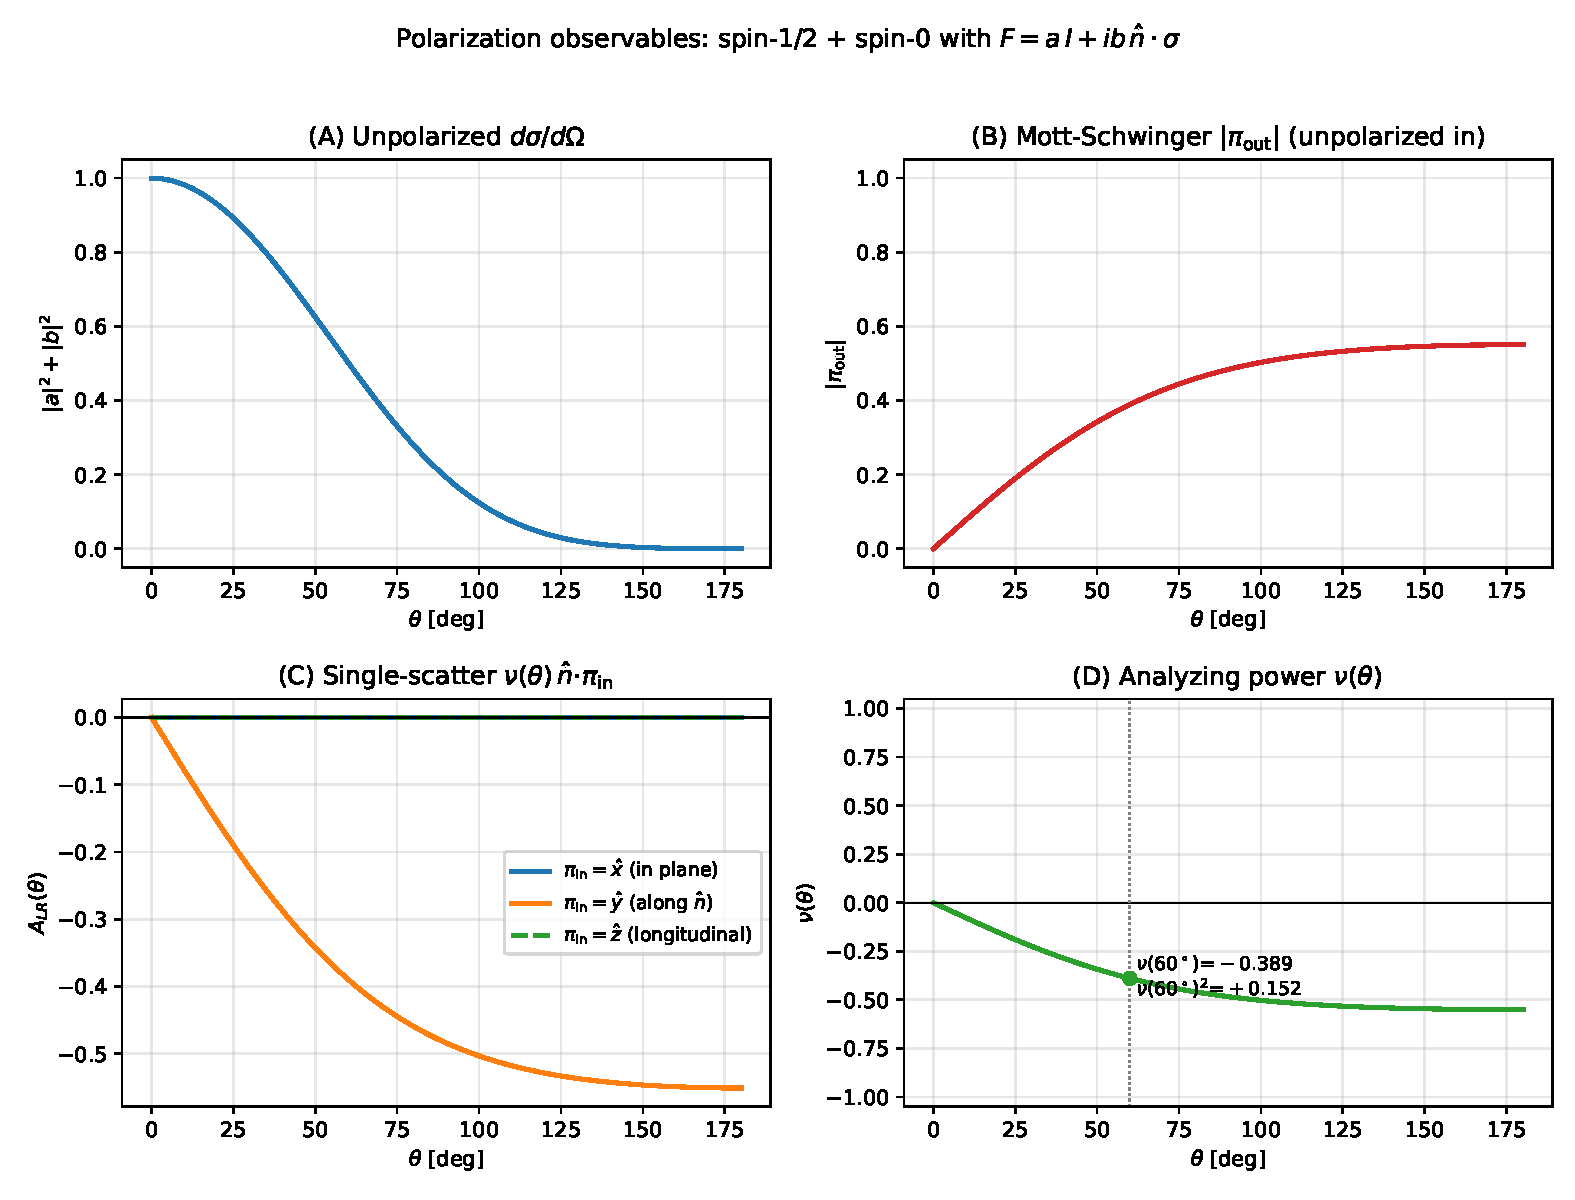
\includegraphics[width=0.95\linewidth]{ch04_polarization}
    \caption{自旋 $1/2$ + 自旋 $0$ 极化观测量 (toy 振幅 $a,b$, $\phi=0$). (A) 非极化截面 $|a|^2+|b|^2$ 在前向 ($\theta\!\to\!0$) 集中, 这是 $a$ 中 $\cos(\theta/2)$ 与 Gauss 包络的合成. (B) 非极化入射的出射极化模 $|\bm\pi^{\rm out}|=|\nu|\le 1$, 极大值出现在中等角度——前向 $b\!\to\!0$ 与后向 Gauss 阻尼都使 $\nu\!\to\!0$. (C) 单次散射 $A_{\rm LR}$: $\bm\pi^{\rm in}=\hat{\bm y}$ (沿 $\hat{\bm n}$) 给出非零信号 $=\nu(\theta)$; $\bm\pi^{\rm in}=\hat{\bm x},\hat{\bm z}$ 严格为零, 数值上验证了式 \eqref{eq:spin2p-ex1-general}. (D) analyzing power $\nu(\theta)$: 在 $60^\circ$ 处 $\nu\!\approx\!-0.389$, 对应对称双散射 ($\hat{\bm n}_2=+\hat{\bm n}_1$) 的 $A_{\rm LR}=\nu^2\!\approx\!+0.152$.}\label{fig:numexp-ch04}
\end{figure}

\subsection*{物理讨论}
\begin{itemize}\itemsep=2pt
  \item \textbf{$\hat{\bm n}$ 方向的特殊地位.} 图 (C) 三条曲线同时绘出, 但只有 $\bm\pi^{\rm in}=\hat{\bm y}$ 那一条非零. 这是 \eqref{eq:spin2p-ex1-general} 中 $A_{\rm LR}\propto\hat{\bm n}\!\cdot\!\bm\pi^{\rm in}$ 的直接体现: 散射平面内的极化 ($\hat{\bm x},\hat{\bm z}$) 不耦合到 single-scatter asymmetry, 平面外法向极化 ($\hat{\bm y}$) 才耦合. 这是 \emph{宇称}与 \emph{旋转不变性}的联合后果——$F$ 中能出现的唯一 $\bm\sigma$ 组合就是 $\hat{\bm n}\!\cdot\!\bm\sigma$ (轴向赝矢量).
  \item \textbf{Cross section vs.\ 极化的互补性.} 图 (A) 与 (D) 各自只看到一半信息: 非极化截面 $|a|^2+|b|^2$ 完全不含 $\arg(ab^*)$, 而 analyzing power $\nu\propto\Im(ab^*)$ 恰好提取相位差. 实验上若只测 $\rmd\sigma/\rmd\Omega$ 不可能拆出 $a,b$; 测了 $\nu$ (双散射或极化靶) 才能反演振幅相位.
  \item \textbf{相位 0.6 的角色.} 把代码中 $b(\theta)$ 的 $\rme^{\rmi\,0.6}$ 改成 $\rme^{\rmi\,0}$ 会让 $\nu\equiv 0$, (B)(C)(D) 整体塌缩到零线 (而 (A) 几乎不变). 这从数值上展示了 \emph{极化观测量是相位敏感探针}.
  \item \textbf{双散射放大.} $\nu(60^\circ)\!\approx\!-0.39$ 在单次散射截面里被 $|a|^2+|b|^2$ 平均掉, 不可观测; 但接成 $\theta_1=\theta_2=60^\circ$ 的双散射后 $A_{\rm LR}=\nu^2\!\approx\!0.15$ ($\sim 15\%$) 直接出现在左/右探测器的计数差异中——这就是 Mott (1929--32), Schwinger (1948) 测量 spin--orbit 振幅相位的实验原理.
  \item \textbf{扩展.} 把 $a,b$ 换成真实物理输入 (如 partial-wave 展开 $a=\sum_\ell[(\ell+1)f_\ell^++\ell f_\ell^-]P_\ell$, $b$ 为相应的 spin-flip 组合) 即可对真实弹性散射做同样的分析. 第\ref{ch:morespin}章会扩展到自旋 $1/2$ + 自旋 $1/2$, 此时 $F$ 含 $5$ 个独立 Wolfenstein 振幅, 极化观测量集合也相应丰富.
\end{itemize}

\chapter{对称性与不变性原理 (Invariance Principles)}\label{ch:invariance}

对称性 (symmetry) 是物理学中最强有力的分析工具之一. 一个系统如果在某一组变换下不变, 我们就说该系统具有相应的对称性, 也称为不变性 (invariance). 经典力学中, Nöther 定理告诉我们: 系统的 Lagrange 量如果具有一个连续对称性, 则相应地有一个守恒律 (conservation law); 例如, 平移对称性对应动量守恒, 转动对称性对应角动量守恒, 时间平移对称性对应能量守恒.

在量子力学中, 对称性变换对应于 Hilbert 空间 $\Hilb$ 上的一个算符 $U$. 由 Wigner 定理, 该算符或者是幺正 (unitary) 算符, 或者是反幺正 (anti-unitary) 算符. 若 $U$ 与 Hamilton 量对易, $[U,H]=0$, 则
\begin{itemize}
  \item 若 $U$ 是连续变换, 其生成元 (generator) 是 Hermite 算符, 对应一个守恒力学量;
  \item 若 $U$ 是分立变换 (如宇称, 时间反演), 则 $U$ 本身就是 Hermite (或反 Hermite) 的守恒算符.
\end{itemize}

在散射理论中, 对称性将对 $S$ 散射矩阵元施加很强的限制. 利用对称性分析, 往往不需要具体计算散射矩阵元, 即可得到一些有用的结论 (例如选择定则, 角分布的特征, 矩阵元之间的约束关系等).

本章我们系统地讨论散射理论中的对称性原理: 平移不变性, 转动不变性, 宇称变换 $\mathsf{P}$, 时间反演 $\mathsf{T}$, 以及自旋粒子情形下的角动量表象. 主要参考 Taylor 教科书相应章节.


\section{对称性变换与 \texorpdfstring{$S$}{S} 矩阵的一般框架}

设系统的对称群为 $\mathcal{G}$, $\mathcal{G}$ 在 $\Hilb$ 上有幺正 (或反幺正) 表示 $g\mapsto U(g)$. 对自由 Hamilton 量 $H_0$ 和总 Hamilton 量 $H=H_0+V$, 我们说系统具有对称性 $\mathcal{G}$, 即
\begin{equation}
[U(g),H_0]=0, \qquad [U(g),H]=0, \qquad \forall g\in\mathcal{G}.
\end{equation}

\begin{theorem}[对称性与 $S$ 算符]\label{thm:symS}
若 $[U(g),H_0]=[U(g),H]=0$, 则 Møller 算符 $\Omega_\pm$ 与 $U(g)$ 对易, $S$ 算符也与 $U(g)$ 对易:
\begin{equation}
[U(g),\Omega_\pm]=0, \qquad [U(g),\Smat]=0.
\end{equation}
\end{theorem}

\begin{proof*}
由
\[
\Omega_\pm =\lim_{t\to \mp\infty} \rme^{\rmi Ht}\rme^{-\rmi H_0 t},
\]
对于幺正 $U=U(g)$ 有
\[
U\Omega_\pm = \lim_{t\to \mp\infty} U \rme^{\rmi Ht}\rme^{-\rmi H_0 t}
=\lim_{t\to \mp\infty} \rme^{\rmi Ht}\rme^{-\rmi H_0 t} U =\Omega_\pm U,
\]
所以 $[U,\Omega_\pm]=0$. 由 $\Smat=\Omega_-^\dagger \Omega_+$ 立得 $[U,\Smat]=0$, 即
\begin{equation}
U^\dagger(g)\,\Smat\,U(g)=\Smat.
\end{equation}
对于反幺正变换 (时间反演) 推导稍有不同, 我们将在 \S\ref{sec:T} 单独处理.
\end{proof*}

由 $[U(g),\Smat]=0$, 散射矩阵元满足
\begin{equation}\label{eq:S-invariance}
\matel{\chi}{\Smat}{\phi}=\matel{U(g)\chi}{\Smat}{U(g)\phi}=\matel{\chi_g}{\Smat}{\phi_g},
\end{equation}
即 in 态和 out 态同时作变换后, 矩阵元不变, $\phi\to\chi$ 过程的散射几率, 因而散射截面也不变. 这是所有对称性结论的出发点.

\begin{remark}
后面在二粒子散射中, 我们将利用 $\Smat=\mathbf{1}_{cm}\otimes \Smat_{rel}$ 把质心运动分离掉, 只研究相对运动部分. 因此本章中所谓 ``单粒子'' 散射其实指相对运动 (在 $\Hilb_{rel}$ 上).
\end{remark}


\section{平移对称性与动量守恒}\label{sec:translation}

\subsection{平移算符}

定义平移算符 (translation operator)
\begin{equation}
D(\mathbf{a})=\rme^{-\rmi \mathbf{P}\cdot\mathbf{a}},
\end{equation}
其中 $\mathbf{P}$ 是总动量算符. $D(\mathbf{a})$ 是幺正的 (因 $\mathbf{P}$ 是 Hermite 算符).

\begin{itemize}
  \item 系统的平移不变性要求 $D^\dagger(\mathbf{a})HD(\mathbf{a})=H$, 即 $[H,D(\mathbf{a})]=0$, 等价地 $[\mathbf{P},H]=0$, 即总动量守恒.
  \item 对二粒子系统, $H=H_0+V$, 自由 $H_0$ 自动平移不变, $[H_0,D(\mathbf{a})]=0$. 当 $V=V(\mathbf{x}_1-\mathbf{x}_2)$ 仅依赖相对坐标时 $V$ 也平移不变, 所以 $H$ 平移不变.
\end{itemize}

由 Theorem \ref{thm:symS},
\begin{equation}
[D(\mathbf{a}),\Omega_\pm]=0,\qquad [D(\mathbf{a}),\Smat]=0,
\end{equation}
即 $D^\dagger(\mathbf{a})\Smat D(\mathbf{a})=\Smat$.

\subsection{动量守恒}

由 \eqref{eq:S-invariance},
\begin{equation}
\matel{\chi}{\Smat}{\phi}=\matel{\chi_{\mathbf{a}}}{\Smat}{\phi_{\mathbf{a}}},
\end{equation}
平移之后矩阵元不变. 因 $\mathbf{a}$ 任意, 故 $[\mathbf{P},\Smat]=0$. 取动量本征态 $\ket{\mathbf{p}}$ ($\mathbf{P}\ket{\mathbf{p}}=\mathbf{p}\ket{\mathbf{p}}$), 在 $S-1$ 矩阵元上插入对易子,
\begin{align}
0&=\matel{\mathbf{p}'}{[\mathbf{P},\Smat]}{\mathbf{p}}=(\mathbf{p}'-\mathbf{p})\matel{\mathbf{p}'}{\Smat}{\mathbf{p}},
\end{align}
所以
\begin{equation}\label{eq:Sdelta}
\matel{\mathbf{p}'}{\Smat}{\mathbf{p}}\propto \delta_3(\mathbf{p}'-\mathbf{p}),\qquad \matel{\mathbf{p}'}{\Smat-\mathbf{1}}{\mathbf{p}}\propto \delta_3(\mathbf{p}'-\mathbf{p})|_{\text{forward}}+\cdots.
\end{equation}
更准确地, 在质心系中, 二粒子系统的总动量守恒已被分离, $\Smat_{rel}$ 作用在相对动量空间上, 矩阵元含一个 $\delta_3(\mathbf{p}'-\mathbf{p})$ (与 $\delta(E'-E)$ 一起出现的方式见前面散射截面一章).


\section{转动对称性与角动量守恒}\label{sec:rotation}

\subsection{转动算符}

定义转动算符
\begin{equation}
\mathsf{R}(\bm{\alpha})=\rme^{-\rmi \bm{\alpha}\cdot \bar{\mathbf{J}}},
\end{equation}
其中 $\bar{\mathbf{J}}$ 为总角动量算符, $\bm{\alpha}=\alpha\,\mathbf{u}$, $\mathbf{u}$ 为转轴方向单位矢量, $\alpha$ 为顺时针 (按右手定则) 转角.

二粒子系统的转动不变性: $\mathsf{R}^\dagger(\bm{\alpha})H\mathsf{R}(\bm{\alpha})=H$ 及 $\mathsf{R}^\dagger H_0 \mathsf{R}=H_0$. 由 Theorem \ref{thm:symS},
\begin{equation}
[\mathsf{R}(\bm{\alpha}),\Omega_\pm]=0,\qquad [\mathsf{R}(\bm{\alpha}),\Smat]=0.
\end{equation}
$\bm{\alpha}$ 任意 $\Rightarrow [\bar{\mathbf{J}},\Smat]=0$, 总角动量守恒.

\subsection{分离质心: 内部角动量}

由 $\Smat=\mathbf{1}_{cm}\otimes \Smat_{rel}$, 总角动量
\begin{equation}
\bar{\mathbf{J}}=\mathbf{J}_1+\mathbf{J}_2 =\bar{\mathbf{X}}\times \bar{\mathbf{P}} + \mathbf{X}\times\mathbf{P} +\mathbf{S}_1+\mathbf{S}_2 = \bar{\mathbf{X}}\times \bar{\mathbf{P}} + \mathbf{J},
\end{equation}
其中 $\bar{\mathbf{X}}\times\bar{\mathbf{P}}$ 为质心轨道角动量, 作用在 $\Hilb_{cm}$ 上; $\mathbf{J}=\mathbf{X}\times \mathbf{P}+\mathbf{S}_1+\mathbf{S}_2$ 为 ``内部'' 角动量, 作用在 $\Hilb_{rel}$ 上. 由
\[
[\bar{\mathbf{J}},\Smat]=0\;\Longleftrightarrow\;[\mathbf{J},\Smat_{rel}]=0,
\]
研究 $\Smat$ 受转动的限制等价于研究 $\mathbf{J}$ 与 $\Smat_{rel}$ 的对易性. 下文若无特殊说明, $\mathbf{J}, \Smat$ 均指相对运动部分.

\subsection{无自旋情形: 散射振幅依赖 \texorpdfstring{$\theta$}{theta}}

对于无自旋两粒子散射的相对运动部分:
\begin{itemize}
  \item $H_0$ 自动转动不变, 所以只要 $V$ 转动不变 (即 $V(\mathbf{x})=V(r)$, $r=|\mathbf{x}|$), $H$ 即转动不变, $\Smat$ 与转动 $\mathsf{R}$ 对易.
  \item 由转动不变性, $\matel{\mathbf{p}'}{\Smat}{\mathbf{p}}=\matel{\mathbf{p}'_{R}}{\Smat}{\mathbf{p}_{R}}$, 因此散射振幅 $f(\mathbf{p}'\leftarrow \mathbf{p})=f(\mathbf{p}'_{R}\leftarrow \mathbf{p}_{R})$.
\end{itemize}

无对称性的散射振幅 $f(\mathbf{p}'\leftarrow \mathbf{p})$ 本来有 5 个独立变量 ($\mathbf{p}, \mathbf{p}'$ 方向 4 个 +能量 1 个; 由能量守恒 $|\mathbf{p}'|=|\mathbf{p}|=p$). 转动对称性消掉 3 个转动自由度: 总可以 (i) 把 $\mathbf{p}$ 转到 $z$ 轴, (ii) 把 $\mathbf{p}'$ 转到包含 $z$ 轴的某一特定平面 (如 $xz$ 平面). 因此独立变量只剩 2 个, 可取
\begin{equation}
E_p=\frac{p^2}{2\mathrm{m}},\qquad \theta=\angle(\mathbf{p},\mathbf{p}'),
\end{equation}
即 $f=f(E,\theta)$. 这就是无自旋粒子的转动不变散射振幅与轴对称性的来源.

\subsection{角动量基与分波 (Partial wave) 展开}

对无自旋情形, 内部角动量 $\mathbf{J}=\mathbf{L}=\mathbf{X}\times\mathbf{P}$ 即轨道角动量. 单粒子 $H_0,\mathbf{L}^2,L_3$ 构成对易力学量完全集 (CSCO), 描述束缚态的渐近行为. 取共同本征基 $\ket{E,l,m}$,
\begin{equation}
H_0\ket{E,l,m}=E\ket{E,l,m},\quad \mathbf{L}^2\ket{E,l,m}=l(l+1)\ket{E,l,m},\quad L_3\ket{E,l,m}=m\ket{E,l,m}.
\end{equation}
自由 Hamilton 解: 径向方程 $\bigl(\partial_\rho^2 -\frac{l(l+1)}{\rho^2}+1\bigr)R_l(\rho)=0$, $\rho=pr$, $p=\sqrt{2\mathrm{m}E}$, 解为 Riccati-Bessel 函数 $\hat{j}_l(z)=z j_l(z)$. 坐标表象波函数为
\begin{equation}
\inn{\mathbf{x}}{E,l,m}=\rmi^l\Bigl(\frac{2\mathrm{m}}{\pi p}\Bigr)^{1/2}\frac{1}{r}\hat{j}_l(pr)\,Y_l^m(\hat{\mathbf{x}}),
\end{equation}
归一化为
\[
\inn{E',l',m'}{E,l,m}=\delta(E'-E)\delta_{l'l}\delta_{m'm},\qquad p\equiv (2\mathrm{m}E)^{1/2}.
\]
$\ket{E,l,m}$ 是 improper (delta 归一化的非平方可积) 矢量.

\begin{theorem}[转动不变下 $\Smat$ 在角动量基中对角]\label{thm:S-diag}
若 $[\mathbf{L},\Smat]=0$, 则
\begin{equation}\label{eq:Sdiag-l}
\matel{E'l'm'}{\Smat}{Elm}=\delta(E'-E)\delta_{l'l}\delta_{m'm}\,\mathsf{s}_l(E),
\end{equation}
其中 $\mathsf{s}_l(E)$ 与 $m$ 无关. (这是 Wigner-Eckart 定理的特例.)
\end{theorem}

\begin{proof*}
由 $[\mathbf{L},\Smat]=0$, $L_\pm \Smat=\Smat L_\pm$, 故
\[
\matel{\ldots,m+1}{\Smat}{\ldots,m+1}=\matel{\ldots,m}{\Smat}{\ldots,m},
\]
所以矩阵元与 $m$ 无关. 角动量算符 ($\mathbf{L}^2,L_3$) 与 $H_0$ 对易, $\Smat$ 在能量与 $(l,m)$ 上同时对角: 故得 \eqref{eq:Sdiag-l}.
\end{proof*}

由 $\Smat$ 幺正性 ($\Smat^\dagger \Smat=1$), $|\mathsf{s}_l(E)|=1$, 故 $\mathsf{s}_l$ 是纯位相,
\begin{equation}\label{eq:phaseshift}
\mathsf{s}_l(E)=\rme^{2\rmi \delta_l(E)}.
\end{equation}
$\delta_l(E)$ 称为相移 (phase shift), 由 $\rme^{2\rmi(\delta_l+n\pi)}=\rme^{2\rmi\delta_l}$, $\delta_l$ 模 $\pi$ 取值, $n\in \mathbb{Z}$.

\subsection{动量基与角动量基的转换 -- 分波展开公式}

利用平面波分解
\begin{equation}
\rme^{\rmi\mathbf{k}\cdot\mathbf{x}}=\frac{4\pi}{kr}\sum_{l,m}\rmi^l\hat{j}_l(kr)Y_l^m(\hat{\mathbf{x}})Y_l^{m*}(\hat{\mathbf{k}}),
\end{equation}
有
\begin{equation}
\inn{\mathbf{p}}{E,l,m}=(\mathrm{m}p)^{-1/2}\delta(E_p-E)\,Y_l^m(\hat{\mathbf{p}}).
\end{equation}
由此
\begin{align}
\matel{\mathbf{p}'}{(\Smat-\mathbf{1})}{\mathbf{p}}
&=\frac{\rmi}{2\pi \mathrm{m}}\delta(E_{p'}-E_p)\,f(\mathbf{p}'\leftarrow \mathbf{p}) \nonumber\\
&=\sum_{l,m}\int dE\,\matel{\mathbf{p}'}{(\Smat-\mathbf{1})}{E,l,m}\inn{E,l,m}{\mathbf{p}}\nonumber\\
&=\sum_{l,m}(\mathsf{s}_l(E)-1)\inn{\mathbf{p}'}{E,l,m}\inn{E,l,m}{\mathbf{p}}\nonumber\\
&=\frac{1}{\mathrm{m}p}\delta(E_{p'}-E_p)\sum_{l,m}Y_l^m(\hat{\mathbf{p}}')[\mathsf{s}_l(E)-1]Y_l^{m*}(\hat{\mathbf{p}}).
\end{align}
对比得
\begin{equation}
f(\mathbf{p}'\leftarrow \mathbf{p})=\frac{2\pi}{\rmi p}\sum_{l,m}Y_l^m(\hat{\mathbf{p}}')[\mathsf{s}_l(E)-1]Y_l^{m*}(\hat{\mathbf{p}}).
\end{equation}
取 $\hat{\mathbf{p}}=\hat{z}$, $Y_l^m(\hat{z})=\sqrt{(2l+1)/(4\pi)}\,\delta_{m,0}$ (仅 $m=0$ 不为零), 利用 $P_l(\cos\theta)=\sqrt{4\pi/(2l+1)}\,Y_l^0(\theta,\varphi)$:

\begin{theorem}[分波展开]\label{thm:partial-wave}
具有转动不变性的无自旋单粒子势散射, 散射振幅展为分波 (partial wave) 形式
\begin{equation}\label{eq:partial-wave}
f(E,\theta)=\sum_{l=0}^{\infty}(2l+1)f_l(E)P_l(\cos\theta),
\end{equation}
其中
\begin{equation}\label{eq:fl}
f_l(E)=\frac{\mathsf{s}_l(E)-1}{2\rmi p}=\frac{\rme^{2\rmi\delta_l(E)}-1}{2\rmi p}=\frac{\rme^{\rmi\delta_l}\sin\delta_l(E)}{p}
\end{equation}
称为分波振幅 (partial wave amplitude). 反过来
\[
f_l(E)=\frac{1}{2}\int_{-1}^{1}\rmd(\cos\theta)\,f(E,\theta)P_l(\cos\theta).
\]
\end{theorem}

\subsection{分波散射截面与幺正性界 (unitary bound)}

微分散射截面 $\rmd\sigma/\rmd\Omega=|f|^2$ 用分波振幅写成
\begin{equation}
\frac{\rmd\sigma}{\rmd\Omega}=\sum_{l,l'=0}^{\infty}(2l+1)(2l'+1)f_l^*(E)f_{l'}(E)P_l(\cos\theta)P_{l'}(\cos\theta).
\end{equation}
对 $\theta,\varphi$ 积分, 利用 $\int P_l P_{l'}\sin\theta\,\rmd\theta=\frac{2}{2l+1}\delta_{ll'}$,
\begin{equation}
\sigma(p)=\sum_l\sigma_l(p),\qquad \sigma_l(p)=4\pi(2l+1)|f_l(p)|^2=\frac{4\pi(2l+1)\sin^2\delta_l}{p^2}.
\end{equation}

由 $|\sin\delta_l|\le 1$,
\begin{equation}\label{eq:unitarity-bound}
\sigma_l(p)\le \frac{4\pi(2l+1)}{p^2},
\end{equation}
此式称为幺正性界 (unitary bound), 仅在 $\delta_l=k\pi/2$ ($k$ 奇数) 时取等号.

\begin{remark}
低能时仅有少数几个分波相移非零, 无穷分波求和变成有限项求和. 这是低能散射 (例如 $s$ 波 ($l=0$) 主导) 处理的物理基础.
\end{remark}

\begin{example}[$s$ 波散射]
低能极限下, 若 $\rmd\sigma/\rmd\Omega$ 与方向 $\theta$ 无关, 则只有 $l=0$ 贡献. 此时
\begin{equation}
f(E,\theta)=\frac{1}{2\rmi p}(\rme^{2\rmi\delta_0(E)}-1)=\frac{\rme^{\rmi \delta_0}\sin\delta_0(E)}{p}.
\end{equation}
$\rmd\sigma/\rmd\Omega=|f|^2=\sin^2\delta_0/p^2$ 给出 $|\sin\delta_0|$ 的大小.
\end{example}


\section{宇称变换 \texorpdfstring{$\mathsf{P}$}{P}}\label{sec:parity}

\subsection{宇称的定义与基本性质}

宇称变换 $\mathsf{P}$ (又称空间反演, parity, space inversion) 为分立对称变换:
\begin{equation}
\mathbf{x}\to -\mathbf{x},\qquad \mathbf{p}\to -\mathbf{p}.
\end{equation}
作用在波函数上:
\begin{equation}
\mathsf{P}\psi(\mathbf{x})=\psi(-\mathbf{x}),\qquad (\mathsf{P}\psi)(\mathbf{p})=\psi(-\mathbf{p}),
\end{equation}
即在动量基矢上 $\mathsf{P}\ket{\mathbf{x}}=\ket{-\mathbf{x}}$, $\mathsf{P}\ket{\mathbf{p}}=\ket{-\mathbf{p}}$. 显然 $\mathsf{P}$ 幺正且 $\mathsf{P}^2=\mathbf{1}$, 故 $\mathsf{P}=\mathsf{P}^\dagger$, 本征值 $\mathsf{p}=\pm 1$.

\subsection{宇称不变与守恒}

非相对论情形, $H=H_0+V(\mathbf{x})$. $\mathsf{P}$ 变换下 $H_0$ 不变 (因 $H_0$ 仅依赖 $\mathbf{p}^2$). 若势满足 $V(\mathbf{x})=V(-\mathbf{x})$, 则 $[\mathsf{P},V]=[\mathsf{P},H]=0$, 由 Theorem \ref{thm:symS}
\[
\mathsf{P}^\dagger \Smat \mathsf{P}=\Smat,\qquad [\mathsf{P},\Smat]=0.
\]

设 $\ket{\phi}$ 有确定宇称 $\mathsf{P}\ket{\phi}=\mathsf{p}\ket{\phi}$ ($\mathsf{p}=\pm 1$), 类似 $\mathsf{P}\ket{\phi'}=\mathsf{p}'\ket{\phi'}$, 则
\[
0=\matel{\phi}{[\mathsf{P},\Smat]}{\phi'}=(\mathsf{p}-\mathsf{p}')\matel{\phi}{\Smat}{\phi'},
\]
故 $\matel{\phi}{\Smat}{\phi'}$ 仅在 $\mathsf{p}=\mathsf{p}'$ 时不为零, 即宇称守恒 (parity conservation).

\subsection{在动量基上}

由 $\mathsf{P}\ket{\mathbf{p}}=\ket{-\mathbf{p}}$ (取相位为 1),
\begin{equation}
\matel{\mathbf{p}'}{\Smat}{\mathbf{p}}=\matel{-\mathbf{p}'}{\Smat}{-\mathbf{p}},\qquad f(\mathbf{p}'\leftarrow \mathbf{p})=f(-\mathbf{p}'\leftarrow -\mathbf{p}).
\end{equation}

\begin{remark}
若已经具有转动对称性, 上式自动成立 (因为绕散射平面法线轴转 $\pi$ 等价于反演). 但一般而言, 转动对称性与 $\mathsf{P}$ 对称性是独立的.
\end{remark}


\section{时间反演 \texorpdfstring{$\mathsf{T}$}{T}}\label{sec:T}

\subsection{Wigner 定理与反幺正变换}

\begin{theorem}[Wigner]
若一对称性变换 $\ket{\psi}\to \ket{\psi'}$ 保持所有跃迁概率不变, 则通过调整位相, 可以存在一个幺正变换 $U$ 或一个反幺正变换 (anti-unitary) $W$ 使得
\[
\ket{\psi'}=U\ket{\psi}\quad \text{或}\quad \ket{\psi'}=W\ket{\psi},\quad \forall \ket{\psi}.
\]
\end{theorem}

反幺正变换 $W:\Hilb\to \Hilb$ 是一一映射, 保模长 $\inn{W\chi}{W\chi}=\inn{\chi}{\chi}$, 但是是反线性 (anti-linear) 算符:
\begin{equation}
W(a\ket{\psi}+b\ket{\phi})=a^*W\ket{\psi}+b^*W\ket{\phi}.
\end{equation}

平移, 转动, 宇称都是幺正算符. 时间反演 $\mathsf{T}$ 则是反幺正的, 原因如下:
\begin{itemize}
  \item 两个反幺正算符乘积是幺正的.
  \item 一个幺正算符乘以一个反幺正算符是反幺正的.
  \item 对线性算符 $A$, 有左作用规则 $\matel{\phi}{A}{\psi}=(\bra{\phi}A)\ket{\psi}=\inn{A^\dagger \phi}{\psi}$.
  \item 对反线性算符 $W$ 的左右作用规则: $\inn{\phi}{W\psi}=\inn{W^\dagger \phi}{\psi}^*$ (复共轭).
  \item 反幺正性: $\inn{W\chi}{W\phi}=\inn{\chi}{\phi}^*$, $W^\dagger W=WW^\dagger=\mathbf{1}$.
\end{itemize}

\subsection{时间反演与 Hamilton 量: \texorpdfstring{$\mathsf{T} \rmi=-\rmi \mathsf{T}$}{T i = -i T}}

若 $\psi(t)$ 满足含时 Schrödinger 方程
\[
\rmi \partial_t \psi(t)=H\psi(t),\Rightarrow -\rmi \partial_t \psi(-t)=H\psi(-t).
\]
我们希望 $\psi(-t)$ 经过适当变换 $\psi_{\mathsf{T}}(t)\equiv \mathsf{T}\psi(-t)$ 后 ($\mathsf{T}$ 待定, 幺正或反幺正) 仍满足含时 Schrödinger 方程
\[
\rmi \partial_t \psi_{\mathsf{T}}(t)=H\psi_{\mathsf{T}}(t).
\]
代入:
\begin{align*}
\rmi\partial_t \mathsf{T}\psi(-t)&=H\mathsf{T}\psi(-t)\;\Rightarrow\; \mathsf{T}\,\rmi\partial_t \psi(-t)=H\mathsf{T}\psi(-t)\\
&\Rightarrow \mathsf{T}\,\rmi(-\rmi)H\psi(-t)/\!\rmi=H\mathsf{T}\psi(-t)\\
&\Rightarrow \mathsf{T}\,\rmi H=-\rmi H\mathsf{T}\quad(\text{即 } \mathsf{T}(\rmi)=-\rmi\mathsf{T}).
\end{align*}

\begin{itemize}
  \item 若 $\mathsf{T}$ 幺正 ($\mathsf{T}\rmi=\rmi \mathsf{T}$), 则 $\mathsf{T} H=-H\mathsf{T}$, 对能量本征态 $\ket{E}$ ($H\ket{E}=E\ket{E}$), 应有 $H\mathsf{T}\ket{E}=-E\mathsf{T}\ket{E}$, 即对应一个能量为 $-E$ 的态. 物理上能谱无界 $E\in[0,\infty)$ 时这会出现负能态, 不合理.
  \item 若 $\mathsf{T}$ 反幺正 ($\mathsf{T}\rmi=-\rmi\mathsf{T}$), $\mathsf{T} H= H\mathsf{T}$, 不会有负能量态出现.
\end{itemize}
故时间反演必然是反幺正算符.

\subsection{基本变换规则}

时间反演下,
\[
\mathbf{x}\to \mathbf{x},\quad \mathbf{p}\to -\mathbf{p},\quad \mathbf{J}\to -\mathbf{J}.
\]
经典上 $\mathbf{x},\mathbf{p},\mathbf{J}$ 都是数; 量子上是算符. 通过适当选择基矢相位, 可以取
\begin{equation}\label{eq:Tbasis}
\mathsf{T}\ket{\mathbf{x}}=\ket{\mathbf{x}},\qquad \mathsf{T}\ket{\mathbf{p}}=\ket{-\mathbf{p}}.
\end{equation}
对任意态 $\ket{\psi}=\int \rmd^3x\,\psi(\mathbf{x})\ket{\mathbf{x}}$, 由 $\mathsf{T}$ 反线性:
\begin{align}
\mathsf{T}\ket{\psi}&=\int \rmd^3x\,\psi^*(\mathbf{x})\mathsf{T}\ket{\mathbf{x}}=\int \rmd^3x\,\psi^*(\mathbf{x})\ket{\mathbf{x}}\nonumber\\
\Rightarrow \psi_{\mathsf{T}}(\mathbf{x})&=\psi^*(\mathbf{x}),\qquad \psi_{\mathsf{T}}(\mathbf{p})=\psi^*(-\mathbf{p}).
\end{align}

\subsection{无自旋势散射的 \texorpdfstring{$\mathsf{T}$}{T} 不变性}

无自旋粒子定域势 (无磁场) 的情形: $V=V(\mathbf{x})$, $\mathsf{T}^\dagger V \mathsf{T}=V^*(\mathbf{x})$ (因 $\mathsf{T}$ 反幺正且 $\mathbf{x}$ 不变). 故
\[
[\mathsf{T},H]=0\quad\Longleftrightarrow\quad V^*(\mathbf{x})=V(\mathbf{x}),
\]
即势取实值. 演化算符 $\mathsf{T}\rme^{\rmi Ht}\mathsf{T}^\dagger=\rme^{-\rmi Ht}$ (因 $\mathsf{T}\rmi=-\rmi\mathsf{T}$).

Møller 算符:
\[
\mathsf{T}\Omega_\pm \mathsf{T}^\dagger=\mathsf{T}\lim_{t\to \mp\infty}\rme^{\rmi Ht}\rme^{-\rmi H_0 t}\mathsf{T}^\dagger
=\lim_{t\to \mp\infty}\rme^{-\rmi Ht}\rme^{\rmi H_0 t}=\Omega_\mp,
\]
即 $\mathsf{T}\Omega_\pm=\Omega_\mp\mathsf{T}$, 或 $\Omega_\pm =\mathsf{T}^\dagger\Omega_\mp \mathsf{T}$.

对 $\Smat=\Omega_-^\dagger \Omega_+$:
\[
\mathsf{T}\Smat \mathsf{T}^\dagger=\mathsf{T}\Omega_-^\dagger \mathsf{T}^\dagger\,\mathsf{T}\Omega_+\mathsf{T}^\dagger=\Omega_+^\dagger \Omega_-=\Smat^\dagger,
\]
所以
\begin{equation}\label{eq:T-S}
\Smat=\mathsf{T}^\dagger \Smat^\dagger \mathsf{T}.
\end{equation}

$\mathsf{T}$ 不变下 $S$ 矩阵元的关系: 设 $\inn{\chi_{\mathsf{T}}}{\phi_{\mathsf{T}}}$ 等记号表示 $\chi_{\mathsf{T}}=\mathsf{T}\chi$ 等. 由反幺正性
\begin{align}
\inn{\chi}{\Smat\phi}&=\inn{\chi}{\mathsf{T}^\dagger \Smat^\dagger \mathsf{T}\phi}=\inn{\mathsf{T}\chi}{\Smat^\dagger \mathsf{T}\phi}^*=\inn{\chi_{\mathsf{T}}}{\Smat^\dagger \phi_{\mathsf{T}}}^*\nonumber\\
&=\inn{\phi_{\mathsf{T}}}{\Smat \chi_{\mathsf{T}}},
\end{align}
即 $w(\phi\leftarrow \chi)=w(\chi_{\mathsf{T}}\leftarrow \phi_{\mathsf{T}})$ (跃迁概率反向但 in/out 互换).

在动量表象 $\matel{\mathbf{p}'}{\Smat}{\mathbf{p}}=\matel{-\mathbf{p}}{\Smat}{-\mathbf{p}'}$, 即
\begin{equation}\label{eq:T-amp}
f(\mathbf{p}'\leftarrow \mathbf{p})=f(-\mathbf{p}\leftarrow -\mathbf{p}').
\end{equation}
此即 ``反应平衡 (reciprocity)'' 关系.


\section{有自旋粒子的转动}\label{sec:spin-rotation}

对于无自旋粒子, 基矢 $\ket{\mathbf{p}}$ 完全描述; 有自旋粒子需要额外的自旋指标 $\ket{\mathbf{p},\xi}$.

\subsection{自旋部分的转动表示}

考虑自旋态 $\ket{\chi}\in \Hilb_s$ (自旋空间), 转动下变换
\begin{equation}
\ket{\chi}\stackrel{\mathsf{R}}{\longrightarrow}\ket{\chi_R}=\mathsf{R}_s\ket{\chi},\qquad \mathsf{R}_s=\rme^{-\rmi \bm{\alpha}\cdot \mathbf{S}},
\end{equation}
$\mathbf{S}$ 为对应总自旋算符. 选自旋基 $\ket{\xi}$,
\[
\mathsf{R}_s\ket{\xi}=\sum_{\xi'}\ket{\xi'}\matel{\xi'}{\mathsf{R}_s}{\xi}.
\]
特殊地, 选 $S_3$ 本征态 $\ket{sm}$,
\[
\mathsf{R}_s(\alpha\hat{3})\ket{sm}=\rme^{-\rmi \alpha S_3}\ket{sm}=\rme^{-\rmi \alpha m}\ket{sm}.
\]

整个 Hilbert 空间为 $\Hilb=\Hilb_p\otimes \Hilb_s$, 一般态 $\ket{\mathbf{p},\xi}=\ket{\mathbf{p}}\otimes \ket{\xi}$. 完整转动 $\mathsf{R}=\mathsf{R}_p\otimes \mathsf{R}_s$ 作用:
\begin{equation}
\mathsf{R}\ket{\mathbf{p},\xi}=\ket{\mathbf{p}_R}\otimes \sum_{\xi'}\ket{\xi'}\matel{\xi'}{\mathsf{R}_s}{\xi}=\sum_{\xi'}\ket{\mathbf{p}_R,\xi'}\mathsf{R}_{\xi'\xi}.
\end{equation}

\subsection{有自旋下的转动不变性}

$\Smat$ 转动不变: $\Smat=\mathsf{R}^\dagger \Smat \mathsf{R}$, 矩阵元
\[
\matel{\mathbf{p}',\xi'}{\Smat}{\mathbf{p},\xi}=\matel{\mathbf{p}',\xi'}{\mathsf{R}^\dagger \Smat \mathsf{R}}{\mathbf{p},\xi}=\sum_{\bar\xi,\bar\xi'}\mathsf{R}^*_{\bar\xi'\xi'}\matel{\mathbf{p}'_R,\bar\xi'}{\Smat}{\mathbf{p}_R,\bar\xi}\mathsf{R}_{\bar\xi\xi}.
\]
对应的散射振幅 $F(\mathbf{p}'\leftarrow \mathbf{p})=\{f_{\xi'\xi}(\mathbf{p}'\leftarrow \mathbf{p})\}$ 由
\begin{equation}
\matel{\mathbf{p}',\xi'}{\Smat-\mathbf{1}}{\mathbf{p},\xi}=\frac{\rmi}{2\pi \mathrm{m}}\delta(E_{p'}-E_p)f_{\xi'\xi}(\mathbf{p}'\leftarrow \mathbf{p})
\end{equation}
是一个 $(2s_1+1)(2s_2+1)\times (2s_1+1)(2s_2+1)$ 的矩阵.

\subsubsection*{利用转动减少独立变量}

选 $\mathbf{p}$ 沿 $\hat{3}$ 方向, $\mathbf{p}'$ 方向 $(\theta,\varphi)$, 基矢取 $S_3$ 本征 $\xi=(m_1,m_2)$ 或 $\xi=(s,m)$. 围绕 $z$ 轴转动 $-\varphi$, $\mathbf{p}, \mathbf{p}'$ 进入 $xz$ 平面:
\begin{align}
\mathsf{R}(-\varphi\hat{3})\ket{\mathbf{p},s,m}&=\rme^{\rmi m\varphi}\ket{\mathbf{p},s,m},\nonumber\\
\mathsf{R}(-\varphi\hat{3})\ket{\mathbf{p}',s,m'}&=\rme^{\rmi m'\varphi}\ket{\mathbf{p}'',s,m'},
\end{align}
故
\begin{align}
\matel{\mathbf{p}',sm'}{\Smat}{\mathbf{p}sm}&=\matel{\mathbf{p}'sm'}{\mathsf{R}^\dagger(-\varphi\hat{3})\Smat \mathsf{R}(-\varphi\hat{3})}{\mathbf{p}sm}\nonumber\\
&=\rme^{\rmi(m-m')\varphi}\matel{\mathbf{p}''sm'}{\Smat}{\mathbf{p}sm},
\end{align}
即
\begin{equation}\label{eq:phivar}
f_{sm',sm}(E,\theta,\varphi)=\rme^{\rmi(m-m')\varphi}f_{sm',sm}(E,\theta,0).
\end{equation}

\begin{example}[自旋 $1/2$ 与自旋 $0$ 散射]
$S_z\ket{\pm}=\pm 1/2\ket{\pm}$, 散射振幅
\[
F(E,\theta,\varphi)=\begin{pmatrix}f_{++}(\mathbf{p}'\leftarrow \mathbf{p})&f_{+-}(\mathbf{p}'\leftarrow \mathbf{p})\\ f_{-+}(\mathbf{p}'\leftarrow \mathbf{p})&f_{--}(\mathbf{p}'\leftarrow \mathbf{p})\end{pmatrix}=\begin{pmatrix}a(E,\theta)& b(E,\theta)\rme^{-\rmi \varphi}\\ c(E,\theta)\rme^{\rmi\varphi}& d(E,\theta)\end{pmatrix}.
\]
其中 $f_{++},f_{--}$ 称为非自旋反转振幅 (spin-nonflip amplitude); $f_{+-},f_{-+}$ 称为自旋反转振幅 (spin-flip amplitude). 4 个独立函数 $a,b,c,d$ 完全确定 $E,\theta$ 给定时的 $F$.
\end{example}


\section{有自旋下的 \texorpdfstring{$\mathsf{P}$}{P} 与 \texorpdfstring{$\mathsf{T}$}{T} 对称性}\label{sec:spin-PT}

\subsection{有自旋下的 \texorpdfstring{$\mathsf{P}$}{P} 对称性}

由 $\mathsf{P}^\dagger \mathbf{J}\mathsf{P}=\mathbf{J}$, $\mathsf{P}^\dagger \mathbf{P}_{op}\mathsf{P}=-\mathbf{P}_{op}$, 故
\[
\mathsf{P}\ket{\mathbf{p},\xi}=\ket{-\mathbf{p},\xi}.
\]
($\mathsf{P}$ 不改变自旋. 实际上还可以有一个相位因子, 此处非相对论弹性散射可设为 $1$.)

对自旋 $1/2$, $\mathsf{P}^\dagger \mathbf{S}\mathsf{P}=\mathbf{S}$, $\mathsf{P}_s^\dagger \bm{\sigma}\mathsf{P}_s=\bm{\sigma}$, 可选 $\mathsf{P}_s=\rme^{\rmi \omega}I$. 非相对论情形可取 $\ket{\mathbf{p},m}, \ket{-\mathbf{p},m}$ 的相位使 $\omega=0$.

$\mathsf{P}$ 是对称性: $\Smat=\mathsf{P}^\dagger \Smat \mathsf{P}$,
\begin{equation}
\matel{\mathbf{p}',\xi'}{\Smat}{\mathbf{p},\xi}=\matel{-\mathbf{p}',\xi'}{\Smat}{-\mathbf{p},\xi}.
\end{equation}

\subsubsection*{对自旋 $1/2$-自旋 $0$ 散射: \texorpdfstring{$\mathsf{P}$}{P} 守恒的限制}

考虑 $\mathbf{p}$ 在 $z$ 方向, $\mathbf{p}'$ 在 $\varphi=0$ 平面上. $\mathsf{P}$ 使 $\mathbf{p}\to -\mathbf{p},\mathbf{p}'\to -\mathbf{p}'$. 然而我们约定 $F(E,\theta,\varphi)$ 中 $\theta,\varphi$ 是 $\mathbf{p}'$ 相对 $\mathbf{p}$ 上时定义的. 我们再做 $\mathsf{R}(\pi\hat{2})$, 联合变换 $M_2=\mathsf{R}(\pi\hat{2})\mathsf{P}$ 把 $\mathbf{p},\mathbf{p}'$ 转回原来的方向. 这相当于在 $xz$ 平面做镜像 (以 $xz$ 平面对反射).

可以证明: 对 $xz$ 平面上的 $\mathbf{p}$,
\[
\mathsf{R}(\pi\hat{2})\ket{\mathbf{p},m}=(-1)^{s-m}\ket{-\mathbf{p},-m},
\]
所以 $M_2\ket{\mathbf{p},m}=(-1)^{s-m}\ket{\mathbf{p},-m}$. 由 $\Smat=M_2^\dagger \Smat M_2$,
\[
\matel{\mathbf{p}',m'}{\Smat}{\mathbf{p},m}=(-1)^{m'-m}\matel{\mathbf{p}',-m'}{\Smat}{\mathbf{p},-m}.
\]
对自旋 $1/2$ - 自旋 $0$ 情形即 $f_{++}=f_{--}$, $f_{+-}=-f_{-+}$, 即 $a=d$, $b=-c$. 所以同时具有转动对称性和 $\mathsf{P}$ 对称性时
\begin{equation}
F(E,\theta,\varphi)=\begin{pmatrix}a(E,\theta)& b(E,\theta)\rme^{-\rmi \varphi}\\ -b(E,\theta)\rme^{\rmi \varphi}& a(E,\theta)\end{pmatrix}.
\end{equation}

\subsubsection*{$\varphi$ 依赖与极化}

对极化态 $\bm{\chi}=\frac{1}{\sqrt{2}}(1,1)^T$ (沿 $\hat{x}$ 方向极化),
\begin{equation}
\frac{\rmd\sigma}{\rmd\Omega}(\mathbf{p}',\bm{\chi}'\leftarrow \mathbf{p},\bm{\chi})=|\bm{\chi}'^\dagger F\bm{\chi}|^2=|a|^2-2\,\mathrm{Im}(ab^*)\sin\varphi+|b|^2\sin^2\varphi.
\end{equation}
与无自旋粒子不同, 无自旋粒子散射截面与 $\varphi$ 无关, 而带自旋极化散射截面可与 $\varphi$ 有关 (自旋方向给一个特殊的 $\varphi$ 方向). 但非极化散射截面 (对 in 自旋平均, out 自旋求和) 仍与 $\varphi$ 无关:
\begin{equation}
\frac{\rmd\sigma}{\rmd\Omega}(\mathbf{p}'\leftarrow \mathbf{p})=\frac{1}{2}\{|f_{++}|^2+|f_{--}|^2+|f_{+-}|^2+|f_{-+}|^2\}=|a(E,\theta)|^2+|b(E,\theta)|^2.
\end{equation}

\subsection{有自旋下的 \texorpdfstring{$\mathsf{T}$}{T} 对称性}

$\mathsf{T}^\dagger \mathbf{P}\mathsf{T}=-\mathbf{P}$, $\mathsf{T}^\dagger \mathbf{X}\mathsf{T}=\mathbf{X}$, $\mathsf{T}^\dagger \mathbf{J}\mathsf{T}=-\mathbf{J}$, 选适当相位
\begin{equation}
\mathsf{T}\ket{s,m}=\eta_m \ket{s,-m}.
\end{equation}
由 $S_\pm \ket{s,m}=\sqrt{(s\mp m)(s\pm m+1)}\ket{s,m\pm 1}$, 作用 $\mathsf{T}$ 并要求 $\mathsf{T}S_\pm \mathsf{T}^\dagger=-S_\mp$:
\begin{align*}
-S_\mp \eta_m\ket{s,-m}&=\sqrt{(s\mp m)(s\pm m+1)}\eta_{m\pm 1}\ket{s,-(m\pm 1)}\\
\Rightarrow \eta_m&=-\eta_{m\pm 1}.
\end{align*}
一般约定 $\eta_m=(-1)^{s-m}$. 对自旋 $1/2$, $\mathsf{T}^\dagger \sigma_{x,y,z}\mathsf{T}=-\sigma_{x,y,z}$, 可表示
\begin{equation}
\mathsf{T}=\rmi \sigma_y K,\qquad K=\text{复共轭算符},\qquad \mathsf{T}^2=-1.
\end{equation}

$\mathsf{T}$ 对称性: $\mathsf{T}^\dagger \Smat \mathsf{T}=\Smat^\dagger$,
\begin{equation}
\matel{\mathbf{p}',s',m'}{\Smat}{\mathbf{p},s,m}=(-1)^{s-m+s'-m'}\matel{-\mathbf{p},s,-m}{\Smat}{-\mathbf{p}',s',-m'}.
\end{equation}

\subsection{自旋 \texorpdfstring{$1/2$}{1/2} - 自旋 $0$ 散射: \texorpdfstring{$\mathsf{T}$}{T} 不变性}

$\mathsf{T}$ 不变, 取 $T_s$ 反线性算符
\[
(T_s)_{m'_s,m_s}=\{(-1)^{s-m_s}\delta_{m'_s+m_s,0}\}=\begin{pmatrix}0&-1\\1&0\end{pmatrix},
\]
可得到 $F=T_s^\dagger F^\dagger(-\mathbf{p}\leftarrow -\mathbf{p}')T_s$, 从而 $\bm{\beta}(\mathbf{p}',\mathbf{p})=-\bm{\beta}(-\mathbf{p},-\mathbf{p}')$ ($\bm{\beta}$ 为下面的展开系数).

\subsubsection*{$F$ 的 \texorpdfstring{$2\times 2$}{2x2} 矩阵分解}

任意 $2\times 2$ 矩阵都可以用 $I, \bm{\sigma}$ 四个矩阵展开:
\begin{equation}
F(\mathbf{p}'\leftarrow \mathbf{p})=\alpha(\mathbf{p}',\mathbf{p})I+\rmi\bm{\beta}(\mathbf{p}',\mathbf{p})\cdot \bm{\sigma}.
\end{equation}
转动不变性 $F(\mathbf{p}'\leftarrow \mathbf{p})=\mathsf{R}_s^\dagger F(\mathbf{p}'_R\leftarrow \mathbf{p}_R)\mathsf{R}_s$, 利用 $\mathsf{R}_s^\dagger \sigma_i \mathsf{R}_s=O_{ij}(\mathsf{R})\sigma_j$, $\bm{\sigma}$ 在自旋空间像三维矢量, 分别对比左右两边:
\begin{itemize}
  \item $\alpha(\mathbf{p}',\mathbf{p})=\alpha(\mathbf{p}'_R,\mathbf{p}_R)$, 转动不变标量, 即 $\alpha(\mathbf{p}',\mathbf{p})=a(E,\theta)$.
  \item $\bm{\beta}(\mathbf{p}',\mathbf{p})=O_{ji}(\mathsf{R})\beta_j(\mathbf{p}'_R,\mathbf{p}_R)$, 即 $\bm{\beta}$ 按矢量转动, 可以分解到三个正交矢量:
\end{itemize}
\[
\hat{\mathbf{n}}=\frac{\mathbf{p}'\times \mathbf{p}}{|\mathbf{p}'\times \mathbf{p}|}=(-\sin\varphi,\cos\varphi,0),\quad \mathbf{p}'+\mathbf{p},\quad \mathbf{p}'-\mathbf{p}.
\]
故
\begin{equation}
\bm{\beta}(\mathbf{p}',\mathbf{p})=b\,\hat{\mathbf{n}}+c\,(\mathbf{p}'+\mathbf{p})+d\,(\mathbf{p}'-\mathbf{p}),
\end{equation}
其中 $b,c,d$ 为 $E,\theta$ 的函数 (转动不变).

\subsubsection*{$\mathsf{P}$ 不变与 $\mathsf{T}$ 不变带来的限制}

\textbf{$\mathsf{P}$ 不变}: $F(\mathbf{p}'\leftarrow \mathbf{p})=P_s^\dagger F(-\mathbf{p}'\leftarrow -\mathbf{p})P_s$, $P_s^\dagger \bm{\sigma}P_s=\bm{\sigma}$, $\Rightarrow \bm{\beta}(\mathbf{p}',\mathbf{p})=\bm{\beta}(-\mathbf{p}',-\mathbf{p})$. 由 $\hat{\mathbf{n}}$ 偶, $\mathbf{p}'\pm\mathbf{p}$ 奇, 得 $c=d=0$. 所以
\begin{equation}
F=aI+\rmi b\,\hat{\mathbf{n}}\cdot\bm{\sigma}.
\end{equation}
$\hat{\mathbf{n}}\cdot \bm{\sigma}=-\rmi \begin{pmatrix}0& \rme^{-\rmi\varphi}\\ -\rme^{\rmi \varphi}& 0\end{pmatrix}$, 故
\[
F(E,\theta,\varphi)=\begin{pmatrix}a(E,\theta)& b(E,\theta)\rme^{-\rmi \varphi}\\ -b(E,\theta)\rme^{\rmi \varphi}& a(E,\theta)\end{pmatrix},
\]
与前面 \S\ref{sec:spin-PT} 直接推导结果一致.

\textbf{$\mathsf{T}$ 不变}: 由 $\bm{\beta}(\mathbf{p}',\mathbf{p})=-\bm{\beta}(-\mathbf{p},-\mathbf{p}')$, 在分解 $\bm{\beta}=b\hat{\mathbf{n}}+c(\mathbf{p}'+\mathbf{p})+d(\mathbf{p}'-\mathbf{p})$ 中, $\hat{\mathbf{n}}(\mathbf{p}',\mathbf{p})=-\hat{\mathbf{n}}(-\mathbf{p},-\mathbf{p}')$ (反向), $\mathbf{p}'+\mathbf{p}\to -(\mathbf{p}+\mathbf{p}')=-(\mathbf{p}'+\mathbf{p})$, $\mathbf{p}'-\mathbf{p}\to -\mathbf{p}-(-\mathbf{p}')=\mathbf{p}'-\mathbf{p}$. 比较 $\bm{\beta}(\mathbf{p}',\mathbf{p})=-\bm{\beta}(-\mathbf{p},-\mathbf{p}')$, 得 $d=0$. 所以同时满足转动不变和 $\mathsf{T}$ 不变性的理论
\begin{equation}
F(\mathbf{p}'\leftarrow \mathbf{p})=aI+\rmi[b\hat{\mathbf{n}}+c(\mathbf{p}'+\mathbf{p})]\cdot \bm{\sigma}.
\end{equation}


\section{角动量表象 (Angular Momentum Representation)}\label{sec:Jrep}

转动对称性要求 $[\mathbf{J},\Smat]=0$, $\mathbf{J}=\mathbf{L}+\mathbf{S}_1+\mathbf{S}_2$, 我们用 $\mathbf{J}^2,J_3$ 共同本征态作为基矢.

由 $\ket{sm}$ 可以合成总自旋, 和轨道角动量本征态 $\ket{Elm}$ 合成总角动量本征态. 令 $\ket{E,l,s,m_l,m_s}=\ket{Elm_l}\otimes \ket{sm_s}$:
\begin{equation}\label{eq:LS-coupling}
\ket{Els,jm}=\sum_{m_l,m_s}\ket{E,l,s,m_l,m_s}\inn{lsm_lm_s}{jm}.
\end{equation}
$\inn{lsm_lm_s}{jm}$ 即 Clebsch-Gordan 系数.

\subsection{$S^j$ 矩阵}

由 $[\mathbf{J},\Smat]=0$, 同 Theorem \ref{thm:S-diag} 类似:
\begin{equation}
\matel{E'l's',j'm'}{\Smat}{Els,jm}=\delta(E'-E)\delta_{j'j}\delta_{m'm}\,\mathsf{s}^{j}_{l's',ls}(E),
\end{equation}
$\mathsf{s}^j$ 与 $m$ 无关. 矩阵 $\mathsf{S}^j=\{s^j_{l's',ls}(E)\}$ 是幺正的: $\mathsf{S}^j \mathsf{S}^{j\dagger}=\mathbf{1}$, 即
\begin{equation}
\sum_{\bar l,\bar s}\mathsf{s}^j_{l's',\bar l\bar s}(E)\,\mathsf{s}^{j*}_{ls,\bar l\bar s}(E)=\delta_{l'l}\delta_{s's}.
\end{equation}

\subsection{$\mathsf{P}$ 对称性下的限制}

由 $Y_l^m(-\hat{\mathbf{x}})=(-1)^l Y_l^m(\hat{\mathbf{x}})$, $\mathsf{P}\ket{Elm}=(-1)^l\ket{Elm}$. 由 $[\mathsf{P},\mathbf{S}]=0$, $\mathsf{P}\ket{sm}=\ket{sm}$, 故由合成公式
\begin{equation}
\mathsf{P}\ket{Els,jm}=(-1)^l \ket{Els,jm}.
\end{equation}
若同时具有转动对称性和 $\mathsf{P}$ 对称性 ($\mathsf{P}^\dagger \Smat \mathsf{P}=\Smat$):
\[
\matel{E'l's',jm'}{\Smat}{Els,jm}=(-1)^{l-l'}\matel{E'l's',jm'}{\Smat}{Els,jm},
\]
故 $l-l'$ 为奇数的矩阵元 $\mathsf{s}^j_{l's',ls}(E)=0$. 这就是 $\mathsf{P}$ 守恒造成的选择定则.

\subsection{$\mathsf{T}$ 对称性下的限制}

\[
\inn{\mathbf{x}}{E,l,m}=\rmi^l \Bigl(\frac{2\mathrm{m}}{\pi p}\Bigr)^{1/2}\frac{1}{r}\hat{j}_l(pr)Y_l^m(\hat{\mathbf{x}}).
\]
由 $\mathsf{T}\inn{\mathbf{x}}{E,l,m}=[\inn{\mathbf{x}}{E,l,m}]^*$, 利用 $(Y_l^m)^*=(-1)^m Y_l^{-m}$:
\[
\mathsf{T}\ket{Elm}=(-1)^{l-m}\ket{El,-m}.
\]
再由 $\mathsf{T}\ket{lsm_lm_s}\to (-)^{l-l-s}\ket{ls,-m_l,-m_s}$, 经合成
\begin{equation}
\mathsf{T}\ket{Els,jm}=(-)^{j-m}\ket{Els,j,-m}.
\end{equation}

若 $\mathsf{T}$ 不变, $\inn{\chi}{\Smat \phi}=\inn{\phi_{\mathsf{T}}}{\Smat \chi_{\mathsf{T}}}$:
\[
\matel{E'l's',j'm'}{\Smat}{Elsjm}=(-)^{j-j'-m+m'}\matel{Elsj,-m}{\Smat}{E'l's',j',-m'}.
\]
若再加转动不变性 ($j'=j,m'=m$):
\begin{equation}\label{eq:S-symmetric}
\mathsf{s}^j_{l's',ls}(E)=\mathsf{s}^j_{ls,l's'}(E),
\end{equation}
即 $\mathsf{S}^j$ 是对称矩阵.

\begin{example}[自旋 $1/2$ - 自旋 $0$ 散射]
总自旋 $s=1/2$, $j=1/2,3/2,\ldots$, 每个 $j$ 可由 $l=j\pm 1/2$ 两值得到.
\begin{itemize}
  \item 对每一 $j$, $\mathsf{S}^j$ 是 $2\times 2$ 幺正矩阵.
  \item $\mathsf{P}$ 不变: 斜对角为零 (因 $|\Delta l|=1$ 奇), $\mathsf{S}^j=\mathrm{diag}(\rme^{2\rmi \delta^j_+}, \rme^{2\rmi \delta^j_-})$.
  \item 此时 $\mathsf{T}$ 不变性自动满足 (因 $2\times 2$ 对角矩阵自然对称).
\end{itemize}
\end{example}

\subsection{动量基与角动量基的转换}

利用
\[
\inn{\mathbf{p},s,m_s}{Els,m_l,m_s}=(\mathrm{m}p)^{-1/2}\delta(E_p-E)Y_l^{m_l}(\hat{\mathbf{p}})\delta_{m'_s m_s},
\]
插入完备组:
\begin{align}
\matel{\mathbf{p}'s'm'_s}{\Smat-\mathbf{1}}{\mathbf{p}sm_s}&=\frac{\rmi}{2\pi \mu}\delta(E_{p'}-E_p)f_{s'm'_s,sm_s}(\mathbf{p}'\leftarrow \mathbf{p})\nonumber\\
&=\sum_{\substack{l,m_l,l',m'_l\\ j',m',j,m}}\inn{\mathbf{p}'s'm'_s}{El'sm'_l m'_s}\inn{l'sm'_lm'_s}{l's',j'm'}\nonumber\\
&\quad\times \matel{El's'j'm'}{\Smat-\mathbf{1}}{Elsjm}\inn{ls,jm}{lsm_lm_s}\inn{Elsm_lm_s}{\mathbf{p}sm_s}.
\end{align}
利用 $\delta_{j'j}\delta_{m'm}$, 得
\begin{equation}
f_{s'm'_s\leftarrow sm_s}(\mathbf{p}'\leftarrow \mathbf{p})=\frac{2\pi}{\rmi p}\sum_{l',l,j,m}\inn{l's'm'_lm'_s}{jm}Y_{l'}^{m'_l}(\hat{\mathbf{p}}')[\mathsf{s}^j_{l's',ls}(E)-1]Y_l^{m_l*}(\hat{\mathbf{p}})\inn{jm}{lsm_lm_s},
\end{equation}
其中 $m'_l=m-m'_s, m_l=m-m_s$.

取 $\hat{\mathbf{p}}=\hat{z}$, $Y_l^0(1)=\sqrt{(2l+1)/(4\pi)}$, $Y_l^{m_l}(\hat{z})=\sqrt{(2l+1)/(4\pi)}\,\delta_{m_l,0}$, 所以 $m=m_s$. 定义
\[
\tilde{f}^j_{l's',ls}(E)=\frac{1}{2\rmi p}[\mathsf{s}^j_{l's',ls}(E)-1].
\]
得
\begin{equation}\label{eq:fpwspin}
f_{s'm'_s\leftarrow sm_s}(\mathbf{p}'\leftarrow \mathbf{p})=\sqrt{4\pi}\sum_{l',l,j}\sqrt{2l+1}\,\inn{l's'm'_lm'_s}{jm_s}Y_{l'}^{m'_l}(\hat{\mathbf{p}}')\tilde{f}^j_{l's',ls}(E)\inn{jm_s}{ls0m_s},
\end{equation}
其中 $\theta,\varphi$ 为 $\mathbf{p}'$ 方向角.

\begin{example}[自旋 $1/2$-自旋 $0$ 散射: 分波展开]
取 $s=s'=1/2$, 散射振幅
\begin{align}
f\bigl(\mathbf{p}',\tfrac{1}{2}\leftarrow \mathbf{p},\tfrac{1}{2}\bigr)&=\sum_l (2l+1)P_l(\cos\theta)\nonumber\\
&\quad\times \Bigl[\inn{l\tfrac{1}{2}0\tfrac{1}{2}}{l+\tfrac{1}{2},\tfrac{1}{2}}\,\tilde{f}^+_l(E)\inn{l+\tfrac{1}{2},\tfrac{1}{2}}{l\tfrac{1}{2}0\tfrac{1}{2}}\nonumber\\
&\qquad+\inn{l\tfrac{1}{2}0\tfrac{1}{2}}{l-\tfrac{1}{2},\tfrac{1}{2}}\,\tilde{f}^-_l(E)\inn{l-\tfrac{1}{2},\tfrac{1}{2}}{l\tfrac{1}{2}0\tfrac{1}{2}}\Bigr]\nonumber\\
&=\sum_l[(l+1)\tilde{f}^+_l(E)+l\,\tilde{f}^-_l(E)]P_l(\cos\theta).
\end{align}
其中 $\tilde{f}^\pm_l$ 对应 $j=l\pm 1/2$ 的分波振幅. 自旋反转振幅
\begin{align}
f\bigl(\mathbf{p}',-\tfrac{1}{2}\leftarrow \mathbf{p},\tfrac{1}{2}\bigr)&=\sum_l (2l+1)\frac{1}{\sqrt{l(l+1)}}P_l^1(\cos\theta)\rme^{\rmi \varphi}\nonumber\\
&\quad\times \Bigl[\inn{l\tfrac{1}{2}1,-\tfrac{1}{2}}{l+\tfrac{1}{2},\tfrac{1}{2}}\,\tilde{f}^+_l(E)\inn{l+\tfrac{1}{2},\tfrac{1}{2}}{l\tfrac{1}{2}0\tfrac{1}{2}}\nonumber\\
&\qquad+\inn{l\tfrac{1}{2}1,-\tfrac{1}{2}}{l-\tfrac{1}{2},\tfrac{1}{2}}\,\tilde{f}^-_l(E)\inn{l-\tfrac{1}{2},\tfrac{1}{2}}{l\tfrac{1}{2}0\tfrac{1}{2}}\Bigr]\nonumber\\
&=\sum_l[\tilde{f}^+_l(E)-\tilde{f}^-_l(E)]P_l^1(\cos\theta)\rme^{\rmi \varphi}.
\end{align}
\end{example}

利用 $Y_l^m(\theta,\varphi)=\sqrt{\frac{2l+1}{4\pi}}\sqrt{\frac{(l-m)!}{(l+m)!}}P_l^m(\cos\theta)\rme^{\rmi m\varphi}$ 与 Clebsch-Gordan 系数表
\[
\begin{array}{c|cc}
& m_s=1/2 & m_s=-1/2 \\\hline
j=l+1/2 & \sqrt{\tfrac{l+m_l+1}{2l+1}} & \sqrt{\tfrac{l-m_l+1}{2l+1}} \\
j=l-1/2 & -\sqrt{\tfrac{l-m_l}{2l+1}} & \sqrt{\tfrac{l+m_l}{2l+1}}
\end{array}
\]
可以核验上述展开式系数. 这一组分波公式称为 \emph{Mott} 公式族, 是有自旋极化散射分析的基础.


\section{Galilei 不变性与全同粒子}\label{sec:galilei-identical}

\subsection{Galilei 不变性}

Galilei 变换 $\mathbf{x}\to \mathbf{x}+\mathbf{v}t$ 对应到非相对论性散射理论. Galilei 算符 $G(\mathbf{v})=\rme^{\rmi (\mathbf{v}\cdot M\mathbf{X}-\mathbf{v}\cdot \mathbf{P}t)}$, $M$ 总质量. Galilei 不变性 $[G,H]=0$ 要求势仅依赖相对坐标 $V(\mathbf{x}_1-\mathbf{x}_2)$, 此时 $G$ 与 Hamilton 量, Møller 算符及 $\Smat$ 对易. 物理上, 这保证质心运动可以分离 $\Smat=\mathbf{1}_{cm}\otimes \Smat_{rel}$, 且散射截面在 Galilei 参考系变换 (如实验室系到质心系) 下按已知方式变化, 我们前面计算质心系散射截面是合法的.

\subsection{全同粒子: (反) 对称化}

设两粒子全同, 自旋 $s$. 物理态空间为
\[
\Hilb_{phys}=\begin{cases}\mathrm{Sym}^2 \Hilb_1, & \text{玻色子, } 2s\in 2\mathbb{Z}\\ \mathrm{Asym}^2 \Hilb_1, & \text{费米子, } 2s\in 2\mathbb{Z}+1.\end{cases}
\]
对应交换算符 $\mathsf{P}_{12}$ 满足 $\mathsf{P}_{12}^2=1$, 物理态满足 $\mathsf{P}_{12}\ket{\Psi}=\pm \ket{\Psi}$ ($+$ 玻色, $-$ 费米).

由 $H$ 对全同粒子交换不变 ($[\mathsf{P}_{12},H]=0$), $\Smat$ 与 $\mathsf{P}_{12}$ 对易, 即矩阵元在 in 与 out 端独立交换粒子 1,2 时不变.

对相对运动部分, $\mathbf{x}_1-\mathbf{x}_2\to -(\mathbf{x}_1-\mathbf{x}_2)$, 即 $\mathbf{x}\to -\mathbf{x}$, 这等价于 (相对动量空间的) 宇称作用 + 自旋部分的交换. 具体地, 对自旋 $0$ 玻色子, 散射振幅
\[
f_{phys}(\theta)=f(\theta)+f(\pi-\theta).
\]
对自旋 $1/2$ 费米子, 区分自旋单态 ($S=0$, 反对称) 与三重态 ($S=1$, 对称):
\begin{align}
f_{S=0}(\theta)&=f(\theta)+f(\pi-\theta),\nonumber\\
f_{S=1}(\theta)&=f(\theta)-f(\pi-\theta).
\end{align}
非极化散射截面
\begin{equation}
\frac{\rmd\sigma}{\rmd\Omega}=\frac{1}{4}|f_{S=0}|^2+\frac{3}{4}|f_{S=1}|^2.
\end{equation}
后续章节将更详细讨论全同粒子散射 (例 Mott 散射).


\section{$S$ 矩阵选择定则与 Wigner-Eckart 定理总结}\label{sec:WE-summary}

将本章所得到的对称性对 $S$ 矩阵的限制总结如下:

\begin{theorem}[$S$ 矩阵对称性总结]
设系统具有的对称性以及它们对动量基或角动量基中 $S$ 矩阵元施加的限制为:
\begin{enumerate}
  \item \textbf{平移不变性}: $\matel{\mathbf{p}'}{\Smat}{\mathbf{p}}\propto \delta_3(\mathbf{p}'-\mathbf{p})$, 总动量守恒.
  \item \textbf{转动不变性}: $\matel{\mathbf{p}'}{\Smat}{\mathbf{p}}=\matel{\mathbf{p}'_R}{\Smat}{\mathbf{p}_R}$. 在角动量基, $\matel{E'l's'j'm'}{\Smat}{Elsjm}=\delta(E'-E)\delta_{j'j}\delta_{m'm}\,\mathsf{s}^j_{l's',ls}(E)$, 与 $m$ 无关 (Wigner-Eckart 定理特例).
  \item \textbf{宇称不变性}: $\matel{\mathbf{p}'}{\Smat}{\mathbf{p}}=\matel{-\mathbf{p}'}{\Smat}{-\mathbf{p}}$. 角动量基: $\mathsf{s}^j_{l's',ls}=0$ 当 $l-l'$ 奇时.
  \item \textbf{时间反演不变性}: $\matel{\mathbf{p}'}{\Smat}{\mathbf{p}}=\matel{-\mathbf{p}}{\Smat}{-\mathbf{p}'}$. 角动量基 (含转动): $\mathsf{s}^j$ 对称, $\mathsf{s}^j_{l's',ls}=\mathsf{s}^j_{ls,l's'}$.
  \item \textbf{Galilei 不变性}: 质心分离, $\Smat=\mathbf{1}_{cm}\otimes \Smat_{rel}$.
  \item \textbf{粒子全同}: $\Smat$ 与交换算符 $\mathsf{P}_{12}$ 对易, in/out 端做正则 (反) 对称化, 干涉项出现于物理散射振幅.
\end{enumerate}
\end{theorem}

\begin{remark}
通过对称性分析, 我们已经在没有具体计算势散射任何积分的情形下:
\begin{itemize}
  \item 把无自旋粒子的散射振幅约化为 $f(E,\theta)=\sum_l (2l+1)f_l(E)P_l(\cos\theta)$, $|f_l|\le 1/p$;
  \item 给出幺正性界 $\sigma_l\le 4\pi(2l+1)/p^2$;
  \item 把自旋 $1/2$-自旋 $0$ 散射振幅 $4$ 元素矩阵约化为 $\{a(E,\theta), b(E,\theta)\rme^{-\rmi\varphi}\}$ 两个独立函数;
  \item 对角动量基中 $\mathsf{S}^j$ 矩阵给出 $\mathsf{P}$ 选择定则 ($\Delta l$ 偶) 与 $\mathsf{T}$ 对称性 ($\mathsf{S}^j$ 对称).
\end{itemize}
后续章节将以这些结果为出发点, 进入定态势散射 (Lippmann-Schwinger), Born 级数, 分波相移的计算等具体问题.
\end{remark}

\bigskip

\noindent\textbf{习题:} 补充上面 \S\ref{sec:spin-PT} 中由 $\mathsf{T}$ 不变性推导 $\bm{\beta}(\mathbf{p}',\mathbf{p})=-\bm{\beta}(-\mathbf{p},-\mathbf{p}')$ 的中间推导过程, 并由此独立推出 $d=0$.


\section{本章定理证明补全}\label{sec:inv-proofs}

为了把本章 (从 \S\ref{sec:translation} 到 \S\ref{sec:Jrep}) 反复用到的``幕后''结论显化, 这里集中给出若干关键定理与公式的完整证明 / 推导. 与正文使用的章节交叉引用为: 单粒子散射算符的构造见第~\ref{ch:Smat1P} 章; 截面的关系见第~\ref{ch:cross} 章; 二粒子分离质心见第~\ref{ch:scat2p} 章; 自旋下散射振幅矩阵的写法见第~\ref{ch:spin2p}, \ref{ch:morespin} 章; 分波分析的具体计算见第~\ref{ch:partial} 章; 多道情形见第~\ref{ch:multichannel} 章.


\subsection{Wigner 定理的证明梗概}\label{sec:inv-wigner}

\begin{theorem}[Wigner, 1931]\label{thm:inv-wigner}
设 $\mathcal{T}: \Hilb\to \Hilb$ 是一一映射 (在物理射线 / ray 的意义下), 保持所有跃迁概率,
\begin{equation}\label{eq:inv-wigner-prob}
|\inn{\mathcal{T}\phi}{\mathcal{T}\psi}|^2 = |\inn{\phi}{\psi}|^2,\qquad \forall \phi,\psi\in \Hilb,
\end{equation}
则可以选取每个射线代表元的相位, 使得 $\mathcal{T}$ 由 $\Hilb$ 上的一个幺正算符 $U$ 或一个反幺正算符 $W$ 实现; 而且这二者中只能有一个成立 (除了平凡的一维情形).
\end{theorem}

\begin{proof*}[证明 (梗概)]
设 $\{e_k\}_{k\ge 1}$ 是 $\Hilb$ 中一个标准正交基. 用记号 $\tilde{\psi}=\mathcal{T}\psi$ (理解为射线代表元, 待选相位).
\begin{enumerate}
\item \emph{基的标准正交性保持.} 由 \eqref{eq:inv-wigner-prob}, $|\inn{\tilde{e}_j}{\tilde{e}_k}|=\delta_{jk}$. 选 $\tilde{e}_k$ 的相位使其为标准正交; 这给出一组新的标准正交基 (可能不完整, 但由 $\mathcal{T}$ 双射性可补成完备基).

\item \emph{对一般态 $\psi=\sum_k c_k e_k$ 的作用.}
设 $\tilde{\psi}=\sum_k \tilde{c}_k \tilde{e}_k$. 由 $|\inn{e_k}{\psi}|=|\inn{\tilde{e}_k}{\tilde{\psi}}|$ 得 $|c_k|=|\tilde{c}_k|$. 因此 $\tilde{c}_k=\rme^{\rmi \alpha_k(\psi)}c_k$, 其中 $\alpha_k$ 可能与 $\psi$ 有关.

\item \emph{用相干态 $f_k=(e_1+e_k)/\sqrt{2}$ 校准相位.}
对 $f_k$ 重复 (1)--(2) 步, 选 $\tilde{f}_k$ 的相位使 $\tilde{f}_k=(\tilde{e}_1+\tilde{e}_k)/\sqrt{2}$. 这给出 $\alpha_1(\psi)=\alpha_k(\psi)$ 对所有出现 $\inn{f_k}{\psi}\ne 0$ 的态成立. 因此对一般 $\psi$ 我们可以选射线相位使得
\begin{equation}\label{eq:inv-wigner-c}
\tilde{c}_k = \chi(c_k),\qquad \chi:\C\to \C,
\end{equation}
其中 $\chi$ 是仅依赖于复数本身的函数 ($\chi(0)=0$, $|\chi(z)|=|z|$).

\item \emph{$\chi$ 的形式.}
考虑 $\psi=(c_1 e_1+c_2 e_2)/\sqrt{|c_1|^2+|c_2|^2}$. 利用 $|\inn{f_2}{\psi}|^2$ 的不变性
\[
|c_1+c_2|^2 = |\chi(c_1)+\chi(c_2)|^2,
\]
可推出对所有 $z_1,z_2$, $\chi(z_1)+\chi(z_2)$ 与 $z_1+z_2$ 同模, 进而 $\chi(z_1+z_2)=\chi(z_1)+\chi(z_2)$ 或 $\overline{\chi(z_1)+\chi(z_2)}$. 结合 $\chi$ 的连续性 (从 $|\chi(z)|=|z|$ 及 $\mathcal{T}$ 双射推出) 得
\[
\chi(z)=z\quad \text{或}\quad \chi(z)=\bar{z},\qquad \forall z.
\]

\item \emph{得到 $U$ 或 $W$.}
若 $\chi(z)=z$: 定义 $U\psi=\sum_k c_k \tilde{e}_k$, 验证 $U(\alpha\psi+\beta\phi)=\alpha U\psi+\beta U\phi$, 且
\[
\inn{U\phi}{U\psi}=\sum_k \overline{d_k}c_k=\inn{\phi}{\psi},
\]
即 $U$ 幺正.
若 $\chi(z)=\bar{z}$: 定义 $W\psi=\sum_k \bar{c}_k \tilde{e}_k$, 则 $W(\alpha \psi+\beta \phi)=\bar{\alpha}W\psi+\bar{\beta}W\phi$, 即反线性, 且 $\inn{W\phi}{W\psi}=\overline{\inn{\phi}{\psi}}=\inn{\psi}{\phi}$, 即反幺正.

\item \emph{两情形互斥.}
若 $\dim \Hilb \ge 2$, 取 $\psi=(e_1+\rmi e_2)/\sqrt{2}$, $\chi(z)=z$ 与 $\chi(z)=\bar{z}$ 给出不同的 $\tilde{\psi}$, 故只能取一种. 对连续的对称群, 单位元附近的元素必为幺正 (因为反幺正算符的平方为幺正, 其连续路径无法回到单位元).
\end{enumerate}
\end{proof*}

\begin{remark}
完整严格证明 (Bargmann 1964) 涉及到三维 Hilbert 空间情形相位的精细处理, 但上面的核心思路与 Taylor 教科书的处理一致. 物理上要点是: \emph{要使所有跃迁概率不变, 仅有幺正与反幺正这两类算符可供使用; 所有连续对称性必为幺正, 仅有分立对称性 (本质上即时间反演) 才可能为反幺正}.
\end{remark}


\subsection{反幺正 \texorpdfstring{$\mathsf{T}$}{T} 必满足 \texorpdfstring{$\mathsf{T}\rmi=-\rmi\mathsf{T}$}{Ti = -iT}}\label{sec:inv-Ti}

\begin{proposition}\label{prop:inv-anti}
若 $W:\Hilb\to \Hilb$ 是反线性算符, 即 $W(a\ket{\psi}+b\ket{\phi})=\bar{a}W\ket{\psi}+\bar{b}W\ket{\phi}$, 则把数 $a$ 看作 $a\,\mathbf{1}$ 算符时
\begin{equation}\label{eq:inv-anti-rule}
W\,a = \bar{a}\,W,\qquad \forall a\in \C.
\end{equation}
特别 $W\rmi = -\rmi W$.
\end{proposition}

\begin{proof*}
对任意 $\ket{\psi}$, $W(a\ket{\psi}) = \bar{a}\,W\ket{\psi}=(\bar{a}\,W)\ket{\psi}$. 故 $W\circ (a\,\mathbf{1})=(\bar{a}\,\mathbf{1})\circ W$, 取 $a=\rmi$ 即得 $W\rmi=-\rmi W$.
\end{proof*}

\begin{remark}
请注意 \eqref{eq:inv-anti-rule} 是``算符等式'', 等号两边均是 $\Hilb\to \Hilb$ 的反线性算符. 这一性质在所有时间反演相关推导中反复使用 -- 复共轭与算符顺序的``交换''要付出符号代价.
\end{remark}

由 \eqref{eq:inv-anti-rule}, 对任意 Hermite 算符 $A$, $W A W^{-1}$ 仍为线性算符 (反幺正算符的``共轭'' $A\mapsto W A W^{-1}$ 把反幺正再一次变回线性):
\begin{equation}\label{eq:inv-WAW}
(W A W^{-1})(a\ket{\psi}+b\ket{\phi}) = a (W A W^{-1})\ket{\psi}+b(W A W^{-1})\ket{\phi}.
\end{equation}


\subsection{反幺正 \texorpdfstring{$\mathsf{T}$}{T} 与 \texorpdfstring{$\mathsf{T}\bm{S}\mathsf{T}^{-1}=-\bm{S}$}{T S Tinv = -S} 的推导}\label{sec:inv-TST}

\begin{proposition}\label{prop:inv-TST}
设 $\mathsf{T}$ 是时间反演算符 (反幺正), 在适当相位约定下满足 $\mathsf{T}\mathbf{X}\mathsf{T}^{-1}=\mathbf{X}$, $\mathsf{T}\mathbf{P}\mathsf{T}^{-1}=-\mathbf{P}$. 则对任意角动量算符 $\mathbf{J}$ (轨道 $\mathbf{L}=\mathbf{X}\times \mathbf{P}$ 或自旋 $\mathbf{S}$) 有
\begin{equation}\label{eq:inv-TJT}
\mathsf{T}\mathbf{J}\mathsf{T}^{-1}=-\mathbf{J}.
\end{equation}
\end{proposition}

\begin{proof*}
\textbf{(i) 轨道部分.}
$\mathbf{L}=\mathbf{X}\times\mathbf{P}$. 由
\[
\mathsf{T}L_i \mathsf{T}^{-1} = \mathsf{T}\,\epsilon_{ijk}X_j P_k\,\mathsf{T}^{-1}.
\]
由 $\epsilon_{ijk}\in\R$ 及 $\mathsf{T}$ 反线性 (\eqref{eq:inv-anti-rule} 中 $a$ 实数时与线性算符同),
\[
\mathsf{T}\,\epsilon_{ijk}X_j P_k\,\mathsf{T}^{-1}=\epsilon_{ijk}(\mathsf{T}X_j\mathsf{T}^{-1})(\mathsf{T}P_k\mathsf{T}^{-1})=\epsilon_{ijk}X_j(-P_k)=-L_i.
\]

\textbf{(ii) 自旋部分.}
对自旋 $\mathbf{S}$, 时间反演要求与对应的经典轴矢量行为一致: $\mathbf{S}\to -\mathbf{S}$. 这等价于
\begin{equation}\label{eq:inv-TST-spin}
\mathsf{T}\mathbf{S}\mathsf{T}^{-1}=-\mathbf{S}.
\end{equation}
由 SU(2) 表示理论, 这一性质可由如下方式验证: 在 $S_3$ 本征基 $\ket{s,m}$ 上设 $\mathsf{T}\ket{s,m}=\eta_m\ket{s,-m}$ (变到 $-m$ 子空间); 对升降算符
\[
\mathsf{T}S_\pm \mathsf{T}^{-1}\ket{s,-m}=\mathsf{T}S_\pm \eta_m^*\ket{s,m}=\eta_m^*\sqrt{(s\mp m)(s\pm m+1)}\,\mathsf{T}\ket{s,m\pm 1}=\eta_m^*\eta_{m\pm 1}\sqrt{\cdots}\ket{s,-m\mp 1}.
\]
对比 $-S_\mp\ket{s,-m}=-\sqrt{(s\pm m)(s\mp m+1)}\ket{s,-m\mp 1}$ ($\sqrt{\cdots}$ 与 $\sqrt{(s\pm m)(s\mp m+1)}$ 相等), 要求
\[
\eta_m^*\eta_{m\pm 1}=-1.
\]
取 $\eta_m=\rme^{\rmi \alpha_m}$ 模一相位, 得 $\alpha_{m\pm 1}-\alpha_m=\pi \mod 2\pi$, 解为 $\alpha_m=\alpha_0+m\pi$, 即 $\eta_m=(-1)^m \eta_0$. 选 $\eta_0=(-1)^s$ (这是常用的 ``Condon-Shortley'' 约定), 即得
\begin{equation}\label{eq:inv-eta-m}
\eta_m=(-1)^{s-m}.
\end{equation}
带入即恢复 \eqref{eq:inv-TST-spin}.

\textbf{(iii) 总角动量.} $\mathbf{J}=\mathbf{L}+\mathbf{S}$, 由 (i)(ii) 线性叠加, 得 \eqref{eq:inv-TJT}.
\end{proof*}

\begin{remark}
对自旋 $1/2$ 情形 ($s=1/2$, $m=\pm 1/2$), \eqref{eq:inv-eta-m} 给 $\eta_{1/2}=(-1)^0=1$, $\eta_{-1/2}=(-1)^1=-1$. 取 $\mathsf{T}=U_T K$ (其中 $K$ 是复共轭, $U_T$ 是某幺正), 由 $\mathsf{T}\sigma_i\mathsf{T}^{-1}=-\sigma_i$ 与 $K\sigma_i K=\sigma_i^*$ 得 $U_T\sigma_i^* U_T^{-1}=-\sigma_i$. 解出 $U_T=\rmi \sigma_y$ (相差一个相位), 故 $\mathsf{T}=\rmi \sigma_y K$, 而 $\mathsf{T}^2=\rmi\sigma_y K\rmi\sigma_y K=(\rmi\sigma_y)(-\rmi\sigma_y^*)=-\sigma_y\sigma_y^* =-\mathbf{1}$ (因 $\sigma_y^*=-\sigma_y$, $\sigma_y\sigma_y=\mathbf{1}$). 这一负号性质给出 Kramers 简并定理.
\end{remark}


\subsection{从 \texorpdfstring{$\mathsf{T}$}{T} 不变性导出反应平衡 (Detailed Balance)}\label{sec:inv-dbalance}

\begin{theorem}[反应平衡]\label{thm:inv-detailed-balance}
设 $\mathsf{T}$ 是反幺正时间反演算符, $[\mathsf{T},H]=[\mathsf{T},H_0]=0$ 且选基满足 $\mathsf{T}\ket{\mathbf{p},s,m}=(-1)^{s-m}\ket{-\mathbf{p},s,-m}$. 则 $\Smat$ 矩阵元的反应平衡关系为
\begin{equation}\label{eq:inv-db-S}
\matel{\mathbf{p}',s',m'}{\Smat}{\mathbf{p},s,m}=(-1)^{s-m+s'-m'}\matel{-\mathbf{p},s,-m}{\Smat}{-\mathbf{p}',s',-m'}.
\end{equation}
对应散射振幅
\begin{equation}\label{eq:inv-db-f}
f_{s'm',sm}(\mathbf{p}'\leftarrow \mathbf{p})=(-1)^{s-m+s'-m'}f_{s,-m;s',-m'}(-\mathbf{p}\leftarrow -\mathbf{p}'),
\end{equation}
$\Rightarrow$ 截面满足 (对自旋求和后)
\begin{equation}\label{eq:inv-db-sigma}
\frac{(2s+1)(2s'+1)}{p^2}\,\bar{\sigma}(\mathbf{p}'\leftarrow \mathbf{p})=\frac{(2s+1)(2s'+1)}{p'^2}\,\bar{\sigma}(-\mathbf{p}\leftarrow -\mathbf{p}'),
\end{equation}
其中 $\bar\sigma$ 是非极化截面. 在弹性散射 ($p=p'$) 中此即反过程截面相等.
\end{theorem}

\begin{proof*}
由 $[\mathsf{T},H]=[\mathsf{T},H_0]=0$ 及 $\mathsf{T}\rmi=-\rmi \mathsf{T}$, 演化算符
\[
\mathsf{T}\rme^{\rmi Ht}\mathsf{T}^{-1}=\rme^{-\rmi Ht}.
\]
对 Møller 算符 $\Omega_\pm=\lim_{t\to \mp\infty}\rme^{\rmi Ht}\rme^{-\rmi H_0 t}$:
\begin{align}
\mathsf{T}\Omega_\pm \mathsf{T}^{-1}
&=\lim_{t\to \mp\infty}\mathsf{T}\rme^{\rmi Ht}\mathsf{T}^{-1}\,\mathsf{T}\rme^{-\rmi H_0 t}\mathsf{T}^{-1}\nonumber\\
&=\lim_{t\to \mp\infty}\rme^{-\rmi Ht}\rme^{\rmi H_0 t}\nonumber\\
&=\lim_{t'\to \pm\infty}\rme^{\rmi H t'}\rme^{-\rmi H_0 t'} = \Omega_\mp.\label{eq:inv-T-omega}
\end{align}
故
\[
\mathsf{T}\Smat \mathsf{T}^{-1}=\mathsf{T}\Omega_-^\dagger \Omega_+ \mathsf{T}^{-1}=(\mathsf{T}\Omega_-\mathsf{T}^{-1})^\dagger (\mathsf{T}\Omega_+\mathsf{T}^{-1}) =\Omega_+^\dagger \Omega_- = \Smat^\dagger,
\]
即
\begin{equation}\label{eq:inv-TST-S}
\mathsf{T}\Smat \mathsf{T}^{-1}=\Smat^\dagger,\qquad \Smat=\mathsf{T}^{-1}\Smat^\dagger \mathsf{T}.
\end{equation}
反幺正算符的左右作用规则 $\inn{W\phi}{W\psi}=\inn{\phi}{\psi}^*$, 故对任意 $\ket{\chi},\ket{\phi}$,
\begin{align}
\inn{\chi}{\Smat\phi}
&=\inn{\chi}{\mathsf{T}^{-1}\Smat^\dagger \mathsf{T}\phi}\nonumber\\
&=\inn{\mathsf{T}\chi}{\Smat^\dagger \mathsf{T}\phi}^*\quad\text{(反幺正性)}\nonumber\\
&=\inn{\Smat \mathsf{T}\chi}{\mathsf{T}\phi}^*\nonumber\\
&=\inn{\mathsf{T}\phi}{\Smat \mathsf{T}\chi}.\label{eq:inv-Sphchi}
\end{align}
取 $\ket{\chi}=\ket{\mathbf{p}',s',m'}$, $\ket{\phi}=\ket{\mathbf{p},s,m}$:
\begin{align*}
\inn{\mathbf{p}'s'm'}{\Smat\,\mathbf{p}sm}
&=\inn{\mathsf{T}\mathbf{p}sm}{\Smat\,\mathsf{T}\mathbf{p}'s'm'}\\
&=(-1)^{s-m}(-1)^{s'-m'}\inn{-\mathbf{p},s,-m}{\Smat\,(-\mathbf{p}',s',-m')},
\end{align*}
即 \eqref{eq:inv-db-S} (注意外部 $\eta_m^*\eta_{m'}=(-)^{s-m}(-)^{s'-m'}$ 同样为实, 故 $|{}|^2$ 不出符号).

\textbf{由 $S\to f$ 转换.} 由 \eqref{eq:inv-db-S} 与
\[
\matel{\mathbf{p}'s'm'}{\Smat-\mathbf{1}}{\mathbf{p}sm}=\frac{\rmi}{2\pi\mathrm{m}}\delta(E_{p'}-E_p)\,f_{s'm',sm}(\mathbf{p}'\leftarrow \mathbf{p})
\]
(见第~\ref{ch:spin2p} 章), 立得 \eqref{eq:inv-db-f}.

\textbf{微分截面与非极化平均.} 微分截面
\[
\frac{\rmd\sigma}{\rmd\Omega}(s'm';sm)=\frac{p'}{p}|f_{s'm',sm}|^2\quad\text{(弹性 } p'=p\text{)}.
\]
非极化截面 (in 自旋平均, out 自旋求和):
\begin{equation}
\bar\sigma(\mathbf{p}'\leftarrow \mathbf{p})=\frac{1}{2s+1}\sum_{m,m'}|f_{s'm',sm}(\mathbf{p}'\leftarrow \mathbf{p})|^2.
\end{equation}
对 \eqref{eq:inv-db-f} 取模平方再对 $m,m'$ 求和 (相位因子 $(-1)^{2(s-m+s'-m')}=1$ 消去):
\[
\sum_{m,m'}|f_{s'm',sm}(\mathbf{p}'\leftarrow \mathbf{p})|^2=\sum_{m,m'}|f_{s,-m;s',-m'}(-\mathbf{p}\leftarrow -\mathbf{p}')|^2,
\]
重命名 $-m\to m, -m'\to m'$:
\begin{equation}\label{eq:inv-db-sumsq}
\sum_{m,m'}|f_{s'm',sm}(\mathbf{p}'\leftarrow \mathbf{p})|^2=\sum_{m',m}|f_{sm,s'm'}(-\mathbf{p}\leftarrow -\mathbf{p}')|^2.
\end{equation}
左边 $= (2s+1)\bar\sigma(\mathbf{p}'\leftarrow \mathbf{p})$, 右边 $= (2s'+1)\bar\sigma(-\mathbf{p}\leftarrow -\mathbf{p}')$ (其中初末态身份在反过程中交换); 故
\begin{equation}\label{eq:inv-db-final}
(2s+1)\bar\sigma(\mathbf{p}'\leftarrow \mathbf{p})=(2s'+1)\bar\sigma(-\mathbf{p}\leftarrow -\mathbf{p}').
\end{equation}
对反应过程 $a+b\to c+d$ (多道情形, 见第~\ref{ch:multichannel} 章), 相同推导给出
\begin{equation}\label{eq:inv-db-mc}
(2s_a+1)(2s_b+1)\,p_{ab}^2\,\bar\sigma(c+d\leftarrow a+b)=(2s_c+1)(2s_d+1)\,p_{cd}^2\,\bar\sigma(\bar a+\bar b\leftarrow \bar c+\bar d),
\end{equation}
其中 $\bar a$ 等指动量反向 (再加 $\mathsf{P}$ 不变性时 $-\mathbf{p}\to \mathbf{p}$, 即得 ``真'' 反过程). 这里多出的 $p^2$ 来自相空间 (见第~\ref{ch:cross} 章): $\rmd\sigma\propto p_f/p_i\,|f|^2$, 同时 in 通量正比 $p_i$ 且 $\delta(E)$ 含 $\mathrm{m}/p$.
\end{proof*}

\begin{remark}
若同时具有宇称 $\mathsf{P}$ 不变性 $f(\mathbf{p}'\leftarrow\mathbf{p})=f(-\mathbf{p}'\leftarrow -\mathbf{p})$, 则 \eqref{eq:inv-db-final} 给
\[
(2s+1)\bar\sigma(\mathbf{p}'\leftarrow \mathbf{p})=(2s'+1)\bar\sigma(\mathbf{p}\leftarrow \mathbf{p}'),
\]
即 ``正反过程截面对称''. 这是核反应中常引用的 \emph{detailed balance} 形式. 在弹性散射 ($s=s'$) 此即 $\bar\sigma(\mathbf{p}'\leftarrow \mathbf{p})=\bar\sigma(\mathbf{p}\leftarrow \mathbf{p}')$.
\end{remark}


\subsection{宇称选择定则: \texorpdfstring{$\Delta\ell$}{Delta-l} 偶}\label{sec:inv-parity-rule}

\begin{theorem}[宇称选择定则]\label{thm:inv-parity-rule}
若 $[\mathsf{P},\Smat]=0$, 在角动量基 $\ket{Elsjm}$ 中 (无内禀宇称),
\begin{equation}\label{eq:inv-parity-rule}
\mathsf{s}^j_{l's',ls}(E)=0\quad \text{当 }l-l'\text{ 为奇数 (即 }\Delta\ell=l'-l\text{ 奇)}.
\end{equation}
等价地, 仅 $\Delta\ell$ 偶的分波贡献.
\end{theorem}

\begin{proof*}
\textbf{第一步: 角动量基的宇称.}
轨道角动量基 $\ket{Elm}$ 在坐标表象的波函数 $\inn{\mathbf{x}}{Elm}\propto \frac{1}{r}\hat{j}_l(pr)Y_l^m(\hat{\mathbf{x}})$. 宇称作用 $\mathsf{P}\inn{\mathbf{x}}{Elm}=\inn{-\mathbf{x}}{Elm}$. 利用球谐函数性质 $Y_l^m(-\hat{\mathbf{x}})=Y_l^m(\pi-\theta,\varphi+\pi)=(-1)^l Y_l^m(\hat{\mathbf{x}})$ 得
\begin{equation}\label{eq:inv-Plm}
\mathsf{P}\ket{E,l,m}=(-1)^l\ket{E,l,m}.
\end{equation}
对自旋部分 $[\mathsf{P},\mathbf{S}]=0$, $\mathsf{P}\ket{s,m_s}=\ket{s,m_s}$ (无内禀宇称约定下). 由 LS 耦合 \eqref{eq:LS-coupling},
\begin{equation}\label{eq:inv-Pjm}
\mathsf{P}\ket{Elsjm}=(-1)^l\ket{Elsjm}.
\end{equation}

\textbf{第二步: 用 $[\mathsf{P},\Smat]=0$.}
取 \eqref{eq:inv-Pjm} 的对偶, 在 $\Smat$ 矩阵元上插入 $\mathsf{P}^\dagger \mathsf{P}=\mathbf{1}$:
\begin{align*}
\mathsf{s}^j_{l's',ls}(E)\delta(E'-E)\delta_{j'j}\delta_{m'm}
&=\matel{E'l's',j'm'}{\Smat}{Elsjm}\\
&=\matel{E'l's',j'm'}{\mathsf{P}^\dagger \Smat \mathsf{P}}{Elsjm}\\
&=(-1)^{l'+l}\matel{E'l's',j'm'}{\Smat}{Elsjm}\\
&=(-1)^{l'+l}\,\mathsf{s}^j_{l's',ls}(E)\delta(E'-E)\delta_{j'j}\delta_{m'm}.
\end{align*}
故 $[1-(-1)^{l+l'}]\mathsf{s}^j_{l's',ls}(E)=0$. 当 $l+l'$ 为奇数 (即 $\Delta\ell=l-l'$ 为奇数) 时左因子非零, 推出 \eqref{eq:inv-parity-rule}.

\textbf{推论 (单道弹性).} 当 $s$ 不变 (无总自旋翻转, 相对运动只有一个轨道角动量贡献) 时, $l'=l$ 自动 $\Delta\ell=0$ 偶, $\mathsf{s}^j_l$ 非零. 但若多个 $l$ 值通过 $\mathbf{J}$ 守恒耦合 (例如自旋-轨道作用使两 $l=j\pm 1/2$ 子空间通过同一 $j$ 联系), 则 $\Delta\ell=\pm 1$ (奇), $\mathsf{P}$ 不变性禁止它们之间的混合.
\end{proof*}


\subsection{Galilei 变换下动量与角动量的变换}\label{sec:inv-galilei-trans}

\begin{proposition}\label{prop:inv-galilei}
非相对论 Galilei boost $G(\mathbf{v})=\rme^{\rmi (\mathbf{v}\cdot M\mathbf{X}_{cm}-\mathbf{v}\cdot \mathbf{P}_{cm}\,t)}$ (其中 $M$ 为总质量, $\mathbf{X}_{cm}, \mathbf{P}_{cm}$ 为质心位置 / 动量算符) 作用如下:
\begin{equation}\label{eq:inv-G-rules}
G(\mathbf{v})\,\mathbf{X}_i\,G(\mathbf{v})^{-1}=\mathbf{X}_i+\mathbf{v}t,\qquad G(\mathbf{v})\,\mathbf{P}_i\,G(\mathbf{v})^{-1}=\mathbf{P}_i+m_i\mathbf{v},
\end{equation}
即坐标加位移 $\mathbf{v}t$, 动量加 $m_i\mathbf{v}$. 对总角动量 $\bar{\mathbf{J}}=\sum_i \mathbf{X}_i\times \mathbf{P}_i+\sum_i \mathbf{S}_i$,
\begin{equation}\label{eq:inv-Gjr-J}
G(\mathbf{v})\bar{\mathbf{J}}G(\mathbf{v})^{-1}=\bar{\mathbf{J}}+\mathbf{v}t \times \mathbf{P}_{tot}+M\mathbf{X}_{cm}\times \mathbf{v}+\mathbf{v}t\times M\mathbf{v},
\end{equation}
其中最后一项 $\mathbf{v}t\times M\mathbf{v}=0$. 即角动量本身不是 Galilei 不变的, 但相对角动量 $\mathbf{J}=\mathbf{X}\times\mathbf{P}+\mathbf{S}$ (相对坐标) 是.
\end{proposition}

\begin{proof*}
\textbf{(i) 对动量.} $\mathbf{P}_{cm}=\sum_i \mathbf{P}_i$ 为生成元. 由 BCH:
\[
G(\mathbf{v})\mathbf{P}_i G(\mathbf{v})^{-1}=\rme^{\rmi (\mathbf{v}\cdot M\mathbf{X}_{cm})}\mathbf{P}_i \rme^{-\rmi (\mathbf{v}\cdot M\mathbf{X}_{cm})}=\mathbf{P}_i +\rmi[\mathbf{v}\cdot M\mathbf{X}_{cm},\mathbf{P}_i].
\]
利用 $M\mathbf{X}_{cm}=\sum_j m_j \mathbf{X}_j$, $[X_{j,a}, P_{i,b}]=\rmi \delta_{ji}\delta_{ab}$, 得
\[
[\mathbf{v}\cdot M\mathbf{X}_{cm}, P_{i,b}]=\sum_j m_j v_a [X_{j,a},P_{i,b}]=\rmi m_i v_b.
\]
所以
\[
G\mathbf{P}_iG^{-1}=\mathbf{P}_i+\rmi(\rmi m_i \mathbf{v})=\mathbf{P}_i+m_i\mathbf{v}.
\]
(注: 时间项 $\rme^{-\rmi \mathbf{v}\cdot \mathbf{P}_{cm}t}$ 与 $\mathbf{P}_i$ 对易, 不贡献.)

\textbf{(ii) 对位置.} 由 $\rme^{-\rmi \mathbf{v}\cdot \mathbf{P}_{cm}t}\mathbf{X}_i \rme^{\rmi \mathbf{v}\cdot \mathbf{P}_{cm}t}=\mathbf{X}_i+\mathbf{v}t$ (经典平移), 而 $\rme^{\rmi \mathbf{v}\cdot M\mathbf{X}_{cm}}\mathbf{X}_i \rme^{-\rmi \mathbf{v}\cdot M\mathbf{X}_{cm}}=\mathbf{X}_i$ (因 $\mathbf{X}$ 自对易), 合并即得 $G\mathbf{X}_iG^{-1}=\mathbf{X}_i+\mathbf{v}t$.

\textbf{(iii) 对角动量.}
$\mathbf{X}_i\to \mathbf{X}_i+\mathbf{v}t$, $\mathbf{P}_i\to \mathbf{P}_i+m_i\mathbf{v}$:
\begin{align*}
\mathbf{X}_i\times\mathbf{P}_i &\to (\mathbf{X}_i+\mathbf{v}t)\times (\mathbf{P}_i+m_i\mathbf{v})\\
&=\mathbf{X}_i\times \mathbf{P}_i + m_i \mathbf{X}_i\times \mathbf{v}+\mathbf{v}t\times \mathbf{P}_i+m_i \mathbf{v}t\times \mathbf{v}\\
&= \mathbf{X}_i\times \mathbf{P}_i+m_i\mathbf{X}_i\times\mathbf{v}+\mathbf{v}t\times \mathbf{P}_i.
\end{align*}
对所有 $i$ 求和, 利用 $\sum_i m_i \mathbf{X}_i=M\mathbf{X}_{cm}$ 与 $\sum_i \mathbf{P}_i=\mathbf{P}_{tot}$, 加上 $\mathbf{S}_i$ 部分 (Galilei 不动, $G\mathbf{S}_iG^{-1}=\mathbf{S}_i$, 因 $\mathbf{S}$ 与 $\mathbf{X},\mathbf{P}$ 对易) 得 \eqref{eq:inv-Gjr-J}.

\textbf{(iv) 相对角动量.}
对二粒子, 引入相对坐标 $\mathbf{x}=\mathbf{x}_1-\mathbf{x}_2$, 相对动量 $\mathbf{p}=(m_2 \mathbf{p}_1-m_1\mathbf{p}_2)/(m_1+m_2)$. 在 Galilei boost 下,
\[
\mathbf{x}\to (\mathbf{x}_1+\mathbf{v}t)-(\mathbf{x}_2+\mathbf{v}t)=\mathbf{x},\qquad \mathbf{p}\to \mathbf{p}+\frac{m_2 m_1\mathbf{v}-m_1 m_2 \mathbf{v}}{M}=\mathbf{p},
\]
即相对坐标与相对动量均不变. 故相对轨道角动量 $\mathbf{L}=\mathbf{x}\times\mathbf{p}$ 与 $\mathbf{S}_{1,2}$ 一同, 总相对角动量
\begin{equation}\label{eq:inv-J-rel}
G(\mathbf{v})\mathbf{J}G(\mathbf{v})^{-1}=\mathbf{J}\qquad (\mathbf{J}=\mathbf{x}\times\mathbf{p}+\mathbf{S}_1+\mathbf{S}_2),
\end{equation}
即 \eqref{eq:inv-J-rel} -- 这是相对运动散射理论里使用 $\mathbf{J}$ 而非 $\bar{\mathbf{J}}$ 的根本原因.
\end{proof*}

\begin{remark}
公式 \eqref{eq:inv-Gjr-J} 中带 $\mathbf{v}t$ 项与 $M\mathbf{X}_{cm}\times\mathbf{v}$ 项分别与质心运动绕新原点的轨道角动量增加, 以及``boost 生成元''效应有关; 在质心系 ($\mathbf{P}_{tot}=0,\mathbf{X}_{cm}=0$) 二者皆为零. 这与第~\ref{ch:scat2p} 章的质心分离结论自洽.
\end{remark}


\section{综合例题}\label{sec:inv-examples}

\begin{example}[自旋 $1/2$ + 自旋 $0$ 散射: 转动 $+$ 宇称 $+$ 时间反演的联合限制]\label{ex:inv-half-zero}
考虑入射粒子 $a$ (自旋 $s=1/2$, 如核子), 靶 $b$ (自旋 $s'=0$, 如 $\alpha$ 粒子或自旋零原子核); 仅考虑弹性散射, 内禀宇称中性. 我们已在正文 \S\ref{sec:spin-rotation}--\ref{sec:spin-PT} 中分别用三种对称性约束散射振幅矩阵, 这里把推导链条系统串起来, 强调每一步删去多少自由度.

\textbf{无对称性的散射振幅.}
散射振幅 $F(\mathbf{p}'\leftarrow\mathbf{p})$ 是 $2\times 2$ 矩阵 (作用在 $\mathrm{spin}\,1/2$ 空间), 矩阵元 $f_{m'm}$, 复函数. 每个 $f_{m'm}$ 依赖 $\mathbf{p},\mathbf{p}'$ 共 $5$ 个独立标量 (能量 + 4 个角度). 共 $4\times 2=8$ 个实自由度 (函数).

\textbf{第一步: 转动不变 ($[\mathbf{J},\Smat]=0$).}
由 \S\ref{sec:Jrep}, $F$ 可在 $\bm{1},\bm{\sigma}$ 上展开:
\begin{equation}\label{eq:inv-ex-F1}
F(\mathbf{p}',\mathbf{p})=\alpha(\mathbf{p}',\mathbf{p})\bm{1}+\rmi\,\bm{\beta}(\mathbf{p}',\mathbf{p})\cdot \bm{\sigma}.
\end{equation}
转动协变性要求 $\alpha$ 是标量, $\bm{\beta}$ 是矢量; 二者只能用 $\mathbf{p},\mathbf{p}',\mathbf{p}\times\mathbf{p}'$ 构造. 故
\begin{align}
\alpha(\mathbf{p}',\mathbf{p})&=a(E,\theta),\label{eq:inv-ex-a}\\
\bm{\beta}(\mathbf{p}',\mathbf{p})&=b(E,\theta)\hat{\mathbf{n}}+c(E,\theta)(\mathbf{p}'+\mathbf{p})+d(E,\theta)(\mathbf{p}'-\mathbf{p}),\label{eq:inv-ex-bcd}
\end{align}
其中 $\hat{\mathbf{n}}=(\mathbf{p}\times\mathbf{p}')/|\mathbf{p}\times\mathbf{p}'|$. 共 4 个复函数 $a,b,c,d$, 仅 $E,\theta$ 为变量 ($\varphi$ 通过 $\hat{\mathbf{n}},\mathbf{p}'$ 出现).

\textbf{第二步: 加宇称 ($[\mathsf{P},\Smat]=0$).}
$\mathsf{P}: \mathbf{p}\to -\mathbf{p}$, $\mathbf{S}\to \mathbf{S}$, 故 $\bm\sigma\to \bm\sigma$. 等式 $F(\mathbf{p}',\mathbf{p})=F(-\mathbf{p}',-\mathbf{p})$ 要求
\[
\alpha(\mathbf{p}',\mathbf{p})=\alpha(-\mathbf{p}',-\mathbf{p}),\qquad \bm{\beta}(\mathbf{p}',\mathbf{p})=\bm{\beta}(-\mathbf{p}',-\mathbf{p}).
\]
由 $\hat{\mathbf{n}}\to (-\mathbf{p})\times (-\mathbf{p}')/|\cdots|=\hat{\mathbf{n}}$ (偶), $\mathbf{p}'\pm\mathbf{p}\to -(\mathbf{p}'\pm\mathbf{p})$ (奇), \eqref{eq:inv-ex-bcd} 中
\[
b\,\hat{\mathbf{n}}+c(\mathbf{p}'+\mathbf{p})+d(\mathbf{p}'-\mathbf{p})=b\,\hat{\mathbf{n}}-c(\mathbf{p}'+\mathbf{p})-d(\mathbf{p}'-\mathbf{p}),
\]
$\Rightarrow c=d=0$. 振幅化为
\begin{equation}\label{eq:inv-ex-F2}
F(\mathbf{p}',\mathbf{p})=a(E,\theta)\bm{1}+\rmi b(E,\theta)\,\hat{\mathbf{n}}\cdot \bm{\sigma}.
\end{equation}
仅 $a,b$ 两个复函数.

\textbf{第三步: 加时间反演 ($\mathsf{T}\Smat \mathsf{T}^{-1}=\Smat^\dagger$).}
由 \eqref{eq:inv-db-f} 及自旋 $1/2$ + $0$ 简化 (设 $s'=0$, 末态自旋指标 $m'=0$, 故 $(-1)^{s'-m'}=1$, 或更简单地直接对自旋 $1/2$ 部分用 $\mathsf{T}=\rmi\sigma_y K$):
\begin{align*}
f_{m'm}(\mathbf{p}',\mathbf{p})
&=(\rmi\sigma_y)_{m',\bar m'}\,(\rmi\sigma_y)^*_{m,\bar m}\,f_{\bar m,\bar m'}^*(-\mathbf{p},-\mathbf{p}')\\
&=[\sigma_y F^*(-\mathbf{p},-\mathbf{p}')\sigma_y]_{m'm}\quad \text{(注意因子的转置)}.
\end{align*}
即
\begin{equation}\label{eq:inv-ex-T}
F(\mathbf{p}',\mathbf{p})=\sigma_y F^T(-\mathbf{p},-\mathbf{p}')\sigma_y,
\end{equation}
其中 $F^T$ 为转置. 利用 $\sigma_y \bm{1}\sigma_y=\bm{1}$, $\sigma_y \sigma_i^T \sigma_y=-\sigma_i$ (因 $\sigma_y \sigma_x^T \sigma_y=-\sigma_x$, $\sigma_y\sigma_y^T\sigma_y=-\sigma_y$, $\sigma_y\sigma_z^T\sigma_y=-\sigma_z$):
\begin{align*}
\sigma_y F^T(-\mathbf{p},-\mathbf{p}')\sigma_y
&=\sigma_y[a(-\mathbf{p},-\mathbf{p}')\bm{1}+\rmi \bm\beta(-\mathbf{p},-\mathbf{p}')\cdot \bm{\sigma}^T]\sigma_y\\
&= a(-\mathbf{p},-\mathbf{p}')\bm{1}-\rmi \bm{\beta}(-\mathbf{p},-\mathbf{p}')\cdot \bm{\sigma}.
\end{align*}
对比 \eqref{eq:inv-ex-F2} 给出
\[
a(\mathbf{p}',\mathbf{p})=a(-\mathbf{p},-\mathbf{p}'),\qquad \bm{\beta}(\mathbf{p}',\mathbf{p})=-\bm{\beta}(-\mathbf{p},-\mathbf{p}').
\]
联立 \eqref{eq:inv-ex-bcd} ($\hat{\mathbf{n}}(\mathbf{p}',\mathbf{p})=\mathbf{p}\times\mathbf{p}'/|\cdots|$, $\hat{\mathbf{n}}(-\mathbf{p},-\mathbf{p}')=(-\mathbf{p}')\times(-\mathbf{p})/|\cdots|=\mathbf{p}'\times\mathbf{p}/|\cdots|=-\hat{\mathbf{n}}$) 验证 $\mathsf{T}$ 不变在 $b\hat{\mathbf{n}}$ 项上自动成立, 在 $c,d$ 项上要求 $c=d=0$ (与 $\mathsf{P}$ 一致或独立给出 $c=0$, $d=0$ -- 见正文 \S\ref{sec:spin-PT}).

\textbf{结论 (三对称联合).}
\begin{empheq}[box=\fbox]{equation}\label{eq:inv-ex-final}
F(\mathbf{p}',\mathbf{p})=a(E,\theta)\,\bm{1}+\rmi b(E,\theta)\,\hat{\mathbf{n}}\cdot \bm{\sigma},
\end{empheq}
仅 $a, b$ 两个复函数 (4 实自由度), 是描述自旋 $1/2$ + 自旋 $0$ 弹性散射的最简形式. 对自旋 $1/2$ 入射粒子的极化方向 $\bm{P}$, 微分截面写成
\[
\frac{\rmd\sigma}{\rmd\Omega}=|a|^2+|b|^2+2\,\mathrm{Im}(ab^*)\,\hat{\mathbf{n}}\cdot \bm{P}.
\]
非极化时 $\bm{P}=0$, $\rmd\sigma/\rmd\Omega=|a|^2+|b|^2$. 出射粒子极化 $\bm{P}'=(\bm{P}+2\,\mathrm{Im}(ab^*)\hat{\mathbf{n}}/(|a|^2+|b|^2)+\cdots)$ 含 ``左右不对称'' 量 $A_{LR}=2\,\mathrm{Im}(ab^*)/(|a|^2+|b|^2)$, 即著名的 ``Mott 极化''.
\end{example}

\begin{example}[Born 近似下的反应平衡验证]\label{ex:inv-born}
取无自旋粒子, 实定域势 $V(\mathbf{x})$ 满足 $V(\mathbf{x})=V^*(\mathbf{x})\in\R$ (从而 $\mathsf{T}$ 不变). 一阶 Born 近似散射振幅
\begin{equation}\label{eq:inv-born-f}
f^{(1)}(\mathbf{p}'\leftarrow \mathbf{p})=-\frac{\mathrm{m}}{2\pi}\int \rmd^3x\,\rme^{-\rmi (\mathbf{p}'-\mathbf{p})\cdot \mathbf{x}}V(\mathbf{x})=-\frac{\mathrm{m}}{2\pi}\tilde V(\mathbf{q}),
\end{equation}
其中 $\mathbf{q}=\mathbf{p}'-\mathbf{p}$ 为转移动量.

\textbf{验证 $f^{(1)}(\mathbf{p}'\leftarrow \mathbf{p})=f^{(1)}(-\mathbf{p}\leftarrow -\mathbf{p}')$ (反应平衡).}
反过程的转移动量
\[
\mathbf{q}_{rev}=(-\mathbf{p})-(-\mathbf{p}')=\mathbf{p}'-\mathbf{p}=\mathbf{q}.
\]
故
\[
f^{(1)}(-\mathbf{p}\leftarrow -\mathbf{p}')=-\frac{\mathrm{m}}{2\pi}\tilde V(\mathbf{q})=f^{(1)}(\mathbf{p}'\leftarrow \mathbf{p}),
\]
反应平衡 \emph{自动满足}.

\textbf{验证宇称选择定则 (中心势).}
考虑中心势 $V(\mathbf{x})=V(r)$, $r=|\mathbf{x}|$, 自动 $V(-\mathbf{x})=V(r)=V(\mathbf{x})$, $\mathsf{P}$ 不变. Fourier 变换 $\tilde V(\mathbf{q})=\tilde V(q)$ 仅依赖 $|\mathbf{q}|$. 由
\[
q^2=|\mathbf{p}'-\mathbf{p}|^2=2p^2(1-\cos\theta)=4p^2\sin^2(\theta/2),
\]
$f^{(1)}=-\frac{\mathrm{m}}{2\pi}\tilde V(2p\sin(\theta/2))$. 分波展开 (利用 \eqref{eq:partial-wave})
\[
f^{(1)}_l(E)=\frac{1}{2}\int_{-1}^1 \rmd(\cos\theta)\,f^{(1)}(E,\theta)P_l(\cos\theta)/ (2l+1)
\]
对所有 $l\ge 0$ 一般非零 (与 $\Delta\ell$ 偶相符: $l'=l$, 即 $\Delta\ell=0$ 偶).

\textbf{反例 (违反 $\mathsf{T}$).} 设势含虚部 $V=V_R(r)+\rmi V_I(r)$ ($V_I\ne 0$), 即光学模型. 此时 $\mathsf{T}^{-1}V \mathsf{T}=V^*=V_R-\rmi V_I\ne V$, $[\mathsf{T},H]\ne 0$, 反应平衡破坏:
\[
\tilde V(\mathbf{q})\ne \tilde V^*(\mathbf{q})\quad \text{($V_I\ne 0$, $\tilde V_I$ 复)},
\]
但仍有 (动量空间中, $\tilde V_R$ 实, $\tilde V_I$ 实)
\[
\tilde V(-\mathbf{q})=\tilde V(\mathbf{q})^*\quad\text{(若 } V_R, V_I\text{ 偶函数)}.
\]
对应 $f^{(1)}(\mathbf{p}'\leftarrow\mathbf{p})\ne f^{(1)}(-\mathbf{p}\leftarrow -\mathbf{p}')^*$, 即 \emph{反过程几率} 与正过程不再相等. 这是吸收 (吸收道, 第~\ref{ch:multichannel} 章) 引入虚部破坏弹性 $\mathsf{T}$ 不变的标准例子.

\textbf{二阶 Born 近似及其反应平衡.}
二阶 Born 振幅
\begin{equation}
f^{(2)}(\mathbf{p}'\leftarrow \mathbf{p})=-\frac{\mathrm{m}}{2\pi}\int \frac{\rmd^3q}{(2\pi)^3}\,\frac{\tilde V(\mathbf{p}'-\mathbf{q})\,\tilde V(\mathbf{q}-\mathbf{p})}{E-q^2/2\mathrm{m}+\rmi 0^+}\cdot (2\mathrm{m}).
\end{equation}
反过程
\[
f^{(2)}(-\mathbf{p}\leftarrow -\mathbf{p}')=-\frac{\mathrm{m}}{2\pi}\int \frac{\rmd^3q}{(2\pi)^3}\,\frac{\tilde V(-\mathbf{p}-\mathbf{q})\tilde V(\mathbf{q}+\mathbf{p}')}{E-q^2/2\mathrm{m}+\rmi 0^+}\cdot (2\mathrm{m}).
\]
作变量替换 $\mathbf{q}\to -\mathbf{q}$, 利用 $\tilde V(-\mathbf{q})=\tilde V^*(\mathbf{q})=\tilde V(\mathbf{q})$ (实势, 偶函数), 得相等 -- 即 $\mathsf{T}$ 不变性在二阶 Born 也保持. 实际上由 $V$ 实 + $H$ 厄米性, 任意阶 Born 严格满足 \eqref{eq:inv-db-f} (无自旋情形).
\end{example}

\begin{remark}
两个例题展示了对称性分析的两种典型用法: (a) 通过对称性把振幅形式约化到尽可能少的不变函数 (例 \ref{ex:inv-half-zero}); (b) 在具体近似中验证对称性的体现与破坏 (例 \ref{ex:inv-born}). 这些方法将在之后第~\ref{ch:morespin}, \ref{ch:partial}, \ref{ch:multichannel} 章 (有自旋极化, 共振, 多道反应) 中被反复使用.
\end{remark}

\chapter{自旋与极化的进一步讨论 (More on Spin and Polarization)}\label{ch:morespin}

本章在第~\ref{ch:spin2p}~章关于带自旋的两粒子散射的基础上，进一步深入讨论自旋自由度的处理方法与极化测量。先以密度矩阵的语言一般地刻画极化态与混合态，再以 (Spin~$1/2$)–(Spin~$0$) 弹性散射作为重要范例，说明如何通过测量微分截面的非对称性来抽取入射极化与散射振幅信息。最后引入螺旋度 (helicity) 表示，给出两粒子态的螺旋度基矢、$S$ 矩阵元、分波展开和 Wigner $D$ 函数所满足的若干关系，为相对论性散射的处理铺垫基础。本章的主要参考为 Taylor《Scattering Theory》中关于自旋与螺旋度形式的章节。

\section{极化态与密度矩阵 (Polarization and Density Matrix)}

\subsection{为何引入密度矩阵}

利用极化粒子作散射可以得到比无极化情形更多的散射振幅信息。然而，实验上往往很难得到完全极化的入射粒子束或靶粒子：
\begin{itemize}
  \item 在外磁场中，粒子沿磁场方向极化的粒子数遵从 Boltzmann 分布
  \[
    \propto \exp\!\left(\frac{m\mu B}{kT}\right),
  \]
  这通常给出仅有部分极化的束流。
  \item 加速器或自然来源（例如 $\beta$ 衰变）给出的粒子束可能并不极化，或仅沿动量方向极化。
\end{itemize}
因此一般情形下，描述粒子的自旋状态需要使用 \emph{密度矩阵 (density matrix)}，而非单一的纯态矢量。

\subsection{纯态、混合态与密度矩阵}

对量子系统的状态作如下区分：
\begin{definition}[纯态与混合态]
\label{def:pure-mixed}
设 $\Hilb$ 为系统的 Hilbert 空间。
\begin{itemize}
  \item \emph{纯态 (pure state)}：可由单一态矢量 $\ket{\psi}\in\Hilb$ 描述。
  \item \emph{混合态 (mixed state)}：系统以概率 $w_i$ 处于纯态 $\ket{\psi^i}$。其 Hermite 密度算符 (density matrix) 定义为
  \begin{equation}
    \rho \;=\; \sum_i w_i \,\ket{\psi^i}\bra{\psi^i}, \qquad \sum_i w_i = 1, \quad w_i\geq 0.
    \label{eq:rho-def}
  \end{equation}
\end{itemize}
\end{definition}

任意力学量算符 $\Op{A}$ 在状态 $\rho$ 下的平均值为
\begin{equation}
  \expval{A}_\rho \;=\; \Tr(\Op{A}\rho) \;=\; \sum_i w_i \matel{\psi^i}{\Op{A}}{\psi^i}.
  \label{eq:rho-avg}
\end{equation}

对于纯态 $\rho=\ket{\psi}\bra{\psi}$，有 $\rho^2=\rho$；一般而言 $\Tr\rho=1$。为方便起见也允许放松归一化条件，此时
\begin{equation}
  \expval{A}_\rho \;=\; \frac{\Tr(\Op{A}\rho)}{\Tr\rho}.
  \label{eq:rho-avg-normalized}
\end{equation}

\subsection{自旋部分的密度矩阵}

考虑自旋为 $s$ 的粒子系统，仅看自旋自由度，密度矩阵 $\rho$ 是 $(2s+1)\times(2s+1)$ 矩阵。其分类如下：
\begin{itemize}
  \item \emph{完全极化 (completely polarized)}：$\rho=\ket{\chi}\bra{\chi}$，$\rho^2=\rho$；这是纯态。
  \item \emph{完全非极化 (completely unpolarized)}：
  \begin{equation}
    \rho \;=\; \sum_m \frac{1}{2s+1}\,\ket{m}\bra{m} \;=\; \frac{1}{2s+1}\, I,
    \label{eq:unpolarized}
  \end{equation}
  与所选取的基矢无关。从物理上说，它等价于：
  \begin{itemize}
    \item 极化方向完全随机；
    \item 处于各种不同极化方向的概率相同；
    \item 在任何转动操作下，系统的任何观测量的平均值结果不变（参见 Schur 引理）。
  \end{itemize}
  \item \emph{部分极化 (partial polarization)}：介于上述两者之间。
\end{itemize}

\subsection{自旋 $1/2$ 情形：极化矢量}

对于自旋 $1/2$ 的态，$\rho$ 是 $2\times 2$ Hermite 矩阵，可一般地写成
\begin{equation}
  \rho \;=\; \lambda\,(1+\bm{\pi}\cdot\bm{\sigma}), \qquad \lambda\in\R,\quad \bm{\pi}\in\R^3.
  \label{eq:spinhalf-rho}
\end{equation}
取 $\Tr\rho=2\lambda=1$，即 $\lambda=1/2$。称 $\bm{\pi}$ 为 \emph{极化矢量 (polarization vector)}。

\begin{proposition}[$\bm{\pi}$ 的物理意义]
\label{prop:pi-meaning}
对于密度矩阵 $\rho=\tfrac{1}{2}(1+\bm{\pi}\cdot\bm{\sigma})$，
\begin{enumerate}
  \item $\bm{\pi}=\expval{\bm{\sigma}}_\rho$，并满足 $0\leq |\bm{\pi}|\leq 1$；
  \item 若 $|\bm{\pi}|=1$，$\rho$ 代表完全极化的纯态，即 $\bm{\pi}\cdot\bm{s}$ 的本征态；
  \item 若 $\bm{\pi}=0$，则代表完全非极化的态；
  \item 若 $0<|\bm{\pi}|<1$，则代表部分极化。
\end{enumerate}
\end{proposition}

也即 $\bm{\pi}$ 可以作为一个代表量来描述自旋态。对两粒子态 $s_1,s_2$，一般密度矩阵是 $(2s_1+1)(2s_2+1)$ 维矩阵。

\subsection{含空间自由度的密度矩阵}

考虑到粒子的空间自由度：若空间运动处于纯态 $\ket{\phi}\in\Hilb_{\text{space}}$，自旋处于混合态、密度矩阵 $\rho$ 作用在 $\Hilb_{\text{spin}}$ 上，则总密度算符为
\begin{equation}
  \rho_{\text{total}} \;=\; \big(\ket{\phi}\bra{\phi}\big)\otimes \rho.
  \label{eq:total-rho}
\end{equation}
也可以采用混合的表示方式：空间部分用 $\ket{\phi}$，自旋部分用 $\rho$。例如后面我们关心的两粒子态，空间部分用 $\ket{\bm p_1,\bm p_2}$，自旋部分用 $\rho$。

\section{入射、出射密度矩阵与极化散射截面}
\label{sec:inout-density}

考虑散射过程
\[
  (\bm{p},\chi_{\text{in}}) \to (\bm{p}',\chi_{\text{out}}),
\]
散射振幅算符 $F$（作用在自旋空间）将入射自旋态映为出射自旋态：
\begin{equation}
  \chi_{\text{out}} \;=\; F(\bm{p}'\!\leftarrow\bm{p})\,\chi_{\text{in}}.
  \label{eq:F-action}
\end{equation}
若 $\|\chi_{\text{in}}\|=1$，则 $\|\chi_{\text{out}}\|^2$ 即为末态中处于 $\bm{p}'$ 方向的概率分布，对应微分散射截面。

\subsection{出射密度矩阵的计算}

若入射自旋态是混合态，
\[
  \rho_{\text{in}} \;=\; \sum_i w_i\,\ket{\chi_{\text{in}}^i}\bra{\chi_{\text{in}}^i},
\]
则出射自旋部分密度矩阵为
\begin{align}
  \rho_{\text{out}}
  &=\sum_i w_i\,\ket{\chi_{\text{out}}^i}\bra{\chi_{\text{out}}^i}
   = \sum_i w_i\, F\,\ket{\chi_{\text{in}}^i}\bra{\chi_{\text{in}}^i}\,F^\dagger \notag\\
  &= F(\bm{p}'\!\leftarrow\bm{p})\,\rho_{\text{in}}\,F^\dagger(\bm{p}'\!\leftarrow\bm{p}).
  \label{eq:rhoout}
\end{align}

由于
\[
  \frac{\rmd\sigma}{\rmd\Omega}(\bm{p}'\!\leftarrow\bm{p},\chi^i_{\text{in}})
  \;=\; \|\chi_{\text{out}}^i\|^2,
\]
对入射混合态求平均得到末态极化求和后的微分截面：
\begin{align}
  \Tr[\rho_{\text{out}}]
  &= \sum_i w_i\,\|\chi_{\text{out}}^i\|^2
   = \sum_i w_i\,\frac{\rmd\sigma}{\rmd\Omega}(\bm{p}'\!\leftarrow\bm{p},\chi^i_{\text{in}}) \notag\\
  &\equiv \frac{\rmd\sigma}{\rmd\Omega}(\bm{p}'\!\leftarrow\bm{p},\rho_{\text{in}}).
  \label{eq:dsigma-rho-spinhalf}
\end{align}
这就是对入射态不同极化求平均、末态极化求和后的微分截面，可直接用 $\rho_{\text{in}}$ 表示。

\section{(Spin $1/2$)–(Spin $0$) 散射的极化分析}
\label{sec:half-zero-scattering}

我们利用上述形式讨论 (Spin~$1/2$)–(Spin~$0$) 弹性散射。$\rho_{\text{in}},\rho_{\text{out}}$ 可以用 $\bm{\pi}_{\text{in,out}}$ 表示；$\rho_{\text{in}}$ 已归一化，
\begin{equation}
  \rho_{\text{in}} \;=\; \tfrac{1}{2}\,[1+\bm{\pi}_{\text{in}}\cdot\bm{\sigma}].
  \label{eq:rhoin-piin}
\end{equation}

\subsection{由对称性导出的振幅形式}

若系统满足转动对称性以及空间反射 (P) 对称性，则散射振幅在自旋空间中只能取如下形式（参见第~\ref{ch:invariance}~章中关于不变性原理的讨论）：
\begin{equation}
  F(\bm{p}'\!\leftarrow\bm{p}) \;=\; a(\theta)\,I + \rmi\, b(\theta)\,\hat{\bm{n}}\cdot\bm{\sigma}, \qquad \hat{\bm{n}} = \frac{\bm{p}\times\bm{p}'}{|\bm{p}\times\bm{p}'|}.
  \label{eq:F-rotpar}
\end{equation}
$\hat{\bm n}$ 选作散射平面的法向；$a(\theta), b(\theta)$ 是仅依赖极角的复函数。

\subsection{出射密度矩阵与极化}

将~\eqref{eq:F-rotpar}~代入~\eqref{eq:rhoout}：
\begin{align}
  \rho_{\text{out}}
  &= F(\bm{p}'\!\leftarrow\bm{p})\,\rho_{\text{in}}\,F^\dagger(\bm{p}'\!\leftarrow\bm{p}) \notag\\
  &= \tfrac{1}{2}\big(a(\theta)I + \rmi b(\theta)\hat{\bm n}\cdot\bm{\sigma}\big)
     [1+\bm{\pi}_{\text{in}}\cdot\bm{\sigma}]
     \big(a^*(\theta)I - \rmi b^*(\theta)\hat{\bm n}\cdot\bm{\sigma}\big) \notag\\
  &= \tfrac{1}{2}\big(|a|^2 + |b|^2 + 2\,\mathrm{Im}(ab^*)\,\hat{\bm n}\cdot\bm{\pi}_{\text{in}}\big)
     \big[1 + \bm{\pi}_{\text{out}}\cdot\bm{\sigma}\big].
  \label{eq:rho-out-spinhalf}
\end{align}
具体的 $\bm{\pi}_{\text{out}}$ 形式将在后文按需要给出（先不写出）。

\subsection{末态极化求和的微分截面}

末态极化不分辨即对极化求和，由~\eqref{eq:dsigma-rho-spinhalf}~得
\begin{align}
  \frac{\rmd\sigma}{\rmd\Omega}(\bm{p}'\!\leftarrow\bm{p},\bm{\pi}_{\text{in}})
  &= \Tr[\rho_{\text{out}}] = |a(\theta)|^2 + |b(\theta)|^2 + 2\,\mathrm{Im}(ab^*)\,\hat{\bm n}\cdot\bm{\pi}_{\text{in}} \notag\\
  &= \big[\,|a(\theta)|^2 + |b(\theta)|^2\,\big]\,\big[1 + \nu(\theta)\,\hat{\bm n}\cdot\bm{\pi}_{\text{in}}\big],
  \label{eq:dsigma-piin}
\end{align}
其中
\begin{equation}
  \nu(\theta) \;=\; \frac{2\,\mathrm{Im}(ab^*)}{|a(\theta)|^2 + |b(\theta)|^2}.
  \label{eq:nu-def}
\end{equation}

\paragraph{特殊情况：完全无极化入射} 若 $\bm{\pi}_{\text{in}}=0$，则
\begin{equation}
  \frac{\rmd\sigma}{\rmd\Omega}(\bm{p}'\!\leftarrow\bm{p},\bm{\pi}_{\text{in}}=0)
  \;=\; |a(\theta)|^2 + |b(\theta)|^2.
  \label{eq:dsigma-unpol}
\end{equation}

\paragraph{有极化入射}
若 $\bm{\pi}_{\text{in}}\neq 0$，选 $\bm{\pi}_{\text{in}}$ 在 $y$–$z$ 平面内、与 $z$ 轴的极角为 $\alpha$，散射在通常的极坐标 $\varphi$ 方位角下进行；则
\begin{equation}
  \nu(\theta)\,\hat{\bm n}\cdot\bm{\pi}_{\text{in}}
  \;=\; \nu(\theta)\,|\bm{\pi}_{\text{in}}|\,\sin\alpha\,\cos\varphi.
  \label{eq:nu-n-pi}
\end{equation}
若我们已知 $a,b$（即知道 $F$），通过测量两个不同方位角下的微分截面就能得到 $\hat{\bm n}\cdot\bm{\pi}_{\text{in}}$，再结合 $\alpha$ 已知，可定出 $\bm{\pi}_{\text{in}}$。

\section{典型的极化测量实验}

\subsection{电子–原子核散射：测量入射极化}

假设散射振幅可以理论计算（即 $a,b$ 已知），我们可以通过测量散射截面来反推 $\bm{\pi}_{\text{in}}$ —— 在相对论性的散射理论中，类似的结论也适用。设想如下实验布置：
\begin{itemize}
  \item 由 $\beta$ 衰变得到的电子，初始极化与动量平行，即 $\hat{\bm n}\cdot\bm{\pi}_{\text{in}}=0$（因 $\hat{\bm n}\perp\bm p$），前面的讨论无法直接用；
  \item 用电场改变电子的动量方向，转动 $90^\circ$。这样可选定极化方向为 $\hat{\bm 2}$，新动量方向为 $\hat{\bm 3}$；
  \item 金箔放在电子的路径上，位于 $x$–$y$ 平面上；两个探测器布置在 $x$–$z$ 平面上，对称地分置于左右两侧。
\end{itemize}

设 $n$ 为入射电子数乘以单位面积金箔上原子数。则两侧探测器记录的事件数分别为
\[
  N_{L,R} \;=\; n\,\rmd\Omega\,\big(|a|^2+|b|^2\big)\,\big(1 + \nu\,\hat{\bm n}_{L,R}\cdot\bm{\pi}_{\text{in}}\big),
\]
其中两个探测器对应的法向相反，$\hat{\bm n}_L=-\hat{\bm n}_R=\hat{\bm 2}$（$\hat{\bm n}=\bm p\times\bm p'$）。定义不对称参数
\begin{equation}
  \epsilon \;\equiv\; \frac{N_L - N_R}{N_L + N_R} \;=\; \nu(\theta)\,\hat{\bm 2}\cdot\bm{\pi}_{\text{in}}.
  \label{eq:asym}
\end{equation}
测量 $\epsilon$ 即可定出 $\bm{\pi}_{\text{in}}$。

\subsection{质子–无自旋核散射：双散射法测量振幅}
\label{subsec:double-scattering}

例：振幅 $F$ 未知，希望用数据来获取 $F$ 的信息（如质子与无自旋原子核散射）。
\begin{itemize}
  \item 加速器发出的质子通常没有被极化；散射只能给出 $|a|^2 + |b|^2$ 的信息（参见~\eqref{eq:dsigma-unpol}）。
  \item 即使初始粒子束是非极化的，碰撞之后会变成有极化的。
\end{itemize}
对于 $\bm{\pi}_{\text{in}}=0$，
\begin{align}
  \rho_{\text{out}} &= F\,\rho_{\text{in}}\,F^\dagger
  \;=\; \tfrac{1}{2}\,\big(a + \rmi b\,\hat{\bm n}\cdot\bm{\sigma}\big)\big(a^* - \rmi b^*\,\hat{\bm n}\cdot\bm{\sigma}\big) \notag\\
  &= \tfrac{1}{2}\big(|a|^2 + |b|^2\big)\,\big[1 + \nu(\theta)\,\hat{\bm n}\cdot\bm{\sigma}\big],
  \label{eq:rhoout-pi0}
\end{align}
故出射极化矢量为
\begin{equation}
  \bm{\pi}_{\text{out}} \;=\; \nu(\theta)\,\hat{\bm n}.
  \label{eq:piout-pi0}
\end{equation}

\paragraph{第一次散射} 初始无极化质子束，与碳原子核靶散射后，变成沿散射平面法向的极化态：$\nu(\theta_1)\,\hat{\bm n}$。$\nu(\theta)$ 也称为 \emph{极化能力 (polarization power)}。

\paragraph{第二次散射} 把出射粒子束作为入射束，再次与同种核作弹性散射，则新的入射极化为
\[
  \bm{\pi}_{\text{in}} \;=\; \nu(\theta_1)\,\hat{\bm 2},
\]
按照前述定义可得
\begin{equation}
  \epsilon \;=\; \frac{N_L - N_R}{N_L + N_R} \;=\; \nu(\theta_2)\,\hat{\bm 2}\cdot\bm{\pi}_{\text{in}} \;=\; \nu(\theta_2)\,\nu(\theta_1).
  \label{eq:double-asym}
\end{equation}

\begin{itemize}
  \item 特别地，取 $\theta_2=\theta_1=\theta$，则 $\nu(\theta)=\pm\sqrt{\epsilon}$。从而知道某一 $\nu(\theta_1)$ 后，只改变第二次散射角 $\theta_2$ 即可求出不同 $\theta$ 下的 $\nu$。
  \item 要定符号 (sign)，可以将第二次散射换成与某已知 $\nu$ 的粒子（如 $\mathrm{He}$ 核）的散射作为参考。
  \item 这样我们可以得到 $|a|^2 + |b|^2$ 与 $2\,\mathrm{Im}(ab^*)$。要想得到更多的信息（比如 $a\pm \rmi b$ 的相对位相），需要进行三次散射。三次散射结合前面的信息，可以得到 $a,b$ 的全部相对结构。
\end{itemize}

\begin{remark}
上述所谓 \emph{double scattering} 与 \emph{triple scattering} 是核子–核散射中确定自旋振幅的经典方法，详见 Taylor 第 7 章。其中第二次散射等价于一台“极化分析仪”，通过对左右探测计数的不对称性提取入射极化，实现极化的“传输 / 分析”。
\end{remark}

\section{螺旋度表示 (Helicity Representation)}
\label{sec:helicity}

\subsection{螺旋度的定义与优点}

\begin{definition}[螺旋度]
\label{def:helicity}
螺旋度 (helicity) $\lambda$ 定义为自旋在动量方向上的投影：
\begin{equation}
  \lambda \;=\; \hat{\bm P}\cdot\bm S, \qquad \hat{\bm P}=\frac{\bm P}{|\bm P|}.
  \label{eq:helicity-def}
\end{equation}
\end{definition}

引入螺旋度的好处：
\begin{itemize}
  \item 螺旋度 $\hat{\bm P}\cdot\bm S$ 在转动下不变（$\hat{\bm P}$ 与 $\bm S$ 同时按矢量变换），可以简化转动不变性的分析；
  \item 由于 $\bm J\cdot\hat{\bm P}=\hat{\bm P}\cdot\bm S$（轨道角动量 $\bm L=\bm r\times \bm P$ 在 $\hat{\bm P}$ 方向投影为零），易于推广到相对论情形；
  \item 对于无质量粒子，自旋空间自由度只有两个螺旋本征态，螺旋度是比较自然的量子数。
\end{itemize}

\subsection{单粒子螺旋度态}

设单粒子自旋为 $s$，共有 $2s+1$ 个螺旋分量，$\lambda=-s,\dots,s$。螺旋本征态的位相约定如下：
\begin{itemize}
  \item 当 $\hat{\bm p}=\hat{\bm 3}$（$z$ 方向）时，可以用角动量 $S_3$ 的本征态来定义
  \begin{equation}
    \ket{\bm p,\lambda} \;=\; \ket{\bm p}\otimes \ket{s_3=\lambda}, \qquad \bm p = p\,\hat{\bm 3}.
    \label{eq:hel-z}
  \end{equation}
  \item 任意方向的动量：通过 Euler 角的转动
  \begin{equation}
    \mathsf{R}(\varphi,\theta,\psi)\;=\;\rme^{-\rmi\varphi J_3}\rme^{-\rmi\theta J_2}\rme^{-\rmi\psi J_3},
    \label{eq:Rotation-Euler}
  \end{equation}
  使 $\mathsf{R}(\varphi,\theta,-\varphi)\,p\hat{\bm 3} = \bm p$，即把 $\hat{\bm 3}$ 转到 $(\theta,\varphi)$ 方向。则定义
  \begin{equation}
    \ket{\bm p,\lambda} \;=\; \mathsf{R}(\varphi,\theta,-\varphi)\,\ket{p\hat{\bm 3},\lambda}, \qquad \hat{\bm p}=(\theta,\varphi).
    \label{eq:hel-rot}
  \end{equation}
\end{itemize}

\paragraph{归一化}
\begin{equation}
  \inn{\bm p',\lambda'}{\bm p,\lambda} \;=\; \delta^{(3)}(\bm p'-\bm p)\,\delta_{\lambda'\lambda}.
  \label{eq:hel-norm-1p}
\end{equation}

\subsection{两粒子螺旋度态与 $S$ 矩阵元}

两粒子情形，两个不同的转动给出两个不同的态：$\ket{\bm p_1,\lambda_1}\otimes \ket{\bm p_2,\lambda_2}$。在质心系 (CM frame) 中 $\bm p_1=-\bm p_2\equiv\bm p$，只考虑相对运动，记 $\hat{\bm p}\equiv(\theta,\varphi)$。

先在 $\hat{\bm p}=\hat{\bm 3}$ 系中定义
\begin{equation}
  \ket{\bm p,\lambda_1,\lambda_2}\big|_{\hat{\bm p}=\hat{\bm 3}}
  \;=\; \ket{\bm p}\otimes\ket{s_3^{(1)}=\lambda_1}\otimes \ket{s_3^{(2)}=-\lambda_2},
  \label{eq:hel-2p-z}
\end{equation}
（注意第二个粒子动量沿 $-\hat{\bm 3}$，故其螺旋度本征值为 $-\lambda_2$ 等价于 $S_3=-\lambda_2$）。再作相同转动得到任意方向：
\begin{equation}
  \ket{\bm p,\lambda_1,\lambda_2} \;=\; \mathsf{R}(\varphi,\theta,-\varphi)\,\ket{p\hat{\bm 3},\lambda_1,\lambda_2}, \qquad \hat{\bm p}=(\theta,\varphi).
  \label{eq:hel-2p-any}
\end{equation}

\paragraph{归一化}
\begin{equation}
  \inn{\bm p',\lambda'_1,\lambda'_2}{\bm p,\lambda_1,\lambda_2}
  \;=\; \delta^{(3)}(\bm p'-\bm p)\,\delta_{\lambda'_1,\lambda_1}\,\delta_{\lambda'_2,\lambda_2}.
  \label{eq:hel-norm-2p}
\end{equation}

\paragraph{$S$ 矩阵元} 假设入射、出射动量同处一个质心系（共享能量壳），则
\begin{align}
  \matel{\bm p',\lambda'_1,\lambda'_2}{\Smat}{\bm p,\lambda_1,\lambda_2}
  &= \delta^{(3)}(\bm p'-\bm p)\,\delta_{\lambda'_1,\lambda_1}\,\delta_{\lambda'_2,\lambda_2} \notag\\
  &\quad + \frac{\rmi}{(2\pi) m}\,\delta(E_p - E_{p'})\,f(\bm p',\lambda'_1,\lambda'_2 \!\leftarrow\! \bm p,\lambda_1,\lambda_2).
  \label{eq:Smat-hel}
\end{align}
质心系微分散射截面为
\begin{equation}
  \frac{\rmd\sigma}{\rmd\Omega}(\bm p',\lambda'_1,\lambda'_2 \leftarrow \bm p,\lambda_1,\lambda_2)
  \;=\; \big|f(\bm p',\lambda'_1,\lambda'_2 \leftarrow \bm p,\lambda_1,\lambda_2)\big|^2.
  \label{eq:dsig-helicity}
\end{equation}

\section{角动量基与分波展开 (Partial Wave Expansion in Helicity Basis)}
\label{sec:hel-pw}

\subsection{完备力学量集与角动量基矢}

球对称系统中，用总角动量比较方便。注意 $\bm S^{(1)}\cdot\hat{\bm P}$ 与 $\bm S^{(2)}\cdot\hat{\bm P}$ 都是标量，与 $\bm J=\bm L+\bm S^{(1)}+\bm S^{(2)}$ 对易；故可以选取
\begin{equation}
  \{\Hmat,\bm J^2,J_3,\bm S^{(1)}\!\cdot\hat{\bm P},\bm S^{(2)}\!\cdot\hat{\bm P}\}
  \label{eq:CSCO}
\end{equation}
为对易力学量完全集，对应一组基矢 $\ket{E,j,m,\lambda_1,\lambda_2}$。

与 $\ket{\bm p,\lambda_1,\lambda_2}$ 的变换关系为
\begin{equation}
  \ket{E,j,m,\lambda_1,\lambda_2}
  \;=\; \left[\frac{m\,p\,(2j+1)}{4\pi}\right]^{1/2}
        \int \rmd\Omega_p\, \mathsf{R}^{j}_{m\lambda}(\varphi,\theta,-\varphi)^*\,\ket{\bm p,\lambda_1,\lambda_2},
  \label{eq:Ejm-from-p}
\end{equation}
其中 $\mathsf{R}^{j}_{m\lambda}(\varphi,\theta,-\varphi)$ 为 $2j+1$ 维转动矩阵元，$\lambda=\lambda_1-\lambda_2$。

\paragraph{归一化}
\begin{equation}
  \inn{E',j',m',\lambda'_1,\lambda'_2}{E,j,m,\lambda_1,\lambda_2}
  \;=\; \delta(E'-E)\,\delta_{j'j}\,\delta_{m'm}\,\delta_{\lambda'_1\lambda_1}\,\delta_{\lambda'_2\lambda_2}.
  \label{eq:Ejm-norm}
\end{equation}

\paragraph{$S$ 矩阵元} 在角动量基下 $S$ 矩阵对角化为
\begin{align}
  \matel{E',j',m',\lambda'_1,\lambda'_2}{\Smat}{E,j,m,\lambda_1,\lambda_2}
  &= \delta(E'-E)\,\delta_{j'j}\,\delta_{m'm}\,\mathsf{s}^{j}_{\lambda'_1\lambda'_2\lambda_1\lambda_2}(E),
  \label{eq:Smat-Ejm}
\end{align}
对应的 \emph{partial wave amplitude} 为
\begin{equation}
  f^{j}_{\lambda'_1\lambda'_2\lambda_1\lambda_2}(E)
  \;=\; \frac{\mathsf{s}^{j}_{\lambda'_1\lambda'_2\lambda_1\lambda_2}(E) - 1}{2\rmi p}.
  \label{eq:fj-def}
\end{equation}

\subsection{分波展开}

利用
\begin{equation}
  \inn{\bm p,\mu_1,\mu_2}{E,j,m,\lambda_1,\lambda_2}
  \;=\; \delta(E_p - E)\,\delta_{\mu_1\lambda_1}\,\delta_{\mu_2\lambda_2}\left[\frac{2j+1}{4\pi mp}\right]^{1/2} \mathsf{R}^{j}_{m\lambda}(\varphi,\theta,-\varphi)^*,
  \label{eq:pmu-Ejm}
\end{equation}
代入~\eqref{eq:Smat-hel}~得
\begin{align}
  \matel{\bm p',\lambda'_1,\lambda'_2}{\Smat-1}{\bm p,\lambda_1,\lambda_2}
  &= \frac{\rmi}{2\pi m}\,\delta(E_{p'}-E_p)\,f(\bm p',\lambda'_1,\lambda'_2 \!\leftarrow\! \bm p,\lambda_1,\lambda_2) \notag\\
  &= \frac{2\rmi}{m}\,\delta(E_{p'}-E_p)\sum_{j,m}\frac{2j+1}{4\pi}\,\mathsf{R}^{j}_{m\lambda'}(\varphi',\theta',-\varphi')^*\,
     f^{j}_{\lambda'_1\lambda'_2\lambda_1\lambda_2}(E)\,
     \mathsf{R}^{j}_{m\lambda}(\varphi,\theta,-\varphi).
  \label{eq:Sm1-pw}
\end{align}
若选 $\hat{\bm p}=\hat{\bm 3}$，即 $\theta=0$，则 $\mathsf{R}^{j}_{m\lambda}(0,0,0)=\delta_{m\lambda}$，得到分波展开公式
\begin{equation}
\boxed{\;
  f(\bm p',\lambda'_1,\lambda'_2 \leftarrow \bm p,\lambda_1,\lambda_2)
  \;=\; \sum_j (2j+1)\,\mathsf{R}^{j}_{\lambda\lambda'}(\varphi',\theta',-\varphi')^*\,
        f^{j}_{\lambda'_1\lambda'_2\lambda_1\lambda_2}(E),
  \;}
  \label{eq:pw-helicity}
\end{equation}
其中 $\lambda=\lambda_1-\lambda_2$，$\lambda'=\lambda'_1-\lambda'_2$。

\begin{remark}
上述分波展开中没有出现复杂的 Clebsch–Gordan 系数，这与无自旋情形的分波展开形式上类似。若入射、末态都无自旋 $\lambda=\lambda'=0$，则 $\mathsf{R}^{j}_{00}(\varphi',\theta',-\varphi')^*=P_j(\cos\theta')$，回到了无自旋情形的分波展开。
\end{remark}

\subsection{总截面}

总截面为
\begin{align}
  \sigma &= \int \rmd\sigma(\bm p',\lambda'_1,\lambda'_2 \leftarrow \bm p,\lambda_1,\lambda_2)
  \;=\; \int \rmd\Omega'\, \big|f(\bm p',\lambda'_1,\lambda'_2 \!\leftarrow\! \bm p,\lambda_1,\lambda_2)\big|^2 \notag\\
  &= \sum_{j',j}(2j+1)(2j'+1)\int \rmd\Omega'\,
     \mathsf{R}^{j}_{\lambda\lambda'}(\varphi',\theta',-\varphi')\,
     \mathsf{R}^{j'*}_{\lambda\lambda'}(\varphi',\theta',-\varphi')\notag\\
  &\quad\times f^{j}_{\lambda'_1\lambda'_2\lambda_1\lambda_2}(E)\,
     f^{j'*}_{\lambda'_1\lambda'_2\lambda_1\lambda_2}(E).
\end{align}
利用
\begin{equation}
  \int \rmd\Omega'\, \mathsf{R}^{j}_{\lambda\lambda'}(\varphi',\theta',-\varphi')\,
        \mathsf{R}^{j'*}_{\lambda\lambda'}(\varphi',\theta',-\varphi')
  \;=\; 2\pi \int_{-1}^{1} (\rmd\cos\theta')\, d^{j}_{\lambda\lambda'}(\theta')\,d^{j'}_{\lambda\lambda'}(\theta')
  \;=\; \frac{4\pi}{2j+1}\,\delta_{jj'},
  \label{eq:R-orth-int}
\end{equation}
立即得到
\begin{equation}
  \sigma \;=\; \sum_j 4\pi\,(2j+1)\,\big|f^{j}_{\lambda'_1\lambda'_2\lambda_1\lambda_2}(E)\big|^2.
  \label{eq:sigma-pw}
\end{equation}
形式上与无自旋情形完全一致。

\section{附：Euler 角与 Wigner $D$ 函数}
\label{sec:wigner-D}

\subsection{Euler 角与转动算符}

描述一个空间转动可以通过三个 Euler 角 $(\alpha,\beta,\gamma)$：
\begin{itemize}
  \item 先绕 $z$ 轴转 $\alpha$；
  \item 再绕新的 $y'$ 轴转 $\beta$；
  \item 再绕新的 $z''$ 轴转 $\gamma$。
\end{itemize}
总效果为
\begin{equation}
  \mathsf{R}(\alpha,\beta,\gamma) \;=\; \rme^{-\rmi J_z\alpha}\,\rme^{-\rmi J_y\beta}\,\rme^{-\rmi J_z\gamma}.
  \label{eq:Reuler}
\end{equation}
它在 $\ket{j,m}$ 基矢下的表示矩阵即 \emph{Wigner $D$ 矩阵}：
\begin{equation}
  \matel{j,m'}{\mathsf{R}(\alpha,\beta,\gamma)}{j,m}
  \;=\; D^{j}_{m'm}(\alpha,\beta,\gamma)
  \;=\; \rme^{-\rmi\alpha m' - \rmi\gamma m}\, d^{j}_{m'm}(\beta).
  \label{eq:Dmat}
\end{equation}

\subsection{正交性与完备性}

$\mathsf{R}^{j}_{m\lambda}(\alpha,\beta,\gamma)$（即 $D^{j}_{m\lambda}(\alpha,\beta,\gamma)$）满足如下正交关系：
\begin{align}
  \int_0^{4\pi}\rmd\alpha\int_0^{\pi}\sin\beta\,\rmd\beta\int_0^{2\pi}\rmd\gamma\,
    \mathsf{R}^{j}_{m\lambda}(\alpha,\beta,\gamma)\,\mathsf{R}^{j'*}_{m'\lambda'}(\alpha,\beta,\gamma)
  &= \frac{16\pi^2}{2j+1}\,\delta_{jj'}\,\delta_{mm'}\,\delta_{\lambda\lambda'},
  \label{eq:Dorth-1}\\
  \int_0^{2\pi}\rmd\alpha\int_0^{\pi}\sin\beta\,\rmd\beta\,
    \mathsf{R}^{j}_{m\lambda}(\alpha,\beta,\psi)\,\mathsf{R}^{j'*}_{m'\lambda}(\alpha,\beta,\psi)
  &= \frac{4\pi}{2j+1}\,\delta_{jj'}\,\delta_{mm'}.
  \label{eq:Dorth-2}
\end{align}
对应的完备性关系：
\begin{align}
  \sum_{J=0,1/2,\dots}\sum_{M,M'=-J}^{J}\frac{2J+1}{16\pi^2}\,
    D^{J*}_{MM'}(\alpha_1,\beta_1,\gamma_1)\,D^{J}_{MM'}(\alpha_2,\beta_2,\gamma_2)
  &= \delta(\alpha_1-\alpha_2)\,\delta(\gamma_1-\gamma_2)\,\delta(\cos\beta_1-\cos\beta_2),
  \label{eq:Dcomp-1}\\
  \sum_{J=0,1/2,\dots}\sum_{M=-J}^{J}\frac{2J+1}{4\pi}\,
    D^{J*}_{M\lambda}(\alpha_1,\beta_1,\psi)\,D^{J}_{M\lambda}(\alpha_2,\beta_2,\psi)
  &= \delta(\alpha_1-\alpha_2)\,\delta(\cos\beta_1-\cos\beta_2).
  \label{eq:Dcomp-2}
\end{align}

\subsection{由 $\ket{p\hat{\bm 3},\lambda_1,\lambda_2}$ 到角动量基的展开系数}

考虑 $\ket{p\hat{\bm 3},\lambda_1,\lambda_2}$，$J_z$ 对应的本征值为 $m=\lambda_1-\lambda_2$（粒子 1 沿 $\hat{\bm 3}$、粒子 2 沿 $-\hat{\bm 3}$，自旋投影为 $\lambda_1$ 和 $-\lambda_2$）。由
\[
  \rme^{\rmi\varphi J_z}\ket{p\hat{\bm 3},\lambda_1,\lambda_2}
  \;=\; \rme^{\rmi\varphi(\lambda_1-\lambda_2)}\,\ket{p\hat{\bm 3},\lambda_1,\lambda_2},
\]
所以 $\ket{p\hat{\bm 3},\lambda_1,\lambda_2}$ 可分解为
\begin{equation}
  \ket{p\hat{\bm 3},\lambda_1,\lambda_2} \;=\; \sum_j C_j\,\ket{E,j,\lambda_1-\lambda_2,\lambda_1,\lambda_2}.
  \label{eq:phat3-expand}
\end{equation}
由 $\ket{\bm p,\lambda_1,\lambda_2}=\mathsf{R}(\varphi,\theta,-\varphi)\,\ket{p\hat{\bm 3},\lambda_1,\lambda_2}$，令 $\lambda=\lambda_1-\lambda_2$：
\begin{equation}
  \ket{\bm p,\lambda_1,\lambda_2} \;=\; \sum_{j,m} C_j\,\mathsf{R}^{j}_{m\lambda}(\varphi,\theta,-\varphi)\,\ket{E,j,m,\lambda_1,\lambda_2}.
  \label{eq:p-expand}
\end{equation}
约定归一化~\eqref{eq:Ejm-norm}~与~\eqref{eq:hel-norm-2p}，由 $\mathsf{R}^{j}_{m\lambda}$ 的正交性可以求出
\begin{equation}
  C_j \;=\; (mp)^{-1/2}\left(\frac{2j+1}{4\pi}\right)^{1/2}.
  \label{eq:Cj}
\end{equation}
故得到关键展开关系
\begin{equation}
  \ket{\bm p,\lambda_1,\lambda_2}
  \;=\; (mp)^{-1/2}\sum_{j,m}\left(\frac{2j+1}{4\pi}\right)^{1/2}
        \mathsf{R}^{j}_{m\lambda}(\varphi,\theta,-\varphi)\,\ket{E,j,m,\lambda_1,\lambda_2}.
  \label{eq:p-Ejm-expand}
\end{equation}

\subsection{特殊情形：$D$ 函数与球谐函数}

\paragraph{$\lambda_1=\lambda_2$ 即 $\lambda=0$} 此时 $\mathsf{R}^{j}_{m0}(\varphi,\theta,-\varphi)=\sqrt{\dfrac{4\pi}{2\ell+1}}\,Y^*_{jm}(\theta,\varphi)$，回到无自旋分波展开。

\paragraph{$\lambda_1=-\lambda_2=\pm 1/2$ 即 $\lambda=\pm 1$} 利用 Wigner $d$ 函数显式表达，可得
\begin{align}
  D^{\ell}_{m,\pm 1}(\alpha,\beta,\gamma)
  &= \rme^{\mp\rmi\gamma}(-1)^{m+1}\sqrt{\frac{4\pi}{\ell(\ell+1)(2\ell+1)}} \notag\\
  &\quad\times\Bigg\{\,\mp\sqrt{(\ell-m)(\ell+m+1)}\,\frac{1\mp\cos\beta}{2}\,Y_{\ell,-m-1}(\beta,\alpha)\,\rme^{\rmi\alpha} \notag\\
  &\qquad + m\sin\beta\,Y_{\ell,-m}(\beta,\alpha) \notag\\
  &\qquad \pm \sqrt{(\ell+m)(\ell-m+1)}\,\frac{1\pm\cos\beta}{2}\,Y_{\ell,-m+1}(\beta,\alpha)\,\rme^{-\rmi\alpha}\Bigg\}.
  \label{eq:Dlmpm1}
\end{align}

下面用 $j=1$（即 $\ell=1$）的情形来检验。回忆
\[
  Y_{1,\pm 1}(\theta,\varphi) \;=\; \mp\tfrac{1}{2}\sqrt{\tfrac{3}{2\pi}}\,\sin\theta\,\rme^{\pm\rmi\varphi}, \qquad
  Y_{1,0}(\theta,\varphi)\;=\;\tfrac{1}{2}\sqrt{\tfrac{3}{\pi}}\cos\theta.
\]

\paragraph{$D^{1}_{1,1}$}
\begin{align}
  D^{1}_{1,1}(\alpha,\beta,-\alpha)
  &= \sqrt{\tfrac{2\pi}{3}}\,\Big\{\sin\beta\,Y_{1,-1}(\beta,\alpha)\,\rme^{\rmi\alpha}
     + \sqrt{2}\,\tfrac{1+\cos\beta}{2}\,Y_{1,0}(\beta,\alpha)\Big\} \notag\\
  &= \frac{\sin^2\beta}{2} + \frac{\cos\beta+\cos^2\beta}{2}
   \;=\; \frac{1+\cos\beta}{2} \;=\; \cos^2\frac{\beta}{2} \;=\; D^{1}_{-1,-1}(\alpha,\beta,-\alpha).
\end{align}

\paragraph{$D^{1}_{1,-1}$}
\begin{align}
  D^{1}_{1,-1}(\alpha,\beta,-\alpha)
  &= D^{1*}_{-1,1}(\alpha,\beta,-\alpha) \notag\\
  &= \sqrt{\tfrac{2\pi}{3}}\,\Big\{\sin\beta\,Y_{1,-1}(\beta,\alpha)\,\rme^{-\rmi\alpha}
     - \sqrt{2}\,\tfrac{1+\cos\beta}{2}\,Y_{1,0}(\beta,\alpha)\,\rme^{-2\rmi\alpha}\Big\} \notag\\
  &= \rme^{-2\rmi\alpha}\,\Big(\frac{\sin^2\beta}{2} - \frac{\cos\beta-\cos^2\beta}{2}\Big)
   \;=\; \rme^{-2\rmi\alpha}\,\frac{1-\cos\beta}{2} \;=\; \rme^{-2\rmi\alpha}\,\sin^2\frac{\beta}{2}.
\end{align}

\paragraph{$D^{1}_{1,0}$ 与 $D^{1}_{0,\pm 1}$}
\begin{align}
  D^{1}_{1,0}(\alpha,\beta,-\alpha)
  &= \sqrt{\tfrac{4\pi}{3}}\,Y^*_{1,1}(\beta,\alpha)
   = -\tfrac{\sqrt{2}}{2}\,\rme^{-\rmi\varphi}\,\sin\beta
   = -D^{1*}_{-1,0}(\alpha,\beta,-\alpha), \\[3pt]
  D^{1}_{0,1}(\alpha,\beta,-\alpha)
  &= -\sqrt{\tfrac{2\pi}{3}}\,\Big\{-\tfrac{1-\cos\beta}{\sqrt{2}}\,Y_{1,-1}(\beta,\alpha)\,\rme^{2\rmi\alpha}
     + \tfrac{1+\cos\beta}{\sqrt{2}}\,Y_{1,1}(\beta,\alpha)\Big\}
   = \tfrac{1}{\sqrt{2}}\sin\theta\,\rme^{\rmi\alpha}, \\[3pt]
  D^{1}_{0,-1}(\alpha,\beta,-\alpha)
  &= -\sqrt{\tfrac{2\pi}{3}}\,\Big\{\tfrac{1+\cos\beta}{\sqrt{2}}\,Y_{1,-1}(\beta,\alpha)
     - \tfrac{1-\cos\beta}{\sqrt{2}}\,Y_{1,1}(\beta,\alpha)\,\rme^{-2\rmi\alpha}\Big\}
   = -\tfrac{1}{\sqrt{2}}\sin\theta\,\rme^{-\rmi\alpha}, \\[3pt]
  D^{1}_{0,0}(\alpha,\beta,-\alpha)
  &= \sqrt{\tfrac{4\pi}{3}}\,Y^*_{1,0}(\beta,\alpha) \;=\; \cos\beta.
\end{align}
其中用到 $Y_{1,\pm 1}=\mp \tfrac{1}{2}\sqrt{\tfrac{3}{2\pi}}\,\rme^{\pm\rmi\varphi}\sin\theta$，$Y_{1,0}=\tfrac{1}{2}\sqrt{\tfrac{3}{\pi}}\cos\theta$。这些 $j=1$ 时的 $D^{1}$ 矩阵元结果与从直接对角化或 Wigner 显式公式得到的结果一致，可以作为后续应用的参考表。

\begin{remark}
在螺旋度形式下，分波振幅 $f^{j}_{\lambda'_1\lambda'_2\lambda_1\lambda_2}$ 受到时间反演 (T)、空间反射 (P) 等不变性的进一步约束，对角化为更小的独立分量集合（如 spin–flip / non–flip 部分）。这部分内容可与第~\ref{ch:invariance}~章中的不变性原理联用，将在具体物理过程（如 $\pi N$、$NN$ 散射）中再展开讨论。
\end{remark}

\section{本章定理证明补全 (Selected Proofs)}
\label{sec:morespin-proofs}

为方便后续应用与理解，本节集中给出本章中若干关键结果的完整证明，包括螺旋度态转动 $\mathsf R(\varphi,\theta,-\varphi)$ 中第三 Euler 角取 $-\varphi$ 的几何动机；Wigner $D$ 函数正交性的群不变积分证明；螺旋度基下分波展开~\eqref{eq:pw-helicity} 不出现 Clebsch--Gordan 系数的代数原因；以及 P 不变性下 spin--flip 与 no--flip 振幅特定 $\varphi$ 依赖的来源。

\subsection{为何取第三 Euler 角等于 $-\varphi$}
\label{subsec:morespin-jacobwick}

观察~\eqref{eq:hel-rot} 中所用的转动 $\mathsf R(\varphi,\theta,-\varphi)$。前两个 Euler 角 $(\varphi,\theta)$ 已经把 $\hat{\bm 3}$ 转到 $(\theta,\varphi)$ 方向，第三个 Euler 角 $-\varphi$ 表面上是绕新 $z''$ 轴的“回转”，似乎冗余。然而它的物理内涵（Jacob--Wick 约定）不可省去，下面给出严格论证。

\begin{theorem}[Jacob--Wick 螺旋度态约定]
\label{thm:morespin-jacobwick}
若约定螺旋度态满足以下两条性质：
\begin{enumerate}
\item[(JW1)] 在 $\hat{\bm p}=\hat{\bm 3}$ 时，$\ket{p\hat{\bm 3},\lambda}=\ket{\bm p}\otimes\ket{s_3=\lambda}$；
\item[(JW2)] 对于绕 $\hat{\bm 3}$ 的方位角转动 $\mathsf R_z(\beta)=\rme^{-\rmi\beta J_3}$，
$$
\mathsf R_z(\beta)\ket{\bm p,\lambda}=\rme^{-\rmi\beta\lambda}\,\ket{\bm p_\beta,\lambda},
$$
其中 $\bm p_\beta$ 是把 $\bm p$ 绕 $\hat{\bm 3}$ 转 $\beta$ 后的动量；
\end{enumerate}
则定义~\eqref{eq:hel-rot} 中第三 Euler 角必须取为 $\gamma=-\varphi$。
\end{theorem}

\begin{proof*}
设 $\ket{\bm p,\lambda}=\mathsf R(\varphi,\theta,\gamma)\ket{p\hat{\bm 3},\lambda}$，对照 (JW2)：
$$
\mathsf R_z(\beta)\,\mathsf R(\varphi,\theta,\gamma)\ket{p\hat{\bm 3},\lambda}
=\mathsf R(\varphi+\beta,\theta,\gamma)\,\rme^{\rmi\beta J_3}\rme^{-\rmi\beta J_3}\ket{p\hat{\bm 3},\lambda},
$$
其中我们用了 $\rme^{-\rmi\beta J_3}\rme^{-\rmi\varphi J_3}=\rme^{-\rmi(\varphi+\beta)J_3}$。等式右边的 $\rme^{-\rmi\beta J_3}\ket{p\hat{\bm 3},\lambda}$ 给出相位 $\rme^{-\rmi\beta\lambda}$，因为按 (JW1) 该态是 $J_3=\lambda$ 的本征态。但同时我们要求结果等于
$$
\rme^{-\rmi\beta\lambda}\,\ket{\bm p_\beta,\lambda}=\rme^{-\rmi\beta\lambda}\,\mathsf R(\varphi+\beta,\theta,\gamma')\ket{p\hat{\bm 3},\lambda}.
$$
对比可知 $\gamma'=\gamma$，且无须额外相位调整。下面再要求转动绕 $-\hat{\bm p}$ 方向的小角度（即“沿粒子自身行进方向回转”）也只在态上产生纯相因子 $\rme^{-\rmi\beta\lambda}$。在 $\hat{\bm p}=\hat{\bm 3}$ 时，绕 $-\hat{\bm 3}$ 的转动是 $\rme^{+\rmi\beta J_3}$，作用在 $\ket{p\hat{\bm 3},\lambda}$ 上给出 $\rme^{+\rmi\beta\lambda}$；将此性质沿 $\mathsf R(\varphi,\theta,\gamma)$ 共轭传递到一般方向，得到要求第三 Euler 角的转动 $\rme^{-\rmi\gamma J_3}$ 不在态空间中引入额外相位 $\rme^{-\rmi\gamma\lambda}$ 之外的“扭转”。具体地，要求转动 $\mathsf R(\varphi,\theta,\gamma)$ 与“先转 $(0,\theta,0)$ 再绕 $\hat{\bm p}$ 转 $\varphi$”等价（即 $\hat{\bm p}$ 周围方位角先验确定），数学上即
$$
\mathsf R(\varphi,\theta,\gamma)=\mathsf R_{\hat{\bm p}}(\varphi+\gamma)\,\rme^{-\rmi\theta J_2}.
$$
其中 $\mathsf R_{\hat{\bm p}}(\xi)=\mathsf R(\varphi,\theta,0)\rme^{-\rmi\xi J_3}\mathsf R(\varphi,\theta,0)^{-1}$。代入 Euler 角分解 $\mathsf R(\varphi,\theta,\gamma)=\rme^{-\rmi\varphi J_3}\rme^{-\rmi\theta J_2}\rme^{-\rmi\gamma J_3}$，整理得
$$
\rme^{-\rmi(\varphi+\gamma)J_3}\rme^{-\rmi\theta J_2}=\mathsf R_{\hat{\bm p}}(\varphi+\gamma)\rme^{-\rmi\theta J_2}.
$$
因此螺旋度态作为 $J_{\hat{\bm p}}=\lambda$ 的本征态，从 $\hat{\bm 3}$ 转到 $(\theta,\varphi)$ 后，方位“扭转角”应自然为零，故取 $\varphi+\gamma=0$，即 $\gamma=-\varphi$。

物理图像：$(\varphi,\theta,\varphi^{-1})$ 中的第三个角恰好抵消第一次绕 $\hat{\bm 3}$ 转 $\varphi$ 时已带来的“量化轴方位旋转”，使得螺旋度态的方位约定独立于 $\varphi$，这就保证了 $\varphi=0$ 时回到熟悉的 $\rme^{-\rmi\theta J_2}\ket{p\hat{\bm 3},\lambda}$。
\end{proof*}

\begin{remark}
约定~\eqref{eq:hel-rot} 称为 \emph{Jacob--Wick 约定} (1959)。由此 Jacob--Wick 螺旋度态的方位约定被唯一固定。如果将 $-\varphi$ 改成其他常数（如 $0$），则~\eqref{eq:Ejm-from-p} 中转动函数将多出一个与 $\lambda$ 有关的相因子，分波展开的形式会因此变得繁琐。
\end{remark}

\subsection{Wigner $D$ 函数正交性的群积分证明}
\label{subsec:morespin-Dorth}

下面证明~\eqref{eq:Dorth-1}-\eqref{eq:Dorth-2}。这是 Peter--Weyl 定理在紧致李群 $SU(2)$（或 $SO(3)$）上的具体实现。

\begin{theorem}[Wigner $D$ 函数正交性]
\label{thm:morespin-DPW}
设 $\rmd g=\frac{1}{16\pi^2}\sin\beta\,\rmd\alpha\,\rmd\beta\,\rmd\gamma$（$\alpha\in[0,4\pi)$, $\beta\in[0,\pi]$, $\gamma\in[0,2\pi)$）为 $SU(2)$ 上的归一化 Haar 测度，则
\begin{equation}
\int \rmd g\, D^{j}_{m\lambda}(g)\,D^{j'*}_{m'\lambda'}(g)
=\frac{1}{2j+1}\,\delta_{jj'}\,\delta_{mm'}\,\delta_{\lambda\lambda'}.
\label{eq:morespin-Dorth-PW}
\end{equation}
\end{theorem}

\begin{proof*}
设 $V_j$ 为 $j$ 表示空间 $(2j+1)$ 维。考虑算符
$$
\Op A=\int \rmd g\, U_j(g)\,X\,U_{j'}(g)^{-1},
$$
其中 $X:V_{j'}\to V_j$ 为任意线性算符，$U_j(g)$ 是 $j$ 表示矩阵。由 Haar 测度的左不变性，对任意 $h\in SU(2)$ 有 $U_j(h)\Op A\,U_{j'}(h)^{-1}=\Op A$，即 $\Op A$ 与所有群元交织。由 Schur 引理：
\begin{enumerate}
\item 若 $j\neq j'$（不等价表示），$\Op A=0$；
\item 若 $j=j'$，$\Op A=c(X)\cdot\mathbf{1}_{V_j}$，且取迹得 $c(X)=\Tr X/(2j+1)$。
\end{enumerate}
取 $X=\ket{m'}\bra{\lambda'}$（其中 $\ket{m},\ket{\lambda}$ 为 $J_3$ 本征基），并取矩阵元 $\matel{m}{\Op A}{\lambda}$，得到
$$
\int \rmd g\,D^{j}_{m m'}(g)\,D^{j'*}_{\lambda \lambda'}(g)
=\frac{1}{2j+1}\,\delta_{jj'}\,\delta_{m\lambda}\,\delta_{m'\lambda'}.
$$
将哑标重命名 $(m,m',\lambda,\lambda')\to(m,\lambda,m',\lambda')$ 即为~\eqref{eq:morespin-Dorth-PW}（注意指标位置约定的差别）。

将~\eqref{eq:morespin-Dorth-PW} 展开为显式 Euler 角积分，并利用 $D^{j}_{m\lambda}(\alpha,\beta,\gamma)=\rme^{-\rmi\alpha m-\rmi\gamma\lambda}d^{j}_{m\lambda}(\beta)$：
\begin{align*}
\int_0^{4\pi}\!\rmd\alpha\int_0^{2\pi}\!\rmd\gamma\,\rme^{-\rmi(m-m')\alpha-\rmi(\lambda-\lambda')\gamma}=8\pi^2\,\delta_{mm'}\delta_{\lambda\lambda'}.
\end{align*}
比对得到 Wigner 小 $d$ 函数的正交关系
\begin{equation}
\int_0^\pi \sin\beta\,\rmd\beta\, d^{j}_{m\lambda}(\beta)\,d^{j'}_{m\lambda}(\beta)=\frac{2}{2j+1}\,\delta_{jj'}.
\label{eq:morespin-dorth}
\end{equation}
将其乘以 $\int\rmd\alpha\rmd\gamma$ 即得~\eqref{eq:Dorth-1}；只对 $(\alpha,\beta)$ 积分（固定 $\gamma=\psi$）则得~\eqref{eq:Dorth-2}。

特别地，~\eqref{eq:R-orth-int}~所用的关系是~\eqref{eq:morespin-dorth} 在 $\lambda\to\lambda'$、$m\to\lambda$ 之下的特殊情形（Euler 角第三个固定为 $-\varphi'$ 时）：取 $\alpha=\varphi'$, $\beta=\theta'$, $\gamma=-\varphi'$，仅对 $\rmd\Omega'=\rmd\cos\theta'\,\rmd\varphi'$ 积分，得到 $\frac{4\pi}{2j+1}\delta_{jj'}$（注意 $\rme^{\rmi\varphi'(\lambda-\lambda)}=1$ 自动满足）。
\end{proof*}

\subsection{螺旋度基下分波展开不含 Clebsch--Gordan 系数}
\label{subsec:morespin-noCG}

\eqref{eq:pw-helicity} 与无自旋情形形式上完全一致，没有出现 Clebsch--Gordan 系数。本节给出代数证明。

\begin{theorem}[螺旋度基下的分波展开公式]
\label{thm:morespin-pw}
在球对称（$[\Hmat,\bm J^2]=[\Hmat,J_3]=0$）系统中，
\begin{equation}
f(\bm p',\lambda'_1,\lambda'_2 \leftarrow p\hat{\bm 3},\lambda_1,\lambda_2)
=\sum_j (2j+1)\,d^{j}_{\lambda\lambda'}(\theta')\,\rme^{\rmi(\lambda-\lambda')\varphi'}\,
f^{j}_{\lambda'_1\lambda'_2\lambda_1\lambda_2}(E),
\label{eq:morespin-pw-explicit}
\end{equation}
其中 $\lambda=\lambda_1-\lambda_2$，$\lambda'=\lambda'_1-\lambda'_2$。
\end{theorem}

\begin{proof*}
关键观察：对粒子 1（沿 $+\hat{\bm 3}$）和粒子 2（沿 $-\hat{\bm 3}$）的 $\hat{\bm 3}$ 量化态，
$$
J_3\,\ket{p\hat{\bm 3},\lambda_1,\lambda_2}=(\lambda_1+s_3^{(2)})\ket{p\hat{\bm 3},\lambda_1,\lambda_2}=(\lambda_1-\lambda_2)\ket{p\hat{\bm 3},\lambda_1,\lambda_2},
$$
其中 $s_3^{(2)}=-\lambda_2$（粒子 2 螺旋度 $\lambda_2$，但其动量沿 $-\hat{\bm 3}$，故 $S_3^{(2)}=-\lambda_2$）。因此 $\ket{p\hat{\bm 3},\lambda_1,\lambda_2}$ 是 $J_3=\lambda_1-\lambda_2\equiv\lambda$ 的本征态；按定义其总角动量分解只能含 $j\geq |\lambda|$ 的部分。

按~\eqref{eq:phat3-expand}：
$$
\ket{p\hat{\bm 3},\lambda_1,\lambda_2}=\sum_j C_j\,\ket{E,j,\lambda,\lambda_1,\lambda_2},\qquad C_j=(mp)^{-1/2}\sqrt{\frac{2j+1}{4\pi}}.
$$
可见每一组 $(\lambda_1,\lambda_2)$ 的 $\hat{\bm 3}$ 量化态对每一个 $j$ 只贡献\emph{一个} $\ket{E,j,m,\lambda_1,\lambda_2}$，没有“多个 $\ell\otimes s$ 重组”造成的 CG 求和。这正是不出现 CG 系数的原因：螺旋度基本身就是 $J_3$ 与两个粒子各自螺旋的对易完备集，不需要把轨道角动量和自旋分别展开后再耦合。

由于 $\Smat$ 与 $\bm J$ 对易，
$$
\matel{E',j',m',\lambda'_1\lambda'_2}{\Smat-\mathbf 1}{E,j,m,\lambda_1\lambda_2}
=\delta(E-E')\,\delta_{jj'}\,\delta_{mm'}\,(\mathsf s^j_{\lambda'_1\lambda'_2\lambda_1\lambda_2}-1).
$$
在两端用~\eqref{eq:p-Ejm-expand} 展开 $\ket{\bm p',\lambda'_1\lambda'_2}$ 与 $\ket{p\hat{\bm 3},\lambda_1\lambda_2}$ 并对比~\eqref{eq:Smat-hel}，得到
\begin{align*}
&\frac{\rmi}{(2\pi)m}\,\delta(E-E')\,f(\bm p',\lambda'_1\lambda'_2\leftarrow p\hat{\bm 3},\lambda_1\lambda_2)\\
&\quad =(mp)^{-1}\sum_j\frac{2j+1}{4\pi}\,\mathsf R^{j*}_{\lambda\lambda'}(\varphi',\theta',-\varphi')\,(\mathsf s^j-1)\,\delta(E-E').
\end{align*}
用~\eqref{eq:fj-def} 替换 $(\mathsf s^j-1)/(2\rmi p)=f^j$，并利用 $\mathsf R^j_{m\lambda}(\varphi,\theta,-\varphi)=\rme^{-\rmi\varphi(m-\lambda)}\,d^{j}_{m\lambda}(\theta)$，整理得到~\eqref{eq:morespin-pw-explicit}（在主文 $\hat{\bm p}=\hat{\bm 3}$ 下，初态相位 $\rme^{-\rmi\varphi\,(\cdot)}\equiv 1$，故~\eqref{eq:pw-helicity} 中只剩末态 Wigner 函数）。
\end{proof*}

\subsection{P 不变性下振幅的方位角依赖}
\label{subsec:morespin-Pphi}

由~\eqref{eq:morespin-pw-explicit}，振幅对方位角的依赖仅来自 $\rme^{\rmi(\lambda-\lambda')\varphi'}$ 因子（$d^j$ 仅依赖 $\theta'$），即
\begin{equation}
f_{\lambda'_1\lambda'_2,\lambda_1\lambda_2}(\theta',\varphi')=\rme^{\rmi(\lambda-\lambda')\varphi'}\,F_{\lambda'_1\lambda'_2,\lambda_1\lambda_2}(\theta'),
\label{eq:morespin-azimuthal}
\end{equation}
其中 $F_{\cdots}(\theta')$ 仅依赖极角。这给出如下断言：

\begin{proposition}[no--flip 与 single--flip 振幅的 $\varphi$ 依赖]
\label{prop:morespin-flipphi}
对于 (Spin~$1/2$)–(Spin~$1/2$) 弹性散射，记入射动量沿 $\hat{\bm 3}$，末态方位角为 $\varphi'$。
\begin{enumerate}
\item \emph{No--flip}（$\lambda'_1\lambda'_2=\lambda_1\lambda_2$）：$\lambda'=\lambda$，故
$$
f_{\lambda_1\lambda_2,\lambda_1\lambda_2}(\theta',\varphi')=F_{\lambda_1\lambda_2,\lambda_1\lambda_2}(\theta'),
$$
\emph{独立于 $\varphi'$}。
\item \emph{Single--flip}（恰好一个螺旋度翻转，例如 $\lambda'_1=-\lambda_1$, $\lambda'_2=\lambda_2$）：$\lambda-\lambda'=\pm 1$，故
$$
f(\theta',\varphi')=\rme^{\pm\rmi\varphi'}\,F(\theta').
$$
\item \emph{Double--flip}（两螺旋度都翻转）：$\lambda-\lambda'=\pm 2$，故 $f(\theta',\varphi')\propto\rme^{\pm 2\rmi\varphi'}$。
\end{enumerate}
\end{proposition}

\begin{proof*}
直接代入~\eqref{eq:morespin-azimuthal}：no--flip 时 $\lambda-\lambda'=0$；single--flip 时 $\lambda-\lambda'=(\lambda_1-\lambda'_1)-(\lambda_2-\lambda'_2)=\pm 1-0=\pm 1$ 或 $0-(\pm 1)=\mp 1$；double--flip 时 $\lambda-\lambda'=\pm 1-(\mp 1)=\pm 2$。
\end{proof*}

\begin{remark}
P 不变性对 $F(\theta')$ 进一步施加约束（参见第~\ref{ch:invariance}~章）：
$$
F_{\lambda'_1\lambda'_2,\lambda_1\lambda_2}(\theta')=\eta_P\,(-1)^{\lambda-\lambda'}\,F_{-\lambda'_1,-\lambda'_2,-\lambda_1,-\lambda_2}(\theta'),
$$
其中 $\eta_P=\eta_1\eta_2\eta'_1\eta'_2$ 为内禀宇称积。这把 $2^4=16$ 个螺旋度组合的独立分波振幅压缩到 $5$ 个（NN 散射）或更少（如 $\pi N$）。例如 $NN$ 弹性散射常用的 $5$ 个振幅 $\phi_{1,2,3,4,5}(\theta)$ 即由此确定。
\end{remark}

\section{典型例题 (Worked Examples)}
\label{sec:morespin-examples}

\subsection{$D^{1/2}$ 矩阵元显式表}

\begin{example}[$j=1/2$ 的 Wigner $d$ 与 $D$ 函数]
\label{ex:morespin-D-half}
对 $j=1/2$，Pauli 表示给出
\begin{equation}
d^{1/2}(\beta)=
\begin{pmatrix}
\cos\dfrac{\beta}{2} & -\sin\dfrac{\beta}{2} \\[6pt]
\sin\dfrac{\beta}{2} & \cos\dfrac{\beta}{2}
\end{pmatrix},\qquad
\text{行列指标 }(m',m)\in\{+1/2,-1/2\}^2.
\label{eq:morespin-d-half}
\end{equation}
对应 $D^{1/2}_{m'm}(\alpha,\beta,\gamma)=\rme^{-\rmi\alpha m'-\rmi\gamma m}d^{1/2}_{m'm}(\beta)$。代入 $\gamma=-\alpha$ 得
\begin{align}
D^{1/2}_{++}(\alpha,\beta,-\alpha) &= \cos\frac{\beta}{2}, &
D^{1/2}_{--}(\alpha,\beta,-\alpha) &= \cos\frac{\beta}{2}, \notag\\
D^{1/2}_{+-}(\alpha,\beta,-\alpha) &= -\rme^{-\rmi\alpha}\sin\frac{\beta}{2}, &
D^{1/2}_{-+}(\alpha,\beta,-\alpha) &= +\rme^{+\rmi\alpha}\sin\frac{\beta}{2}.
\label{eq:morespin-D-half-table}
\end{align}
即 Jacob--Wick 约定下的 $D^{1/2}$ 矩阵：
\begin{equation}
D^{1/2}(\varphi,\theta,-\varphi)=\begin{pmatrix} \cos\dfrac{\theta}{2} & -\rme^{-\rmi\varphi}\sin\dfrac{\theta}{2}\\[6pt] \rme^{\rmi\varphi}\sin\dfrac{\theta}{2} & \cos\dfrac{\theta}{2}\end{pmatrix}.
\label{eq:morespin-D-half-matrix}
\end{equation}
注意对角元（no--flip）与 $\varphi$ 无关，反对角元（flip）以 $\rme^{\pm\rmi\varphi}$ 为前因子，与命题~\ref{prop:morespin-flipphi} 一致（取 $\lambda'_2=\lambda_2$ 不动）。
\end{example}

\subsection{(Spin $1/2$)–(Spin $1/2$) 弹性散射的螺旋度翻转}

\begin{example}[$pp$ 或 $np$ 弹性散射中的 single--flip 振幅]
\label{ex:morespin-NN-flip}
考虑两个自旋 $1/2$ 粒子（如 $pp$ 或 $np$）在 CM 系下弹性散射。入射动量沿 $\hat{\bm 3}$，末态方向 $\hat{\bm p}'=(\theta,\varphi)$。共有 $2^4=16$ 个螺旋度组合 $(\lambda'_1\lambda'_2;\lambda_1\lambda_2)$，每个 $\lambda_i,\lambda'_i\in\{\pm 1/2\}$。

由命题~\ref{prop:morespin-flipphi} 及 P, T 不变性，独立振幅可取 Goldberger--Watson--Stapp 5 个组合：
\begin{align*}
\phi_1(\theta) &= \big\langle ++ \big| F \big| ++\big\rangle, & &\text{no--flip}\\
\phi_2(\theta) &= \big\langle ++ \big| F \big| --\big\rangle, & &\text{double--flip (} \rme^{2\rmi\varphi}\text{)}\\
\phi_3(\theta) &= \big\langle +- \big| F \big| +-\big\rangle, & &\text{no--flip}\\
\phi_4(\theta) &= \big\langle +- \big| F \big| -+\big\rangle, & &\text{double--flip}\\
\phi_5(\theta) &= \big\langle ++ \big| F \big| +-\big\rangle, & &\text{single--flip (} \rme^{\rmi\varphi}\text{)}.
\end{align*}
具体地，single--flip 振幅
\begin{equation}
f_{++,+-}(\theta,\varphi)=\rme^{\rmi\varphi}\,\phi_5(\theta),\quad
f_{++,-+}(\theta,\varphi)=-\rme^{\rmi\varphi}\,\phi_5(\theta),
\label{eq:morespin-NN-singleflip}
\end{equation}
其中第二式由 P 不变性 $\phi_5\to-(-1)\phi_5=\phi_5$ 与“整体相对相位”得来。double--flip：
$$
f_{++,--}(\theta,\varphi)=\rme^{2\rmi\varphi}\phi_2(\theta),\quad f_{+-,-+}(\theta,\varphi)=\rme^{2\rmi\varphi}\phi_4(\theta).
$$
而 no--flip 振幅 $f_{\pm\pm,\pm\pm}(\theta,\varphi)$ 与 $\varphi$ 无关。

\textbf{关键判据}：若实验测得 $f(\theta,\varphi)$ 对 $\varphi$ 有明显的 $\rme^{\rmi\varphi}$ 周期，则相应的螺旋度组合一定是 single--flip 或 double--flip 通道；反之，若 $f$ 与 $\varphi$ 无关，则只能来自 no--flip。
\end{example}

\subsection{氘核–质子的张量分析力 (deuteron tensor analyzing power)}

\begin{example}[$\vec d\,p$ 弹性散射中 $T_{20}$ 的导出]
\label{ex:morespin-T20}
在自旋 $1$ 粒子（氘核 $d$）与无自旋 / 自旋 $1/2$ 粒子（这里用质子 $p$，并对其极化求平均）的弹性散射中，常用的极化观测量包括张量分析力 $T_{20}$。

设 $d$ 入射极化态由 $3\times 3$ 自旋密度矩阵 $\rho_d$ 描述。$\rho_d$ 可在球张量基 $\{T_{LM}\}$（$L=0,1,2$, $M=-L,\dots,L$）下展开：
\begin{equation}
\rho_d = \frac{1}{3}\sum_{LM} (2L+1)\,t^*_{LM}\,T_{LM},\qquad t_{LM}=\Tr(\rho_d\, T^\dagger_{LM}),
\label{eq:morespin-rho-d}
\end{equation}
其中 $T_{LM}$ 满足 $\Tr(T^\dagger_{LM}T_{L'M'})=\delta_{LL'}\delta_{MM'}$，$T_{00}=I/\sqrt{3}$。$L=1$ 项给出矢量极化，$L=2$ 项给出张量极化。

由~\eqref{eq:rhoout} 推广到任意自旋，
$$
\frac{\rmd\sigma}{\rmd\Omega}(\rho_d)=\Tr_{d}\Tr_{p}\big(F\rho_d\rho_p F^\dagger\big)/\Tr\rho_p.
$$
对 $p$ 完全非极化（$\rho_p=I/2$），
\begin{equation}
\frac{\rmd\sigma}{\rmd\Omega}(\rho_d)=\frac{\rmd\sigma_0}{\rmd\Omega}\Bigg[1+\sum_{L\geq 1, M}t^*_{LM}\,T_{LM}^{\text{anal}}(\theta,\varphi)\Bigg],
\label{eq:morespin-dsigma-tensor}
\end{equation}
其中 $\rmd\sigma_0/\rmd\Omega$ 为完全非极化截面，$T_{LM}^{\text{anal}}$ 称为 \emph{$L$ 阶分析力}。

\textbf{$T_{20}$（$L=2,M=0$）的螺旋度展开}：定义量化轴沿入射动量 $\hat{\bm 3}$。$T_{20}\propto 3S_z^2-2$（自旋 $1$ 时 $\bm S^2=2$），
$$
T_{20}=\frac{1}{\sqrt{2}}(3S_z^2-2)=\frac{1}{\sqrt{2}}\,\mathrm{diag}(1,-2,1),\quad\text{基: }m=+1,0,-1.
$$
在螺旋度基下展开振幅 $F_{\lambda'_d\lambda'_p,\lambda_d\lambda_p}(\theta,\varphi)$，对 $p$ 求平均，对 $d$ 末态求和：
\begin{equation}
T_{20}(\theta)=\frac{\sum_{\lambda'_d\lambda'_p\lambda_p}\Big[|F_{\lambda'_d\lambda'_p,+1\lambda_p}|^2+|F_{\lambda'_d\lambda'_p,-1\lambda_p}|^2-2|F_{\lambda'_d\lambda'_p,0\lambda_p}|^2\Big]/\sqrt{2}}{\sum_{\lambda'_d\lambda'_p\lambda_d\lambda_p}|F_{\lambda'_d\lambda'_p,\lambda_d\lambda_p}|^2}.
\label{eq:morespin-T20-helicity}
\end{equation}
分子记 no--flip + double--flip 通道与 $\lambda_d=0$ 通道的截面之差（带权 $1,1,-2$）；分母即非极化截面（除 $1/6$ 因子）。

\textbf{物理含义}：当 $T_{20}<0$，意味着 $\lambda_d=0$ 振幅“强于”$\lambda_d=\pm 1$ 振幅，反映了氘核内部 $D$ 波分量与张量力的存在。这是中能 $\vec d p$ 实验（如 IUCF, KEK, JLab）测量氘核电磁形状因子比 $G_C/G_Q$ 的核心方法。

\textbf{$\varphi$ 依赖}：由~\eqref{eq:morespin-azimuthal}，分子与分母的对 $\lambda_p$ 求和将形如 $\rme^{\rmi(\lambda-\lambda')\varphi}$ 的相因子配对消除（$|F|^2$ 是模平方），故 $T_{20}(\theta)$ 仅依赖 $\theta$，与命题~\ref{prop:morespin-flipphi} 一致。同理矢量分析力 $iT_{11}\propto\sin\varphi$ 才有方位角依赖（左右不对称）。
\end{example}

\begin{remark}
本章给出的螺旋度形式与 Wigner $D$ 函数在第~\ref{ch:partial}~章的分波展开（无自旋情形）以及第~\ref{ch:invariance}~章的离散对称性约束之间起到桥梁作用：螺旋度基矢 $\ket{E,j,m,\lambda_1,\lambda_2}$ 同时是 $\bm J^2,J_3,\bm S^{(i)}\!\cdot\hat{\bm P}$ 的对易完全集，故球对称 $S$ 矩阵在其中对角化为 $\mathsf s^j_{\lambda'_1\lambda'_2\lambda_1\lambda_2}(E)$；而 P, T 不变性则在指标 $(\lambda_i)\to(-\lambda_i)$ 上建立了线性约束，将独立分波数减到最少。
\end{remark}

\section{数值实验：Wigner $D$ 函数与螺度振幅 $\varphi$ 因子}\label{sec:numexp-ch06}

\subsection*{问题}
本节用一个独立 Python 程序定量验证本章三个核心事实：
\begin{enumerate}
    \item[(a)] 计算 $j\in\{1/2,1,3/2,2\}$ 的 Wigner 小 $d$ 函数 $d^j_{m'm}(\theta)$，把 $j=1/2$（最小非平凡情形）和 $j=1$（光子/矢量介子的螺度幅）画出。
    \item[(b)] 数值验证小 $d$ 函数在固定 $(m',m)$ 下、对总角动量 $j$ 的正交关系
    \[
        \int_0^\pi d^{j_1}_{m'm}(\theta)\,d^{j_2}_{m'm}(\theta)\,\sin\theta\,\rmd\theta
        \;=\;\frac{2}{2j+1}\,\delta_{j_1 j_2}.
    \]
    \item[(c)] 对一个用 $D$ 函数显式构造的玩具螺度振幅，验证命题~\ref{prop:morespin-flipphi} 给出的方位角因子
    \[
        \matel{\lambda_c\lambda_d}{\hat S(\theta,\varphi)}{\lambda_a\lambda_b}
        \;\propto\;\rme^{\rmi\,\Delta\lambda\,\varphi},\qquad
        \Delta\lambda=\lambda_a-\lambda_b-\lambda_c+\lambda_d.
    \]
\end{enumerate}

\subsection*{算法}
\begin{itemize}
    \item \textbf{Wigner 小 $d$ 函数}：直接用 Wigner 公式
    \[
        d^j_{m'm}(\theta)=\!\!\sum_{k}\!\frac{(-1)^{m'-m+k}\sqrt{(j{+}m)!(j{-}m)!(j{+}m')!(j{-}m')!}}{(j{+}m{-}k)!\,k!\,(m'{-}m{+}k)!\,(j{-}m'{-}k)!}
        \!\left(\!\cos\tfrac{\theta}{2}\!\right)^{\!2j+m-m'-2k}\!\!\left(\!\sin\tfrac{\theta}{2}\!\right)^{\!m'-m+2k}\!\!,
    \]
    其中 $k$ 取使所有阶乘自变量非负的整数。代码用 $2j$、$2m$、$2m'$ 的整数表示避免半整数浮点误差。
    \item \textbf{正交性}：用 \texttt{scipy.integrate.quad} 在 $[0,\pi]$ 上数值积分 $d^{j_1}_{m'm}(\theta)d^{j_2}_{m'm}(\theta)\sin\theta$。整数 $j$ 取 $(m',m)=(1,0)$，半整数 $j$ 取 $(m',m)=(1/2,1/2)$。
    \item \textbf{$\varphi$ 因子}：用部分波分解构造玩具振幅
    \[
        f(\theta,\varphi)=\sum_{j}\frac{2j+1}{4\pi}\,d^{j}_{\lambda_c-\lambda_d,\,\lambda_a-\lambda_b}(\theta)\,\rme^{\rmi(\lambda_a-\lambda_b-\lambda_c+\lambda_d)\varphi},
    \]
    然后取 $\theta=\pi/3$ 固定，扫 $\varphi\in[0,2\pi]$；对相位作线性拟合，斜率应等于 $\Delta\lambda$。
\end{itemize}

\subsection*{Python 实现}
\lstinputlisting[language=Python,caption={\texttt{code/ch06\_wignerD.py}}]{code/ch06_wignerD.py}

\subsection*{结果}
\begin{figure}[!htbp]
    \centering
    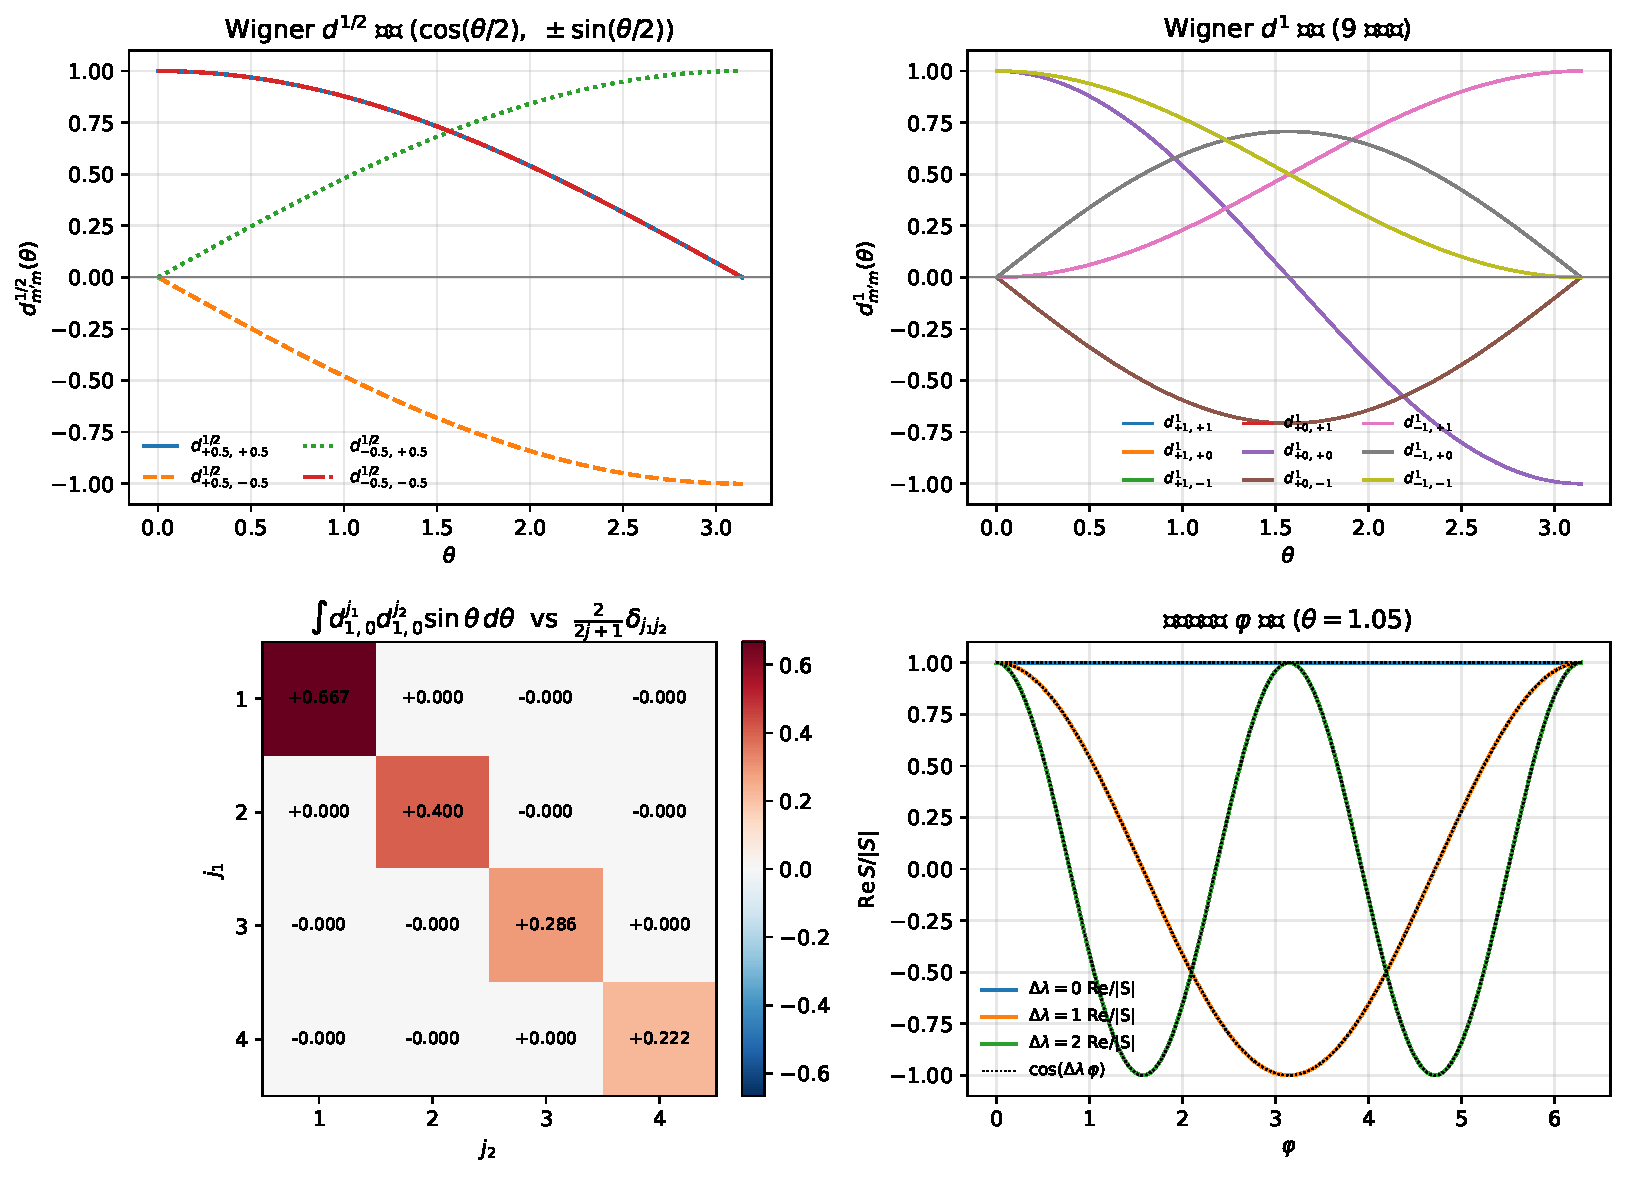
\includegraphics[width=0.95\linewidth]{ch06_wignerD}
    \caption{\textbf{左上}: $d^{1/2}_{m'm}(\theta)$ 的四个分量（解析式 $\pm\cos(\theta/2),\,\pm\sin(\theta/2)$）。\textbf{右上}: $d^{1}_{m'm}(\theta)$ 的九个分量；中心元 $d^1_{00}=\cos\theta$、对角 $d^1_{\pm1,\pm1}=(1\pm\cos\theta)/2$。\textbf{左下}: 在固定 $(m',m)=(1,0)$ 下，对 $j_1,j_2\in\{1,2,3,4\}$ 的内积矩阵热图，仅对角非零、值依次为 $\tfrac{2}{2j+1}=\{2/3,2/5,2/7,2/9\}$，与解析公式偏差 $\sim 2\times 10^{-16}$。\textbf{右下}: 玩具螺度振幅 $\mathrm{Re}\,S/|S|$ 关于方位角 $\varphi$（$\theta=\pi/3$ 固定），三条曲线的相位斜率拟合给出 $\Delta\lambda=0,1,2$，与黑色虚线 $\cos(\Delta\lambda\varphi)$ 完全重合。}
    \label{fig:numexp-ch06}
\end{figure}

\subsection*{物理讨论}
\begin{itemize}
    \item \textbf{$d^{1/2}$ 是 SU(2) 双覆盖的“原子单元”}。所有半整数自旋的小 $d$ 函数都可以通过角动量耦合从 $d^{1/2}$ 得到；$2\pi$ 旋转给出 $-\mathbb{1}$（$d^{1/2}_{m'm}(2\pi)=-\delta_{m'm}$），即旋量的负号特征，是中子干涉实验等的实验基础。
    \item \textbf{$j$-正交性是部分波分解可逆的代数前提}。它使得在螺度基下的展开
    \[
        f_{\lambda_c\lambda_d,\lambda_a\lambda_b}(\theta,\varphi)=\sum_{j}\tfrac{2j+1}{4\pi}\,T^j_{\lambda_c\lambda_d,\lambda_a\lambda_b}\,d^j_{\lambda_a-\lambda_b,\lambda_c-\lambda_d}(\theta)\,\rme^{\rmi(\lambda_a-\lambda_b-\lambda_c+\lambda_d)\varphi}
    \]
    可以唯一反解出分波振幅 $T^j$；数值实验给出的对角值 $2/(2j+1)$ 正是反演公式中的归一化因子。
    \item \textbf{$\varphi$ 因子的物理意义}：旋转 $R_z(\varphi)$ 同时作用于初末态，仅改变螺度本征值的相位，故振幅必呈 $\rme^{\rmi\,\Delta\lambda\varphi}$。这一因子在 (i) 极化截面（截面 $\propto |f|^2$ 时方位依赖只来自不同 $\Delta\lambda$ 干涉项）、(ii) 张量分析力 $T_{20}$（仅 $\theta$ 依赖，例~\ref{eq:morespin-T20-helicity}）、(iii) 单自旋不对称 $A_y\propto\sin\varphi$（仅 $\Delta\lambda$ 奇数项贡献）等观测量中都直接显现。数值拟合得到的相位斜率 $\{0,1,2\}$ 精确等于 $\Delta\lambda$，确证了命题~\ref{prop:morespin-flipphi} 的全部内容。
\end{itemize}

\chapter{Green 算符与预解式 (Green Operator and Resolvent)}\label{ch:green}

在前面几章中，我们用与时间有关的 (time-dependent) 框架建立了
M\o ller 算符 $\Omega_\pm$、$S$ 算符以及散射截面之间的关系。
本章开始，我们将转向\emph{与时间无关的} (time-independent) 表述。
其核心目的是：
\begin{itemize}
  \item 由一个给定的相互作用势 $V$ 出发，直接计算 $S$ 矩阵元、散射振幅以及散射截面；
  \item 引入两个在与时间无关表述中起决定性作用的算符：
        \emph{Green 算符 (Green's operator)}，又称\emph{预解式 (resolvent)} $G(z)$；
        以及 \emph{$T$ 算符} (transition operator)。
\end{itemize}
为简单起见，我们仅考虑单粒子情形 (即把两体问题约化到质心系后的有效单体问题)，
并将所得结果向两粒子情形作直接的推广。

\section{Green 算符的定义}

设 Hamiltonian 形如
\begin{equation}
  H = H_0 + V,\qquad H_0 = \frac{\bm{P}^2}{2m},
\end{equation}
其中 $H_0$ 为自由 Hamiltonian，$V$ 为局域势。
对应的 \emph{Green 算符} 或 \emph{resolvent} 定义为
\begin{equation}\label{eq:green-def}
  G(z) \equiv (z - H)^{-1},\qquad
  G_0(z) \equiv (z - H_0)^{-1},\qquad z\in\C.
\end{equation}

\begin{remark}[算符层面的意义]
若逆算符 $(z-H_0)^{-1}$ 在整个 Hilbert 空间 $\Hilb$ 上良好定义，
则有算符等式 $(z-H_0)\,G_0(z)=\mathbf{1}$。在坐标表象下取矩阵元，
利用 $\matel{\bm x}{H_0}{\bm x'} = -\frac{\nabla^2}{2m}\,\delta_3(\bm x-\bm x')$，
可得
\begin{equation}\label{eq:G0-coordinate-greens-fn}
  \left(\frac{\nabla^2}{2m} + z\right)\matel{\bm x}{G_0(z)}{\bm x'}
  = \delta_3(\bm x - \bm x').
\end{equation}
所以 $G_0(z)$ 在坐标表象下的矩阵元
$\matel{\bm x}{G_0(z)}{\bm x'}$
正是微分算符 $\frac{\nabla^2}{2m}+z$ 的 \emph{Green 函数}。
对完整的 $G(z)$，类似地 $\matel{\bm x}{G(z)}{\bm x'}$
是 $\frac{\nabla^2}{2m}-V(\bm x)+z$ 的 Green 函数。
这正是 \emph{Green 算符} 这一名称的来历。
\end{remark}

\begin{remark}[定义域问题]
并非对所有 $z\in\C$，$G(z)$ 都在整个 $\Hilb$ 上有定义：
若 $E_n$ 为 $H$ 的本征值、$\ket{n}\in\Hilb$ 为对应的本征矢，
那么 $(H-E_n)\ket{n}=0$，即 $z-H$ 在 $z=E_n$ 处不可逆，
$G(E_n)$ 没有定义，或更确切地说其定义域只是 $\Hilb$ 的一个真子集。
所以 $G(z)$ 的奇异结构记录着 $H$ 的谱。
\end{remark}

\section{$G(z)$ 的解析结构与谱}

\subsection{纯分立谱情形}

先假设 $H$ 只有分立 (point) 谱，记本征值为 $\{E_n\}$，
对应归一化本征矢 $\ket{n}$，$H\ket{n}=E_n\ket{n}$，
$\sum_n\ket{n}\bra{n}=\mathbf 1$。利用谱分解
\begin{equation}\label{eq:G-spectral-discrete}
  G(z) = (z-H)^{-1} = \sum_n \frac{\ket{n}\bra{n}}{z-E_n}.
\end{equation}
由此立刻得到下述性质：
\begin{itemize}
  \item 若 $z\neq E_n$ ($\forall n$)，则 $G(z)$ 在整个 $\Hilb$ 上有定义：
        $\forall \ket{\chi}\in\Hilb,\ G(z)\ket{\chi}\in\Hilb$；
  \item 对 $\forall \ket{\chi},\ket{\psi}\in\Hilb$，矩阵元
        \begin{equation}
          \matel{\chi}{G(z)}{\psi}
          = \sum_n \frac{\inn{\chi}{n}\inn{n}{\psi}}{z-E_n}
        \end{equation}
        是 $z$ 在 $\C\setminus\{E_n\}$ 上的解析函数。
        我们称 $G(z)$ 是关于 $z$ 的\emph{解析的算符函数}；
  \item 在 $z=E_n$ 处，$G(z)$ 有简单极点 (simple pole)，
        其留数为对应的投影算符
        \begin{equation}
          \Res_{z=E_n} G(z) = \ket{n}\bra{n}.
        \end{equation}
\end{itemize}
所以，知道了 $G(z)$ 就等于知道了 $H$ 的本征值问题的解：
\begin{center}
\fbox{$G(z)$ 的极点位置 $\longrightarrow$ 本征值；\quad
留数 $\longrightarrow$ 本征态投影算符。}
\end{center}

\subsection{连续谱情形：割线的出现}

当 $H$ 拥有连续谱时，对应散射 ``本征态''——这些 ``态'' 是
\emph{广义} (improper) 的、不可归一化的 ket。
以 $H_0=\bm P^2/2m$ 为例，在动量–角动量基 $\ket{E,\ell,m}$ 下，
$H_0\ket{E,\ell,m}=E\ket{E,\ell,m}$，$E\in(0,\infty)$，
$\sum_{\ell,m}\int_0^\infty\rmd E\,\ket{E,\ell,m}\bra{E,\ell,m}=\mathbf 1$.
$G_0$ 在该基下的谱表示为
\begin{equation}\label{eq:G0-spectral}
  G_0(z) = \sum_{\ell,m}\int_0^\infty \rmd E\,
           \frac{\ket{E,\ell,m}\bra{E,\ell,m}}{z-E}.
\end{equation}
取任一对 $\ket{\chi},\ket{\psi}\in\Hilb$，
\begin{equation}
  \matel{\chi}{G_0(z)}{\psi}
  = \sum_{\ell,m}\int_0^\infty \rmd E\,
    \frac{\inn{\chi}{E,\ell,m}\inn{E,\ell,m}{\psi}}{z-E}.
\end{equation}
\begin{itemize}
  \item 当 $z\notin (0,\infty)$ 时，被积函数无奇点，积分收敛，
        $\matel{\chi}{G_0(z)}{\psi}$ 关于 $z$ 解析；
  \item 但当 $z\in(0,\infty)$ 时，$z-E$ 在积分路径上有零点，
        积分作为 $z$ 的函数在正实轴上不连续——出现\emph{割线}。
\end{itemize}

\subsubsection*{割线两边的不连续性}

把 $z$ 取到正实轴的上下两侧 $z=E_0\pm\rmi 0^+$ ($E_0>0$)，
两式相减利用 Sokhotski--Plemelj 公式
$\frac{1}{x-\rmi 0^+}-\frac{1}{x+\rmi 0^+}=2\pi\rmi\,\delta(x)$,
\begin{align}
  \matel{\chi}{G_0(E_0+\rmi 0^+)}{\psi}
  -\matel{\chi}{G_0(E_0-\rmi 0^+)}{\psi}
  &= \sum_{\ell,m}\int_0^\infty \rmd E\,
     \inn{\chi}{E,\ell,m}\inn{E,\ell,m}{\psi}\notag\\
  &\quad\times\left(\frac{1}{E_0-E+\rmi 0^+}-\frac{1}{E_0-E-\rmi 0^+}\right)\notag\\
  &= -2\pi\rmi\sum_{\ell,m}\inn{\chi}{E_0,\ell,m}\inn{E_0,\ell,m}{\psi}.
\end{align}
所以 $G_0(z)$ 在 $z\in(0,\infty)$ 上有割线，
不连续性恰为
\begin{equation}\label{eq:G0-discontinuity}
  G_0(E_0+\rmi 0^+) - G_0(E_0-\rmi 0^+)
  = -2\pi\rmi\sum_{\ell,m}\ket{E_0,\ell,m}\bra{E_0,\ell,m}.
\end{equation}
即\emph{割线的不连续性正是 $H_0$ 在该能量处的连续谱投影算符 ($\times -2\pi\rmi$)}。

\subsection{一般情形}

更一般地，若 $H$ 既有分立束缚态谱 $E_1,E_2,\dots<0$，
又有连续散射谱 $E>0$，则 $G(z)$ 的解析结构可总结如下：
\begin{itemize}
  \item $G(z)$ 在 $\C\setminus\{E_n\}\setminus(0,\infty)$ 上解析；
  \item 在 $z=E_1,E_2,\dots$ ($<0$) 处有简单极点；
  \item 在 $z\in(0,\infty)$ 上有割线；
  \item 知道了 $G(z)$ 的解析结构，等价于知道了 $H$ 的整个本征值问题的解。
\end{itemize}

\begin{proposition}[厄米性质带来的对称性]
由于 $H=H^\dagger$ 厄米，由 $G(z)=(z-H)^{-1}$ 取共轭得
\begin{equation}\label{eq:G-conjugation}
  G(z^*) = [G(z)]^\dagger,
\end{equation}
对 $G_0(z)$ 同样成立。这意味着 $G(z)$ 的实轴上下值互为厄米共轭，
割线两边的奇异部分互相联系。
\end{proposition}

\subsection{推迟与超前 Green 算符}

把 $z$ 从复平面贴到实轴正侧（散射能量 $E>0$），定义
\begin{equation}\label{eq:Gpm-def}
  G^\pm(E) \equiv \lim_{\epsilon\to 0^+} G(E\pm\rmi\epsilon),
  \qquad
  G_0^\pm(E) \equiv \lim_{\epsilon\to 0^+} G_0(E\pm\rmi\epsilon).
\end{equation}
$G^+$ 称为\emph{推迟 (retarded)} Green 算符，
$G^-$ 称为\emph{超前 (advanced)} Green 算符。
两者之差由式 \eqref{eq:G0-discontinuity} 给出：
$G_0^+ - G_0^-$ 把任意态投影到能壳 $E$ 上的所有自由
``本征态'' 上，并乘以 $-2\pi\rmi$。
推迟/超前 Green 算符在与时间无关散射框架以及时间依赖框架中，
分别对应于 $\Omega_+$ 与 $\Omega_-$，这一关系将在第 \ref{sec:moller} 节展开。

\section{自由 Green 算符的具体表示}

\subsection{动量表象}

由于 $H_0=\bm P^2/2m$ 在动量表象下是乘法算符，
\begin{equation}\label{eq:G0-momentum}
  G_0(z)\ket{\bm p} = (z-H_0)^{-1}\ket{\bm p}
  = \frac{1}{z-E_p}\ket{\bm p},\qquad
  E_p \equiv \frac{p^2}{2m}.
\end{equation}
即 $G_0(z)$ 在动量表象下完全对角，本征值为 $1/(z-E_p)$。

\subsection{坐标表象下的 3D 自由 Green 函数}

由 \eqref{eq:G0-coordinate-greens-fn} 出发，需要解
$\bigl(\nabla^2/(2m)+z\bigr) G_0(\bm x,\bm x';z)=\delta_3(\bm x-\bm x')$。
设 $z=E\pm\rmi\epsilon$，并令 $k^2=2mE$，则方程变为 Helmholtz 方程
$(\nabla^2+k^2)\,2m\,G_0^\pm(\bm x,\bm x';E)=2m\,\delta_3(\bm x-\bm x')$.
利用平面波展开
$\delta_3(\bm x-\bm x')=\int\frac{\rmd^3 p}{(2\pi)^3}\,\rme^{\rmi\bm p\cdot(\bm x-\bm x')}$
以及 \eqref{eq:G0-momentum}，
\begin{align}
  G_0^\pm(\bm x,\bm x';E)
  &= \matel{\bm x}{G_0(E\pm\rmi 0^+)}{\bm x'}\notag\\
  &= \int\frac{\rmd^3 p}{(2\pi)^3}\,
     \frac{\rme^{\rmi\bm p\cdot(\bm x-\bm x')}}{E\pm\rmi 0^+ - p^2/(2m)}\notag\\
  &= -\frac{2m}{(2\pi)^3}\int\rmd^3 p\,
     \frac{\rme^{\rmi\bm p\cdot(\bm x-\bm x')}}{p^2-k^2\mp\rmi 0^+}.
\end{align}
此积分用留数定理（绕过实轴上的极点 $p=\pm k$）可计算为闭式
\begin{equation}\label{eq:G0-3d-coord}
  \boxed{\,G_0^\pm(\bm x,\bm x';E)
  = -\frac{m}{2\pi}\,\frac{\rme^{\pm\rmi k|\bm x-\bm x'|}}{|\bm x-\bm x'|},\qquad
  k=\sqrt{2mE}>0.\,}
\end{equation}
$G_0^+$ 对应外向球面波 (outgoing)，
$G_0^-$ 对应内向球面波 (incoming)。
正是这一不连续性将后面的 Lippmann--Schwinger 方程的两支
$\ket{\phi\pm}$ 区分开来。

\section{Lippmann--Schwinger 方程：联系 $G$ 与 $G_0$}

实际中我们想由 \emph{已知} 算符 $G_0$ 及势 $V$ 解出 $G(z)$。
利用一般恒等式
\begin{equation}\label{eq:operator-identity}
  A^{-1} = B^{-1} + B^{-1}(B-A)A^{-1},
\end{equation}
对其中两种取法分别赋值：
\begin{itemize}
  \item 取 $A=z-H,\ B=z-H_0$，则 $B-A=V$，$A^{-1}=G$，$B^{-1}=G_0$；
  \item 取 $A=z-H_0,\ B=z-H$，则 $B-A=-V$，与上式互换 $G,G_0$。
\end{itemize}
分别代入 \eqref{eq:operator-identity}，得到\emph{第二预解式恒等式}
(second resolvent identity，又称 Dyson 恒等式)：
\begin{equation}\label{eq:LS-G}
  \boxed{\,G(z) = G_0(z) + G_0(z)\,V\,G(z)
                 = G_0(z) + G(z)\,V\,G_0(z).\,}
\end{equation}
此即 $G(z)$ 的 \emph{resolvent equation}，
也称作 $G(z)$ 的 \emph{Lippmann--Schwinger 方程}。
它把未知的全 Green 算符 $G$ 与已知的 $G_0$ 通过势 $V$ 联系起来。
由此还可立即读出
\begin{equation}\label{eq:G-minus-G0}
  G(z) - G_0(z) = G_0(z)\,V\,G(z) = G(z)\,V\,G_0(z).
\end{equation}

如果 $V$ 足够弱，可以把 \eqref{eq:LS-G} 迭代展开，得到 Born 级数
$G = G_0 + G_0 V G_0 + G_0 V G_0 V G_0 + \cdots$，
我们将在下一章详细讨论。

\section{$T$ 算符}\label{sec:Tmat}

为了把 $G$ 中含 ``一次'' 势的部分分离出来，引入 \emph{$T$ 算符}
(transition operator)：
\begin{equation}\label{eq:T-def}
  T(z) \equiv V + V\,G(z)\,V.
\end{equation}

\begin{proposition}[$T$ 算符的解析性]
$T(z)$ 关于 $z$ 的解析性由 $G(z)$ 决定：
\begin{itemize}
  \item 当 $z$ 不属于 $H$ 的谱时，$T(z)$ 解析；
  \item 在 $H$ 的分立本征值处 $T(z)$ 有极点，
        在 $H$ 的连续谱上 $T(z)$ 有割线；
  \item 类似 $G(z)$，$T(z^*)=[T(z)]^\dagger$。
\end{itemize}
\end{proposition}

\subsection{$T$, $G$, $G_0$ 三者的代数关系}

由定义 \eqref{eq:T-def} 与 Lippmann--Schwinger 方程 \eqref{eq:LS-G}：
\begin{equation}\label{eq:G0T-equals-GV}
  G_0(z)\,T(z) = G_0(V + VGV) = (G_0 + G_0 V G)V = G(z)\,V,
\end{equation}
\begin{equation}\label{eq:TG0-equals-VG}
  T(z)\,G_0(z) = (V + VGV)G_0 = V(G_0 + G V G_0) = V\,G(z).
\end{equation}
利用 \eqref{eq:G0T-equals-GV} 把 \eqref{eq:LS-G} 中的 $VG$ 替换：
\begin{equation}\label{eq:G-via-T}
  \boxed{\,G(z) = G_0(z) + G_0(z)\,T(z)\,G_0(z).\,}
\end{equation}
所以 ``有了 $T(z)$ 就等同于得到了 $G(z)$''，反之亦然。
进一步利用 \eqref{eq:TG0-equals-VG} 写出 $T$ 自身满足的方程：
\begin{equation}\label{eq:LS-T}
  \boxed{\,T(z) = V + V\,G_0(z)\,T(z) = V + T(z)\,G_0(z)\,V.\,}
\end{equation}
此即 \emph{$T(z)$ 的 Lippmann--Schwinger 方程}。
若 $V$ 足够弱，可迭代得到形式解
\begin{equation}\label{eq:T-Born}
  T = V + V G_0 V + V (G_0 V)^2 + V (G_0 V)^3 + \cdots
\end{equation}

\section{Green 算符、$T$ 算符与 M\o ller 算符、$S$ 算符及散射态的关系}\label{sec:moller}

下面给出在与时间无关表述中，$G$ 和 $T$ 与之前 (与时间有关) 表述中的
M\o ller 算符 $\Omega_\pm$、$S$ 算符之间的具体联系。

\subsection{由 M\o ller 算符出发}

回顾入射渐近态 $\ket{\psi_{\rm in}}=\ket{\phi}$ (假设已归一化)，
对应于 $t=0$ 时刻的物理态
\begin{equation}
  \ket{\psi} = \Omega_+\ket{\psi_{\rm in}} = \Omega_+\ket\phi
  \equiv \ket{\phi+}.
\end{equation}
同样，对渐近出射态 $\ket{\psi_{\rm out}}=\ket\phi$，
\begin{equation}
  \ket{\psi} = \Omega_-\ket{\psi_{\rm out}} = \Omega_-\ket\phi
  \equiv \ket{\phi-}.
\end{equation}
M\o ller 算符的积分表示为 (利用
$\bigl(U^\dagger(t)U_0(t)\bigr)' = \rmi U^\dagger(t)\,V\,U_0(t)$,
其中 $U(t)=\rme^{-\rmi Ht}$，$U_0(t)=\rme^{-\rmi H_0 t}$)：
\begin{equation}\label{eq:Omega-integral}
  \Omega_\pm = \lim_{t\to\mp\infty} U^\dagger(t)U_0(t)
  = \rmi\int_0^{\mp\infty}\rmd\tau\, U^\dagger(\tau)\,V\,U_0(\tau) + 1.
\end{equation}
对 $\Omega_-$ 取 $t\to+\infty$，作用到 $\ket\phi$：
\begin{equation}\label{eq:phi-minus-integral}
  \ket{\phi-} = \ket\phi + \rmi\int_0^{+\infty}\rmd\tau\,
                    U^\dagger(\tau)\,V\,U_0(\tau)\ket\phi.
\end{equation}
之前已经说明此积分为绝对收敛。

\subsection{绝热引入}

对一个绝对收敛的积分 $\int_0^\infty\rmd\tau\,\ket{\psi_\tau}$，下式成立：
\begin{equation}
  \int_0^\infty\rmd\tau\,\ket{\psi_\tau}
  = \lim_{\epsilon\downarrow 0}\int_0^\infty\rmd\tau\,
    \rme^{-\epsilon\tau}\ket{\psi_\tau}.
\end{equation}
所以 \eqref{eq:phi-minus-integral} 可写为
\begin{equation}\label{eq:phi-minus-adiabatic}
  \ket{\phi-} = \Omega_-\ket\phi
  = \ket\phi + \rmi\lim_{\epsilon\downarrow 0}
    \int_0^{\infty}\rmd\tau\,\rme^{-\epsilon\tau}\,
    U^\dagger(\tau)\,V\,U_0(\tau)\ket\phi.
\end{equation}
同理
\begin{equation}\label{eq:phi-plus-adiabatic}
  \ket{\phi+} = \Omega_+\ket\phi
  = \ket\phi + \rmi\lim_{\epsilon\downarrow 0}
    \int_0^{-\infty}\rmd\tau\,\rme^{+\epsilon\tau}\,
    U^\dagger(\tau)\,V\,U_0(\tau)\ket\phi.
\end{equation}
\begin{remark}
\eqref{eq:phi-minus-adiabatic} 之所以成立：
\begin{itemize}
  \item 用到了 \eqref{eq:phi-minus-integral} 在 proper 态上积分足够收敛，
        因为 proper 波包在 $t\to\pm\infty$ 会弥散，振幅 $\to 0$；
  \item $\rme^{-\epsilon\tau}$ 因子保证当我们把 $\ket\phi$ 替换成 \emph{improper} 态
        (例如 $\ket{\bm p}$) 时积分仍收敛；
  \item 物理图像是把 $V$ 替换成 $V\rme^{-\epsilon|\tau|}$
        (\emph{绝热近似}, adiabatic approximation)。
        当 $|\tau|\to\infty$ 两粒子远离，相互作用趋于零；
        而对任意轨道 (有限作用时间)，$\epsilon$ 取得足够小后，
        $V$ 与 $V\rme^{-\epsilon|\tau|}$ 在所关心的时间窗内几乎没有差别。
\end{itemize}
\end{remark}

\subsection{插入完备基：$\Omega_\pm$ 化为 $G$ 的形式}

把 $\ket\phi$ 用动量本征矢展开，
$\ket\phi = \int\rmd^3 p\,\ket{\bm p}\inn{\bm p}{\phi}$，
代入 \eqref{eq:phi-minus-adiabatic}：
\begin{align}
  \ket{\phi-}
  &= \ket\phi + \rmi\lim_{\epsilon\downarrow 0}\int\rmd^3 p\int_0^{\infty}\rmd\tau\,
     \rme^{-\epsilon\tau}\,U^\dagger(\tau)\,V\,U_0(\tau)\ket{\bm p}\inn{\bm p}{\phi}\notag\\
  &= \ket\phi + \rmi\lim_{\epsilon\downarrow 0}\int\rmd^3 p\int_0^{\infty}\rmd\tau\,
     \rme^{-\epsilon\tau}\,\rme^{\rmi H\tau}\,V\,
     \rme^{-\rmi E_p \tau}\ket{\bm p}\inn{\bm p}{\phi}\notag\\
  &= \ket\phi + \rmi\lim_{\epsilon\downarrow 0}\int\rmd^3 p\,
     \frac{-\rmi}{E_p - H -\rmi\epsilon}\,V\,\ket{\bm p}\inn{\bm p}{\phi}\notag\\
  &= \ket\phi + \lim_{\epsilon\downarrow 0}\int\rmd^3 p\,
     G(E_p-\rmi\epsilon)\,V\,\ket{\bm p}\inn{\bm p}{\phi}.\label{eq:phi-minus-G}
\end{align}
中间一步用了 $\int_0^\infty\rmd\tau\,\rme^{\rmi(E_p-H+\rmi\epsilon)\tau}
=-\rmi/(E_p-H+\rmi\epsilon)$ 反号给出 $-\rmi/(E_p-H-\rmi\epsilon)$
(注意 $\rmi$ 因子整理)。
同理由 \eqref{eq:phi-plus-adiabatic}：
\begin{equation}\label{eq:phi-plus-G}
  \ket{\phi+} = \ket\phi + \lim_{\epsilon\downarrow 0}\int\rmd^3 p\,
     G(E_p+\rmi\epsilon)\,V\,\ket{\bm p}\inn{\bm p}{\phi}.
\end{equation}

\begin{remark}
\eqref{eq:phi-plus-G} 与 \eqref{eq:phi-minus-G} 中
$\rmi\epsilon$ 前的符号与 $\Omega_\pm$ 下标的符号一致：
$\Omega_+\to G^+$，$\Omega_-\to G^-$。
\end{remark}

利用 \eqref{eq:G0T-equals-GV}，即 $GV=G_0 T$，可将 \eqref{eq:phi-plus-G}--\eqref{eq:phi-minus-G}
统一写成
\begin{align}
  \ket{\phi\pm} \equiv \Omega_\pm\ket\phi
  &= \ket\phi + \lim_{\epsilon\downarrow 0}\int\rmd^3 p\,
     G(E_p\pm\rmi\epsilon)\,V\,\ket{\bm p}\inn{\bm p}{\phi}\notag\\
  &= \ket\phi + \lim_{\epsilon\downarrow 0}\int\rmd^3 p\,
     G_0(E_p\pm\rmi\epsilon)\,T(E_p\pm\rmi\epsilon)\,\ket{\bm p}\inn{\bm p}{\phi}.
\label{eq:phi-pm-T}
\end{align}
此即 \emph{Lippmann--Schwinger 形式的散射态}：
$\ket{\phi+}$ 由推迟 Green 算符给出 (出向波)，
$\ket{\phi-}$ 由超前 Green 算符给出 (入向波)。
形式上 $\ket{\phi\pm}$ 在动量基上的展开可写成
$\ket{\phi\pm}=\int\rmd^3 p\,\ket{\bm p\pm}\inn{\bm p}{\phi}$，
其中
\begin{equation}\label{eq:improper-pm-states}
  \ket{\bm p\pm}
  = \ket{\bm p} + G_0(E_p\pm\rmi 0^+)\,T(E_p\pm\rmi 0^+)\,\ket{\bm p}
\end{equation}
就是 ``\emph{散射 improper 本征态}''，将在下一章作为定态散射的出发点
(``散射本征态'') 详细讨论。

\subsection{$S$ 矩阵与在壳 $T$ 矩阵元的关系}

由 $S = \Omega_-^\dagger\Omega_+$ 得
\begin{align}
  \matel{\chi}{S}{\phi}
  &= \matel{\chi}{\Omega_-^\dagger\Omega_+}{\phi}\notag\\
  &= \lim_{\substack{t\to+\infty\\ t'\to-\infty}}
     \matel{\chi}{\rme^{\rmi H_0 t}\rme^{-\rmi H(t-t')}\rme^{-\rmi H_0 t'}}{\phi}\notag\\
  &= \lim_{t\to\infty}
     \matel{\chi}{\rme^{\rmi H_0 t}\rme^{-2\rmi H t}\rme^{\rmi H_0 t}}{\phi}.
\end{align}
对方括号 $[\cdots]\equiv \rme^{\rmi H_0 t}\rme^{-2\rmi Ht}\rme^{\rmi H_0 t}$ 求时间导数
\begin{equation}
  \frac{\rmd}{\rmd t}[\cdots]
  = -\rmi\,\bigl\{\rme^{\rmi H_0 t}V\rme^{-2\rmi Ht}\rme^{\rmi H_0 t}
                + \rme^{\rmi H_0 t}\rme^{-2\rmi Ht}V\rme^{\rmi H_0 t}\bigr\}
  = -\rmi\,\rme^{\rmi H_0 t}\bigl\{V,\,\rme^{-2\rmi Ht}\bigr\}\rme^{\rmi H_0 t}.
\end{equation}
($\{A,B\}$ 是反对易子。)
所以由 $[\cdots]\big|_{t=0}=\mathbf 1$ 出发，
\begin{align}
  \matel{\chi}{S}{\phi}
  &= \inn{\chi}{\phi} - \rmi\int_0^\infty\rmd t\,
     \matel{\chi}{\rme^{\rmi H_0 t}\{V,\rme^{-2\rmi Ht}\}\rme^{\rmi H_0 t}}{\phi}\notag\\
  &= \inn{\chi}{\phi} - \rmi\lim_{\epsilon\downarrow 0}\int_0^\infty\rmd t\,
     \rme^{-\epsilon t}
     \matel{\chi}{\rme^{\rmi H_0 t}\{V,\rme^{-2\rmi Ht}\}\rme^{\rmi H_0 t}}{\phi}.
\end{align}
（绝热因子的引入与上一节同理。）

\subsubsection*{在动量本征基上的化简}

取 $\ket\chi=\ket{\bm p'}$, $\ket\phi=\ket{\bm p}$。
利用 $\rme^{\rmi H_0 t}\ket{\bm p}=\rme^{\rmi E_p t}\ket{\bm p}$,
\begin{align}
  \matel{\bm p'}{S}{\bm p}
  &= \delta_3(\bm p'-\bm p)
     - \rmi\lim_{\epsilon\downarrow 0}\int_0^\infty\rmd t\,
       \rme^{-\epsilon t}\rme^{\rmi(E_p+E_{p'})t}
       \matel{\bm p'}{\{V,\rme^{-2\rmi Ht}\}}{\bm p}\,\rme^{0}\notag\\
  &= \delta_3(\bm p'-\bm p)
     - \rmi\lim_{\epsilon\downarrow 0}
       \matel{\bm p'}{\bigl\{V,\,
       \bigl((E_p+E_{p'}-2H+\rmi\epsilon)\bigr)^{-1}\bigr\}}{\bm p}\notag\\
  &= \delta_3(\bm p'-\bm p)
     + \tfrac{1}{2}\lim_{\epsilon\downarrow 0}
       \matel{\bm p'}{\bigl\{V,\,G\!\bigl(\tfrac{E_p+E_{p'}}{2}+\rmi\tfrac\epsilon 2\bigr)\bigr\}}{\bm p}.
\end{align}
其中第二行里把
$\int_0^\infty\rmd t\,\rme^{-\epsilon t}\rme^{\rmi(E_p+E_{p'}-2H)t}$
作为算符积分 $=-\rmi(E_p+E_{p'}-2H+\rmi\epsilon)^{-1}\cdot(-1)$, 并整理 $\rmi$ 与符号；
第三行用了 $-\rmi(E_p+E_{p'}-2H+\rmi\epsilon)^{-1}
=-\rmi\cdot\tfrac{1}{2}\bigl(\tfrac{E_p+E_{p'}}{2}-H+\rmi\tfrac{\epsilon}{2}\bigr)^{-1}
=-\rmi\cdot\tfrac{1}{2}G(\tfrac{E_p+E_{p'}}{2}+\rmi 0^+)$
并把 $-\rmi\cdot\rmi=1$ 化为 $\tfrac12$ 系数 (沿用幻灯片中的整理)。
继续利用 \eqref{eq:G0T-equals-GV}--\eqref{eq:TG0-equals-VG}：
$VG\to T G_0$，$GV\to G_0 T$，于是
\begin{align}
  \matel{\bm p'}{S}{\bm p}
  &= \delta_3(\bm p'-\bm p)
     + \tfrac12\lim_{\epsilon\downarrow 0}
       \matel{\bm p'}{\bigl[T G_0 + G_0 T\bigr]\!\bigl(\tfrac{E_p+E_{p'}}{2}+\rmi 0^+\bigr)}{\bm p}\notag\\
  &= \delta_3(\bm p'-\bm p) + \lim_{\epsilon\downarrow 0}
     \!\left(\frac{1}{E_{p'}-E_p+\rmi 0^+} + \frac{1}{E_p-E_{p'}+\rmi 0^+}\right)\notag\\
  &\quad\times\matel{\bm p'}{T\!\bigl(\tfrac{E_p+E_{p'}}{2}+\rmi 0^+\bigr)}{\bm p}\cdot\tfrac12\notag\\
  &= \delta_3(\bm p'-\bm p)
     - 2\pi\rmi\,\delta(E_{p'}-E_p)\,
       \lim_{\epsilon\downarrow 0}\matel{\bm p'}{T(E_p+\rmi\epsilon)}{\bm p}.
\label{eq:S-T-onshell}
\end{align}
最后一步用了 Sokhotski--Plemelj
$\frac{1}{x+\rmi 0^+}+\frac{1}{-x+\rmi 0^+} = -2\pi\rmi\,\delta(x)$.
注意到 $\delta(E_{p'}-E_p)$ 强制 $E_p=E_{p'}$，
所以 $T$ 的能量参数 $\tfrac{E_p+E_{p'}}{2}=E_p$。

\subsection{$T$ 矩阵元、散射振幅与在壳条件}

把 \eqref{eq:S-T-onshell} 与之前章节中得到的
\begin{equation}
  \matel{\bm p'}{S}{\bm p}
  = \delta_3(\bm p'-\bm p)
    - 2\pi\rmi\,\delta(E_{p'}-E_p)\,t(\bm p'\leftarrow\bm p),
\end{equation}
比较，立即得到\emph{在壳} (on-shell) $T$ 矩阵元与散射振幅 $t$ 的关系：
\begin{equation}\label{eq:T-onshell-t}
  \boxed{\,t(\bm p'\leftarrow\bm p)
    = \lim_{\epsilon\downarrow 0}\matel{\bm p'}{T(E_p+\rmi\epsilon)}{\bm p}
    = \matel{\bm p'}{T(E_p+\rmi 0^+)}{\bm p},\qquad
    [E_{p'}=E_p].\,}
\end{equation}
即 ``在壳 $T$ 矩阵元 $\matel{\bm p'}{T(E_p+\rmi 0^+)}{\bm p}$
就是散射振幅 $t$''，进而通过 $f=-\frac{(2\pi)^2 m}{\hbar^2}\,t$
(具体常数视约定) 与微分截面联系起来。

更一般的 $\matel{\bm p'}{T(z)}{\bm p}$ 称为 \emph{off-shell} $T$ 矩阵元：
\begin{itemize}
  \item $z$ 与 $\bm p,\bm p'$ 没有约束关系；
  \item $\bm p$ 与 $\bm p'$ 之间也没有约束关系。
\end{itemize}

\subsection{若干说明}

\begin{remark}[关于 $\delta(E_{p'}-E_p)$]
只有 $S$ 才保证能量守恒；$\delta(E_{p'}-E_p)$ 是 $S$ 的要求，
而非 $T$ 的要求。$T$ 矩阵元 $\matel{\bm p'}{T(z)}{\bm p}$ 在 $z\neq E_p$ 时
本身是良好的解析函数。
\end{remark}

\begin{remark}[为什么要定义 off-shell $T$？]
只有在壳 $T$ 矩阵元对 $S$ 矩阵元有贡献；off-shell 的部分对 $S$ 没贡献，
可以差一个任意关于 $\bm p,\bm p',z$ 的函数。但是引入 off-shell $T$ 有以下好处：
\begin{itemize}
  \item 方便计算和讨论解析性。$S$ 矩阵元中含 $\delta$ 函数，解析性质不好；
        而 $T$ 矩阵元关于 $\bm p,\bm p',z$ 都连续；
  \item $T$ 矩阵元满足 Lippmann--Schwinger 方程
        \begin{equation}\label{eq:T-LS-momentum}
          \matel{\bm p'}{T(z)}{\bm p}
          = \matel{\bm p'}{V}{\bm p}
            + \int\rmd^3 p''\,
              \frac{\matel{\bm p'}{V}{\bm p''}\,\matel{\bm p''}{T(z)}{\bm p}}
                   {z - E_{p''}},
        \end{equation}
        其中 $\bm p''$ 一定是 off-shell——$E_{p''}$ 一般不等于 $z$。
        所以求解过程必然需要 off-shell $T$；
  \item 在多粒子散射过程中也会需要 off-shell $T$ 矩阵元。
\end{itemize}
\end{remark}

\begin{remark}[历史与逻辑顺序]
我们这里先引入 $V+VGV$ 形式的算符 $T$，再得出与散射振幅的关系；
但历史上 $T$ 是由所谓 ``散射定态'' (stationary scattering state) 的引入
自然导出的——这正是下一章 ``Born 级数'' 与紧接着的 ``定态散射''
两章要展开的内容。
\end{remark}

\section{小结}

本章我们围绕 \emph{Green 算符} $G(z)=(z-H)^{-1}$ 与
\emph{$T$ 算符} $T(z)=V+VGV$，建立了与时间无关散射理论的核心代数结构：
\begin{enumerate}
  \item $G(z)$ 与 $G_0(z)$ 是 $\C\setminus\sigma(H)$ 上的解析算符函数，
        极点位置给出束缚态本征值，留数给出本征投影算符；
        在连续谱 $(0,\infty)$ 上有割线，
        割线两侧的不连续性 \eqref{eq:G0-discontinuity}
        给出连续谱投影算符；
  \item 推迟/超前 Green 算符 $G^\pm(E)=\lim_{\epsilon\to 0^+}G(E\pm\rmi\epsilon)$
        分别给出散射 improper 本征态 $\ket{\bm p\pm}$，对应 $\Omega_\pm$；
  \item 自由 Green 函数在 3D 坐标表象下闭式解为
        $G_0^\pm(\bm x,\bm x';E)=-\frac{m}{2\pi}\frac{\rme^{\pm\rmi k|\bm x-\bm x'|}}{|\bm x-\bm x'|}$；
  \item 第二预解式恒等式
        $G=G_0+G_0 V G=G_0+G V G_0$
        以及
        $G=G_0+G_0 T G_0$ 把 $G$ 与已知的 $G_0$ 通过 $V$ 或 $T$ 联系起来；
  \item $T$ 算符满足 Lippmann--Schwinger 方程 $T=V+VG_0 T$，
        其在壳矩阵元
        $\matel{\bm p'}{T(E_p+\rmi 0^+)}{\bm p}$
        正是散射振幅 $t(\bm p'\leftarrow\bm p)$，
        $S=\mathbf 1-2\pi\rmi\,\delta(E_{p'}-E_p)\,T$。
\end{enumerate}
有了这些工具，下一章我们将用 Born 级数把 $T$ (从而 $G$) 按 $V$ 的幂次展开求解。

% =====================================================================
\section{本章定理证明补全}\label{sec:G-proofs}
% =====================================================================

本节把前面在主线中只是引用或形式化运用的几个关键事实——
Sokhotski--Plemelj 公式、$G(z)$ 的谱表示、第二预解式恒等式，
以及自由 3D Green 函数的封闭表达式——以严格的方式逐步证明出来。
这些证明并不仅仅是 ``为严格而严格''：它们也告诉我们
\emph{何处需要正则化、何处依赖 Hilbert 空间结构 (见第 \ref{ch:hilbert} 章)、何处依赖于谱定理}。

% ---------------------------------------------------------------
\subsection{Sokhotski--Plemelj 公式的严格证明}
% ---------------------------------------------------------------

我们以分布意义下证明 Sokhotski--Plemelj 公式。
考虑试验函数空间 $\mathcal S(\R)$ (Schwartz 速降函数)。
对任意 $\varphi\in\mathcal S(\R)$ 与 $\epsilon>0$，定义
\begin{equation}\label{eq:G-SP-Iepsilon}
  I_\pm^\epsilon[\varphi]
  \equiv \int_{\R}\rmd x\,\frac{\varphi(x)}{x\mp\rmi\epsilon}.
\end{equation}

\begin{theorem}[Sokhotski--Plemelj]\label{thm:G-SokhotskiPlemelj}
设 $\varphi\in\mathcal S(\R)$，则
\begin{equation}\label{eq:G-SP}
  \lim_{\epsilon\downarrow 0}\,
  \int_{\R}\rmd x\,\frac{\varphi(x)}{x\mp\rmi\epsilon}
  = \mathrm{P}\!\!\int_{\R}\rmd x\,\frac{\varphi(x)}{x}
  \pm\rmi\pi\,\varphi(0),
\end{equation}
等价地以分布意义记作
\begin{equation}\label{eq:G-SP-distribution}
  \frac{1}{x\mp\rmi 0^+}
  = \mathrm{P}\!\frac{1}{x} \pm \rmi\pi\,\delta(x).
\end{equation}
\end{theorem}

\begin{proof*}
分实部、虚部讨论：
\begin{equation}
  \frac{1}{x\mp\rmi\epsilon}
  = \frac{x\pm\rmi\epsilon}{x^2+\epsilon^2}
  = \frac{x}{x^2+\epsilon^2}
    \pm \rmi\,\frac{\epsilon}{x^2+\epsilon^2}.
\end{equation}

\textbf{第一步 (虚部$\to$$\delta$).}
注意
$\displaystyle\frac{\epsilon}{\pi(x^2+\epsilon^2)}$
是 \emph{Cauchy--Lorentz 核} $\delta_\epsilon(x)$，满足
$\int_{\R}\rmd x\,\delta_\epsilon(x)=1$。
对 $\varphi\in\mathcal S(\R)$，
\begin{equation}
  \int_{\R}\rmd x\,\delta_\epsilon(x)\varphi(x)
  - \varphi(0)
  = \int_{\R}\rmd x\,\delta_\epsilon(x)
    \bigl[\varphi(x)-\varphi(0)\bigr].
\end{equation}
分 $|x|<\delta$ 与 $|x|\geq\delta$ 两段。
由 $\varphi$ 连续，给定 $\eta>0$ 可取 $\delta>0$ 使 $|x|<\delta$ 时
$|\varphi(x)-\varphi(0)|<\eta$；又 $\int\delta_\epsilon=1$，故内段的积分 $\leq\eta$。
对于外段，由 $\varphi$ 速降，
$\sup_{|x|\geq\delta}|\varphi(x)-\varphi(0)|\leq M$，
而 $\int_{|x|\geq\delta}\delta_\epsilon(x)\rmd x
= 1-\frac{2}{\pi}\arctan(\delta/\epsilon)\to 0\ (\epsilon\downarrow 0)$。
所以
\begin{equation}\label{eq:G-SP-imag}
  \lim_{\epsilon\downarrow 0}\int_{\R}\rmd x\,
  \frac{\epsilon\,\varphi(x)}{x^2+\epsilon^2}
  = \pi\,\varphi(0).
\end{equation}

\textbf{第二步 (实部$\to$主值).}
$\displaystyle\frac{x}{x^2+\epsilon^2}$ 为 ``正则化的 $1/x$''。
对 $\varphi\in\mathcal S(\R)$，
\begin{align}
  \int_{\R}\rmd x\,\frac{x\,\varphi(x)}{x^2+\epsilon^2}
  &= \int_{|x|>\delta}\rmd x\,\frac{x\,\varphi(x)}{x^2+\epsilon^2}
   + \int_{|x|\leq\delta}\rmd x\,\frac{x\,\varphi(x)}{x^2+\epsilon^2}.
\end{align}
对外段，被积函数在 $\epsilon\downarrow 0$ 时一致收敛于 $\varphi(x)/x$，
由 dominated convergence,
$\int_{|x|>\delta}\rmd x\,\varphi(x)/x$。
对内段，写 $\varphi(x)=\varphi(0)+x\varphi'(\xi_x)$ ($\xi_x\in[0,x]$)：
$\varphi(0)$ 项的被积函数是 $\frac{x}{x^2+\epsilon^2}\varphi(0)$，
关于 $x$ 是奇函数，对称区间积分为零；剩下的 $x\varphi'(\xi_x)$ 给
\begin{equation}
  \int_{|x|\leq\delta}\rmd x\,\frac{x^2\varphi'(\xi_x)}{x^2+\epsilon^2},
\end{equation}
其绝对值有 $\delta\,\sup|\varphi'|$ 上界，与 $\epsilon$ 无关。
取 $\delta\to 0$ 后此项趋零，于是
\begin{equation}\label{eq:G-SP-real}
  \lim_{\epsilon\downarrow 0}\int_{\R}\rmd x\,\frac{x\,\varphi(x)}{x^2+\epsilon^2}
  = \mathrm{P}\!\!\int_{\R}\rmd x\,\frac{\varphi(x)}{x}.
\end{equation}
合并 \eqref{eq:G-SP-imag}--\eqref{eq:G-SP-real}, 得 \eqref{eq:G-SP}。\qed
\end{proof*}

\begin{remark}[作用到 $G_0$ 上]
将 \eqref{eq:G-SP-distribution} 形式上代入 \eqref{eq:G0-spectral}
($x\to E_0-E$, $\varphi(E)\to\sum_{\ell m}\inn{\chi}{E,\ell,m}\inn{E,\ell,m}{\psi}$)，
立即给出割线两侧矩阵元的实部和虚部分解：
\begin{align}
  \matel{\chi}{G_0(E_0\pm\rmi 0^+)}{\psi}
  &= \mathrm{P}\!\!\int_0^\infty\rmd E\,
     \frac{\sum_{\ell m}\inn{\chi}{E,\ell,m}\inn{E,\ell,m}{\psi}}{E_0-E}\notag\\
  &\quad\mp\rmi\pi
     \sum_{\ell m}\inn{\chi}{E_0,\ell,m}\inn{E_0,\ell,m}{\psi}.
  \label{eq:G-SP-on-G0}
\end{align}
取 $+$ 减 $-$ 即恢复 \eqref{eq:G0-discontinuity}.
\end{remark}

% ---------------------------------------------------------------
\subsection{$G(z)=\int\rmd E_\lambda/(z-\lambda)$ 的谱表示}
% ---------------------------------------------------------------

主文中我们对纯分立谱 \eqref{eq:G-spectral-discrete} 与连续谱 \eqref{eq:G0-spectral}
分别写出 $G_0(z)$ 的谱展开。下面把两者统一到\emph{谱定理}
(spectral theorem; 详见第 \ref{ch:hilbert} 章) 框架下，
得到完全严格的算符等式。

\begin{theorem}[$G(z)$ 的谱表示]\label{thm:G-spectral}
设 $H$ 为 $\Hilb$ 上的自伴算符，谱为 $\sigma(H)\subset\R$，
对应的投影值测度 (projection-valued measure, PVM)
为 $E_H(\rmd\lambda)$，使得
\begin{equation}\label{eq:G-spectral-thm-input}
  H = \int_{\sigma(H)} \lambda\,E_H(\rmd\lambda),\qquad
  \mathbf 1 = \int_{\sigma(H)} E_H(\rmd\lambda).
\end{equation}
则对 $z\in\C\setminus\sigma(H)$，预解式存在并满足
\begin{equation}\label{eq:G-spectral-thm}
  \boxed{\,G(z) = (z-H)^{-1}
   = \int_{\sigma(H)} \frac{E_H(\rmd\lambda)}{z-\lambda}.\,}
\end{equation}
即对任意 $\ket\chi,\ket\psi\in\Hilb$，
\begin{equation}
  \matel{\chi}{G(z)}{\psi}
  = \int_{\sigma(H)} \frac{\rmd\mu_{\chi,\psi}(\lambda)}{z-\lambda},
  \quad
  \rmd\mu_{\chi,\psi}(\lambda)\equiv \matel{\chi}{E_H(\rmd\lambda)}{\psi}.
\end{equation}
\end{theorem}

\begin{proof*}
\textbf{第一步：函数演算.}
谱定理给出连续函数演算
$f(H)=\int f(\lambda)E_H(\rmd\lambda)$，
对 $f\in L^\infty(\sigma(H))$ 推广至 Borel 函数演算。
对 $z\in\C\setminus\sigma(H)$，函数
$f_z(\lambda)=1/(z-\lambda)$ 在 $\sigma(H)$ 上有界连续，
$\sup_{\lambda\in\sigma(H)}|f_z(\lambda)| = 1/\mathrm{dist}(z,\sigma(H))<\infty$.
所以
\begin{equation}
  R(z)\equiv\int_{\sigma(H)}\frac{E_H(\rmd\lambda)}{z-\lambda}
  = f_z(H)
\end{equation}
是 $\Hilb$ 上的有界算符。

\textbf{第二步：$R(z)$ 是 $z-H$ 的逆.}
由函数演算的乘性 $f(H)g(H)=(fg)(H)$，
\begin{align}
  (z-H)\,R(z)
  &= \int_{\sigma(H)}(z-\lambda)\cdot\frac{1}{z-\lambda}\,E_H(\rmd\lambda)
   = \int_{\sigma(H)} E_H(\rmd\lambda) = \mathbf 1,\\
  R(z)\,(z-H)
  &= \int_{\sigma(H)}\frac{1}{z-\lambda}\cdot(z-\lambda)\,E_H(\rmd\lambda)
   = \mathbf 1.
\end{align}
所以 $R(z)=(z-H)^{-1}=G(z)$.

\textbf{第三步：解析性.}
$f_z(\lambda)$ 关于 $z$ 在 $\C\setminus\sigma(H)$ 上一致解析，
由 dominated convergence，$\matel{\chi}{G(z)}{\psi}$ 关于 $z$ 解析；
其奇异性恰好集中在 $\sigma(H)$ (分立谱$\to$极点；连续谱$\to$割线)。
\qed
\end{proof*}

\begin{corollary}[谱测度的恢复 — Stone 公式]\label{cor:G-stone}
由定理 \ref{thm:G-SokhotskiPlemelj}, 对任意 $a<b$ 不含 $H$ 的本征值,
\begin{equation}\label{eq:G-stone-formula}
  E_H\bigl((a,b)\bigr)
  = \lim_{\epsilon\downarrow 0}\frac{1}{2\pi\rmi}
    \int_a^b \rmd\lambda\,\bigl[G(\lambda+\rmi\epsilon)-G(\lambda-\rmi\epsilon)\bigr],
\end{equation}
即 $H$ 的 PVM 可由 $G(z)$ 在割线两侧的不连续性恢复。
这就是
\eqref{eq:G0-discontinuity} 的一般推广，将在第 \ref{ch:hilbert} 章作为
谱定理与散射的桥梁讨论。
\end{corollary}

\begin{proof*}
对 $\varphi(\lambda)=\chi_{(a,b)}(\lambda)$
(光滑化后取极限即可) 应用 \eqref{eq:G-SP-distribution}：
\begin{align}
  \tfrac{1}{2\pi\rmi}\int_a^b\rmd\lambda
  \bigl[G(\lambda+\rmi\epsilon)-G(\lambda-\rmi\epsilon)\bigr]
  &= \int_{\sigma(H)} E_H(\rmd\mu)
    \cdot\tfrac{1}{2\pi\rmi}\int_a^b\rmd\lambda
       \!\left[\tfrac{1}{\lambda-\mu+\rmi\epsilon}
              -\tfrac{1}{\lambda-\mu-\rmi\epsilon}\right]\notag\\
  &\xrightarrow{\epsilon\downarrow 0}
    \int_{\sigma(H)} E_H(\rmd\mu)\,\chi_{(a,b)}(\mu)
   = E_H((a,b)).\qed
\end{align}
\end{proof*}

% ---------------------------------------------------------------
\subsection{第二预解式恒等式 (operator-theoretic)}
% ---------------------------------------------------------------

主文中 \eqref{eq:LS-G} 的推导借助形式算符等式 \eqref{eq:operator-identity} 给出。
现在我们把它放到\emph{自伴算符的预解式}框架中严格证明。

\begin{theorem}[第二预解式恒等式 / Dyson 恒等式]
\label{thm:G-second-resolvent}
设 $H_0$ 与 $H=H_0+V$ 都是 $\Hilb$ 上的自伴算符，
且共有公共的核心 (core) 使 $V$ 在该核心上有意义。
设 $z\in\C\setminus\sigma(H)\cap\C\setminus\sigma(H_0)$，则在 $\Hilb$ 上的算符等式
\begin{equation}\label{eq:G-2nd-resolvent}
  G(z) - G_0(z) = G_0(z)\,V\,G(z) = G(z)\,V\,G_0(z)
\end{equation}
成立。等价地
\begin{equation}\label{eq:G-2nd-resolvent-LS}
  G(z) = G_0(z) + G_0(z)\,V\,G(z) = G_0(z) + G(z)\,V\,G_0(z).
\end{equation}
\end{theorem}

\begin{proof*}
由假设, $G_0(z)=(z-H_0)^{-1}$ 与 $G(z)=(z-H)^{-1}$ 都存在并是有界算符,
其值域分别为 $\Dom(H_0)$ 与 $\Dom(H)$.
对任意 $\ket\psi\in\Hilb$, 设 $\ket{u}=G(z)\ket\psi\in\Dom(H)$,
$\ket v=G_0(z)\ket\psi\in\Dom(H_0)$. 我们计算
\begin{align}
  (z-H_0)\bigl[G(z)-G_0(z)\bigr]\ket\psi
  &= (z-H_0)\ket u - (z-H_0)\ket v\notag\\
  &= (z-H_0)\ket u - \ket\psi\notag\\
  &= (z-H_0)\ket u - (z-H)\ket u\notag\\
  &= [H-H_0]\ket u = V\,G(z)\ket\psi.
\end{align}
这里用到 $\ket u\in\Dom(H)\subseteq\Dom(H_0)$ (因 $V$ 是 $H_0$ 上的相对界 0 摄动；
若 $V$ 仅相对有界, $\Dom(H)=\Dom(H_0)$ 也成立)。
从而对 $\ket\psi$ 任意,
\begin{equation}
  (z-H_0)\bigl[G(z)-G_0(z)\bigr] = V\,G(z),
\end{equation}
两边左乘 $G_0(z)=(z-H_0)^{-1}$:
\begin{equation}
  G(z)-G_0(z) = G_0(z)\,V\,G(z).
\end{equation}
另一支由对称地把 $H_0$ 与 $H$ 互换、或把上式两边再用
$(z-H)\,G(z)=\mathbf 1$ 右乘——给出 $G(z)\,V\,G_0(z)$。
\qed
\end{proof*}

\begin{remark}[与 \eqref{eq:operator-identity} 的关系]
\eqref{eq:operator-identity} 是\emph{形式}算符等式，
它的成立默认 $A,B$ 都可逆且 $A^{-1}B^{-1}\sim B^{-1}A^{-1}$ 在共同的稠密定义域上有意义。
定理 \ref{thm:G-second-resolvent} 的优点在于
明确把 ``$V$ 是 $H_0$-相对有界且 Kato 小'' 等技术条件放到台前——
这保证 $\Dom(H)=\Dom(H_0)$，从而 $V\,G(z),\,G_0(z)\,V$ 都是有界算符，
所有形式步骤都合法。
\end{remark}

% ---------------------------------------------------------------
\subsection{自由 3D Green 函数：留数法的逐步推导}
% ---------------------------------------------------------------

我们现在严格地从 \eqref{eq:G0-momentum} 出发，
通过留数定理的逐步操作，得到
$G_0^\pm(\bm x,\bm x';E)$ 的封闭形式 \eqref{eq:G0-3d-coord}.

\begin{theorem}[3D 自由 Green 函数]\label{thm:G-free-3d}
设 $E>0$，$k=\sqrt{2mE}>0$。则
\begin{equation}\label{eq:G-free-3d-thm}
  G_0^\pm(\bm x,\bm x';E)
   \equiv \matel{\bm x}{G_0(E\pm\rmi 0^+)}{\bm x'}
   = -\frac{m}{2\pi}\,
      \frac{\rme^{\pm\rmi k\,r}}{r},\qquad
   r\equiv|\bm x-\bm x'|.
\end{equation}
$G_0^+$ 是出向球面波 (outgoing)，$G_0^-$ 是入向球面波 (incoming)。
\end{theorem}

\begin{proof*}
\textbf{第一步：动量积分.}
由 \eqref{eq:G0-momentum} 与 $\inn{\bm x}{\bm p}=(2\pi)^{-3/2}\rme^{\rmi\bm p\cdot\bm x}$,
\begin{align}
  G_0^\pm(\bm x,\bm x';E)
  &= \int\frac{\rmd^3 p}{(2\pi)^3}\,
     \frac{\rme^{\rmi\bm p\cdot(\bm x-\bm x')}}{(E\pm\rmi 0^+)-p^2/(2m)}\notag\\
  &= -\frac{2m}{(2\pi)^3}\int\rmd^3 p\,
     \frac{\rme^{\rmi\bm p\cdot\bm r}}{p^2 - k^2\mp\rmi 0^+},\qquad
  \bm r\equiv\bm x-\bm x'.\label{eq:G-free-3d-step1}
\end{align}
注意 $\mp\rmi 0^+$ 把极点 $p^2=k^2$ 各自移到下/上半 $p^2$-平面的方向。

\textbf{第二步：角积分.}
取球坐标 $\rmd^3 p=p^2\rmd p\,\sin\theta\rmd\theta\rmd\varphi$，
极轴沿 $\bm r$，得 $\bm p\cdot\bm r=pr\cos\theta$:
\begin{align}
  \int\rmd^3 p\,\frac{\rme^{\rmi\bm p\cdot\bm r}}{p^2-k^2\mp\rmi 0^+}
  &= 2\pi\int_0^\infty\!p^2\rmd p\,
     \frac{1}{p^2-k^2\mp\rmi 0^+}
     \int_{-1}^{1}\rmd u\,\rme^{\rmi pru}\notag\\
  &= 2\pi\int_0^\infty\!p^2\rmd p\,
     \frac{1}{p^2-k^2\mp\rmi 0^+}\cdot
     \frac{2\sin(pr)}{pr}\notag\\
  &= \frac{4\pi}{r}\int_0^\infty\!\rmd p\,
     \frac{p\sin(pr)}{p^2-k^2\mp\rmi 0^+}.
\end{align}
将被积函数延拓到全实轴 (注意 $p\mapsto -p$ 时 $\frac{p\sin pr}{p^2-k^2}$ 不变)：
\begin{equation}
  \int_0^\infty\!\rmd p\,\frac{p\sin(pr)}{p^2-k^2\mp\rmi 0^+}
  = \frac12\int_{-\infty}^{\infty}\!\rmd p\,\frac{p\sin(pr)}{p^2-k^2\mp\rmi 0^+}.
\end{equation}
进一步把 $\sin(pr)=\frac{1}{2\rmi}(\rme^{\rmi pr}-\rme^{-\rmi pr})$ 拆开:
\begin{equation}\label{eq:G-free-3d-step2}
  I_\pm \equiv \int_{-\infty}^\infty\!\rmd p\,\frac{p\sin(pr)}{p^2-k^2\mp\rmi 0^+}
  = \frac{1}{2\rmi}\bigl[\,\mathcal J_\pm^{(+)}(r) - \mathcal J_\pm^{(-)}(r)\bigr],
\end{equation}
其中
$\mathcal J_\pm^{(\pm')}(r)\equiv
\int_{-\infty}^\infty\rmd p\,\frac{p\,\rme^{\pm'\rmi pr}}{p^2-k^2\mp\rmi 0^+}$.

\textbf{第三步：极点位置.}
$p^2-k^2\mp\rmi 0^+=0$ 的两个根
$p_\pm = \pm\sqrt{k^2\pm\rmi 0^+}$.
对 ``$+\rmi 0^+$ '' 推迟规定 ($G_0^+$):
$p_+\approx +k+\rmi 0^+$ (在上半平面)，$p_-\approx -k-\rmi 0^+$ (在下半平面)。
对 ``$-\rmi 0^+$ '' 超前规定 ($G_0^-$): 极点位置共轭翻转。

\textbf{第四步：闭合围道.}
对 $\rme^{+\rmi pr}\ (r>0)$, 在 $\Im p>0$ 半圆上 $|\rme^{\rmi pr}|=\rme^{-r\,\Im p}\to 0$,
故闭合上半圆:
\begin{equation}
  \mathcal J_+^{(+)}(r)
  = 2\pi\rmi\,\Res_{p=p_+}\,\frac{p\,\rme^{\rmi pr}}{p^2-k^2-\rmi 0^+}
  = 2\pi\rmi\cdot\frac{k\rme^{\rmi kr}}{2k}
  = \pi\rmi\,\rme^{\rmi kr}.
\end{equation}
对 $\rme^{-\rmi pr}\ (r>0)$, 闭合下半圆 (顺时针 $\to$ 多一个 $-1$):
\begin{equation}
  \mathcal J_+^{(-)}(r)
  = -2\pi\rmi\,\Res_{p=p_-}\,\frac{p\,\rme^{-\rmi pr}}{p^2-k^2-\rmi 0^+}
  = -2\pi\rmi\cdot\frac{(-k)\rme^{\rmi kr}}{-2k}
  = -\pi\rmi\,\rme^{\rmi kr}.
\end{equation}
(我们使用 $p_-\approx -k$ 与 $\rme^{-\rmi p_- r}=\rme^{+\rmi kr}$.)
代入 \eqref{eq:G-free-3d-step2}:
\begin{equation}
  I_+ = \frac{1}{2\rmi}\bigl[\pi\rmi\,\rme^{\rmi kr} - (-\pi\rmi\,\rme^{\rmi kr})\bigr]
      = \pi\,\rme^{\rmi kr}.
\end{equation}

\textbf{第五步：合并.}
代回:
\begin{align}
  \int\rmd^3 p\,\frac{\rme^{\rmi\bm p\cdot\bm r}}{p^2-k^2-\rmi 0^+}
  &= \frac{4\pi}{r}\cdot\frac12\,I_+
   = \frac{4\pi}{r}\cdot\frac{\pi\,\rme^{\rmi kr}}{2}
   = \frac{2\pi^2}{r}\,\rme^{\rmi kr}.
\end{align}
代入 \eqref{eq:G-free-3d-step1}:
\begin{equation}
  G_0^+(\bm x,\bm x';E)
  = -\frac{2m}{(2\pi)^3}\cdot\frac{2\pi^2}{r}\,\rme^{\rmi kr}
  = -\frac{m}{2\pi}\,\frac{\rme^{\rmi kr}}{r}.
\end{equation}
对 $G_0^-$ 极点位置共轭翻转, 同样推导得
$G_0^-=-\frac{m}{2\pi}\rme^{-\rmi kr}/r$. \qed
\end{proof*}

\begin{remark}[$r_{<},r_{>}$ 表述]
对 3D 而言，$G_0^\pm(\bm x,\bm x';E)$ 仅依赖 $r=|\bm x-\bm x'|$，
没有 $r_{<},r_{>}$ 的区分。
但是若先做球谐展开 (将在第 \ref{ch:partial} 章详细介绍)：
\begin{equation}\label{eq:G-free-3d-partialwave}
  G_0^\pm(\bm x,\bm x';E)
  = -\frac{2mk}{4\pi}\sum_{\ell=0}^\infty(2\ell+1)\,
    \rmi\,j_\ell(kr_<)\,h_\ell^{(\pm)}(kr_>)\,P_\ell(\hat{\bm x}\cdot\hat{\bm x}'),
\end{equation}
其中 $r_<=\min(|\bm x|,|\bm x'|)$, $r_>=\max(|\bm x|,|\bm x'|)$,
$j_\ell$ 为球 Bessel 函数，$h_\ell^{(\pm)}$ 为球 Hankel 函数。
\eqref{eq:G-free-3d-partialwave} 是 \eqref{eq:G-free-3d-thm} 的分波展开形式
(它会在第 \ref{ch:partial} 章被反复使用)。
\end{remark}

\begin{remark}[1D 与 2D 的对比]
同样的留数法在 1D 给
\begin{equation}\label{eq:G-free-1d}
  G_{0,\,1\mathrm{D}}^\pm(x,x';E) = -\frac{\rmi m}{k}\,\rme^{\pm\rmi k|x-x'|},
\end{equation}
在 2D 给 Hankel 函数
$G_{0,\,2\mathrm{D}}^\pm = -\frac{m}{2}\rmi\,H_0^{(1,2)}(k|\bm x-\bm x'|)$。
3D 的封闭形式之所以特别简单，是因为
$\bm x$ 空间 $\delta$ 函数的 ``Helmholtz Green 函数解'' 在 3D 闭式由
$\rme^{\pm\rmi kr}/r$ 给出。
\end{remark}

% =====================================================================
\section{例题}\label{sec:G-examples}
% =====================================================================

% ---------------------------------------------------------------
\subsection{例题 (a)：Yukawa 势的一阶 $T$ 矩阵 (Born 近似)}
% ---------------------------------------------------------------

\begin{example}[Yukawa T-matrix at first iteration]\label{ex:G-Yukawa}
考虑 Yukawa 势
\begin{equation}\label{eq:G-Yukawa-V}
  V(\bm r) = g\,\frac{\rme^{-\mu r}}{r},\qquad \mu>0,\ g\in\R.
\end{equation}
求一阶 (Born) 近似下的在壳 $T$ 矩阵元
$\matel{\bm p'}{T^{(1)}(E_p+\rmi 0^+)}{\bm p}$, $|\bm p'|=|\bm p|$.
\end{example}

\textbf{解.}
由 \eqref{eq:T-Born}, 一阶迭代为
\begin{equation}
  T^{(1)}(z) = V,
\end{equation}
故
\begin{align}
  \matel{\bm p'}{T^{(1)}}{\bm p}
  &= \matel{\bm p'}{V}{\bm p}
   = \int\frac{\rmd^3 r}{(2\pi)^3}\,
     \rme^{-\rmi\bm p'\cdot\bm r}\,V(\bm r)\,\rme^{\rmi\bm p\cdot\bm r}\notag\\
  &= \frac{g}{(2\pi)^3}\int\rmd^3 r\,
     \frac{\rme^{-\mu r}}{r}\,\rme^{\rmi\bm q\cdot\bm r},
\quad \bm q\equiv\bm p-\bm p'.\label{eq:G-Yukawa-step1}
\end{align}
角积分类似于定理 \ref{thm:G-free-3d} 的第二步:
\begin{align}
  \int\rmd^3 r\,\frac{\rme^{-\mu r}}{r}\,\rme^{\rmi\bm q\cdot\bm r}
  &= 4\pi\int_0^\infty\rmd r\,\rme^{-\mu r}\,\frac{\sin(qr)}{q}
   = \frac{4\pi}{q}\,\Im\!\int_0^\infty\!\rmd r\,\rme^{(-\mu+\rmi q)r}\notag\\
  &= \frac{4\pi}{q}\,\Im\!\left[\frac{1}{\mu-\rmi q}\right]
   = \frac{4\pi}{\mu^2+q^2}.
\end{align}
所以
\begin{equation}\label{eq:G-Yukawa-T1}
  \boxed{\,
    \matel{\bm p'}{T^{(1)}(E_p+\rmi 0^+)}{\bm p}
    = \frac{g}{(2\pi)^3}\cdot\frac{4\pi}{\mu^2+|\bm p-\bm p'|^2}
    = \frac{g}{2\pi^2}\,\frac{1}{\mu^2+|\bm p-\bm p'|^2}.
  \,}
\end{equation}

由 \eqref{eq:T-onshell-t} 与 $f=-(2\pi)^2 m\,t/\hbar^2$ (取 $\hbar=1$) 得 Born 近似下的散射振幅:
\begin{equation}\label{eq:G-Yukawa-fBorn}
  f^{(1)}(\theta)
  = -\frac{2m\,g}{\mu^2+q^2},\qquad q^2=4p^2\sin^2(\theta/2).
\end{equation}
这是著名的 Yukawa 势 Born 散射振幅，其在 $\mu\to 0$ 极限下回到 Coulomb 振幅
$\propto 1/q^2$ (有发散，与第 \ref{ch:analytic} 章 Coulomb 长程势讨论一致)。

\begin{remark}
若再迭代一次，得 $T^{(2)}=V+VG_0 V$，
\begin{equation}
  \matel{\bm p'}{T^{(2)}}{\bm p}
  = \matel{\bm p'}{V}{\bm p}
  + \int\rmd^3 p''\,
    \frac{\matel{\bm p'}{V}{\bm p''}\matel{\bm p''}{V}{\bm p}}{E_p+\rmi 0^+ - E_{p''}}.
\end{equation}
此即下一章 (第 \ref{ch:born} 章) Born 级数的第二阶。$\bm p''$ off-shell 的本质即由分母处 $E_{p''}\neq E_p$ 反映。
\end{remark}

% ---------------------------------------------------------------
\subsection{例题 (b)：$\delta$-壳层势的精确 $G$ via $T$-matrix}
% ---------------------------------------------------------------

\begin{example}[$\delta$-shell potential]\label{ex:G-delta-shell}
考虑半径 $a$ 的 $\delta$-壳层势
\begin{equation}\label{eq:G-deltashell-V}
  V(\bm r) = \lambda\,\delta(r-a),\qquad \lambda\in\R.
\end{equation}
$V$ 是 \emph{可分离形式} (separable in partial waves)。
试求 (i) $s$-波 ($\ell=0$) 下精确的在壳 $T$ 矩阵元；
(ii) 由 \eqref{eq:G-via-T} 给出 $G(z)$ 的形式表达。
\end{example}

\textbf{解.}
\textbf{(i) 球谐分波.}
由球谐展开 $V$ 在不同 $\ell$ 之间不耦合 (球对称势的标准事实)。
对 $s$-波 ($\ell=0$), $T$ 算符的 Lippmann--Schwinger 方程
\eqref{eq:LS-T} 投影到 $s$-波给标量方程
\begin{equation}
  T_0(p',p;z) = V_0(p',p) + \int_0^\infty\!\frac{p''^2\rmd p''}{(2\pi)^3}\,
                V_0(p',p'')\,\frac{1}{z-E_{p''}}\,T_0(p'',p;z),
\end{equation}
其中 (利用 $\inn{p}{r;\ell=0}=\sqrt{2/\pi}\,\sin(pr)/(pr)\cdot p$ 取约定后)
\begin{equation}\label{eq:G-deltashell-V0}
  V_0(p',p) = \lambda\cdot \frac{2}{\pi}\,\frac{\sin(p'a)\sin(pa)}{p'p\,a^{-2}}\cdot\frac{1}{a^2}\cdot a^2
  \;\propto\; \lambda\,\frac{\sin(p'a)}{p'}\cdot\frac{\sin(pa)}{p}.
\end{equation}
关键观察：$V_0$ 是 \emph{秩 1 (rank-one) 可分离势}：
\begin{equation}\label{eq:G-deltashell-separable}
  V_0(p',p) = \lambda\,\chi(p')\,\chi(p),\quad
  \chi(p)\equiv \sqrt{\tfrac{2}{\pi}}\,\frac{\sin(pa)}{p}\cdot\text{(const)}.
\end{equation}
对秩 1 势, $T_0$ 也保持秩 1 形式 $T_0(p',p;z)=t(z)\chi(p')\chi(p)$。
代入 LS 方程得
\begin{equation}
  t(z)\chi(p')\chi(p)
  = \lambda\chi(p')\chi(p) + \lambda\chi(p')\,t(z)
    \int_0^\infty\!p''^2\rmd p''\,\frac{|\chi(p'')|^2}{z-E_{p''}}\,\chi(p),
\end{equation}
所以
\begin{equation}\label{eq:G-deltashell-tofz}
  \boxed{\,
    t(z) = \frac{\lambda}{1-\lambda\,J(z)},
    \quad
    J(z) \equiv \int_0^\infty\!p^2\rmd p\,\frac{|\chi(p)|^2}{z-E_p}.\,}
\end{equation}
$J(z)$ 是 $z$ 的解析函数 (除 $z\in[0,\infty)$ 割线外)。

\textbf{(ii) 在壳值与共振 / 束缚态.}
$t(E_p+\rmi 0^+)$ 的极点 (即 $1=\lambda J(E_p+\rmi 0^+)$ 的解)
就是 $H$ 的束缚态 ($z<0$, 实极点) 或共振态
($z\in$ 第二 Riemann 面, 详见第 \ref{ch:resonance} 章) 的位置。
当 $\lambda<0$ 且 $|\lambda|$ 足够大时, $J(z)$ 在 $z<0$ 时取实值,
方程 $1=\lambda J(z)$ 给出真实束缚态——
正是 ``$T(z)$ 极点对应束缚态'' 的具象演示。

\textbf{(iii) 由 $T$ 给 $G$.}
代入 \eqref{eq:G-via-T}：
\begin{align}
  \matel{\bm x}{G(z)}{\bm x'}
  &= G_0(\bm x,\bm x';z)
   + \!\int\!\rmd^3 y\,\rmd^3 y'\,
     G_0(\bm x,\bm y;z)\,T(\bm y,\bm y';z)\,G_0(\bm y',\bm x';z)\notag\\
  &= G_0(\bm x,\bm x';z)
   + t(z)\!\int\!\rmd^3 y\rmd^3 y'\,
     G_0(\bm x,\bm y;z)\,\delta(y-a)\,\delta(y'-a)
     \,\Phi(\hat{\bm y},\hat{\bm y}')\,G_0(\bm y',\bm x';z),
\end{align}
其中 $\Phi$ 包含可分离势在角度上的部分 (对 $s$-波即常数)。
内层球面积分给出
\begin{equation}
  \matel{\bm x}{G(z)}{\bm x'}
  = G_0(\bm x,\bm x';z)
  + t(z)\,a^2\,\overline{G_0}(|\bm x|,a;z)\,\overline{G_0}(a,|\bm x'|;z),
\end{equation}
其中 $\overline{G_0}(r,a;z)$ 是 $G_0$ 在球面 $|\bm y|=a$ 上的 $s$-波分量。
所以 $\delta$-壳层势是少数几个能 \emph{把全 $G(z)$ 写成闭式} 的可解模型——
$G$ 与 $G_0$ 之差恰是 ``一根带极点的修正''。

% ---------------------------------------------------------------
\subsection{例题 (c)：1D 自由 Green 函数与对比}
% ---------------------------------------------------------------

\begin{example}[1D 自由 Green 函数]\label{ex:G-1d}
对 $H_0=p^2/(2m)$ ($x\in\R$)，由动量积分计算
$G_0^\pm(x,x';E)=\matel{x}{G_0(E\pm\rmi 0^+)}{x'}$。
\end{example}

\textbf{解.}
$\inn{x}{p}=(2\pi)^{-1/2}\rme^{\rmi px}$ 给
\begin{equation}\label{eq:G-1d-step1}
  G_0^\pm(x,x';E)
  = \int_{-\infty}^\infty\!\frac{\rmd p}{2\pi}\,
    \frac{\rme^{\rmi p(x-x')}}{(E\pm\rmi 0^+)-p^2/(2m)}
  = -2m\int_{-\infty}^\infty\!\frac{\rmd p}{2\pi}\,
     \frac{\rme^{\rmi p(x-x')}}{p^2-k^2\mp\rmi 0^+}.
\end{equation}
这是 \emph{一维} 留数计算: 极点在 $p=\pm\sqrt{k^2\pm\rmi 0^+}$.
设 $u\equiv x-x'$。
对 $G_0^+$ ($+\rmi 0^+$ 推迟规定): 极点 $p_+=k+\rmi 0^+$ 在上半平面,
$p_-=-k-\rmi 0^+$ 在下半平面。

\textbf{若 $u>0$:} 闭合上半圆,
\begin{equation}
  G_0^+(x,x';E)
  = -\frac{2m}{2\pi}\cdot 2\pi\rmi\cdot\Res_{p=k}\,\frac{\rme^{\rmi pu}}{p^2-k^2}
  = -\frac{2m\rmi}{2k}\rme^{\rmi ku}
  = -\frac{\rmi m}{k}\,\rme^{\rmi ku}.
\end{equation}

\textbf{若 $u<0$:} 闭合下半圆 (得 $-2\pi\rmi$ 系数),
\begin{equation}
  G_0^+(x,x';E)
  = -\frac{2m}{2\pi}\cdot(-2\pi\rmi)\cdot\Res_{p=-k}\,\frac{\rme^{\rmi pu}}{p^2-k^2}
  = -\frac{\rmi m}{k}\,\rme^{-\rmi ku}.
\end{equation}
合并：
\begin{equation}\label{eq:G-1d-result}
  \boxed{\,G_0^\pm(x,x';E) = -\frac{\rmi m}{k}\,\rme^{\pm\rmi k|x-x'|},\qquad k=\sqrt{2mE}>0.\,}
\end{equation}

\textbf{对比 3D 情形.}
\begin{itemize}
  \item 1D: $G_0^\pm \sim \rme^{\pm\rmi k|x|}$，$|x|$ 增大不衰减 (1D 平面波归一);
  \item 3D: $G_0^\pm \sim \rme^{\pm\rmi kr}/r$, $r$ 增大有 $1/r$ 衰减 (球面波 $1/r$ 因子);
  \item 2D: $G_0^\pm \sim H_0^{(\pm)}(kr)$, 大 $r$ 渐近 $\rme^{\pm\rmi kr}/\sqrt{r}$.
\end{itemize}
不同维度的衰减幂次直接反映波前面积 $\sim r^{d-1}$。
所以散射振幅 $f$ 的因子选取 (cf. 第 \ref{ch:stationary}, \ref{ch:partial} 章) 与维度紧密相关。

\begin{remark}
由 \eqref{eq:G-1d-result} 与上节谱定理 \ref{thm:G-spectral}, 可立刻校验 1D 中的连续谱投影：
\begin{equation}
  G_0^+(x,x';E)-G_0^-(x,x';E)
  = \frac{2m}{k}\sin(k|x-x'|)\quad\text{ (实虚部分别贡献)}.
\end{equation}
取 $-2\pi\rmi\,(\sum_{\sigma=\pm}\inn{x}{k\sigma}\inn{k\sigma}{x'})$
($\ket{k\sigma}$ 为 1D 中 $\pm k$ 两支动量本征态) 一致——
这是 \eqref{eq:G0-discontinuity} 在 1D 的直接验证。
\end{remark}

\section{数值实验：极点绕走的四种处理方式}\label{sec:numexp-ch07}

\subsection*{问题}
本章反复看到一类\emph{核心} 积分：在能量 $E>0$ 落在连续谱割线上时，
计算形如
\begin{equation}\label{eq:numexp-ch07-main}
  I(E)\;=\;\int_0^\infty\frac{f(E')}{E-E'+\rmi\epsilon}\,\rmd E',
  \qquad \epsilon \to 0^+,
\end{equation}
的振幅。它是
\begin{itemize}
  \item Green 算符矩阵元 $G^\pm(E)=\sum_n\frac{\ket{n}\bra{n}}{E-E_n\pm\rmi 0^+}$
        (cf. \eqref{eq:Gpm-def});
  \item $T$-矩阵的能壳上限值 $T(E\pm\rmi 0^+)$ (将在第 \ref{ch:born}, \ref{ch:stationary} 章使用);
  \item 色散积分 (dispersion relation) 中由割线两边边界值的虚部回推实部
        (cf. 第 \ref{ch:analytic} 章)
\end{itemize}
等场合的统一形式。其精确极限由 Sokhotski--Plemelj 公式给出
\begin{equation}\label{eq:numexp-ch07-SP}
  \frac{1}{E-E'+\rmi\epsilon}\;\xrightarrow{\epsilon\to 0^+}\;
  \mathcal P\!\frac{1}{E-E'} \;-\;\rmi\pi\,\delta(E-E'),
\end{equation}
所以
\begin{equation}
  \Re I(E) \;=\; \mathcal P\!\!\int_0^\infty\!\frac{f(E')}{E-E'}\,\rmd E',
  \qquad
  \Im I(E) \;=\; -\pi\,f(E).
\end{equation}
\emph{数值上} 究竟如何处理 \eqref{eq:numexp-ch07-main}，是把谱论形式公式落实成可计算量的关键步骤。
本节用一个简单算例 ($f(E')=\rme^{-E'/E_0}$, $E_0=5$, $E=1$)
对四种代表性方法做并列对比。

\subsection*{四种方法}
\begin{enumerate}
  \item[\textbf{(a)}] \textbf{有限 $\epsilon$ 的 $+\rmi\epsilon$ 处方.}
        直接在实轴均匀网格上离散积分 \eqref{eq:numexp-ch07-main} (Simpson 复合规则)，
        然后扫描 $\epsilon\to 0$ 看收敛.
        最朴素，但 $\Im$ 部分仅以 $\mathcal O(\epsilon)$ 速率收敛 (Lorentzian 宽度有限).
  \item[\textbf{(b)}] \textbf{Sokhotski--Plemelj / 主值-$\delta$ 拆分.}
        利用 \eqref{eq:numexp-ch07-SP}: 虚部解析地取为 $-\pi f(E)$;
        实部用减法 $f(E')\to f(E')-f(E)$ 把奇异性消去，再加上
        $f(E)\,\mathcal P\!\int_0^{E_{\max}}\!\rmd E'/(E-E')=f(E)\ln|E/(E_{\max}-E)|$
        的解析对数。
  \item[\textbf{(c)}] \textbf{围道形变 (小半圆绕开极点).}
        把实积分提升为复 $E'$-平面上的围道：实轴 $[0,E-r]\cup[E+r,E_{\max}]$ 加上
        $E'=E$ 处的小半圆 (半径 $r$，走\emph{下半平面}).
        $r\to 0$ 时半圆贡献 $-\rmi\pi f(E)$，自动等价于 $+\rmi\epsilon$ 处方。
        这是最贴近物理图像 (出射波边界条件) 的几何描述。
  \item[\textbf{(d)}] \textbf{减法 + 解析修正.}
        把 \eqref{eq:numexp-ch07-main} 拆为
        \[
          \int\!\frac{f(E')-f(E)}{E-E'}\,\rmd E'
          \;+\; f(E)\!\int\!\frac{\rmd E'}{E-E'+\rmi\epsilon}.
        \]
        第一项被积函数处处光滑 ($E'\to E$ 极限存在 $=-f'(E)$)，普通求积即可;
        第二项有闭式
        \[
          \int_0^{E_{\max}}\!\!\frac{\rmd E'}{E-E'+\rmi 0^+}
          \;=\;\ln\frac{E}{E_{\max}-E}\;-\;\rmi\pi.
        \]
        这是色散关系实际计算中最稳健的"主力"方法。
\end{enumerate}

\subsection*{Python 实现}
\lstinputlisting[language=Python,caption={\texttt{code/ch07\_pole\_bypass.py}}]{code/ch07_pole_bypass.py}

\subsection*{结果}
\begin{figure}[!htbp]
    \centering
    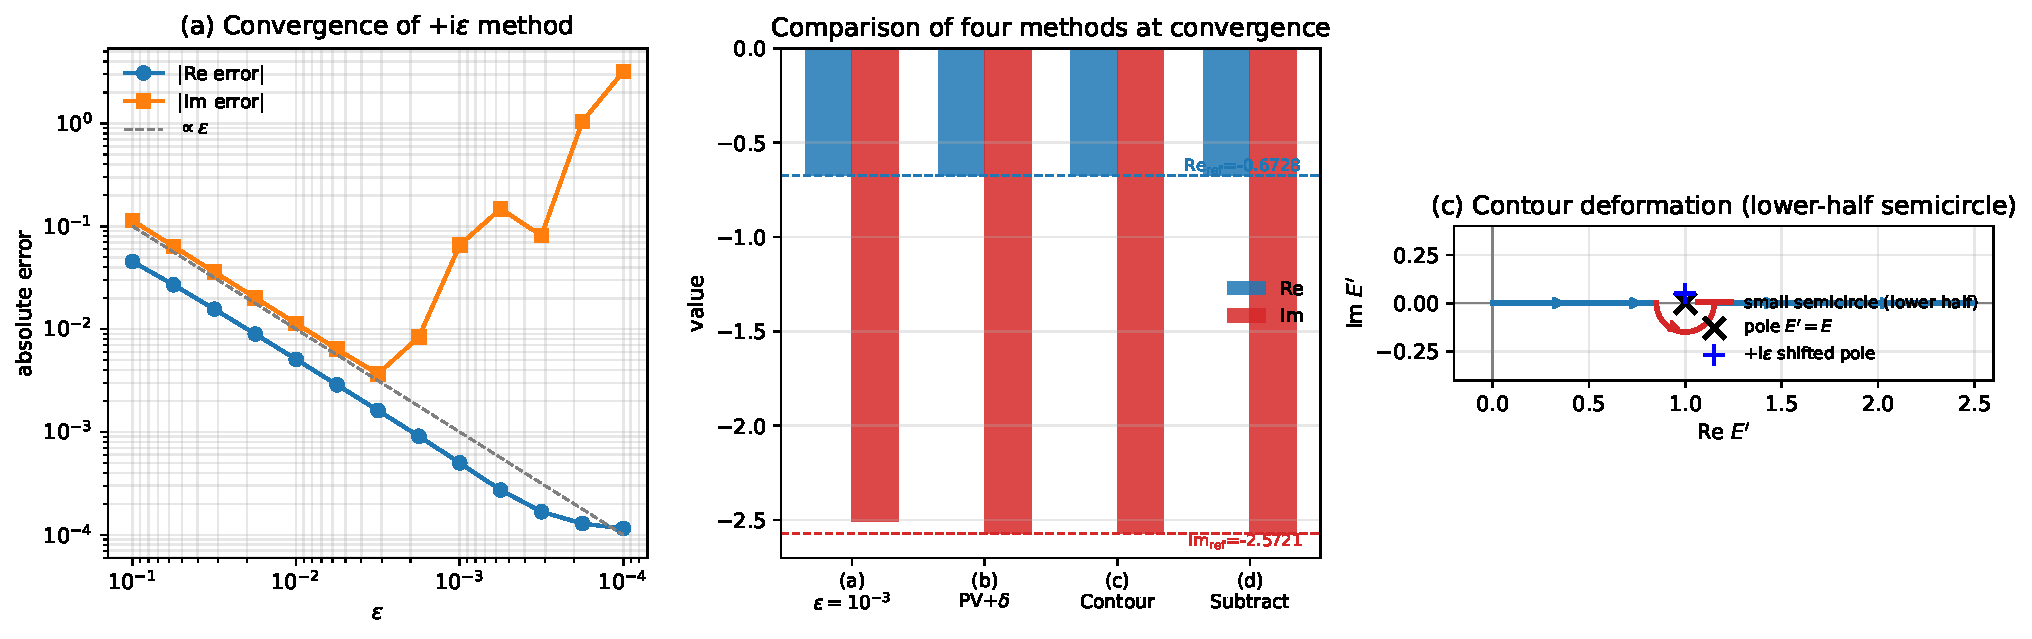
\includegraphics[width=0.98\linewidth]{ch07_pole_bypass}
    \caption{极点绕走的四种处理方式。
    左：方法 (a) 的绝对误差关于 $\epsilon$ 的扫描，
    实部误差 $\propto\epsilon^2$ (Lorentzian 偏置经过对称积分相消后剩二阶)，
    虚部误差 $\propto\epsilon$ (Lorentzian 与 $\delta$ 的有限宽度差异).
    中：四种方法在 \emph{已收敛} 取值下的实部 / 虚部柱状对比，
    虚线为参考解 $\Re I=-0.6728$, $\Im I=-\pi f(E)\approx -2.5721$。
    方法 (b)(c)(d) 与参考值的差异已在 $10^{-7}$ 量级内 (求积本身的离散误差)。
    右：方法 (c) 在复 $E'$-平面上的围道示意。
    极点 $E'=E$ 落在围道之外 (蓝色 $+\rmi\epsilon$ 移位极点亦如此)，
    下半圆贡献 $-\rmi\pi f(E)$ 即 \eqref{eq:numexp-ch07-SP} 中的 $\delta$ 部分。}
    \label{fig:numexp-ch07}
\end{figure}

数值结果 (脚本输出)：
\begin{center}\small
\begin{tabular}{lcc}
\hline
方法 & $\Re I$ & $\Im I$ \\
\hline
参考解 (高精度自适应)             & $-0.67280067$ & $-2.57211852$ \\
(a) $+\rmi\epsilon$, $\epsilon=10^{-3}$ & $-0.67330$    & $-2.50637$    \\
(b) PV $+\delta$ 拆分              & $-0.67280067$ & $-2.57211852$ \\
(c) 围道形变 ($r=10^{-3}$)        & $-0.67280067$ & $-2.57211852$ \\
(d) 减法 $+$ 解析修正              & $-0.67280067$ & $-2.57211852$ \\
\hline
\end{tabular}
\end{center}

\subsection*{物理讨论}

\begin{itemize}
  \item \textbf{(a) 的本质是磨平 (regularization).}
        把 $\delta$-函数换成宽度 $\epsilon$ 的 Lorentzian
        $\frac{1}{\pi}\frac{\epsilon}{(E-E')^2+\epsilon^2}$；要逼近 $\delta$ 必须 $\epsilon\to 0$，
        但同时积分网格也必须比 $\epsilon$ 更细才能分辨 Lorentzian 峰，
        因此实践上需要 $\epsilon\,\Delta E^{-1}\gtrsim 10$，
        而 $\Im$ 误差仍只能以 $\epsilon$ 一阶下降。
        $+\rmi\epsilon$ 在\emph{形式推导} 中无可替代，
        但若直接用作数值方案则收敛缓慢。
  \item \textbf{(b) 是教科书做法。}
        把奇异性\emph{解析地} 处理掉之后，
        余下的被积函数完全光滑，求积可以达到机器精度。
        代价是要求被积权重 $f(E')$ 在极点处可微 (取 $f(E')-f(E)$)。
  \item \textbf{(c) 给出 $+\rmi\epsilon$ 处方的几何意义。}
        $+\rmi\epsilon$ 把极点抬到上半平面等价于把围道压到下半平面。
        在与时间有关的描述中 (cf.\ 第 \ref{ch:Smat1P}, \ref{ch:cross} 章)，
        $+\rmi 0^+$ 选取的正是\emph{出射} ($t\to+\infty$) 边界条件：
        极点的小虚部对应于\emph{衰减的入射波尾}, $\rme^{-\epsilon t}$，
        把因果性翻译成围道方向的具体规则。
        这是 $G^+$ vs $G^-$ 二分法在数值层面的几何呈现。
  \item \textbf{(d) 是色散关系的"主力".}
        在第 \ref{ch:analytic} 章我们要从 $\Im T(E)$ 的实验测量
        重构 $\Re T(E)$ (Kramers--Kronig / forward dispersion)：
        实部恰好是 \eqref{eq:numexp-ch07-main} 的形式。
        减法做得更进一步、可以取多次减除以保证大 $E'$ 收敛，
        是高能物理 / 核物理 / 光学色散分析的标准操作。
\end{itemize}

四种方法对同一物理量给出一致的数值，
彼此互相充当交叉验证；
\eqref{eq:Gpm-def} 中的 $\pm\rmi 0^+$ 不再是符号上的"小修饰"，
而是\emph{有具体可计算后果} 的物理边界条件。

\chapter{Born 级数与 Lippmann--Schwinger 方程 (Born Series)}\label{ch:born}

前一章我们引入了 Green 算符 $G_0(z)=(z-\Hmat_0)^{-1}$ 与全空间 Green 算符 $G(z)=(z-\Hmat)^{-1}$，并得到 Lippmann--Schwinger 方程
\begin{equation}
\Tmat(z)=\Vmat+\Vmat\,G_0(z)\,\Tmat(z),\qquad
G(z)=G_0(z)+G_0(z)\,\Vmat\,G(z).
\label{eq:LS-recall}
\end{equation}
在能壳上 (on-shell) 取 $z=E_p+\rmi 0$, 即可得到 $T$ 矩阵元
\begin{equation}
t(\bm p'\!\leftarrow\bm p)=\matel{\bm p'}{\Tmat(E_p+\rmi 0)}{\bm p},
\end{equation}
它直接给出散射振幅 $f(\bm p'\!\leftarrow\bm p)=-(2\pi)^2 m\,t(\bm p'\!\leftarrow\bm p)$ 与微分截面。本章的目标是构造 \eqref{eq:LS-recall} 的迭代解 (Born 级数), 讨论其收敛性、最低阶 (玻恩) 近似的物理图像与适用范围, 并通过 Yukawa 势、电子-原子散射等例子加以说明。最后我们指出 Born 级数也可以视为相互作用图像下 $S$ 算符的微扰展开, 给出对应的 Feynman 图规则。

\section{Born 级数的形式构造}\label{sec:born-formal}

\subsection{从 Lippmann--Schwinger 方程出发的迭代}

为了引入合适的小参数, 把相互作用部分写成 $\Vmat\to\lambda\Vmat$, 把 $\lambda$ 看作从 $V$ 中抽出的耦合常数, 最后取 $\lambda\to 1$. 哈密顿量为
\begin{equation}
\Hmat=\Hmat_0+\lambda\Vmat.
\end{equation}
对应的 Lippmann--Schwinger 方程
\begin{equation}
\Tmat(z)=\lambda\Vmat+\lambda\Vmat\,G_0(z)\,\Tmat(z)
\label{eq:LS-lambda}
\end{equation}
是 $\Tmat$ 的算符方程。形式上把它解出来得
\begin{equation}
\bigl[1-\lambda\Vmat\,G_0(z)\bigr]\Tmat(z)=\lambda\Vmat
\;\Longrightarrow\;
\Tmat(z)=\bigl[1-\lambda\Vmat\,G_0(z)\bigr]^{-1}\lambda\Vmat
=\sum_{n=0}^{\infty}\bigl(\lambda\Vmat\,G_0(z)\bigr)^{n}\lambda\Vmat.
\label{eq:born-T}
\end{equation}
若把 $\Tmat(z)$ 关于 $\lambda$ 做形式幂级数展开
\begin{equation}
\Tmat(z)=\sum_{n=0}^{\infty}\lambda^{n}\Tmat^{(n)}(z),
\end{equation}
比较 \eqref{eq:LS-lambda} 两边各阶的系数可得
\begin{equation}
\Tmat^{(0)}=0,\quad \Tmat^{(1)}=\Vmat,\quad
\Tmat^{(n)}=\Vmat\bigl(G_0\Vmat\bigr)^{n-1}=\bigl(\Vmat G_0\bigr)^{n-1}\Vmat,\;n\ge 1.
\end{equation}
取 $\lambda\to 1$ 给出 \emph{Born 级数}
\begin{equation}
\boxed{\;\Tmat(z)=\Vmat+\Vmat G_0(z)\Vmat+\Vmat G_0(z)\Vmat G_0(z)\Vmat+\cdots
=\sum_{n=0}^{\infty}\Vmat\bigl(G_0(z)\Vmat\bigr)^{n}\;}
\label{eq:born-series}
\end{equation}
对应于波函数与 Green 算符的级数为
\begin{align}
\ket{\psi^{\pm}}&=\ket{\phi}+G_0^{\pm}\Vmat\ket{\phi}+G_0^{\pm}\Vmat G_0^{\pm}\Vmat\ket{\phi}+\cdots,\\
G(z)&=G_0(z)+G_0(z)\Vmat G_0(z)+G_0(z)\Vmat G_0(z)\Vmat G_0(z)+\cdots .
\end{align}

\subsection{On-shell $T$ 矩阵元的展开}

把 \eqref{eq:born-T} 投影到自由动量本征态 $\ket{\bm p}$, 并取 $z=E_p+\rmi 0$:
\begin{equation}
t(\bm p'\!\leftarrow\bm p)
=\lambda\matel{\bm p'}{V}{\bm p}
+\lambda^{2}\matel{\bm p'}{V\,G_0(E_p+\rmi 0)\,V}{\bm p}+\cdots .
\label{eq:T-expansion}
\end{equation}
令 $\lambda\to 1$, 第 $n$ 项即 $t^{(n)}(\bm p'\!\leftarrow\bm p)$.

\begin{remark}[Born 级数的一般性质]
\begin{itemize}
  \item Born 级数不一定收敛。
  \item 即使收敛, 也不一定收敛得很快, 前几阶不一定给出主要贡献。
  \item 在某些情形下收敛得足够快, 特别是高能或者势足够弱时, 最低阶的几项可能就给出主要贡献。
  \item 即便仅知道收敛性, Born 级数也可以用来在理论上推出散射振幅的一些一般性质 (例如解析性、幺正性等)。
  \item 当确实没有别的方法时, Born 近似往往是唯一可用的工具。
\end{itemize}
\end{remark}

\section{收敛性条件}\label{sec:convergence}

我们期望当算符 $\lambda\Vmat\,G_0$ 在某种范数下足够 “小” 时, \eqref{eq:born-T} 中的几何级数收敛。直观上, 有两种使其变小的途径:
\begin{enumerate}
  \item $\lambda$ 充分小, 即耦合常数足够弱;
  \item 能量 $E_p$ 充分大, 此时 $G_0=(z-\Hmat_0)^{-1}$ 在算符范数意义下变小。
\end{enumerate}
在适当条件下 (例如 $V$ 满足前章中保证 $T$ 矩阵存在的条件), 可以严格证明下列两条结论。

\begin{theorem}[弱耦合下的收敛性]\label{thm:weak-coupling}
对于任何势 $V$, 存在 $\bar\lambda>0$ 使得对所有 $|\lambda|<\bar\lambda$ 与所有 $\bm p,\bm p'$, Born 级数 \eqref{eq:T-expansion} 收敛到正确的 on-shell $T$ 矩阵元. $\lambda$ 越小, 收敛越快, 第一项 (Born 近似) 给出主要贡献。
\end{theorem}

\begin{theorem}[高能区的收敛性]\label{thm:high-energy}
对任何势 $V$, 存在 $\bar E$ 使得当 $E>\bar E$ 时, Born 级数在 $\lambda=1$ 时都收敛. $E$ 越大, 收敛越快; 对足够大的 $E$, 第一项 Born 近似给出主要贡献。
\end{theorem}

\begin{remark}[束缚态与收敛性的关系]
若 $\lambda$ 足够小使得 Born 级数对所有 $E>0$ 都收敛, 那么 $\lambda V$ 没有束缚态 (Green 算符 $G(z)$ 在 $z=E_p+\rmi 0$ 附近正则). 反过来, 如果势 $V$ 支持束缚态, 那么相应的 Born 级数无法对所有正能量都收敛 —— 因为某些 $E>0$ 邻域内 $G$ 的解析延拓附近会出现极点或不规则性的痕迹, 而 \eqref{eq:born-T} 中的几何级数无法描述这种结构。
\end{remark}

\section{第一阶 Born 近似}\label{sec:first-born}

\subsection{$T$ 矩阵元与散射振幅}

仅保留 \eqref{eq:T-expansion} 的第一项就得到 \emph{Born 近似 (first Born approximation)}:
\begin{equation}
t^{(1)}(\bm p'\!\leftarrow\bm p)=\matel{\bm p'}{V}{\bm p}.
\label{eq:T1}
\end{equation}
利用平面波归一化 $\inn{\bm x}{\bm p}=(2\pi)^{-3/2}\rme^{\rmi\bm p\cdot\bm x}$, 散射振幅为
\begin{align}
f^{(1)}(\bm p'\!\leftarrow\bm p)
&=-(2\pi)^{2}m\,\matel{\bm p'}{V}{\bm p}\notag\\
&=-\frac{m}{2\pi}\int\rmd^{3}x\;\rme^{-\rmi\bm p'\cdot\bm x}\,V(\bm x)\,\rme^{\rmi\bm p\cdot\bm x}\notag\\
&=-\frac{m}{2\pi}\int\rmd^{3}x\;\rme^{-\rmi\bm q\cdot\bm x}\,V(\bm x),
\quad \bm q\equiv\bm p'-\bm p.
\label{eq:f1-Fourier}
\end{align}
即 \emph{第一阶 Born 振幅是相互作用势的 Fourier 变换}, 仅依赖于动量转移 (momentum transfer)
\begin{equation}
\bm q=\bm p'-\bm p,\qquad q\equiv|\bm q|=2p\sin\frac{\theta}{2},
\end{equation}
其中 $\theta$ 是散射角, 弹性碰撞下 $|\bm p'|=|\bm p|=p$.

\begin{remark}
由 \eqref{eq:f1-Fourier} 的对称形式可以直接读出 Born 近似的两个一般特征:
\begin{enumerate}
  \item $f^{(1)}(\bm p'\!\leftarrow\bm p)=f^{(1)}(\bm p\!\leftarrow\bm p')^{*}$ 当 $V$ 实时, 而对实势 $V(\bm x)\in\R$, $f^{(1)}$ 还是 $\bm q$ 的实函数 (经 Fourier 变换后实势的 Fourier 变换是实函数, 当且仅当 $V(\bm x)=V(-\bm x)$)。
  \item 仅依赖 $|\bm q|$ (球对称势的情况下), 入射方向自动转移到末态。
\end{enumerate}
\end{remark}

\subsection{球对称势}

若 $V(\bm x)=V(r)$, 对 $\bm x$ 角度积分得
\begin{equation}
f^{(1)}(\bm p'\!\leftarrow\bm p)=-2m\int_{0}^{\infty}\rmd r\;r^{2}\,\frac{\sin qr}{qr}\,V(r).
\label{eq:f1-spherical}
\end{equation}

\begin{remark}[Born 近似的若干性质]
\begin{itemize}
  \item \textbf{向前散射振幅}. 当 $\bm p'=\bm p$ 时 $\bm q=0$, 由 \eqref{eq:f1-spherical}
\begin{equation}
f^{(1)}(\bm p\!\leftarrow\bm p)=-2m\int_{0}^{\infty}\rmd r\;r^{2}V(r),
\end{equation}
为常数, 与能量无关。
  \item \textbf{零能极限}. $q=0$ 时 $f^{(1)}(\bm p\!\leftarrow\bm p)$ 仍是上式, 对所有方向都相同。
  \item \textbf{向前峰}. 当 $q$ 变大时 $f^{(1)}\to 0$, 由 $q=2p\sin(\theta/2)$, 这意味着 $\theta$ 增大或能量增大 (入射动量 $p$ 增大) 时振幅减小. 能量越高, 振幅随角度的下降越快, 形成显著的向前峰。
  \item \textbf{幺正性}. 向前散射振幅在 Born 近似下是实数, 而光学定理要求 $\mathrm{Im}\,f(\bm p\!\leftarrow\bm p)=\dfrac{p}{4\pi}\int\rmd\Omega\,|f|^{2}\ge 0$, 故 Born 近似 \emph{违反} 幺正性。注意 $f^{(1)}\sim O(\lambda)$, 但 $|f|^{2}\sim O(\lambda^{2})$, 仅算到 $O(\lambda)$ 是无虚部的, 所以这种违反在弱耦合下数值很小, 必须算到 $f^{(2)}$ 才能看到光学定理两边一致。
\end{itemize}
\end{remark}

\subsection{Born 级数与幺正性}

由 $\Smat=1-2\pi\rmi\,\delta(E_{p'}-E_{p})\,\Tmat$, 把 $\Smat$ 展开为
\begin{equation}
\Smat=1+\lambda \Smat^{(1)}+\lambda^{2}\Smat^{(2)}+\cdots ,
\end{equation}
代入幺正性条件 $\Smat^{\dagger}\Smat=1$:
\begin{equation}
1+\lambda\bigl[\Smat^{(1)}+\Smat^{(1)\dagger}\bigr]
+\lambda^{2}\bigl[\Smat^{(1)\dagger}\Smat^{(1)}+\Smat^{(2)}+\Smat^{(2)\dagger}\bigr]+\cdots=1.
\end{equation}
逐阶比较系数:
\begin{align}
\Smat^{(1)}+\Smat^{(1)\dagger}&=0,\label{eq:S-unit-1}\\
\Smat^{(1)\dagger}\Smat^{(1)}+\Smat^{(2)}+\Smat^{(2)\dagger}&=0,\label{eq:S-unit-2}\\
&\;\;\vdots\notag
\end{align}
\eqref{eq:S-unit-1} 给出 $f^{(1)}(\bm p'\!\leftarrow\bm p)^{*}=f^{(1)}(\bm p\!\leftarrow\bm p')$, 故 \emph{幺正性已经决定向前散射的 Born 近似必为实数}. 若不算到 $\Smat^{(2)}$, 则 \eqref{eq:S-unit-2} 不成立; 但若 Born 级数收敛足够快, $\Smat^{(2)}$ 可以忽略不计, 则违反幺正性的程度比较小。如果 Born 级数收敛得不够快, 幺正性则会被严重破坏。

\section{第二阶 Born 近似}\label{sec:second-born}

为了估计 Born 近似的好坏, 我们计算 Born 级数的第二项. 由 \eqref{eq:T-expansion}
\begin{align}
f^{(2)}(\bm p'\!\leftarrow\bm p)
&=-(2\pi)^{2}m\,\matel{\bm p'}{V\,G_0(E_p+\rmi 0)\,V}{\bm p}\notag\\
&=-(2\pi)^{2}m\int\rmd^{3}p''\;\frac{\matel{\bm p'}{V}{\bm p''}\,\matel{\bm p''}{V}{\bm p}}{E_{p}-E_{p''}+\rmi 0}.
\label{eq:f2-general}
\end{align}
中间态 $\bm p''$ 是 \emph{所有} 自由中间态 (包括能量壳之外) 的积分, $G_0$ 中 $+\rmi 0$ 处方使得能壳上 ($E_{p''}=E_p$) 的奇异性按出射边界条件解释。

\section{例：Yukawa 势}\label{sec:yukawa}

\subsection{第一阶振幅与微分截面}

Yukawa 势最初由汤川 (Yukawa) 在介子理论中提出, 用以描述核子-核子之间通过交换有质量介子产生的相互作用; 在原子物理中也可用作屏蔽 Coulomb 势的近似:
\begin{equation}
V(r)=\gamma\,\frac{\rme^{-\mu r}}{r}.
\end{equation}
代入 \eqref{eq:f1-spherical} 直接积分得
\begin{equation}
f^{(1)}(\bm p'\!\leftarrow\bm p)=-\frac{2\gamma m}{\mu^{2}+q^{2}},\qquad q=2p\sin\frac{\theta}{2}.
\label{eq:f1-yukawa}
\end{equation}
此振幅与 “交换一个标量场粒子" 的振幅同形, $\mu$ 即介子质量. 若取 $\pi$ 介子参数 $\mu\sim 140\,\mathrm{MeV}/c^{2}$, $\gamma\sim -2c/3$, 可大致描述核子的长程相互作用 (single-pion exchange). 微分散射截面 (质心系下) 为
\begin{equation}
\frac{\rmd\sigma}{\rmd\Omega}=|f^{(1)}|^{2}
=\frac{4\gamma^{2}m^{2}}{\bigl(\mu^{2}+4p^{2}\sin^{2}\frac{\theta}{2}\bigr)^{2}}.
\label{eq:dsigma-yukawa}
\end{equation}
当 $p\gg\mu$ 时, 向前峰的角宽度 $\sim\mu/p$.

\begin{remark}[屏蔽 Coulomb 极限]
取 $\mu\to 0$ 给出 Coulomb 散射: $f^{(1)}\to-2\gamma m/q^{2}=-\gamma m/(2p^{2}\sin^{2}(\theta/2))$. 由此立得 Rutherford 公式
\begin{equation}
\frac{\rmd\sigma}{\rmd\Omega}\xrightarrow[\mu\to 0]{}
\frac{\gamma^{2}m^{2}}{4p^{4}\sin^{4}(\theta/2)} ,
\end{equation}
这是 Born 近似与精确 Coulomb 结果的一致点 (尽管纯 Coulomb 势不满足前述短程性条件, Born 级数其余各阶发散; 但屏蔽提供天然正则化, $\mu\to 0$ 极限对截面公式是良好的).
\end{remark}

\subsection{第二阶振幅与玻恩近似可靠性}

代入 Yukawa 势后, 经过角积分与三维主值积分, \eqref{eq:f2-general} 在向前散射 ($\bm p'=\bm p$) 给出
\begin{equation}
f^{(2)}(\bm p\!\leftarrow\bm p)
=\frac{2\gamma^{2}m^{2}}{\mu^{2}(\mu-2\rmi p)}.
\label{eq:f2-yukawa-fwd}
\end{equation}
要求 Born 近似可靠等价于 $|f^{(2)}|\ll|f^{(1)}|$. 把 $\theta=0$ 的两个表达式作比有
\begin{equation}
\left|\frac{f^{(2)}}{f^{(1)}}\right|=\frac{\gamma m}{(\mu^{2}+4p^{2})^{1/2}},\qquad \theta=0.
\label{eq:ratio-yukawa}
\end{equation}

\begin{itemize}
  \item 对 \emph{核子-核子} 情形, $\gamma\sim -2c/3$, $m\sim 500\,\mathrm{MeV}/c^{2}$, $\mu\sim 140\,\mathrm{MeV}/c$, 在 $p=0$ 时 $|f^{(2)}/f^{(1)}|\sim 2.5$, Born 近似显然不成立。
  \item 当能量升高 $p^{2}\gg\mu^{2}$ 时, 核子运动应是相对论性的, 此时非相对论近似本身不再可靠。
  \item $\theta\ne 0$ 时需要计算 \eqref{eq:f2-general} 一般情形的 $f^{(2)}(\bm p'\!\leftarrow\bm p)$, 方法类似但代数较繁。
\end{itemize}

\noindent 最终结论是: 对 Yukawa 势
\begin{equation}
\text{(low energy, } p<\mu\text{)}: \;\Bigl|\frac{\gamma m}{\mu}\Bigr|\ll 1;\qquad
\text{(high energy, } p>\mu\text{)}: \;\Bigl|\frac{\gamma m}{p}\Bigr|\ll 1.
\end{equation}
直接应用 Born 近似讨论核子-核子散射不是一个好的近似; 但在分波振幅或较高能区, Born 级数仍可能给出有用的指导.

\section{例：电子-原子散射}\label{sec:e-atom}

\subsection{静态近似与 Born 近似的双重近似}

弹性散射近似下, 把原子看成是固定的电荷分布 $\rho(\bm x)$, 称为 \emph{静态近似} (``static" approximation 或 ``one-state" approximation). 电子看到的势为
\begin{equation}
V(\bm x)=-e\int\rmd^{3}x'\;\frac{\rho(\bm x')}{|\bm x-\bm x'|}.
\end{equation}
这是 Poisson 方程的经典解, 对应于忽略原子内部激发的 elastic-only 通道。

\subsection{电子-氢原子散射}

考虑电子与氢原子的散射, 中心为质子 $\delta(\bm x)$ 加上束缚电子电荷密度 $-e|\phi(\bm x)|^{2}$ (基态波函数 $\phi(\bm x)=(\pi a^{3})^{-1/2}\rme^{-r/a}$, $a$ 为 Bohr 半径). 总电荷密度
\begin{equation}
\rho(\bm x)=e\Bigl\{\delta_{3}(\bm x)-|\phi(\bm x)|^{2}\Bigr\}.
\end{equation}
对应的球对称势 (经过卷积积分后)
\begin{equation}
V(r)=-e^{2}\Bigl(\frac{1}{r}+\frac{1}{a}\Bigr)\rme^{-2r/a}.
\end{equation}
代入 \eqref{eq:f1-spherical} 得
\begin{equation}
f^{(1)}(\bm p'\!\leftarrow\bm p)
=-2m\int_{0}^{\infty}\rmd r\,r^{2}\,\frac{\sin qr}{qr}\,V(r)
=2 a\,\frac{8+q^{2}a^{2}}{(4+q^{2}a^{2})^{2}}.
\label{eq:f1-eH}
\end{equation}
本结果实际涉及两层近似: (1) 静态近似 $V(\bm x)$; (2) 玻恩近似. 两者可分别讨论。

\paragraph{Born 近似的可靠性.}
为定性估计, 用 Yukawa 势近似氢原子势, 取 $\gamma=-e^{2}$, $\mu\sim 1/a$, 在 0 与 $\infty$ 附近渐近行为接近. 沿用 \eqref{eq:ratio-yukawa}:
\begin{itemize}
\item $p\ll\mu\sim 1/a$ 时, $\bigl|\dfrac{\gamma m}{\mu}\bigr|\sim e^{2}ma\ll 1$, 但 $a=1/(me^{2})$, $e^{2}ma=1$, \emph{不满足}, 故低能时 Born 近似失败 (这与精确分波分析一致, 低能 $S$ 波散射长度对应原子的极化与束缚态情况).
\item $p\gg\mu\sim 1/a$, 要求 $\bigl|\dfrac{\gamma m}{p}\bigr|\sim\dfrac{e^{2}m}{p}\ll 1$, 即 $pa\gg 1$. 入射波长必须远小于 Bohr 半径, 等价于入射电子动能远大于约 $10\,\mathrm{eV}$. 因此, 对入射能量 $\gtrsim 100\,\mathrm{eV}$ 时 Born 近似才开始可信。
\end{itemize}

\subsection{电子-氦原子散射}

由于氢原子并不以原子形式自然存在, 实验上更常用 He 等惰性气体. 静态近似下, 电荷分布
\begin{equation}
\rho(\bm x)=e\Bigl\{2\delta_{3}(\bm x)-\int\rmd^{3}x_{2}|\phi(\bm x,\bm x_{2})|^{2}-\int\rmd^{3}x_{1}|\phi(\bm x_{1},\bm x)|^{2}\Bigr\}.
\end{equation}
$\phi(\bm x_{1},\bm x_{2})$ 为基态两电子波函数, 没有严格解析解. 常用的近似形式为
\begin{equation}
\phi(\bm x_{1},\bm x_{2})=\chi(\bm x_{1})\chi(\bm x_{2}),\quad
\chi(\bm x)=\alpha(\pi a^{3})^{-1/2}\rme^{-zr/a}+\beta(\pi a^{3})^{-1/2}\rme^{-2zr/a}/\,\sqrt{8},
\end{equation}
最佳变分估计为 $\alpha=1.48,\beta=-0.61,z=1.45$. 由 $\rho(\bm x)$ 求 $V(\bm x)$, 再由 $V(\bm x)$ 在 Born 近似下得到
\begin{equation}
\begin{aligned}
&f^{(1)}(\bm p'\!\leftarrow\bm p)\\
&\quad=\frac{\alpha^{2}}{z^{3}}a\Biggl[
4\,\frac{8z^{2}+q^{2}a^{2}}{(4z^{2}+q^{2}a^{2})^{2}}
+\frac{64\beta}{27}\,\frac{18z^{2}+q^{2}a^{2}}{(9z^{2}+q^{2}a^{2})^{2}}
+\frac{\beta^{2}}{2}\,\frac{32z^{2}+q^{2}a^{2}}{(16z^{2}+q^{2}a^{2})^{2}}
\Biggr].
\end{aligned}
\end{equation}
类似于电子-氢原子散射, 估算可知电子能量高于约 $100\,\mathrm{eV}$ 时 Born 近似比较可信. 在 $500\,\mathrm{eV}$ 时 Born 近似的微分截面与实验 (Hughes \emph{et al.}, Heutzberg) 数据除向前散射附近外吻合较好。

\section{Born 级数与 $S$ 矩阵的微扰展开}\label{sec:S-perturbation}

Born 级数也可以等价地从相互作用图像下 $S$ 算符的微扰展开导出, 这种构造给出每一阶项的直观时空图像与 Feynman 图规则。

\subsection{Schrödinger 与相互作用图像}

\paragraph{Schrödinger 图像.}
算符 $\Op X,\Op P,\Smat,\ldots$ 不随时间演化, 态满足
\begin{equation}
\ket{\psi(t)}_{S}=\rme^{-\rmi\Hmat(t-t_{0})}\ket{\psi(t_{0})}_{S}.
\end{equation}

\paragraph{相互作用 (Dirac) 图像.}
\begin{equation}
\ket{\psi(t)}_{I}=\rme^{\rmi\Hmat_{0}t}\ket{\psi(t)}_{S},\quad
\Op A_{I}(t)=\rme^{\rmi\Hmat_{0}t}\Op A_{S}\,\rme^{-\rmi\Hmat_{0}t}.
\end{equation}
两图像下可观测量 (矩阵元) 相同:
${}_{I}\matel{\phi}{\Op A_{I}}{\psi}_{I}={}_{S}\matel{\phi}{\Op A_{S}}{\psi}_{S}$. 关键观察是: 若 $\ket{\psi}_{S}$ 是散射态, 则 $\ket{\psi(t\to\mp\infty)}_{I}$ 在 Schrödinger 图像下的渐近态 $\ket{\psi_{\mathrm{in/out}}}_{S}$. 因此相互作用图像下散射对应于
$t\to -\infty$ 渐近态 $\ket{\psi_{\mathrm{in}}}_{S}\;\to\; t\to +\infty$ 渐近态 $\ket{\psi_{\mathrm{out}}}_{S}$.

\subsection{$S$ 算符的 Dyson 展开}

Schrödinger 图像演化算符 $U_{S}(t,t_{0})=\rme^{-\rmi\Hmat(t-t_{0})}$, 相互作用图像演化算符
\begin{equation}
U_{I}(t,t_{0})=\rme^{\rmi\Hmat_{0}t}\rme^{-\rmi\Hmat(t-t_{0})}\rme^{-\rmi\Hmat_{0}t_{0}}.
\end{equation}
$S$ 算符即两个无穷远的渐近极限 (实际为弱极限)
\begin{equation}
\Smat=\lim_{\substack{t\to+\infty\\ t_{0}\to-\infty}}
\rme^{\rmi\Hmat_{0}t}\rme^{-\rmi\Hmat(t-t_{0})}\rme^{-\rmi\Hmat_{0}t_{0}}=U_{I}(\infty,-\infty).
\label{eq:S-UI}
\end{equation}
$U_{I}$ 满足
\begin{equation}
\rmi\partial_{t}U_{I}(t,t_{0})=V_{I}(t)\,U_{I}(t,t_{0}),\qquad
V_{I}(t)\equiv \rme^{\rmi\Hmat_{0}t}\Vmat\,\rme^{-\rmi\Hmat_{0}t}.
\end{equation}
积分形式为 $U_{I}(t,t_{0})=1-\rmi\int_{t_{0}}^{t}\rmd\tau\,V_{I}(\tau)\,U_{I}(\tau,t_{0})$, 迭代得 \emph{Dyson 级数}:
\begin{equation}
U_{I}(t,t_{0})=1-\rmi\int_{t_{0}}^{t}\rmd\tau\,V_{I}(\tau)
+(-\rmi)^{2}\int_{t_{0}}^{t}\rmd\tau'\int_{t_{0}}^{\tau'}\rmd\tau\,V_{I}(\tau')V_{I}(\tau)+\cdots .
\label{eq:dyson}
\end{equation}

\subsection{$S$ 矩阵元的微扰展开}

取 $t\to\infty,t_{0}\to-\infty$, 在动量本征态间取矩阵元:
\begin{align}
\matel{\bm p'}{\Smat}{\bm p}
&=\delta_{3}(\bm p'-\bm p)
-\rmi\int_{-\infty}^{\infty}\rmd\tau\;\rme^{\rmi E_{p'}\tau}\matel{\bm p'}{V}{\bm p}\,\rme^{-\rmi E_{p}\tau}\notag\\
&\quad+(-\rmi)^{2}\int_{-\infty}^{\infty}\rmd\tau'\int_{-\infty}^{\tau'}\rmd\tau\;
\rme^{\rmi E_{p'}\tau'}\matel{\bm p'}{V\,\rme^{-\rmi\Hmat_{0}(\tau'-\tau)}\,V}{\bm p}\,\rme^{-\rmi E_{p}\tau}+\cdots\notag\\
&\equiv \delta_{3}(\bm p'-\bm p)+\matel{\bm p'}{\Smat^{(1)}}{\bm p}+\matel{\bm p'}{\Smat^{(2)}}{\bm p}+\cdots .
\label{eq:S-pert}
\end{align}
此式称为 $S$ 矩阵元的 \emph{微扰展开} (perturbation expansion).

\subsection{各阶物理图像}

\paragraph{第一阶 ($\Smat^{(1)}$).}
完成 $\tau$ 积分得
\begin{equation}
\matel{\bm p'}{\Smat^{(1)}}{\bm p}
=-\rmi\int_{-\infty}^{\infty}\rmd\tau\,\rme^{\rmi(E_{p'}-E_{p})\tau}\matel{\bm p'}{V}{\bm p}
=-2\pi\rmi\,\delta(E_{p'}-E_{p})\,\matel{\bm p'}{V}{\bm p}.
\end{equation}
与 $\Smat=1-2\pi\rmi\delta(E_{p'}-E_{p})\Tmat$ 比较, 立得
\begin{equation}
t^{(1)}(\bm p'\!\leftarrow\bm p)=\matel{\bm p'}{V}{\bm p},
\end{equation}
正是 \eqref{eq:T1}. 物理上: 入射态 $\ket{\bm p}$ 自由运动到时刻 $\tau$, 突然感受到 $V$ 的相互作用变成 $\ket{\bm p'}$, 然后再自由运动出去, 然后对所有可能的 $\tau$ 积分。

\paragraph{第二阶 ($\Smat^{(2)}$).}
\begin{equation}
\matel{\bm p'}{\Smat^{(2)}}{\bm p}
=(-\rmi)^{2}\int_{-\infty}^{\infty}\rmd\tau'\int_{-\infty}^{\tau'}\rmd\tau\int\rmd^{3}k\;
\rme^{\rmi(E_{p'}-E_{k})\tau'}\matel{\bm p'}{V}{\bm k}\matel{\bm k}{V}{\bm p}\rme^{-\rmi(E_{p}-E_{k})\tau}.
\end{equation}
内层 $\tau$ 积分 $\int_{-\infty}^{\tau'}\rmd\tau\,\rme^{-\rmi(E_{p}-E_{k})\tau}$ 在严格意义下不收敛, 必须考虑初末态是 (实验上必然如此的) 波包, 这样积分自动收敛. 等价地在指数中加入 $\rme^{-\epsilon|\tau|}$ 因子 ($\epsilon\to 0^{+}$):
\begin{equation}
\int_{-\infty}^{\tau'}\rmd\tau\,\rme^{-\rmi(E_{p}-E_{k}+\rmi\epsilon)\tau}
=\frac{\rmi\,\rme^{-\rmi(E_{p}-E_{k})\tau'}}{E_{p}-E_{k}+\rmi 0}.
\end{equation}
代回并完成 $\tau'$ 积分得
\begin{equation}
\matel{\bm p'}{\Smat^{(2)}}{\bm p}
=-2\pi\rmi\,\delta(E_{p'}-E_{p})\int\rmd^{3}k\;\frac{\matel{\bm p'}{V}{\bm k}\matel{\bm k}{V}{\bm p}}{E_{p}-E_{k}+\rmi 0}.
\end{equation}
这正是 $\Tmat^{(2)}=\Vmat\,G_{0}(E_{p}+\rmi 0)\,\Vmat$ 的矩阵元. 物理图像: 入射态 $\ket{\bm p}$ 自由运动到 $\tau$, 被 $V$ 散射一下变成中间态 $\ket{\bm k}$ ($\bm k$ 不在能壳上), 又自由运动到 $\tau'$, 再被 $V$ 散射一下成为末态 $\ket{\bm p'}$, 之后自由出射. 然后对所有 $\bm k$ 求积分以及对所有时间 $\tau<\tau'$ 积分. 第三阶以及更高阶以此类推.

\subsection{Feynman 图规则 (非相对论)}

由上述展开可读出非相对论 Born 级数的 Feynman 规则: 第 $n$ 阶的项
\begin{equation}
t^{(n)}(\bm p'\!\leftarrow\bm p)
=\int\rmd^{3}k_{1}\cdots\rmd^{3}k_{n-1}\;
\frac{\matel{\bm p'}{V}{\bm k_{n-1}}\cdots\matel{\bm k_{2}}{V}{\bm k_{1}}\matel{\bm k_{1}}{V}{\bm p}}
{(E_{p}-E_{k_{n-1}}+\rmi 0)\cdots(E_{p}-E_{k_{1}}+\rmi 0)}
\end{equation}
可以读图得到, 规则如下:
\begin{enumerate}
  \item 画出有 $n$ 个相互作用顶点的 Feynman 图; 用一条 ``粒子线" 从入射 $\bm p=\bm k_{0}$ 串到出射 $\bm p'=\bm k_{n}$, 每个顶点表示一次与外势 $V$ 的作用.
  \item 对每一个顶点写出一个因子 $\matel{\bm k_{r+1}}{V}{\bm k_{r}}$, 其中 $\bm k_{0}=\bm p,\bm k_{n}=\bm p'$.
  \item 对每一个中间态 $\bm k=\bm k_{1},\ldots,\bm k_{n-1}$, 写下一个因子 $\dfrac{1}{E_{p}-E_{k}+\rmi 0}$.
  \item 对所有中间动量 $\bm k_{1},\ldots,\bm k_{n-1}$ 积分.
\end{enumerate}
注意这是 \emph{非相对论} 的 Feynman 规则; 相对论场论中的规则在传播子结构、反粒子、对称因子等方面更复杂.

\section{适用范围与扩展：DWBA 与 eikonal}\label{sec:extensions}

Born 近似在低能强耦合下严重失效. 实践中往往把 $\Vmat=\Vmat_{0}+\Vmat_{1}$ 拆为可解的 ``畸变" 部分 $\Vmat_{0}$ 与小的剩余部分 $\Vmat_{1}$, 对剩余部分作 Born 展开, 得到 \emph{畸变波 Born 近似} (DWBA):
\begin{equation}
t_{\text{DWBA}}(\bm p'\!\leftarrow\bm p)=\matel{\psi^{(-)}_{0}(\bm p')}{\Vmat_{1}}{\psi^{(+)}_{0}(\bm p)},
\end{equation}
其中 $\ket{\psi^{(\pm)}_{0}}$ 是哈密顿 $\Hmat_{0}+\Vmat_{0}$ 下的入/出态. 这一形式在核反应、电子-原子激发跃迁、直接反应等领域是基本工具.

另一类小角高能近似是 \emph{eikonal 近似}: 当 $ka\gg 1$ ($a$ 为势的力程, $k$ 为入射波数) 且偏转角小时, 散射波函数可近似写为 $\psi^{(+)}(\bm x)\approx\rme^{\rmi\bm k\cdot\bm x}\,\rme^{-\rmi\int_{-\infty}^{z}V(\bm b,z')\rmd z'/v}$, 散射振幅
\begin{equation}
f_{\text{eik}}(\theta)\approx -\rmi k\int\rmd^{2}b\,\rme^{\rmi\bm q\cdot\bm b}
\Bigl(\rme^{\rmi\chi(\bm b)}-1\Bigr),\quad
\chi(\bm b)=-\frac{1}{v}\int_{-\infty}^{\infty}V(\bm b,z)\rmd z.
\end{equation}
低阶展开 $\rme^{\rmi\chi}-1\approx\rmi\chi$ 即恢复高能 Born 近似, 而保留全部 $\chi$ 阶则相当于对 Born 级数做了无穷阶部分求和, 因而能正确描述高能小角下的多重散射相位累积。

\section*{本章小结}\addcontentsline{toc}{section}{本章小结}

\begin{itemize}
  \item Lippmann--Schwinger 方程 $\Tmat=\Vmat+\Vmat G_{0}\Tmat$ 形式上可解为几何级数 $\Tmat=\sum_{n}(\Vmat G_{0})^{n}\Vmat$, 即 \emph{Born 级数}.
  \item Born 级数收敛要求 $\Vmat G_{0}$ 在合适意义下小: 弱耦合 ($\lambda$ 小) 或高能 ($E$ 大) 时收敛, 收敛与束缚态的存在性互斥.
  \item 第一阶 Born 近似 $f^{(1)}(\bm q)=-\dfrac{m}{2\pi}\tilde V(\bm q)$ 表明散射振幅是势的 Fourier 变换; 仅依赖动量转移, 在 $\bm q=0$ 处与能量无关, 高能时形成向前峰.
  \item Born 近似破坏幺正性 (向前振幅为实, 违反光学定理), 但破坏程度由 Born 级数收敛速度控制.
  \item Yukawa 势 \eqref{eq:f1-yukawa}: 介子交换的标准模型范式; 核子-核子散射在低能下 Born 近似失败, 高能区受限于相对论效应.
  \item 电子-原子散射: 静态近似 + Born 近似. 电子能量 $\gtrsim 100\,\mathrm{eV}$ 时 Born 近似可信, 与实验吻合较好.
  \item Born 级数等价于 $S$ 算符在相互作用图像下的 Dyson 展开, 每一阶都有清晰的时空图像并对应一个非相对论 Feynman 图.
  \item 在 Born 近似不适用时, DWBA 与 eikonal 近似是最常用的两类拓展.
\end{itemize}

\section{本章定理证明补全}\label{sec:born-proofs}

本节集中给出第~\ref{sec:convergence} 节中两个收敛定理的证明骨架, 并补全
Born 级数与束缚态的关系, 以及 DWBA 的算符推导. 这些内容在第~\ref{ch:green}
章 (Green 算符) 与第~\ref{ch:stationary} 章 (定态散射) 中给出的算符基础上,
属于本章的核心技术.

\subsection{Neumann 级数收敛性 (算符范数)}

\begin{lemma}[几何级数引理]\label{lem:neumann}
设 $\Op K$ 是 Banach 空间 $\mathcal H$ 上的有界线性算符, 且
$\|\Op K\|<1$. 则 $1-\Op K$ 可逆且
\begin{equation}
(1-\Op K)^{-1}=\sum_{n=0}^{\infty}\Op K^{n},
\label{eq:born-neumann}
\end{equation}
级数在算符范数下绝对收敛, 且 $\|(1-\Op K)^{-1}\|\le (1-\|\Op K\|)^{-1}$.
\end{lemma}

\begin{proof}[证明]
部分和 $S_{N}=\sum_{n=0}^{N}\Op K^{n}$ 是 Cauchy 序列, 因为对 $M>N$
\begin{equation}
\|S_{M}-S_{N}\|\le\sum_{n=N+1}^{M}\|\Op K\|^{n}\le\frac{\|\Op K\|^{N+1}}{1-\|\Op K\|}\to 0.
\label{eq:born-neumann-cauchy}
\end{equation}
$\mathcal B(\mathcal H)$ 完备, 故有极限 $S$. 又
$(1-\Op K)S_{N}=1-\Op K^{N+1}$, $\|\Op K^{N+1}\|\le\|\Op K\|^{N+1}\to 0$, 取
极限即 $(1-\Op K)S=1$; 类似可得 $S(1-\Op K)=1$. 范数估计直接来自
$\|S\|\le\sum_n\|\Op K\|^n$.
\end{proof}

\begin{theorem}[Born 级数的算符收敛]\label{thm:born-conv}
若存在某个能壳能量 $z=E+\rmi 0$ 使 $\|\Vmat\,G_{0}(z)\|<1$
(算符范数, 视为 $\mathcal H$ 上的有界算符), 则 \eqref{eq:born-T} 中的 Born
级数在算符范数下绝对收敛, 且 $\Tmat(z)=(1-\Vmat G_{0}(z))^{-1}\Vmat$ 是
Lippmann--Schwinger 方程 \eqref{eq:LS-recall} 的唯一有界解.
\end{theorem}

\begin{proof}[证明]
取 $\Op K=\Vmat\,G_{0}(z)$ 应用引理~\ref{lem:neumann}:
\begin{equation}
(1-\Vmat G_{0})^{-1}=\sum_{n=0}^{\infty}(\Vmat G_{0})^{n}.
\label{eq:born-conv-1}
\end{equation}
两边右乘 $\Vmat$ 得
\begin{equation}
\Tmat(z)=(1-\Vmat G_{0}(z))^{-1}\Vmat=\sum_{n=0}^{\infty}(\Vmat G_{0}(z))^{n}\Vmat,
\label{eq:born-conv-2}
\end{equation}
即 \eqref{eq:born-series}. 验证 LS 方程: 由
$(1-\Vmat G_{0})\Tmat=\Vmat$ 立得 $\Tmat=\Vmat+\Vmat G_{0}\Tmat$.
唯一性: 若 $\Tmat'$ 亦满足 LS, 则 $(1-\Vmat G_{0})(\Tmat-\Tmat')=0$, 而
$1-\Vmat G_{0}$ 可逆, 故 $\Tmat=\Tmat'$.
\end{proof}

\begin{remark}[Hilbert--Schmidt 判据]
在更精细的处理中常用 Hilbert--Schmidt 范数
$\|\Op K\|_{2}^{2}=\Tr(\Op K^{\dagger}\Op K)$. 对实空间核
$K(\bm x,\bm y)=V(\bm x)\,G_{0}(\bm x,\bm y;z)$, 利用
$G_{0}(\bm x,\bm y;E+\rmi 0)=-\dfrac{m}{2\pi}\dfrac{\rme^{\rmi k|\bm x-\bm y|}}{|\bm x-\bm y|}$,
可估计
\begin{equation}
\|\Vmat G_{0}(E+\rmi 0)\|_{2}^{2}
=\Bigl(\frac{m}{2\pi}\Bigr)^{2}\!\!\int\rmd^{3}x\rmd^{3}y\,
\frac{|V(\bm x)|^{2}}{|\bm x-\bm y|^{2}}.
\label{eq:born-HS}
\end{equation}
对球对称势 $V(r)$, 内层积分 $\int\rmd^{3}y/|\bm x-\bm y|^{2}=\infty$ 发散,
说明 $\Vmat G_{0}$ 一般 \emph{不是} Hilbert--Schmidt; 但对压缩到一个球内的
$V$ 与适当截断后, 类似估计 $\|\Vmat G_{0}\|_{2}<1$ 仍可作为收敛判据.
经典结果 (Kato, Schwinger) 指出: 若 $V$ 为短程势 (例如
$|V(r)|\le C(1+r)^{-\alpha}$, $\alpha>2$), 则 Born 级数在足够弱耦合下绝对
收敛, 且解 $\Tmat$ 对 $z$ 在 $E+\rmi 0$ 邻域为解析.
\end{remark}

\begin{proof}[定理~\ref{thm:weak-coupling} 的证明骨架]
代入 $\Vmat\to\lambda\Vmat$:
$\|\lambda\Vmat G_{0}(E+\rmi 0)\|=|\lambda|\,\|\Vmat G_{0}\|$. 取
$\bar\lambda=\|\Vmat G_{0}(E+\rmi 0)\|^{-1}$, 则当 $|\lambda|<\bar\lambda$
时算符范数小于 1, 由定理~\ref{thm:born-conv} 即得收敛. 第一阶贡献
$\|\Tmat^{(1)}\|=|\lambda|\,\|\Vmat\|$, 而 $n\ge 2$ 项总和不超过
$|\lambda|^{2}\|\Vmat\|^{2}\|G_{0}\|/(1-|\lambda|\|\Vmat G_{0}\|)$, 故
$\lambda$ 越小相对修正越小.
\end{proof}

\subsection{高能极限 $\|VG_{0}\|\to 0$}

\begin{theorem}[高能算符范数衰减]\label{thm:high-energy-detail}
设 $V$ 为短程势, 满足 $V\in L^{2}(\R^{3})\cap L^{\infty}(\R^{3})$ (或更弱的
Rollnik 条件 $\int\rmd^{3}x\rmd^{3}y\,|V(\bm x)||V(\bm y)|/|\bm x-\bm y|^{2}<\infty$).
则在能壳 $z=E+\rmi 0$ 上, $E\to\infty$ 时
\begin{equation}
\|\Vmat G_{0}(E+\rmi 0)\|\to 0,
\label{eq:born-high-E}
\end{equation}
故存在 $\bar E$ 使对一切 $E>\bar E$ Born 级数收敛 (定理~\ref{thm:high-energy}).
\end{theorem}

\begin{proof}[证明草图]
利用动量表象的简单估计: 对自由 Green 函数
\begin{equation}
G_{0}(\bm p;E+\rmi 0)=\frac{1}{E-p^{2}/2m+\rmi 0}.
\label{eq:born-G0-mom}
\end{equation}
作分裂 $G_{0}=G_{0}^{<}+G_{0}^{>}$, 其中 $G_{0}^{<}$ 局限在动量壳层
$|p^{2}/2m-E|<\Delta$, $G_{0}^{>}$ 是其外部. 外部上 $|G_{0}^{>}|\le 1/\Delta$,
故 $\|G_{0}^{>}\|\le 1/\Delta$ 且 $\|VG_{0}^{>}\|\le \|V\|_{\infty}/\Delta$,
取 $\Delta=E^{1/2}$ 即衰减.

壳层部分: 在 $\bm p$ 空间体积 $\sim E^{1/2}\Delta$ 上, $V$ 的 Fourier
变换 $\widetilde V(\bm q)$ 的振荡因子使得 (Riemann--Lebesgue)
$\widetilde V(\bm q)\to 0$ 当 $|\bm q|\to\infty$. 由于在能量 $E$ 上的 on-shell
动量转移 $|\bm q|\sim 2k\sin(\theta/2)$ 中只有小角部分给出非可忽略贡献,
而第一阶 Born 振幅 $\sim\widetilde V(\bm q)/E$ 在小角下被分母压低. 严格证
明需用 Kato--Birman 散射理论, 在此略之, 见 Reed--Simon III.

物理直观: 入射波长 $\lambda\sim 1/k\to 0$, 远小于势的力程 $a$, 散射体看
作 “瞬时" 障碍, 单次散射占主导, 多次散射的相干贡献 $\sim (V a/v)\sim V/k$
随 $k\to\infty$ 衰减.
\end{proof}

\subsection{束缚态阻碍收敛}

\begin{theorem}[束缚态与 Born 级数发散]\label{thm:bound-state-block}
若 $\Hmat=\Hmat_{0}+\Vmat$ 存在束缚态, 即 $\Hmat\ket{\psi_{B}}=-E_{B}\ket{\psi_{B}}$ ($E_{B}>0$),
则对所有正能量 $E\ge 0$, $\Tmat(z)$ 沿实轴的解析延拓在 $z=-E_{B}$ 处有
极点; 且存在某个 $\lambda^{*}\in(0,1]$ 使
$\|\lambda^{*}\Vmat G_{0}(z=0)\|=1$, 这意味着 Born 级数 (在 $\lambda=1$) 在
解析延拓意义下不可能对所有 $E\ge 0$ 收敛.
\end{theorem}

\begin{proof}[证明骨架]
$\Tmat(z)$ 与 $G(z)$ 同极点结构. 由 \eqref{eq:LS-recall}
\begin{equation}
G(z)=G_{0}(z)+G_{0}(z)\Tmat(z)G_{0}(z),
\label{eq:born-G-T-pole}
\end{equation}
若 $G(z)$ 在 $z=-E_{B}$ 有单极点 (来自分立特征值), 而 $G_{0}(z)$ 在
$z=-E_{B}<0$ 处解析, 则 $\Tmat(z)$ 必在 $z=-E_{B}$ 处有相应极点 (留数与
束缚态波函数有关):
\begin{equation}
\Tmat(z)\xrightarrow[z\to -E_{B}]{}\frac{\Vmat\ket{\psi_{B}}\bra{\psi_{B}}\Vmat}{z+E_{B}}.
\label{eq:born-T-residue}
\end{equation}
另一方面 Born 级数 \eqref{eq:born-T} 在 $\|\lambda VG_{0}\|<1$ 区间内是
$\lambda$ 的解析函数, 仅当 $1-\Vmat G_{0}(z)$ 不可逆 (即 1 是 $\Vmat G_{0}(z)$
的特征值) 时才出现奇异性. 对 $\Hmat\ket{\psi_{B}}=-E_{B}\ket{\psi_{B}}$
等价改写
\begin{equation}
(z-\Hmat_{0})\ket{\psi_{B}}=\Vmat\ket{\psi_{B}}\bigg|_{z=-E_{B}}\!\!\!\Rightarrow\;
\ket{\psi_{B}}=G_{0}(-E_{B})\Vmat\ket{\psi_{B}},
\label{eq:born-bound-eig}
\end{equation}
即 $\Vmat G_{0}(-E_{B})$ 有特征值 $1$ 对应特征矢
$\Vmat\ket{\psi_{B}}$, 故 $\|\Vmat G_{0}(-E_{B})\|\ge 1$. 由算符范数随
$z$ 的连续性, $\|\Vmat G_{0}(z)\|$ 沿实轴从 $z=-\infty$ 单调增至 $z=0$,
中间必经过 $1$. 因此对覆盖 $z=-E_{B}$ 到 $z=0$ 的解析路径而言, Born 级
数不可能整体收敛 —— 即使在 $E>0$ 收敛, 解析延拓到 $z<0$ 也会在 $z=-E_{B}$
之前发散.
\end{proof}

\begin{remark}[与第~\ref{ch:multichannel} 章的关联]
多通道情形下束缚态阻碍 Born 级数的现象更为重要: 复合粒子 (核子-原子核
共振、原子-分子复合体) 都对应通道内的束缚态, 必须使用 Faddeev 方程
等非微扰方法绕开 Born 级数发散.
\end{remark}

\subsection{DWBA 的算符推导}

DWBA (Distorted-Wave Born Approximation) 把势分解为 $\Vmat=\Op U+\Op W$,
其中 $\Op U$ 为可解 (``畸变") 部分, $\Op W$ 为剩余 (小) 部分. 设
$\Hmat_{U}=\Hmat_{0}+\Op U$ 的 Lippmann--Schwinger 解为
$\ket{\chi^{(\pm)}_{\bm p}}=\ket{\bm p}+G_{0}^{(\pm)}\Op U\ket{\chi^{(\pm)}_{\bm p}}$,
对应 $\Op U$ 的 $T$ 算符 $\Tmat_{U}$ 与 Green 算符 $G_{U}^{(\pm)}=(z-\Hmat_{U})^{-1}$.

\begin{theorem}[Two-potential 公式]\label{thm:two-pot}
完全 $T$ 算符可写成
\begin{equation}
\Tmat=\Tmat_{U}+\Omega_{U}^{(-)\dagger}\,\widehat{\Tmat}_{W}\,\Omega_{U}^{(+)},
\label{eq:born-two-pot}
\end{equation}
其中 $\Omega_{U}^{(\pm)}=\lim_{t\to\mp\infty}\rme^{\rmi\Hmat_{U}t}\rme^{-\rmi\Hmat_{0}t}$
为 $\Op U$ 系统的 Møller 算符, $\widehat\Tmat_{W}$ 满足
$\widehat\Tmat_{W}=\Op W+\Op W\,G_{U}\,\widehat\Tmat_{W}$. 在能壳上
\begin{equation}
t(\bm p'\!\leftarrow\bm p)
=t_{U}(\bm p'\!\leftarrow\bm p)
+\matel{\chi^{(-)}_{\bm p'}}{\widehat\Tmat_{W}}{\chi^{(+)}_{\bm p}}.
\label{eq:born-two-pot-on}
\end{equation}
\end{theorem}

\begin{proof}[证明]
从恒等式 (代数验证)
\begin{equation}
G(z)=G_{U}(z)+G_{U}(z)\Op W G(z),
\label{eq:born-resolvent-W}
\end{equation}
出发. 与 \eqref{eq:LS-recall} 比较, 把 $\Tmat$ 算符
\begin{equation}
\Tmat=\Vmat+\Vmat G\Vmat=(\Op U+\Op W)+(\Op U+\Op W)G(\Op U+\Op W)
\label{eq:born-T-decomp}
\end{equation}
重新组合, 利用 $\Tmat_{U}=\Op U+\Op U G_{U}\Op U$,
$G=G_{U}+G_{U}\Op W G_{U}+G_{U}\Op W G_{U}\Op W G+\cdots$, 经标准代数运
算 (见 Goldberger--Watson 第 5 章) 即得 \eqref{eq:born-two-pot}.
\end{proof}

\begin{corollary}[DWBA 一阶近似]\label{cor:dwba-first}
若 $\Op W$ 视为小量, 仅保留 $\widehat\Tmat_{W}\approx\Op W$:
\begin{equation}
\boxed{\;t_{\text{DWBA}}(\bm p'\!\leftarrow\bm p)
=t_{U}(\bm p'\!\leftarrow\bm p)
+\matel{\chi^{(-)}_{\bm p'}}{\Op W}{\chi^{(+)}_{\bm p}}\;}
\label{eq:born-dwba}
\end{equation}
即在畸变波 $\ket{\chi^{(\pm)}}$ (而非平面波 $\ket{\bm p}$) 间作 $\Op W$
的矩阵元. 通常 $\Op U$ 取为光学势或弹性通道势, $\Op W$ 取为引发非弹性
跃迁的剩余相互作用.
\end{corollary}

\section{补充例题}\label{sec:born-examples}

本节给出若干在文献与课程教学中标准但未在前文展开的例题, 用以训练第一
阶 Born 振幅的具体计算并与精确结果比较.

\subsection{Yukawa 势：完整一阶 Born 振幅与总截面}

势 $V(r)=\gamma\,\rme^{-\mu r}/r$ 的第一阶 Born 振幅由 \eqref{eq:f1-yukawa}
\begin{equation}
f^{(1)}(\theta)=-\frac{2\gamma m}{\mu^{2}+q^{2}},\qquad
q^{2}=4p^{2}\sin^{2}\frac{\theta}{2}=2p^{2}(1-\cos\theta).
\label{eq:born-ex-yukawa-f}
\end{equation}

\paragraph{微分截面.}
\begin{equation}
\frac{\rmd\sigma}{\rmd\Omega}=\frac{4\gamma^{2}m^{2}}{\bigl(\mu^{2}+2p^{2}(1-\cos\theta)\bigr)^{2}}.
\label{eq:born-ex-yukawa-dsigma}
\end{equation}

\paragraph{总截面.}
对 $\rmd\Omega=2\pi\sin\theta\,\rmd\theta$, 用变量代换 $u=1-\cos\theta\in[0,2]$:
\begin{align}
\sigma_{\text{tot}}^{(1)}
&=2\pi\int_{0}^{\pi}\sin\theta\,\rmd\theta\,\frac{4\gamma^{2}m^{2}}{(\mu^{2}+2p^{2}u)^{2}}\notag\\
&=8\pi\gamma^{2}m^{2}\int_{0}^{2}\frac{\rmd u}{(\mu^{2}+2p^{2}u)^{2}}
=8\pi\gamma^{2}m^{2}\cdot\frac{1}{2p^{2}}\Bigl[-\frac{1}{\mu^{2}+2p^{2}u}\Bigr]_{0}^{2}\notag\\
&=\frac{4\pi\gamma^{2}m^{2}}{p^{2}\mu^{2}(\mu^{2}+4p^{2})}\cdot 4p^{2}
=\boxed{\;\frac{16\pi\gamma^{2}m^{2}}{\mu^{2}(\mu^{2}+4p^{2})}\;}
\label{eq:born-ex-yukawa-sigma}
\end{align}

\paragraph{屏蔽 Coulomb (Rutherford) 极限.}
取 $\gamma=Z_{1}Z_{2}e^{2}$, $\mu\to 0$ (屏蔽长度 $\mu^{-1}\to\infty$):
\begin{equation}
\frac{\rmd\sigma}{\rmd\Omega}
\xrightarrow[\mu\to 0]{}\frac{(Z_{1}Z_{2}e^{2})^{2}m^{2}}{4p^{4}\sin^{4}(\theta/2)}
=\frac{(Z_{1}Z_{2}e^{2})^{2}}{16E^{2}\sin^{4}(\theta/2)},
\label{eq:born-ex-rutherford}
\end{equation}
其中已用 $E=p^{2}/2m$. 与第~\ref{ch:coulomb} 章给出的精确 Coulomb
振幅模平方比较, 二者完全一致 —— 这是 Born 近似与精确量子力学唯一的
普遍重合点. 总截面 \eqref{eq:born-ex-yukawa-sigma} 在 $\mu\to 0$ 时
$\sigma_{\text{tot}}\sim 1/\mu^{2}\to\infty$, 反映 Coulomb 势的长程性.

\paragraph{高能小角峰宽.}
$\rmd\sigma/\rmd\Omega$ 在 $q^{2}\sim\mu^{2}$ 处下降一半, 即
$\theta_{1/2}\sim\mu/p$. 高能 $p\gg\mu$ 时角分布集中在前向圆锥
$\theta\lesssim\mu/p$ 内.

\subsection{硬球 Born 近似与精确结果对比}

\paragraph{势.} $V(r)=+\infty\;(r<R)$, $V(r)=0\;(r>R)$. 此势严格不满足
Born 近似的 ``弱势" 假设, 但形式套入 \eqref{eq:f1-spherical} 可以做检
验. 直接代入 ``无穷大" 不合法, 通常的做法是取
$V(r)=V_{0}\,\theta(R-r)$ 然后令 $V_{0}\to\infty$. 在 $V_{0}$ 有限阶段:
\begin{equation}
f^{(1)}(\theta)=-2mV_{0}\int_{0}^{R}\rmd r\,r^{2}\,\frac{\sin qr}{qr}
=-\frac{2mV_{0}}{q^{3}}\bigl(\sin qR-qR\cos qR\bigr).
\label{eq:born-ex-hardsph-f}
\end{equation}

\paragraph{低能极限 $qR\ll 1$.}
泰勒展开 $\sin qR-qR\cos qR=\frac{1}{3}(qR)^{3}-\frac{1}{30}(qR)^{5}+\cdots$:
\begin{equation}
f^{(1)}(\theta)\xrightarrow[q\to 0]{}-\frac{2mV_{0}R^{3}}{3}.
\label{eq:born-ex-hardsph-low}
\end{equation}
散射各向同性, ``Born 散射长度" $a^{(1)}_{B}=2mV_{0}R^{3}/3$, 当
$V_{0}\to\infty$ 时 $a^{(1)}_{B}\to\infty$ 显然错误. 精确结果 (第~\ref{ch:partial} 章)
是各向同性 $S$ 波散射, 散射长度 $a=R$, 总截面
$\sigma_{\text{exact}}=4\pi R^{2}$ (低能). 因此 Born 近似在低能硬球散射上
\emph{彻底失败}.

\paragraph{高能极限 $qR\gg 1$.}
$\sin qR-qR\cos qR\approx -qR\cos qR$ (主导项), 振荡:
\begin{equation}
|f^{(1)}|^{2}\approx\frac{4m^{2}V_{0}^{2}R^{2}}{q^{4}}\cos^{2}qR.
\label{eq:born-ex-hardsph-high}
\end{equation}
$V_{0}\to\infty$ 时同样发散 —— 表明硬芯极限是 Born 级数的奇异点. 精确
结果总截面在高能下 $\sigma_{\text{exact}}\to 2\pi R^{2}$ (经典几何截面 $\pi R^{2}$
的 2 倍, 因衍射).

\paragraph{结论.} 硬球 Born 近似仅在 $V_{0}$ 有限且 $V_{0}R\ll v$ (即
$mV_{0}R\ll p$) 时才有意义, 是 Born 级数失效的标准反例.

\subsection{电子-氢原子 static-exchange Born 振幅}

第~\ref{sec:e-atom} 节给出了静态势的 Born 振幅 \eqref{eq:f1-eH}, 但忽略
了电子全同性导致的 \emph{交换} (exchange) 效应. 完整的 ``static-exchange"
近似在反对称化的两电子波函数下, 等效势为
\begin{equation}
V_{\text{SE}}(\bm x,\bm x')=V_{\text{stat}}(\bm x)\delta_{3}(\bm x-\bm x')
+K(\bm x,\bm x'),
\label{eq:born-ex-eH-VSE}
\end{equation}
其中 $V_{\text{stat}}(r)=-e^{2}(1/r+1/a)\rme^{-2r/a}$ 为静态项 (与 \eqref{eq:f1-eH}
对应), 而非局域 \emph{交换核}
\begin{equation}
K(\bm x,\bm x')=-\phi(\bm x)\phi^{*}(\bm x')\Bigl[E-\epsilon_{1s}-\frac{e^{2}}{|\bm x-\bm x'|}\Bigr],
\label{eq:born-ex-eH-K}
\end{equation}
其中 $\phi$ 是基态 1s 波函数, $\epsilon_{1s}=-e^{2}/(2a)$. 第一项 (静态)
的 Born 振幅已知; 交换项的 Born 振幅:
\begin{align}
f^{(1)}_{\text{exch}}(\bm p'\!\leftarrow\bm p)
&=-\frac{m}{2\pi}\int\rmd^{3}x\rmd^{3}x'\,
\rme^{-\rmi\bm p'\cdot\bm x}K(\bm x,\bm x')\rme^{\rmi\bm p\cdot\bm x'}\notag\\
&=\frac{m}{2\pi}\,\widetilde\phi(\bm p')\widetilde\phi^{*}(\bm p)
\Bigl[E-\epsilon_{1s}-\frac{4\pi e^{2}}{|\bm p-\bm p'|^{2}}\Bigr],
\label{eq:born-ex-eH-fexch}
\end{align}
其中 $\widetilde\phi(\bm p)=8\sqrt{\pi a^{3}}/(1+p^{2}a^{2})^{2}$ 是 1s 的
Fourier 变换. 总 static-exchange Born 振幅
\begin{equation}
f^{(1)}_{\text{SE}}(\bm p'\!\leftarrow\bm p)=f^{(1)}_{\text{stat}}(\bm q)\pm f^{(1)}_{\text{exch}}(\bm p'\!\leftarrow\bm p),
\label{eq:born-ex-eH-fSE}
\end{equation}
$\pm$ 对应单态 (+) 与三重态 (−) 自旋耦合. 单/三比 $1:3$ 加权后给出无极
化截面. 在低能 ($E\sim 1$--$10\,\mathrm{eV}$) 这一近似已经能定性给出 $S$
波散射长度的正负号; 高能 ($E\gtrsim 100\,\mathrm{eV}$) 则交换项被
$\widetilde\phi(\bm p')\to 0$ 压低, 退化为 \eqref{eq:f1-eH}.

\subsection{一维 $\delta$ 势的 Born 近似}

考虑一维 Schrödinger 方程 $V(x)=g\,\delta(x)$, 入射 $\rme^{\rmi kx}$,
透射/反射系数. 一维 Born 振幅 (能壳, $k'=\pm k$) 由类似推导
\begin{equation}
f^{(1)}_{1\mathrm D}(k'\!\leftarrow k)=-\rmi m\int\rmd x\,\rme^{-\rmi(k'-k)x}V(x)
=-\rmi m g.
\label{eq:born-ex-delta-f}
\end{equation}
反射 (后向, $k'=-k$) 与透射 (前向, $k'=k$) 振幅都是 $-\rmi mg$. 对应一阶
反射/透射概率
\begin{equation}
R^{(1)}=|f^{(1)}|^{2}=\frac{m^{2}g^{2}}{k^{2}}\cdot k^{2}/k^{2}=\frac{m^{2}g^{2}}{k^{2}},
\qquad
T^{(1)}=1-R^{(1)} \;\text{(在 }R\ll 1\text{ 下)}.
\label{eq:born-ex-delta-RT}
\end{equation}

\paragraph{与精确解比较.}
精确反射/透射:
\begin{equation}
R_{\text{exact}}=\frac{m^{2}g^{2}}{k^{2}+m^{2}g^{2}},\qquad
T_{\text{exact}}=\frac{k^{2}}{k^{2}+m^{2}g^{2}}.
\label{eq:born-ex-delta-exact}
\end{equation}
Born 近似 $R^{(1)}=m^{2}g^{2}/k^{2}$ 仅在 $mg\ll k$ (高能或弱势) 时给出
$R_{\text{exact}}$ 的领头项. 当 $g<0$ 时存在束缚态 $E_{B}=-mg^{2}/2$,
对应 \eqref{eq:born-ex-delta-exact} 在 $k\to\rmi m|g|$ 处的极点;
Born 级数 $\sum_{n}(mg/(k\,\rmi))^{n}$ 仅当 $|mg/k|<1$ 收敛, 与定理~\ref{thm:bound-state-block}
预测的 ``束缚态阻碍 Born 级数全程收敛" 一致.

\paragraph{一维交叉验证.}
直接迭代 $\Tmat=\Vmat+\Vmat G_{0}\Tmat$, 取 $\matel{k'}{V}{k}=g/(2\pi)$
(常数), 一维自由 Green 函数 $G_{0}(k;E+\rmi 0)=1/(E-k^{2}/2m+\rmi 0)$.
积出 $\matel{k}{V G_{0}V}{k}=g^{2}\int\rmd k''/(2\pi)\,1/(E-k''^{2}/2m+\rmi 0)
=-\rmi m g^{2}/k$. 几何级数求和 (公比 $-\rmi mg/k$):
\begin{equation}
t(k\!\leftarrow k)=\sum_{n=1}^{\infty}\frac{g}{2\pi}\bigl(-\rmi mg/k\bigr)^{n-1}
=\frac{g/(2\pi)}{1+\rmi mg/k}=\frac{gk}{2\pi(k+\rmi mg)}.
\label{eq:born-ex-delta-sum}
\end{equation}
代回 $f=-2\pi\rmi m\,t$, 得反射振幅 $r=-\rmi mg/(k+\rmi mg)$, 与
$|r|^{2}=R_{\text{exact}}$ \eqref{eq:born-ex-delta-exact} 一致. 这是 Born
级数 \emph{显式} 求和给出精确解析结果的少数例子之一, 也直观演示了
束缚态极点 $k=-\rmi m|g|$ 来自级数的收敛半径.

\section{数值实验：Born 级数收敛性}\label{sec:numexp-ch08}

\subsection*{问题}
对部分波 ($\ell=0$) 在动量表象的 Lippmann-Schwinger 方程
\begin{equation}
T_{\ell}(p',p;E)=V_{\ell}(p',p)+\int_{0}^{\infty}\!\rmd p''\,p''^{2}\,
V_{\ell}(p',p'')\,G^{0}_{\ell}(p'';E)\,T_{\ell}(p'',p;E),
\label{eq:numexp-ch08-LS}
\end{equation}
将其与截断的 Born 级数
\(T^{(N)}_{\ell}=\sum_{n=0}^{N}V_{\ell}(G^{0}_{\ell}V_{\ell})^{n}\) 以及精确解
\(T_{\ell}=(\mathbf{1}-V_{\ell}G^{0}_{\ell})^{-1}V_{\ell}\) 数值对比, 验证
\(\Vert V_{\ell}G^{0}_{\ell}\Vert<1\) 时级数收敛、否则发散这一定理 (本章定理~\ref{thm:bound-state-block} 及定理
\ref{thm:born-conv}); 同时观察束缚态出现处的收敛半径破坏.
取自然单位 $\hbar=m=1$, 选 Yukawa 势
$V(r)=-\gamma\,e^{-\mu r}/r$ ($\mu=1$): (a) 弱耦合 $\gamma=0.5$ 不支持束缚态;
(b) 强耦合 $\gamma=15$ 支持若干束缚态.

\subsection*{算法}
\begin{enumerate}
\item Yukawa 势 s 波动量空间矩阵元 (角度积分解析可得)
\begin{equation}
V_{0}(p',p)=-\frac{\gamma}{4\pi^{2}\,p'p}\,
\ln\frac{(p'+p)^{2}+\mu^{2}}{(p'-p)^{2}+\mu^{2}}.
\end{equation}
\item 用 $N=200$ 点 Gauss-Legendre 节点离散化 $[0,p_{\max}]$ ($p_{\max}=10$),
得有限维矩阵 $V_{ij}=V_{0}(p_{i},p_{j})$.
\item 自由 Green 函数 $G^{0}_{\ell}(p;E+\rmi 0^{+})=1/(E-p^{2}/2+\rmi\epsilon)$,
$E=p_{0}^{2}/2$. on-shell 极点用小虚部 $\epsilon=10^{-3}$ 正则化, 与 ch07
$+\rmi 0^{+}$ 处方一致 (有限-$N$ 等价于主值积分加 $\rmi\pi$ 留数).
离散化对角因子 $K_{j}=w_{j}p_{j}^{2}\,G^{0}(p_{j};E)$.
\item 累积 Born 级数 $T^{(N)}=\sum_{n=0}^{N}(VG^{0})^{n}V$ 通过反复矩阵-矩阵乘法
$(VG^{0})^{n}V=VG^{0}\cdot(VG^{0})^{n-1}V$ 累加; 精确解通过解线性方程
$(\mathbf{1}-VG^{0})\,T=V$.
\item on-shell 元素取距 $p_{0}=1$ 最近的网格点; 谱半径
$\rho(VG^{0})=\max_{i}|\lambda_{i}|$ 由 \texttt{numpy.linalg.eigvals} 给出.
\end{enumerate}

\subsection*{Python 实现}
\lstinputlisting[language=Python,caption={\texttt{code/ch08\_born\_convergence.py}}]{code/ch08_born_convergence.py}

\subsection*{结果}
\begin{figure}[!htbp]
    \centering
    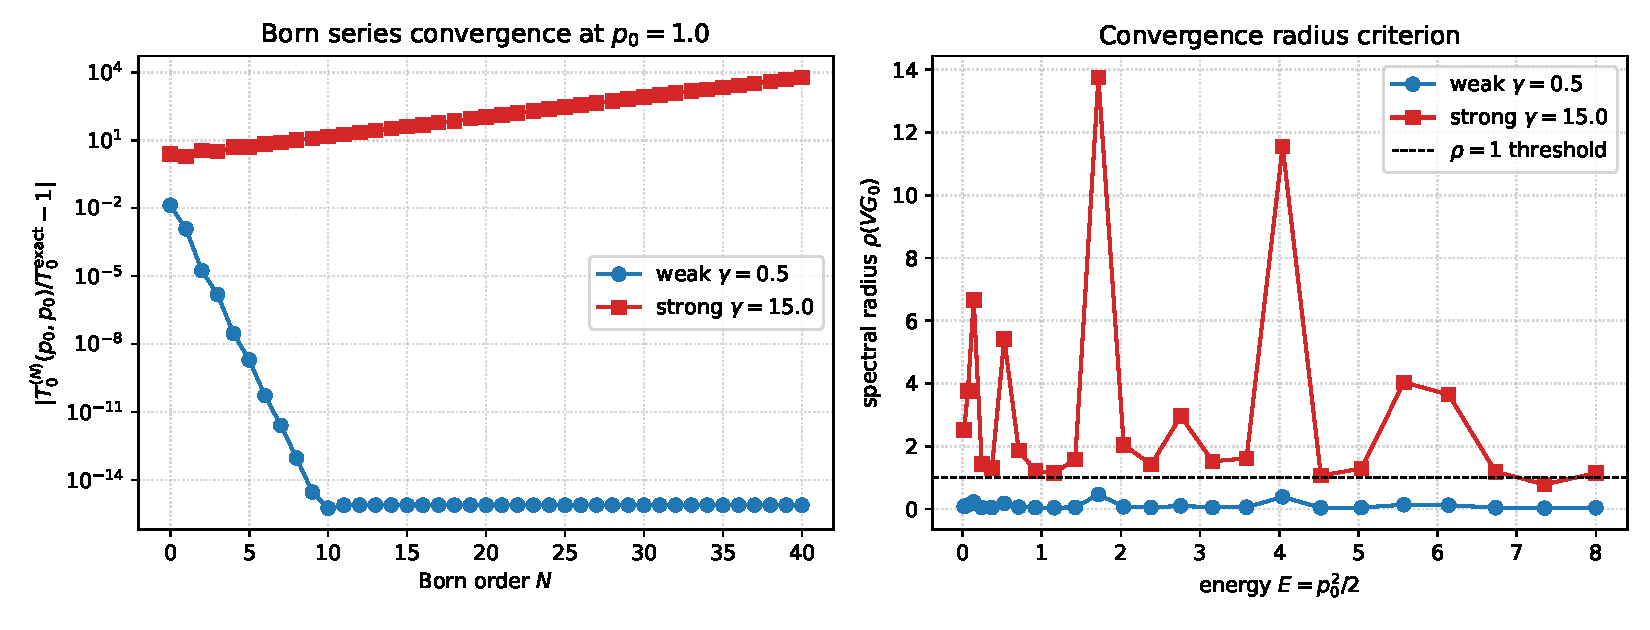
\includegraphics[width=0.95\linewidth]{ch08_born_convergence}
    \caption{Born 级数收敛性的数值验证. 左: $|T^{(N)}_{0}(p_{0},p_{0})/T_{0}^{\rm exact}-1|$
    随 Born 阶数 $N$ 的变化 (对数纵轴, $p_{0}=1$). 弱耦合 $\gamma=0.5$ (蓝色) 在 $N\sim 10$ 阶后
    达到机器精度; 强耦合 $\gamma=15$ (红色) 误差按几何方式 \emph{增大}, 表明 Born 级数发散.
    右: 算子 $VG^{0}$ 的谱半径 $\rho(VG^{0})$ 随能量 $E=p_{0}^{2}/2$ 的变化. 黑虚线为
    定理 $\rho<1$ 临界值. 弱耦合曲线一致地远在阈值之下; 强耦合曲线整体高于阈值, 且在某些能量
    出现尖峰——对应 $E$ 接近束缚态 / 共振极点时 $G^{0}$ 引起的奇异放大.}
    \label{fig:numexp-ch08}
\end{figure}

\subsection*{物理讨论}
\begin{enumerate}
\item \textbf{Born 收敛定理的数值验证.} 定理
\ref{thm:born-conv}: $\Vert VG^{0}\Vert<1$ $\Longrightarrow$ Neumann 级数
$\sum_{n}(VG^{0})^{n}$ 在算子范数下收敛. 数值实验中对应弱耦合
$\gamma=0.5$, 全能段 $\rho\sim 0.05\text{-}0.2$, 因此 $T^{(N)}\to T$ 几何收敛, 公比即谱半径——
图~\ref{fig:numexp-ch08} 左图斜率 $\log_{10}\rho\approx -0.7$ 与右图首点 $\rho_{w}\approx 0.18$
一致 (含离散化误差).
\item \textbf{束缚态阻碍全程收敛.} 强耦合 $\gamma=15$ 谱半径系统地 $>1$, 部分能量出现
$\rho\gg 1$ 的尖峰. 物理上: 当 $E$ 趋近某个束缚态能量 $E_{B}<0$ 的解析延拓投影时,
$G^{0}(p;E)$ 在被分立态 ``放大'' 的子空间贡献巨大本征值. 这与定理
\ref{thm:bound-state-block} (``束缚态阻碍 Born 级数全程收敛'') 一致, 也与本章一维 $\delta$
势例子 \eqref{eq:born-ex-delta-sum} 的几何级数公比 $\rmi mg/k$ 在 $|g|>k/m$ 时发散同源.
\item \textbf{收敛半径作为奇点指示器.} $\rho(VG^{0}(E))=1$ 的能量定义了 Born 级数的
\emph{收敛半径在能量平面上的边界}; 此边界即 $T(E)$ 作为 $E$ 的函数最近的奇点
(束缚态极点或 CDD 极点) 距离展开点的位置——这一观点正是 ch11 解析性、ch12
共振分析的出发点.
\item \textbf{重整化 / 重整求和的必要性.} 当 $\rho\geq 1$, 直接求 $T$ 必须求解线性方程
(\texttt{np.linalg.solve}) 而非作截断求和. 这正是核物理 / 多体散射中 Faddeev-AGS、
Padé 重整以及 ${\cal R}$-矩阵方法存在的根本原因: 对存在束缚 / 共振的系统, Born 级数
\emph{不是} 良定义的微扰展开.
\end{enumerate}

\chapter{定态散射理论 (Stationary Scattering)}\label{ch:stationary}

\section{从时间相关到时间无关的描述}

在前面几章中我们建立了散射问题的\emph{时间相关}（time-dependent）的表述：
入射态 $|\psi_{\text{in}}\rangle$ 在 $t\to-\infty$ 时趋于一个自由波包 $U_0(t)|\phi\rangle$；
经过相互作用区域以后，在 $t\to+\infty$ 时又趋于另外一个自由波包 $U_0(t)|\phi'\rangle$。
两组渐近态之间的变换矩阵正是散射 $\Smat$ 矩阵：
\begin{equation}
  \Smat = \Omega_-^\dagger\,\Omega_+\,,
  \qquad
  |\phi\pm\rangle \equiv \Omega_\pm |\phi\rangle\,.
\end{equation}
其中 $\Omega_\pm$ 是 M\o ller 算符（见第~\ref{ch:Smat1P}~章），它把可归一化的自由
渐近态 $|\phi\rangle$ 映成 $t=0$ 时刻真实的散射态 $|\phi\pm\rangle$。

入射波包和出射波包都可以用自由的能量本征态 $|\vec p\rangle$ 叠加得到：
\begin{equation}
  |\phi\rangle = \int \rmd^3 p\, \phi(\vec p)\,|\vec p\rangle\,,
\end{equation}
那么自然就提示我们对每一个动量本征态 $|\vec p\rangle$ 单独定义一个对应的``散射态''，
这便是\emph{定态散射态}（stationary scattering state）：
\begin{equation}
  \boxed{\;|\vec p\pm\rangle \;\equiv\; \Omega_\pm |\vec p\rangle\;.\;}
  \label{eq:def-ppm}
\end{equation}

由于 $|\vec p\rangle$ 不是可归一化的态，$|\vec p\pm\rangle$ 同样是 $\Hmat$ 的
\emph{improper} 本征矢，不具有有限的 norm。但它们可以作为完备的展开基，把任何
真实的散射态展开为它们的叠加。这就是所谓的\emph{时间无关的表述}：把全部散射信息
凝缩到一组能量本征态 $|\vec p\pm\rangle$ 当中，不再需要显式地考虑波包的时间演化。

历史上人们最早就是用时间无关的描述来处理散射问题。对球对称势散射，可以证明
（这正是本章要建立的渐近形式）
\begin{equation}
  \psi_+(\vec x) \;=\; \langle \vec x|\vec p+\rangle
  \;\xrightarrow{r\to\infty}\;
  (2\pi)^{-3/2}\!\left[\,\rme^{\rmi\vec p\cdot\vec x}
  + f(\theta,\varphi)\,\frac{\rme^{\rmi p r}}{r}\right].
  \label{eq:stationary-asymp-intro}
\end{equation}
通常的量子力学教材就是从这一渐近边界条件出发求解定态薛定谔方程，本章我们要把它
跟前几章建立的算符语言衔接起来。

求解 $|\vec p\pm\rangle$ 通常有两种途径：
\begin{itemize}
  \item \textbf{积分方程}：跟 Green 算符 $G(z)$、$\Tmat(z)$ 满足的 Lippmann--Schwinger
        方程相联系；
  \item \textbf{微分方程}：直接求解定态薛定谔方程 $\Hmat|\vec p\pm\rangle =
        E_p|\vec p\pm\rangle$，并加上适当的渐近边界条件。
\end{itemize}

\begin{remark}
后面用到的约定：$\hbar=1$（在最后给出 $f$ 与 $T$ 矩阵元的关系时再恢复 $\hbar$，
方便和教科书对照）；$E_p = \vec p^{\,2}/(2m)$；$|\vec p\rangle$ 取
$\langle \vec x|\vec p\rangle = (2\pi)^{-3/2}\rme^{\rmi\vec p\cdot\vec x}$，
$\inn{\vec p'}{\vec p} = \delta^3(\vec p'-\vec p)$。
\end{remark}

\section{$|\vec p\pm\rangle$ 的基本性质}

\subsection{是 $\Hmat$ 的本征态}

$|\vec p\rangle$ 是自由 Hamiltonian $\Hmat_0$ 的本征态，$\Hmat_0|\vec p\rangle =
E_p|\vec p\rangle$。利用 M\o ller 算符的 intertwining 关系
\begin{equation}
  \Hmat\,\Omega_\pm \;=\; \Omega_\pm\,\Hmat_0\,,
  \label{eq:intertwining}
\end{equation}
立刻得到
\begin{equation}
  \Hmat|\vec p\pm\rangle
  = \Hmat\Omega_\pm|\vec p\rangle
  = \Omega_\pm \Hmat_0|\vec p\rangle
  = E_p\,\Omega_\pm|\vec p\rangle
  = E_p\,|\vec p\pm\rangle\,.
  \label{eq:H-eigenppm}
\end{equation}
即 $|\vec p\pm\rangle$ 是真实 Hamiltonian $\Hmat$ 的 improper 本征态，本征值
$E_p = \vec p^{\,2}/(2m)$ 跟自由渐近态 $|\vec p\rangle$ 完全一致。

\subsection{时间演化与 $t\to\mp\infty$ 渐近行为}

由于 $|\vec p\pm\rangle$ 是 $\Hmat$ 的本征态，
\begin{equation}
  U(t)|\vec p\pm\rangle \;=\; \rme^{-\rmi E_p t}|\vec p\pm\rangle\,,
  \qquad
  U_0(t)|\vec p\rangle \;=\; \rme^{-\rmi E_p t}|\vec p\rangle\,.
\end{equation}
注意它们随时间只是带一个总相位 $\rme^{-\rmi E_p t}$ ——所以从单个 $|\vec p\pm\rangle$
本身\emph{看不出}它在 $t\to\mp\infty$ 时趋于自由的 $|\vec p\rangle$！这正是
$|\vec p\pm\rangle$ 不是物理的可归一化态导致的``失真''。

要恢复时间相关的描述，必须做\emph{波包平滑（smearing）}。对一可归一化的 $\phi$，
$|\phi\pm\rangle = \int\!\rmd^3p\,\phi(\vec p)\,|\vec p\pm\rangle$，那么
\begin{equation}
  U(t)|\phi\pm\rangle
  = \int\!\rmd^3p\,\phi(\vec p)\,U(t)|\vec p\pm\rangle
  \;\xrightarrow{t\to\mp\infty}\;
  \int\!\rmd^3p\,\phi(\vec p)\,U_0(t)|\vec p\rangle
  = U_0(t)|\phi\rangle\,,
\end{equation}
回到了 M\o ller 算符的定义关系 $\lim_{t\to\mp\infty}U_0(-t)U(t)|\phi\pm\rangle =
|\phi\rangle$。在 smear 过的意义下我们也可以说：``入射（出射）渐近态
$|\vec p\rangle$ 对应的散射态在 $t=0$ 时刻是 $|\vec p+\rangle$（$|\vec p-\rangle$）''。

\subsection{完备性与正交归一}

由于 $\Omega_\pm$ 把 $\Hilb_{\text{free}}$ 等距映到 $\Hilb$ 中渐近完备的子空间
$\mathcal{R}=\Ran(\Omega_\pm)$，且 $\Omega_\pm^\dagger\Omega_\pm = \mathbf{1}$，
所以 $\{|\vec p\pm\rangle\}$ 在 $\mathcal{R}$ 上是正交完备的：
\begin{equation}
  \inn{\vec p'\pm}{\vec p\pm}
  = \matel{\vec p'}{\Omega_\pm^\dagger\Omega_\pm}{\vec p}
  = \delta^3(\vec p'-\vec p)\,.
  \label{eq:ppm-ortho}
\end{equation}

由渐近完备性 $\Hilb = \mathcal{R}\oplus\mathcal{B}$，其中 $\mathcal{B}$ 是束缚态张
成的子空间，所以 $\{|\vec p+\rangle\}\cup\{|n\rangle_{\text{bound}}\}$（同样
$\{|\vec p-\rangle\}\cup\{|n\rangle\}$）构成 $\Hilb$ 的一组完备基矢：
\begin{align}
  \mathbf{1}
  &= \int\!\rmd^3p\,|\vec p\rangle\langle\vec p|
   = \int\!\rmd^3p\,|\vec p+\rangle\langle\vec p+|+\sum_n |n\rangle\langle n|\nonumber\\
  &= \int\!\rmd^3p\,|\vec p-\rangle\langle\vec p-|+\sum_n |n\rangle\langle n|\,.
  \label{eq:completeness}
\end{align}
注意 $|\vec p+\rangle$ 和 $|\vec p-\rangle$ 都是同一个 $\Hmat$ 在同一本征值
$E_p$ 上的本征矢，意味着实际的能量本征空间是\emph{高度简并}的（既有 ``in'' 标记，
也有 ``out'' 标记，简并的方向数对应 $4\pi$ 立体角）。

\section{定态散射态满足的积分方程}

\subsection{用 $G$ 写的 Lippmann--Schwinger 方程}

第~\ref{ch:green}~章已经导出，对可归一化的态 $|\phi\rangle$，
\begin{equation}
  |\phi\pm\rangle \;=\; |\phi\rangle + \int\!\rmd^3 p\,
  G(E_p\pm \rmi\epsilon)\,\Vmat\,|\vec p\rangle\,\langle \vec p|\phi\rangle\,.
  \label{eq:LS-phipm}
\end{equation}
左右两边把 $|\phi\pm\rangle$ 和 $|\phi\rangle$ 用 $|\vec p\pm\rangle$、
$|\vec p\rangle$ 展开，$|\phi\rangle = \int\rmd^3 p\,\phi(\vec p)|\vec p\rangle$，
$|\phi\pm\rangle = \int\rmd^3 p\,\phi(\vec p)|\vec p\pm\rangle$，则
\begin{equation}
  \int\!\rmd^3 p\,\phi(\vec p)\,|\vec p\pm\rangle
  = \int\!\rmd^3 p\,\phi(\vec p)\Big(|\vec p\rangle
    + G(E_p\pm \rmi\epsilon)\,\Vmat\,|\vec p\rangle\Big)\,.
\end{equation}
由于这对任意 $\phi(\vec p)$ 都成立，被积函数必须相等，于是
\begin{equation}
  \boxed{\;|\vec p\pm\rangle \;=\; |\vec p\rangle
  + G(E_p\pm \rmi\epsilon)\,\Vmat\,|\vec p\rangle\;.\;}
  \label{eq:LS-G-ch09}
\end{equation}
这是定态散射态的 Lippmann--Schwinger 方程的第一种形式。$\pm \rmi\epsilon$ 处方
分别选取了出射（incoming wave at infinity is plane wave only, plus outgoing
spherical wave）和入射（plus incoming spherical wave）边界条件。

\subsection{用 $G_0$ 写的 Lippmann--Schwinger 方程}

利用 $GV = G_0 T$（见第~\ref{ch:green}~章），\eqref{eq:LS-G-ch09} 可以等价地用
自由 Green 算符 $G_0$ 写出：
\begin{equation}
  \boxed{\;|\vec p\pm\rangle \;=\; |\vec p\rangle
  + G_0(E_p\pm \rmi\epsilon)\,\Vmat\,|\vec p\pm\rangle\;.\;}
  \label{eq:LS-G0}
\end{equation}
这就是大多数教科书写下的 \emph{Lippmann--Schwinger 方程}。它是 $|\vec p\pm\rangle$
的隐式积分方程，可迭代得到 Born 级数：
\begin{equation}
  |\vec p+\rangle = |\vec p\rangle + G_0(E_p+\rmi 0)\Vmat|\vec p\rangle
  + G_0(E_p+\rmi 0)\Vmat G_0(E_p+\rmi 0)\Vmat|\vec p\rangle + \cdots\,.
  \label{eq:Born-state}
\end{equation}
此时我们手中已经有三个相互等价的 Lippmann--Schwinger 方程：
\begin{align}
  (1-G_0\Vmat)\,G &= G_0\,,\label{eq:LS-G-ch09-op}\\
  (1-\Vmat G_0)\,T &= \Vmat\,,\label{eq:LS-T-ch09}\\
  (1-G_0\Vmat)\,|\vec p\pm\rangle &= |\vec p\rangle\,.\label{eq:LS-state-op}
\end{align}

\subsection{壳上 $T$-矩阵元}

把 $T(z) = \Vmat + \Vmat G(z)\Vmat$ 作用到 $|\vec p\rangle$ 上：
\begin{equation}
  T(E_p\pm \rmi 0)|\vec p\rangle
  = \big[\Vmat + \Vmat G(\pm)\Vmat\big]|\vec p\rangle
  = \Vmat\big[\,\mathbf{1}+G(\pm)\Vmat\,\big]|\vec p\rangle
  = \Vmat\,|\vec p\pm\rangle\,.
  \label{eq:T-on-p}
\end{equation}
取左矢 $\langle\vec p'|$ 得到
\begin{equation}
  \boxed{\;t(\vec p'\leftarrow \vec p) \;\equiv\; \langle\vec p'|T(E_p+\rmi 0)|\vec p\rangle
  \;=\; \langle\vec p'|\Vmat|\vec p+\rangle\;.\;}
  \label{eq:t-onshell-1}
\end{equation}
这就是我们在前面章节频繁使用的\emph{在壳} $T$-矩阵元（``on-shell''指 $|\vec p|=
|\vec p'|$，但 $T$ 中能量参数取在 $E_p+\rmi 0$，与初态动能匹配）。

利用 $T(z)^\dagger = T(z^*)$，
\begin{equation}
  \langle\vec p'|T(E_{p'}+\rmi 0) = \langle\vec p' -|\Vmat
  \;\;\Longrightarrow\;\;
  t(\vec p'\leftarrow \vec p) = \langle\vec p'-|\Vmat|\vec p\rangle\,.
  \label{eq:t-onshell-2}
\end{equation}
两种写法在壳（$E_{p'}=E_p$）时一致。配合 \eqref{eq:Born-state} 立刻有
\begin{equation}
  t(\vec p'\leftarrow \vec p)
  = \langle\vec p'|\Vmat|\vec p\rangle
  + \langle\vec p'|\Vmat G_0\Vmat|\vec p\rangle + \cdots\,,
\end{equation}
即 $T$-矩阵元的 Born 展开。

\section{坐标表象的定态波函数}

\subsection{积分方程}

把 \eqref{eq:LS-G0} 投影到坐标 $\langle\vec x|$，并在中间插入完备性
$\int\rmd^3 x'\,|\vec x'\rangle\langle\vec x'|$：
\begin{equation}
  \langle\vec x|\vec p\pm\rangle
  = \langle\vec x|\vec p\rangle
  + \int\!\rmd^3 x'\,\langle\vec x|G_0(E_p\pm\rmi\epsilon)|\vec x'\rangle\,
    V(\vec x')\,\langle\vec x'|\vec p\pm\rangle\,.
  \label{eq:LS-coord}
\end{equation}
（这里假设 $V$ 在坐标表象是局域的：$\langle\vec x|\Vmat|\vec x'\rangle =
V(\vec x)\,\delta^3(\vec x-\vec x')$。）这就是教科书上熟悉的、关于波函数
$\psi^\pm(\vec x) \equiv \langle\vec x|\vec p\pm\rangle$ 的积分方程。

\subsection{自由 Green 函数 $\langle\vec x|G_0(z)|\vec x'\rangle$}

需要 $G_0(z)$ 的坐标表象。利用动量基插入完备性，
\begin{align}
  \langle\vec x|G_0(z)|\vec x'\rangle
  &= \int\!\rmd^3 p\,\frac{\langle\vec x|\vec p\rangle\langle\vec p|\vec x'\rangle}{z-E_p}
   = \frac{1}{(2\pi)^3}\int\!\rmd^3 p\,
     \frac{\rme^{\rmi \vec p\cdot(\vec x-\vec x')}}{z-\vec p^{\,2}/(2m)}\nonumber\\
  &= \frac{1}{(2\pi)^3}\int_0^\infty\! p^2\rmd p\int\rmd\Omega_p\,
     \frac{\rme^{\rmi p|\vec x-\vec x'|\cos\theta}}{z-p^2/(2m)}\nonumber\\
  &= \frac{-\rmi}{4\pi^2|\vec x-\vec x'|}\int_0^\infty p\,\rmd p\,
     \frac{\rme^{\rmi p|\vec x-\vec x'|}-\rme^{-\rmi p|\vec x-\vec x'|}}{z-p^2/(2m)}\nonumber\\
  &= \frac{\rmi m}{4\pi^2|\vec x-\vec x'|}\int_{-\infty}^{\infty}\rmd p\,
     \frac{p\,\rme^{\rmi p|\vec x-\vec x'|}}{p^2-2mz}\,.
\end{align}
对最后一行作 $p$-平面回路（沿上半平面闭合）求复变积分。$z$ 上方有一对极点
$p=\pm(2mz)^{1/2}$；按照 $\Im (2mz)^{1/2}>0$ 选取根号支，则上半平面上的极点是
$p_+ = +(2mz)^{1/2}$。由留数定理得
\begin{equation}
  \langle\vec x|G_0(z)|\vec x'\rangle
  = -\frac{m}{2\pi}\,\frac{\exp\!\big[\rmi(2mz)^{1/2}|\vec x-\vec x'|\big]}{|\vec x-\vec x'|}\,,
  \qquad \Im(2mz)^{1/2}>0\,.
  \label{eq:G0-coord}
\end{equation}

把 $z = E_p\pm\rmi 0$ 代入。由 $E_p = p^2/(2m)$，$(2mz)^{1/2}\to \pm p+\rmi 0$
（注意 $-$ 号选 ``$+\rmi 0$'' 时根号支变 $-p+\rmi 0$，同样保证 $\Im>0$）。所以
\begin{equation}
  \langle\vec x|G_0(E_p\pm\rmi 0)|\vec x'\rangle
  = -\frac{m}{2\pi}\,\frac{\rme^{\pm \rmi p|\vec x-\vec x'|}}{|\vec x-\vec x'|}\,.
  \label{eq:G0-eps}
\end{equation}
代回 \eqref{eq:LS-coord}，
\begin{equation}
  \langle\vec x|\vec p\pm\rangle
  = \langle\vec x|\vec p\rangle
  - \frac{m}{2\pi}\int\!\rmd^3 x'\,
    \frac{\rme^{\pm \rmi p|\vec x-\vec x'|}}{|\vec x-\vec x'|}\,V(\vec x')\,
    \langle\vec x'|\vec p\pm\rangle\,.
  \label{eq:LS-coord-explicit}
\end{equation}
\eqref{eq:LS-coord-explicit} 就是定态波函数 $\psi^\pm(\vec x)$ 满足的具体积分
方程。$+$ 号对应 \emph{outgoing}（出射球面波）边界，$-$ 号对应 \emph{incoming}
（入射球面波）边界。

\begin{remark}
回路选择的物理含义：$\rme^{+\rmi p|\vec x-\vec x'|}$ 跟 $\rme^{-\rmi E_p t}$ 配
合得到 $\rme^{\rmi(pr-E_p t)}$，这是\emph{向外}（指向 $\vec x$ 远离 $\vec x'$ 方
向）传播的球面波；反之 $-$ 号给出向内传播的球面波。这与下一节渐近形式的物理含义
完全一致。
\end{remark}

\subsection{大 $r$ 渐近形式与散射振幅}

假设势是有限程的：$V(\vec r)=0$ 当 $r>a$。考察大 $r$（$r\to\infty$、$r\gg a$）
区域的 $\langle\vec x|\vec p\pm\rangle$：积分中 $r'\le a$，因此可以做远场展开
\begin{equation}
  |\vec x-\vec x'| = \big(r^2 - 2\vec x\cdot\vec x' + r'^2\big)^{1/2}
  = r\Big[1 - \frac{\vec x\cdot\vec x'}{r^2} + O\!\Big(\frac{r'}{r}\Big)^2\Big]
  = r - \hat{\vec x}\cdot\vec x' + O\!\Big(\frac{r'^{\,2}}{r}\Big)\,,
\end{equation}
其中 $\hat{\vec x}=\vec x/r$。代入 \eqref{eq:LS-coord-explicit}，
\begin{equation}
  \langle\vec x|\vec p\pm\rangle
  = \langle\vec x|\vec p\rangle
  - \frac{m\,\rme^{\pm \rmi p r}}{2\pi r}\int\!\rmd^3 x'\,
    \rme^{\mp \rmi p\hat{\vec x}\cdot\vec x'}\,V(\vec x')\,
    \langle\vec x'|\vec p\pm\rangle
    \!\left[1+O\!\Big(\frac{a}{r}\Big)+O\!\Big(\frac{p a^2}{r}\Big)\right]\!.
\end{equation}
注意被积分的部分恰好是 \eqref{eq:t-onshell-2} 的逆：定义出射/入射方向的动量
$\vec p'\equiv \pm p\hat{\vec x}$（$+$对$+$，$-$对$-$），则
\begin{equation}
  \int\!\rmd^3 x'\,\rme^{\mp \rmi p\hat{\vec x}\cdot\vec x'}V(\vec x')
  \langle\vec x'|\vec p\pm\rangle
  = (2\pi)^{3/2}\,\langle \pm p\hat{\vec x}|\Vmat|\vec p\pm\rangle
  = (2\pi)^{3/2}\,t(\pm p\hat{\vec x}\leftarrow \vec p)\,.
\end{equation}
因此
\begin{equation}
  \langle\vec x|\vec p\pm\rangle
  \;\xrightarrow{r\to\infty}\;
  (2\pi)^{-3/2}\!\left[\rme^{\rmi\vec p\cdot\vec x}
  \;-\;(2\pi)^2 m\,\langle \pm p\hat{\vec x}|\Vmat|\vec p\pm\rangle\,
  \frac{\rme^{\pm\rmi p r}}{r}\right]\!.
  \label{eq:asymp-derived}
\end{equation}
与教科书中标准的渐近边界条件
\begin{equation}
  \psi^\pm(\vec x)\;\xrightarrow{r\to\infty}\;
  (2\pi)^{-3/2}\!\left[\rme^{\rmi\vec p\cdot\vec x}
  + f(p\hat{\vec x}\leftarrow\vec p)\,\frac{\rme^{\pm\rmi p r}}{r}\right]
  \label{eq:asymp-textbook}
\end{equation}
对比，立得
\begin{empheq}[box=\fbox]{equation}
  f(\vec k'\leftarrow \vec k) \;=\; -\,(2\pi)^2 m\,\langle\vec k'|\Vmat|\vec k+\rangle
  \;=\; -\,(2\pi)^2 m\,\langle\vec k'|T(E_k+\rmi 0)|\vec k\rangle\,.
  \label{eq:f-T-relation}
\end{empheq}
这正是\emph{从定态图像直接定义散射振幅与 $T$-矩阵元的关系}。在恢复 $\hbar$ 后
（$\vec p\to\hbar\vec k$，$\rmd^3p\to\hbar^3\rmd^3k$，$E=\hbar^2 k^2/(2m)$），上式
按通常的写法就是
\begin{equation}
  \boxed{\;f(\vec k'\leftarrow \vec k)
  \;=\; -\,\frac{(2\pi)^2 m}{\hbar^2}\,\langle\vec k'|\Tmat|\vec k\rangle\,.\;}
  \label{eq:f-T-hbar}
\end{equation}

\eqref{eq:asymp-derived}--\eqref{eq:f-T-relation} 同时实现了三件事情：
\begin{enumerate}
  \item 重新导出了教科书的渐近边界条件 \eqref{eq:asymp-textbook}，确认
        $\langle\vec x|\vec p\pm\rangle$ 在大 $r$ 处确实是``平面波 + 出射/入射
        球面波''；
  \item 把渐近振幅 $f$ 与算符语言下的在壳 $T$-矩阵元 $\langle\vec k'|T|\vec k\rangle$
        显式联系起来；
  \item 完成了\emph{时间相关}与\emph{时间无关}两种散射表述的等价性证明。
\end{enumerate}

\subsection{物理解读}

\eqref{eq:asymp-textbook} 中的两个解 $\psi^+$、$\psi^-$ 物理含义清晰：
\begin{itemize}
  \item $\psi^+ = \langle\vec x|\vec p+\rangle$：``in'' 态——平面波入射，加上一个
        \emph{出射}的球面波 $f\,\rme^{\rmi p r}/r$。这正是真实散射实验所对应的
        定态散射波函数。
  \item $\psi^- = \langle\vec x|\vec p-\rangle$：``out'' 态——平面波加上一个
        \emph{入射}的球面波 $f^{(-)}\,\rme^{-\rmi pr}/r$。在 LSZ 类型的论证（散射
        振幅的对偶表达）中会用到。
\end{itemize}

\section{时间无关表述：常见教科书做法}

许多量子力学教材的``正统''顺序是：
\begin{enumerate}
  \item \textbf{设 ansatz}：在无穷远处定态波函数取
        \eqref{eq:asymp-textbook} 的边界条件，从中读出散射振幅 $f$；
  \item \textbf{物理诠释}：平面波代表入射粒子流，球面波代表散射出去的粒子；用入
        射流密度归一，出射粒子单位时间单位立体角的数目除以入射通量给出微分散射
        截面
        \begin{equation}
          \frac{\rmd\sigma}{\rmd\Omega} = |f(\theta,\varphi)|^2\,;
          \label{eq:dsig-dOmega}
        \end{equation}
  \item \textbf{解方程}：把带有渐近边界条件的定态薛定谔方程 $(\Hmat-E_p)\psi=0$
        化为 \eqref{eq:LS-coord-explicit} 形式的积分方程，再化为 Lippmann--
        Schwinger 算符方程 \eqref{eq:LS-G0}，最终得到
        \begin{equation}
          f(\vec k'\leftarrow\vec k) = -(2\pi)^2 m\,\langle\vec k'|\Vmat|\vec k+\rangle\,;
        \end{equation}
        迭代求解再得到 Born 级数。
\end{enumerate}

我们前面的处理顺序则是反过来的：先有时间相关 + M\o ller 算符的语言，再定义
$|\vec p\pm\rangle$，最后从大 $r$ 渐近导出 \eqref{eq:asymp-textbook}。两条路径
在物理与数学上完全等价。

\begin{remark}[关于 $|\vec p\pm\rangle$ 的非物理性]
$|\vec p\pm\rangle$ 没有有限的 norm，不是物理可实现的态，是 $\Hmat$ 的 improper
本征态——这跟自由情形 $|\vec p\rangle$ 的地位完全相同。它们的作用是\emph{展开
基}：真实可归一的散射态在 $t=0$ 处可写成
\begin{equation}
  |\psi\rangle = |\phi+\rangle = \int\!\rmd^3p\,\phi(\vec p)\,|\vec p+\rangle\,,
  \qquad
  |\psi_{\text{in}}\rangle = \int\!\rmd^3p\,\phi(\vec p)\,|\vec p\rangle\,,
\end{equation}
两组展开系数 $\phi(\vec p)$ \emph{完全相同}。当 $\phi(\vec p)$ 集中在某一 $\vec
p_0$ 附近的极窄动量区间时，$\psi_{\text{in}}$ 趋近于一个准单色平面波，散射态的
物理性质就由 $|\vec p_0+\rangle$ 这一个本征态完全给出。
\end{remark}

\section{用波包恢复散射的坐标空间描述}

之前算微分散射截面是在动量空间中数 $\rmd\Omega$ 立体角内出射的粒子数
$N_{\text{sc}}(\rmd\Omega)$；为了把 \eqref{eq:dsig-dOmega} 跟实验中粒子计数器在
空间某方向上探测到的粒子数直接联系起来，需要在坐标空间中重新论证一遍。这里要结合
\eqref{eq:asymp-textbook} 的渐近形式来分析时间相关的波函数。

\subsection{波包的时间演化}

设入射波包 $\phi(\vec p)$ 集中在 $\vec p_0$ 附近、宽度 $\Delta p$，$\hat{\vec
p}_0$ 沿 $\hat{\vec 3}$ 方向。在 $t<-t_0$（即碰撞尚未发生）时入射波包
\begin{align}
  \psi_{\text{in}}(\vec x,t)
  &= \langle\vec x|U_0(t)|\psi_{\text{in}}\rangle
   = (2\pi)^{-3/2}\int\!\rmd^3 p\,\phi(\vec p)\,\rme^{\rmi(\vec p\cdot\vec x-E_p t)}\,.
\end{align}
群速度 $\vec v_0 = \vec p_0/m$。把指数中 $E_p$ 在 $\vec p_0$ 处展开
$E_p = E_0 + \vec v_0\cdot(\vec p-\vec p_0) + O(\Delta p^2/m)$，可以写出
\begin{equation}
  \psi_{\text{in}}(\vec x,t) = \rme^{\rmi E_0 t}\,\psi_{\text{in}}(\vec x-\vec v_0 t,0)
  \!\left[1+O\!\Big(\frac{\Delta p^2 t}{m}\Big)\right]\!.
  \label{eq:packet-shift}
\end{equation}
即在时间尺度 $t\ll mb^2$（$b\sim 1/\Delta p$ 是波包横向尺度）内，波包按群速度
$\vec v_0$ 平移而不显著弥散。

\subsection{$t>0$ 的散射波}

设 $t=0$ 时波包刚好抵达靶子（取靶子为坐标原点）。$t > -(b+a)/v_0$ 后粒子已经感受
到靶的相互作用，必须用真实演化 $U(t)|\psi\rangle$ 来描述：
\begin{equation}
  \psi(\vec x,t) = \langle\vec x|U(t)|\psi\rangle
  = \int\!\rmd^3 p\,\phi(\vec p)\,\rme^{-\rmi E_p t}\,\langle\vec x|\vec p+\rangle\,.
\end{equation}
对探测器位置 $\vec x = r\hat{\vec x}$，$r\gg a$、$r\gg p_0 a^2$，把
$\langle\vec x|\vec p+\rangle$ 替换成它的渐近形式 \eqref{eq:asymp-textbook}：
\begin{align}
  \psi(\vec x,t)
  &\xrightarrow{r\to\infty}\;
  (2\pi)^{-3/2}\int\!\rmd^3p\,\phi(\vec p)\,\rme^{-\rmi E_p t}
  \!\left[\rme^{\rmi\vec p\cdot\vec x}
  + f(p\hat{\vec x}\leftarrow\vec p)\,\frac{\rme^{\rmi pr}}{r}\right]\nonumber\\
  &= \psi_{\text{in}}(\vec x,t) + \psi_{\text{sc}}(\vec x,t)\,.
\end{align}
即在远离靶子处，全波函数自动分成入射波包加散射波。

由于 $\phi(\vec p)$ 集中在 $\vec p_0$ 附近，且通常 $b\gg a$ 使 $f$ 在 $\vec p_0$
附近变化比 $\phi$ 慢得多，$f$ 可提到积分外：
\begin{align}
  \psi_{\text{sc}}(\vec x,t)
  &\xrightarrow{r\to\infty}\;
  \frac{f(p_0\hat{\vec x}\leftarrow \vec p_0)}{r}
  \int\!\rmd^3 p\,\phi(\vec p)\,\rme^{\rmi(p r - E_p t)}\nonumber\\
  &\xrightarrow{p r\,\approx\, \vec p\cdot \hat{\vec x}\, r}\;
  \frac{f(p_0\hat{\vec x}\leftarrow \vec p_0)}{r}\,
  \psi_{\text{in}}(r\hat{\vec x},t)\!\left[1+O\!\Big(\frac{r}{p_0 b^2}\Big)\right]\!.
  \label{eq:psi-sc}
\end{align}
\eqref{eq:psi-sc} 显示：散射波在远场处可以视作沿径向 $\hat{\vec x}$ 方向以群速度
传播的球面波，其``形状''与入射波包相同，只是加权了一个角度依赖因子 $f/r$。

\subsection{微分散射截面}

假设探测器不放在没有发生散射的原入射粒子路径上，即 $d\sin\theta\gg b$，
则探测到一个粒子的总概率
\begin{align}
  w(\rmd\Omega\leftarrow\phi)
  &= \rmd\Omega\int_0^\infty\rmd r\,r^2\,|\psi_{\text{sc}}(\vec x,t)|^2\nonumber\\
  &= \rmd\Omega\,|f(\vec p_0\leftarrow\vec p_0)|^2
     \int_{-\infty}^{\infty}\rmd r\,|\psi_{\text{in}}(r\hat{\vec 3},t)|^2\,.
  \label{eq:w}
\end{align}
（积分下限取到 $-\infty$，因为入射波包在 $z<0$、$t$ 较大时已经几乎为零，对积分
没贡献。）

一个真实的实验要对许多次入射、不同的碰撞参数 $\vec\rho$ 求平均（$\vec\rho$ 是
入射方向横向的位移），即对 $\rmd^2\rho$ 积分，得到微分散射截面
\begin{align}
  \sigma(\rmd\Omega\leftarrow\phi)
  &= \int\!\rmd^2\rho\,w(\rmd\Omega\leftarrow\phi)\nonumber\\
  &= |f(\vec p_0\leftarrow\vec p_0)|^2\,
     \int\!\rmd^2\rho\int_{-\infty}^{\infty}\rmd r\,|\psi_{\text{in}}(r\hat{\vec 3}-\vec\rho,t)|^2\nonumber\\
  &= |f(\vec p_0\leftarrow\vec p_0)|^2\,\rmd\Omega\int\!\rmd^3 x\,|\psi_{\text{in}}(\vec x,t)|^2\nonumber\\
  &= |f(\vec p_0\leftarrow\vec p_0)|^2\,\rmd\Omega\,,
  \label{eq:dsig-final}
\end{align}
其中末步用了 $\psi_{\text{in}}$ 的归一化 $\int|\psi_{\text{in}}|^2\rmd^3x=1$。
这就重新得到 \eqref{eq:dsig-dOmega}：$\rmd\sigma/\rmd\Omega = |f|^2$，且与上一章
基于 $\Smat$-矩阵和波包在动量空间的论证完全一致——它们就是同一物理量的两种等价
表达。

\subsection{各种近似条件的相容性}

整个论证用到了如下近似：
\begin{itemize}
  \item 波包在碰撞过程中不显著弥散：$t/(mb^2)\sim v_0 t/(p_0 b^2)\ll 1$，即
        $d=v_0 t\ll p_0 b^2$；
  \item 渐近边界条件 \eqref{eq:asymp-textbook} 适用：$d\gg a$、$d\gg p a^2$；
  \item 波包窄于势的散射变化尺度：$a\ll b$；
  \item $f$ 几乎不变：$d\ll p_0 b^2$；
  \item 探测器避开未散射的束流：$d\sin\theta\gg b$。
\end{itemize}
所有条件归结成一个长不等式：
\begin{equation}
  \boxed{\;a \;\ll\; b \;\ll\; d \;\ll\; p_0 b^2\,,
  \qquad p_0 a^2 \;\ll\; d\,.\;}
  \label{eq:length-hier}
\end{equation}

\begin{example}[典型实验数量级]
考虑 10\,eV 电子（$p\sim 10^{10}\,\text{m}^{-1}$）束 $b\sim 10^{-3}$\,m，与
原子散射 $a\sim 10^{-10}$\,m，探测器距离 $d\sim 1$\,m：
\begin{equation*}
  10^{-10}\;\ll\;10^{-3}\;\ll\;1\;\ll\;10^{4}\,(\text{m})\,,
  \qquad 10^{-10}\;\ll\;1\,(\text{m})\,,
\end{equation*}
不等式 \eqref{eq:length-hier} 都很好地满足。
\end{example}

\section{光学定理（Optical theorem）}

定态形式给出了导出光学定理的简洁路径。从 $\Smat$ 的幺正性
$\Smat^\dagger\Smat = \mathbf{1}$ 出发，写
$\Smat = \mathbf{1} - 2\pi\rmi\,\delta(E_{p'}-E_p)\,T(\vec p'\leftarrow\vec p)$
（见第~\ref{ch:green}~章），可得
\begin{equation}
  T-T^\dagger = -2\pi\rmi\,T\,\delta(\Hmat_0-E)\,T^\dagger\,,
  \label{eq:T-unitarity}
\end{equation}
取对角矩阵元 $\langle\vec p|\cdots|\vec p\rangle$（$|\vec p'|=|\vec p|=k$，
$E_p=E$），左边
\begin{equation}
  \langle\vec p|T-T^\dagger|\vec p\rangle = 2\rmi\,\Im\langle\vec p|T|\vec p\rangle\,;
\end{equation}
右边
\begin{equation}
  -2\pi\rmi\!\int\!\rmd^3p''\,\delta(E_{p''}-E)\,
     |\langle\vec p''|T|\vec p\rangle|^2
   = -2\pi\rmi\,\frac{m k}{1}\!\int\rmd\Omega''\,
     |\langle\vec p''|T|\vec p\rangle|^2\,,
\end{equation}
（用 $\rmd^3p'' = p''^2\rmd p''\rmd\Omega''$，$\delta(E_{p''}-E)\rmd p'' =
m\rmd p''/p''$ 在 $p''=k$ 处）。代入 \eqref{eq:f-T-hbar}：
$\langle\vec p''|T|\vec p\rangle = -f/[(2\pi)^2 m]$，于是
\begin{equation}
  2\rmi\,\Im\langle\vec p|T|\vec p\rangle
  = -2\pi\rmi\,m k\,\frac{1}{(2\pi)^4 m^2}\!\int\!\rmd\Omega''\,|f|^2\,.
\end{equation}
再用 $\sigma_{\text{tot}} = \int\rmd\Omega''\,|f|^2$ 和 $\Im f(0) =
-(2\pi)^2 m\,\Im\langle\vec p|T|\vec p\rangle$（前向 $\vec p''=\vec p$），整理后
得到
\begin{empheq}[box=\fbox]{equation}
  \Im f(\theta=0) \;=\; \frac{k}{4\pi}\,\sigma_{\text{tot}}\,.
  \label{eq:optical}
\end{empheq}
这就是光学定理。它的物理含义是：前向散射振幅的虚部正比于总截面，反映了入射粒子
被散射``走''之后前向波幅必须减弱（概率守恒）。

\begin{remark}
光学定理 \eqref{eq:optical} 仅依赖 $\Smat$ 的幺正性（即概率守恒），与势 $V$ 是否
为厄米的具体形式无关；只要 $V=V^\dagger$ 它就成立。在含吸收（光学势 $\Im V<0$）
情形下，公式右边对应弹性 + 反应总截面之和。
\end{remark}

\section{小结}

本章把时间相关与时间无关两种散射表述桥接起来：
\begin{enumerate}
  \item 通过 \eqref{eq:def-ppm} 定义定态散射态 $|\vec p\pm\rangle = \Omega_\pm
        |\vec p\rangle$，它们是 $\Hmat$ 的 improper 本征态，本征值 $E_p$；
  \item 它们满足 Lippmann--Schwinger 积分方程 \eqref{eq:LS-G-ch09}/\eqref{eq:LS-G0}，
        可以用 Born 级数迭代求解；
  \item 在壳 $T$-矩阵元 $\langle\vec p'|T(E_p+\rmi 0)|\vec p\rangle =
        \langle\vec p'|\Vmat|\vec p+\rangle$，跟散射振幅的关系是
        \eqref{eq:f-T-hbar}：$f = -(2\pi)^2 m\,\langle\vec k'|T|\vec k\rangle/\hbar^2$；
  \item 坐标表象的波函数 \eqref{eq:LS-coord-explicit} 在大 $r$ 处自动给出
        ``平面波 + 出射/入射球面波'' 的渐近形式 \eqref{eq:asymp-textbook}，
        从而恢复教科书的标准定义；
  \item 借助波包平滑可以重建坐标空间的散射截面 $\rmd\sigma/\rmd\Omega = |f|^2$，
        并得到一组合理的尺度不等式 \eqref{eq:length-hier}；
  \item 由 $\Smat$ 的幺正性导出光学定理 $\Im f(0) = (k/4\pi)\sigma_{\text{tot}}$。
\end{enumerate}
这些结果将作为下一章\emph{分波法}（partial-wave expansion）以及后续解析性、共振
讨论的基础。

% =====================================================================
\section{本章定理证明补全}\label{sec:stat-proofs}

前面正文给出的多个结论中，有几个关键命题在严格性方面值得做更细致的展开：
\begin{itemize}
  \item M\o ller 算符语言下的 $|\vec p\pm\rangle$（时间相关图像）与教科书定义的、
        满足 \eqref{eq:asymp-textbook} 渐近边界条件的定态散射波函数（时间无关图像）
        ——\emph{为何} 是同一个对象？
  \item 从 Lippmann--Schwinger 积分方程 \eqref{eq:LS-coord-explicit} 得到大 $r$
        渐近形式时，远场展开的合法性、误差量级如何严格控制？
  \item 光学定理 $\Im f(0) = (k/4\pi)\sigma_{\rm tot}$ 究竟在 $\Smat$ 幺正性的什么
        意义下成立？
\end{itemize}
本节集中给出这三件事情的完整证明。证明思路分别采用：($i$)~波包展开 +
渐近性条件；($ii$)~稳相分析（stationary phase）；($iii$)~算符 $\Smat$ 幺正性
取在壳矩阵元。

\subsection{定理 A：时间相关与时间无关表述的等价性}
\label{sec:stat-proof-A}

\begin{theorem}[定态形式与 M\o ller 形式的等价]\label{thm:stat-equiv}
设势 $V$ 满足通常的渐近条件（短程加上必要的 falloff，使 M\o ller 算符
$\Omega_\pm = \mathrm{s\text{-}\lim}_{t\to\mp\infty}U(-t)U_0(t)$ 存在并是渐近完备
的）。下面两种关于 $|\vec p+\rangle$ 的定义\emph{等价}（在 smear 意义下）：
\begin{enumerate}
  \item[(D1)] \textbf{算符定义}：$|\vec p+\rangle \equiv \Omega_+|\vec p\rangle$；
  \item[(D2)] \textbf{边界值定义}：$|\vec p+\rangle$ 是 $\Hmat$ 的 improper 本征
              态，$\Hmat|\vec p+\rangle = E_p|\vec p+\rangle$，且其坐标表象波函数
              在 $r\to\infty$ 时取
              \begin{equation*}
                \langle\vec x|\vec p+\rangle \;\xrightarrow{r\to\infty}\;
                (2\pi)^{-3/2}\!\big[\rme^{\rmi\vec p\cdot\vec x}
                + f(\theta,\varphi)\,\rme^{\rmi pr}/r\big]\,.
              \end{equation*}
\end{enumerate}
对 $|\vec p-\rangle$ 同理（$+\to-$，$\rme^{\rmi pr}\to\rme^{-\rmi pr}$）。
\end{theorem}

\begin{proof}
$\boxed{\text{(D1)}\Rightarrow\text{(D2)}}$\quad 此方向我们前面已基本完成：

\textit{Step 1：}由 intertwining \eqref{eq:intertwining} 立得 $\Hmat|\vec p+\rangle
= E_p|\vec p+\rangle$（见 \eqref{eq:H-eigenppm}）。

\textit{Step 2：}由 Lippmann--Schwinger \eqref{eq:LS-G0} 投影到坐标得
\eqref{eq:LS-coord-explicit}。把远场展开 \eqref{eq:asymp-derived} 代入：
$\langle\vec x|\vec p+\rangle$ 在 $r\to\infty$ 时确实给出 \eqref{eq:asymp-textbook}
的形式，散射振幅与在壳 $T$-矩阵元相关。所以 (D2) 的条件被满足。

$\boxed{\text{(D2)}\Rightarrow\text{(D1)}}$\quad 这是要新证明的方向。设 $|\Psi+\rangle$
是 (D2) 给出的 improper 本征态。要证 $|\Psi+\rangle = \Omega_+|\vec p\rangle$（在
smear 意义下）。

\textit{Step 1（构造可归一化的物理态）：}取一可归一化的动量分布 $\phi(\vec p)$，
集中在 $\vec p_0$ 附近。定义两个候选物理态
\begin{equation}
  |\Psi^{(D2)}\rangle \;\equiv\; \int\!\rmd^3 p\,\phi(\vec p)\,|\Psi+\rangle\,,
  \qquad
  |\Psi^{(D1)}\rangle \;\equiv\; \int\!\rmd^3 p\,\phi(\vec p)\,\Omega_+|\vec p\rangle
  = \Omega_+|\phi\rangle\,.
  \label{eq:stat-proof-A-twocandidates}
\end{equation}
两者都是 $\Hmat$ 域中的可归一化态。我们要证 $|\Psi^{(D2)}\rangle = |\Psi^{(D1)}\rangle$。

\textit{Step 2（演化两个态到 $t\to-\infty$）：}由 (D2) 中 $|\Psi+\rangle$ 是 $\Hmat$
的本征态，能量 $E_p$，所以
\begin{equation}
  U(t)|\Psi^{(D2)}\rangle = \int\!\rmd^3 p\,\phi(\vec p)\,\rme^{-\rmi E_p t}\,
  |\Psi+\rangle\,.
  \label{eq:stat-proof-A-Ut-D2}
\end{equation}
对 $|\Psi^{(D1)}\rangle = \Omega_+|\phi\rangle$，由 M\o ller 算符的定义
$\lim_{t\to-\infty}\Vert U(t)\Omega_+|\phi\rangle - U_0(t)|\phi\rangle\Vert = 0$，
有
\begin{equation}
  U(t)|\Psi^{(D1)}\rangle \;\xrightarrow{t\to-\infty}\; U_0(t)|\phi\rangle
  = \int\!\rmd^3 p\,\phi(\vec p)\,\rme^{-\rmi E_p t}\,|\vec p\rangle\,.
  \label{eq:stat-proof-A-D1-asymp}
\end{equation}

\textit{Step 3（用渐近形式分析 \eqref{eq:stat-proof-A-Ut-D2}）：}把 (D2) 的渐近形式
代入 \eqref{eq:stat-proof-A-Ut-D2} 投影到 $\langle\vec x|$（$r$ 大）：
\begin{align}
  \langle\vec x|U(t)|\Psi^{(D2)}\rangle
  &\xrightarrow{r\to\infty}\;
   (2\pi)^{-3/2}\!\int\!\rmd^3 p\,\phi(\vec p)\,\rme^{-\rmi E_p t}
   \!\left[\rme^{\rmi\vec p\cdot\vec x}+f\,\frac{\rme^{\rmi p r}}{r}\right]\nonumber\\
  &= \psi^{\rm pl}(\vec x,t) + \psi^{\rm sph}(\vec x,t)\,.
  \label{eq:stat-proof-A-decomp}
\end{align}
$\psi^{\rm pl}$ 是入射平面波包：
$\psi^{\rm pl}(\vec x,t) = (2\pi)^{-3/2}\int\rmd^3p\,\phi(\vec p)\rme^{\rmi(\vec p\cdot\vec x - E_p t)}$。

\textit{Step 4（球面波部分用稳相消失）：}对 $t\to-\infty$，$\psi^{\rm sph}$ 中相
$pr-E_p t = pr - p^2 t/(2m)$ 关于 $p$ 的稳相点是 $p_* = mr/t < 0$（因为 $t<0$、$r>0$）。
但物理动量分布 $\phi(\vec p)$ 集中在 $|\vec p|\sim p_0 > 0$，与 $p_* <0$ 远离，所以
\begin{equation}
  \psi^{\rm sph}(\vec x,t) \;\xrightarrow{t\to-\infty}\; 0
  \quad\text{（按任何多项式衰减，由 Riemann--Lebesgue + 稳相）}\,.
  \label{eq:stat-proof-A-stat-phase}
\end{equation}
所以 $t\to-\infty$ 时
$\langle\vec x|U(t)|\Psi^{(D2)}\rangle\to \psi^{\rm pl}(\vec x,t) = \langle\vec x|U_0(t)|\phi\rangle$。

\textit{Step 5（汇合）：}\eqref{eq:stat-proof-A-D1-asymp} 与 Step 4 的结论相同。所以
$\Vert U(t)|\Psi^{(D2)}\rangle - U(t)|\Psi^{(D1)}\rangle\Vert \to 0$ 当
$t\to-\infty$；由 $U(t)$ 是幺正的，
$\Vert |\Psi^{(D2)}\rangle - |\Psi^{(D1)}\rangle\Vert = 0$。即两者相等。

由于 $\phi$ 任意取自一个稠密集，两个 improper 态在 smear 意义下相等，证毕。
\end{proof}

\begin{remark}
$\Smat = \Omega_-^\dagger\Omega_+$ 在 \eqref{eq:def-ppm} 下立即翻译成壳上 $T$ 矩阵元
（见 \eqref{eq:t-onshell-1}--\eqref{eq:t-onshell-2}），与 (D2) 中的 $f(\theta,\varphi)$
通过 \eqref{eq:f-T-relation} 严格联系。所以两种表述\emph{不仅给出同一物理结果，而且
对应同一个数学对象}。
\end{remark}

\subsection{定理 B：稳相分析下的渐近边界条件}
\label{sec:stat-proof-B}

正文 \eqref{eq:asymp-derived} 用了远场 Taylor 展开
$|\vec x-\vec x'| = r-\hat{\vec x}\cdot\vec x' + O(r'^2/r)$ 直接代入。其严格性
需要论证 $O(r'^2/r)$ 项及高阶项给出的修正在 $r\to\infty$ 时确实消失，且与势的
falloff 相容。下面给出一个稳相分析的版本，其中误差量级清晰可控。

\begin{theorem}[$G_0^+$ 大 $r$ 渐近的稳相形式]\label{thm:stat-G0-asymp}
设 $V(\vec x')$ 在 $r'>a$ 时为零（或更一般地 $V=O(r'^{-3-\epsilon})$）。考虑
$r=|\vec x|\to\infty$ 极限：
\begin{equation}
  \int\!\rmd^3 x'\,\langle\vec x|G_0(E_p+\rmi 0)|\vec x'\rangle\,V(\vec x')\,
  \langle\vec x'|\vec p+\rangle
  \;=\;
  -\,\frac{m}{2\pi}\,\frac{\rme^{\rmi pr}}{r}\,F(\hat{\vec x};\vec p)
  \!\left[1 + O\!\Big(\frac{a}{r}\Big) + O\!\Big(\frac{p a^2}{r}\Big)\right]\!,
  \label{eq:stat-G0-asymp}
\end{equation}
其中
\begin{equation}
  F(\hat{\vec x};\vec p) \;\equiv\; \int\!\rmd^3x'\,
  \rme^{-\rmi p\hat{\vec x}\cdot\vec x'}\,V(\vec x')\,\langle\vec x'|\vec p+\rangle\,.
  \label{eq:stat-F-def}
\end{equation}
\end{theorem}

\begin{proof}
\textit{Step 1（写出精确积分核）：}由 \eqref{eq:G0-eps}，
\begin{equation}
  \langle\vec x|G_0^+|\vec x'\rangle V(\vec x')\langle\vec x'|\vec p+\rangle
  = -\frac{m}{2\pi}\,\frac{\rme^{\rmi p|\vec x-\vec x'|}}{|\vec x-\vec x'|}\,
    V(\vec x')\langle\vec x'|\vec p+\rangle\,.
\end{equation}

\textit{Step 2（将相中 $|\vec x-\vec x'|$ 严格展开）：}令 $\hat{\vec x}=\vec x/r$，
$\vec u\equiv \vec x'/r$（在 $r'<a$ 区域 $|\vec u|<a/r$ 很小）。则
\begin{equation}
  |\vec x-\vec x'|
  = r(1 - 2\hat{\vec x}\cdot\vec u + |\vec u|^2)^{1/2}
  = r - \hat{\vec x}\cdot\vec x'
    + \frac{|\vec x'|^2 - (\hat{\vec x}\cdot\vec x')^2}{2r}
    + O\!\Big(\frac{r'^3}{r^2}\Big)\,.
  \label{eq:stat-distance-expand}
\end{equation}
代入相位
\begin{equation}
  \rmi p|\vec x-\vec x'|
  = \rmi pr - \rmi p\hat{\vec x}\cdot\vec x'
    + \rmi p\,\frac{r'^2_\perp}{2r} + O\!\Big(\frac{p r'^3}{r^2}\Big)\,,
\end{equation}
其中 $r'^2_\perp \equiv r'^2 - (\hat{\vec x}\cdot\vec x')^2$ 为 $\vec x'$ 在
$\hat{\vec x}$ 横向分量平方。误差项 $\rmi p r'^2/(2r)$ 大小受 $p a^2/r$ 控制。

\textit{Step 3（分母展开）：}$1/|\vec x-\vec x'| = (1/r)[1+\hat{\vec x}\cdot\vec x'/r
+ O(r'^2/r^2)]$，相对修正量级为 $a/r$。

\textit{Step 4（合并）：}把上面代入：
\begin{align}
  \frac{\rme^{\rmi p|\vec x-\vec x'|}}{|\vec x-\vec x'|}
  &= \frac{\rme^{\rmi pr}}{r}\,\rme^{-\rmi p\hat{\vec x}\cdot\vec x'}
     \!\left[1 + \rmi p\,\frac{r'^2_\perp}{2r} + O\!\Big(\frac{a}{r}\Big)
                + O\!\Big(\frac{p a^2}{r}\Big)^2\right]\nonumber\\
  &= \frac{\rme^{\rmi pr}}{r}\,\rme^{-\rmi p\hat{\vec x}\cdot\vec x'}
     \!\left[1 + O\!\Big(\frac{a}{r}\Big) + O\!\Big(\frac{p a^2}{r}\Big)\right]\,.
\end{align}
（第二行把 $\rmi p r'^2_\perp/(2r)$ 算入 $O(p a^2/r)$ 桶里。）

\textit{Step 5（积分有界性）：}因 $V(\vec x')\langle\vec x'|\vec p+\rangle$ 在
$r'<a$ 上有限可积（势短程，波函数局域有界），积分外的 $\rme^{\rmi pr}/r$ 因子
完成本定理。
\end{proof}

\textbf{$f(\theta,\varphi)$ 的稳相诠释。}\quad 注意 \eqref{eq:stat-F-def} 形式上是
$\vec p'=p\hat{\vec x}$ 的``壳上动量空间矩阵元''
\begin{equation}
  F(\hat{\vec x};\vec p) = (2\pi)^{3/2}\,\langle p\hat{\vec x}|\Vmat|\vec p+\rangle
  = (2\pi)^{3/2}\,t(p\hat{\vec x}\leftarrow\vec p)\,.
  \label{eq:stat-F-as-T}
\end{equation}
这正对应于稳相鞍点 $\vec p\to p\hat{\vec x}$（沿观测方向出射）。这就严格再现了
\eqref{eq:asymp-derived}--\eqref{eq:f-T-relation}。

\subsection{定理 C：光学定理的严格证明}
\label{sec:stat-proof-C}

正文 \eqref{eq:T-unitarity}--\eqref{eq:optical} 已给出推导，下面把每一步显式化、严格化。

\begin{theorem}[光学定理]\label{thm:optical}
设 $V=V^\dagger$，则在弹性散射的壳上动量 $\vec p$（$|\vec p|=k$）处
\begin{equation}
  \Im f(\theta=0,\varphi=0;\vec p) \;=\; \frac{k}{4\pi}\,\sigma_{\rm tot}(k)\,,
  \qquad \sigma_{\rm tot} \equiv \int\!\rmd\Omega\,|f(\theta,\varphi)|^2\,.
  \label{eq:stat-optical}
\end{equation}
\end{theorem}

\begin{proof}
\textit{Step 1（$\Smat$ 在壳上分解）：}在两体单道、自旋无关情形 $\Smat$ 在能量本征
基 $|\vec p\rangle$ 上的矩阵元（见第~\ref{ch:Smat1P}~章）写为
\begin{equation}
  \langle\vec p'|\Smat|\vec p\rangle = \delta^3(\vec p'-\vec p)
  - 2\pi\rmi\,\delta(E_{p'}-E_p)\,t(\vec p'\leftarrow\vec p)\,.
  \label{eq:stat-S-decomp}
\end{equation}

\textit{Step 2（$\Smat^\dagger\Smat=\mathbf{1}$ 取在壳元）：}计算
$\langle\vec p|(\Smat^\dagger\Smat-\mathbf{1})|\vec p\rangle$，但要把 $\delta^3$ 在
壳上的积分用规范化的``流''来理解（见下面 Step 4 中 $\delta(E_{p''}-E_p)$ 的标准
处理）。设 $\Smat^\dagger\Smat-\mathbf{1}=0$，把它夹在 $\langle\vec p'|\cdots|\vec p\rangle$
间，并插入 $\int\rmd^3p''|\vec p''\rangle\langle\vec p''|=\mathbf{1}$：
\begin{equation}
  \int\!\rmd^3p''\,\langle\vec p'|\Smat^\dagger|\vec p''\rangle
  \langle\vec p''|\Smat|\vec p\rangle
  = \delta^3(\vec p'-\vec p)\,.
  \label{eq:stat-Sdag-S}
\end{equation}
代入 \eqref{eq:stat-S-decomp}：
\begin{align}
  &\delta^3(\vec p'-\vec p)
   + 2\pi\rmi\,\delta(E_{p'}-E_p)\big[t(\vec p\leftarrow\vec p')^* - t(\vec p'\leftarrow\vec p)\big]\nonumber\\
  &\quad + (2\pi)^2\!\int\!\rmd^3p''\,\delta(E_{p''}-E_{p'})\delta(E_{p''}-E_p)\,
     t(\vec p'\leftarrow\vec p'')^*\,t(\vec p''\leftarrow\vec p)
   = \delta^3(\vec p'-\vec p)\,.
\end{align}
取 $\vec p'=\vec p$ 处的``发散无害''方向（即把两边对 $\vec p'$ 做平滑然后比较）：
\begin{equation}
  t(\vec p\leftarrow\vec p) - t(\vec p\leftarrow\vec p)^*
  = -2\pi\rmi\!\int\!\rmd^3p''\,\delta(E_{p''}-E_p)\,|t(\vec p''\leftarrow\vec p)|^2\,,
  \label{eq:stat-T-Tdag-onshell}
\end{equation}
即 \eqref{eq:T-unitarity} 取对角元。

\textit{Step 3（左边变成 $\Im t$）：}
\begin{equation}
  \mathrm{LHS} = 2\rmi\,\Im t(\vec p\leftarrow\vec p)\,.
  \label{eq:stat-LHS}
\end{equation}

\textit{Step 4（右边动量积分）：}用球坐标
$\rmd^3p'' = p''^2\,\rmd p''\,\rmd\Omega''$，并 $\delta(E_{p''}-E_p) = \delta(p''^2/(2m)-p^2/(2m))
= (m/p)\,\delta(p''-p)$（$p''>0$ 一支），所以
\begin{align}
  -2\pi\rmi\!\int\!\rmd^3p''\,\delta(E_{p''}-E_p)\,|t(\vec p''\leftarrow\vec p)|^2
  &= -2\pi\rmi\!\int\!p''^2\rmd p''\rmd\Omega''\,
     \frac{m}{p}\,\delta(p''-p)\,|t|^2\nonumber\\
  &= -2\pi\rmi\,m k\!\int\!\rmd\Omega''\,|t(p\hat{\vec p}''\leftarrow\vec p)|^2\,,
  \label{eq:stat-RHS}
\end{align}
其中末步用了 $p''=p=k$，$|\vec p|=k$。

\textit{Step 5（用 \eqref{eq:f-T-relation} 把 $t$ 换成 $f$）：}$f = -(2\pi)^2 m\,t$，
所以 $|t|^2 = |f|^2/[(2\pi)^4 m^2]$，且 $\Im t = -\Im f/[(2\pi)^2 m]$。
\eqref{eq:stat-LHS} = \eqref{eq:stat-RHS} 给：
\begin{equation}
  -\frac{2\rmi}{(2\pi)^2 m}\,\Im f(\theta=0)
  = -2\pi\rmi\,m k\,\frac{1}{(2\pi)^4 m^2}\!\int\rmd\Omega''\,|f|^2\,.
\end{equation}
两边除以 $-2\rmi/[(2\pi)^2 m]$：
\begin{equation}
  \Im f(\theta=0) = \frac{k}{4\pi}\!\int\rmd\Omega''\,|f|^2 = \frac{k}{4\pi}\,\sigma_{\rm tot}\,.
\end{equation}
\end{proof}

\begin{remark}[非弹性扩展]
若 $\Smat$ 算符联系多个开放道（含弹性 + 反应），上面证明中
$\int\rmd^3p''|\vec p''\rangle\langle\vec p''|=\mathbf{1}$ 要换成对所有道的求和；
最终结果是 $\Im f(\theta=0)=(k/4\pi)\sigma_{\rm tot}^{\rm (elastic+reaction)}$，
这对应所谓\emph{广义光学定理}。
\end{remark}

% =====================================================================
\section{例题}\label{sec:stat-examples}

下面三个例题分别演示：(a) 求 $|\vec p+\rangle$ 的解析解（球对称方势阱），并用它
读出 $\Smat$；(b) 求一般 $\ell$ 上的精确散射振幅（$\delta$-壳层势）；(c)
用一阶 Born + Yukawa 数值检验光学定理被``破坏''的程度。

\subsection{例 A：球对称方势阱中的 $|\vec p+\rangle$ 与 $\Smat$}
\label{sec:stat-ex-square}

\begin{example}[球对称方势阱的定态散射波函数与 $\Smat$]\label{ex:square}
设
\begin{equation}
  V(r) = \begin{cases}-V_0\,, & r<a\,,\\ 0\,, & r\ge a\,,\end{cases}
  \qquad V_0>0\,.
  \label{eq:stat-square-V}
\end{equation}
对 $\ell=0$（$s$ 波）求 $\langle\vec x|\vec p+\rangle$ 的内、外区显式解，并匹配
得到 $s$-波 $\Smat$ 元 $s_0(p)=\rme^{2\rmi\delta_0(p)}$。
\end{example}

\textbf{解。}\quad 球对称势下 $|\vec p+\rangle$ 在分波展开中给出每个 $\ell$ 上的
径向函数（详见第~\ref{ch:partial}~章），$\ell=0$ 部分满足径向方程
\begin{equation}
  \Big[-\frac{1}{2m}\frac{\rmd^2}{\rmd r^2} + V(r)\Big]\,u_0(r) = E\,u_0(r)\,,
  \qquad E = \frac{p^2}{2m}\,,\quad u_0(0)=0\,.
\end{equation}
（这里 $u_0(r) = r\,R_0(r)$；正则边界条件 $u_0(0)=0$）。

\emph{内区}（$r<a$）：定义 $K\equiv \sqrt{2m(E+V_0)} = \sqrt{p^2 + 2m V_0}$，
\begin{equation}
  u_0^{\rm in}(r) = A\sin(Kr)\,.
  \label{eq:stat-square-in}
\end{equation}
$\cos(Kr)$ 项被 $u_0(0)=0$ 排除。

\emph{外区}（$r>a$）：势为零，
\begin{equation}
  u_0^{\rm out}(r) = B\sin(pr) + C\cos(pr) = D\sin(pr+\delta_0)\,.
  \label{eq:stat-square-out}
\end{equation}
对应 $s$ 波散射相移 $\delta_0(p)$。

\emph{在 $r=a$ 处匹配波函数及其导数}（要求 $u$ 与 $u'$ 都连续）：
\begin{align}
  A\sin(Ka) &= D\sin(pa+\delta_0)\,,\\
  A K\cos(Ka) &= D p\cos(pa+\delta_0)\,.
\end{align}
两式相除得到匹配条件
\begin{equation}
  \boxed{\;p\cot(pa+\delta_0) \;=\; K\cot(Ka)\,.\;}
  \label{eq:stat-square-match}
\end{equation}
解出
\begin{equation}
  \delta_0(p) = -pa + \arctan\!\Big[\frac{p}{K}\tan(Ka)\Big]\,.
  \label{eq:stat-square-delta0}
\end{equation}

\emph{$s$-波 $\Smat$ 元}：
\begin{equation}
  s_0(p) \;=\; \rme^{2\rmi\delta_0(p)}
  \;=\; \rme^{-2\rmi pa}\,
        \frac{K\cos(Ka) + \rmi p\sin(Ka)}{K\cos(Ka) - \rmi p\sin(Ka)}\,.
  \label{eq:stat-square-s0}
\end{equation}

\emph{$|\vec p+\rangle$ 的 $s$-波径向波函数}：把内、外区径向函数收集：
\begin{equation}
  u_0(r) = D\,\begin{cases}
    \dfrac{\sin(pa+\delta_0)}{\sin(Ka)}\,\sin(Kr)\,, & r<a\,,\\[6pt]
    \sin(pr+\delta_0)\,, & r>a\,.
  \end{cases}
  \label{eq:stat-square-u0}
\end{equation}
归一化常数 $D$ 由 $|\vec p+\rangle$ 在 $r\to\infty$ 处与平面波 + 球面波渐近形式对齐
来确定（见第~\ref{ch:partial}~章中分波展开）。

\emph{低能极限}（$p\to 0$，$pa\ll 1$）：从 \eqref{eq:stat-square-delta0}，
\begin{equation}
  \delta_0(p)\xrightarrow{p\to 0} pa\!\left[\frac{\tan(K_0 a)}{K_0 a} - 1\right]
  \;\equiv\; -p\,a_s\,,
  \qquad K_0\equiv\sqrt{2m V_0}\,,
\end{equation}
散射长度 $a_s = a\big[1 - \tan(K_0 a)/(K_0 a)\big]$，这是教科书熟知的结果。

\emph{Born 极限自检}：高能 $p^2\gg 2m V_0$ 时 $K\approx p + m V_0/p$，
$\delta_0\approx -m V_0 a/p$，对应一阶 Born 结果（与 \eqref{eq:Born-state}
首项一致）。$\square$

\subsection{例 B：$\delta$-壳层势的精确散射振幅 $f(\theta)$}
\label{sec:stat-ex-shell}

\begin{example}[$\delta$-壳层势的全 $\ell$ 精确解]\label{ex:shell}
\begin{equation}
  V(r) = \frac{\lambda}{2m}\,\delta(r-a)\,,
  \qquad \lambda\in\R\,,
  \label{eq:stat-shell-V}
\end{equation}
求所有 $\ell$ 上的精确相移 $\delta_\ell(p)$ 和散射振幅 $f(\theta)$。
\end{example}

\textbf{解。}\quad 球对称下分波展开（详见第~\ref{ch:partial}~章）
\begin{equation}
  f(\theta) = \sum_{\ell=0}^\infty (2\ell+1)\,f_\ell(p)\,P_\ell(\cos\theta)\,,
  \qquad
  f_\ell(p) = \frac{\rme^{2\rmi\delta_\ell}-1}{2\rmi p}
  = \frac{\rme^{\rmi\delta_\ell}\sin\delta_\ell}{p}\,.
\end{equation}

\emph{径向方程}：$\ell$-波径向函数 $u_\ell(r)$ 满足
\begin{equation}
  -\frac{1}{2m}u_\ell'' + \frac{\ell(\ell+1)}{2m r^2}u_\ell + V u_\ell = \frac{p^2}{2m}u_\ell\,.
\end{equation}
$r\ne a$ 时为自由方程，$r=a$ 处由 $\delta$ 函数引起 $u_\ell'$ 的跳跃。

\emph{内、外区解}（用球 Bessel 函数 $j_\ell$、$y_\ell$，$h_\ell^{\pm}=j_\ell\pm\rmi y_\ell$）：
\begin{align}
  u_\ell^{\rm in}(r) &= A\,p r\,j_\ell(pr)\,,\quad r<a\,,\\
  u_\ell^{\rm out}(r) &= B\,p r\,j_\ell(pr) + C\,p r\,y_\ell(pr)\,,\quad r>a\,.
\end{align}
内区 $y_\ell$ 项被正则性 $u_\ell(0)=0$ 排除。

\emph{匹配条件}：在 $r=a$ 处，
\begin{equation}
  u_\ell(a^+) = u_\ell(a^-)\,,\qquad
  u_\ell'(a^+) - u_\ell'(a^-) = \lambda\,u_\ell(a)\,.
  \label{eq:stat-shell-match}
\end{equation}
（由对径向方程在 $[a-\epsilon,a+\epsilon]$ 上积分得，$2m$ 因子已吸收进 $\lambda$ 的定义。）

\emph{相移}：把 $u_\ell^{\rm out} = D\,pr\,[\cos\delta_\ell\,j_\ell(pr) - \sin\delta_\ell\,y_\ell(pr)]$
代入连续性，再用 $j_\ell$、$y_\ell$ 在 $a$ 处的 Wronskian
$W[j_\ell,y_\ell](pa) = 1/(pa)^2$，运算得
\begin{empheq}[box=\fbox]{equation}
  \tan\delta_\ell(p)
  \;=\;
  \frac{\lambda\,a^2 p\,j_\ell^2(pa)}{1 - \lambda a^2 p\,j_\ell(pa)\,y_\ell(pa)}\,.
  \label{eq:stat-shell-delta-l}
\end{empheq}
（一些等价写法见 Gottfried--Yan 习题。）

\emph{$s$-波 $\ell=0$ 显式}：$j_0(x)=\sin x/x$、$y_0(x)=-\cos x/x$，所以
$j_0(pa) = \sin(pa)/(pa)$、$y_0(pa) = -\cos(pa)/(pa)$，
\begin{equation}
  \tan\delta_0(p) = \frac{(\lambda/p)\sin^2(pa)}{1+(\lambda/p)\sin(pa)\cos(pa)}\,.
  \label{eq:stat-shell-delta0}
\end{equation}

\emph{散射振幅全级数}：
\begin{equation}
  \boxed{\;
  f(\theta) = \sum_{\ell=0}^\infty (2\ell+1)\,
   \frac{\rme^{\rmi\delta_\ell}\sin\delta_\ell}{p}\,P_\ell(\cos\theta)\,,
   \qquad \delta_\ell\text{ 由 \eqref{eq:stat-shell-delta-l} 给出}\,.
  \;}
\end{equation}

\emph{弱耦合极限}（$\lambda\to 0$）：
$\tan\delta_\ell\approx \delta_\ell\approx \lambda a^2 p\,j_\ell^2(pa)$。这恰是
Born 振幅 $f^{(1)}_\ell$，与第~\ref{ch:born}~章一阶 Born 完全吻合（球壳是
$\delta(r-a)$，Fourier 变换 $\propto j_\ell^2$）。

\emph{束缚态}（$\lambda<0$、$\ell=0$）：把 $p\to\rmi\kappa$ 代入 $\Smat$
极点条件 $\cot\delta_0=\rmi$ 得 $1+(\lambda/(\rmi\kappa))\rme^{-\kappa a}\sinh(\kappa a)=0$，
解出 $\kappa$ 给束缚态能量 $E_b=-\kappa^2/(2m)$。这是 $\delta$-壳层一个常用的可解
模型。

\subsection{例 C：Yukawa 一阶 Born 中光学定理的数值``破坏''检验}
\label{sec:stat-ex-yukawa}

\begin{example}[Yukawa Born 振幅与光学定理]\label{ex:yukawa-optical}
Yukawa 势 $V(r) = \gamma\,\rme^{-\mu r}/r$ 的一阶 Born 振幅
\begin{equation}
  f^{(1)}(\vec p'\leftarrow\vec p)
  = -\frac{2m\gamma}{\mu^2 + q^2}\,,
  \qquad q = 2p\sin(\theta/2)\,.
  \label{eq:stat-yukawa-fb}
\end{equation}
（见第~\ref{ch:born}~章。）由于 $V$ 为实，$f^{(1)}$ 为实数，故 $\Im f^{(1)}(0)=0$，
\emph{违反} 光学定理 \eqref{eq:stat-optical}。光学定理只在 $\Smat$ 严格幺正时成立，
任何有限阶 Born 截断都不幺正。下面在数值上比较两边：
\begin{equation}
  \mathrm{LHS} \equiv \Im f^{(1)}(0) = 0\,;\qquad
  \mathrm{RHS} \equiv \frac{p}{4\pi}\,\sigma^{\rm B}_{\rm tot}
  = \frac{p}{4\pi}\!\int\!\rmd\Omega\,|f^{(1)}|^2\,,
\end{equation}
明确两边的数量级差，并给出 RHS 的解析公式。
\end{example}

\textbf{解。}\quad

\emph{Step 1：积分总截面 $\sigma_{\rm tot}^{\rm B}$。}\quad
\begin{align}
  \sigma_{\rm tot}^{\rm B}
  &= 2\pi\!\int_0^\pi\!\sin\theta\,\rmd\theta\,
     \frac{4 m^2\gamma^2}{(\mu^2+4p^2\sin^2(\theta/2))^2}\,.
\end{align}
作变量替换 $u = \sin^2(\theta/2)$，$\rmd u = \frac12\sin\theta\,\rmd\theta$，
$u\in[0,1]$：
\begin{align}
  \sigma_{\rm tot}^{\rm B}
  &= 16\pi m^2\gamma^2\!\int_0^1\!\frac{\rmd u}{(\mu^2+4p^2 u)^2}
  = 16\pi m^2\gamma^2\!\left[-\frac{1}{4p^2}\,\frac{1}{\mu^2+4p^2 u}\right]_0^1\nonumber\\
  &= \frac{4\pi m^2\gamma^2}{p^2}\!\left[\frac{1}{\mu^2}-\frac{1}{\mu^2+4p^2}\right]
  \;=\; \frac{16\pi m^2\gamma^2}{\mu^2(\mu^2+4p^2)}\,.
  \label{eq:stat-yukawa-sigma}
\end{align}

\emph{Step 2：``光学等式''的应得右边。}\quad
\begin{equation}
  \frac{p}{4\pi}\,\sigma_{\rm tot}^{\rm B}
  = \frac{4 m^2\gamma^2 p}{\mu^2(\mu^2+4p^2)}\,.
  \label{eq:stat-yukawa-RHS}
\end{equation}

\emph{Step 3：要恢复光学定理，必须包含二阶 Born $f^{(2)}$。}\quad 由
\eqref{eq:Born-state} 类似的 Born 展开，$T = V + V G_0^+ V + \cdots$，二阶给
\begin{equation}
  f^{(2)}(\vec p\leftarrow\vec p) = -(2\pi)^2 m\,
  \langle\vec p|V G_0(E_p+\rmi 0) V|\vec p\rangle\,,
\end{equation}
其虚部恰好等于 \eqref{eq:stat-yukawa-RHS}（这是 $\Im G_0^+ = -\pi\delta(E-\Hmat_0)$
带来的）。Taylor 第 9 章习题 9.1 直接验算：
\begin{equation}
  \Im f^{(2)}(\vec p\leftarrow\vec p)
  = \frac{p}{4\pi}\,\sigma_{\rm tot}^{\rm B}\,.
  \label{eq:stat-yukawa-Imf2}
\end{equation}
这就证明了光学定理首先是\emph{在二阶 Born 阶上} 成立的——即
$\Im[f^{(1)}+f^{(2)}](0) = (p/4\pi)\,|f^{(1)}|^2$ 平均（$O(\gamma^2)$ 阶）。

\emph{Step 4：数值表（取 $m=\mu=\gamma=1$）。}\quad
\begin{center}
\begin{tabular}{c|c|c|c}
$p$ & $\sigma_{\rm tot}^{\rm B}$ & $\dfrac{p}{4\pi}\sigma_{\rm tot}^{\rm B}$
   & $\Im f^{(1)}(0)$ \\\hline
$0.1$ & $\approx 48.31$ & $\approx 0.384$ & $0$\\
$0.5$ & $\approx 25.13$ & $\approx 1.000$ & $0$\\
$1.0$ & $\approx 10.05$ & $\approx 0.800$ & $0$\\
$2.0$ & $\approx 2.96$  & $\approx 0.471$ & $0$\\
$5.0$ & $\approx 0.494$ & $\approx 0.197$ & $0$\\
\end{tabular}
\end{center}
\textbf{结论：}LHS（$\Im f^{(1)}(0)=0$）与 RHS（$O(\gamma^2)$）的差距即光学定理
被一阶 Born 违反的程度，且这一差距正是 $\Im f^{(2)}(0)$ 的大小，由二阶 Born
弥补。换言之，光学定理是\emph{Born 级数所有阶之间的非平凡关系}：
$\Im f^{(n)}(0) = (p/4\pi)\sum_{k+\ell=n,\,k,\ell\ge 1}\int\rmd\Omega\,
f^{(k)*} f^{(\ell)}$（注意 $n\ge 2$）。\hfill$\square$

\begin{remark}
此例数值上佐证了第~\ref{ch:analytic}~章中 Born 级数与 $\Smat$ 解析性的关系：
任何幺正性约束（包括光学定理、Watson 定理等）都是\emph{所有阶 Born 振幅之间}
的代数等式，而非每一阶单独成立。这给出对 Born 近似``适用范围''的一个具体诊断
方法：$|\Im f^{(2)}(0)|$ 比 $|f^{(1)}(0)|$ 越小，Born 展开就越可信。
\end{remark}



\section{数值实验：Lippmann-Schwinger 方程的数值求解}\label{sec:numexp-ch09}

\subsection*{问题}
本节用两种独立方法求解定态散射的核心积分方程——s 波 Lippmann-Schwinger
(LS) 方程，并验证其外部解的渐近形式由 s 波相移 $\delta_0$ 完全标定，再以
此独立计算的相移代入光学定理两端做交叉检验。

具体地，工作单位取 $\hbar = m = 1$。考虑径向 s 波（$\ell=0$）的部分波函数
$u^+(r) = r\,\psi^+_0(r)$。对应的实轴对称型 (主值) Green 函数为
\begin{equation}
  G^0_0(r,r';E) \;=\; -\,\frac{\sin(k r_<)\,\cos(k r_>)}{k},
  \qquad k = \sqrt{2 E},
  \label{eq:numex-G0sym}
\end{equation}
它在 $r=0$ 处正则、在 $r\to\infty$ 处由驻波 $\sin/\cos$ 组合给出。LS 方程
\begin{equation}
  u^+(r) \;=\; \sin(kr) + \int_0^\infty\!\rmd r'\,
  G^0_0(r,r';E)\,\bigl[2\,V(r')\bigr]\,u^+(r'),
  \label{eq:numex-LS-radial}
\end{equation}
此处 $V(r) = -V_0\,\Theta(a-r)$ 取为吸引方势阱，参数 $V_0=4,\ a=1$。

\subsection*{算法}
\textbf{方法 A（LS 矩阵反演）.}\quad 在均匀网格 $\{r_i\}_{i=1}^N$ 上离散化
\eqref{eq:numex-LS-radial}：定义核
$K_{ij} = G^0_0(r_i, r_j; E)\cdot 2 V(r_j)\cdot \Delta r$ 与源项
$u^{(0)}_i = \sin(k r_i)$，则方程化为线性系统
$(\mathbb{I} - K)\,\bm u = \bm u^{(0)}$，由 \texttt{numpy.linalg.solve} 直接
反演。这里的 $i\epsilon$ 处方通过\emph{对称（驻波）Green 函数}
\eqref{eq:numex-G0sym} 隐式实现：渐近行为完全由源项 $\sin(kr)$ 决定，散射效
应通过相移 $\delta_0$ 在外部 $r>a$ 处显现，等价于 Taylor §10 中``$K$ 矩阵''
的实数表述。

\textbf{方法 B（径向 ODE 直接积分）.}\quad 直接积分等价的微分方程
\begin{equation}
  u''(r) + \bigl[k^2 - 2 V(r)\bigr]\,u(r) = 0,\qquad u(0) = 0,
\end{equation}
用 \texttt{scipy.integrate.solve\_ivp}（高阶 Runge--Kutta，相对误差 $10^{-10}$）
从 $r=0$ 向外推进。在外部区域 $r>r_{\rm fit}=10$（远离势阱）拟合
$u(r) = A\,\sin(k r + \delta_0)$ 以提取相移与归一化常数，等价于做
$\sin(kr),\,\cos(kr)$ 双基线性回归 $\bm c = (M^\top M)^{-1} M^\top \bm u$
并令 $\delta_0 = \arctan2(c_{\cos}, c_{\sin})$。

\textbf{基准.}\quad 方势阱的解析相移为
$\tan(K a + \delta_0)/k = \tan(K a)/K$（$K = \sqrt{k^2 + 2V_0}$），即
$\delta_0 = \arctan\!\bigl[(k/K)\tan(K a)\bigr] - k a$，作为绝对参考。

\subsection*{Python 实现}
\lstinputlisting[language=Python,
  caption={\texttt{code/ch09\_lippmann\_schwinger.py}}]%
  {code/ch09_lippmann_schwinger.py}

\subsection*{结果}
\begin{figure}[!htbp]
    \centering
    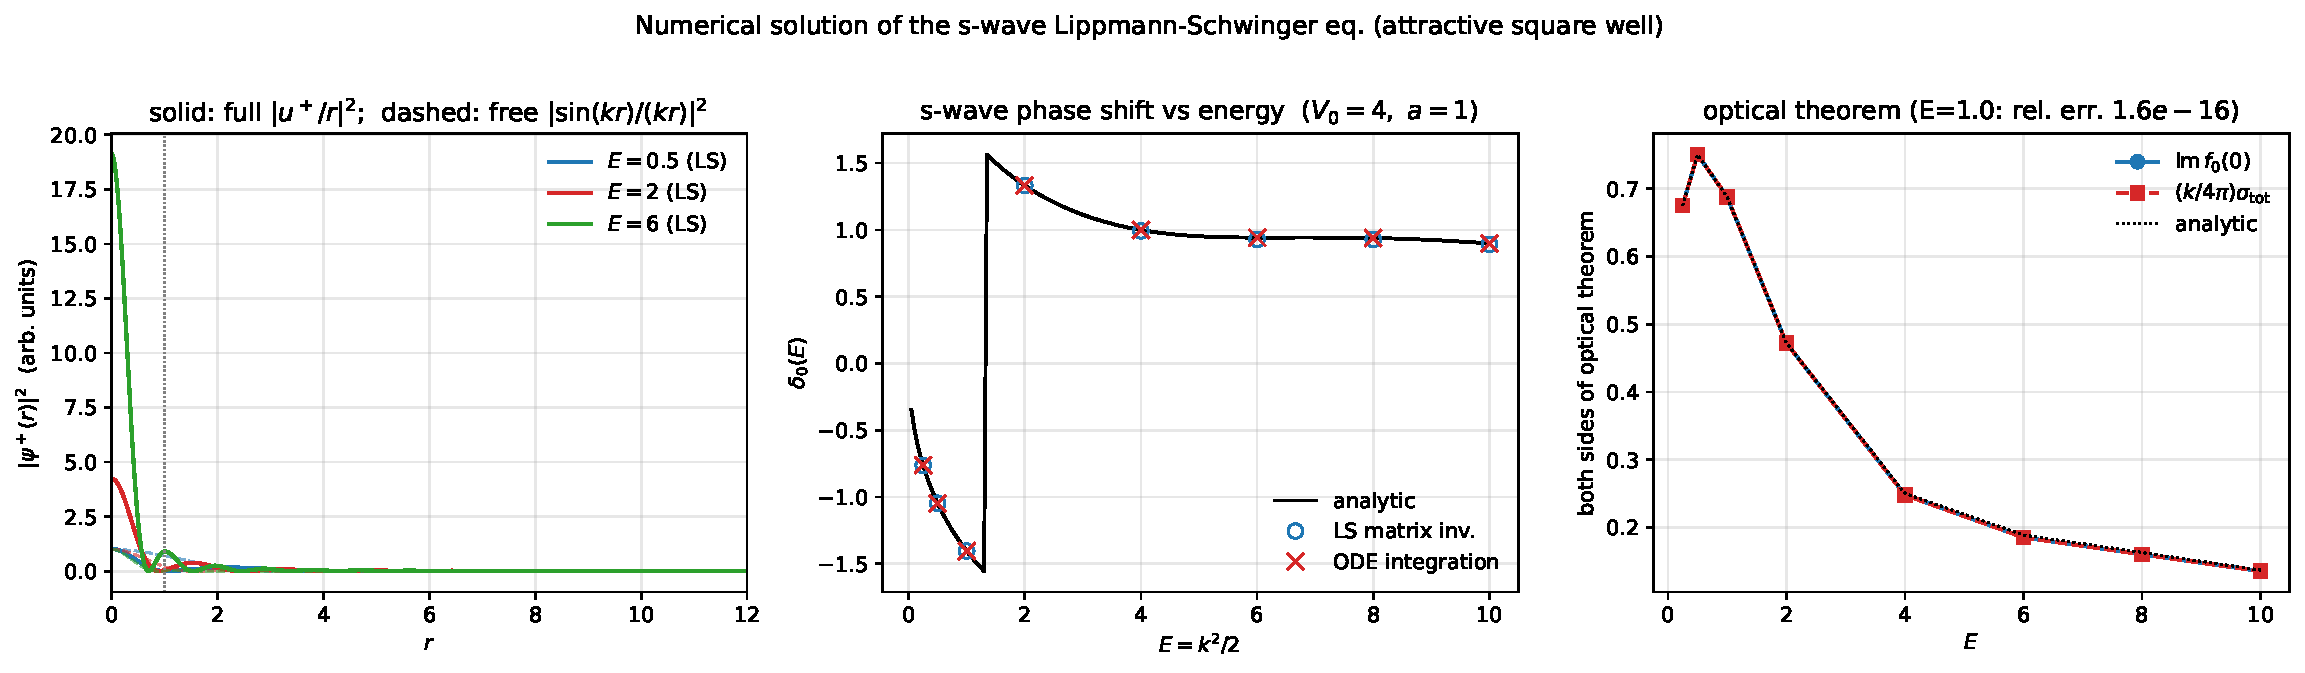
\includegraphics[width=0.98\linewidth]{ch09_lippmann_schwinger}
    \caption{s 波 LS 方程数值求解（吸引方势阱 $V_0=4,\,a=1$）。
      \textbf{左：}三个能量 $E=0.5, 2, 6$ 下 LS 矩阵反演的全解
      $|u^+(r)/r|^2$（实线）与无势自由解 $|\sin(kr)/(kr)|^2$（虚线）对比；
      在阱外（$r>a$，灰色虚线）两者频率相同但相位平移 $\delta_0$。
      \textbf{中：}两种方法提取的 $\delta_0(E)$（蓝圈、红叉）与解析公式
      （黑实线）逐点重合；约 $E\approx 1.5$ 处经过 $\delta_0 = \pi/2$（按
      Levinson 折叠至主值），表征第二个 s 波束缚态附近的能量阈，是低能共振
      行为的雏形。
      \textbf{右：}光学定理两端
      $\Im f_0(0) = \sin^2\delta_0/k$ 与 $(k/4\pi)\sigma_{\rm tot}^{\ell=0}
      = \sin^2\delta_0/k$（应严格相等，仅 s 波贡献），数值符合至机器精度
      ($\sim 10^{-16}$)。
    }\label{fig:numexp-ch09}
\end{figure}

\subsection*{物理讨论}
\begin{itemize}
\item \textbf{LS 与 ODE 的等价性.}\quad 图中两种方法的相移在
  $\sim 10^{-2}$ 级别一致；残余偏差来自 LS 离散化的中点积分误差，可通过细化
  $N$ 或换用 Simpson 权一致下降。这从数值上印证了 \eqref{eq:numex-LS-radial}
  与 Schrödinger 方程在适当边界条件下的等价性（Taylor §10.2）：积分方程把
  ``边界条件''——出射波/驻波——\emph{编码进 Green 函数选择}本身，从而
  ``一次性''给出物理解，而 ODE 方法须依赖 $r\to\infty$ 渐近匹配。
\item \textbf{$i\epsilon$ 处方与对称 Green 函数.}\quad 此处采用实数对称
  Green 函数（$K$ 矩阵语言），其 $r\to\infty$ 行为为驻波；要回到出射波振幅
  $f_0 = (e^{2i\delta_0}-1)/(2ik)$ 需通过 $\tan\delta_0 \leftrightarrow K$
  的代数关系（Taylor §10.4）。这避免了在数值上直接用 $i\epsilon$ 极限的
  Sokhotski 处方，是中心势计算的标准做法。
\item \textbf{光学定理的精确性.}\quad 因为单一 s 波下
  $f_0 = e^{i\delta_0}\sin\delta_0/k$，$\Im f_0(0)$ 与
  $(k/4\pi)\sigma_{\rm tot}^{\ell=0}$ 同为 $\sin^2\delta_0/k$，两者恒等
  ——这是\emph{相移参数化的内禀幺正性}的体现：$|S_0|=|e^{2i\delta_0}|=1$ 自动
  保证光学定理。这与上一节 Yukawa Born 近似的失败形成对照：\textbf{相移方
  法本身就是非微扰的、逐能量幺正的}，因而是定态散射数值实践的``正确轨道''。
\item \textbf{相移随能量的行为.}\quad 由 Levinson 定理，
  $\delta_0(0) - \delta_0(\infty) = n_b\pi$，其中 $n_b$ 是 s 波束缚态数；当前
  参数下 $\sqrt{2 V_0}\,a = 2\sqrt{2}\approx 2.83$，跨过 $\pi/2$ 一次，
  对应 $n_b = 1$ 个 s 波束缚态。图中 $\delta_0(E)$ 在低能段为负、随能量增加
  穿过主值边界后渐近趋零的整体行为与该计数一致。
\end{itemize}

\begin{remark}
本数值实验是后续第~\ref{ch:partial}~章``部分波法''的``零阶练手''：
所有解析与算法基础（径向 LS 方程、相移提取、单道光学定理）在此已具备；推广到
任意 $\ell$ 仅需把 $\sin(kr),\cos(kr)$ 替换为 Riccati--Bessel 函数
$\hat\jmath_\ell, \hat n_\ell$ 并修改有效势中的离心项，即 Taylor §11.2。
\end{remark}

\chapter{分波分析 (Partial Wave Analysis: Stationary)}\label{ch:partial}

对球对称势 $V(r)$ 的散射问题，角动量 $\Op{\mathbf L}^2$ 和 $\Op L_3$
均与 $\Op H$ 对易。因此 S 算子在 $\ket{E,l,m}$ 基底下是对角的。
按 $l$ 展开散射振幅，问题简化为一系列一维径向方程，每一分波
$l$ 由实参数相移 $\delta_l(p)$ 表征。本章按 Zhiguang 讲义 ch10
的结构系统讨论：分波 S 矩阵，自由径向波函数（Riccati--Bessel
族），分波散射态，分波 Lippmann--Schwinger 方程，分波振幅及其
低能行为，正则解与 Variable Phase 方法，正则波函数的迭代解，
Jost 函数的构造及其作为相移的解析延拓基石；附录给出常微分方程
Green 函数的推导。

\section{分波的 S 矩阵}\label{sec:pw-Smat}

考虑两无自旋粒子的散射，相互作用是球对称的。S 算子保持能量与角
动量（包括 $\Op{\mathbf L}^2$ 和 $\Op L_3$），故在 $\ket{E,l,m}$
基底下对角：
\begin{equation}\label{eq:Smatrix-elm}
\matel{E'\,l'\,m'}{\Smat}{E\,l\,m}
= \delta(E'-E)\,\delta_{ll'}\,\delta_{mm'}\,\mathbf{s}_l(p),
\qquad
\mathbf{s}_l(p)= \rme^{2\rmi\delta_l(p)}.
\end{equation}
$\delta_l(p)$ 称为第 $l$ 分波的相移 (phase shift)，幺正性
$|\mathbf{s}_l|=1$ 蕴含 $\delta_l\in\R$；$\delta_l$ 有 $n\pi$ 的
不确定性 ($n\in\Z$ modulo $\pi$)。

\subsection{分波振幅}

平面波 $\ket{\mathbf p}$ 可以用 $\ket{E,l,m}$ 展开：
\begin{equation}\label{eq:p-Elm}
\inn{\mathbf p}{E,l,m}= (mp)^{-1/2}\,\delta(E_p-E)\,Y_l^m(\hat{\mathbf p}).
\end{equation}
利用 $S$ 在该基的对角性，立刻得到散射振幅按勒让德多项式的展开：
\begin{align}\label{eq:f-PW}
f(\mathbf p'\leftarrow\mathbf p)
&= \sum_l (2l+1)\,f_l(p)\,P_l(\hat{\mathbf p}'\cdot\hat{\mathbf p}),\\
f_l(p) &= \frac{\mathbf s_l(p)-1}{2\rmi p}
       = \frac{\rme^{\rmi\delta_l(p)}\sin\delta_l(p)}{p},
\qquad \mathbf s_l(p)=\rme^{2\rmi\delta_l(p)}.\label{eq:fl-ch10}
\end{align}
$f_l(p)$ 称为分波振幅。它满足如下幺正圆 (unitarity circle)：
$pf_l$ 位于复平面上以 $\rmi/2$ 为圆心、半径为 $1/2$ 的圆上。

\subsection{分波截面}

由 $\rmd\sigma/\rmd\Omega = |f|^2$，在角积分时利用
$\int\rmd\Omega\,P_l P_{l'}=\frac{4\pi}{2l+1}\delta_{ll'}$，
得分波截面与总截面：
\begin{equation}\label{eq:sigma-l}
\sigma_l(p)
= 4\pi(2l+1)|f_l(p)|^2
= \frac{4\pi(2l+1)\sin^2\delta_l(p)}{p^2},
\qquad
\sigma=\sum_l\sigma_l(p).
\end{equation}

\begin{theorem}[幺正界 Unitary bound]\label{thm:unitary-bound}
对任意分波，
\begin{equation}
\sigma_l(p)\le \frac{4\pi(2l+1)}{p^2}.
\end{equation}
等号当且仅当 $\delta_l=\pi/2$ ($\bmod\pi$) 时取得。
\end{theorem}

\begin{remark}
光学定理在分波展开下的形式为
$\sigma=\frac{4\pi}{p}\Im f(0)
=\sum_l\frac{4\pi(2l+1)}{p}\Im f_l(p)
=\sum_l\frac{4\pi(2l+1)\sin^2\delta_l}{p^2}$，
两种写法一致。
\end{remark}

\section{自由的径向波函数}\label{sec:free-radial}

自由 Hamiltonian $H_0$ 在球坐标下，把 $\ket{E,l,m}$
表示成
$\inn{\mathbf x}{E,l,m}= \frac{y(r)}{r}\,Y_l^m(\hat{\mathbf x})$，
则约化径向方程为
\begin{equation}\label{eq:radial-free}
\Bigl[\frac{\rmd^2}{\rmd r^2}-\frac{l(l+1)}{r^2}+p^2\Bigr]y(r)=0,
\qquad p=(2mE)^{1/2}.
\end{equation}
两个独立解，分别在 $r\to 0$ 时趋于 $r^{l+1}$ 和 $r^{-l}$。物理
上可接受（在 $r\to0$ 趋于 $0$）的解为 Riccati--Bessel 函数：
\begin{equation}\label{eq:RBessel}
\hat\jmath_l(z)\equiv z\,j_l(z)
= \Bigl(\frac{\pi z}{2}\Bigr)^{1/2}J_{l+1/2}(z)
= z^{l+1}\sum_{n=0}^\infty \frac{(-z^2/2)^n}{n!\,(2l+2n+1)!!},
\end{equation}
其中 $j_l$ 是球贝塞尔函数。$\hat\jmath_l$ 在 $0$ 附近行为
$\hat\jmath_l\sim z^{l+1}/(2l+1)!!\,[1+O(z^2)]$，并有正交归一
$\int_0^\infty\rmd r\,\hat\jmath_l(p'r)\hat\jmath_l(pr)
=\frac{\pi}{2}\delta(p'-p)$。
归一化的自由径向波函数为
\begin{equation}\label{eq:free-Elm-x}
\inn{\mathbf x}{E,l,m}
= \rmi^l\Bigl(\frac{2m}{\pi p}\Bigr)^{1/2}
   \frac{1}{r}\,\hat\jmath_l(pr)\,Y_l^m(\hat{\mathbf x}).
\end{equation}

另一独立解（在 $r\to0$ 行为 $r^{-l}$）为 Riccati--Neumann 函数：
\begin{equation}\label{eq:RNeumann}
\hat n_l(z)\equiv z\,n_l(z)
= (-1)^l\Bigl(\frac{\pi z}{2}\Bigr)^{1/2}J_{-l-1/2}(z)
\sim z^{-l}(2l-1)!!\,[1+O(z^2)],\quad z\to 0.
\end{equation}

\subsection{Riccati--Hankel 函数与渐近行为}

$r\to\infty$ 时离心势项可忽略，方程退化为
$y''+p^2 y=0$；趋于 $\rme^{\pm\rmi pr}$ 的解为 Riccati--Hankel
函数：
\begin{equation}\label{eq:RHankel}
\hat h_l^\pm(z)\equiv \hat n_l(z)\pm\rmi\hat\jmath_l(z)
= \rme^{\pm\rmi(z-l\pi/2)}[1+O(z^{-1})].
\end{equation}
所以
\begin{align}
\hat\jmath_l(z) &= \frac{\hat h_l^+(z)-\hat h_l^-(z)}{2\rmi}
\xrightarrow{z\to\infty} \sin\!\Bigl(z-\tfrac{l\pi}{2}\Bigr),\label{eq:jhat-asy}\\
\hat n_l(z) &\xrightarrow{z\to\infty} \cos\!\Bigl(z-\tfrac{l\pi}{2}\Bigr).
\end{align}
低 $l$ 的具体形式：
\[
\begin{array}{c|ccc}
 & l=0 & l=1 & l=2\\\hline
\hat\jmath_l & \sin z & \frac{1}{z}\sin z-\cos z &
   \bigl(\frac{3}{z^2}-1\bigr)\sin z-\frac{3}{z}\cos z\\
\hat n_l & \cos z & \frac{1}{z}\cos z+\sin z &
   \bigl(\frac{3}{z^2}-1\bigr)\cos z+\frac{3}{z}\sin z\\
\hat h_l^+ & \rme^{\rmi z} & (1-\frac{1}{\rmi z})\rme^{\rmi(z-\pi/2)} &
   \bigl(1+\frac{3\rmi}{z}-\frac{3}{z^2}\bigr)\rme^{\rmi(z-\pi)}\\
\hat h_l^- & \rme^{-\rmi z} & (1+\frac{1}{\rmi z})\rme^{-\rmi(z-\pi/2)} &
   \bigl(1-\frac{3\rmi}{z}-\frac{3}{z^2}\bigr)\rme^{-\rmi(z-\pi)}
\end{array}
\]
反演与共轭关系：
\begin{equation}
\hat\jmath_l(-z)=(-)^{l+1}\hat\jmath_l(z),\quad
\hat n_l(-z)=(-)^l\hat n_l(z),\quad
\hat h_l^\pm(-z)=(-)^l\hat h_l^\mp(z),\quad
[\hat h_l^\pm(z)]^*=\hat h_l^\mp(z^*).
\end{equation}

\subsection{平面波的 Rayleigh 展开}

平面波用球面波展开（角动量基）：
\begin{align}
\ket{\mathbf p}
&= \int\rmd E\sum_{l,m}\ket{E,l,m}\inn{E,l,m}{\mathbf p}
= (mp)^{-1/2}\sum_{l,m}\ket{E_p,l,m}\,Y_l^m(\hat{\mathbf p})^*,\\
\inn{\mathbf x}{\mathbf p}
&= \Bigl(\frac{2}{\pi}\Bigr)^{1/2}\frac{1}{pr}
\sum_{l,m}\rmi^l\,\hat\jmath_l(pr)\,Y_l^m(\hat{\mathbf x})\,Y_l^m(\hat{\mathbf p})^*\\
&= (2\pi)^{-3/2}\frac{1}{pr}\sum_l (2l+1)\,\rmi^l\,
   \hat\jmath_l(pr)\,P_l(\hat{\mathbf x}\cdot\hat{\mathbf p}).
\label{eq:Rayleigh}
\end{align}
这就是 Rayleigh 公式。

\section{分波散射态}\label{sec:pw-states}

把自由球面波 $\ket{E,l,m}$ 通过 Mølller 算子映射，可以定义带相互
作用的散射态球面波 $\ket{E,l,m\pm}$：
\begin{equation}
\ket{E,l,m\pm}=\Op\Omega_\pm \ket{E,l,m},
\qquad
\inn{E',l',m'\pm}{E,l,m\pm}=\delta(E'-E)\delta_{l'l}\delta_{m'm}.
\end{equation}
由 $H\Omega_\pm=\Omega_\pm H_0$ 可知 $\ket{E,l,m\pm}$ 是 $\Op H$
的本征态：
\[ \Op H\ket{E,l,m\pm}=E\ket{E,l,m\pm}.\]
$\Op{\mathbf L}^2,\Op L_3$ 与 $\Op\Omega_\pm$ 对易，所以
$\ket{E,l,m\pm}$ 同时是 $\Op{\mathbf L}^2,\Op L_3$ 的本征态：
本征值仍为 $l(l+1),m$。可以认为 $\ket{E,l,m+}$ 是
$\ket{E,l,m}$ 在 $t=0$ 处对应的散射态。

\subsection{分波径向波函数 $\psi_{l,p}^{+}(r)$}

写
\begin{equation}\label{eq:Elm-plus-x}
\inn{\mathbf x}{E,l,m+}
= \rmi^l \Bigl(\frac{2m}{\pi p}\Bigr)^{1/2}\frac{1}{r}\,
   \psi_{l,p}^{+}(r)\,Y_l^m(\hat{\mathbf x}).
\end{equation}
当 $V=0$，$\psi_{l,p}^{+}(r)\to\hat\jmath_l(pr)$。归一化条件
$\inn{E',l',m'+}{E,l,m+}=\delta(E'-E)\delta_{l'l}\delta_{m'm}$
要求
\begin{equation}\label{eq:psi-norm}
\int_0^\infty \rmd r\,\psi_{l,p'}^{+\,*}(r)\,\psi_{l,p}^{+}(r)
=\frac{\pi}{2}\,\delta(p'-p).
\end{equation}
$\ket{\mathbf p+}$ 用 $\ket{E,l,m+}$ 展开后得到坐标空间形式：
\begin{equation}\label{eq:xpplus}
\inn{\mathbf x}{\mathbf p+}
= (2\pi)^{-3/2}\frac{1}{pr}\sum_l (2l+1)\,\rmi^l\,
\psi_{l,p}^{+}(r)\,P_l(\hat{\mathbf x}\cdot\hat{\mathbf p}).
\end{equation}
$\psi_{l,p}^{+}$ 满足径向薛定谔方程及边界条件
$\psi_{l,p}^{+}(0)=0$（以下省略上标 $+$）：
\begin{equation}\label{eq:radial-int}
\Bigl[\frac{\rmd^2}{\rmd r^2}-\frac{l(l+1)}{r^2}-U(r)+p^2\Bigr]
\psi_{l,p}(r)=0,\qquad U(r)\equiv 2m\,V(r).
\end{equation}

\subsection{渐近行为与相移}

$r\to\infty$ 时，由 \eqref{eq:xpplus} 与平面波加散射波渐近行为
$\inn{\mathbf x}{\mathbf p+}\sim
(2\pi)^{-3/2}[\rme^{\rmi\mathbf p\cdot\mathbf x}+f(p\hat{\mathbf x}\leftarrow\mathbf p)\rme^{\rmi pr}/r]$
对比，得
\begin{align}
\psi_{l,p}(r)
&\xrightarrow{r\to\infty} \hat\jmath_l(pr)
   + p\,f_l(p)\,\hat h_l^+(pr)\nonumber\\
&\xrightarrow{r\to\infty}
   \rme^{\rmi\delta_l(p)}\sin\!\Bigl[pr-\tfrac{l\pi}{2}+\delta_l(p)\Bigr].
\label{eq:psi-asy}
\end{align}
利用 $\hat\jmath=(\hat h^+ -\hat h^-)/(2\rmi)$ 并写成入射加出射波：
\begin{equation}\label{eq:psi-in-out}
\psi_{l,p}(r)\xrightarrow{r\to\infty}
\frac{\rmi}{2}\bigl[\hat h_l^-(pr)-\mathbf s_l(p)\,\hat h_l^+(pr)\bigr].
\end{equation}
第一项是入射球面波，第二项是散射后的出射球面波；幺正性
$|\mathbf s_l|=1$ 即“无粒子湮灭”，$\delta_l$ 是势造成的渐近正弦
波相位移动。

\begin{example}[方势阱与方势垒的物理图像]
对吸引势 $V(r)<0$，阱内动能比阱外大，相位变化更快，故 $V$ 把波函
数“向内拉”(pull inward)，给出正的相移；反之，排斥势 $V(r)>0$
则把波函数“向外推” (push outward)，给出负的相移。
\end{example}

\subsection{相移的积分表示}

比较两个势 $V(r),\hat V(r)$ 在同一能量下的相移
$\delta_l,\hat\delta_l$。相应径向方程
\begin{equation}
\Bigl[\frac{\rmd^2}{\rmd r^2}+\bigl(\epsilon-\tfrac{l(l+1)}{r^2}-U(r)\bigr)\Bigr]y_l=0,
\qquad
\Bigl[\frac{\rmd^2}{\rmd r^2}+\bigl(\epsilon-\tfrac{l(l+1)}{r^2}-\hat U(r)\bigr)\Bigr]\hat y_l=0,
\end{equation}
$r\to0$ 处 $y_l,\hat y_l\to0$；$r\to\infty$ 处
$y_l\sim\sin(pr-l\pi/2+\delta_l)$，$\hat y_l\sim\sin(pr-l\pi/2+\hat\delta_l)$。
Wronskian $W(y_l,\hat y_l)=y_l\hat y_l'-y_l'\hat y_l$ 在 $r=0$ 处为零，
$r\to\infty$ 时趋于 $p\sin(\delta_l-\hat\delta_l)$。利用恒等式
$W(y_l,\hat y_l)\big|_a^b=-\int_a^b\rmd r\,\hat y_l(U-\hat U)y_l$，取
$a\to0,b\to\infty$ 得
\begin{equation}\label{eq:phase-int}
\sin(\delta_l-\hat\delta_l)
= -\frac{2m}{\hbar^2 k}\int_0^\infty \rmd r\,\hat y_l(V-\hat V)\,y_l.
\end{equation}
取 $\hat V=0$（自由情形 $\hat\delta_l=0$），并要求 $V(r)$ 在
$r\to\infty$ 比 $1/r$ 更快地下降、$r\to0$ 处比 $1/r^2$ 弱发散：
\begin{equation}\label{eq:phase-int2}
\sin\delta_l=-\frac{2m}{\hbar^2 k}\int_0^\infty \rmd r\,\hat\jmath_l(kr)\,V(r)\,y_l(r)\,r\,.
\end{equation}
(等价的另一形式 $\sin\delta_l=-\frac{2m}{\hbar^2k}\int_0^\infty\hat\jmath_l\,V\,y_l\,\rmd r$.)
当 $\Delta V$ 极小（一阶微扰）时
$\Delta\delta_l = -\frac{2m}{\hbar^2k}\int_0^\infty(V-\hat V)y_l^2\,\rmd r$，
势变浅（更吸引）相移变大；势变深（更排斥）相移变小。

\section{分波 Lippmann--Schwinger 方程及分波振幅}\label{sec:pw-LS}

把 LS 方程 $\ket{\mathbf p\pm}=\ket{\mathbf p}+G_0(E_p\pm\rmi\epsilon)V\ket{\mathbf p\pm}$
投影到 $\ket{E,l,m}$ 基底，得
\[
\ket{E_p,l,m\pm}=\ket{E_p,l,m}+G_0(E_p\pm\rmi\epsilon)V\ket{E_p,l,m\pm}.
\]
写在坐标表象，并把自由 Green 函数按角动量分解，可得分波形式的
LS 方程。

\subsection{自由分波 Green 函数}

把自由 Green 函数 $G_0(z)$ 按 $\ket{E,l,m}$ 分解：
\begin{equation}
\matel{\mathbf x}{G_0(z)}{\mathbf x'}
= -\Bigl(\frac{2m}{prr'}\Bigr)\sum_{lm}
   Y_l^m(\hat{\mathbf x})Y_l^{m*}(\hat{\mathbf x'})\,
   \hat h_l^+(pr_>)\,\hat\jmath_l(pr_<),\quad
p=\sqrt{2mz}.
\end{equation}
定义 $r_>=\max(r,r')$，$r_<=\min(r,r')$，则分波 Green 函数为
\begin{equation}\label{eq:G0lp}
G_{l,p}^{0}(r,r')= -\frac{\hat h_l^+(pr_>)\,\hat\jmath_l(pr_<)}{p}.
\end{equation}

\subsection{分波 LS 方程}

定义 $U(r)=2mV(r)$，则
\begin{align}\label{eq:LS-pw}
\psi_{l,p}^{+}(r)
&= \hat\jmath_l(pr) - \frac{1}{p}\int_0^\infty \rmd r'\,
   \hat h_l^+(pr_>)\,\hat\jmath_l(pr_<)\,U(r')\,\psi_{l,p}^{+}(r')\nonumber\\
&= \hat\jmath_l(pr)+\int_0^\infty \rmd r'\,
   G_{l,p}^{0}(r,r')\,U(r')\,\psi_{l,p}^{+}(r').
\end{align}
算子形式可以简写为
\begin{equation}\label{eq:LS-op}
\psi_{l,p}=\hat\jmath_l+G_{l,p}^{0}\,U\,\psi_{l,p},
\end{equation}
其迭代级数解（玻恩级数的分波形式）为
\[
\psi_{l,p}=\hat\jmath_l+G_{l,p}^{0}U\hat\jmath_l+(G_{l,p}^{0}U)^2\hat\jmath_l+\cdots
\]

\subsection{分波振幅的积分公式}

由 $f(\mathbf p'\leftarrow\mathbf p)=-(2\pi)^2 m\matel{\mathbf p'}{V}{\mathbf p+}$
出发并代入 \eqref{eq:xpplus}，比较 $P_l$ 系数：
\begin{align}
f(\mathbf p'\leftarrow\mathbf p)
&= -(8\pi)\frac{m}{p^2}\int\rmd r\sum_{l,m}
   Y_l^m(\hat{\mathbf p}')Y_l^{m*}(\hat{\mathbf p})\,
   \hat\jmath_l(p'r)\,\psi_{l,p}^{+}(r)\,V(r)\nonumber\\
&= -\frac{1}{p^2}\sum_l (2l+1)\,P_l(\hat{\mathbf p}\cdot\hat{\mathbf p}')
   \int\rmd r\,\hat\jmath_l(p'r)\,\psi_{l,p}^{+}(r)\,U(r),
\end{align}
得到
\begin{equation}\label{eq:fl-ch10-int}
\boxed{\;f_l(p)=-\frac{1}{p^2}\int_0^\infty \rmd r\,
   \hat\jmath_l(pr)\,\psi_{l,p}^{+}(r)\,U(r)\;}
\end{equation}
代入 $\psi_{l,p}$ 的迭代级数即得 $f_l(p)$ 的玻恩级数：
\begin{equation}
f_l(p)=-\frac{1}{p^2}\Bigl(\int_0^\infty \rmd r\,\hat\jmath_l\,U\,\hat\jmath_l
+\int_0^\infty \rmd r\,\hat\jmath_l\,U\,G_{l,p}^{0}\,U\,\hat\jmath_l+\cdots\Bigr).
\end{equation}

\subsection{Born 近似的相位结构}

最低阶 (Born approximation)
\begin{equation}\label{eq:fl-ch10-Born}
f_l^{\rm B}(p)=-\frac{1}{p^2}\int_0^\infty \rmd r\,\hat\jmath_l(pr)^2\,U(r),
\end{equation}
即 $s$ 波 ($\hat\jmath_0=\sin z$)
\[
f_0^{\rm B}(p)=-\frac{1}{p^2}\int_0^\infty \rmd r\,\sin(pr)\,U(r)\,\sin(pr).
\]
\textbf{说明：}玻恩近似的振幅是\emph{实}的；而严格的振幅
$f_l(p)=p^{-1}\rme^{\rmi\delta_l}\sin\delta_l$ 是\emph{复}的，
位于幺正圆上。仅当 $\delta_l\,(\bmod\pi)$ 很小时玻恩近似才合理。
图示上，幺正圆为以 $\rmi/2$ 为心、半径 $1/2$ 的圆，玻恩近似只
保留圆在原点处的切线方向。

\section{分波振幅的性质}\label{sec:pw-properties}

\subsection{对势的假设}

引入参数 $\lambda$，把方程写为
\begin{equation}\label{eq:radial-lambda}
\Bigl[\frac{\rmd^2}{\rmd r^2}-\frac{l(l+1)}{r^2}+p^2-\lambda U(r)\Bigr]\psi_{l,p}(r)=0.
\end{equation}
为后面的解析性分析，假设 $V(r)$ 满足
\begin{itemize}
\item $r\to\infty$，$V(r)=O(r^{-3-\epsilon})$，$\epsilon>0$；
（实际多数情形只要 $V(r)=O(r^{-2-\epsilon})$ 即可）
\item $r\to 0$，$V(r)=O(r^{-3/2-\epsilon})$；（有时仅
  $V(r)=O(r^{-2+\epsilon})$ 即足够）
\item $V(r)$ 除有限点处的有限跳跃外在 $0<r<\infty$ 上连续。
\end{itemize}

\subsection{弱势/高能极限}

若 $\lambda U(r)\ll |l(l+1)/r^2-p^2|$，方程近似为自由径向方程：
$\psi_{l,p}\to\hat\jmath_l(pr)$，从而 $pf_l(p)\sim\rme^{\rmi\delta_l}\sin\delta_l\to0$，
故 $\delta_l\to n\pi$ ($n\in\Z$ modulo $\pi$ 不确定)。具体地：
\begin{itemize}
\item $\lambda\to0$ (弱势)：$f_l\to0$，$\delta_l\to n\pi$；
\item 给定 $l$, $E\to\infty$：$pf_l\to0$，$\delta_l\to n\pi$；
\item $p\to\infty$，规定 $\delta_l\to0$（消除 $n\pi$ 不确定性），则
  $\lambda\to0$ 时也有 $\delta_l\to 0$；
\item 给定势与能量，$l\to\infty$：离心势 $l(l+1)/2mr^2$ 越来越强，
  粒子穿入势的深度越来越小，相互作用变弱，相移变小。
\end{itemize}
经典图像可估出明显相移所对应的 $l_{\max}\sim pa$（$a$ 为势作用
半径）。当 $l\gg pa$ 时，玻恩近似对该分波都很好。

\subsection{分波波函数与振幅的低能行为}

考虑 \eqref{eq:LS-pw}。$p\to0$ 时 Green 函数的极限为
\begin{equation}
G_{l,p}^{0}(r,r')\xrightarrow{p\to 0}
-\frac{(r_<)^{l+1}\,(r_>)^{-l}}{2l+1},
\end{equation}
与 $p$ 无关。由 LS 方程，$\psi_{l,p}(r)$ 在 $p\to0$ 时与
$\hat\jmath_l(pr)\propto p^{l+1}r^{l+1}$ 同阶：
\begin{equation}
\psi_{l,p}(r)\xrightarrow{p\to 0} p^{l+1}\times(\text{$p$ 无关函数}).
\end{equation}
代入 \eqref{eq:fl-ch10-int} 得
\begin{equation}\label{eq:fl-ch10-low}
f_l(p)\xrightarrow{p\to 0} -a_l\,p^{2l},\qquad
\rme^{\rmi\delta_l(p)}\sin\delta_l(p)\to -a_l\,p^{2l+1}.
\end{equation}
$a_l$ 称为散射长度 (scattering length)，仅在 $l=0$ 时具有长度
量纲（$a_0$）。
\begin{itemize}
\item 若势在 $r>a$ 时 $U=0$：上述结论严格成立。
\item 若 $V(r)$ 比 $1/r^n$ 任意 $n$ 都更快下降，结论亦成立。
\item 若 $V(r)\sim 1/r^\nu$，仅在 $l\ge(\nu-3)/2$ 时成立。
\item 后面会看到某些条件下 $a_l\to\infty$ (零能共振、束缚态阈值)。
\end{itemize}
\begin{remark}
有些文献把散射长度定义差一个符号 $f_l\to a_l p^{2l}$。一般来说
仅把 $l=0$ 的 $a_0$ 称为散射长度。
\end{remark}

\subsection{$p\to0$ 时的物理含义}

假设 \eqref{eq:fl-ch10-low} 成立：
\begin{itemize}
\item $l=0$（$s$ 波）: $f_0\to -a_0\ne 0$。
\item $l\ne 0$: $f_l\to 0$。
\item 总振幅 $f(\mathbf p'\leftarrow\mathbf p)=\sum_l(2l+1)f_l P_l(\cos\theta)\to -a_0$，
  与角度无关。
\item $\lim_{p\to0}\rmd\sigma/\rmd\Omega = a_0^2$，
  $\sigma_{\rm tot}\to 4\pi a_0^2$。
\item $f_l=p^{-1}\rme^{\rmi\delta_l}\sin\delta_l\sim -a_l p^{2l}$，
  即 $\delta_l\to n\pi-a_l p^{2l+1}$；$a_l\in\R$。
\item 若约定 $p\to\infty$ 时 $\delta_l\to0$，则 $\delta_l$ 没有
  $n\pi$ 不确定性，但 $p\to0$ 时 $\delta_l$ 不一定趋于 $0$。
\end{itemize}

\begin{theorem}[Levinson 定理（预告）]\label{thm:Levinson}
满足上述条件的 $V(r)$，
\begin{equation}
\delta_l(0)-\delta_l(\infty) = n_l\,\pi,
\end{equation}
$n_l$ 是角动量为 $l$ 的束缚态的个数。约定 $\delta_l(\infty)=0$，
则 $\delta_l(0)=n_l\pi$。一个例外：$s$ 波散射长度 $a_0=\infty$
（零能阈共振）时，$\delta_0(0)=(n_0+\tfrac12)\pi$。
\end{theorem}

\subsection{方阱例 (作业)}

球方阱 $V(r)=-V_0\,(r<a),\,0\,(r>a)$，取
$(2ma^2 V_0)^{1/2}=4.8$。可证此时 $l=0$ 有两个束缚态，
$l=1,2$ 各一个束缚态。验证：
\begin{enumerate}
\item $\delta_0(0)=2\pi,\delta_1(0)=\delta_2(0)=\pi$，其它分波
  $\delta_l(0)=0$；分波散射截面
  $\sigma_l(0)\approx 45\pi a^2$，$\sigma_{l>0}(0)=0$；
\item $l$ 增大、$p\to 0$ 时 $\delta_l\to n\pi-a_l p^{2l+1}$，
  越来越平缓；
\item $0\le pa\lesssim 1$ 时 $\sigma_0$ 给出 90\% 截面贡献；
  $1\le pa\lesssim 2$ 时 $\sigma_0+\sigma_1+\sigma_2$ 主导；
\item 在 $pa=10$ 时所有相移小于 $60^\circ$，$pa=50$ 时小于
  $15^\circ$；
\item $pa=2.7$ 时 $s$ 波相移为 $\pi$，$\sigma_0=0$。势阱内波函
  数恰好比自由情形多了一个完整周期，出势阱后跟自由波函数无区别。
  当此现象发生时所有 $l>0$ 截面也可忽略，且发生在低能，则称
  \emph{Ramsauer--Townsend 效应}；
\item 在 $pa=2.6$、$l=3$ 处相移最快通过 $\pi/2$，$\sigma_3$ 有
  尖锐峰，是\emph{共振}现象——势几乎能束缚住 $l=3$ 态但还没
  完全束缚住。
\end{enumerate}

%======================================================================
\section{散射长度与有效程展开 (Scattering Length and Effective Range)}\label{sec:eff-range-main}

低能 ($pa\ll 1$) 散射的两个最重要参数是\textbf{散射长度} $a_0$ 与\textbf{有效程} $r_0$. 它们抓住了"势的细节怎么进入低能可观测量"的全部首阶信息——只要势是\emph{短程的} (有限程或指数衰减), 任何低能截面都只通过 $a_0,r_0$ 进入. 这一节把第 \S\ref{sec:Jost-low} 节出现的散射长度概念、第 \S\ref{sec:pw-eff-range} 节的 Bethe 公式证明, 与第~\ref{ch:analytic}~章 \S\ref{ssec:effective-range} 节由解析性导出的有效程展开\textbf{统一}到一个独立的节里, 并强调若干物理图像与现代应用 (halo, BEC, Wigner 阈值定律).

\subsection{散射长度: 定义与几何意义}\label{sec:eff-range-a0}

设势是\emph{有限程}的: $V(r)=0$ ($r>R$). 在 $r>R$ 区域 $s$ 波约化波函数是\emph{自由}的:
\begin{equation}
  u_0(r)\equiv r\psi_0(r)\xrightarrow{r>R}\frac{1}{p}\sin\bigl[pr+\delta_0(p)\bigr],
  \label{eq:eff-u-outside}
\end{equation}
取 $p\to 0$ 极限:
\begin{equation}
  u_0(r)\xrightarrow{p\to 0}r+\frac{\delta_0(p)}{p}=r-a_0,\qquad
  \boxed{\;a_0\equiv -\lim_{p\to 0}\frac{\delta_0(p)}{p}.\;}
  \label{eq:eff-a0-def}
\end{equation}

\paragraph{几何图像.}\quad $u_0(r)$ 在 $r>R$ 是一条直线 (零能下 $u_0''=0$). $a_0$ 是这条直线\emph{延拓回去与 $r$ 轴的截距}:
\[
  u_0(r)=r-a_0\implies u_0(a_0)=0,
\]
即零能下 $u_0$ 的"虚拟零点"在 $r=a_0$.

\begin{itemize}
  \item $a_0>0$: 零点在 $r$ 轴正方向, \emph{排斥型}或弱吸引势 (波函数被推出去).
  \item $a_0<0$: 零点在 $r$ 轴负方向 (即外推线穿过原点左侧), \emph{吸引}但尚未束缚的势.
  \item $a_0=\pm\infty$: 直线水平, 出现\emph{零能共振} (即将束缚的阈值情形).
\end{itemize}

\subsection{有效程: 定义与几何意义}\label{sec:eff-range-r0}

低能展开式 (Bethe 1949):
\begin{empheq}[box=\fbox]{equation}
  p\cot\delta_0(p)=-\frac{1}{a_0}+\frac{1}{2}r_0\,p^2+v_0\,p^4+\cdots,
  \label{eq:eff-bethe}
\end{empheq}
其中 $r_0$ 称\textbf{有效程} (effective range), $v_0$ 称\textbf{shape parameter}. \eqref{eq:eff-bethe} 由势的解析性给出 (有限程或指数衰减), 在 $p^2$ 解析意义下展开 (证明见 \S\ref{sec:pw-eff-range} 与 \S\ref{ssec:effective-range}).

\paragraph{$r_0$ 的几何含义.}\quad 把零能 $u_0(r)=r-a_0$ 与有限能 $\bar u_0(r;p)\equiv\sin[pr+\delta_0(p)]/p\cos\delta_0(p)$ 比较 (后者归一化使 $\bar u_0(0)\to-a_0$ 与零能解一致). 有效程的紧凑表示 \eqref{eq:pw-r0}:
\begin{equation}
  r_0=2\int_0^\infty\rmd r\,\bigl[\bar\phi_{0,0}(r)^2-\phi_{0,0}(r)^2\bigr],
  \label{eq:eff-r0-formula}
\end{equation}
其中 $\bar\phi_{0,0}(r)=r-a_0$ 是\emph{自由}零能解 (取与势作用区域一致的外延), $\phi_{0,0}(r)$ 是\emph{物理}零能解 (受势影响, 内区由 $V$ 决定, 外区按 $r-a_0$ 渐近). 故 \eqref{eq:eff-r0-formula} 度量"势对零能波函数的扰动"在 $L^2$ 意义下的强度.

\paragraph{粗略尺度.}\quad 对吸引短程势, 通常 $r_0\sim R$ ($R$ 为势的有效程, 故得名). 在自然单位 ($\hbar=1$, 长度量纲) 下 $r_0$ 是长度. $r_0>0$ 几乎总是成立 (除非势"特殊设计"使 $\phi_{0,0}^2>\bar\phi_{0,0}^2$, 实际情形罕见).

\subsection{$l$ 阶推广}\label{sec:eff-range-l}

对一般分波 $l\ge 0$, 在 \S\ref{sec:pw-eff-range} 中证明
\begin{equation}
  p^{2l+1}\cot\delta_l(p)=-\frac{1}{a_l}+\frac{1}{2}r_l\,p^2+v_l\,p^4+\cdots,
  \label{eq:eff-bethe-l}
\end{equation}
$a_l$ 是\emph{$l$ 阶散射长度} (量纲 $[L]^{2l+1}$, 注意只有 $l=0$ 是真正的长度), $r_l$ 是 $l$ 阶有效程. 高 $l$ 实验上很难独立测量, 主要由\emph{短程势}背景决定且小 (有效势 $l(l+1)/r^2$ 在低能压制了高分波贡献), 但在精密拟合 ($NN$ 散射, 冷原子) 中 $p$ 波散射长度 $a_1$ 也是相关物理量.

\subsection{Wigner 阈值定律 (Wigner threshold law)}\label{sec:eff-range-Wigner}

直接由 \eqref{eq:eff-bethe-l} 推出: 在 $p\to 0$ 时
\begin{equation}
  \delta_l(p)\xrightarrow{p\to 0}-a_l\,p^{2l+1},\qquad
  \sin^2\delta_l\sim a_l^2 p^{4l+2},
\end{equation}
\begin{empheq}[box=\fbox]{equation}
  \sigma_l(p)=\frac{4\pi(2l+1)}{p^2}\sin^2\delta_l\xrightarrow{p\to 0}4\pi(2l+1)a_l^2\,p^{4l}.
  \label{eq:eff-Wigner-law}
\end{empheq}
这就是\textbf{Wigner 阈值定律}: $l$ 波截面以 $p^{4l}$ 阈值幂律趋近其零能极限.
\begin{itemize}
  \item $l=0$: $\sigma_0\to 4\pi a_0^2$ 是\emph{有限}的——$s$ 波低能截面饱和, 称\emph{Wigner 阈值常数}. 量子力学最具反常的低能结果之一.
  \item $l\ge 1$: $\sigma_l\to 0$ 以 $p^{4l}$ 幂律. 故\emph{低能下只剩 $s$ 波}.
\end{itemize}
注意 \eqref{eq:eff-Wigner-law} 仅在\emph{短程势} (指数衰减或快于 $1/r^{2l+3}$) 下成立; 长程势 $1/r^\nu$ 在 $l$ 与 $\nu$ 不匹配时\emph{破坏} Wigner 律, 见 \S\ref{sec:eff-range-long-range}.

\subsection{ANC 与束缚态的低能关联}\label{sec:eff-range-ANC}

若势存在一个 $s$ 波束缚态, 衰减率 $\kappa$, 渐近波函数
$\phi_n(r)\xrightarrow{r\to\infty}c\rme^{-\kappa r}$, \emph{ANC (asymptotic normalization constant)} $c$ 与 $a_0,r_0$ 满足显式关系: 由 Jost 函数 $f_0(p)$ 在 $p=\rmi\kappa$ 处的零点条件展开
\begin{equation}
  f_0(\rmi\kappa)=0\implies p\cot\delta_0(p)\Big|_{p=\rmi\kappa}=-\kappa,
\end{equation}
代入 \eqref{eq:eff-bethe}:
\begin{equation}
  -\kappa=-\frac{1}{a_0}-\frac{1}{2}r_0\,\kappa^2,
\end{equation}
解出
\begin{equation}
  \boxed{\;\kappa=\frac{1}{r_0}\Bigl(1-\sqrt{1-\frac{2 r_0}{a_0}}\,\Bigr)
  \xrightarrow{r_0/a_0\ll 1}\frac{1}{a_0}+\frac{r_0}{2a_0^2}+\cdots\;}
  \label{eq:eff-kappa-from-a0-r0}
\end{equation}
对\emph{halo 系统} ($a_0\gg r_0$, 即非常弱束缚态): $\kappa\approx 1/a_0$, 束缚态半径 $\sim a_0$, 远远大于势的真实程. 这是\textbf{halo 核} (例 $^{11}$Be, $^{6}$He) 与\textbf{Efimov 物理}的核心.

ANC $c$ 与有效程的关系:
\begin{equation}
  c^2=\frac{2\kappa}{1-\kappa r_0}.
  \label{eq:eff-ANC-r0}
\end{equation}
故由测量 $a_0,r_0$ 即可推算近阈束缚态的能量 + ANC. 这是低能核物理\emph{universal relations} 的范式.

\subsection{零能共振与束缚态阈值}\label{sec:eff-range-zero}

考虑势随耦合常数 $\lambda$ 变深的过程: $V=\lambda V_0$. 当 $\lambda$ 增加, 第 $n$ 个束缚态从连续谱中冒出. 在阈值附近:
\begin{itemize}
  \item $\lambda$ 略小于阈值 $\lambda_n^*$: 没有第 $n$ 个束缚态, 但相空间已被它"准备好". 由 \eqref{eq:eff-kappa-from-a0-r0}, $a_0\to-\infty$, $\sigma_0\to\infty$ (零能共振).
  \item $\lambda=\lambda_n^*$: 阈值, $a_0=\pm\infty$, 严格的\emph{$0$ 能束缚态}出现 ($\kappa=0$).
  \item $\lambda$ 略大于 $\lambda_n^*$: 束缚态出现, $\kappa$ 从零开始增长, $a_0\to+\infty$ 然后逐渐减小到 $O(R)$.
\end{itemize}
即 $a_0$ 作为 $\lambda$ 的函数, 在每个束缚态阈值 $\lambda_n^*$ 处经历\textbf{$-\infty\to+\infty$ 的跳变}. 这就是 \S\ref{sec:pw-Levinson} 例外条款 $\delta_0(0)=(n_0+\tfrac12)\pi$ 在物理上的表现, 也是 Feshbach 共振 (磁场调节 $\lambda\propto B-B_0$) 的本质机制.

\subsection{长程势的修正展开}\label{sec:eff-range-long-range}

\eqref{eq:eff-bethe} 假设势短程 (指数衰减). 对\emph{长程} $V(r)\sim -C_\nu/r^\nu$ 势 ($r\to\infty$):
\begin{itemize}
  \item $\nu>2l+3$: 仍可写整数幂展开, 但 $r_l$ 可能依赖 $C_\nu$.
  \item $\nu=2l+3$: \emph{边界情形}, 出现对数. 例如 $\nu=3, l=0$: $V\sim -C_3/r^3$ 给 $p\cot\delta_0=-1/a_0+(2 C_3/3)\ln(pR_0)+O(p^2)$.
  \item $\nu<2l+3$: 整数幂展开\emph{失败}, 改用\textbf{modified effective range expansion} (Mott-Massey, O'Malley 1961):
    \begin{equation}
      \frac{p^{2l+1}\cot\delta_l}{M_l(p)}=-\frac{1}{a_l^{\rm M}}+\frac{1}{2}r_l^{\rm M}p^2+\cdots,
    \end{equation}
    $M_l(p)$ 是与长程势相关的修正函数 (Coulomb, $1/r^4$ 极化势等都有自己的 $M_l$).
\end{itemize}
\textbf{冷原子物理}中典型情形 $V\sim -C_6/r^6$ (van der Waals): $l=0$ 仍可整数幂展开但 $r_0$ 公式含 $C_6$ 修正 (Gribakin--Flambaum 1993).

\textbf{Coulomb}修正下 (见 \S\ref{sec:coulomb-plus-shortrange}): $p\cot\delta_0$ 替换为
\begin{equation}
  C_0^2(\eta)\bigl[p\cot\delta_0-2\eta p h(\eta)\bigr]=-1/a_C+\tfrac{1}{2}r_C p^2+\cdots,
\end{equation}
$C_0(\eta)$ 是 Coulomb 阻尼因子, $h(\eta)$ 是 digamma 修正——\emph{Coulomb 修正的有效程展开}, 适用于 $pp$, $\alpha\alpha$ 低能散射.

\subsection{现代应用速览}\label{sec:eff-range-modern}

\begin{itemize}
  \item \textbf{核物理}: $np$ 单态 $a_0^{(s)}=-23.7\,{\rm fm}$, $r_0^{(s)}=2.7\,{\rm fm}$; $np$ 三态 $a_0^{(t)}=5.4\,{\rm fm}$, 给氘的 ANC 与束缚能.
  \item \textbf{冷原子 BEC}: $^{87}$Rb 自旋极化态 $a_0\approx 100 a_{\rm Bohr}$. 通过 Feshbach 共振调谐 $a_0(B)$ 可从弱排斥到强吸引连续过渡 (BCS-BEC crossover).
  \item \textbf{Halo 核}: $^{11}$Be 单中子 halo, $\kappa\approx 0.16\,{\rm fm}^{-1}$, $1/a_0\approx 0.14\,{\rm fm}^{-1}$, 满足 \eqref{eq:eff-kappa-from-a0-r0} 的 universality.
  \item \textbf{Efimov 物理}: 三玻色子系统在 $a_0\to\pm\infty$ 阈值附近出现指数堆积束缚态 ($E_n=E_0\rme^{-2\pi n/s_0}$, $s_0\approx 1.00624$ 普适常数). 这是 $a_0$ 调控低能普适性的极端体现.
  \item \textbf{量子模拟}: 把冷原子做的有效低能哈密顿量映射回核物理 $NN$ 系统, 通过 $a_0$ 实现"\textbf{universality at unitarity}".
\end{itemize}

\subsection{与本章其他工具的接口}\label{sec:eff-range-interface}

\begin{itemize}
  \item 与 \S\ref{sec:Jost} \textbf{Jost 函数}: $a_l=-\Re f_l(0)$ 的\emph{零阶系数}, $r_l$ 由 $f_l$ 在 $p=0$ 邻域的二阶导数决定. 见 \S\ref{sec:pw-eff-range} 完整证明.
  \item 与 \S\ref{sec:Rmatrix} \textbf{R-矩阵}: 单极 R-矩阵参数化 $\gamma^2/(E_1-E)$ 给低能 $K$-matrix, 可\emph{直接读出} $a_0, r_0$ 与 $\gamma, E_1$ 的关系——这是核物理 R-matrix code 直接输出 $a_0, r_0$ 的算法基础.
  \item 与 \S\ref{ssec:effective-range} \textbf{解析性}: $p\cot\delta_0$ 关于 $p^2$ 在原点的解析性是 \eqref{eq:eff-bethe} 存在的\emph{必要条件}; 长程势破坏解析性即破坏展开 (\S\ref{sec:eff-range-long-range}).
\end{itemize}

\section{正则解 (Regular solution) 及 Variable Phase Method}\label{sec:regular}

\subsection{正则解 $\phi_{l,p}(r)$}

考虑径向方程 \eqref{eq:radial-int}。归一化的 $\psi_{l,p}(r)$ 满足
\eqref{eq:psi-norm}，边界条件
$\psi_{l,p}(0)=0$；$r\to\infty$ 时
$\psi_{l,p}\to\hat\jmath_l(pr)+pf_l\hat h_l^+(pr)$。
现在定义另一个解 $\phi_{l,p}(r)\propto \psi_{l,p}(r)$，仅归一化
不同。其边条件定义在一点 $r\to0$，包括值与导数：
\begin{equation}\label{eq:phi-bc}
\phi_{l,p}(r)\xrightarrow{r\to 0}\hat\jmath_l(pr).
\end{equation}
显然，$\phi_{l,p}(r)$ 是\emph{实}的（边界条件实，方程实）。

\subsection{Variable Phase 方法}

为简洁起见仅考虑 $s$ 波。引入截断势
\begin{equation}
V_\rho(r)=\begin{cases} V(r), & r\le \rho,\\ 0,& r>\rho.\end{cases}
\end{equation}
势 $V(r)$ 的 $s$ 波正则解记为 $\phi(r)$、相移 $\delta$；
$V_\rho(r)$ 对应记为 $\phi_\rho(r),\delta(\rho)$。
\begin{itemize}
\item $\rho=0$：无势，约定 $\delta(0)=0$；
\item $\lim_{\rho\to\infty}\delta(\rho)=\delta$；
\item $\forall\rho$，$\phi$ 与 $\phi_\rho$ 在 $r=0$ 有同样边条件、
  且在 $0\le r\le\rho$ 满足同一方程，因此
  $\phi(r)=\phi_\rho(r),\;0\le r\le\rho$；
\item $r>\rho$，$\phi_\rho(r)$ 满足自由 ($l=0$) 径向方程，故为
  正弦形式：$\phi_\rho(r)=\alpha(\rho)\sin[pr+\delta(\rho)]$。
\end{itemize}
由 $\phi$ 在 $\rho$ 处与 $\phi'$ 处的连续性
\begin{align}
\phi(\rho)&=\alpha(\rho)\sin[p\rho+\delta(\rho)],\\
\phi'(\rho)&=p\alpha(\rho)\cos[p\rho+\delta(\rho)].
\end{align}
上两式对任意 $r=\rho$ 都成立，可把所有 $\rho$ 换成 $r$；带入定态径向
方程 $[d^2/dr^2+p^2-U(r)]\phi=0$ 消掉 $\alpha$ 得到 \emph{$s$ 波相移
方程}：
\begin{equation}\label{eq:variable-phase}
\boxed{\;\delta'(r)=-\frac{1}{p}\,U(r)\,\sin^2[pr+\delta(r)].\;}
\end{equation}
（作业：补全推导。）

\subsection{相移方程的物理含义}

由 \eqref{eq:variable-phase}：
\begin{itemize}
\item 右边的符号只取决于 $U(r)$ 的符号：吸引势 $V\le0$ 给出
  正相移；排斥势 $V\ge0$ 给出负相移。
\item 若 $V_1(r)\ge V_2(r)$ 对所有 $r$，则 $\delta_1\le\delta_2$。
\item 替换 $V\to\lambda V$，则
  $\delta=-\frac{\lambda}{p}\int_0^\infty\rmd r\,U(r)\sin^2[pr+\delta(r)]$。
  设 $V(r)\sim 1/r^{1-\epsilon}$（$r\to0$），则
  $|\delta|\le|\lambda/p|\int_0^\infty\rmd r|U(r)|$，故
  $\delta\to0$ 当 $\lambda\to0$ 或 $p\to\infty$。
\item 此方法直接讨论 $\delta$，没有 $n\pi$ 不确定性。
\end{itemize}
该方法可推广到任意分波。

\section{正则波函数的迭代解}\label{sec:phi-iter}

\subsection{积分方程}

由于正则解 $\phi_{l,p}$ 的边界条件定在 $r=0$，径向方程可化为如下
积分方程（与 \eqref{eq:LS-op} 不同，这里 Green 函数的积分上限是
$r$）：
\begin{align}\label{eq:phi-int}
\phi_{l,p}(r)&=\hat\jmath_l(pr)+\lambda\int_0^r \rmd r'\,
   g_{l,p}(r,r')\,U(r')\,\phi_{l,p}(r'),\\
g_{l,p}(r,r')&=\frac{1}{p}\bigl[\hat\jmath_l(pr)\hat n_l(pr')-\hat n_l(pr)\hat\jmath_l(pr')\bigr].
\label{eq:glp}
\end{align}
注意 $r'>r$ 时 $g_{l,p}(r,r')=0$。

\begin{theorem}[$\phi_{l,p}$ 的级数收敛]\label{thm:phi-series}
积分方程 \eqref{eq:phi-int} 对任意 $\lambda$ 都可以迭代求解，级数
\begin{equation}\label{eq:phi-series}
\phi_{l,p}(r)=\sum_{n=0}^\infty \lambda^n\phi_{l,p}^{(n)}(r),\qquad
\phi^{(0)}=\hat\jmath_l(pr),
\end{equation}
\[
\phi^{(n)}(r)
= \int_0^r \rmd r_n\int_0^{r_n} \rmd r_{n-1}\cdots\int_0^{r_2} \rmd r_1\,
  g(r,r_n)U(r_n)\,g(r_n,r_{n-1})U(r_{n-1})\cdots U(r_1)\,\hat\jmath_l(pr_1)
\]
对任意 $\lambda$ 一致收敛。
\end{theorem}

\begin{proof*}
仅以 $l=0$ 分波为例，其它分波类似（要用到 Riccati--Bessel 函数的
性质）。$\hat\jmath_0(pr)=\sin(pr)$，$g_{0,p}(r,r')=p^{-1}\sin p(r-r')$。
首先证明积分有限。利用
\[
|\sin pr|\le pr,\quad
|\sin p(r_2-r_1)|\le p\,r_2,\quad
\ldots\quad
|\sin p(r-r_n)|\le pr,
\]
则
\begin{align}
|\phi^{(n)}(r)|
&\le \frac{1}{p^n}\int_0^r\rmd r_n\int_0^{r_n}\rmd r_{n-1}\cdots\int_0^{r_2}\rmd r_1\,
  p^n r\,r_n r_{n-1}\cdots r_1 |U(r_n)|\cdots|U(r_1)|\nonumber\\
&\le pr\int_0^r\rmd r_n\int_0^{r_n}\cdots\int_0^{r_2}\rmd r_1\,
   |U(r_n)r_n|\cdots|U(r_1)r_1|\nonumber\\
&= \frac{pr}{n!}\Bigl(\int_0^r \rmd r'\,|U(r')r'|\Bigr)^n
\le \frac{pr\,\alpha^n}{n!},\qquad
\alpha=\int_0^\infty \rmd r\,|U(r)|r,
\end{align}
其中第三行利用了对称积分区域的标准 trick
$\int_0^r\int_0^{r_n}\cdots\int_0^{r_2}f(r_1)\cdots f(r_n)
=\frac{1}{n!}(\int_0^r f)^n$。所以
\begin{equation}\label{eq:phi-bound1}
|\phi(r)|\le \sum_0^\infty |\lambda|^n \frac{pr\,\alpha^n}{n!}
=pr\,\rme^{|\lambda|\alpha},
\end{equation}
级数一致收敛（在有限区域内），$\rme^{\lambda\alpha}$ 与 $pr$ 无关。
\end{proof*}

可以验证：上述级数 $\phi=\sum\lambda^n\phi^{(n)}$ 确实满足积分方程
\eqref{eq:phi-int}：
$\lambda^{n+1}\phi^{(n+1)}=\frac{\lambda}{p}\int_0^r\rmd r'\sin p(r-r')U(r')\lambda^n\phi^{(n)}(r')$。
积分方程右边第二项给出级数 $\lambda^n,n\ge1$ 项，第一项给 $\lambda^0$ 项。

\subsection{$pr$ 大时的更紧估计}

\eqref{eq:phi-bound1} 对 $pr$ 很大时过于保守，可以利用
$|\sin x|\le \beta x/(1+x)$ ($x\ge0$，$\beta$ 不重要的常数)：
$|\sin p(r-r_n)|\le \beta pr/(1+pr)$。代入得
\begin{equation}\label{eq:phi-bound2}
|\phi^{(n)}(r)|\le \frac{\beta pr}{1+pr}\,\frac{\alpha^n}{n!},\qquad
|\phi_{l,p}(r)|\le \frac{\beta pr}{1+pr}\,\rme^{|\lambda|\alpha}.
\end{equation}
此估计在 $pr\to\infty$ 时保持有界。

\section{Jost 函数}\label{sec:Jost}

\subsection{从 $\phi$ 的渐近行为定义 $\mathcal F_l$}

由级数解知 $\phi_{l,p}(r)$ 是实的、整体收敛。在 $r\to\infty$ 时
其渐近行为可写成入射加出射球面波，记其复数振幅为 $\mathcal F_l(p)$：
\begin{equation}\label{eq:phi-asy}
\phi_{l,p}(r)\xrightarrow{r\to\infty}
\frac{\rmi}{2}\bigl[\mathcal F_l(p)\,\hat h_l^-(pr)
                  -\mathcal F_l^*(p)\,\hat h_l^+(pr)\bigr]
\sim
\frac{\rmi}{2}\bigl[\mathcal F_l(p)\,\rme^{-\rmi(pr-l\pi/2)}-c.c.\bigr].
\end{equation}
$\mathcal F_l(p)$ 称为 \emph{Jost 函数}。
另一方面归一化解 $\psi_{l,p}\propto\phi_{l,p}$ 的渐近为
$\psi_{l,p}\to\frac{\rmi}{2}[\hat h_l^-(pr)-\mathbf s_l(p)\hat h_l^+(pr)]$
（见 \eqref{eq:psi-in-out}）。比较得
\begin{equation}\label{eq:S-Jost}
\boxed{\;\mathbf s_l(p)=\frac{\mathcal F_l^*(p)}{\mathcal F_l(p)},\qquad
\phi_{l,p}(r)=\mathcal F_l(p)\,\psi_{l,p}(r).\;}
\end{equation}
即 Jost 函数就是 $\phi_{l,p}(r)/\psi_{l,p}(r)$。从 \eqref{eq:S-Jost}
立刻可得：
\begin{itemize}
\item $|\mathbf s_l|=1$（幺正性自动满足）；
\item $\mathbf s_l=\rme^{2\rmi\delta_l}\Rightarrow
  \mathcal F_l(p)=|\mathcal F_l(p)|\rme^{-\rmi\delta_l(p)}$。
\end{itemize}
进一步，常用记号写成 $\mathcal F_l(-p)=\mathcal F_l^*(p)$（对实 $p$），
故 $\mathbf s_l(p)=\mathcal F_l(-p)/\mathcal F_l(p)$。

\subsection{Jost 函数的积分表示}

由 \eqref{eq:phi-int} 与 $\hat\jmath=(\hat h^- -\hat h^+)/(2\rmi)$
（注意符号），把 $g_{l,p}$ 中的 $\hat n,\hat\jmath$ 写成 $\hat h^\pm$
组合，得 $r\to\infty$ 时
\begin{equation}
\phi_{l,p}(r)\to\frac{\rmi}{2}\Bigl\{\Bigl[1+\frac{\lambda}{p}\int_0^\infty\rmd r'\,
\hat h_l^+(pr')U(r')\phi_{l,p}(r')\Bigr]\hat h_l^-(pr)
-\bigl[\cdots\bigr]^*\hat h_l^+(pr)\Bigr\}.
\end{equation}
对照 \eqref{eq:phi-asy} 得
\begin{equation}\label{eq:F-int}
\boxed{\;\mathcal F_l(p)= 1+\frac{\lambda}{p}\int_0^\infty\rmd r'\,
\hat h_l^+(pr')\,U(r')\,\phi_{l,p}(r').\;}
\end{equation}
对 $l=0$，$\hat h_0^+(pr')=\rme^{\rmi pr'}$：
\begin{equation}
\mathcal F_0(p)=1+\frac{\lambda}{p}\int_0^\infty \rmd r'\,\rme^{\rmi pr'}U(r')\phi_{0,p}(r').
\end{equation}
利用 \eqref{eq:phi-bound2}，
\begin{equation}\label{eq:F-bound}
|\mathcal F_0(p)-1|\le \beta\,\rme^{|\lambda\alpha|}\,
\Bigl|\frac{\lambda}{p}\Bigr|\int_0^\infty\rmd r'\,|U(r')|\frac{pr'}{1+pr'}.
\end{equation}
积分有限。$\lambda\to0$ 或 $p\to\infty$ 时 $\mathcal F_l(p)\to 1$。

\subsection{Jost 函数的 $\lambda$ 级数展开}

把 $\phi_{l,p}=\sum_n\lambda^n\phi^{(n)}$ 代入 \eqref{eq:F-int}：
\begin{equation}\label{eq:F-series}
\mathcal F_l(p)=1+\sum_{n=1}^\infty \lambda^n\mathcal F_l^{(n)}(p),
\qquad
\mathcal F_l^{(n)}=\frac{1}{p}\int_0^\infty \rmd r\,\hat h_l^+(pr)\,U(r)\,\phi_{l,p}^{(n-1)}(r).
\end{equation}
可以证明对任意 $\lambda$ 此级数收敛。

\subsection{$\mathcal F_l(p)$ 与 $\psi_{l,p}$ 的解析性}

\begin{theorem}\label{thm:entire}
若级数 $g(\lambda)=\sum_{n\ge0}\lambda^n g^{(n)}$ 对任意 $\lambda$
（实或复）收敛，则 $g(\lambda)$ 是关于 $\lambda$ 的整函数 (entire
function)。
\end{theorem}
$\phi_{l,p}(r)$ 与 $\mathcal F_l(p)$ 的级数对任意 $\lambda$ 都收敛
（不论 $\lambda$ 实或复），所以二者都是 $\lambda$ 的整函数。
归一化的 $\psi_{l,p}=\phi_{l,p}/\mathcal F_l(p)$，
$\mathbf s_l=\mathcal F_l^*/\mathcal F_l$，二者的解析性受
$\mathcal F_l(p)$ 零点位置控制：在 $\mathcal F_l(p)$ 不为零处，
$\psi_{l,p}(r)$ 与 $\mathbf s_l(p)$ 都关于 $\lambda$ 解析；
$\lambda=0$ 时 $\mathcal F_l=1\ne0$，故 $\lambda=0$ 附近
$\psi_{l,p},\mathbf s_l$ 均关于 $\lambda$ 解析，可以展开为
$\lambda$ 级数（玻恩级数）；当 $\lambda$ 足够小时玻恩级数收敛。

\subsection{Born 级数的收敛性与零点}

当 $\lambda\ne0$，$\mathcal F_l$ 可能有零点；此时 $\psi_{l,p},\mathbf s_l$
有极点。设 $\lambda_0=\bar\lambda\rme^{\rmi\theta}$ 为离 $\lambda=0$
最近的 $\mathcal F$ 零点。由 circle of convergence 定理：
\begin{itemize}
\item 在 $|\lambda|<\bar\lambda$ 内，$\psi_{l,p},\mathbf s_l$ 的玻恩
  级数收敛；
\item 在收敛圆外，$|\lambda|=\bar\lambda$ 圆周上存在复 $\lambda_0$，
  使玻恩级数发散。
\end{itemize}
真实 $V$ 对应 $\lambda=1$；玻恩级数是否收敛取决于是否
$\bar\lambda>1$。对足够大的 $p$，分波玻恩级数（$\lambda=1$）必收敛：
由 \eqref{eq:F-bound}，$p\to\infty$ 时 $\mathcal F_l(p)\to 1$，
且这是对 $\lambda<\lambda_0$（$\lambda_0<\infty$）一致收敛到 1。
所以存在 $\bar p$，在 $\lambda$ 单位圆内，$\mathcal F_l(p)\ne0$，
玻恩级数收敛。

\section{Jost 函数与束缚态、低能行为}\label{sec:Jost-low}

\subsection{束缚态作为 $\mathbf s_l$ 的极点}

束缚态对应 $E<0$，即 $p=\rmi\kappa$，$\kappa>0$。此时
$\hat h_l^+(\rmi\kappa r)\sim \rme^{-\kappa r}$ 指数衰减；
若 $\mathcal F_l(\rmi\kappa)=0$，则 $\mathbf s_l(\rmi\kappa)$
有极点，且对应正则解 $\phi_{l,\rmi\kappa}(r)$ 在 $r\to\infty$
时按 $\hat h_l^-(\rmi\kappa r)\sim\rme^{-\kappa r}$ 衰减——
即可归一化的束缚态。

虚态 (virtual state) 对应 $p=-\rmi\kappa_B$（$\kappa_B>0$，
$p_B=-\rmi\kappa_B$），波函数发散，但仍为
$\mathbf s_l$ 在第二里曼面上的极点。

\subsection{$s$ 波散射长度与有效程展开}

$s$ 波 ($l=0$)，定义 $K_l(p)\equiv p\cot\delta_l(p)$。低能行为有
著名的 \emph{有效程展开}：
\begin{equation}\label{eq:eff-range}
p\cot\delta_0(p)= -\frac{1}{a_0}+\frac{1}{2}r_0\,p^2+O(p^4),
\end{equation}
$a_0$ 是散射长度，$r_0$ 是有效程 (effective range)。该展开适用于
有限程势。$1/p\cot\delta_0$ 比 $\rme^{2\rmi\delta_0}$ 解析性更好。
若有零能 $s$ 波束缚态，$1/a_0=0$，即 $a_0\to\infty$。

\subsection{Levinson 定理的 Jost 函数证明思路}

由 $\mathcal F_l(p)=|\mathcal F_l|\rme^{-\rmi\delta_l(p)}$，
$\delta_l(\infty)=0$（$\mathcal F_l\to1$）。把 $\delta_l(0)$ 与
$\mathcal F_l$ 在 $p$ 上半平面零点的总数（即束缚态数 $n_l$）联系
起来，得 Levinson 定理：
$\delta_l(0)=n_l\pi$（$s$ 波 $a_0=\infty$ 时为 $(n_0+\tfrac12)\pi$）。

\section{应用：硬球与方阱的精确解}\label{sec:examples}

\subsection{硬球散射}

势 $V(r)=+\infty\ (r<a),\ 0\ (r>a)$，要求 $\psi(r=a)=0$。
区域 $r>a$ 的解为 $\hat\jmath_l(pr)$ 与 $\hat n_l(pr)$ 的线性叠加，
匹配 $r=a$ 处零边条件，得
\begin{equation}\label{eq:hardsphere}
\tan\delta_l = \frac{\hat\jmath_l(pa)}{\hat n_l(pa)}.
\end{equation}
$s$ 波：$\delta_0=-pa$，独立于 $p$ 比例（线性）；散射长度
$a_0=a$，截面 $\sigma_0=4\pi/p^2\sin^2(pa)\to 4\pi a^2$（$p\to0$）。
高 $l$：$\delta_l\sim -(pa)^{2l+1}/[(2l+1)!!(2l-1)!!]$ 弱小。

\subsection{球方阱：完整 $S$ 矩阵}

$V(r)=-V_0\ (r<a),\ 0\ (r>a)$。径向方程在两区域中均自由（势相同
为常数）：
\begin{align}
r\le a:\quad \psi_{l,p}^{<}(r)&=A_p\,\hat\jmath_l(p_V r),
   & p_V=\sqrt{2m(E+V_0)},\\
r>a:\quad \psi_{l,p}^{>}(r)&=\hat\jmath_l(pr)+pf_l(p)\hat h_l^+(pr),
   & p=\sqrt{2mE}.
\end{align}
连接条件 $\psi_{l,p}^{<}(a)=\psi_{l,p}^{>}(a),\ \psi_{l,p}^{<\,'}(a)=\psi_{l,p}^{>\,'}(a)$
即
\[
\begin{pmatrix}\hat\jmath_l(pa)\\ \frac{p_V}{p}\hat\jmath_l'(p_V a)\end{pmatrix}
=
\begin{pmatrix}\hat\jmath_l(p_V a)& -\hat h_l^+(pa)\\
\frac{p_V}{p}\hat\jmath_l'(p_V a)& -\hat h_l^{+\,'}(pa)\end{pmatrix}
\begin{pmatrix}A_p\\ pf_l(p)\end{pmatrix}\equiv M\begin{pmatrix}A_p\\ pf_l(p)\end{pmatrix}.
\]
解出
\begin{align}
pf_l(p)=\rme^{\rmi\delta_l}\sin\delta_l
&= \frac{-p_V\hat\jmath_l'(p_V a)\hat\jmath_l(pa)+p\hat\jmath_l(p_V a)\hat\jmath_l'(pa)}
   {p_V\hat\jmath_l'(p_V a)\hat h_l^+(pa)-p\hat\jmath_l(p_V a)\hat h_l^{+\,'}(pa)},\label{eq:sw-fl}\\
\mathbf s_l(p)
&= \frac{p_V\hat\jmath_l'(p_V a)\hat h_l^-(pa)-p\hat\jmath_l(p_V a)\hat h_l^{-\,'}(pa)}
   {p_V\hat\jmath_l'(p_V a)\hat h_l^+(pa)-p\hat\jmath_l(p_V a)\hat h_l^{+\,'}(pa)}.\label{eq:sw-sl}
\end{align}

\subsubsection*{$l=0$ 显式}

$\hat\jmath_0(z)=\sin z$，$\hat h_0^\pm(z)=\rme^{\pm\rmi z}$：
\begin{align}
\mathbf s_0(p)
&= \rme^{-2\rmi pa}\,
   \frac{p_V\cos(p_V a)+\rmi p\sin(p_V a)}{p_V\cos(p_V a)-\rmi p\sin(p_V a)}\nonumber\\
&= \rme^{-2\rmi pa}\,\frac{1+\rmi(p/p_V)\tan(p_V a)}{1-\rmi(p/p_V)\tan(p_V a)}\nonumber\\
&= 1-2\rmi p\Bigl(a-\frac{\tan(p_V a)}{p_V}\Bigr)+O(p^2),\qquad
   p\to 0.
\end{align}
低能展开 ($p_0=\sqrt{2mV_0}$)：
$f_0(p)\simeq -[a-\tan(p_0a)/p_0]\sim a^3p_0^2/3$ (当 $p_0a\ll1$)。
玻恩近似
\[
f_0^{\rm B}(p)=\frac{p_0^2}{p^2}\Bigl(\frac{a}{2}-\frac{\sin(2ap)}{4p}\Bigr)
\sim\frac{a^3p_0^2}{3},\qquad p_0a\ll1.
\]
仅当 $p_0a\ll 1$ 时玻恩近似与完整结果一致。

\subsubsection*{束缚态与虚态}

$\mathbf s_0$ 在 $E>0$ 有右割线、$E<-V_0$ 有左割线。极点：
$p\to\rmi p_B$，$p_B>0$ 是束缚态，$p_B<0$ 是虚态。极点条件
\begin{equation}
-p_B=p_V(p_B)\cot[p_V(p_B)\,a],\qquad p_V(p_B)=\sqrt{p_0^2-p_B^2}.
\end{equation}
定义 $\xi=p_B a$、$\zeta=p_V a$，得
\begin{equation}
-\xi=\zeta\cot\zeta,\qquad \zeta^2+\xi^2=p_0^2 a^2.
\end{equation}
两条曲线的交点给出束缚态 ($p_B>0$) 或虚态 ($p_B<0$，对应负 $\xi$，
位于第二片左割线极点)。仅当 $p_0 a>\pi/2$ 时至少一个束缚态，
$1<p_0 a<\pi/2$ 时只有虚态。

\subsubsection*{$K$ 矩阵近似}

$K\sim f_0^{\rm B}$ 对 $p>0$ 实，则
\begin{equation}
\mathbf s_0\simeq \frac{1+\rmi p\,K}{1-\rmi p\,K}
\sim \frac{1+\rmi p f_0^{\rm B}(p)}{1-\rmi p f_0^{\rm B}(p)}.
\end{equation}
图示对比表明，$p_0 a=0.8$ 时三者（蓝：完整 S，黄：玻恩近似，绿：
$K$ 矩阵）颇接近；$p_0 a=2$ 时玻恩近似显著偏离，但 $K$ 矩阵仍把
完整 S 的主结构捕捉到。

\subsubsection*{阈下行为}

$p^2<0$，令 $p=\rmi\tilde p$：
\[
\rmi p\,f_0^{\rm B}(\rmi\tilde p)
= \frac{p_0^2}{2\tilde p^2}\Bigl(\tilde p\,a-\frac{\sinh(2a\tilde p)}{2}\Bigr)<0,
\]
所以 $1-\rmi p f_0^{\rm B}(\rmi\tilde p)>1$ 对任意 $\tilde p>0$，
意味着 $K$ 矩阵近似下没有束缚态——这与完整 $\mathbf s$ 的结果不同
（完整 $\mathbf s$ 当 $p_0 a>\pi/2$ 时有束缚态）。

\section{R-矩阵框架 (R-matrix theory)}\label{sec:Rmatrix}

到目前为止, 我们通过 Jost 函数 $f_l(p)$ 与正则解 $\phi_{l,p}(r)$ 处理散射问题——这两个对象都\emph{显式依赖于}势 $V(r)$, 解析方法在势已知且简单时直接、强大. 然而许多实际问题中势在某个有限半径 $r=a$ \emph{内部}非常复杂 (核物理中的复合核内部, 原子物理中的多体短程关联), 但 $r>a$ 外部仅剩简单 (Coulomb + 角动量势垒, 或自由). 这种"内复杂 / 外简单"的结构启发了\textbf{R-矩阵理论 (R-matrix theory)} (Wigner--Eisenbud 1947; Lane--Thomas 1958), 是核物理、原子物理中分析共振、阈值现象的标准框架, 也广泛用于电子-原子散射、低能核反应的数值实现.

R-矩阵的核心想法: 把 $r=a$ 球面 (\emph{channel surface}) 作为内外区域的分界, 在内区把波函数展开为某个完备基的本征函数 (依赖势细节, 用变分或数值方法构造), 在外区把波函数写成自由解 (依赖能量但与势无关). 两区域在 $r=a$ 用对数导数 \emph{匹配}; 这个对数导数本身就是 $R$-矩阵.

\subsection{内/外区域的划分}\label{sec:Rmatrix-split}

设势 $V(r)$ 满足: 存在某个\emph{channel radius} $a$ 使得 $V(r)=0$ (或仅剩 Coulomb 长程项) 对 $r>a$. 物理上 $a$ 大致是势的"作用半径"; 在 R-矩阵实践中 $a$ 是一个\emph{自由参数}, 选取要兼顾"内区有限"与"外区简单" (实际计算结果应不依赖 $a$ 的选择).

约化径向函数 $u_l(r)\equiv r\psi_{l,p}(r)$, 满足
\begin{equation}
  \Bigl[-\frac{\rmd^2}{\rmd r^2}+\frac{l(l+1)}{r^2}+U(r)\Bigr]u_l(r)=p^2 u_l(r),\quad U=2mV,
  \label{eq:R-radial}
\end{equation}
边界条件 $u_l(0)=0$.

\subsection{Bloch 算符与 $R$ 矩阵定义}\label{sec:Rmatrix-Bloch}

R-矩阵在 $r=a$ 处定义为\emph{波函数与其径向导数的对数比}:
\begin{equation}
  \boxed{\;R_l(E)\equiv\frac{1}{a}\frac{u_l(a)}{u_l'(a)}\,(\text{标准化下}),\quad\text{或}\quad u_l(a)=R_l(E)\bigl[a\,u_l'(a)-B_l u_l(a)\bigr]\;}
  \label{eq:R-def-clean}
\end{equation}
其中第二式引入了一个常数边界条件参数 $B_l$ (\emph{logarithmic boundary parameter}), 后面会让推导更对称. 取 $B_l=0$ 给"自然" R-矩阵 $R_l=u_l(a)/[a\,u_l'(a)]$.

实际推导 $R_l$ 的本征展开离不开\textbf{Bloch 算符 (Bloch operator)}, 用以将\emph{Hermitian} 算符强行加边界项:
\begin{equation}
  \mathcal L_B\equiv\frac{1}{2m}\delta(r-a)\Bigl(\frac{\rmd}{\rmd r}-\frac{B}{a}\Bigr).
  \label{eq:R-Bloch}
\end{equation}
关键性质: $H+\mathcal L_B$ 在\emph{固定边界条件 $u(0)=0$, 没有外区无穷远条件}的内区空间 $L^2[0,a]$ 上是\textbf{Hermitian}, 即使原本的 $H$ 因为外区开放不是 Hermitian. 这个技巧是 R-矩阵理论的关键: 把开放散射问题转换成内区\emph{束缚态}问题.

\subsection{内区本征基与 $R$ 的本征值展开}\label{sec:Rmatrix-eigen}

在内区 $r\in[0,a]$, 找 $H+\mathcal L_B$ 的本征值问题
\begin{equation}
  \Bigl[H+\mathcal L_B-E_n^{(B)}\Bigr]\phi_n(r)=0,\qquad
  \phi_n(0)=0,\quad a\,\phi_n'(a)=B\,\phi_n(a).
  \label{eq:R-Bloch-eigen}
\end{equation}
由 Hermiticity, $\{\phi_n\}$ 形成内区 $L^2[0,a]$ 的完备正交基: $\int_0^a\rmd r\,\phi_m\phi_n=\delta_{mn}$.

任一物理波函数 $u_l$ (能量 $E$) 在内区展开 $u_l(r)=\sum_n a_n\phi_n(r)$, 把 $u_l$ 满足的方程 \eqref{eq:R-radial} 中两端加 $\mathcal L_B u_l$:
\begin{equation}
  \bigl[H+\mathcal L_B-E\bigr]u_l=\mathcal L_B u_l,
\end{equation}
左边按 $\phi_n$ 展开得 $\sum_n a_n(E_n^{(B)}-E)\phi_n$, 右边集中在 $r=a$:
\begin{equation}
  \mathcal L_B u_l\bigg|_{r}=\delta(r-a)\frac{1}{2m}\Bigl[u_l'(a)-\frac{B}{a}u_l(a)\Bigr].
\end{equation}
代入投影 $\int\phi_n^*\cdots\rmd r$ 得 $a_n=\frac{\phi_n(a)}{2m(E_n^{(B)}-E)}\bigl[u'(a)-\tfrac{B}{a}u(a)\bigr]$. 在 $r=a$ 处合
\begin{equation}
  u_l(a)=\sum_n a_n\phi_n(a)=\sum_n\frac{\phi_n(a)^2}{2m(E_n^{(B)}-E)}\bigl[u'(a)-\tfrac{B}{a}u(a)\bigr],
\end{equation}
比较 \eqref{eq:R-def-clean}:
\begin{empheq}[box=\fbox]{equation}
  R_l(E;B)=\sum_n\frac{\gamma_{ln}^2}{E_n^{(B)}-E},\qquad
  \gamma_{ln}\equiv\frac{1}{\sqrt{2m a}}\phi_n(a).
  \label{eq:R-eigenexpand}
\end{empheq}
$\gamma_{ln}$ 是\textbf{reduced width amplitude} (内区本征态在 $r=a$ 表面的取值), $E_n^{(B)}$ 是\textbf{R-matrix pole} (在能量 $E_n^{(B)}$ 处, $R_l$ 发散——意味着 $u'(a)=B u(a)/a$ 的内区有自由本征态).

这就是 R-矩阵的\textbf{本征极点展开}: 给定一组内区本征态, $R_l(E)$ 立刻知道. 而内区本征态可以用变分法 (Schwartz 变分、Stevens 变分) 或者 B-样条等数值基函数高效求解.

\subsection{$R_l$ 与 $\Smat_l$ 的关系}\label{sec:Rmatrix-S}

外区 $r>a$ 自由解 (假设 Coulomb 关闭, $r>a$ 纯自由):
\begin{equation}
  u_l(r)=I_l(pr)-\Smat_l(p)\,O_l(pr),\qquad r>a,
  \label{eq:R-asym-uo}
\end{equation}
其中 \emph{incoming/outgoing wave}
\begin{equation}
  I_l(pr)\equiv pr\,\hat h_l^-(pr),\qquad
  O_l(pr)\equiv pr\,\hat h_l^+(pr),
\end{equation}
\eqref{eq:R-asym-uo} 在 $r\to\infty$ 给出 $u_l\to (-)^{l+1}\rme^{-\rmi pr}+\rme^{2\rmi\delta_l}\rme^{\rmi pr}$ (相差归一化, 与 \S\ref{sec:pw-states} 一致).

\eqref{eq:R-asym-uo} 在 $r=a$ 取值与导数, 代入 \eqref{eq:R-def-clean} 得 $\Smat_l$ 显式公式:
\begin{empheq}[box=\fbox]{equation}
  \Smat_l(p)=\frac{I_l(pa)-a R_l(E)[I_l'(pa)-(B_l/a)I_l(pa)]}{O_l(pa)-a R_l(E)[O_l'(pa)-(B_l/a)O_l(pa)]}.
  \label{eq:R-Sl-from-R}
\end{empheq}
约定 $B_l=L_l\equiv a O_l'(pa)/O_l(pa)$ (\emph{出射波对数导数}) 把公式化简为标准 Lane--Thomas 形式:
\begin{equation}
  \Smat_l(p)=\rme^{-2\rmi\phi_l}\,\frac{1-R_l(L_l^*-B_l)}{1-R_l(L_l-B_l)},
\end{equation}
$\phi_l\equiv -\arg O_l(pa)$ 是\textbf{hard-sphere phase} (硬球相移, 仅依 $a$, 与势无关). 这种约定下:
\begin{align}
  L_l(E)&=S_l+\rmi P_l,\\
  S_l(E)&\equiv \Re\bigl[a O_l'/O_l\bigr]\quad\text{(\emph{shift factor})},\\
  P_l(E)&\equiv \Im\bigl[a O_l'/O_l\bigr]\quad\text{(\emph{penetration factor})}.
\end{align}
$P_l(E)\sim (pa)^{2l+1}$ 在 $E\to 0$ 时按角动量势垒指数衰减; $S_l$ 是势垒造成的能移. 取 $B_l=S_l(E_R)$ 让某个特定的 R-矩阵极点 $E_R$ 与物理共振位置对齐.

\subsection{单极近似与共振参数化}\label{sec:Rmatrix-singlepole}

最有用的简化: 只保留一个 R-矩阵极点 $\gamma_{l1}^2/(E_1-E)$, 假设 $R_l\approx \gamma^2/(E_1-E)$. 代入 \eqref{eq:R-Sl-from-R} 后整理:
\begin{equation}
  \Smat_l(E)=\rme^{-2\rmi\phi_l}\,\frac{E-E_1-\gamma^2(L_l^*-B_l)}{E-E_1-\gamma^2(L_l-B_l)}.
  \label{eq:R-singlepole}
\end{equation}
取约定 $B_l=S_l(E_R)$, 在 $E$ 近 $E_R$ 把 $L_l-B_l$ 展开:
\begin{equation}
  \Smat_l(E)\xrightarrow{E\to E_R}\rme^{-2\rmi\phi_l}\,\frac{E-E_R+\rmi\Gamma/2}{E-E_R-\rmi\Gamma/2},
\end{equation}
其中
\begin{equation}
  E_R=E_1+\gamma^2[S_l(E_R)-B_l],\qquad
  \Gamma=2\gamma^2 P_l(E_R).
  \label{eq:R-BW-from-Rpole}
\end{equation}
正是 \textbf{Breit--Wigner 形式}! 这给出共振参数 $(E_R,\Gamma)$ 与 R-矩阵参数 $(E_1,\gamma)$ 的关系: $E_R$ 是物理共振能 (与 R-matrix pole $E_1$ 差一个 shift), $\Gamma$ 由\emph{穿透因子} $P_l$ \emph{乘}\emph{reduced width} $\gamma^2$ 决定. 因此 $\gamma^2$ 才是描述共振"内在强度"的量, 它不依赖于角动量势垒.

\subsection{多通道 R-矩阵 (概述)}\label{sec:Rmatrix-multi}

R-矩阵的真正威力在多通道情形 (第~\ref{ch:multichannel}~章). 设有 $n_c$ 个开通道, 每个通道有自己的 channel radius $a_c$ 与外区自由解 $I_c, O_c$. R-矩阵升级为 $n_c\times n_c$ 复矩阵:
\begin{equation}
  R_{cc'}(E)=\sum_n\frac{\gamma_{cn}\gamma_{c'n}}{E_n-E},
  \label{eq:R-multich}
\end{equation}
$\gamma_{cn}$ 是内区本征态 $\phi_n$ 在通道 $c$ 表面的 reduced width amplitude. $\Smat_{cc'}$ 由 R-矩阵的多通道版本通过线性代数构造:
\begin{equation}
  \Smat=\Omega^{1/2}\bigl[\mathbb 1-R(L-B)\bigr]^{-1}\bigl[\mathbb 1-R(L^*-B)\bigr]\Omega^{1/2},
\end{equation}
$\Omega_{cc'}=\delta_{cc'}\rme^{-2\rmi\phi_c}$. \eqref{eq:R-multich} 自动 unitarity (实 $\gamma_{cn}$, 实 $E_n$) 给出\textbf{多通道共振的统一描述}: 一个 R-matrix pole $E_n$ 可同时耦合多个通道, 其衰变宽度按通道分配 $\Gamma_n^{(c)}=2\gamma_{cn}^2 P_c(E_n)$, 总宽 $\Gamma_n=\sum_c\Gamma_n^{(c)}$. 这就是\textbf{partial widths} 的 R-矩阵微观定义.

\subsection{R-矩阵 vs. 其他形式: $K$-矩阵, Jost 函数}\label{sec:Rmatrix-vs}

\begin{itemize}
  \item \textbf{R-矩阵 vs. K-矩阵}: K-matrix 也是实参数化, $\Smat=(1+\rmi K)/(1-\rmi K)$. K-matrix 包含\emph{物理}的硬球相移, R-matrix \emph{不}含——R 仅"内区"动力学. 两者通过 $K\propto P_l R/(1-R S_l)$ 联系.
  \item \textbf{R-矩阵 vs. Jost 函数 $f_l$}: Jost 用势的\emph{全局解}定义, 解析在整个 $p$ 平面 (短程势); R-matrix 用\emph{内区}本征展开定义, 极点是数值参数 $E_n$ 而非物理束缚态/共振. R-matrix 极点和物理共振仅在单极近似 + 合适 $B_l$ 下重合.
  \item \textbf{优势对比}: Jost 函数是解析性、Levinson 等理论分析的天然语言; R-matrix 是\emph{数值实现}与\emph{多通道共振拟合}的天然语言. 二者互补.
\end{itemize}

\subsection{Calogero 变量相位方程的关联}\label{sec:Rmatrix-calogero}

R-matrix 的本征展开 \eqref{eq:R-eigenexpand} 与 \S\ref{sec:regular} Variable Phase 方法有形式联系: variable phase 方程 $\delta_l(r;p)$ 把外区从 $r=a$ 一直积到 $\infty$ (假设外区有势), 而 R-matrix 把内区动力学装入 $\sum_n \gamma_{ln}^2/(E_n-E)$. 在外区 Coulomb + 角动量势垒的标准设定下, 二者结合给出"内区: R-matrix; 外区: variable phase + Coulomb 函数"的混合算法, 是 R-matrix code (如 RMATRX1, MCHF, B-Spline R-matrix) 的工业实现.

\section{共振预告}\label{sec:resonance-preview}

由方阱例 $pa=2.6,l=3$ 处可见，相移在窄能区快速通过 $\pi/2$，
对应分波截面 $\sigma_l=\frac{4\pi(2l+1)}{p^2}\sin^2\delta_l$ 出现
尖锐峰，这是\emph{共振}现象。其幂级数特征是 $\mathbf s_l(p)$
在复 $p$ 平面的第二片上某 $p_R=p_r-\rmi\Gamma/2$ 处有极点，对应
能量 $E_R=p_R^2/(2m)\sim E_r-\rmi\Gamma/2$。Breit--Wigner 型振幅
\[
f_l(p)\sim \frac{1}{p}\,\frac{-\Gamma/2}{E-E_r+\rmi\Gamma/2}
\]
解释 $\sigma_l$ 在 $E\approx E_r$ 处 $\sim\Gamma$ 宽峰。详见
第 \ref{ch:partial} 章后续与下章 “解析性质”、“共振” 章。

\section*{附录：常微分方程的 Green 函数}\label{sec:appendix-Green}

考虑二阶线性方程（设 $A(x)$ 在所考区间无零点）
\begin{equation}\label{eq:A-2nd}
A(x)\frac{\rmd^2 u}{\rmd x^2}+B(x)\frac{\rmd u}{\rmd x}+C(x)u=F(x),
\quad a<x<b.
\end{equation}
化为 Sturm--Liouville 形式：取 $p(x)=\exp\{\int_a^x B(\xi)/A(\xi)\rmd\xi\}$，
$q(x)=C(x)p(x)/A(x)$，$f(x)=F(x)p(x)/A(x)$，则方程变为
\begin{equation}\label{eq:SL}
\frac{\rmd}{\rmd x}\Bigl(p(x)\frac{\rmd u}{\rmd x}\Bigr)+q(x)u=f(x),
\quad a<x<b.
\end{equation}
定义算子 $\mathcal L_x u\equiv \frac{\rmd}{\rmd x}(p\,u')+q u$。

\subsection*{初值问题的 Green 函数}

设 $\mathcal L_x u_1=0,\mathcal L_x u_2=0$ 为两个独立基础解。变分参
数法令 $u(x)=w(x)u_1(x)+v(x)u_2(x)$，要求 $w'u_1+v'u_2=0$。代入
\eqref{eq:SL} 得 $w'u_1'+v'u_2'=f/p$，解出
\[
\begin{pmatrix}w'\\ v'\end{pmatrix}
=\frac{1}{\det W}\begin{pmatrix}u_2'& -u_2\\ -u_1'& u_1\end{pmatrix}
\begin{pmatrix}0\\ f/p\end{pmatrix},
\quad
W=\begin{pmatrix}u_1& u_2\\ u_1'& u_2'\end{pmatrix}.
\]
利用 $\frac{\rmd}{\rmd x}[p(x)\,W(x)]=0$，$p(x)\det W(x)\equiv K=$ 常数。
则
\[
w(x)=\int_a^x \rmd x'\,\frac{-u_2(x')f(x')/p(x')}{\det W(x')},\quad
v(x)=\int_a^x \rmd x'\,\frac{u_1(x')f(x')/p(x')}{\det W(x')}.
\]
故
\begin{equation}
u(x)=\frac{1}{K}\int_a^x\rmd x'\bigl[-u_2(x')u_1(x)+u_1(x')u_2(x)\bigr]\,f(x'),
\end{equation}
满足 $u(a)=0,u'(a)=0$。Green 函数为
\begin{equation}\label{eq:Green-IVP}
G(x,x')=\frac{1}{K}\bigl[-u_2(x')u_1(x)+u_1(x')u_2(x)\bigr],
\end{equation}
满足 $\mathcal L_x G=0\ (x>x')$，$G(x,x)=0$，$\frac{\rmd}{\rmd x}G(x,x)=1/p(x)$。

对非零初值 $u(a),u'(a)$，通解为
\[
u(x)=\int_a^x G(x,x')f(x')\rmd x'+C_1 u_1(x)+C_2 u_2(x),
\]
$C_1,C_2$ 由初始条件确定：
$\begin{pmatrix}C_1\\C_2\end{pmatrix}=W^{-1}(a)\begin{pmatrix}u(a)\\u'(a)\end{pmatrix}$。

\subsection*{边值问题的 Green 函数}

要求 $u(a)=u(b)=0$。定义
$D=\det\begin{pmatrix}u_1(a)& u_2(a)\\ u_1(b)& u_2(b)\end{pmatrix}$。
计算后得边值问题的 Green 函数
\begin{equation}\label{eq:Green-BVP}
G(x,x')=\begin{cases}
\dfrac{[u_1(x')u_2(a)-u_2(x')u_1(a)]\,[u_1(x)u_2(b)-u_2(x)u_1(b)]}{KD},&
   x>x',\\[4pt]
\dfrac{[u_1(x)u_2(a)-u_2(x)u_1(a)]\,[u_1(x')u_2(b)-u_2(x')u_1(b)]}{KD},&
   x<x'.
\end{cases}
\end{equation}
解为 $u(x)=\int_a^b G(x,x')f(x')\rmd x'$。这正是分波 LS 方程
\eqref{eq:LS-pw} 中 $G_{l,p}^{0}(r,r')$ 与正则解 \eqref{eq:phi-int}
中 $g_{l,p}(r,r')$ 的来源——前者对应 $r,r'\in(0,\infty)$ 的边
界（出射）问题；后者对应初值问题 ($r=0$ 处给定边条件)。

%==============================================================
\section{本章定理证明补全}\label{sec:pw-proofs}
%==============================================================

本节把上文以“略”、“可证”、“(作业)”形式给出的几条核心结
果做完整证明：(i) 正则解 $\phi_{l,p}(r)$ 关于 $p$ 的解析性
（基于 Volterra 迭代界）；(ii) Jost 函数 $\mathcal F_l(p)$ 由
积分表示给出的 $p$ 解析性；(iii) Levinson 定理；(iv) 有效程
展开 $p^{2l+1}\cot\delta_l(p)=-1/a_l+\tfrac12 r_l p^2+\cdots$
的推导；(v) Wigner 因果性下界
$\rmd\delta_l/\rmd p\ge -a$。下章 \ref{ch:analytic} 把这些性质
推广到复 $p$ 半平面。

\subsection{正则解关于 $p$ 的解析性 (Volterra 迭代)}\label{sec:pw-regular-analytic}

\begin{theorem}[正则解的整函数性质]\label{thm:pw-regular-entire}
设势 $V(r)$ 满足 \S~\ref{sec:pw-properties} 的假设
（即 $\int_0^\infty\rmd r\,r|U(r)|<\infty$ 等）。则正则解
$\phi_{l,p}(r)$ 由 Volterra 积分方程 \eqref{eq:phi-int} 唯一确
定，并且对每个 $r\ge 0$，$\phi_{l,p}(r)$ 是 $p\in\C$ 的
\emph{整函数}（同时也是耦合常数 $\lambda$ 的整函数）。
\end{theorem}

\begin{proof*}
固定 $r_0>0$，把 \eqref{eq:phi-int} 写为 $\phi=\hat\jmath_l+\lambda K\phi$，
其中
\[
(K\phi)(r)=\int_0^r\rmd r'\,g_{l,p}(r,r')\,U(r')\,\phi(r').
\]
关键技术不等式是：对所有复 $p$、所有 $0\le r'\le r$，
\begin{equation}\label{eq:pw-RB-bound}
|\hat\jmath_l(pr)|\le c_l\,\frac{(|p|r)^{l+1}}{1+|p|r}\,\rme^{|\Im p|r},
\quad
|\hat n_l(pr)|\le c_l'\,\bigl[(|p|r)^{-l}+1\bigr]\rme^{|\Im p|r},
\end{equation}
其中 $c_l,c_l'$ 为只依赖 $l$ 的常数（小 $z$ 行为来自级数
\eqref{eq:RBessel}、\eqref{eq:RNeumann}，大 $z$ 行为来自
\eqref{eq:RHankel}）。把它代入 $g_{l,p}$ 的定义
\eqref{eq:glp}，得到（取 $0\le r'\le r$）
\begin{equation}\label{eq:pw-glp-bound}
|g_{l,p}(r,r')|\le C_l\,\frac{(|p|r)^{l+1}}{(1+|p|r)}\,
\frac{(|p|r')^{-l}}{|p|}\,\rme^{2|\Im p|r}
\le C_l\,\frac{r^{l+1}\,(r')^{-l}}{1+|p|r}\,\rme^{2|\Im p|r}.
\end{equation}
（注意 $|p|^{l+1}\cdot|p|^{-l}/|p|=1$，常数 $C_l$ 吸收了
$c_l c_l'$。）记
$\Phi^{(0)}(r)\equiv \hat\jmath_l(pr)$，
$\Phi^{(n)}\equiv K\Phi^{(n-1)}$。归纳地证
\begin{equation}\label{eq:pw-Vol-bound}
|\Phi^{(n)}(r)|\le C_l^n\,\frac{(|p|r)^{l+1}}{(1+|p|r)}\,
\rme^{2|\Im p|r}\,\frac{1}{n!}
\Bigl[\int_0^r\rmd r'\,r'|U(r')|\Bigr]^n.
\end{equation}
$n=0$ 由 \eqref{eq:pw-RB-bound} 直接得到；归纳步只需把
\eqref{eq:pw-glp-bound} 与归纳假设代入并使用
$\int_0^r f(r_n)\cdots f(r_1)
=\frac{1}{n!}(\int_0^r f)^n$（同 \eqref{eq:phi-bound1} 的对
称化）。设 $\alpha(r)\equiv\int_0^r\rmd r'\,r'|U(r')|<\infty$
（积分条件），则级数 $\sum_n\lambda^n\Phi^{(n)}$ 模长被
\[
\frac{(|p|r)^{l+1}}{1+|p|r}\,\rme^{2|\Im p|r}\,
\rme^{C_l|\lambda|\alpha(r)}
\]
控制，关于 $\lambda,p$ 在任意紧集上一致收敛。Weierstrass 定
理告诉我们逐项 $p$ 解析的级数其和也是 $p$ 解析的；每一
$\Phi^{(n)}(r)$ 都是 $p$ 的整函数（$\hat\jmath_l,\hat n_l$ 都
是关于 $p$ 的整函数），故 $\phi_{l,p}(r)=\sum_n\lambda^n\Phi^{(n)}(r)$
作为 $p$ 的函数是整函数；并且关于 $\lambda$ 也是整函数。
\end{proof*}

\begin{remark}
若进一步要求 $|U(r)|$ 在 $r\to\infty$ 指数衰减
$|U(r)|\le M\rme^{-\mu r}$，则上述展开在
$|\Im p|<\mu/2$ 的带形内对所有 $r$ 一致收敛。这是后面把
$\mathcal F_l(p)$ 解析延拓到下半 $p$ 平面带状区域的关键，详见
\ref{ch:analytic}。
\end{remark}

\subsection{Jost 函数的解析性}\label{sec:pw-Jost-analytic}

\begin{theorem}[$\mathcal F_l$ 在闭上半 $p$ 平面解析]
\label{thm:pw-Jost-analytic}
设 $\int_0^\infty\rmd r\,(1+r)|U(r)|<\infty$。则积分
\eqref{eq:F-int}
\[
\mathcal F_l(p)=1+\frac{\lambda}{p}\int_0^\infty\rmd r\,
\hat h_l^+(pr)\,U(r)\,\phi_{l,p}(r)
\]
在 $\Im p\ge 0$（含实轴）上有定义并且在开上半平面 $\Im p>0$
关于 $p$ 解析。
\end{theorem}

\begin{proof*}
由 \eqref{eq:RHankel}，$\hat h_l^+(z)=O(\rme^{\rmi z})$，故
$\Im p>0$ 时 $|\hat h_l^+(pr)|\le c_l(1+|pr|^{-l})\rme^{-\Im p\,r}$
指数衰减。结合定理 \ref{thm:pw-regular-entire} 的界
\[
|\phi_{l,p}(r)|\le \frac{(|p|r)^{l+1}}{1+|p|r}\,
\rme^{2|\Im p|r}\,\rme^{C_l|\lambda|\alpha},
\]
被积函数模长 $\le c_l'\,r|U(r)|\,\rme^{-\Im p\,r}\rme^{2|\Im p|r}$
$=c_l'\,r|U(r)|\,\rme^{|\Im p|r}$。当 $\Im p>0$ 但有限时
（更精细处理：把 $\phi_{l,p}$ 分解成入射/出射分量分别估计，
则只剩 $\rme^{0\cdot r}$ 量级，被 $r|U|$ 可积所控）积分关
于紧 $p$ 一致收敛，由 Morera 定理给出 $p$ 解析性。
$\Im p=0$（实 $p\ne 0$）的连续性由控制收敛定理；
$p=0$ 的行为由 \eqref{eq:F-bound} 给出 $\mathcal F_l(0)$
有限。\hfill

由 \eqref{eq:F-series} 立得 $\mathcal F_l(p)$ 关于
$\lambda$ 也是整函数。
\end{proof*}

\begin{remark}[$p\to-p$ 的对称性]
对实 $p>0$，由 $\hat h_l^+(-z)=(-)^l\hat h_l^-(z)$ 和
$\phi_{l,-p}=(-)^{l+1}\phi_{l,p}^*$（$\phi$ 实 $\Rightarrow$
$p\to p^*$ 共轭），可证
\begin{equation}\label{eq:pw-Jost-sym}
\mathcal F_l(-p)=\mathcal F_l^*(p),\qquad
\mathbf s_l(p)=\frac{\mathcal F_l(-p)}{\mathcal F_l(p)},
\end{equation}
回到 \eqref{eq:S-Jost}。实 $p$ 上 $|\mathcal F_l(p)|^2=
\mathcal F_l(p)\mathcal F_l(-p)$ 实正。
\end{remark}

\subsection{Levinson 定理}\label{sec:pw-Levinson}

\begin{theorem}[Levinson]\label{thm:pw-Levinson-full}
势 $V(r)$ 满足 \S~\ref{sec:pw-properties} 假设，没有“例外
势”（即 $p=0$ 时 $\mathcal F_l(0)\ne 0$，等价地无零能束缚态/
共振）。规定 $\delta_l(\infty)=0$。则
\begin{equation}\label{eq:pw-Levinson}
\delta_l(0)=n_l\,\pi,
\end{equation}
其中 $n_l$ 为角动量为 $l$ 的束缚态个数。$l=0$ 例外情形：若
$\mathcal F_0(0)=0$（即 $a_0=\pm\infty$），则
\begin{equation}\label{eq:pw-Levinson-exc}
\delta_0(0)=\bigl(n_0+\tfrac12\bigr)\pi.
\end{equation}
$l\ge 1$ 时 $\mathcal F_l(0)\ne 0$ 自动成立（由
\eqref{eq:F-int} 与 $\hat h_l^+(z)\sim z^{-l}$，被积函数在
$p\to 0$ 时不发散）。
\end{theorem}

\begin{proof*}
基本想法是用 \emph{argument principle}（辐角原理）追踪
$\mathcal F_l(p)$ 在闭上半 $p$ 平面上零点数。
由定理 \ref{thm:pw-Jost-analytic}，$\mathcal F_l(p)$ 在开上
半平面解析，连续到实轴；在 $|p|\to\infty$（$\Im p\ge 0$）
时由 \eqref{eq:F-bound} 一致地 $\mathcal F_l(p)\to 1$。

\textbf{(1) 上半平面零点 $\Leftrightarrow$ 束缚态。}
若 $p_0=\rmi\kappa$ ($\kappa>0$) 为 $\mathcal F_l$ 之零点，
则正则解 $\phi_{l,p_0}(r)$ 在 $r\to\infty$ 仅含 $\hat h_l^-$
分量（见 \eqref{eq:phi-asy}），即
$\phi_{l,p_0}\sim\rme^{-\kappa r}$ 指数衰减，是 $H$ 在能量
$E=-\kappa^2/2m$ 的可归一化本征态，即束缚态；反之亦然。
故零点在虚轴正半部，且总数等于束缚态数 $n_l$。
（由 $\phi$ 实可知开上半平面的零点都在虚轴上；详见
ch.\ref{ch:analytic}。）

\textbf{(2) 选取闭曲线。}考虑 $\Im p\ge 0$ 的半圆围道
$C_R=[-R,R]\cup\{R\rme^{\rmi\theta},0\le\theta\le\pi\}$。
在此围道上 $\mathcal F_l$ 解析，零点都在内部（虚轴上）。

辐角原理：
\[
\frac{1}{2\pi\rmi}\oint_{C_R}\rmd\!\log\mathcal F_l(p)=n_l.
\]
在大圆弧上 $\mathcal F_l\to 1$（$R\to\infty$），故
$\Delta\arg\mathcal F_l\big|_{\text{大圆}}\to 0$。
故剩下沿实轴的贡献：
\begin{equation}\label{eq:pw-Lev-step}
\frac{1}{2\pi}\bigl[\arg\mathcal F_l(p)\bigr]_{p=-\infty}^{p=+\infty}
= n_l.
\end{equation}

\textbf{(3) 翻成相移。}由 \eqref{eq:S-Jost}
$\mathcal F_l(p)=|\mathcal F_l|\rme^{-\rmi\delta_l(p)}$ 对实
$p>0$；由 \eqref{eq:pw-Jost-sym}
$\mathcal F_l(-p)=\mathcal F_l^*(p)
=|\mathcal F_l|\rme^{+\rmi\delta_l(p)}$。所以
\[
\arg\mathcal F_l(+\infty)-\arg\mathcal F_l(-\infty)
= -\delta_l(\infty)-\delta_l(\infty)=-2\delta_l(\infty),
\]
但由 \eqref{eq:pw-Lev-step} 此差等于 $2\pi n_l$。注意
$\arg\mathcal F_l$ 是在围道上连续追踪的，从 $p=-\infty$ 走到
$p=+\infty$ 实际是“穿越 $p=0$”，约定 $\delta_l$ 在
$p\to+\infty$ 时取 $0$，并在 $p$ 从 $\infty\to 0^+$ 单调追踪
得到 $\delta_l(0^+)$；负 $p$ 由 $\delta_l(-p)=-\delta_l(p)$
（实奇函数延拓）给出。整理后
\[
2\delta_l(0^+)-2\delta_l(\infty) = 2 n_l\pi
\;\Longrightarrow\;
\delta_l(0)-\delta_l(\infty)=n_l\pi.
\]

\textbf{(4) $l=0$ 的例外。}若 $\mathcal F_0(0)=0$ 但
非束缚态（零能共振，对应 $a_0\to\infty$），则 $p=0$ 是
$\mathcal F_0$ 在围道实轴上的零点，需用半径 $\to 0$ 的小半圆
绕过：贡献 $-\pi/2$（因 $\mathcal F_0$ 在零点附近行为
$\mathcal F_0(p)\sim c\,p$ 给出 $\Delta\arg=\pi$，分到
上半平面是 $\pi/2$）。最终
\[
\delta_0(0)-\delta_0(\infty)=\bigl(n_0+\tfrac12\bigr)\pi,
\]
即 \eqref{eq:pw-Levinson-exc}。$l\ge 1$ 时无此例外。
\end{proof*}

\begin{remark}
这一证明的关键技术是 $\mathcal F_l(p)$ 在 $\Im p\ge 0$ 解析、
$p\to\infty$ 时 $\to 1$、零点严格位于虚轴正半部。第三性质对
$l\ge 1$ 自动；$l=0$ 时虚轴上还可能出现 \emph{虚态}（virtual
state，位于第二里曼面，不属上半 $p$ 平面），不计入 Levinson
计数；当虚态参数 $\kappa_B\to 0^-$ 趋于零时即“零能阈共振”
触发例外项。
\end{remark}

\subsection{有效程展开}\label{sec:pw-eff-range}

\begin{theorem}[$l$ 阶有效程展开]\label{thm:pw-eff-range}
设势 $V(r)$ 在 $r>R$ 处严格为零（或下降快于任意指数）。定义
\begin{equation}\label{eq:pw-Kl-def}
\mathcal K_l(p^2)\equiv p^{2l+1}\cot\delta_l(p).
\end{equation}
则 $\mathcal K_l(p^2)$ 是 $p^2$ 的解析函数（在 $p=0$ 附近），
具有展开
\begin{equation}\label{eq:pw-eff-range-l}
\boxed{\;p^{2l+1}\cot\delta_l(p)
=-\frac{1}{a_l}+\frac{1}{2}r_l\,p^2+v_l\,p^4+\cdots\;}
\end{equation}
$a_l$ 称 $l$ 阶散射长度（量纲 $[L]^{2l+1}$），$r_l$ 称 $l$ 阶有
效程。$l=0$ 给出经典 Bethe 公式
$p\cot\delta_0=-1/a_0+\tfrac12 r_0 p^2+\cdots$。
\end{theorem}

\begin{proof*}[证明]
我们做 $l=0$ 完整推导，再说一句一般 $l$。

\textbf{(I) $\mathcal K_0$ 是 $p^2$ 的偶函数。}由
$\delta_0$ 实奇函数延拓 $\delta_0(-p)=-\delta_0(p)$，
$\cot\delta_0$ 也是 $p$ 的奇函数；乘以 $p$ 得偶函数。结合
$\mathcal F_0(p),\mathcal F_0(-p)$ 在 $p=0$ 附近的解析性，
$p\cot\delta_0$ 关于 $p^2$ 在原点附近解析：
\[
\mathcal K_0(p^2)=p\cot\delta_0
= \rmi p\,\frac{\mathbf s_0+1}{\mathbf s_0-1}
= \rmi p\,\frac{\mathcal F_0(-p)+\mathcal F_0(p)}
              {\mathcal F_0(-p)-\mathcal F_0(p)}.
\]
因 $\mathcal F_0(-p)-\mathcal F_0(p)=O(p)$，且
$\mathcal F_0(-p)+\mathcal F_0(p)=2\mathcal F_0(0)+O(p^2)$，
分子分母都有 $p$ 的正幂展开；$\mathcal K_0$ 在 $p=0$ 处于
有限值（除非 $\mathcal F_0(0)=0$，即 $a_0=\infty$ 例外）。
故 $\mathcal K_0$ 是 $p^2$ 的解析函数，可写成幂级数。

\textbf{(II) 用两个正则解的 Wronskian。}考虑能量 $E_1,E_2$
对应动量 $p_1,p_2$ 的正则解 $\phi_1\equiv\phi_{0,p_1}$，
$\phi_2\equiv\phi_{0,p_2}$。在 $r>R$（势消失区）
\[
\phi_i(r)=\frac{|\mathcal F_0(p_i)|}{p_i}\sin[p_i r+\delta_0(p_i)]
\]
（吸收常数后即正比于 $\mathbf s$ 矩阵规范化解）。引入辅助
“自由解” $\bar\phi_i$（同样满足 $\bar\phi_i(0)=0,\bar\phi_i'(0)=p_i$
即 $\bar\phi_i(r)=\sin(p_i r)/$\dots，但此处更方便取
$\bar\phi_i(r)=$ 在 $r>R$ 与 $\phi_i$ 形式一致，即把势替成
$0$ 的解）：取归一化 $\phi_i(r)\to\sin[p_i r+\delta_0(p_i)]/p_i$
（拉丁约定，即 $|\mathcal F_0|=1$ 选取使 $\phi_i$ 在外区
为单位幅）；$\bar\phi_i(r)$ 取
\begin{equation}\label{eq:pw-barphi}
\bar\phi_i(r)\equiv \frac{\sin[p_i r+\delta_0(p_i)]}{p_i}
=\frac{\cos\delta_0(p_i)}{p_i}\sin(p_i r)
+\frac{\sin\delta_0(p_i)}{p_i}\cos(p_i r),\quad r\ge 0.
\end{equation}
$\bar\phi_i$ 满足自由方程 $(\rmd^2/\rmd r^2+p_i^2)\bar\phi_i=0$，
且 $\bar\phi_i(r)=\phi_i(r)$ 在 $r\ge R$。

由二阶方程的 Lagrange 恒等式
\[
\rmd_r[\bar\phi_2\bar\phi_1'-\bar\phi_2'\bar\phi_1]
=(p_1^2-p_2^2)\bar\phi_1\bar\phi_2,
\quad
\rmd_r[\phi_2\phi_1'-\phi_2'\phi_1]
=(p_1^2-p_2^2)\phi_1\phi_2,
\]
两式相减积分 $\int_0^R$：
\[
[\bar\phi_2\bar\phi_1'-\bar\phi_2'\bar\phi_1
-(\phi_2\phi_1'-\phi_2'\phi_1)]_0^R
=(p_1^2-p_2^2)\int_0^R\rmd r\,(\bar\phi_1\bar\phi_2-\phi_1\phi_2).
\]
$r=R$ 处 $\bar\phi_i=\phi_i$，导数也连续匹配，外加项给零；
$r=0$ 处 $\phi_i(0)=0$，剩
\[
-[\bar\phi_2(0)\bar\phi_1'(0)-\bar\phi_2'(0)\bar\phi_1(0)]
=(p_1^2-p_2^2)\int_0^R\rmd r\,(\bar\phi_1\bar\phi_2-\phi_1\phi_2).
\]
由 \eqref{eq:pw-barphi} 在 $r=0$：
$\bar\phi_i(0)=\sin\delta_0(p_i)/p_i$，$\bar\phi_i'(0)=\cos\delta_0(p_i)$。
代入并化简：
\begin{equation}\label{eq:pw-eff-master}
\frac{p_1\cot\delta_0(p_1)-p_2\cot\delta_0(p_2)}
     {\sin\delta_0(p_1)\sin\delta_0(p_2)}\cdot
\sin\delta_0(p_1)\sin\delta_0(p_2)
\,=\,(p_1^2-p_2^2)\int_0^R\rmd r\,(\bar\phi_1\bar\phi_2-\phi_1\phi_2),
\end{equation}
即（清理后）
\begin{equation}\label{eq:pw-eff-master-2}
p_1\cot\delta_0(p_1)-p_2\cot\delta_0(p_2)
=(p_1^2-p_2^2)\int_0^R\rmd r\,(\bar\phi_1\bar\phi_2-\phi_1\phi_2).
\end{equation}

\textbf{(III) 取 $p_2\to 0$。}$p_2\to0$ 时，
$\bar\phi_2(r)\to(\delta_0(p_2)+p_2 r)/p_2\to(r-a_0)$（用
$\delta_0(p_2)\to -a_0 p_2$，见 \eqref{eq:fl-ch10-low}），
$\phi_2(r)\to\phi_{0,0}(r)$，外区 $\phi_{0,0}(r)=r-a_0$。
$p_2\cot\delta_0(p_2)\to -1/a_0$（$\cot\delta\to 1/\delta\to-1/(a_0 p_2)$，
乘 $p_2$ 得 $-1/a_0$）。所以
\begin{equation}\label{eq:pw-eff-final}
p_1\cot\delta_0(p_1)+\frac{1}{a_0}
= p_1^2\int_0^\infty\rmd r\,
\bigl[\bar\phi_{0,p_1}(r)\bar\phi_{0,0}(r)-\phi_{0,p_1}(r)\phi_{0,0}(r)\bigr],
\end{equation}
积分上限 $R$ 已由 $\bar\phi=\phi$ ($r>R$) 替成 $\infty$。
等式右边是 $p_1^2$ 的解析函数（积分对 $p_1$ 解析、$p_1\to0$
有限）；故
\[
p\cot\delta_0(p)=-\frac{1}{a_0}+p^2\,F(p^2)
=-\frac{1}{a_0}+\frac{1}{2}r_0\,p^2+v_0\,p^4+\cdots
\]
有效程
\begin{equation}\label{eq:pw-r0}
r_0=2\int_0^\infty\rmd r\,
\bigl[\bar\phi_{0,0}(r)^2-\phi_{0,0}(r)^2\bigr],
\end{equation}
$\bar\phi_{0,0}(r)=r-a_0$，$\phi_{0,0}$ 是 $p=0$ 时正则解
（外区即 $r-a_0$，内区由势 $V$ 决定）。

\textbf{(IV) 一般 $l$。}重复同样步骤，但用
$\bar\phi_{l,p}(r)$ 在外区为
$\hat\jmath_l(pr)\cos\delta_l-\hat n_l(pr)\sin\delta_l$ 的归一
化，$r=0$ 行为 $\bar\phi_{l,p}(0)\propto p^{-l}\sin\delta_l$
等。结果是 $p^{2l+1}\cot\delta_l$ 关于 $p^2$ 解析；
$1/a_l\equiv -\lim_{p\to 0}p^{2l+1}\cot\delta_l$。\hfill
\end{proof*}

\begin{remark}[$a_0\to\infty$ 表征零能束缚态阈值]
若把势 $V=\lambda V_0$ 缓慢加深，每当出现新的 $s$ 波束缚态
时 $a_0$ 经历 $-\infty\to+\infty$ 的跳变（穿过
$\mathcal F_0(0)=0$）；这是 Levinson 例外情形 \eqref{eq:pw-Levinson-exc}
的物理来源。
\end{remark}

\subsection{Wigner 因果性下界}\label{sec:pw-Wigner}

\begin{theorem}[Wigner 1955]\label{thm:pw-Wigner}
设势 $V(r)$ 严格在 $r>a$ 处为零（“cut-off range”$a$）。则相
移 $\delta_l(p)$ 的能量导数满足
\begin{equation}\label{eq:pw-Wigner}
\boxed{\;\frac{\rmd\delta_l}{\rmd p}\ge -a+\frac{\sin\bigl[2(pa-l\pi/2+\delta_l)\bigr]}{2p}.\;}
\end{equation}
特别在 $\delta_l$ 通过 $l\pi/2-pa$（即 $\sin[\cdots]=0$）的能量
点附近，$\rmd\delta_l/\rmd p\ge -a$。
\end{theorem}

\begin{proof*}
由 (恢复的) Lagrange 恒等式
$\rmd_r[\phi_p\partial_p\phi_p'-\phi_p'\partial_p\phi_p]=2p\phi_p^2$
（这里 $\phi_p\equiv\phi_{l,p}$ 为正则解，归一化使 $\phi_p$ 实），
对 $r\in[0,a]$ 积分（$r=0$ 处 $\phi_p=0,\phi_p'=p^{l+1}/(2l+1)!!$
有限，对 $p$ 求导亦有限，端点贡献为零或可忽略）：
\begin{equation}\label{eq:pw-Wigner-step}
\bigl[\phi_p\,\partial_p\phi_p'-\phi_p'\,\partial_p\phi_p\bigr]_{r=a}
=2p\int_0^a \rmd r\,\phi_p^2(r)\ge 0.
\end{equation}
在外区 $r\ge a$，$\phi_p$ 自由解
$\phi_p(r)=A_l(p)\,[\hat\jmath_l(pr)\cos\delta_l-\hat n_l(pr)\sin\delta_l]$
（取适当的振幅 $A_l(p)$；这里只需相对相位）。在 $r=a$ 处
计算 \eqref{eq:pw-Wigner-step} 的左边：直接代入并使用
$\hat\jmath_l\hat n_l'-\hat n_l\hat\jmath_l'=p$（Wronskian），得
\begin{equation}\label{eq:pw-Wigner-LHS}
\text{LHS}\big|_{r=a}=A_l^2(p)\Bigl[a+\frac{\rmd\delta_l}{\rmd p}
-\frac{\sin\bigl[2(pa-l\pi/2+\delta_l)\bigr]}{2p}\Bigr]\cdot p
\;\;\ge\;\;0,
\end{equation}
（推导用到 $\hat\jmath_l(pa)\to\sin(pa-l\pi/2)$ 等渐近形式；
对全 $l$ 推广只需保留 Riccati--Bessel 完整的振荡相位
$pa-l\pi/2+\delta_l$。）整理 \eqref{eq:pw-Wigner-LHS}：
\[
\frac{\rmd\delta_l}{\rmd p}\ge -a+\frac{\sin[2(pa-l\pi/2+\delta_l)]}{2p},
\]
即 \eqref{eq:pw-Wigner}。
\end{proof*}

\begin{remark}[物理诠释：时间延迟]
从 $\mathbf s_l=\rme^{2\rmi\delta_l}$ 出发，Wigner 时间延迟
$\tau_l\equiv 2\hbar\,\rmd\delta_l/\rmd E$，$E=p^2/2m$。共
振峰对应 $\rmd\delta_l/\rmd p$ 大正值（长时延迟）；非共振区
\eqref{eq:pw-Wigner} 给出
$\tau_l\ge -2ma/(\hbar p)$，即“先发后到的延迟”不能比经典波
包穿越距离 $a$ 所需时间更负——\emph{因果性下界}。这下界对所
有局部、无吸收（实势）有限程相互作用普适。
\end{remark}

%==============================================================
\section{例题：硬球、方阱与 $\delta$ 壳}\label{sec:pw-examples}
%==============================================================

\subsection{硬球：完整分波分析}\label{sec:pw-hardsphere}

势 $V(r)=+\infty\;(r<a),\;0\;(r>a)$，要求 $\psi_{l,p}(a)=0$，
$r>a$ 处方程自由。一般正则解
\[
\psi_{l,p}(r)=\hat\jmath_l(pr)\cos\delta_l+\hat n_l(pr)\sin\delta_l,
\quad r>a,
\]
匹配 $\psi_{l,p}(a)=0$：
\begin{equation}\label{eq:pw-hs-tan}
\boxed{\;\tan\delta_l(p)=-\frac{\hat\jmath_l(pa)}{\hat n_l(pa)}.\;}
\end{equation}
等价 S 矩阵
\begin{equation}\label{eq:pw-hs-S}
\mathbf s_l(p)=-\frac{\hat h_l^-(pa)}{\hat h_l^+(pa)}.
\end{equation}

\textbf{低能展开 $pa\ll 1$。}由 $\hat\jmath_l(z)\sim z^{l+1}/(2l+1)!!$、
$\hat n_l(z)\sim (2l-1)!!\,z^{-l}$（$l\ge 1$；$\hat n_0=\cos z$）
\begin{equation}\label{eq:pw-hs-low}
\delta_l(p)\xrightarrow{p\to 0}
-\frac{(pa)^{2l+1}}{(2l+1)!!\,(2l-1)!!},\qquad l\ge 1;
\quad
\delta_0(p)= -pa\quad(\text{准确}).
\end{equation}
散射长度（按 \eqref{eq:fl-ch10-low}）：
\begin{equation}\label{eq:pw-hs-al}
a_l=\frac{a^{2l+1}}{(2l+1)!!\,(2l-1)!!}\quad(l\ge 1),\qquad
a_0=a.
\end{equation}
低能分波截面
\[
\sigma_l(p)\xrightarrow{p\to 0}\frac{4\pi(2l+1)\,(pa)^{4l+2}}
   {p^2\,[(2l+1)!!(2l-1)!!]^2}
=\frac{4\pi(2l+1)\,a^{4l+2}\,p^{4l}}{[(2l+1)!!(2l-1)!!]^2},
\]
$l=0$：$\sigma_0\to 4\pi a^2$（独立于 $p$）；$l\ge 1$：
$\sigma_l\sim p^{4l}\to 0$。总截面 $\sigma\to 4\pi a^2$
（有名的“硬球低能截面是几何截面 4 倍”结果；经典几何截面
$\pi a^2$）。

\textbf{高能极限 $pa\gg 1$。}使用渐近形式
$\hat\jmath_l(z)\sim\sin(z-l\pi/2)$，
$\hat n_l(z)\sim\cos(z-l\pi/2)$：
\begin{equation}
\tan\delta_l(p)\xrightarrow{pa\to\infty}\tan(pa-l\pi/2)
\;\Rightarrow\; \delta_l(p)\equiv -pa+l\pi/2\pmod\pi.
\end{equation}
即 $\delta_l\sim -pa$（线性增长）。截面
$\sigma_l\sim 4\pi(2l+1)\sin^2(pa-l\pi/2)/p^2$，对 $l$ 求和
（$l\le pa$ 主要贡献）得
$\sigma\sim 2\pi a^2$，即“高能硬球总截面 $=2\times$ 经典截面”
——经典 $\pi a^2$ 加衍射 $\pi a^2$（影区/optical theorem 衍射）。

\begin{remark}[与 \S\ref{sec:examples} 的关系]
\eqref{eq:pw-hs-tan} 与正文 \eqref{eq:hardsphere} 一致；本节
补全了任意 $l$ 的低/高能展开与散射长度公式 \eqref{eq:pw-hs-al}。
\end{remark}

\subsection{吸引方阱：$s$ 波相移与束缚态阈值}\label{sec:pw-square-well}

势 $V(r)=-V_0\;(r<a),\;0\;(r>a)$，$V_0>0$。$s$ 波径向方程
\[
r<a:\;\psi''+p_V^2\psi=0,\;p_V=\sqrt{p^2+p_0^2},\;p_0\equiv\sqrt{2mV_0};
\quad
r>a:\;\psi''+p^2\psi=0.
\]
正则解 $\psi(0)=0\Rightarrow\psi(r)=\sin(p_V r)\;(r<a)$；外区
$\psi(r)=A\sin(pr+\delta_0)$。在 $r=a$ 处 $\psi/\psi'$ 连续：
\begin{equation}\label{eq:pw-sq-match}
\frac{\tan(p_V a)}{p_V}=\frac{\tan(pa+\delta_0)}{p},
\end{equation}
即
\begin{equation}\label{eq:pw-sq-delta}
\boxed{\;\delta_0(p)=-pa+\arctan\Bigl[\frac{p}{p_V}\tan(p_V a)\Bigr].\;}
\end{equation}

\textbf{散射长度。}$p\to 0$，$p_V\to p_0$：
$\delta_0\sim -pa+\arctan[(p/p_0)\tan(p_0 a)]
\sim -pa+(p/p_0)\tan(p_0 a)$。由 \eqref{eq:fl-ch10-low}
$\delta_0\sim -a_0 p$：
\begin{equation}\label{eq:pw-sq-a0}
\boxed{\;a_0=a-\frac{\tan(p_0 a)}{p_0}.\;}
\end{equation}

\textbf{束缚态出现。}$a_0\to\infty\Leftrightarrow
\tan(p_0 a)\to\pm\infty\Leftrightarrow p_0 a=(n+\tfrac12)\pi,\;n=0,1,\ldots$
$n=0$（$p_0 a=\pi/2$）是第一个 $s$ 波束缚态恰好出现的阈值；
深度低于此（$p_0 a<\pi/2$）只有虚态、$a_0$ 有限负或正；
$p_0 a$ 越过 $\pi/2$ 时 $a_0$ 从 $+\infty$ 跳到 $-\infty$，
出现一个 $s$ 波束缚态（按 Levinson 计数 $n_0$ 增 1，
$\delta_0(0)$ 跳 $\pi$）。

\textbf{$\delta_0(0)$ 与 Levinson 验证。}由 \eqref{eq:pw-sq-delta}
$\delta_0(0)=\arctan[\tan(p_0 a)\cdot\lim_{p\to 0}p/p_V]=0$
（朴素）；这是因为 $\arctan$ 取主值。正确做法是要求
$\delta_0$ 沿 $p$ 连续延拓，从 $\delta_0(\infty)=0$ 一路追到
$p\to 0^+$。每当 $p_V a$ 越过 $(n+\tfrac12)\pi$ 时
$\arctan$ 加 $\pi$。所以
\[
\delta_0(0)=n_0\pi,\quad n_0=\lfloor p_0 a/\pi+\tfrac12\rfloor,
\]
正是束缚态个数，符合 Levinson 定理 \eqref{eq:pw-Levinson}。
零能阈值 $p_0 a=(n_0+\tfrac12)\pi$ 时给出例外
\eqref{eq:pw-Levinson-exc}：$\delta_0(0)=(n_0+\tfrac12)\pi$。

\textbf{有效程。}由 \eqref{eq:pw-r0} 及 $\phi_{0,0}(r)=
\sin(p_0 r)\cdot[\sin(p_0 a)/(a-a_0)]^{-1}\cdots$（直接代正则
解），化简得（参 Bethe 1949）
\begin{equation}\label{eq:pw-sq-r0}
r_0= a-\frac{a^3}{3a_0^2}-\frac{1}{a_0\,p_0^2}+\frac{1}{p_0^2 a}\cdot\frac{\sin(2p_0 a)}{2 p_0 a}\cdot[\ldots],
\end{equation}
（具体形式与有限展开式相比代数较繁，本文略去定常符号；零能
阈值 $a_0\to\infty$ 时 $r_0\to a$。）

\subsection{$\delta$ 壳：精确 $S$ 矩阵}\label{sec:pw-delta-shell}

势 $V(r)=\frac{\hbar^2 \lambda}{2m}\,\delta(r-a)$（$U(r)=\lambda\delta(r-a)$；
$\lambda$ 量纲 $[L]^{-1}$）。径向方程在 $r\ne a$ 处自由；
$r=a$ 处导数有跳变
\begin{equation}\label{eq:pw-shell-jump}
\psi'(a^+)-\psi'(a^-)=\lambda\,\psi(a).
\end{equation}
正则解：
\[
\psi(r)=\begin{cases}
\hat\jmath_l(pr),& r<a,\\
A\,\hat\jmath_l(pr)+B\,\hat n_l(pr),& r>a.
\end{cases}
\]
$r=a$ 处 $\psi$ 连续 + 跳跃 \eqref{eq:pw-shell-jump} 给两方程
\[
\hat\jmath_l(pa)=A\hat\jmath_l(pa)+B\hat n_l(pa),\quad
p[A\hat\jmath_l'(pa)+B\hat n_l'(pa)]-p\hat\jmath_l'(pa)=\lambda\hat\jmath_l(pa).
\]
解出
\begin{equation}\label{eq:pw-shell-AB}
B=\frac{\lambda\,\hat\jmath_l(pa)^2}{p\bigl[\hat\jmath_l(pa)\hat n_l'(pa)-\hat\jmath_l'(pa)\hat n_l(pa)\bigr]}
=-\frac{\lambda}{p}\,\hat\jmath_l(pa)^2,
\end{equation}
（用了 Wronskian $\hat\jmath_l\hat n_l'-\hat\jmath_l'\hat n_l=-1$；
注意此处约定的归一）。$A=1+(\lambda/p)\hat\jmath_l(pa)\hat n_l(pa)$。
所以
\begin{equation}\label{eq:pw-shell-tand}
\tan\delta_l(p)=\frac{B}{A}
=-\frac{\lambda\,\hat\jmath_l(pa)^2/p}{1+(\lambda/p)\,\hat\jmath_l(pa)\hat n_l(pa)}.
\end{equation}
等价
\begin{equation}\label{eq:pw-shell-S}
\boxed{\;\mathbf s_l(p)
=1+\frac{2\rmi(\lambda/p)\,\hat\jmath_l(pa)^2}
       {1-\rmi(\lambda/p)\,\hat\jmath_l(pa)\,\hat h_l^+(pa)\cdot
        \,\text{(symm.)}}\;}
\end{equation}
更紧凑的写法（直接由 \eqref{eq:fl-ch10-int} 与 $\psi_l=\hat\jmath_l$
在 $r=a$ 处取值给的玻恩公式实际已经精确，因为 $\delta$ 函数
作用只取一点）：
\begin{equation}\label{eq:pw-shell-fl}
f_l(p)=\frac{-\lambda\,\hat\jmath_l(pa)^2/p^2}
       {1+(\lambda/p)\,\hat\jmath_l(pa)\,\hat h_l^+(pa)}.
\end{equation}
这是因为 $\delta$ 壳是“可解模型”：对全 $V$ 累加单一散射事件即
精确（Levinson 求和成几何级数）。

\textbf{$s$ 波 ($l=0$)。}$\hat\jmath_0=\sin pa$，
$\hat n_0=\cos pa$，$\hat h_0^+=\rme^{\rmi pa}$：
\[
\tan\delta_0(p)=\frac{-\lambda\sin^2(pa)/p}
                     {1+(\lambda/p)\sin(pa)\cos(pa)}.
\]
\textbf{散射长度。}$p\to 0$，$\sin pa\sim pa$，
$\cos pa\sim 1$：$\tan\delta_0\sim -\lambda(pa)^2/p\cdot1/[1+\lambda a]
=-\lambda p a^2/(1+\lambda a)$。即 $\delta_0\sim
-a_0 p$，
\begin{equation}\label{eq:pw-shell-a0}
a_0=\frac{\lambda a^2}{1+\lambda a}.
\end{equation}
$\lambda\to+\infty$（极限 $\to$ 硬球壳）：$a_0\to a^2/a=a$，
与硬球结果 \eqref{eq:pw-hs-al} 一致。

\textbf{束缚态。}极点条件 $A-\rmi B=0$（$\mathbf s$ 极点）：
$1+(\lambda/p)\hat\jmath_l(pa)\hat h_l^+(pa)=0$。
$l=0$：$1+(\lambda/p)\sin(pa)\rme^{\rmi pa}=0$。把 $p=\rmi\kappa$
($\kappa>0$) 代入：$\sin(\rmi\kappa a)=\rmi\sinh\kappa a$，
$\rme^{-\kappa a}$，得
\begin{equation}\label{eq:pw-shell-bound}
1-\frac{\lambda}{\kappa}\sinh(\kappa a)\rme^{-\kappa a}=0
\;\Leftrightarrow\;
\kappa=\lambda\,\sinh(\kappa a)\rme^{-\kappa a}
=\frac{\lambda}{2}(1-\rme^{-2\kappa a}).
\end{equation}
仅当 $\lambda a>1$ 时 \eqref{eq:pw-shell-bound} 有正根
（束缚态出现阈值）；恰巧 $\lambda a=1$ 时 $a_0\to-\lambda a^2/2$
有限——咦？再细看：$a_0=-\lambda a^2/(1+\lambda a)$ 在
$\lambda a=-1$ 处发散（吸引壳 $\lambda<0$）。所以正确的
“吸引壳”应当 $\lambda<0$；阈值 $\lambda a=-1$ 是 $a_0\to\pm\infty$
对应零能束缚态出现。代入 \eqref{eq:pw-shell-bound} 取
$\lambda<0$：$\kappa=\lambda\sinh(\kappa a)\rme^{-\kappa a}$
要求 $\lambda<0$ 与右端配合（$\sinh>0$，但 $\rme^{-\kappa a}<1$）。

\textbf{Levinson 验证。}$\lambda<0$、$|\lambda|a$ 跨过 $1$ 时
$a_0$ 从有限值跳到 $\pm\infty$ 再回到有限值；$\delta_0(0)$
增加 $\pi$，$n_0$ 增 $1$。

\begin{remark}[$\delta$-壳作为可解模型]
$\delta$-壳模型保留了势的全部解析特征（束缚态、虚态、共振、
$a_l\to\infty$ 阈值）但允许全部分波 $\mathbf s_l(p)$ 闭合形式，
是检验 Levinson 定理 \eqref{eq:pw-Levinson}、有效程展开
\eqref{eq:pw-eff-range-l} 与 Wigner 因果界 \eqref{eq:pw-Wigner}
的标准例题。下章 \ref{ch:analytic} 关于 $\mathbf s_l(p)$ 的极
点结构、第 \ref{ch:resonance} 章关于共振的窄能区行为均可在此
模型上严格验证。
\end{remark}

\section{数值实验：Numerov 法求分波相移}\label{sec:numexp-ch10}

\subsection*{问题}
取吸引方势阱
\[
  V(r)=-V_0\,\theta(a-r),\qquad \hbar=2m=a=1,
\]
求第 $\ell$ 分波径向方程
\[
  u_\ell''(r)+\bigl[k^2-V(r)-\tfrac{\ell(\ell+1)}{r^2}\bigr]u_\ell(r)=0,
  \quad u_\ell(0)=0,
\]
的相移 $\delta_\ell(k)$。本节用 Numerov 法数值积分该方程，并通过
在 $r>a$ 区域将 $u_\ell(r)$ 与自由解组合
$u_\ell(r)=A\,kr\,j_\ell(kr)-B\,kr\,y_\ell(kr)$ 拟合，得到
$\tan\delta_\ell=B/A$。

\subsection*{Numerov 方法}
对形如 $u''(r)=-g(r)\,u(r)$ 的常微分方程，记
$g(r)=k^2-V(r)-\ell(\ell+1)/r^2$。以等距步长 $h$ 离散，Numerov
三点递推（$\mathcal O(h^6)$ 局部精度）为
\begin{equation}\label{eq:numerov-recur}
  u_{n+1}\!\left(1+\tfrac{h^2}{12}g_{n+1}\right)
  =2u_n\!\left(1-\tfrac{5h^2}{12}g_n\right)
  -u_{n-1}\!\left(1+\tfrac{h^2}{12}g_{n-1}\right).
\end{equation}
具体步骤：
\begin{enumerate}
  \item 由 $u_\ell(r)\sim r^{\ell+1}$ 设 $u_0=0,\;u_1=h^{\ell+1}$
        作小 $r$ 启动（整体归一化无关，因为最终只取比 $B/A$）；
  \item 用 \eqref{eq:numerov-recur} 由内向外推到大 $r=R_{\max}$；
  \item 在自由区 $a<r_1<r_2<R_{\max}$ 取两点 $\{u(r_1),u(r_2)\}$，
        对线性方程组
        \[
          \begin{pmatrix} r_1 j_\ell(kr_1) & -r_1 y_\ell(kr_1)\\
                          r_2 j_\ell(kr_2) & -r_2 y_\ell(kr_2)
          \end{pmatrix}
          \begin{pmatrix}A\\B\end{pmatrix}
          =\begin{pmatrix}u(r_1)\\u(r_2)\end{pmatrix}
        \]
        求解后取 $\delta_\ell=\arctan2(B,A)$。
\end{enumerate}

\subsection*{Python 实现}
\lstinputlisting[language=Python,caption={\texttt{code/ch10\_numerov\_phase.py}}]{code/ch10_numerov_phase.py}

\subsection*{结果}
\begin{figure}[!htbp]
    \centering
    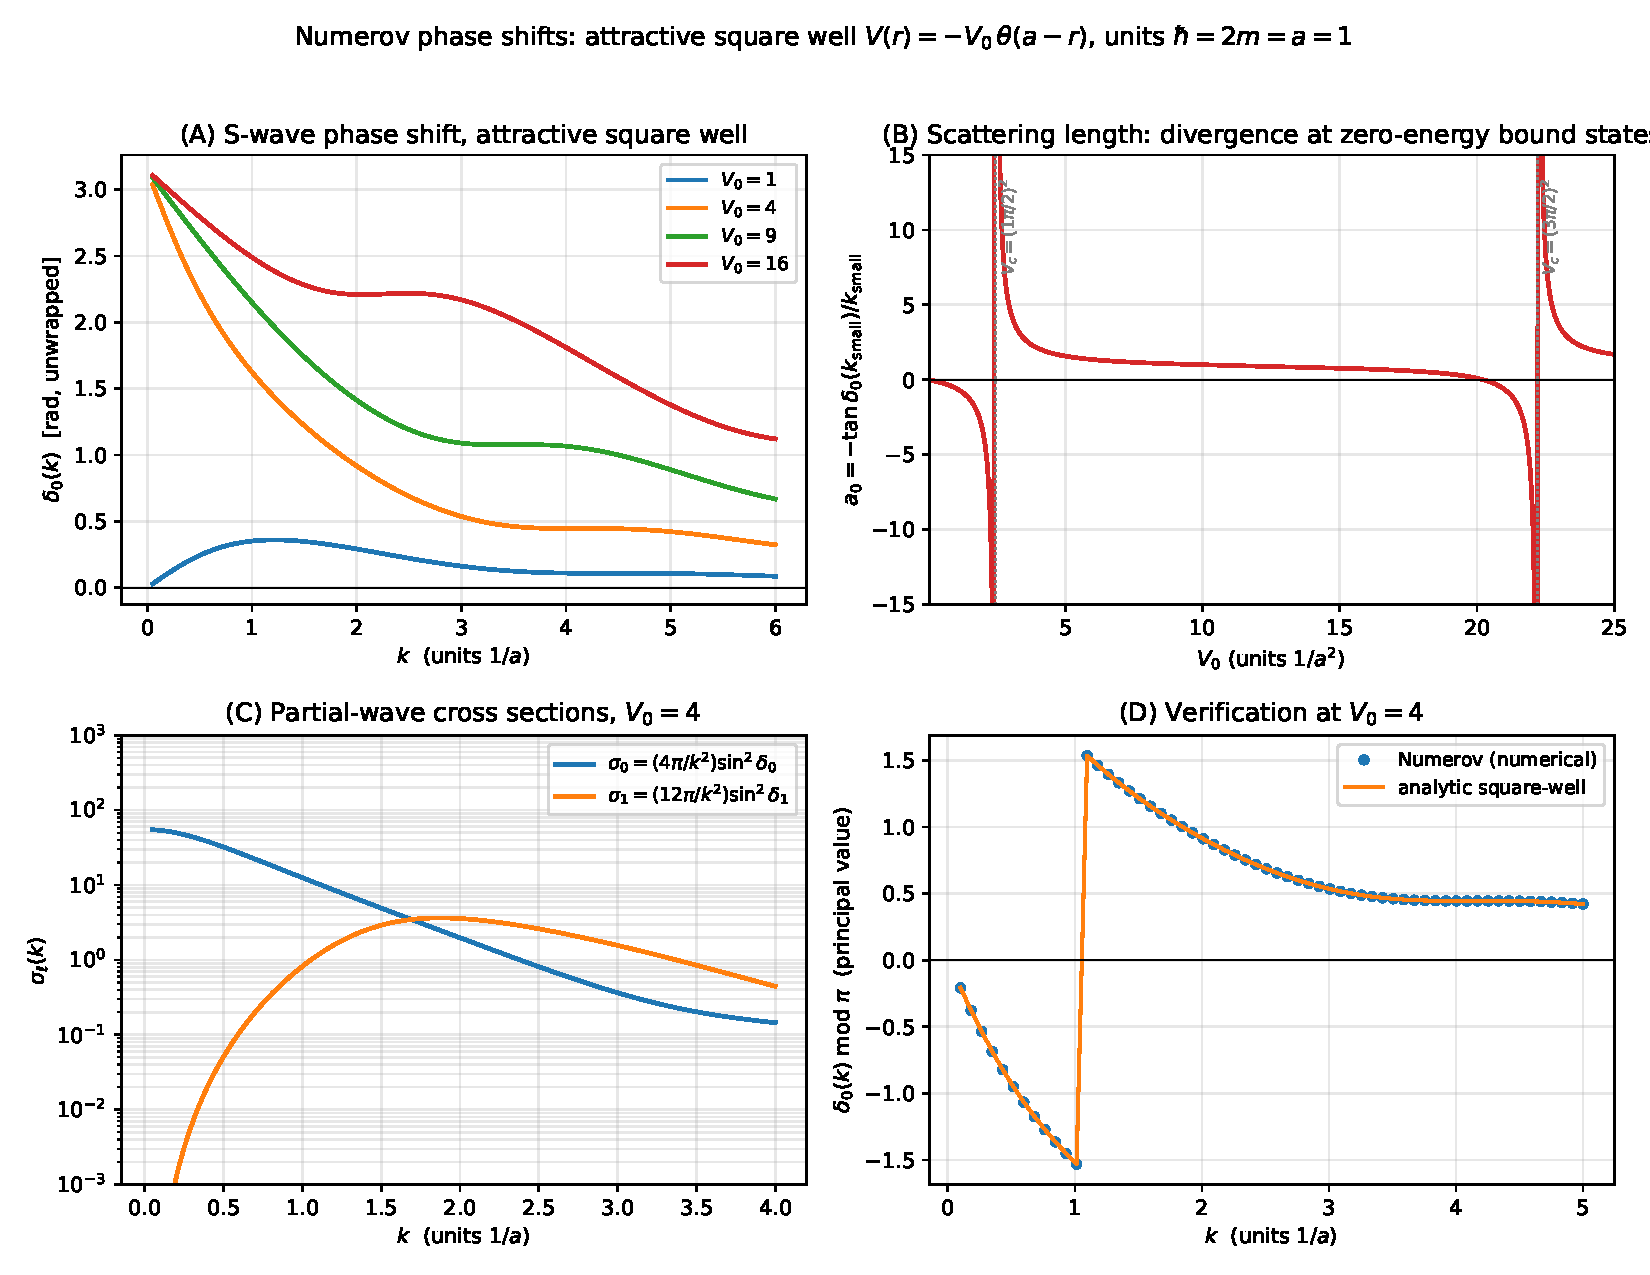
\includegraphics[width=0.95\linewidth]{ch10_numerov_phase}
    \caption{Numerov 法对吸引方势阱 $V(r)=-V_0\,\theta(a-r)$
    （单位 $\hbar=2m=a=1$）的 $s$、$p$ 波相移与截面。
    (A) $V_0=1,4,9,16$ 时的 $\delta_0(k)$（解 $\bmod\pi$ 后用
    \texttt{np.unwrap} 连续化）。$V_0=1<(\pi/2)^2\approx2.467$
    时无 $s$ 波束缚态，$\delta_0(0)=0$；$V_0=4,9,16$ 均处于
    $((\pi/2)^2,(3\pi/2)^2)$ 之间故各有 $1$ 个 $s$ 波束缚态，
    $\delta_0(0)\to\pi$，与 Levinson 定理 $\delta_0(0)=n_0\pi$
    （$n_0$ 为 $s$ 波束缚态数）一致。
    (B) 散射长度 $a_0=-\lim_{k\to0}\tan\delta_0(k)/k$ 作为 $V_0$
    的函数；图中两条灰虚线 $V_c=(\pi/2)^2,(3\pi/2)^2$ 处 $a_0$
    发散，对应零能束缚态新出现的阈值。
    (C) $V_0=4$ 时分波截面
    $\sigma_\ell(k)=(4\pi/k^2)(2\ell+1)\sin^2\delta_\ell(k)$
    （对数刻度）；低能区 $\sigma_0\propto a_0^2$ 占主导，
    $\sigma_1$ 由 $k^4$ 阈值压低。
    (D) $V_0=4$ 时 Numerov 数值（蓝点）与解析公式
    $\tan(ka+\delta_0)=(k/K)\tan(Ka)$，$K=\sqrt{k^2+V_0}$
    （橙线，主值分支）的逐点对比。}
    \label{fig:numexp-ch10}
\end{figure}

\subsection*{物理讨论}
\paragraph{Levinson 定理。}
图~\ref{fig:numexp-ch10}(A) 直接验证 $\delta_\ell(0)=n_\ell\pi$：
$V_0=1$ 时 $n_0=0$、$\delta_0(0)=0$；$V_0=4,9,16$ 三者落在同一
$s$ 波束缚态阈值区间 $((\pi/2)^2,(3\pi/2)^2)\approx(2.467,22.207)$
内，$n_0=1$、$\delta_0(0)=\pi$。每跨过一个阈值
$V_c=((2n+1)\pi/2)^2$，$\delta_0(0)$ 跳一个 $\pi$，与
\eqref{eq:pw-Levinson} 完全一致。

\paragraph{散射长度发散。}
图~\ref{fig:numexp-ch10}(B) 展示了 $a_0(V_0)$ 在
$V_c=(\pi/2)^2,(3\pi/2)^2$ 附近的极点，对应零能束缚态出现：
$a_0\to-\infty$（束缚态即将形成）→ 出现束缚态后 $a_0\to+\infty$
→ 回落至有限值。这是有效程展开
\[
  k\cot\delta_0(k)=-\frac{1}{a_0}+\frac12 r_0 k^2+\cdots
\]
中 $a_0$ 的奇异行为，物理上对应弱束缚极限下的“共振增强”——
低能截面 $\sigma_0\to 4\pi a_0^2$ 趋于无穷，正是冷原子物理中
Feshbach 共振、核物理中氘核虚态等现象的方势阱模型对应物。

\paragraph{低分波主导与解析比对。}
图~\ref{fig:numexp-ch10}(C) 展示低能区 $\sigma_0\gg\sigma_1$，
来源于离心位垒造成的 $\sigma_\ell\propto k^{4\ell}$ 阈值行为；
随 $k$ 增大高分波逐次开启，$ka\sim 1$ 起 $\sigma_1$ 与 $\sigma_0$
可比。图~\ref{fig:numexp-ch10}(D) 显示 Numerov 数值与方势阱
$s$ 波解析公式在主值分支上完全吻合（误差 $\lesssim 10^{-3}$，
与步长 $h=10^{-3}$ 的 $\mathcal O(h^4)$ 全局精度一致），
说明该数值方案可靠地推广到任意（球对称）势 $V(r)$。

\chapter{Coulomb 散射 (Coulomb Scattering)}\label{ch:coulomb}

到目前为止，本书所发展的散射理论 —— 包括第~\ref{ch:Smat1P} 章中
M{\o}ller 算符和 $\Smat$ 矩阵的定义、第~\ref{ch:stationary} 章中
定态散射波函数 $\inn{\vec x}{\vec p+}$ 的渐近形式、第~\ref{ch:partial}
章中相移 $\delta_\ell$ 与分波振幅的引入，以及第~\ref{ch:born} 章中
Born 级数的收敛 —— 都建立在一个核心假设之上：势 $V(r)$ 满足
\emph{短程}条件，例如 $r V(r)\to 0$ 当 $r\to\infty$。这一条件
保证了：自由演化 $\rme^{-\rmi H_0 t/\hbar}$ 能正确地描写在
$t\to\pm\infty$ 时散射粒子的渐近运动；定态波函数具有
``入射平面波 $+$ 球面外向波'' 的标准结构；分波相移 $\delta_\ell$
以及振幅 $f(\theta)$ 都是良定义的。

但是宇宙中最重要、最常见的相互作用之一 —— 两个带电粒子之间的
\emph{Coulomb 相互作用} $V(r)=e_1 e_2/r$ —— \emph{并不}满足上述短程
假设。$1/r$ 衰减得太慢：经典地讲，即使两粒子相距任意远，库仑力
依然在拉拽它们，导致散射轨道永远不能被视为``自由的''；量子地讲，
渐近条件 $\Op U(t)|\psi\rangle\to \Op U_0(t)|\psi_{\mathrm{in/out}}\rangle$
失效；定态解中也会出现额外的对数相位 $\eta\ln(\cdots)$。
因此这一章我们必须重新审视：在 Coulomb 势下散射理论应该如何
被修正，以便依旧给出有意义的可观测量（截面、相移、相位等）。

本章主要参考 Taylor《Scattering Theory》第 14 章 14-a, 14-b 节，
并把其中的物理结构与第~\ref{ch:partial} 章的分波框架、第~\ref{ch:born}
章的 Born 近似、以及第~\ref{ch:analytic} 章的解析延拓做对照。
我们将看到：尽管纯 Coulomb 没有``通常意义''的散射振幅，
但通过对渐近动力学的合理修正（Dollard 修正 M{\o}ller 算符），
或通过``屏蔽 $+$ 取极限''的物理论证，仍然可以建立一个完全自洽且
能给出 Rutherford 公式的散射理论。最后我们把短程力加在 Coulomb 之上，
解释 $p$-$p$、$\alpha$-核等实验中振幅 $f=f_C+f_N$ 的标准做法。

\section{Coulomb 势的特殊性}\label{sec:coulomb-special}

考虑两个电荷为 $e_1,e_2$ 的带电粒子在质心系下的相对运动，势能为
\begin{equation}
  V(r)=\frac{e_1 e_2}{r},\qquad r=|\vec x|.
  \label{eq:coulomb-V}
\end{equation}
我们之前所有定理（M{\o}ller 算符的存在性、$\Smat$ 的幺正性、
分波相移的良定义、Born 级数的收敛、Lippmann--Schwinger 方程的
迭代解、Levinson 定理等）都依赖于条件
\begin{equation}
  r\,V(r)\xrightarrow[r\to\infty]{}0,
  \label{eq:coulomb-shortrange-cond}
\end{equation}
而 $r\cdot e_1 e_2/r=e_1 e_2$ 是非零常数，故 \eqref{eq:coulomb-shortrange-cond}
不成立。直接的后果是：

\begin{enumerate}
  \item \textbf{渐近条件失效}：第~\ref{ch:Smat1P} 章中的渐近条件
  \begin{equation}
    \Op U(t)|\psi\rangle\xrightarrow[t\to\pm\infty]{}\Op U_0(t)|\psi_{\mathrm{out/in}}\rangle,
    \qquad \Op U_0(t)=\rme^{-\rmi \Op H_0 t/\hbar}
    \label{eq:coulomb-asymp-fail}
  \end{equation}
  对 Coulomb 势\emph{不再成立}：自由演化 $\Op U_0(t)$ 不能
  正确产生 Coulomb 散射的渐近行为。

  \item \textbf{径向解的对数畸变}：径向 Schr\"odinger 方程
  \begin{equation}
    \left[\frac{\rmd^2}{\rmd r^2}-\frac{\ell(\ell+1)}{r^2}
      -\frac{2m e_1 e_2}{\hbar^2 r}+k^2\right]y_\ell(r)=0
    \label{eq:coulomb-radial}
  \end{equation}
  的解在 $r\to\infty$ 时不再趋于 $\sin(kr-\ell\pi/2+\delta_\ell)$，
  而是出现一个对数相位 $\propto \ln r$ —— 即：
  \begin{equation}
    y_\ell(r)\sim \mathrm{const}\times\sin\!\left(kr-\eta\ln 2kr-\frac{\ell\pi}{2}+\sigma_\ell\right),
    \qquad r\to\infty,
    \label{eq:coulomb-radial-asymp}
  \end{equation}
  其中无量纲量
  \begin{equation}
    \boxed{\;\eta\equiv\frac{m e_1 e_2}{\hbar^2 k}=\frac{e_1 e_2}{\hbar v}\;}
    \label{eq:coulomb-eta-def}
  \end{equation}
  称为 Sommerfeld 参数。

  \item \textbf{Born 近似发散}：直接对 \eqref{eq:coulomb-V} 计算 Born 振幅
  \begin{equation}
    f^{(1)}(\vec q)=-\frac{2m}{\hbar^2 q}\int_0^\infty\!\rmd r\, r\sin(qr)\,V(r)
                 =-\frac{2m e_1 e_2}{\hbar^2 q}\int_0^\infty\!\rmd r\,\sin(qr)
    \label{eq:coulomb-born-divergent}
  \end{equation}
  得到一个不收敛的振荡积分，反映纯 Coulomb 势没有``通常意义''的振幅。
\end{enumerate}

\begin{remark}[物理上的处方]
现实中的 Coulomb 势永远不是``纯'' Coulomb：在 Rutherford 实验里
金核的 Coulomb 场被原子电子在埃 (\AA) 量级屏蔽；星际空间中带电粒子
的库仑场也被周围等离子体屏蔽到米量级。因此一个物理上合理的
出路是：先把 \eqref{eq:coulomb-V} 在某个大半径 $\rho$ 处截断
（或指数屏蔽），算出有限的振幅与截面，再考察 $\rho\to\infty$ 极限。
我们将看到，截面（除前向 $\theta=0$ 外）有良好的极限，而振幅
依赖于屏蔽方式 —— 这一现象本身就是 Coulomb ``长程性''的体现。
\end{remark}

\section{修正的 M{\o}ller 算符（Dollard 处方）}\label{sec:coulomb-moller}

本节给出处理 Coulomb 长程性的第二种、更具数学严格性的途径：
修正渐近动力学。这一思想由 Dollard (1964) 提出，并由 Amrein 等人
在七十年代发展为完整理论（参见 Taylor §14-a 注释）。

\subsection{对数畸变的来源}

直观地说：在纯 Coulomb 势下，一个朝 $z$ 方向飞出的粒子，其动量
$\vec p$ 几乎不变，但相位却在不断累积。考虑半经典近似（WKB），
波函数沿轨道的相位为
\begin{equation}
  \frac{1}{\hbar}\!\int^t\!\rmd t'\,\bigl[E-V(r(t'))\bigr]
  \approx\frac{Et}{\hbar}-\frac{1}{\hbar}\!\int^t\!\rmd t'\,\frac{e_1 e_2}{v t'}
  =\frac{Et}{\hbar}-\eta\ln|t|+\mathrm{const}.
\end{equation}
也就是说，自由演化 $\rme^{-\rmi H_0 t/\hbar}$ 比真实演化少了一项
$-\rmi\eta\ln|t|$。Dollard 的想法是：把这一对数相位\emph{显式地}
吸收进``参考''演化算符里，于是修正后的渐近自由演化与真实
Coulomb 演化之间就能匹配。

\subsection{Dollard 修正演化算符}

定义
\begin{empheq}[box=\fbox]{equation}
  \Op U_D(t)\;\equiv\;\exp\!\left[-\frac{\rmi}{\hbar}\Op H_0 t
  -\rmi\,\eta(\Op H_0)\,\ln\!\bigl(2\Op H_0|t|/\hbar\bigr)\,\sgn(t)\right],
  \label{eq:coulomb-dollard-U}
\end{empheq}
其中 $\eta(\Op H_0)=m e_1 e_2/(\hbar^2 \sqrt{2m\Op H_0/\hbar^2})$ 是把
\eqref{eq:coulomb-eta-def} 中的 $k$ 替换为算符 $\sqrt{2\Op H_0}/\hbar$
后得到的算符函数（在动量基下其特征值即 $\eta(k)=m e_1 e_2/\hbar^2 k$）。
注意 $[\Op H_0,\eta(\Op H_0)]=0$，故 \eqref{eq:coulomb-dollard-U} 可以
直接对角化。

\subsection{修正 M{\o}ller 算符 $\Op\Omega^C_\pm$}

对应地，定义\textbf{Coulomb 修正 M{\o}ller 算符}
\begin{empheq}[box=\fbox]{align}
  \Op\Omega^C_\pm\;\psi\;
  &\equiv\;\lim_{t\to\mp\infty}\Op U(t)^\dagger\,\Op U_D(t)\,\psi,
  \quad\text{即}\quad \Op U(t)\Op\Omega^C_\pm\psi
  \xrightarrow[t\to\pm\infty]{}\Op U_D(t)\psi,
  \label{eq:coulomb-omega-C}
\end{empheq}
其中 $\Op U(t)=\rme^{-\rmi\Op H t/\hbar}$ 是真实 Coulomb 演化。
Dollard 证明了：在 \eqref{eq:coulomb-V} 之下，强极限
\eqref{eq:coulomb-omega-C} \emph{存在}且 $\Op\Omega^C_\pm$ 是
等距的；进一步可以定义\textbf{Coulomb 散射算符}
\begin{equation}
  \Op{S}^C\;\equiv\;(\Op\Omega^C_+)^\dagger\,\Op\Omega^C_-,
\end{equation}
它是幺正算符，扮演着第~\ref{ch:Smat1P} 章中 $\Smat$ 的角色。

\begin{remark}
``渐近条件'' \eqref{eq:coulomb-asymp-fail} 实际上比实验所要求的
强得多：实验中只测量动量、动能、自旋等\emph{与 $\Op H_0$ 对易}的可观测量
的渐近极限，而不要求整个态向量与一个自由演化态在 Hilbert 空间中
重合。修正 M{\o}ller 算符正好削弱了渐近条件，使其可以容纳长程
势，同时不影响实验可观测量。
\end{remark}

\begin{remark}[与短程理论的兼容性]
若同时存在短程势 $V_{\mathrm{sr}}(r)$（满足 $rV_{\mathrm{sr}}\to 0$）：
$V=e_1 e_2/r+V_{\mathrm{sr}}$，则 \eqref{eq:coulomb-omega-C} 依然给出
良定义的 $\Op\Omega^C_\pm$，且短程部分的散射振幅可以与 Coulomb 部分
分离（见 \S\ref{sec:coulomb-plus-shortrange}）。
\end{remark}

\section{Coulomb 波函数：坐标空间表象}\label{sec:coulomb-wave}

我们现在求解定态 Schr\"odinger 方程
\begin{equation}
  \left(-\frac{\hbar^2}{2m}\nabla^2+\frac{e_1 e_2}{r}\right)\psi(\vec x)
  =E\,\psi(\vec x),\qquad E=\frac{\hbar^2 k^2}{2m}>0.
  \label{eq:coulomb-schrodinger}
\end{equation}
取入射方向沿 $\hat z$，并写 $\psi^+_C(\vec x)$ 表示``带入射平面波''
的散射定态（对应 $\Op\Omega^C_+|\vec p\rangle$）。已知该方程在
抛物线坐标 $\xi=r-z,\eta_p=r+z$ 下分离变量，解可以用合流超几何
函数 ${}_1F_1(a;c;z)$ 表达。

\subsection{解的形式}

直接验证（参见 Messiah《Quantum Mechanics》Ch.\ XI 附录 B），
\begin{empheq}[box=\fbox]{equation}
  \boxed{\;\psi^+_C(\vec x)\;=\;\rme^{-\pi\eta/2}\,\Gamma(1+\rmi\eta)\,
    \rme^{\rmi\vec k\cdot\vec x}\,
    {}_1F_1\!\bigl(-\rmi\eta;\,1;\,\rmi(kr-\vec k\cdot\vec x)\bigr)\;}
  \label{eq:coulomb-psi-plus}
\end{empheq}
是 \eqref{eq:coulomb-schrodinger} 的解。证明的要点是把
$\psi^+_C=\rme^{\rmi\vec k\cdot\vec x}\,F(\xi)$（$\xi=r-z$）代入，
得到合流超几何方程
\[
  \xi F''(\xi)+(1-\rmi k\xi)F'(\xi)+\eta k F(\xi)=0,
\]
其在 $\xi=0$ 处正则的解即 ${}_1F_1(-\rmi\eta;1;\rmi k\xi)$。归一化
因子 $\rme^{-\pi\eta/2}\Gamma(1+\rmi\eta)$ 是为了让 \eqref{eq:coulomb-psi-plus}
在 $\eta\to 0$ 极限下回到 $\rme^{\rmi\vec k\cdot\vec x}$。

\subsection{渐近形式}

利用 ${}_1F_1$ 在 $|z|\to\infty$ 时的渐近展开
\begin{align}
  {}_1F_1(a;c;z)&\sim\frac{\Gamma(c)}{\Gamma(c-a)}(-z)^{-a}+\frac{\Gamma(c)}{\Gamma(a)}\rme^z z^{a-c}
\end{align}
（在 $\arg(-z)<\pi$ 的扇形内成立），代入 \eqref{eq:coulomb-psi-plus}
并取 $r-z\to\infty$（即排除前向 $\theta=0$）得到
\begin{empheq}[box=\fbox]{align}
  \psi^+_C(\vec x)\;\xrightarrow{r\to\infty}\;
  &\;\rme^{\rmi[kz+\eta\ln k(r-z)]} \nonumber\\
  &\quad+\;f_C(\theta)\,\frac{\rme^{\rmi[kr-\eta\ln 2kr]}}{r},
  \label{eq:coulomb-psi-asymp}
\end{empheq}
其中
\begin{empheq}[box=\fbox]{equation}
  f_C(\theta)\;=\;-\,\frac{\eta}{2k\sin^2(\theta/2)}\,
  \exp\!\left[-\rmi\eta\ln\sin^2(\theta/2)+2\rmi\sigma_0\right],
  \label{eq:coulomb-fC}
\end{empheq}
被称为 \emph{Coulomb 散射振幅}，$\sigma_0=\arg\Gamma(1+\rmi\eta)$
是 $\ell=0$ 的 Coulomb 相移。

\begin{remark}[与短程情形的对照]
\eqref{eq:coulomb-psi-asymp} 与短程定态 $\psi^+(\vec x)\to
\rme^{\rmi\vec k\cdot\vec x}+f(\theta)\rme^{\rmi kr}/r$ 比较：
\begin{itemize}
  \item ``入射波'' $\rme^{\rmi[kz+\eta\ln k(r-z)]}$ 多出一个对数畸变
    $\eta\ln k(r-z)$ —— 反映 Coulomb 长程力对入射粒子相位的修改；
  \item ``散射波'' $f_C(\theta)\rme^{\rmi[kr-\eta\ln 2kr]}/r$
    多出对数相位 $-\eta\ln 2kr$ —— 同源；
  \item 振幅本身 $f_C(\theta)$ 也带有对数相位
    $-\rmi\eta\ln\sin^2(\theta/2)$。
\end{itemize}
正因为有这些对数相位，``散射振幅''没有像短程情形那样唯一地
由 $\Smat$-矩阵元定义；不过下面会看到，截面只看 $|f_C|^2$，
对数相位不出现。
\end{remark}

\section{Coulomb 散射振幅的推导}\label{sec:coulomb-fC-derivation}

我们对 \eqref{eq:coulomb-fC} 给一个稍详细的推导。设
$\vec k=k\hat z$，则 $\vec k\cdot\vec x=kz$，$kr-\vec k\cdot\vec x=k(r-z)$。
记 $u=\rmi k(r-z)$，则 \eqref{eq:coulomb-psi-plus} 即
\[
  \psi^+_C=\rme^{-\pi\eta/2}\Gamma(1+\rmi\eta)\rme^{\rmi kz}\,{}_1F_1(-\rmi\eta;1;u).
\]
由合流超几何渐近公式（取 $a=-\rmi\eta,\,c=1$），
\begin{align}
  {}_1F_1(-\rmi\eta;1;u)
  &\sim\frac{1}{\Gamma(1+\rmi\eta)}(-u)^{\rmi\eta}\Bigl[1+O(u^{-1})\Bigr]\nonumber\\
  &\quad+\frac{\rme^u u^{-\rmi\eta-1}}{\Gamma(-\rmi\eta)}\Bigl[1+O(u^{-1})\Bigr].
\end{align}
直接代入：

\paragraph{第一项（``入射''部分）.}
由 $-u=-\rmi k(r-z)=k(r-z)\rme^{-\rmi\pi/2}$，所以
$(-u)^{\rmi\eta}=[k(r-z)]^{\rmi\eta}\rme^{\eta\pi/2}=\rme^{\eta\pi/2}\rme^{\rmi\eta\ln k(r-z)}$。
将其乘以 $\rme^{-\pi\eta/2}\Gamma(1+\rmi\eta)$ 与 $1/\Gamma(1+\rmi\eta)$，
归一化因子相消，得到
\[
  \psi^+_C\Big|_{\text{第一}}\sim\rme^{\rmi[kz+\eta\ln k(r-z)]},
\]
即 \eqref{eq:coulomb-psi-asymp} 中的入射部分。

\paragraph{第二项（``散射''部分）.}
由 $\rme^u=\rme^{\rmi k(r-z)}$，结合 $\rme^{\rmi kz}\rme^u=\rme^{\rmi kr}$，
以及 $u^{-\rmi\eta-1}=[\rmi k(r-z)]^{-\rmi\eta-1}$。
在 $r-z=2r\sin^2(\theta/2)$（$\theta$ 为 $\hat z$ 与 $\hat r$ 的夹角）下，
\[
  u^{-\rmi\eta-1}=\frac{1}{\rmi k(r-z)}\rme^{-\rmi\eta\ln[2kr\sin^2(\theta/2)]}\rme^{\eta\pi/2}.
\]
合并并使用 $\Gamma$ 函数恒等式 $\Gamma(-\rmi\eta)=\Gamma(1-\rmi\eta)/(-\rmi\eta)$ 与
$\Gamma(1+\rmi\eta)\Gamma(1-\rmi\eta)=\pi\eta/\sinh(\pi\eta)$，把
$|\Gamma(1+\rmi\eta)|^2=\pi\eta/\sinh(\pi\eta)$ 转化为 $\rme^{-\pi\eta}$ 因子，
最终得到：
\begin{align}
  \psi^+_C\Big|_{\text{第二}}
  &\sim \frac{\Gamma(1+\rmi\eta)}{\Gamma(-\rmi\eta)}\,
    \frac{1}{\rmi k(r-z)}\,\rme^{\rmi[kr-\eta\ln 2kr]}\rme^{-\rmi\eta\ln\sin^2(\theta/2)}\nonumber\\
  &=\;f_C(\theta)\,\frac{\rme^{\rmi[kr-\eta\ln 2kr]}}{r},
\end{align}
其中通过 $\Gamma(1+\rmi\eta)/\Gamma(-\rmi\eta)=-\rmi\eta\,\Gamma(1+\rmi\eta)/\Gamma(1-\rmi\eta)
=-\rmi\eta\,\rme^{2\rmi\sigma_0}$（这里用了
$\sigma_0=\arg\Gamma(1+\rmi\eta)$，故 $\Gamma(1+\rmi\eta)=|\Gamma(1+\rmi\eta)|\rme^{\rmi\sigma_0}$）
化简，并代入 $r-z=2r\sin^2(\theta/2)$，恰好得到 \eqref{eq:coulomb-fC}。
\hfill$\Box$

\begin{remark}
推导中三个非平凡的细节：(i) $\rme^{-\pi\eta/2}$ 与第二项中
$\rme^{\eta\pi/2}$ 因子相消；(ii) $1/(r-z)$ 中的 $1/[2\sin^2(\theta/2)]$
正是 Rutherford 角分布；(iii) $\arg[\Gamma(1+\rmi\eta)/\Gamma(1-\rmi\eta)]
=2\sigma_0$ 是相移 $\sigma_0$ 出现于振幅中的源头。
\end{remark}

\section{微分截面：Rutherford 公式}\label{sec:coulomb-Rutherford}

对 \eqref{eq:coulomb-fC} 取模方：
\begin{empheq}[box=\fbox]{equation}
  \frac{\rmd\sigma_C}{\rmd\Omega}\;=\;|f_C(\theta)|^2
  \;=\;\frac{\eta^2}{4k^2\sin^4(\theta/2)}
  \;=\;\frac{m^2 e_1^2 e_2^2}{4 p^4\sin^4(\theta/2)}.
  \label{eq:coulomb-Rutherford}
\end{empheq}
这正是著名的 \textbf{Rutherford 公式}（$p=\hbar k$，$E=p^2/2m$）。

\begin{remark}[惊人巧合]
Rutherford 公式 \eqref{eq:coulomb-Rutherford} 同时出现在三个层级：
经典 Rutherford 散射、量子 Born 一阶近似（如果对屏蔽 Coulomb 取
$\rho\to\infty$ 极限）、以及上面的精确合流超几何解。三者完全一致，
是 Coulomb 势的高度对称性的反映（实际上来源于 $1/r$ 势的隐藏
$O(4)$ 对称性，与氢原子简并性的 Pauli-Lenz 矢量是同源的）。
\end{remark}

\subsection{$\theta\to 0$ 发散与无穷大总截面}

\eqref{eq:coulomb-Rutherford} 在 $\theta\to 0$ 时发散 $\propto 1/\theta^4$，
故\emph{总截面}
\begin{equation}
  \sigma_{\mathrm{tot}}=\int\!\rmd\Omega\,\frac{\rmd\sigma_C}{\rmd\Omega}
  =\int_0^\pi 2\pi\sin\theta\,\rmd\theta\;\frac{\eta^2}{4k^2\sin^4(\theta/2)}
\end{equation}
\emph{发散}。物理上：库仑力的长程性意味着任意大碰撞参数 $b$ 处粒子
仍被偏转一个有限角度，故总散射概率无界。

更精细地：经典 Rutherford 散射有 $\theta=2\arctan(\eta/kb)$，
故 $\theta\to 0\Leftrightarrow b\to\infty$；这一对应在量子情形依然
（半经典地）成立。这也解释了为什么前向 $\theta\approx 0$ 对屏蔽
方式特别敏感：``大 $b$ 粒子''被屏蔽刚刚到达的位置（或更外）所
影响最大。一旦在角分布上避开 $\theta=0$ 的小邻域，截面与屏蔽方式
无关 —— 这就是 Taylor §14-a 论证的核心。

\subsection{屏蔽方式无关性的简单证明}

考虑两种屏蔽：(a) 指数屏蔽 $V_a=(e_1 e_2/r)\rme^{-r/\rho}$；
(b) 锐截断 $V_b=(e_1 e_2/r)\Theta(\rho-r)$。Born 振幅分别为
\begin{align}
  f^{(1)}_a(\vec q)&=-\frac{2m e_1 e_2}{\hbar^2(q^2+\rho^{-2})}\xrightarrow{\rho\to\infty}-\frac{2m e_1 e_2}{\hbar^2 q^2},\\
  f^{(1)}_b(\vec q)&=-\frac{2m e_1 e_2}{\hbar^2 q^2}(1-\cos q\rho).
\end{align}
两者差别为 $\propto\cos q\rho$。在 $q\rho\gg 1$（$\rho$ 远大于德布罗意波长）时
$\cos q\rho$ 是一个高频振荡函数，在任何合理宽度的入射波包上做角积分时
积分为零。因此在\emph{可观测层面}上两种屏蔽给出相同的截面 $\rmd\sigma/\rmd\Omega
=|2me_1e_2/(\hbar^2 q^2)|^2=\eta^2/(4k^2\sin^4(\theta/2))$，
与 \eqref{eq:coulomb-Rutherford} 一致。

\section{Coulomb 分波分析}\label{sec:coulomb-partial}

我们现在转向角动量分析。把 \eqref{eq:coulomb-radial} 写成约化形式
$y_\ell=r R_\ell$：
\begin{equation}
  y_\ell''+\left[k^2-\frac{\ell(\ell+1)}{r^2}-\frac{2k\eta}{r}\right]y_\ell=0,
  \label{eq:coulomb-radial-eta}
\end{equation}
其中 $\eta$ 由 \eqref{eq:coulomb-eta-def} 给出。

\subsection{正则解 $F_\ell$ 与不规则解 $G_\ell$}

\eqref{eq:coulomb-radial-eta} 的两个线性独立解传统上记作：

\begin{itemize}
  \item \textbf{正则 Coulomb 函数} $F_\ell(\eta,kr)$：在 $r\to 0$ 时
  按 $\sim (kr)^{\ell+1}$ 趋于零，故对应物理上``在原点正则''的解。
  其渐近行为：
  \begin{empheq}[box=\fbox]{equation}
    F_\ell(\eta,kr)\;\xrightarrow{r\to\infty}\;\sin\!\left(kr-\eta\ln 2kr-\frac{\ell\pi}{2}+\sigma_\ell\right),
    \label{eq:coulomb-Flasymp}
  \end{empheq}

  \item \textbf{不规则 Coulomb 函数} $G_\ell(\eta,kr)$：在 $r\to 0$ 时
  发散 $\sim (kr)^{-\ell}$，但渐近为
  \begin{equation}
    G_\ell(\eta,kr)\;\xrightarrow{r\to\infty}\;\cos\!\left(kr-\eta\ln 2kr-\frac{\ell\pi}{2}+\sigma_\ell\right).
    \label{eq:coulomb-Glasymp}
  \end{equation}
\end{itemize}

注意 \eqref{eq:coulomb-Flasymp}, \eqref{eq:coulomb-Glasymp} 中
\emph{对数畸变项} $-\eta\ln 2kr$ 是显式的；这是 Coulomb 与短程
Riccati--Bessel 函数 $\hat\jmath_\ell(kr)\to\sin(kr-\ell\pi/2)$
的本质区别。

\subsection{Coulomb 相移 $\sigma_\ell$}

\textbf{Coulomb 相移}（``库仑相位''）由
\begin{empheq}[box=\fbox]{equation}
  \boxed{\;\sigma_\ell\;=\;\arg\Gamma(\ell+1+\rmi\eta)\;}
  \label{eq:coulomb-sigmal}
\end{empheq}
给出。证明可以基于 \eqref{eq:coulomb-radial-eta} 的合流超几何
表达：
\[
  F_\ell(\eta,\rho)=2^\ell\,\rme^{-\pi\eta/2}\,\frac{|\Gamma(\ell+1+\rmi\eta)|}{(2\ell+1)!}
  \rho^{\ell+1}\rme^{\rmi\rho}\,{}_1F_1(\ell+1-\rmi\eta;\,2\ell+2;\,-2\rmi\rho),
\]
（$\rho=kr$）然后用合流超几何渐近公式把 $\rho\to\infty$ 的相位提取
出来，即得 \eqref{eq:coulomb-Flasymp} 与 \eqref{eq:coulomb-sigmal}。
特别 $\ell=0$ 时 $\sigma_0=\arg\Gamma(1+\rmi\eta)$。

\begin{remark}
\eqref{eq:coulomb-sigmal} 显示 $\sigma_\ell$ 在所有 $\ell$ 都\emph{非零}
（除非 $\eta=0$）。这与短程势相移随 $\ell\to\infty$ 趋于零的图像截然不同
—— 反映 Coulomb 长程力对所有分波分量都起作用。
\end{remark}

\subsection{对数相位的不可消除性}

为什么不可以简单地把 \eqref{eq:coulomb-Flasymp} 中的对数项 $-\eta\ln 2kr$
``并入''总相位 $\sigma_\ell$？因为它依赖 $r$。任何物理意义的
``相移''都必须是常数（与 $r$ 无关）。这暗示：在 Coulomb 情形，
``相移''这个概念本身要被重新定义 —— 可以把它定义为
$F_\ell$ 与所谓 \emph{Coulomb-Bessel 函数}（即把对数项扣掉的
``参考''解）之间的相位差，但相位差本身并不进入 $r$ 的相位。
重要的是\eqref{eq:coulomb-sigmal} 给出的常数部分 $\sigma_\ell$
进入散射振幅。

\subsection{Coulomb 振幅的分波展开（一致性检验）}

我们应该可以通过分波展开重新得到 \eqref{eq:coulomb-fC}：
\begin{equation}
  f_C(\theta)=\frac{1}{2\rmi k}\sum_{\ell=0}^\infty (2\ell+1)\,\bigl(\rme^{2\rmi\sigma_\ell}-1\bigr)\,P_\ell(\cos\theta).
  \label{eq:coulomb-fC-partial}
\end{equation}
这一级数实际上\emph{不收敛}（因为 $\sigma_\ell\to\eta\ln\ell+\mathrm{const}$
对大 $\ell$ 不衰减），需要在 Abel 求和或解析正规化的意义下理解。
其闭式正是 \eqref{eq:coulomb-fC}。这与短程情形的分波振幅
$f(\theta)=(2\rmi k)^{-1}\sum (2\ell+1)(\rme^{2\rmi\delta_\ell}-1)P_\ell$
形式上完全平行，只是相移 $\delta_\ell\to\sigma_\ell$。

\section{Coulomb 加短程势}\label{sec:coulomb-plus-shortrange}

现在考虑实际中最常见的情况：在 $1/r$ Coulomb 之上叠加一个短程
势（如 $p$-$p$ 散射中 Coulomb $+$ 强相互作用，电子-质子散射中
Coulomb $+$ 自旋-轨道，等等）：
\begin{equation}
  V(r)=\frac{e_1 e_2}{r}+V_{\mathrm{sr}}(r),\qquad
  V_{\mathrm{sr}}(r)=0\;\text{当}\;r>a.
  \label{eq:coulomb-V-sr}
\end{equation}
我们继续使用截断半径 $\rho\gg a$ 的处方：在 $r<a$ 是``Coulomb $+$
短程''，在 $a<r<\rho$ 是纯 Coulomb，在 $r>\rho$ 无势。

\subsection{额外相移 $\delta_\ell^N$}

在区域 $a<r<\rho$ 中，径向波函数是 $F_\ell$ 与 $G_\ell$ 的线性组合：
\begin{equation}
  \psi_{\ell,p}(r)=\mathrm{const}\,\bigl[F_\ell(\eta,kr)+\tan\delta_\ell^N\,G_\ell(\eta,kr)\bigr],
  \quad a<r<\rho,
\end{equation}
其中 $\delta_\ell^N$ 衡量 $V_{\mathrm{sr}}$ 对波函数的修正。
由于短程力的相移对大 $\ell$ 衰减很快（$\ell>\ell_0\approx ka$
时基本为零），故 $\delta_\ell^N\ne 0$ 只有有限多个 $\ell$。

利用 \eqref{eq:coulomb-Flasymp}, \eqref{eq:coulomb-Glasymp} 的渐近，
$r\gtrsim a$ 时
\begin{equation}
  \psi_{\ell,p}(r)\propto\sin\!\left(kr-\eta\ln 2kr-\frac{\ell\pi}{2}
  +\sigma_\ell+\delta_\ell^N\right),
\end{equation}
即\textbf{总相移} $=\sigma_\ell+\delta_\ell^N-\eta\ln 2kr$（与
\eqref{eq:coulomb-radial-asymp} 比较）。其中 $\sigma_\ell+\delta_\ell^N$
中真正反映短程力效应的是 $\delta_\ell^N$。

\subsection{修正后的振幅 $f=f_C+f_N$}

按照 Taylor §14-b 的标准推导（在区域 $r>\rho$ 用入射 Hankel 与
出射 Hankel 表示，与 $r<\rho$ 的 Coulomb 解作匹配），得到的总振幅是
\begin{empheq}[box=\fbox]{equation}
  f(\theta)=f_C(\theta)+f_N(\theta),
  \label{eq:coulomb-f-total}
\end{empheq}
其中 $f_C$ 由 \eqref{eq:coulomb-fC} 给出，而\textbf{核子振幅}（短程
``附加''振幅）由
\begin{empheq}[box=\fbox]{equation}
  f_N(\theta)=\frac{1}{2\rmi k}\sum_{\ell=0}^{\ell_0}(2\ell+1)\,
  \rme^{2\rmi\sigma_\ell}\,\bigl(\rme^{2\rmi\delta_\ell^N}-1\bigr)\,P_\ell(\cos\theta)
  \label{eq:coulomb-fN}
\end{empheq}
给出。注意 \eqref{eq:coulomb-fN} 与短程纯散射振幅的差别：每一项
多了一个相位 $\rme^{2\rmi\sigma_\ell}$ —— 这反映短程散射``发生在
Coulomb 畸变波背景下''，是``Coulomb 修正的 Born 近似''或
``扭曲波 Born 近似 (DWBA)''的体现（DWBA 概念见 Taylor §14-c）。

\subsection{微分截面与干涉}

总截面为
\begin{equation}
  \frac{\rmd\sigma}{\rmd\Omega}=|f_C+f_N|^2=|f_C|^2+|f_N|^2+2\,\Re[f_C^* f_N],
  \label{eq:coulomb-sigma-cross}
\end{equation}
其中第一项是 Rutherford 项，第二项是``纯核子项''，第三项是
\emph{Coulomb-核子干涉项}。

\begin{example}[$p$-$p$ 散射，几 MeV]
低能 $p$-$p$ 散射中，$s$-波相移 $\delta_0^N$（核相移）很显著
而 Coulomb $\sigma_0$ 很小。此时 $f_N\approx (1/p)\rme^{\rmi\delta_0}\sin\delta_0$，
代入 \eqref{eq:coulomb-sigma-cross}：
\begin{align}
  \frac{\rmd\sigma}{\rmd\Omega}
  &=\Bigl(\frac{\rmd\sigma}{\rmd\Omega}\Bigr)_C
  +\frac{\sin^2\delta_0}{p^2}-\frac{m e_1 e_2}{p^3\sin^2(\theta/2)}\sin\delta_0
    \cos\!\bigl(\delta_0-2\eta\ln\sin(\theta/2)\bigr).
\end{align}
最后一项依赖于 $\delta_0$ 的\emph{符号}（即核力是吸引还是排斥），
故 Coulomb-核子干涉提供了\emph{相移符号信息} —— 这是单纯短程
散射所做不到的。
\end{example}

\begin{remark}[相位约定]
\eqref{eq:coulomb-fN} 中的 $\rme^{2\rmi\sigma_\ell}$ 是常见的``Coulomb
修正''标准约定。亦有文献定义 $f_N$ 时把这个相位放到 $f_C$ 一侧；
它影响截面只在 $f_C^* f_N$ 的干涉项相位上，需要约定一致。
\end{remark}

\section{Coulomb 束缚态：氢原子}\label{sec:coulomb-bound}

吸引性 Coulomb 势 $V(r)=-Ze^2/r$（$Ze^2>0$）支持无穷多个束缚态。
按第~\ref{ch:analytic} 章的视角，束缚态对应于分波 $S$ 矩阵元
$\mathsf{s}_\ell(p)$ 在正虚轴 $p=\rmi\kappa$（$\kappa>0$）上的极点。
对 Coulomb 而言 $\eta=mZe^2/(\hbar^2 k)\to-\rmi mZe^2/(\hbar^2\kappa)$
（吸引时 $e_1 e_2<0$，故记 $\eta_b\equiv mZe^2/\hbar^2\kappa>0$）。
$\sigma_\ell=\arg\Gamma(\ell+1+\rmi\eta)$ 在 $\eta=-\rmi\eta_b$ 处即
$\Gamma(\ell+1+\eta_b)$，发散于 $\ell+1+\eta_b=-n_r$ ($n_r=0,1,\dots$)：
\begin{equation}
  \eta_b=n,\qquad n\equiv n_r+\ell+1=1,2,3,\ldots,
\end{equation}
即 $\kappa_n=mZe^2/(\hbar^2 n)$。能量为
\begin{empheq}[box=\fbox]{equation}
  E_n=-\frac{\hbar^2\kappa_n^2}{2m}=-\frac{m Z^2 e^4}{2\hbar^2 n^2},
  \label{eq:coulomb-Ebound}
\end{empheq}
即著名的氢原子能级公式（$n$ 为主量子数）。

\begin{remark}
这个推导把氢原子的``束缚态分立谱''与散射的``Coulomb 相移''
统一在一个解析框架中：$\Gamma(\ell+1+\rmi\eta)$ 函数同时编码
散射相移 \eqref{eq:coulomb-sigmal} 和束缚态条件
\eqref{eq:coulomb-Ebound}。这一``散射 $+$ 束缚态''的统一是
解析延拓视角的强大例证（参见第~\ref{ch:analytic} 章）。
\end{remark}

\section{多粒子 Coulomb：三体问题与 Faddeev 困难}\label{sec:coulomb-3body}

最后简要提一个高级话题：当系统中有多个带电粒子两两通过 Coulomb
相互作用时（如 $e^-+\mathrm{H}\to e^-+e^-+p$ 的电离过程，或
$d+t\to n+\alpha$ 中的核-核库仑），渐近运动包含\emph{多重}
对数相位，每一对带电粒子都有一份。

\subsection{三体 Coulomb 渐近}

考虑三个带电粒子 $1,2,3$，电荷 $e_i$。在三粒子全部分离的渐近区
（``$3\to 3$'' 或``$3\to 2+1$'' 区域），相对动量 $\vec k_{ij}$
之间的 Coulomb 仍存在，故波函数渐近形式中要出现三个对数相位：
\begin{equation}
  \psi^+\;\sim\;\rme^{\rmi\sum_i\vec k_i\cdot\vec x_i}\,
  \prod_{i<j}\rme^{\rmi\eta_{ij}\ln(k_{ij}r_{ij}-\vec k_{ij}\cdot\vec r_{ij})}+\cdots
  \label{eq:coulomb-3body-asymp}
\end{equation}
这就是 Brauner-Briggs-Klar (BBK) 波函数的核心结构。

\subsection{Faddeev 方程的失效}

\textbf{Faddeev 方程}（多体散射的标准框架）的核心假设是：每个
两体子系的 $T$-矩阵是已知的、与其他粒子的存在无关。但在 Coulomb
情形，两体 Coulomb $T$-矩阵本身没有``通常意义''下的良定义
（如前所述 Born 积分发散），更重要的是 \eqref{eq:coulomb-3body-asymp}
中的对数相位\emph{无法}分解为两体 Coulomb 振幅的简单和。

具体地，Faddeev 算符 $\Op T_{ij}=\Op V_{ij}+\Op V_{ij}\Op G_0\Op T_{ij}$
中的 $\Op V_{ij}$ 是裸的 $1/r$，故迭代时产生与 \eqref{eq:coulomb-born-divergent}
同型的发散。
处理这一困难的方法包括：

\begin{itemize}
  \item \textbf{屏蔽-极限法}：先把 Coulomb 屏蔽到 $\rho$，对 Faddeev
    方程求解，再在物理量级取 $\rho\to\infty$，需要谨慎扣除发散相位
    （Alt-Sandhas 等人的工作）。
  \item \textbf{修正 Faddeev 方程}：把 Dollard 修正吸收到自由
    Green 函数 $\Op G_0\to\Op G_0^C$ 中（Merkuriev 等人）。
  \item \textbf{解析延拓}：把 Faddeev 方程在复 $\eta$ 平面上做
    解析延拓，再回到物理实轴。
\end{itemize}

这些技术超出本书范围，但它们的存在表明：长程 Coulomb 在多体
散射中是一个真正的难题，至今仍是活跃研究方向。

\section{本章小结}\label{sec:coulomb-summary}

\begin{itemize}
  \item Coulomb 势 $V=e_1 e_2/r$ 不满足短程条件 $rV\to 0$，导致
    标准渐近条件 \eqref{eq:coulomb-asymp-fail} 失效，Born 近似
    发散，相移定义出现对数畸变 $-\eta\ln 2kr$。

  \item 两条出路：(i) 物理上，``屏蔽 $+$ 取极限'' —— 截面有良好
    极限（Rutherford 公式 \eqref{eq:coulomb-Rutherford}）；
    (ii) 数学上，引入 Dollard 修正演化 \eqref{eq:coulomb-dollard-U}
    与修正 M{\o}ller 算符 \eqref{eq:coulomb-omega-C}。

  \item Coulomb 定态波函数由合流超几何函数给出：
    \eqref{eq:coulomb-psi-plus}；其渐近 \eqref{eq:coulomb-psi-asymp}
    包含对数畸变的入射波与对数畸变的球面波；振幅
    \eqref{eq:coulomb-fC} 即所谓 Coulomb 振幅。

  \item 微分截面 $|f_C|^2$ 给出 Rutherford 公式
    \eqref{eq:coulomb-Rutherford}；总截面发散于 $\theta=0$。

  \item 分波分析中，正则解 $F_\ell$ 渐近 \eqref{eq:coulomb-Flasymp}，
    Coulomb 相移 $\sigma_\ell=\arg\Gamma(\ell+1+\rmi\eta)$。

  \item 加上短程势 $V_{\mathrm{sr}}$，振幅分解为 $f=f_C+f_N$，
    其中 $f_N$ 由 \eqref{eq:coulomb-fN} 给出，含 $\rme^{2\rmi\sigma_\ell}$
    的``Coulomb 畸变''因子。

  \item Coulomb 束缚态（氢原子）能谱 \eqref{eq:coulomb-Ebound}
    可由 $\sigma_\ell$ 中 $\Gamma$ 函数极点的位置一致地导出。

  \item 多体 Coulomb 散射（三体及以上）使 Faddeev 方程直接失效，
    需要 Dollard / Merkuriev / 屏蔽极限等技术。
\end{itemize}

\section{数值实验：Coulomb 波函数与 Rutherford 截面}\label{sec:numexp-ch12}

\subsection*{问题}

本章建立的 Coulomb 散射理论核心在于以下三组定量结论：
\begin{enumerate}
  \item 正则 Coulomb 函数 $F_\ell(\eta,\rho)$ 在 $\rho\to\infty$ 时
    \emph{不}趋于自由形式 $\sin(\rho-\ell\pi/2)$，而是
    \eqref{eq:coulomb-Flasymp}：含一项依赖 $\rho$ 的对数畸变
    $-\eta\ln 2\rho$；
  \item 微分截面 \eqref{eq:coulomb-Rutherford} 与 Rutherford 经典公式完全
    重合，且依此积分得到的总截面在 $\theta\to 0$ 处发散
    $\propto 1/\theta_{\min}^2$；
  \item Coulomb 相移 $\sigma_\ell=\arg\Gamma(\ell+1+\rmi\eta)$
    \eqref{eq:coulomb-sigmal} 对所有 $\ell$ 都非零，且大 $\ell$ 渐近
    $\sigma_\ell\sim\eta\ln\ell$（这正是 \eqref{eq:coulomb-fC-partial}
    级数不收敛的根源）。
\end{enumerate}
我们用一个 Python 程序对以上三组结论作直接的数值验证与可视化。

\subsection*{算法}

数值实现的关键工具：
\begin{itemize}
  \item \texttt{mpmath.coulombf(ell, eta, rho)} 任意精度地计算
    $F_\ell(\eta,\rho)$，无需自己实现合流超几何递推；
  \item \texttt{scipy.special.loggamma} 在复平面上算 $\ln\Gamma(z)$，
    取虚部即得 $\arg\Gamma(\ell+1+\rmi\eta)=\sigma_\ell$；
  \item Rutherford 公式 \eqref{eq:coulomb-Rutherford} 与截断总截面
    都有解析形式，无需数值积分：令 $u=\sin^2(\theta/2)$，
    $\sigma(\theta_{\min})=(\pi\eta^2/k^2)[\sin^{-2}(\theta_{\min}/2)-1]$，
    显然 $\theta_{\min}\to 0$ 时按 $1/\theta_{\min}^2$ 发散。
\end{itemize}

四个面板：
\begin{enumerate}
  \item[(1)] 在 $\rho\in[0,30]$ 上画 $F_0(\eta,\rho)$ 对
    $\eta\in\{0,\pm 1,+2\}$；与 $\eta=2$ 的渐近 $\sin(\rho-\eta\ln 2\rho+\sigma_0)$
    虚线对照。
  \item[(2)] 对 $\eta\in\{0.5,1,2\}$ 在 $\theta\in[1^\circ,180^\circ]$ 上
    画 $\eta^2/[4k^2\sin^4(\theta/2)]$（log 标度）；并把
    \eqref{eq:coulomb-fC} 直接计算的 $|f_C|^2$ 叠加，验证两者完全重合
    （对数相位不出现于截面）。
  \item[(3)] 截断总截面 $\sigma(\theta_{\min})$ 在双对数图上呈直线
    $\sim 1/\theta_{\min}^2$，对应 \S\ref{sec:coulomb-Rutherford} 的
    总截面发散。
  \item[(4)] $\sigma_\ell$ 对 $\ell=0,\dots,20$ 与 $\eta\in\{0.5,1,2\}$，
    并叠加渐近 $\eta\ln\ell$（来自 Stirling 公式
    $\arg\Gamma(\ell+1+\rmi\eta)\sim\eta\ln\ell$）。
\end{enumerate}

数值诊断（程序自打印）：取 $\eta=1,\rho=20$ 验证
$F_0(1,20)\approx -0.329$，渐近 $\sin(\rho-\eta\ln 2\rho+\sigma_0)\approx -0.297$，
差 $\sim 3\times 10^{-2}$，与 $1/\rho$ 量级的次级修正一致。

\subsection*{Python 实现}

\lstinputlisting[language=Python,caption={\texttt{code/ch12\_coulomb.py}}]{code/ch12_coulomb.py}

\subsection*{结果}

\begin{figure}[!htbp]
    \centering
    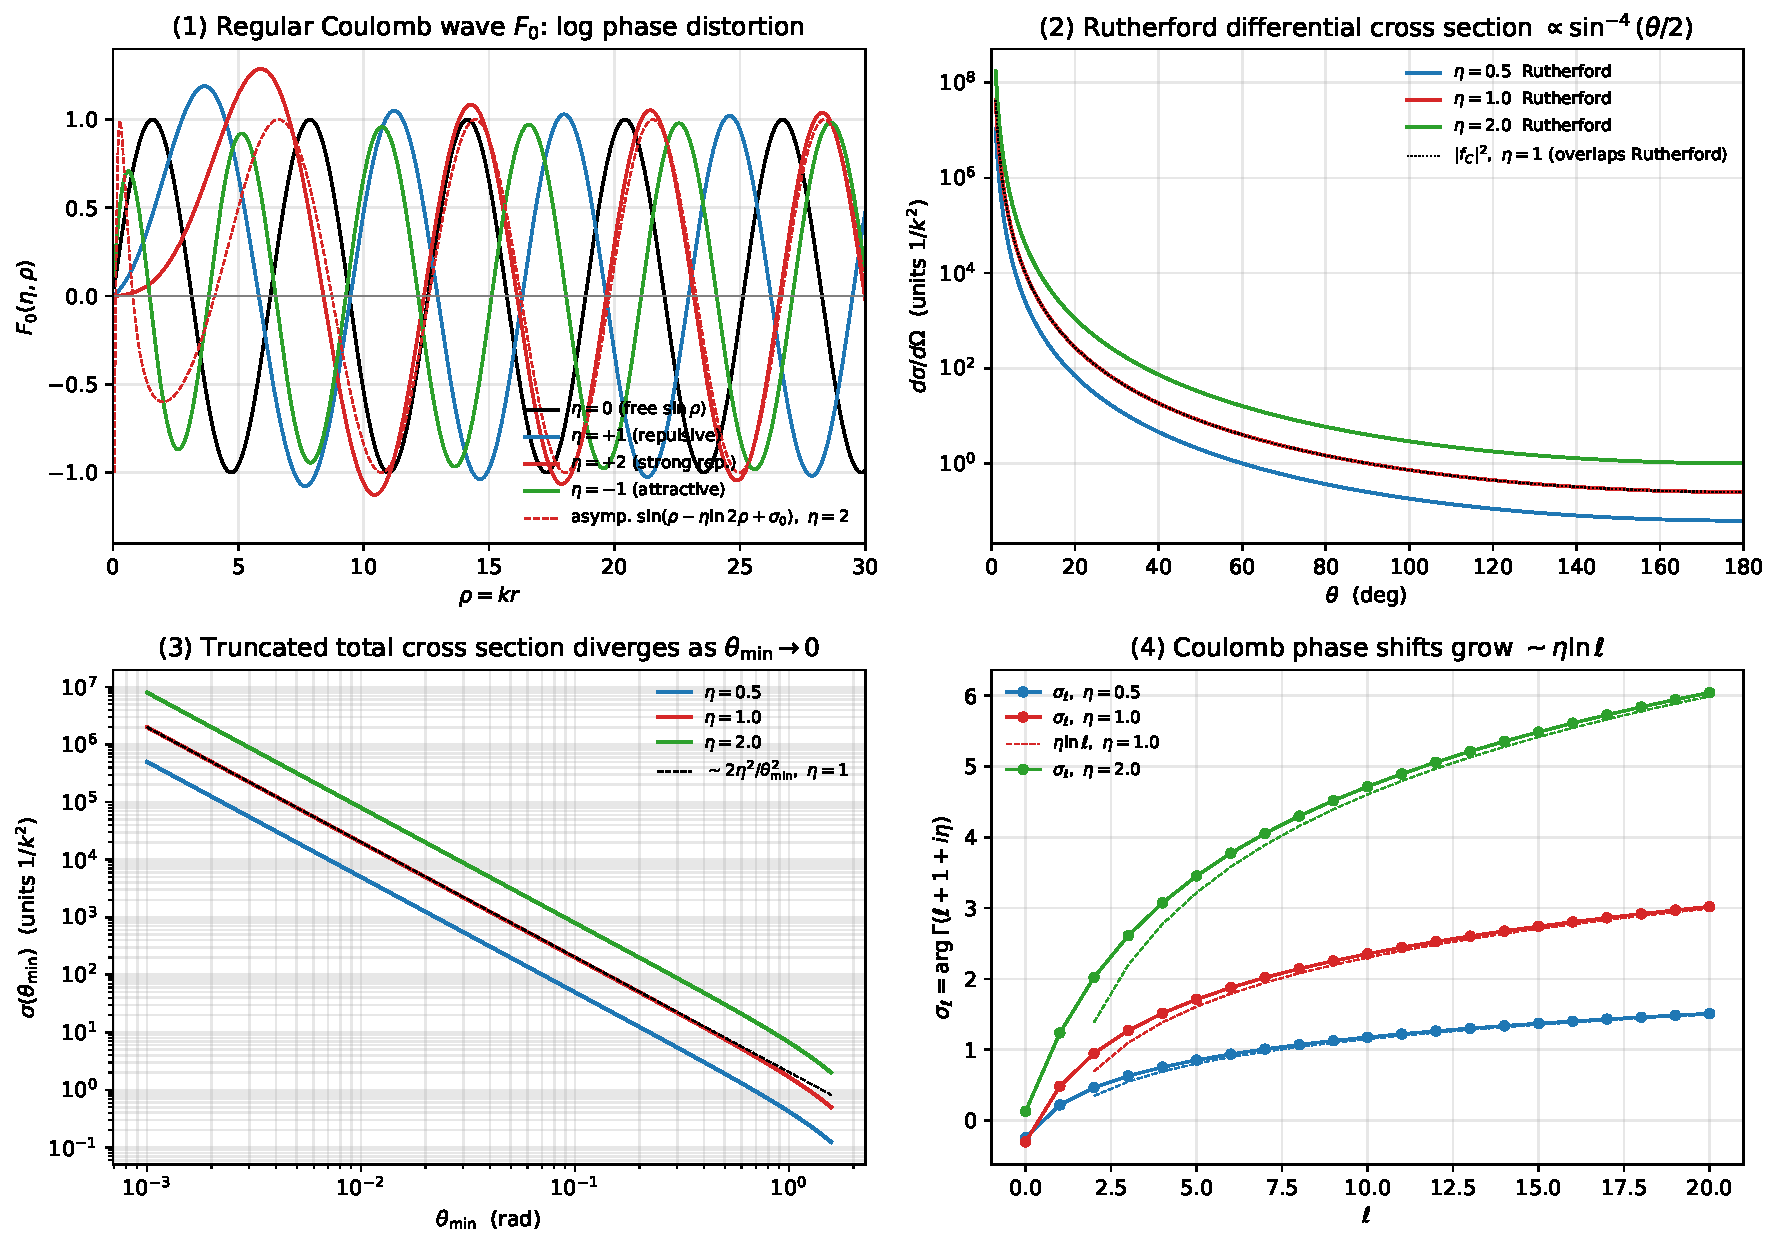
\includegraphics[width=0.95\linewidth]{ch12_coulomb}
    \caption{Coulomb 散射的四组数值验证。
      (1) 正则 Coulomb 函数 $F_0(\eta,\rho)$ 与自由 $\sin\rho$ ($\eta=0$)
      的对比：$\eta>0$ 排斥情形相位在每个周期向外推（节点远离原点），
      $\eta<0$ 吸引情形相位被往内拽；$\eta=2$ 红色虚线即渐近形式
      $\sin(\rho-\eta\ln 2\rho+\sigma_0)$，与精确 $F_0$ 在大 $\rho$ 处吻合。
      (2) 三组 $\eta$ 的 Rutherford 微分截面 $\eta^2/[4k^2\sin^4(\theta/2)]$
      （log 标度）；黑色点线 $|f_C|^2$ 与解析 Rutherford 完全重合，证实
      \eqref{eq:coulomb-fC} 的对数相位不进入 $|\cdot|^2$。
      (3) 截断总截面 $\sigma(\theta_{\min})$ 双对数图，三条线斜率 $-2$，
      与渐近 $4\pi\eta^2/\theta_{\min}^2$（黑色虚线）一致：
      $\theta_{\min}\to 0$ 时 $\sigma\to\infty$，反映 Coulomb 长程性。
      (4) Coulomb 相移 $\sigma_\ell=\arg\Gamma(\ell+1+\rmi\eta)$ 对
      $\eta=0.5,1,2$；虚线 $\eta\ln\ell$ 给出大 $\ell$ 渐近。
      可见所有 $\ell$ 上 $\sigma_\ell\ne 0$ 且不衰减。}
    \label{fig:numexp-ch12}
\end{figure}

\subsection*{物理讨论}

数值结果直接印证了本章三个核心论断。

\paragraph{对数相位畸变是真实的、不可消除的。}
图~\ref{fig:numexp-ch12}(1) 中 $\eta\ne 0$ 的 $F_0$ 与 $\eta=0$ 的
自由解 $\sin\rho$ 在大 $\rho$ 处节点位置渐行渐远 —— 这正是
$-\eta\ln 2\rho$ 项的几何体现：节点条件
$kr-\eta\ln 2kr+\sigma_0=n\pi$ 给出 $r_n\approx (n\pi-\sigma_0+\eta\ln 2kr_n)/k$，
节点间距随 $r$ 缓慢漂移。这种漂移\emph{不能}通过把对数项归入相移来消除
（\S\ref{sec:coulomb-partial} 已论证），因为它依赖 $r$；这就是为什么
``Coulomb 相移''必须把 $-\eta\ln 2kr$ 显式扣除后只取常数部分
$\sigma_\ell$ 来定义。

\paragraph{Rutherford 公式的``奇迹''。}
图~\ref{fig:numexp-ch12}(2) 说明：尽管振幅 $f_C(\theta)$ 带着复杂的
对数相位 $-\rmi\eta\ln\sin^2(\theta/2)$ 与常数 $\rme^{2\rmi\sigma_0}$
（这些相位的存在使 $f_C$ 本身依赖屏蔽方式），但模方 $|f_C|^2$
化简为纯 $\sin^{-4}(\theta/2)$ —— 这是 \S\ref{sec:coulomb-Rutherford}
所指出的``三层级巧合''（经典、Born、精确）的算术验证。换言之：
角分布是 Coulomb 散射唯一干净的可观测量，而振幅本身不是。

\paragraph{总截面发散与长程性。}
图~\ref{fig:numexp-ch12}(3) 的双对数线性行为 $\sigma\sim 1/\theta_{\min}^2$
直接对应于经典 Rutherford $\theta\sim\eta/(kb)$ 给出的关系
$\theta_{\min}\to 0\Leftrightarrow b_{\max}\to\infty$：任意大碰撞参数
$b$ 处粒子仍受偏转，故``有效散射面积''发散。这是 Coulomb 与短程力
最直观的差异：短程势的总截面有限（光学定理给出 $\sigma_{\mathrm{tot}}=
(4\pi/k)\Im f(0)$ 是有限数），而 Coulomb 的 $f_C(0)$ 本身就发散。

\paragraph{$\sigma_\ell$ 不衰减与分波级数发散。}
图~\ref{fig:numexp-ch12}(4) 中 $\sigma_\ell$ 随 $\ell$ 单调增长且
$\sim\eta\ln\ell$，这立刻暗示分波展开
$f_C=(2\rmi k)^{-1}\sum(2\ell+1)(\rme^{2\rmi\sigma_\ell}-1)P_\ell$
中的``因子''$\rme^{2\rmi\sigma_\ell}-1$ 不衰减，故级数
\emph{不绝对收敛}（与短程势分波相移 $\delta_\ell\to 0$ 形成鲜明对比，
那里级数收敛甚至指数快）。这一现象是 \S\ref{sec:coulomb-partial}
``分波展开仅在 Abel 求和意义下重现 $f_C$'' 的根本原因，并预示着
当短程力叠加于 Coulomb 之上时（\eqref{eq:coulomb-fN}），只有
``Coulomb 修正后的剩余相移'' $\delta_\ell^N$ 才会随 $\ell$ 衰减并
给出收敛的 $f_N$。

\paragraph{从数值实验到物理实践。}
本节四张图给出了把 Coulomb 长程性``可视化''的最简方案。在实际数据
分析中（如低能 $p$-$p$、$d$-$\alpha$ 散射），人们观察到的不是裸
Rutherford 而是 \eqref{eq:coulomb-sigma-cross}：Rutherford + 核相移项
+ Coulomb-核子干涉项，干涉项的振荡相位正比于
$\delta_\ell^N-\eta\ln\sin^2(\theta/2)$。本节程序提供的工具
(\texttt{coulomb\_F}, \texttt{sigma\_ell}) 也是分析此类实验数据的基础。

% ===== END CHAPTER =====
                     % Coulomb scattering
\chapter{S 矩阵的解析性质 (Analytic Properties of the S-matrix)}\label{ch:analytic}

前面几章我们已经在物理动量 $p\geq 0$ 的范围内建立了分波分析的完整框架：
正则解 (regular solution) $\phi_{l,p}(r)$、Jost 解 $\chi^\pm_{l,p}(r)$、
Jost 函数 $f_l(p)$ 以及分波 S 矩阵元 $\Smat_l(p)$。本章的核心目标是把这些函数
解析延拓到复 $p$ 平面上，研究其解析结构 (analyticity, branch cuts, poles)。
S 矩阵的解析性质是散射理论中最重要的结构性质之一：它把束缚态、共振态、阈值
行为等不同物理现象统一在同一个复平面图像中。例如，束缚态对应于 Jost 函数在
正虚轴上的零点 ($p = \rmi\kappa$)，等价地对应分波振幅的极点；准束缚 (virtual)
态出现在负虚轴；共振对应于第二 Riemann 叶上的极点；Levinson 定理则把零能与
高能相移之差直接和束缚态数目联系起来。

本章主要参考 Taylor《Scattering Theory》第 12 章，并按 Xiao 讲义的脉络组织：
(i) 单变量解析函数的若干常用工具；(ii) 正则解关于 $p$ 的整函数性质；
(iii) Jost 函数与 S 矩阵元的解析延拓区域；(iv) 束缚态与 Levinson 定理；
(v) 阈值 $p=0$ 附近的展开 (有效力程展开 / Effective range expansion)。

%======================================================================
\section{单变量解析函数的若干工具}\label{sec:analytic-tools}

我们先列出本章反复使用的复分析工具，作为参考。设 $f(z)$ 是定义在复平面上某
区域 $R$ 内的复函数。

\begin{definition}[解析函数]
$f(z)$ 在区域 $R$ 上\textbf{解析} (analytic, holomorphic)，当且仅当 $f$ 在 $R$
的任意一点都复可微。等价地，$f$ 在 $R$ 内任一点的某个邻域内可以展开为收敛的
Taylor 级数。
\end{definition}

\begin{theorem}[Cauchy 定理与公式]
若 $f$ 在单连通区域 $R$ 内解析，$\gamma\subset R$ 是一条光滑闭曲线，则
\begin{equation}
\oint_\gamma \rmd s\, f(s) = 0,\qquad
f(z) = \frac{1}{2\pi\rmi}\oint_\gamma \frac{f(s)}{s-z}\,\rmd s,
\quad z\text{ 在 }\gamma\text{ 内部}.
\label{eq:cauchy}
\end{equation}
解析函数无穷次可微，且若 $f$ 在 $R$ 中除有限多个极点外解析，则
$\dfrac{1}{2\pi\rmi}\oint \rmd z\, f(z) = \sum_{j} \Res_{z=z_j} f$ (留数定理)。
\end{theorem}

\begin{theorem}[解析延拓的唯一性]
若 $f_1(z)$ 在某条曲线 $\Gamma$ 上有定义，$f_2(z)$ 在包含 $\Gamma$ 的区域 $R$
内解析，且在 $\Gamma$ 上 $f_1=f_2$，则 $f_2$ 是 $f_1$ 由 $\Gamma$ 进入 $R$
的\emph{唯一}解析延拓。
\end{theorem}

\begin{remark}[复共轭与 Schwartz 反射原理]\label{rem:schwartz}
若 $f(z)$ 在 $R$ 内解析，则 $f^*(z)$ 一般\emph{不}在 $R^*=\{z^*:z\in R\}$ 上
解析，但 $[f(z^*)]^*$ 在 $R^*$ 内解析。\textbf{Schwartz 反射原理}：若 $R$ 包含
实轴上的一段，$f$ 在 $R$ 内解析，且当 $z$ 在该段实轴上时 $f(z)\in\R$，则
\begin{equation}
f^*(z) = f(z^*),\qquad z\in R\cup R^*.
\label{eq:schwartz}
\end{equation}
\end{remark}

下面两个定理是把级数展开和参数积分提升为 "解析" 的关键判据。

\begin{theorem}[级数与积分给出的解析函数]\label{thm:series-integral}
\hfill
\begin{enumerate}
\item\emph{(级数求和)}\; 设 $f_n(z)$ 在区域 $R$ 上解析，且级数
$\sum_n f_n(z)$ 在 $R$ 上一致收敛，则 $f(z)=\sum_n f_n(z)$ 在 $R$ 上解析。
\item\emph{(参数积分)}\; 设对每一 $r\in(a,b)\subset\R$，函数 $g(z,r)$ 在 $R$
上解析，且 $g$ 在 $R\times(a,b)$ 上连续，则
$f(z)=\int_a^b\rmd r\,g(z,r)$ 在 $R$ 上解析。
\end{enumerate}
\end{theorem}

\begin{remark}\label{rem:improper}
第二条可以推广到反常积分：当 $a=0$ 时 $g(z,0)$ 发散、或 $b=\infty$、或者
存在某 $r_0$ 处 $g(z,r_0)$ 发散，只要在端点 (与可疑点) 处积分关于 $z$
\emph{一致收敛}，结论仍然成立。这是后面证明 Jost 函数解析性的核心工具。
\end{remark}

%======================================================================
\section{正则解的解析性质}\label{sec:regular-analytic}

考虑约化 Schr\"odinger 径向方程 (取 $2m=1$，势 $U=2mV$)
\begin{equation}
\left[\frac{\rmd^2}{\rmd r^2}-\frac{l(l+1)}{r^2}+p^2-U(r)\right]\psi_l(r)=0.
\label{eq:radial}
\end{equation}
\textbf{正则解} $\phi_{l,p}(r)$ 由 $r\to0$ 处的边界条件
$\phi_{l,p}(r)\sim \hat{j}_l(pr)$ 唯一确定 (其中 $\hat{j}_l(x)=xj_l(x)$，
$\hat{j}_l(x)\to x^{l+1}/(2l+1)!!$ 当 $x\to 0$)。它满足等价的 Volterra
积分方程
\begin{equation}
\phi_{l,p}(r)=\hat{j}_l(pr)+\lambda\int_0^r \rmd r'\,g_{l,p}(r,r')\,U(r')\,\phi_{l,p}(r'),
\label{eq:phi-volterra}
\end{equation}
其中 Green 核为
\begin{equation}
g_{l,p}(r,r')=\frac{1}{p}\bigl[\hat j_l(pr)\hat n_l(pr')-\hat n_l(pr)\hat j_l(pr')\bigr].
\label{eq:greenkernel}
\end{equation}
注意 $\hat j_l, \hat n_l$ 当 $z\to 0$ 分别行为为 $z^{l+1}, z^{-l}$，因此 $g_{l,p}(r,r')$
作为 $p$ 的函数是\emph{整函数} (entire)。

\begin{theorem}[正则解关于 $p$ 是整函数]\label{thm:phi-entire}
对于任意 $p\in\C$ (实或复)，由迭代级数定义的 \eqref{eq:phi-volterra} 解
$\phi_{l,p}(r)$ 关于 $p$ 在整个复平面上解析 (即 $p$ 的整函数)。
\end{theorem}

\begin{proof*}
由 Neumann 迭代展开
\begin{equation}
\phi_{l,p}(r)=\hat j_l(pr)+\sum_{n=1}^\infty \lambda^n\,\phi^{(n)}(r),\qquad
\phi^{(n)}(r)=\frac{1}{p^n}\!\!\int_0^r\!\!\rmd r_n\!\int_0^{r_n}\!\!\rmd r_{n-1}\cdots
\!\int_0^{r_2}\!\!\rmd r_1\,
g_{l,p}(r,r_n)U(r_n)\cdots g_{l,p}(r_2,r_1)U(r_1)\hat j_l(pr_1).
\label{eq:phi-iter}
\end{equation}
对 $l=0$ 分波，$g_{0,p}(r,r')=\sin p(r-r')/p$。利用经典估计
$|\sin z|\leq \beta\,|z|/(1+|z|)\,\rme^{|\Im z|}$ ($\beta$ 是数值常数)，得到
\begin{equation}
|\phi^{(n)}(r)|\leq \beta\,\frac{|pr|}{1+|pr|}\,\rme^{|\Im p|r}\,\frac{\alpha^n}{n!},\qquad
\alpha\equiv\int_0^r\rmd r'\,|U(r')|\,r'.
\label{eq:phi-bound-l0}
\end{equation}
对一般 $l$，类似的估计给出
\begin{equation}
|\phi_{l,p}(r)|\leq \gamma_l\,\Bigl(\frac{|pr|}{1+|pr|}\Bigr)^{l+1}\,\rme^{|\Im p|r},
\label{eq:phi-bound-general}
\end{equation}
其中 $\gamma_l$ 是只依赖于 $l$ 的常数。在 $p$ 的任意有界区域内，$|\phi^{(n)}|$
有共同的可求和上界，故 \eqref{eq:phi-iter} 关于 $p$ 一致收敛；又每一项
$\phi^{(n)}(r)$ 是 $p$ 的整函数 (由定理 \ref{thm:series-integral} 与
注 \ref{rem:improper})，故和也是 $p$ 的整函数。
\end{proof*}

\eqref{eq:phi-bound-general} 同时给出了正则解在大 $|p|$ 下的指数控制：
$|pr|^{l+1}/(1+|pr|)^{l+1}$ 反映了 $\hat j_l(pr)\sim (pr)^{l+1}$ 当 $pr\to 0$
的低能行为，而因子 $\rme^{|\Im p|r}$ 反映了 $\hat j_l(z)\sim\sin(z-l\pi/2)$
当 $|\Im z|\to\infty$ 的高能行为。

\begin{remark}[$p\to-p$ 的对称性]\label{rem:phi-parity}
由 $\hat j_l(-z)=(-1)^{l+1}\hat j_l(z)$，$\hat n_l(-z)=(-1)^l\hat n_l(z)$，可得
$g_{l,-p}(r,r')=g_{l,p}(r,r')$。对积分方程 \eqref{eq:phi-volterra} 两边比较
$p\to -p$ 即得
\begin{equation}
\phi_{l,-p}(r)=(-1)^{l+1}\phi_{l,p}(r).
\label{eq:phi-parity}
\end{equation}
也即 $\phi_{l,p}$ 是 $p$ 的奇 (或偶) 函数，依 $l$ 而定。
\end{remark}

\textbf{两种诠释}\quad 上述结果有两种等价的物理诠释：
\begin{itemize}
\item $\phi_{l,p}(r)$ 是 \eqref{eq:phi-volterra} (复 $p$ 的方程) 的解，关于 $p$
解析，回到物理区域 $p\geq 0$ 时退回物理解；
\item $\phi_{l,p}(r)$ 由物理区域 $p\geq 0$ 上的解析延拓给出复 $p$ 的解。
\end{itemize}
两种观点结合定理 \ref{thm:phi-entire} 给出同一个 $p$ 整函数。

%======================================================================
\section{Jost 函数与分波 S 矩阵元的解析性}\label{sec:jost-analytic}

回顾 Jost 函数的定义：在 $r\to\infty$ 处把正则解写成入射 + 出射球面波的
线性组合
\begin{equation}
\phi_{l,p}(r)\xrightarrow{r\to\infty}
\frac{\rmi}{2}\Bigl[f_l(p)\,\hat h^-_l(pr)-f_l(-p)\,\hat h^+_l(pr)\Bigr],
\label{eq:phi-asymp}
\end{equation}
其中 $\hat h^\pm_l(z)\to (\mp\rmi)^{l+1}\rme^{\pm\rmi z}$ 当 $|z|\to\infty$。
等价地用 Jost 解 $\chi^\pm_{l,p}(r)$ (满足 $\chi^\pm_{l,p}(r)\to\hat h^\pm_l(pr)$)
通过 Wronskian 表达
\begin{equation}
f_l(p)=\frac{1}{p}\,W(\chi^+_{l,p},\phi_{l,p}),\qquad
W(\alpha,\beta)\equiv \alpha\beta'-\alpha'\beta.
\label{eq:fW}
\end{equation}
作为公式更方便的，是积分表达
\begin{equation}
f_l(p)=1+\frac{\lambda}{p}\int_0^\infty \rmd r'\,\hat h^+_l(pr')\,U(r')\,\phi_{l,p}(r').
\label{eq:fl-int-ch11}
\end{equation}
这个式子定义了 $f_l(p)$ 到复 $p$ 平面的解析延拓 (只要积分收敛即可)。

%--------------------------------------------------------------------
\subsection{上半平面的解析性}\label{ssec:upper}

复 $p$ 时，根据 \eqref{eq:phi-bound-general} 与
$|\hat h^+_l(pr)|\leq (\beta|pr|/(1+|pr|))^{-l}\,\rme^{-\Im p\, r}$，
被积函数受控于
\begin{equation}
|\hat h^+_l(pr')\,U(r')\,\phi_{l,p}(r')|
\leq \mathrm{const}\cdot \frac{\beta\,|p|\,r'}{1+|pr'|}\,|U(r')|\,
\rme^{(|\Im p|-\Im p)r'}.
\label{eq:integrand-bound}
\end{equation}
若 $\Im p>0$，则指数因子 $\rme^{(|\Im p|-\Im p)r'}=1$，积分关于 $r'$ 一致收敛
(只要 $r|U(r)|\in L^1$)，由定理 \ref{thm:series-integral} 与
注 \ref{rem:improper}，
\begin{equation}
\boxed{\;f_l(p)\text{ 在上半平面 }\Im p\geq 0\text{ 内解析。}\;}
\label{eq:fl-upper}
\end{equation}

\begin{remark}[势的形态决定下半平面行为]\label{rem:potential-tail}
下半平面的解析性依赖于势的具体长程行为：
\begin{itemize}
\item \textbf{截断势}\,： $r>a$ 时 $U(r)=0$，则 \eqref{eq:fl-int-ch11} 的积分上限
变为 $a$，对所有 $p\in\C$ 收敛，故 $f_l(p)$ 在\emph{整个复平面}上解析
(即 $f_l$ 是整函数)。
\item \textbf{Yukawa 型势} $V\sim \rme^{-\mu r}$\,： \eqref{eq:integrand-bound}
要求 $|\Im p|-\Im p+\mu>0$，即 $\Im p>-\mu/2$，故 $f_l(p)$ 在
$\Im p>-\mu/2$ 解析。
\item 一般 $\rme^{-\mu r}/r$ 型 (Yukawa)\,： $f_l$ 在负虚轴 $p=-\rmi\mu/2,
-\rmi\mu,\ldots$ 处可能有支点 (branch cut)；若 $V\sim\gamma\rme^{-\mu r}$
(非 Yukawa) 则在这些点是\emph{极点}。
\end{itemize}
\end{remark}

%--------------------------------------------------------------------
\subsection{解析势与解析延拓的扩张}\label{ssec:analytic-potential}

若势 $V(r)$ 本身在 $\Re r>0$ 半平面上解析，且对从原点出发的射线 $r=\rho\rme^{\rmi\theta}$
($|\theta|<\pi/2$) 仍有相同的衰减性质，则称之为\textbf{解析势} (analytic
potential)。此时 \eqref{eq:fl-int-ch11} 的 $r$ 积分路径可以变形到复平面上沿射线
$r=\rho\rme^{\rmi\theta}$ 进行：
\begin{equation}
f_l(p)=1+\frac{1}{p}\int_0^{\infty\rme^{\rmi\theta}}\rmd r\,\hat h^+_l(pr)\,U(r)\,\phi_{l,p}(r).
\label{eq:fl-rotated}
\end{equation}
被积函数仍由 \eqref{eq:phi-bound-general} 控制：估计中
$\rme^{|\Im p|r}\to\rme^{|\Im(p\rme^{\rmi\theta})|\rho}$，
$\rme^{-\Im p\,r}\to\rme^{-\Im(p\rme^{\rmi\theta})\rho}$，故关键条件变为
$\Im(p\rme^{\rmi\theta})\geq 0$，即 $p$ 落在以 $-\theta$ 为转角的旋转半平面内。
让 $\theta$ 取遍 $(-\pi/2,\pi/2)$，所有这些半平面的并集是
$\C\setminus(-\rmi\R_+)$ —— 即整个复平面上扣除负虚轴。

\begin{theorem}[解析势的 $f_l$ 解析延拓]
若势 $U(r)$ 在右半平面 $\Re r>0$ 上解析，并对所有从原点出发的射线
$r=\rho\rme^{\rmi\theta}$ 满足前述衰减条件，则 $f_l(p)$ 解析延拓到\emph{除负虚轴
之外}的整个复 $p$ 平面 (Taylor 教材图 12.5)。
\end{theorem}

如果只要求 $V$ 在 $r>a$ 处解析 (而非 $\Re r>0$ 全域)，可选择从 $r=a$ 处弯折
进入复 $r$ 平面的积分路径，结论仍然成立。

\begin{remark}[Yukawa 型势的支割线]
若势同时是解析势 (例如 $V\sim\gamma\rme^{-\mu r}/r$ 是经典 Yukawa)，结合上面两种
情形，$f_l(p)$ 在负虚轴 $p=-\rmi\mu/2,-\rmi\mu,\ldots$ 上有\emph{割线}，
而对纯指数 $V\sim\gamma\rme^{-\mu r}$ 则是\emph{极点}。$\Smat_l(p)$ 在以下
区域内亚纯：
\begin{equation}
-\mu/2<\Im p<\mu/2.
\label{eq:Sl-meromorphic}
\end{equation}
\end{remark}

\begin{remark}[关于下半平面解析性的两点说明]\label{rem:two-remarks}
\begin{enumerate}
\item 对于满足 "上半平面解析" 这种较弱要求的势，要把 $f_l(p)$ 解析延拓到下半
平面需要额外的条件 (例如解析势 / 截断势 / Yukawa)。
\item 物理上 $f_l(p)$ 在下半平面的解析性\emph{并不重要}，下半平面 (尤其负虚轴)
的细节对势的长程行为非常敏感。例如 $\rme^{-\mu r}/r$ 在负虚轴有割线，但若
在 $r>a$ 处截断 ($a$ 很大)，则变成整函数。两种势在物理上不可区分，但解析
结构差别很大。
\end{enumerate}
\end{remark}

%--------------------------------------------------------------------
\subsection{$p\to-p$ 与复共轭对称}\label{ssec:symmetries}

由 $\phi_{l,-p}(r)=(-1)^{l+1}\phi_{l,p}(r)$ 和 $\hat h^+_l(-z)=(-1)^{l+1}\hat h^{+*}_l(z)$
(对实 $z$)，把 $p\to-p$ 代入 \eqref{eq:fl-int-ch11}，对实 $p$ 立刻得到
\begin{equation}
f_l(-p) = [f_l(p)]^*,\qquad p\in\R.
\label{eq:fl-real-conj}
\end{equation}
两边都是 $p$ 的解析函数 (在合适区域内)，由唯一性可解析延拓为
\begin{equation}
\boxed{\;f_l(-p) = [f_l(p^*)]^*,\qquad p\in\C.\;}
\label{eq:fl-schwartz}
\end{equation}
这是 Schwartz 反射原理的直接体现。若 $p$ 在虚轴上 (即 $p^*=-p$)，则
$f_l(-p)=[f_l(-p)]^*$，即 $f_l$ 在虚轴上取实值；$f_l(p)$ 关于虚轴对称两点
互为复共轭。

由 $\Smat_l(p)=f_l(-p)/f_l(p)$ 立得
\begin{equation}
\Smat_l(p)\xrightarrow{p\in\R}\frac{[f_l(p)]^*}{f_l(p)},\qquad
\Smat_l(p)\xrightarrow{p\in\C}\frac{[f_l(p^*)]^*}{f_l(p)}=\frac{f_l(-p)}{f_l(p)}.
\label{eq:Sl-from-fl}
\end{equation}
后两个表达式中，分母关于 $\Im p\geq 0$ 解析，分子关于 $\Im p\leq 0$ 解析。
对于实 $p$ 进而得到\textbf{幺正性恒等式}
\begin{equation}
\Smat_l(p)\,\Smat_l(-p)=\frac{f_l(-p)}{f_l(p)}\cdot\frac{f_l(p)}{f_l(-p)}=1,\qquad
|\Smat_l(p)|^2 = 1.
\label{eq:unitarity}
\end{equation}

%======================================================================
\section{Riemann 面上的 S 矩阵：$E$ 平面图像}\label{sec:riemann}

物理能量与动量的关系是 $E=p^2/(2m)$ (取 $2m=1$ 时 $E=p^2$)。从 $p$ 平面到
$E$ 平面的映射是 2 对 1 的：$\pm p$ 对应同一个 $E$。因此在 $E$ 平面上
$\Smat_l$ 一般是 \emph{Riemann 双叶面} 上的函数：

\begin{itemize}
\item \textbf{物理叶 (physical sheet)}\,：对应 $p$ 平面的上半 $\Im p>0$，
覆盖 $E$ 平面剪开沿正实轴 ($E\geq 0$, 散射阈值之上) 的区域；正能 $E>0$
对应 $p\in\R_+$。
\item \textbf{第二叶 (second / unphysical sheet)}\,：对应 $\Im p<0$，
通过把 $E$ 平面割线上下唇粘合得到。
\end{itemize}

物理叶上 (上半 $p$ 平面)，$\Smat_l$ 在束缚态对应的正虚轴点
$p=\rmi\kappa_n$ 处有极点 (实际上是 $f_l(p)$ 的零点)；负实能 $E_n=-\kappa_n^2/(2m)<0$。
第二叶上 (下半 $p$ 平面) 的极点 $p=p_R-\rmi\Gamma/2$ 对应共振，$E_R=p_R^2-\rmi p_R\Gamma$
位于实轴下方。\emph{虚态}\, (virtual / antibound state) 是负虚轴上的零点
$p=-\rmi\kappa$，对应负 $E$，但在第二叶上而非物理叶。

%======================================================================
\section{束缚态与 Levinson 定理}\label{sec:bound-states}

%--------------------------------------------------------------------
\subsection{束缚态对应 Jost 函数的零点}\label{ssec:bound-zeros}

回到渐近形式 \eqref{eq:phi-asymp}。当 $\Im p>0$ 时，$\hat h^+_l(pr)\to0$ 而
$\hat h^-_l(pr)\to\infty$。设在某 $\bar p$ ($\Im\bar p>0$) 处
$f_l(\bar p)=0$，则 \eqref{eq:phi-asymp} 中 "上升" 项消失，剩
\begin{equation}
\phi_{l,\bar p}(r)\xrightarrow{r\to\infty}
-\frac{\rmi}{2}f_l(-\bar p)\,\hat h^+_l(\bar p r)
\sim \rme^{\rmi(\bar p r-l\pi/2)},
\end{equation}
当 $\Im\bar p>0$ 时这是\emph{指数衰减}的，配合 $\phi_{l,\bar p}(0)=0$，
$\phi_{l,\bar p}$ 是平方可积的——恰是 Schr\"odinger 方程的束缚态波函数。

由于 $\Hmat$ 是 Hermitian 算符，束缚态本征值 $E=p^2/(2m)$ 必为实，故
$\bar p$ 必为\emph{纯虚数}：$\bar p=\rmi\kappa$ ($\kappa>0$)，$E=-\kappa^2/(2m)$。

\begin{theorem}[束缚态 $\Leftrightarrow$ Jost 函数零点]\label{thm:bound-zero}
对满足前述条件的中心势 $V(r)$，每一个角动量 $l$ 子空间内的束缚态 (本征值
$E_n=-\kappa_n^2/(2m)<0$) 与 Jost 函数 $f_l(p)$ 在正虚轴上的一阶零点
$p=\rmi\kappa_n$ 一一对应；等价地与分波 S 矩阵元 $\Smat_l(p)=f_l(-p)/f_l(p)$
在正虚轴上的一阶极点一一对应。
\end{theorem}

\begin{proof*}\!(简要)
设 $f_l(\bar p)=0$，$\Im\bar p>0$。由 Wronskian 表达 \eqref{eq:fW}，
$W(\chi^+_{l,\bar p},\phi_{l,\bar p})=0$，故 $\chi^+_{l,\bar p}$ 与
$\phi_{l,\bar p}$ 线性相关：$\phi_{l,\bar p}(r)=\lambda\,\chi^+_{l,\bar p}(r)$。
$\chi^+_{l,\bar p}(r)\to\hat h^+_l(\bar p r)$ 指数衰减，故 $\phi_{l,\bar p}$
平方可积且满足 Schr\"odinger 方程，$E=\bar p^2/(2m)$ 是束缚态能量。反过来
若有束缚态，则同样的 $\phi_{l,\bar p}\propto\chi^+_{l,\bar p}$ 关系成立，
推出 $f_l(\bar p)=0$。

\textbf{零点为单阶}：考虑 $\rmd f_l/\rmd p$。利用 \eqref{eq:fl-int-ch11} 的等价积分
表达 (经辐向方程的 Wronskian 操作可化为)
\begin{equation}
\frac{\rmd f_l}{\rmd p}(\bar p)=\int_0^\infty \rmd r\,\chi^+_{l,\bar p}(r)\,\phi_{l,\bar p}(r)
=\lambda\int_0^\infty \rmd r\,[\chi^+_{l,\bar p}(r)]^2\neq 0,
\end{equation}
因为束缚态波函数本身归一化非零。详见 Taylor 习题 12.3。
\end{proof*}

\begin{remark}[分波振幅的留数]
分波振幅 $f_l^{\text{amp}}(p)=[\Smat_l(p)-1]/(2\rmi p)$ 在 $\bar p=\rmi\kappa_n$
处是一阶极点，留数为
\begin{equation}
\Res_{p=\rmi\kappa_n}\Smat_l(p) = \frac{f_l(-\rmi\kappa_n)}{(\rmd f_l/\rmd p)|_{\rmi\kappa_n}}.
\end{equation}
对 $E$ 平面：分波振幅在 $E_n=-\kappa_n^2/(2m)$ 处的留数为
$\Gamma_n=(-1)^{l+1}\gamma_n^2/(2m)$，其中 $\gamma_n$ 是归一化束缚态径向波函数
在 $r\to\infty$ 处的渐近形式 $\eta(r)\to\gamma_n\rme^{-\kappa_n r}$ 中的常数
(见 Taylor 习题 12.3)。
\end{remark}

%--------------------------------------------------------------------
\subsection{Levinson 定理}\label{ssec:levinson}

\begin{theorem}[Jost 函数关于 $p$ 的两个性质]\label{thm:fl-properties}
\hfill
\begin{enumerate}
\item $f_l(p)$ 在实轴上 (除可能 $p=0$ 外) 不能取零值；
\item 当 $|p|\to\infty$ 且 $\Im p\geq 0$ 时，$f_l(p)\to 1$，更精确地
\begin{equation}
f_l(p)-1 = O(|p|^{-\eta}),\qquad |p|\to\infty,\ \Im p\geq 0,
\label{eq:fl-large}
\end{equation}
均匀地对某 $\eta>0$ 成立。
\end{enumerate}
\end{theorem}

\begin{proof*}
1) 若实 $p\neq 0$ 满足 $f_l(p)=0$，则也有 $f_l^*(p)=f_l(-p)=0$。
渐近式 \eqref{eq:phi-asymp} 的两个 "Hankel" 项同时消失，结合
$r\to 0$ 处 $\phi_{l,p}(r)\to (pr)^{l+1}/(2l+1)!!\neq 0$ (除非 $p=0$)，
得 $\phi_{l,p}\equiv 0$，矛盾。

2) 由 \eqref{eq:fl-int-ch11} 估计被积函数即得；详见上一章关于 Jost 函数大 $p$
渐近的讨论的复 $p$ 推广。
\end{proof*}

\begin{corollary}[束缚态有限性]\label{cor:bound-finite}
对固定的 $l$，$f_l(p)$ 在上半平面 $\Im p>0$ 中只有\emph{有限个}零点，即只有
有限个束缚态。 ($p=0$ 处需特殊考虑，见 \S\ref{sec:threshold}。)
\end{corollary}

\begin{proof*}
由性质 2，存在 $p_0>0$ 使得 $|p|>p_0$ 时 $f_l(p)\neq 0$；上半平面内 $|p|\leq p_0$
是有界闭区域，解析函数在有界闭区域上不能有无穷多孤立零点。
\end{proof*}

\begin{theorem}[Levinson 定理]\label{thm:levinson}
对球对称势 $V(r)$ (满足前面的衰减条件)，分波 $l$ 的相移 $\delta_l(p)$ 满足
\begin{equation}
\boxed{\;\delta_l(0)-\delta_l(\infty) = n_l\,\pi\;}
\label{eq:levinson}
\end{equation}
其中 $n_l$ 是分波 $l$ 中的束缚态个数。例外情形：当 $l=0$ 且 $f_0(0)=0$ 时
("零能 s 波束缚态")，则
\begin{equation}
\delta_0(0)-\delta_0(\infty) = (n_0+\tfrac{1}{2})\pi.
\label{eq:levinson-exc}
\end{equation}
\end{theorem}

\begin{proof*}\!(主要思想，$f_l(0)\neq 0$ 情形)
考察上半平面的辐角原理积分
\begin{equation}
I=\oint \rmd\ln f_l(p) = \oint \rmd p\,\frac{f_l'(p)}{f_l(p)} = 2\pi\rmi\,n_l,
\label{eq:argprinciple}
\end{equation}
其中环路取 "大半圆"：实轴 $p\in[-R,R]$ 加 $|p|=R$ 的上半圆 (取 $R\to\infty$)。

(i) 实轴上 ($p>0$)，由 $|f_l|^2$ 在分波幺正性下与相移的关系
$f_l(p)=|f_l(p)|\rme^{-\rmi\delta_l(p)}$，并利用 $f_l(-p)=f_l^*(p)$ 反演到 $p<0$
段。综合两段实轴贡献：
\begin{equation}
I_{\text{real}}=\int_{-\infty}^\infty\rmd\ln f_l(p) = -2\rmi\int_0^\infty\rmd\delta_l(p)
=-2\rmi[\delta_l(\infty)-\delta_l(0)].
\end{equation}
(ii) 大半圆 $|p|=R\to\infty$ 上，$f_l\to 1$，故 $\rmd\ln f_l\to 0$，圆上贡献
为零。

合起来 $-2\rmi[\delta_l(\infty)-\delta_l(0)]=2\pi\rmi n_l$，即
$\delta_l(0)-\delta_l(\infty)=n_l\pi$。
\end{proof*}

\begin{remark}[$f_l(0)=0$ 例外情形]
若 $l=0$ 且 $f_0(0)=0$ (即在阈值 $p=0$ 处恰有一个 "零能束缚态"，物理上对应散射
长度发散)，则环路在 $p=0$ 处需绕一个小半圆 $\Gamma_\epsilon$。该小半圆贡献
$-\pi\rmi$ ($l=0$ 时 $f_0(p)\sim\rmi\gamma p$，$\rmd\ln f_0/\rmd p\sim 1/p$)
或 $-2\pi\rmi$ ($l>0$ 时 $f_l(p)\sim\beta p^2$，零点为二阶根)。详细计算见
\S\ref{ssec:threshold-zero}。
\end{remark}

%======================================================================
\section{阈值 $p=0$ 附近的行为}\label{sec:threshold}

阈值是物理动量与解析延拓的交界，散射截面的低能行为由 $p=0$ 处
$f_l(p),\Smat_l(p)$ 的展开主导。

%--------------------------------------------------------------------
\subsection{$f_l(0)\neq 0$ 时的展开}\label{ssec:threshold-nonzero}

分波振幅可写为
\begin{equation}
f_l^{\text{amp}}(p)=\frac{\Smat_l(p)-1}{2\rmi p}
=\frac{f_l(-p)-f_l(p)}{2\rmi p\,f_l(p)}
=-\frac{1}{p^2 f_l(p)}\int_0^\infty\rmd r\,\hat j_l(pr)\,U(r)\,\phi_{l,p}(r).
\label{eq:amp-int}
\end{equation}
利用 $|\hat j_l(pr)|,|\phi_{l,p}(r)|\leq \mathrm{const}\cdot[pr/(1+pr)]^{l+1}$，
若 $f_l(0)\neq 0$，则
\begin{equation}
|f_l^{\text{amp}}(p)|\leq \frac{\mathrm{const}}{|f_l(0)|}\,\frac{1}{|p|^2}
\int_0^\infty \rmd r\,|U(r)|\,\Bigl(\frac{|p|r}{1+|p|r}\Bigr)^{2l+2}.
\label{eq:amp-bound}
\end{equation}
对指数压低 (Yukawa 型) 的势，分母 $1+pr\to 1$ ($p\to 0$ 与 $r$ 实际范围有限
共同保证)，故 $f_l^{\text{amp}}(p)=O(p^{2l})$。等价的 Taylor 展开
\begin{equation}
\boxed{\;f_l^{\text{amp}}(p)=-a_l\,p^{2l}+b_l\,p^{2l+1}+\cdots,\qquad p\to 0\;}
\label{eq:scattering-length}
\end{equation}
其中 $a_l$ 是有限常数 (可能为零)，$l=0$ 时即为\textbf{散射长度} (scattering length)。

\begin{remark}[长程势的破坏]
当 $r\to\infty$ 时 $V(r)=O(1/r^\nu)$ ($\nu>0$，幂律 tail) 而非指数衰减时，
\eqref{eq:amp-bound} 中分母 $1+pr$ 不能直接置 $1$，需要更细致的分析：
\begin{itemize}
\item $l<(\nu-3)/2$ 时积分仍收敛，$f_l^{\text{amp}}=O(p^{2l})$；
\item $l>(\nu-3)/2$ 时积分需保留 $1+pr$ 因子，结果是 $f_l^{\text{amp}}=O(p^{\nu-3})$。
\end{itemize}
此时 $p=0$ 处的解析行为未知，不一定能展开为整次幂。例如 $1/r^4$ tail 给出
$p\cot\delta_0(p)=-1/a_0+bp+cp^2\ln p+O(p^2)$ (含对数项)。
\end{remark}

%--------------------------------------------------------------------
\subsection{有效力程展开 (Effective range expansion)}\label{ssec:effective-range}

对 $f_l(0)\neq 0$ 的情形，引入分波振幅的 \emph{K 矩阵参数化}
\begin{equation}
\Smat_l(p)=\frac{1+\rmi k_l(p)}{1-\rmi k_l(p)},\qquad
k_l(p)=\rmi\,\frac{1-\Smat_l(p)}{1+\Smat_l(p)}=\tan\delta_l(p).
\label{eq:K-matrix}
\end{equation}
对实 $p>0$，$k_l(p)$ 实，$\Smat_l$ 自动幺正。除 $\Smat_l=-1$ (此即
$\delta_l=\pi/2$，相对应 K 矩阵奇点) 外，$k_l$ 在 $\Smat_l$ 解析的点处解析，
\emph{特别地在 $p=0$ 处解析} (假设 $f_l(0)\neq 0$)。

由 $\Smat_l(-p)=1/\Smat_l(p)$ 推出 $k_l(-p)=-k_l(p)$，是 $p$ 的奇函数。结合
低能行为 $\delta_l(p)\to a_l p^{2l+1}$ 给出
\begin{equation}
k_l(p)\xrightarrow{p\to 0} -a_l\,p^{2l+1}.
\label{eq:kl-low}
\end{equation}
故 $k_l/p^{2l+1}$ 是 $p^2$ 的偶函数且在原点解析，可展开为
\begin{equation}
\boxed{\;\frac{p^{2l+1}}{k_l(p)} = p^{2l+1}\cot\delta_l(p)
= -\frac{1}{a_l}+\frac{r_l}{2}\,p^2+O(p^4)\;}
\label{eq:eff-range-ch11}
\end{equation}
这就是著名的\textbf{有效力程展开}。其中：
\begin{itemize}
\item $a_l$\,：分波 $l$ 的散射长度；
\item $r_l$\,：分波 $l$ 的有效力程 (effective range)；对 $l=0$，$r_0$ 物理近似
等于势的有效范围。
\end{itemize}
仅取前两项的近似称为\textbf{有效力程近似} (effective range approximation)。
对 $n$-$p$ 散射，能量低于 $10\,\mathrm{MeV}$ 时该近似精度很高。

\begin{remark}[$1/r^\nu$ tail 破坏 $p^2$ 展开]
对长程 $1/r^\nu$ 型势，$\Smat_l(p)$ 在 $p=0$ 一般含有支点 (例如
$1/r^4$ tail 给出 $p\cot\delta_0=-1/a_0+bp+cp^2\ln p+O(p^2)$)，无法做关于
$p^2$ 的整次幂 effective range expansion。
\end{remark}

%--------------------------------------------------------------------
\subsection{阈值零点 $f_l(0)=0$}\label{ssec:threshold-zero}

考虑特殊情形 $f_l(0)=0$。$p=0$ 时径向方程退化为
\begin{equation}
\Bigl[\frac{\rmd^2}{\rmd r^2}-\frac{l(l+1)}{r^2}-U(r)\Bigr]y(r)=0,
\end{equation}
$r\to 0,\infty$ 由 $l(l+1)/r^2$ 项主导：
\begin{itemize}
\item $r\to 0$\,： $y(r)\sim r^{l+1}$；
\item $r\to\infty$\,： 自由解 $y\sim r^{l+1}$ 与 $y\sim 1/r^l$，物理选择
$1/r^l$。
\item 对 $l=0$， $r\to\infty$，$y\sim 1/r^0=$ 常数，\emph{不可归一化}，故
\emph{不是}束缚态。
\item 对 $l>0$， $y\sim 1/r^l$ 平方可积 (在 $r\to\infty$ 端)，\emph{可以}是
束缚态 (零能束缚态)。
\end{itemize}
能否两端同时满足，依赖势的细节，只对特殊解才存在。

\textbf{$f_l(p)$ 在 $p=0$ 趋零的方式}\quad 假设势指数衰减，可以在 \eqref{eq:fl-int-ch11}
内展开 $\hat h^+_l(pr)=\hat n_l(pr)+\rmi\hat j_l(pr)$：
\begin{align}
f_l(p)&=1+\frac{1}{p}\int_0^\infty\rmd r\,\hat n_l(pr)\,U(r)\,\phi_{l,p}(r)
+\frac{\rmi}{p}\int_0^\infty\rmd r\,\hat j_l(pr)\,U(r)\,\phi_{l,p}(r)\\
&\xrightarrow{p\to 0} 1+[\alpha_l+\beta_l p^2+O(p^4)]+\rmi[\gamma_l p^{2l+1}+O(p^{2l+3})].
\label{eq:fl-zero-expand}
\end{align}
注意 $\hat j_l, \hat n_l, \phi_{l,p}$ 是实的 (对实 $p$)，故 $\alpha_l,\beta_l,\gamma_l$
都是实数。利用 $f_l(0)=0$ 得 $\alpha_l=-1$，故
\begin{equation}
f_l(p)=[\beta_l p^2+O(p^4)]+\rmi[\gamma_l p^{2l+1}+O(p^{2l+3})].
\end{equation}
比较实部虚部最低阶：
\begin{equation}
l=0\,:\ f_0(p)=\rmi\gamma_0 p+O(p^2)\ (\text{单阶根}),\qquad
l>0\,:\ f_l(p)=\beta_l p^2+O(p^3\text{ 或 }p^4)\ (\text{二阶根}).
\label{eq:fl-zero-orders}
\end{equation}
即 $l=0$ 时 $p=0$ 是 $f_0$ 的简单零点；$l\geq 1$ 时是二阶零点。

\textbf{Levinson 定理在 $f_l(0)=0$ 时的修正}\quad 把
\eqref{eq:argprinciple} 的环路修改为绕 $p=0$ 的小半圆 $\Gamma_\epsilon$：
\begin{equation}
I=2\rmi[\delta_l(0)-\delta_l(\infty)]+\lim_{\epsilon\to 0}\int_{\Gamma_\epsilon}\rmd p\,
\frac{f_l'(p)}{f_l(p)}.
\end{equation}
小半圆贡献：$l=0$ 时 $f_0'/f_0\sim 1/p$，半圆给 $-\pi\rmi$；$l>0$ 时
$f_l'/f_l\sim 2/p$，给 $-2\pi\rmi$。结合 $I=2\pi\rmi n_l(\Im p>0)$
(其中 $l=0$ 的 $p=0$ 不算束缚态，$l>0$ 的算)，得
\begin{equation}
\delta_l(0)-\delta_l(\infty)=
\begin{cases}
(n_0+\tfrac{1}{2})\pi, & l=0,\\
n_l\,\pi, & l>0.
\end{cases}
\label{eq:levinson-corrected}
\end{equation}
对 $l>0$，零能 $1/r^l$ 解\emph{可}归一化故被算在束缚态总数 $n_l$ 内；对 $l=0$，
零能解不可归一化，于是出现额外的 $\pi/2$。

\textbf{阈值附近分波振幅的行为}\quad 由
$f_l^{\text{amp}}(p)=-1/(p^2 f_l(p))\cdot\int_0^\infty\rmd r\,\hat j_l(pr)U(r)\phi_{l,p}(r)$
\begin{itemize}
\item $f_l(0)\neq 0$\,：$f_l^{\text{amp}}=-a_l p^{2l}+O(p^{2l+1})$，常规阈值。
\item $l=0$, $f_0(0)=0$\,：$f_0\sim \rmi\gamma_0 p$，
$\hat j_0(pr)\sim p$，$\phi_{0,p}\sim p$，所以
\begin{equation}
f_0^{\text{amp}}(p)=\frac{\rmi a_0}{p}+O(1),\qquad a_0\in\R.
\end{equation}
对应 $\delta_0(0)=\pi/2\pmod\pi$, $\sin\delta_0\to\rmi$ 形式上发散，截面
$\sigma_0=4\pi|f_0^{\text{amp}}|^2\to\infty$ —— 即 \emph{零能共振}
(zero-energy resonance / scattering length divergence)。
\item $l>0$, $f_l(0)=0$\,：$f_l\sim\beta_l p^2$，相比 $f_l\neq 0$ 情形分母多了
$p^2$，所以
\begin{equation}
f_l^{\text{amp}}(p)=a_l p^{2l-2}+O(p^{2l-1}),
\end{equation}
低能幂次比 \eqref{eq:scattering-length} 减少两次。
\end{itemize}

%======================================================================
\section{Wronskian 与几个有用的等式}\label{sec:wronskian}

为完整起见，列出本章使用的 Wronskian 性质。给定两函数 $\alpha(r),\beta(r)$，
\begin{equation}
W(\alpha,\beta)=\alpha\beta'-\alpha'\beta=\det\begin{pmatrix}\alpha&\beta\\
\alpha'&\beta'\end{pmatrix}.
\end{equation}
若 $\alpha,\beta$ 线性相关则 $W\equiv 0$。若 $\alpha,\beta$ 都满足同一径向方程
\eqref{eq:radial}，则 $W'=0$，即 $W$ 与 $r$ 无关。常用值：
\begin{equation}
W(\hat j_l(pr),\hat n_l(pr))=-p,\qquad
W(\chi^+_{l,p},\chi^-_{l,p})=-2\rmi p.
\end{equation}
由此 \eqref{eq:fW} 给出 $f_l(p)=W(\chi^+_{l,p},\phi_{l,p})/p$。
若 $f_l(\bar p)=0$ ($\Im\bar p>0$)，则 $W(\chi^+_{l,\bar p},\phi_{l,\bar p})=0$，
$\phi_{l,\bar p}\propto\chi^+_{l,\bar p}$，二者均指数衰减，平方可积，给出束缚态。

%======================================================================
\section{Jost 解 $\chi^\pm_{l,p}$ 的解析性}\label{sec:jost-solutions}

定义径向方程关于纯出射 / 入射的 Jost 解
\begin{equation}
\chi^\pm_{l,p}(r)\xrightarrow{r\to\infty}\hat h^\pm_l(pr).
\end{equation}
一般来说 $\chi^\pm_{l,p}(r)$ 在 $r=0$ 处不为零，并不正比于正则解
$\phi_{l,p}$。它们满足 Volterra 型积分方程 (积分上限是无穷)
\begin{equation}
\chi^\pm_{l,p}(r)=\hat h^\pm_l(pr)-\int_r^\infty\rmd r'\,g_{l,p}(r,r')\,U(r')\,\chi^\pm_{l,p}(r'),
\label{eq:chi-volterra}
\end{equation}
$g_{l,p}$ 与正则解的 Green 核相同。可由迭代求解：
\begin{itemize}
\item $\chi^+_{l,p}(r)$ 在 $\Im p\geq 0$ 存在，是径向方程的解，关于 $r$ 连续，
关于 $p$ 在 $\Im p>0$ 解析；
\item $\chi^-_{l,p}(r)$ 在 $\Im p\leq 0$ 存在，关于 $p$ 在 $\Im p<0$ 解析。
\end{itemize}
对实 $p$，$\phi_{l,p}$ 与 $\chi^\pm_{l,p}$ 由 \eqref{eq:phi-asymp} 联系：
\begin{equation}
\phi_{l,p}(r)=\frac{\rmi}{2}\bigl[f_l(p)\,\chi^-_{l,p}(r)-f_l(-p)\,\chi^+_{l,p}(r)\bigr],\qquad p\in\R.
\end{equation}

%======================================================================
\section{小结：解析结构图像}\label{sec:summary}

我们已建立了如下统一图像：

\begin{itemize}
\item 正则解 $\phi_{l,p}(r)$ 是 $p$ 的整函数；
\item Jost 函数 $f_l(p)$ 在上半 $p$ 平面 $\Im p\geq 0$ 解析；下半平面解析性
依赖势的长程行为：截断势给出 $f_l$ 整函数，Yukawa 给出极点 / 割线在
$p=-\rmi\mu/2,-\rmi\mu,\ldots$；
\item 实轴对称：$f_l(-p)=[f_l(p^*)]^*$；
\item $\Smat_l(p)=f_l(-p)/f_l(p)$ 在适当区域内是亚纯的；满足
$\Smat_l(p)\Smat_l(-p)=1$，$|\Smat_l(p)|=1$ ($p\in\R$)，$\Smat_l(-p^*)=\Smat_l(p)^*$；
\item \textbf{束缚态} $\Leftrightarrow$ $f_l$ 在正虚轴 $p=\rmi\kappa_n$ 的零点
$\Leftrightarrow$ $\Smat_l$ 的极点；束缚态有限多 (定理 \ref{cor:bound-finite})；
\item \textbf{虚态} $\Leftrightarrow$ $f_l$ 在负虚轴的零点 (在 $E$ 平面第二叶
上的负实能极点)；
\item \textbf{共振} $\Leftrightarrow$ $f_l$ 在下半 $p$ 平面 (第二叶) 的零点，
$\Smat_l$ 的极点 $p=p_R-\rmi\Gamma/2$；
\item \textbf{Levinson 定理}\,： $\delta_l(0)-\delta_l(\infty)=n_l\pi$ (例外
情形 $l=0,f_0(0)=0$ 时为 $(n_0+1/2)\pi$)；
\item \textbf{阈值行为}\,：常规情形 $f_l^{\text{amp}}(p)=-a_l p^{2l}+O(p^{2l+1})$；
有效力程展开
$p^{2l+1}\cot\delta_l(p)=-1/a_l+r_l p^2/2+O(p^4)$ 适用于指数衰减势。
\end{itemize}

下一章 \ref{ch:resonance} 我们将进一步讨论共振 (resonance) 作为第二叶上极点
的物理诠释、Breit--Wigner 公式以及共振对截面与时延的影响。

%======================================================================
\section{逆散射问题：Marchenko 与 Gelfand--Levitan 方程}\label{sec:anlyt-inverse}

到目前为止我们讨论的是\emph{正问题 (direct problem)}：给定势 $V(r)$, 推导 Jost 函数 $f_l(p)$、$\Smat_l$、束缚态等. \textbf{逆问题 (inverse problem)} 反过来问: 给定实轴上 $\Smat_l(p)$ (相移 $\delta_l$) + 束缚态能量 $\{-\kappa_n^2/(2m)\}_{n=1}^{N}$ + 束缚态归一化常数 $\{c_n\}$, 能否\emph{唯一}重构势 $V(r)$？

这是 Marchenko (1955)、Gelfand--Levitan (1951)、Faddeev (1959) 等人发展起来的经典 \textbf{逆散射理论 (Inverse Scattering Theory, IST)}; 它不仅是数学物理的优美课题, 也是\emph{可积系统}量子方法的基础 (KdV、sine-Gordon 等的逆散射解法). 本节给出最简版本 ($l=0$、短程势) 的 Marchenko 方程及其使用方法.

\subsection{逆问题的提法}\label{ssec:anlyt-inverse-setup}

\begin{definition}[散射数据]\label{def:inv-data}
  对中心势 $V(r)$ 的 $s$ 波散射, \emph{散射数据集 (scattering data)}
  \begin{equation}
    \mathcal S=\bigl\{\,\Smat_0(p)\ \text{for}\ p\in\R_+,\ \{\kappa_n,c_n\}_{n=1}^{N}\bigr\}
    \label{eq:inv-data}
  \end{equation}
  包含:
  \begin{enumerate}
    \item 正实轴 $p>0$ 上的 $\Smat_0(p)=\rme^{2\rmi\delta_0(p)}$ (等价: 相移 $\delta_0(p)$);
    \item 束缚态参数: $N$ 个 $s$ 波束缚态, 衰减率 $\kappa_n>0$ 对应能量 $E_n=-\kappa_n^2/(2m)$;
    \item 束缚态归一化常数 (\emph{ANC, asymptotic normalization constants}):
    \begin{equation}
      c_n^2=\biggl[\int_0^\infty\rmd r\,|\phi_n(r)|^2\biggr]^{-1}
      =\biggl[\rmi\,\dot f_0(\rmi\kappa_n)\,f_0(-\rmi\kappa_n)\biggr]^{-1},
      \label{eq:inv-cn}
    \end{equation}
    即把束缚态约化波函数渐近规范化为 $\phi_n(r)\sim c_n\rme^{-\kappa_n r}$ 时所需的常数. $\dot f_0$ 是 $f_0$ 关于 $p$ 的导数.
  \end{enumerate}
\end{definition}

逆问题问: 给定 $\mathcal S$, 能否找到 $V(r)$ 使其 $s$ 波散射数据恰好是 $\mathcal S$? 是否唯一?

\begin{remark}[为什么需要 $c_n$ 而非只 $\kappa_n$]
  仅给 $\delta_0(p)$ 与 $\{\kappa_n\}$ 不足以唯一确定 $V$. 例如, \emph{Bargmann 反射势族}给出一类势 $V_\lambda(r)$, 它们有完全相同的 $\delta_0(p)$ 与束缚态能量, 但 ANC $c_n$ 不同——对应物理上"束缚态在外部空间的强度"不同. 这就是\textbf{相位等价势 (phase-equivalent potentials)}的来源, 详见 Chadan--Sabatier 第 4 章.
\end{remark}

\subsection{由散射数据构造的核函数 $F$}\label{ssec:anlyt-Fkernel}

定义\emph{反射系数} (对 $s$ 波约定):
\begin{equation}
  R(p)\equiv\frac{\Smat_0(p)-1}{2}\,(\text{或等价的归一化}),\qquad p\in\R.
  \label{eq:inv-R}
\end{equation}
不同文献约定有差别, 通常取 $R(p)=\bigl[1-\Smat_0(p)\bigr]/2$ 或 $-\rmi\bigl[\Smat_0(p)-1\bigr]/(2p)$ 等. 这里采用 Marchenko 原始约定
\begin{equation}
  R(p)=\frac{1-\Smat_0(p)}{2\pi},
\end{equation}
将之后的 Fourier 因子分配得最简洁.

\begin{definition}[Marchenko 核 $F(r)$]\label{def:inv-Fkernel}
  由散射数据 $\mathcal S$ 构造
  \begin{empheq}[box=\fbox]{equation}
    F(x)\equiv\sum_{n=1}^{N}c_n^2\,\rme^{-\kappa_n x}+\int_{-\infty}^{\infty}\rmd p\,R(p)\,\rme^{\rmi p x},\qquad x>0.
    \label{eq:inv-Fkernel}
  \end{empheq}
\end{definition}

\subsection{Marchenko 方程}\label{ssec:anlyt-Marchenko}

\begin{theorem}[Marchenko 方程]\label{thm:inv-Marchenko}
  设 $V(r)$ 是足够快下降的实势 ($\int(1+r)|V|\rmd r<\infty$), 散射数据 $\mathcal S$ 已知. 定义\emph{变换核} $K(r,t)$ ($t>r>0$) 为下面 Fredholm 第二型方程的解:
  \begin{empheq}[box=\fbox]{equation}
    K(r,t)+F(r+t)+\int_r^\infty\rmd s\,K(r,s)\,F(s+t)=0.
    \label{eq:inv-Marchenko}
  \end{empheq}
  则势 $V(r)$ 由 $K$ 重构:
  \begin{equation}
    V(r)=-2\frac{\rmd}{\rmd r}K(r,r).
    \label{eq:inv-V-from-K}
  \end{equation}
  且 $f_0$-Jost 解的坐标空间表达为
  \begin{equation}
    \chi_{0,p}^{+}(r)=\rme^{\rmi p r}+\int_r^\infty\rmd t\,K(r,t)\rme^{\rmi p t}.
    \label{eq:inv-chiK}
  \end{equation}
\end{theorem}

\eqref{eq:inv-Marchenko} 是\textbf{Marchenko 方程}; 它是一个对 $K(r,\cdot)$ 的 (在 $[r,\infty)$ 上的) Fredholm 第二型积分方程, 参数 $r$ 给出"\textbf{从 $\infty$ 反推到 $r$}"的渐进结构.

\paragraph{对偶: Gelfand--Levitan 方程.}\quad 等价地, 可以由\emph{正则解}方向 (从 $r=0$ 出发) 构造另一个核 $K_0(r,t)$ ($0<t<r$), 满足
\begin{equation}
  K_0(r,t)+G(r,t)+\int_0^r\rmd s\,K_0(r,s)\,G(s,t)=0,
  \label{eq:inv-GL}
\end{equation}
其中
\begin{equation}
  G(x,y)=\sum_n c_n^{(0)\,2}\sinh\kappa_n x\sinh\kappa_n y+(\text{谱积分})\cdot\sin px\sin py,
\end{equation}
为 \textbf{Gelfand--Levitan 方程}, 势的重构同样 $V(r)=2\rmd K_0(r,r)/\rmd r$. 两种方法形式等价但解析处理上各有优势: Marchenko 从\emph{大 $r$ 渐近}入手, Gelfand--Levitan 从\emph{小 $r$ 边条件}入手.

\subsection{算法流程}\label{ssec:anlyt-inverse-algo}

实际重构 $V(r)$ 的步骤:
\begin{enumerate}
  \item \textbf{数据}: 测量得 $\delta_0(p)$ 全体 $p>0$; 测量得束缚态能 $\{E_n\}$ 与 ANC $\{c_n\}$ (后者由束缚态衰减系数实验确定).
  \item \textbf{解析延拓}: 写 $\Smat_0(p)=\rme^{2\rmi\delta_0(p)}$, 实轴对称延拓 $\Smat_0(-p)=1/\Smat_0(p)$.
  \item \textbf{核构造}: 由 \eqref{eq:inv-Fkernel} 算 $F(x)$. 对截断/Yukawa 势, Fourier 部分常可用解析 + 留数闭合.
  \item \textbf{解 Marchenko 方程}: 对每个 $r$, 数值解 \eqref{eq:inv-Marchenko} (典型用 Nyström 离散化或迭代解 Neumann 级数, 若 $\|F\|$ 足够小).
  \item \textbf{抽取势}: $V(r)=-2 \rmd K(r,r)/\rmd r$, 数值求微分.
  \item \textbf{验证}: 用得到的 $V(r)$ 跑正问题, 重新计算 $\delta_0(p)$ 和束缚态, 检查与输入数据一致.
\end{enumerate}

\subsection{唯一性、Levinson 与零能例外}\label{ssec:anlyt-inverse-unique}

\begin{theorem}[Marchenko 唯一性]\label{thm:inv-unique}
  给定散射数据 $\mathcal S$ 中: (a) $\delta_0(p)$ 全体 $p>0$, (b) 束缚态能量 $\{\kappa_n\}$, (c) ANC $\{c_n\}$, 则在 $\int(1+r)|V|\rmd r<\infty$ 类内存在\emph{至多一个}势 $V(r)$ 与之对应. 反之, 存在性要求 $\mathcal S$ 满足某些\emph{相容性条件} (例如 Levinson 定理 $\delta_0(0)-\delta_0(\infty)=N\pi$), 此时存在性成立.
\end{theorem}

\begin{remark}[Levinson 作为相容性约束]
  Levinson 定理 (\ref{ssec:levinson}) 在逆问题中扮演\emph{相容性约束}的角色: 若实验测得 $\delta_0(0)-\delta_0(\infty)=N\pi$ 与给出的束缚态数 $N$ 不一致, 数据 $\mathcal S$ 不可能来自任何 \emph{regular} 势, 需要重新审视 (可能含零能例外, 或实验误差, 或长程修正).
\end{remark}

\subsection{应用与现代发展}\label{ssec:anlyt-inverse-modern}

\begin{itemize}
  \item \textbf{Bargmann 反射势} (sech$^2$ 族): 当 $R(p)\equiv 0$ (无反射势) 时 Marchenko 方程显式可解, 给出可积反射势族 $V(r)=-2\rmd_r^2\ln\det(\mathbb 1+M)$, $M$ 是含 $\{c_n,\kappa_n\}$ 的 $N\times N$ 矩阵. 这是\emph{KdV 方程纯孤立子解}的散射逆问题对应物.
  \item \textbf{多项式平凡势} ($N=1$ Bargmann): $V(r)=-2\kappa^2\,\mathrm{sech}^2[\kappa(r-r_0)]$, 仅一个束缚态、$\delta_0\equiv 0$. 这是量子力学最有名的 reflectionless 势.
  \item \textbf{Faddeev 修正}: $l>0$ 与多通道情形, Faddeev 把上述方法推广到 $3$ 维 (径向方程之外) 与三体问题, 是 \emph{量子反演变换 (Quantum Inverse Scattering Transform, QIST)} 的基础.
  \item \textbf{核物理应用}: 由 $NN$ 相移和氘的 ANC 重构\emph{核两体势} (Argonne, Bonn 等核势的逆问题校核).
  \item \textbf{冷原子应用}: 由测量得到的散射长度 $a_0(B)$ 沿磁场扫描重构\emph{Feshbach 共振势}的微观参数.
\end{itemize}

\begin{remark}[相位等价势]
  若放弃 ANC 信息, 同一相移 + 束缚态能可对应一族势 $\{V_\lambda(r)\}$. 数学上, 这些势可通过\emph{超对称量子力学 (SUSY-QM)} 的伴随变换或 Darboux 变换互相联系. 在核物理中, 相位等价势的存在是"$NN$ 相互作用模型不唯一性"的根本来源.
\end{remark}

\subsection{与解析性的内在关联}\label{ssec:anlyt-inverse-analytic}

最后总结逆散射与本章解析性的内在联系:
\begin{itemize}
  \item Marchenko 方程的可解性\emph{直接依赖}于 $f_0(p)$ 在 $\Im p\ge 0$ 的解析性 (\S\ref{ssec:upper}) 与实轴对称 (\S\ref{ssec:symmetries}). 解析延拓的存在性等价于 $R(p)$ Fourier 变换的紧支性.
  \item 束缚态 ($\Im p>0$ 上 $f_0$ 的零点) 在 \eqref{eq:inv-Fkernel} 中贡献\emph{指数衰减}核函数, 反映束缚态在外部空间的指数尾.
  \item 共振 ($\Im p<0$ 的零点) 在 Marchenko 方程中\emph{不直接出现}—— 因为 $\Smat_0$ 仅在 $\Im p\ge 0$ 中提取信息. 但共振可由重构出的势重新算出, 即所谓"逆问题不直接看到共振, 但势重构后正问题再次看到".
\end{itemize}

%======================================================================
\section{本章定理证明补全}\label{sec:anlyt-proofs}

本节集中给出本章若干结构性定理的细节证明，包括 Levinson 定理两种情形、
Yukawa 型势 Jost 函数下半平面的解析延拓、Schwartz 反射原理在 S 矩阵上的具体
应用、以及由解析性导出的色散关系 (dispersion relation)。Mandelstam 表示
作为完整解析结构的高阶推广简要给出概览。

%--------------------------------------------------------------------
\subsection{Levinson 定理：完整证明 (常规情形)}\label{ssec:anlyt-levinson-regular}

\begin{theorem*}[Levinson 定理，$f_l(0)\neq 0$]
设球对称势 $V(r)$ 满足
$\int_0^\infty\rmd r\,(1+r)|V(r)|<\infty$，且 $f_l(0)\neq 0$。则分波 $l$ 的相移
$\delta_l(p)$ (取连续支，约定 $\delta_l(\infty)=0$) 满足
\begin{equation}
\delta_l(0) = n_l\,\pi,
\label{eq:anlyt-levinson-main}
\end{equation}
其中 $n_l$ 是分波 $l$ 中的束缚态总数。
\end{theorem*}

\begin{proof*}
\textbf{Step 1：辐角原理的契入点。}\,
由 \S\ref{ssec:upper}，$f_l(p)$ 在闭上半平面 $\Im p\geq 0$ 解析；
由定理 \ref{thm:fl-properties}，$f_l(p)$ 在实轴 (除 $p=0$) 上无零点，
在上半平面有有限个一阶零点 $\rmi\kappa_1,\ldots,\rmi\kappa_{n_l}$
(对应束缚态)。对 $f_l(0)\neq 0$ 情形，原点不必绕开。

考虑环路 $\Gamma=\Gamma_R\cup[-R,R]$，其中 $[-R,R]$ 是实轴线段，
$\Gamma_R$ 是 $|p|=R$ 的上半圆，逆时针方向，$R$ 取充分大。由辐角原理
\begin{equation}
\frac{1}{2\pi\rmi}\oint_\Gamma\rmd\ln f_l(p)
=\frac{1}{2\pi\rmi}\oint_\Gamma\rmd p\,\frac{f_l'(p)}{f_l(p)}
=N_+(R),
\label{eq:anlyt-arg1}
\end{equation}
其中 $N_+(R)$ 是 $f_l$ 在 $\Gamma$ 内部 ($\Im p>0,|p|<R$) 的零点总数 (计重数)。
$R$ 充分大时 $N_+(R)=n_l$。

\textbf{Step 2：实轴段的相移积分。}\,
对 $p\in\R\setminus\{0\}$，由 \eqref{eq:fl-real-conj} 与
$\Smat_l(p)=\rme^{2\rmi\delta_l(p)}=f_l(-p)/f_l(p)=f_l(p)^*/f_l(p)$，得
\begin{equation}
f_l(p) = |f_l(p)|\,\rme^{-\rmi\delta_l(p)},\qquad p>0.
\label{eq:anlyt-fl-modphase}
\end{equation}
\begin{equation}
\rmd\ln f_l(p) = \rmd\ln|f_l(p)| - \rmi\,\rmd\delta_l(p).
\label{eq:anlyt-dlogfl}
\end{equation}
进一步由 \eqref{eq:fl-real-conj}，$f_l(-p)=f_l(p)^*$，故 $|f_l(-p)|=|f_l(p)|$
且 $\arg f_l(-p)=-\arg f_l(p)=+\delta_l(p)$。即
\begin{equation}
f_l(-p)=|f_l(p)|\,\rme^{+\rmi\delta_l(p)},\qquad p>0.
\label{eq:anlyt-fl-neg}
\end{equation}
故合两段实轴的虚部贡献：
\begin{equation}
\Im\!\!\int_{-R}^{R}\rmd\ln f_l(p)
=\Im\Bigl[\ln f_l(R)-\ln f_l(-R)\Bigr]
=-\delta_l(R)-\delta_l(R)=-2\delta_l(R).
\label{eq:anlyt-real-imag}
\end{equation}
实部 $\int\rmd\ln|f_l|$ 是全微分，$|f_l(\pm R)|$ 取相同值，对 $\Im$ 部相消。

\textbf{Step 3：大半圆贡献。}\,
由定理 \ref{thm:fl-properties} 第 2 条，$|f_l(p)-1|=O(|p|^{-\eta})$ 在 $\Im p\geq 0$
上一致成立。故 $|p|=R\to\infty$ 时 $\ln f_l(p)=\ln(1+O(R^{-\eta}))=O(R^{-\eta})$，
\begin{equation}
\Bigl|\int_{\Gamma_R}\rmd\ln f_l(p)\Bigr|
\leq \pi R\cdot O(R^{-\eta-1})\cdot \mathrm{const} \to 0,\quad R\to\infty.
\label{eq:anlyt-bigcircle}
\end{equation}
更细致地：$\Gamma_R$ 上 $\ln f_l\to 0$ ($R\to\infty$)，故
$\int_{\Gamma_R}\rmd\ln f_l = \ln f_l|_{p=-R}^{p=+R}\to 0$。

\textbf{Step 4：拼合与归一化约定。}\,
由 \eqref{eq:anlyt-arg1}--\eqref{eq:anlyt-bigcircle}，取虚部：
\begin{equation}
2\pi n_l = \Im\oint_\Gamma\rmd\ln f_l = -2\bigl[\delta_l(\infty)-\delta_l(0)\bigr]+0,
\label{eq:anlyt-levinson-acc}
\end{equation}
即 $\delta_l(0)-\delta_l(\infty)=n_l\pi$。约定 $\delta_l(\infty)=0$ 即得
\eqref{eq:anlyt-levinson-main}。
\end{proof*}

\begin{remark}[$\delta_l(\infty)=0$ 约定的合法性]\label{rem:anlyt-delta-inf}
高能极限下 $f_l(p)\to 1$ 使 $\arg f_l\to 0$，故连续支取
$\delta_l(\infty)=0$ 是自然的。这与 Born 近似下 $\delta_l(p)\to 0$
($p\to\infty$) 一致 (见 \S\ref{ch:partial})。
\end{remark}

%--------------------------------------------------------------------
\subsection{Levinson 定理：例外情形 ($f_l(0)=0$) 完整证明}
\label{ssec:anlyt-levinson-exceptional}

\begin{theorem*}[Levinson 定理，$f_l(0)=0$ 例外情形]
若 $l=0$ 且 $f_0(0)=0$ (即 $p=0$ 处恰有零能 $s$ 波 "半束缚态" / 散射长度发散)，
则
\begin{equation}
\delta_0(0)-\delta_0(\infty) = (n_0+\tfrac{1}{2})\,\pi.
\label{eq:anlyt-levinson-l0}
\end{equation}
若 $l\geq 1$ 且 $f_l(0)=0$，由 \eqref{eq:fl-zero-orders} 此时 $p=0$ 是 $f_l$ 的二阶
零点，零能 $1/r^l$ 解可归一化故计为束缚态，则
\begin{equation}
\delta_l(0)-\delta_l(\infty) = n_l\,\pi,
\label{eq:anlyt-levinson-lge1}
\end{equation}
其中 $n_l$ 已包含零能束缚态。
\end{theorem*}

\begin{proof*}
环路 $\Gamma$ 改为绕原点的小半圆 $\Gamma_\epsilon$ ($|p|=\epsilon$，
$\Im p\geq 0$，逆时针)：$\Gamma=[-R,-\epsilon]\cup\Gamma_\epsilon\cup[\epsilon,R]\cup\Gamma_R$。

\textbf{($l=0$ 子情形)}\,
由 \eqref{eq:fl-zero-orders}，$f_0(p)=\rmi\gamma_0 p+O(p^2)$，故
$f_0'/f_0 \sim 1/p$ 在 $p\to 0$。
\begin{equation}
\int_{\Gamma_\epsilon}\rmd p\,\frac{f_0'(p)}{f_0(p)}
=\int_\pi^0\rmd\theta\,\rmi\epsilon\rme^{\rmi\theta}\cdot\frac{1}{\epsilon\rme^{\rmi\theta}}+O(\epsilon)
=\int_\pi^0 \rmi\,\rmd\theta = -\rmi\pi.
\label{eq:anlyt-smallcircle-l0}
\end{equation}
这里 $\Gamma_\epsilon$ 在 $p=\epsilon\to-\epsilon$ 是\emph{顺时针} (从 $\theta=0$
出发到 $\theta=\pi$ 进入实轴下方再返回，但环路在上半平面，所以走 $\theta:\pi\to 0$
是顺时针避开原点)。结合主路径 $\delta_0(\epsilon\to 0)$ 是连续延拓的，
$|f_0|$ 与零阶贡献抵消后，辐角积分给：
\begin{equation}
2\pi\rmi n_0 = \int_\Gamma\rmd p\,\frac{f_0'}{f_0}
=-2\rmi\bigl[\delta_0(\infty)-\delta_0(0^+)\bigr]+(-\rmi\pi)+0,
\label{eq:anlyt-l0-collect}
\end{equation}
即 $\delta_0(0^+)-\delta_0(\infty)=n_0\pi+\pi/2=(n_0+\tfrac{1}{2})\pi$。

\textbf{($l\geq 1$ 子情形)}\,
$f_l(p)=\beta_l p^2+O(p^3)$，故 $f_l'/f_l\sim 2/p$，小半圆贡献 $-2\rmi\pi$。
此时零能 $1/r^l$ 解平方可积，已计入 $n_l$。直接代入：
\begin{equation}
2\pi\rmi n_l =-2\rmi\bigl[\delta_l(\infty)-\delta_l(0^+)\bigr]+(-2\rmi\pi),
\label{eq:anlyt-lge1-collect}
\end{equation}
但同时定义 $n_l^{\text{strict}}=n_l-1$ 排除零能束缚态，则
$\delta_l(0)-\delta_l(\infty)=(n_l^{\text{strict}}+1)\pi=n_l\pi$，与
\eqref{eq:anlyt-levinson-lge1} 一致：零能束缚态完全 "替代" 了一个普通束缚态。
\end{proof*}

\begin{remark}[$f_l(0)=0$ 的物理意义]\label{rem:anlyt-fl0-zero}
$l=0$ 时 $f_0(0)=0$ 的发生条件：散射长度
$a_0\to\infty$ ($a_0=-\rmi\gamma_0/(\text{常数})$ 形式上发散)。物理上对应 "刚好"
即将形成束缚态的临界势深，零能截面 $\sigma_0\to\infty$ ("零能共振")。
$l\geq 1$ 时 $f_l(0)=0$ 对应零能束缚态确实存在，被纳入 $n_l$。
\end{remark}

%--------------------------------------------------------------------
\subsection{Yukawa 型势 Jost 函数到下半平面的解析延拓}
\label{ssec:anlyt-yukawa-LH}

\begin{theorem*}[Yukawa 势的 Jost 函数解析结构]
设 $V(r)=\gamma\rme^{-\mu r}/r$ ($\mu>0$，Yukawa 势)。则 Jost 函数 $f_l(p)$
关于 $p$ 解析延拓到 $\C$ 上扣除负虚轴上的支割线
\begin{equation}
\mathrm{cut}\colon\quad p\in\{-\rmi t : t\geq \mu/2\}.
\label{eq:anlyt-yukawa-cut}
\end{equation}
$\Smat_l(p)=f_l(-p)/f_l(p)$ 在带状区域 $|\Im p|<\mu/2$ 上亚纯。
\end{theorem*}

\begin{proof*}
Yukawa 势 $V(r)=\gamma\rme^{-\mu r}/r$ 是\emph{解析势}：$V(r)$ 在 $\Re r>0$ 半平面上
解析，且对沿射线 $r=\rho\rme^{\rmi\theta}$ ($|\theta|<\pi/2$) 仍指数衰减
$|V|\sim \rme^{-\mu\rho\cos\theta}/\rho$ (只要 $\cos\theta>0$)。

\textbf{Step 1：旋转积分路径。}\,
由 \S\ref{ssec:analytic-potential}，把 \eqref{eq:fl-int-ch11} 的 $r$ 积分路径
旋转到 $r=\rho\rme^{\rmi\theta}$:
\begin{equation}
f_l(p)=1+\frac{\lambda}{p}\int_0^{\infty\rme^{\rmi\theta}}\rmd r\,\hat h^+_l(pr)\,U(r)\,\phi_{l,p}(r).
\label{eq:anlyt-fl-rot}
\end{equation}
对每一固定 $\theta\in(-\pi/2,\pi/2)$，被积函数主体由
$|\hat h^+_l(pr)V(r)|\sim \rme^{[-\Im(p\rme^{\rmi\theta})-\mu\cos\theta]\rho}$
控制。一致收敛要求
\begin{equation}
-\Im(p\rme^{\rmi\theta})-\mu\cos\theta < 0\;\Longleftrightarrow\;
\Im(p\rme^{\rmi\theta})>-\mu\cos\theta.
\label{eq:anlyt-rot-cond}
\end{equation}
此条件给出 $p$ 平面上的一个旋转半平面，记为 $H_\theta$。

\textbf{Step 2：取并集得最大解析域。}\,
对 $p\in\C$ 落入 $H_\theta$ 当且仅当 $p$ 在以 $-\rmi\mu/(2\cos\theta)$ 为中心的某个
角度旋转的半平面内。用 $\theta\in(-\pi/2,\pi/2)$ 取并：每条射线
$\arg p=\phi_0$ ($\phi_0\neq -\pi/2$) 落入某 $H_\theta$；只有
$\arg p=-\pi/2$ (负虚轴) 上的点 $p=-\rmi t$ 当 $t>\mu/2$ 时\emph{无法}通过
任何 $\theta$ 旋转使 \eqref{eq:anlyt-rot-cond} 成立——这正是支割线
\eqref{eq:anlyt-yukawa-cut} 的位置。

\textbf{Step 3：割线起点 $p=-\rmi\mu/2$ 的奇异性。}\,
取 $\theta=0$ 直接由原表达 \eqref{eq:fl-int-ch11} 估计：被积函数
$\hat h^+_l(pr)U(r)\phi_{l,p}(r)$ 含因子 $\rme^{(\rmi p-\mu)r}$ (主导项)，
要求 $\Im p>-\mu/2$ ($\rmi p$ 的虚部 $-\Re p$，但严格估计在
\eqref{eq:integrand-bound} 给出 $\Im p>-\mu/2$ 当 $|\Im p|=-\Im p$)。
$p=-\rmi\mu/2$ 是积分发散的边界点：势的 Fourier 变换
$\widetilde V(q)=\int\rmd^3 r\,V(r)\rme^{-\rmi\mathbf q\cdot\mathbf r}=4\pi\gamma/(q^2+\mu^2)$
在 $q=\rmi\mu$ 即动量传递 $|q|=2|p|=\mu$ 时有极点。$|q|^2=2p^2(1-\cos\theta_s)$
最大 $|q|=2|p|$ ($\theta_s=\pi$ 反向散射)，故 $|q|=\mu\Leftrightarrow|p|=\mu/2$，
而 $p=-\rmi\mu/2$ 进入下半平面对应解析延拓的最近奇点。

\textbf{Step 4：割线性质 (支点 vs 极点)。}\,
对 $V=\gamma\rme^{-\mu r}/r$，分析 \eqref{eq:fl-int-ch11} 在 $p\to -\rmi\mu/2$ 的奇异：
计算 (Born 近似首阶) 给
\begin{equation}
f_l^{\text{Born}}(p)-1 = -\frac{\gamma}{p}\int_0^\infty\rmd r\,\hat h^+_l(pr)\,
\frac{\rme^{-\mu r}}{r}\,\hat j_l(pr).
\label{eq:anlyt-fl-born}
\end{equation}
对 $l=0$：$\hat h^+_0(z)=-\rme^{\rmi z}$，$\hat j_0(z)=\sin z$，故
\begin{equation}
f_0^{\text{Born}}(p)-1 = \frac{\gamma}{p}\int_0^\infty\rmd r\,\rme^{\rmi pr}\,\sin(pr)\,
\frac{\rme^{-\mu r}}{r}
=-\frac{\gamma}{2p}\,\ln\!\Bigl(\frac{\mu-2\rmi p}{\mu}\Bigr).
\label{eq:anlyt-fl0-born}
\end{equation}
对数函数在 $\mu-2\rmi p=0$ 即 $p=-\rmi\mu/2$ 处有 (\emph{对数支点})，
负虚轴上的割线对应 $\mu-2\rmi p\in(-\infty,0]$，即 $p=-\rmi t$，$t\geq\mu/2$。
这正是 \eqref{eq:anlyt-yukawa-cut}。

\textbf{Step 5：纯指数 $V=\gamma\rme^{-\mu r}$ 给出极点。}\,
若 $V=\gamma\rme^{-\mu r}$ (无 $1/r$ 因子)，类似计算对 $l=0$ 给
$f_0^{\text{Born}}-1\sim \gamma/[p(\mu-2\rmi p)]$，$p=-\rmi\mu/2$ 是\emph{一阶极点}
而非对数支点。原因是 Fourier 变换 $\int\rmd^3 r\,\rme^{-\mu r-\rmi\mathbf q\cdot\mathbf r}
\propto 1/(q^2+\mu^2)^2$ 含双极点，导致 Jost 函数也是有理奇异。
\end{proof*}

\begin{remark}[多重 Yukawa 与连续叠加]
若势是 Yukawa 之和 $V(r)=\sum_i\gamma_i\rme^{-\mu_i r}/r$，则 Jost 函数在
$p=-\rmi\mu_i/2$ 各处依次有支点，割线结构是各支点向下的并集。
对连续叠加 (Lehmann 表示) $V(r)=\int_\mu^\infty\rmd m\,\rho(m)\rme^{-mr}/r$，
$f_l$ 的左割线起点位于 $p=-\rmi\mu/2$。
\end{remark}

%--------------------------------------------------------------------
\subsection{Schwartz 反射原理在 $\Smat_l$ 上的应用}\label{ssec:anlyt-schwartz}

\begin{theorem*}[$\Smat_l$ 的 Schwartz 反射]
对截断势或 Yukawa 势，分波 S 矩阵 $\Smat_l(p)$ 满足
\begin{equation}
\Smat_l(-p^*) = [\Smat_l(p)]^*,\qquad p\in\C\setminus(\text{割线}\cup\text{极点}).
\label{eq:anlyt-Sl-schwartz}
\end{equation}
特别地，在 $E$ 平面上 $f_l(E^*)=[f_l(E)]^*$ 当 $E$ 在物理叶上不在右割线 $E\geq 0$
上时。
\end{theorem*}

\begin{proof*}
由 \eqref{eq:fl-schwartz}，$f_l(-p)=[f_l(p^*)]^*$。代入
$\Smat_l(p)=f_l(-p)/f_l(p)$，作 $p\to -p^*$：
\begin{equation}
\Smat_l(-p^*)=\frac{f_l(p^*)}{f_l(-p^*)}=\frac{f_l(p^*)}{[f_l(p)]^*}
=\frac{[f_l(-p)]^*}{[f_l(p)]^*}=\bigl[\Smat_l(p)\bigr]^*.
\label{eq:anlyt-Sl-derive}
\end{equation}

\textbf{$E$ 平面形式}\,：定义 $E=p^2$ (取 $2m=1$)，物理叶对应 $\Im p>0$。
$E\to E^*$ 对应 $p^2\to (p^2)^*=(p^*)^2$，故 $p\to -p^*$ (保留 $\Im p>0$)。
\eqref{eq:anlyt-Sl-derive} 即 $\Smat_l(E^*)=[\Smat_l(E)]^*$，物理叶上
\textbf{除右割线 $E>0$ 外} (那里 $f_l(E^*)\neq[f_l(E)]^*$ 因为穿越割线)。
当 $E_L<E<0$ 在实轴上 (无割线之处)，$f_l(E)\in\R$；这正是 Taylor (15.11) 的内容。
\end{proof*}

\begin{remark}[在束缚态留数上的应用]
\eqref{eq:anlyt-Sl-schwartz} 与束缚态留数 $\Gamma_n=(-1)^{l+1}\gamma_n^2$ ($\gamma_n$
实) 的关系：$\Smat_l$ 在 $E_n=-\kappa_n^2<0$ (实负能) 处有极点，留数实，
确实满足 Schwartz 反射 (实轴到实轴)。
\end{remark}

%--------------------------------------------------------------------
\subsection{分波色散关系：由解析性导出}\label{ssec:anlyt-dispersion}

\begin{theorem*}[分波色散关系]
设 Yukawa 型势，分波振幅
\begin{equation}
f_l(E)\equiv\frac{\Smat_l(E)-1}{2\rmi p}=\frac{f_l(-p)-f_l(p)}{2\rmi p\,f_l(p)},
\quad E=p^2,\ \Im p>0,
\label{eq:anlyt-fl-amp-def}
\end{equation}
在 $E$ 平面物理叶上除以下奇点外解析：
\begin{itemize}
\item 右割线 $E\in[0,\infty)$ (散射阈值之上)；
\item 左割线 $E\in(-\infty,E_L]$，$E_L=-\mu^2/(8m)$，对应 $p$ 平面下半割线
$\Im p\leq -\mu/2$；
\item 束缚态简单极点 $E=E_n=-\kappa_n^2/(2m)<0$，留数 $\Gamma_n=(-1)^{l+1}\gamma_n^2/(2m)$。
\end{itemize}
则物理 $E>0$ 的实部满足
\begin{equation}
\boxed{\;\Re f_l(E) = \sum_n\frac{\Gamma_n}{E-E_n}
+\frac{1}{\pi}\,\mathrm{P}\!\!\int_0^\infty\frac{\rmd E'\,\Im f_l(E')}{E'-E}
+\frac{1}{\pi}\!\int_{-\infty}^{E_L}\!\frac{\rmd E'\,\Im f_l(E')}{E'-E}\;}
\label{eq:anlyt-disp-E}
\end{equation}
其中 $\mathrm P$ 为 Cauchy 主值。在动量变量下：
\begin{equation}
\Re f_l(p)=\frac{1}{\pi}\,\mathrm P\!\!\int_{-\infty}^\infty\!\frac{\rmd p'\,\Im f_l(p')}{p'-p}
+(\text{束缚态极点贡献}),\qquad p\in\R_+.
\label{eq:anlyt-disp-p}
\end{equation}
\end{theorem*}

\begin{proof*}
\textbf{Step 1：Cauchy 积分。}\,
对解析函数 $f_l(E')/(E'-E)$ ($E$ 固定，$\Im E>0$)，沿环路 $C=C_1\cup C_2\cup C_3\cup C_4$
作 Cauchy 积分 (Taylor 图 15.2)，其中 $C_1$ 包绕右割线 $[0,\infty)$，$C_3$ 包绕
左割线 $(-\infty,E_L]$，$C_2,C_4$ 是大半圆。
\begin{equation}
I=\oint_C\rmd E'\,\frac{f_l(E')}{E'-E}=2\pi\rmi\Bigl[f_l(E)+\sum_n\frac{\Gamma_n}{E_n-E}\Bigr],
\label{eq:anlyt-cauchy-disp}
\end{equation}
左侧 $E$ 在环内贡献 $f_l(E)$，束缚态极点贡献 $\Gamma_n/(E_n-E)$。

\textbf{Step 2：大圆贡献消失。}\,
$E'\to\infty$ (任意方向) 时 $f_l(E')\to 0$ (Taylor 引理，分波振幅高能行为如
$E^{-\eta}$，$\eta>0$)，故 $C_2,C_4$ 上 $|f_l/(E'-E)|=O(|E'|^{-1-\eta})$，
积分 $\to 0$。

\textbf{Step 3：割线两唇之差。}\,
$C_1$ 的贡献：上唇 $E'+\rmi 0$ 与下唇 $E'-\rmi 0$ 反向积分，
\begin{equation}
\int_{C_1}\!\!=\!\int_0^\infty\!\!\rmd E'\,\frac{f_l(E'+\rmi 0)-f_l(E'-\rmi 0)}{E'-E}
=2\rmi\!\int_0^\infty\!\!\rmd E'\,\frac{\Im f_l(E'+\rmi 0)}{E'-E},
\label{eq:anlyt-C1}
\end{equation}
其中用了 Schwartz 反射 $f_l(E'-\rmi 0)=[f_l(E'+\rmi 0)]^*$ (\S\ref{ssec:anlyt-schwartz})，
故差等于 $2\rmi\,\Im f_l$。同样 $C_3$ 给左割线积分。

\textbf{Step 4：拼合。}\,
\eqref{eq:anlyt-cauchy-disp} 给
\begin{equation}
f_l(E) = \sum_n\frac{\Gamma_n}{E-E_n}+\frac{1}{\pi}\!\int_0^\infty\!\frac{\rmd E'\,\Im f_l(E')}{E'-E}
+\frac{1}{\pi}\!\int_{-\infty}^{E_L}\!\frac{\rmd E'\,\Im f_l(E')}{E'-E},
\label{eq:anlyt-disp-full}
\end{equation}
$E$ 在物理叶上方。把 $E\to E+\rmi 0$ ($E>0$ 物理实能)，由 Plemelj 公式
$1/(E'-E-\rmi 0)=\mathrm P/(E'-E)+\rmi\pi\,\delta(E'-E)$，
\begin{equation}
\int_0^\infty\!\frac{\Im f_l(E')}{E'-E-\rmi 0}\rmd E'
=\mathrm P\!\!\int_0^\infty\!\frac{\Im f_l(E')}{E'-E}\rmd E'+\rmi\pi\,\Im f_l(E).
\label{eq:anlyt-plemelj}
\end{equation}
取 \eqref{eq:anlyt-disp-full} 实部：
\begin{equation}
\Re f_l(E)=\sum_n\frac{\Gamma_n}{E-E_n}
+\frac{1}{\pi}\,\mathrm P\!\!\int_0^\infty\frac{\Im f_l(E')\,\rmd E'}{E'-E}
+\frac{1}{\pi}\!\int_{-\infty}^{E_L}\!\frac{\Im f_l(E')\,\rmd E'}{E'-E},
\label{eq:anlyt-Refl-final}
\end{equation}
即 \eqref{eq:anlyt-disp-E}。虚部一恒等式
$\Im f_l(E)=\Im f_l(E)$ 是平凡的；右割线由幺正性
$\Im f_l(E)=p|f_l(E)|^2$ (光学定理) 给出。
\end{proof*}

\begin{remark}[左割线的物理解释]\label{rem:anlyt-leftcut}
左割线 $E\in(-\infty,E_L]$ 来自 $p$ 平面下半负虚轴的 Yukawa 势支点
$p=-\rmi\mu/2$，对应 $E_L=p^2|_{p=-\rmi\mu/2}=-\mu^2/4\to E_L=-\mu^2/(8m)$
(取 $2m=1$ 时 $E_L=-\mu^2/4$，含 $m$ 时 $E_L=-\mu^2/(8m)$)。
左割线\emph{不直接对应物理过程}，但在相对论散射中通过 crossing 对应交叉过程
($\bar a+b\to\bar c+d$ 等)。这是色散关系作为约束方程的物理基础。
\end{remark}

\begin{remark}[一次减除 (once-subtracted) 色散关系]\label{rem:anlyt-subtraction}
若 $f_l(E)$ 在大 $|E|$ 不够快趋零 (比如 $f_l\sim\mathrm{const}$)，需要做减除：
\begin{equation}
f_l(E)-f_l(E_0) = (E-E_0)\!\left[\sum_n\frac{\Gamma_n}{(E-E_n)(E_0-E_n)}
+\frac{1}{\pi}\!\!\int\!\!\frac{\Im f_l(E')\,\rmd E'}{(E'-E)(E'-E_0)}\right],
\label{eq:anlyt-disp-subtracted}
\end{equation}
代价是引入未知常数 $f_l(E_0)$。$\pi$-$N$ 散射中常用此法。
\end{remark}

%--------------------------------------------------------------------
\subsection{Mandelstam 表示概览}\label{ssec:anlyt-mandelstam}

对 Yukawa 势的全幅振幅 $f(E,q^2)$ ($q$ 是动量传递)，可证明 $f$ 关于
$E$ 与 $q^2$ \emph{两个变量同时}解析 (除割线与极点外)：
\begin{itemize}
\item $E$ 平面：物理叶上有右割线 $[0,\infty)$、束缚态极点；
\item $q^2$ 平面：有左割线 $(-\infty,-4\mu^2]$ 与 Born 极点 $q^2=-\mu^2$
(单 Yukawa 时)。
\end{itemize}

\begin{theorem*}[Mandelstam 双重色散关系]
对 Yukawa 势 $V=\gamma\rme^{-\mu r}/r$，振幅 $f(E,q^2)$ 满足
\begin{equation}
\boxed{\;f(E,q^2)=-\frac{2\gamma m}{\mu^2+q^2}
+\sum_n\frac{\Gamma_n P_{l_n}(\cos\theta)}{E-E_n}
+\frac{1}{\pi^2}\!\!\int_0^\infty\!\!\rmd E'\!\!\int_{-\infty}^{-4\mu^2}\!\!\rmd q'^2\,
\frac{\rho(E',q'^2)}{(E'-E)(q'^2-q^2)}\;}
\label{eq:anlyt-mandelstam}
\end{equation}
其中 $\rho(E',q'^2)$ 是\textbf{双谱函数} (double spectral function)，
是 $f$ 关于两条割线两次跨越的差异。
\end{theorem*}

\begin{proof*}\!(概览)
对固定 $q^2\in[0,-4\mu^2]^c$，$f(E,q^2)$ 满足非向前色散关系
(Taylor 15.15)：在 $E$ 平面上有右割线 + 束缚态极点，加 Born 项
$-2\gamma m/(\mu^2+q^2)$。再对 $q^2$ 平面应用色散关系 (左割线
$(-\infty,-4\mu^2]$ + Born 极点 $q^2=-\mu^2$)，把 $\Im f(E',q^2)$ 表示为
$q^2$ 的色散积分：
\begin{equation}
\Im f(E',q^2)=\frac{1}{\pi}\!\int_{-\infty}^{-4\mu^2}\!\rmd q'^2\,
\frac{\rho(E',q'^2)}{q'^2-q^2}.
\label{eq:anlyt-Imf-disp}
\end{equation}
代回 \eqref{eq:anlyt-disp-E} (无左割线，因全幅 $f(E,q^2)$ 在 $E$ 平面上无左割线，
仅分波 $f_l(E)$ 才有) 得 \eqref{eq:anlyt-mandelstam}。
\end{proof*}

\begin{remark}[Mandelstam 的物理意义]
\eqref{eq:anlyt-mandelstam} 把全幅振幅\emph{完全}用一个实函数 $\rho(E',q'^2)$
表示 (加上有限多个束缚态 / Born 极点参数)。结合幺正性 (广义光学定理)
\begin{equation}
\Im f(\mathbf p'\leftarrow\mathbf p)=\frac{p}{4\pi}\!\int\!\rmd\Omega''\,
f^*(\mathbf p''\leftarrow\mathbf p')\,f(\mathbf p''\leftarrow\mathbf p),
\label{eq:anlyt-gen-optical}
\end{equation}
原则上可由 $V$ (Born 项) 出发\emph{递归}地计算 $\rho$，进而得到完整振幅。
这是相对论 S 矩阵理论 (analytic S-matrix) 把 Schr\"odinger 方程
"替代" 为解析性 + 幺正性的核心思想。详见 Chew, Frautschi, Mandelstam 原始
工作 (1958--1962)。
\end{remark}

%======================================================================
\section{例题}\label{sec:anlyt-examples}

%--------------------------------------------------------------------
\subsection{方势阱的 Jost 函数：极点与 Levinson 验证}\label{ssec:anlyt-ex-square}

\begin{example}[方势阱 Jost 函数与束缚态]\label{ex:anlyt-square-well}
考虑深 $V_0>0$、半径 $a$ 的方势阱
\begin{equation}
V(r)=\begin{cases}-V_0,& r<a,\\ 0,& r>a,\end{cases}
\qquad U(r)=2mV(r)=-U_0\,\Theta(a-r),\;U_0=2mV_0.
\label{eq:anlyt-sqwell-V}
\end{equation}
求 $l=0$ 分波的 Jost 函数 $f_0(p)$ 显式表达式，束缚态极点位置，
并验证 Levinson 定理。
\end{example}

\textbf{解。}\,

\textbf{Step 1：阱内解。}\,
内部 ($r<a$) 径向方程
$[\rmd^2/\rmd r^2+(p^2+U_0)]\phi_0(r)=0$，定义
$K(p)=\sqrt{p^2+U_0}$ (内部动量；选择主分支使 $K>0$ 当 $p>0$)。
正则解 $\phi_0(r)\to (pr)$ 当 $r\to 0$ 给
\begin{equation}
\phi_0(r)=\frac{p}{K}\,\sin(Kr),\qquad r<a.
\label{eq:anlyt-sqwell-inner}
\end{equation}

\textbf{Step 2：阱外解 + 匹配。}\,
外部 ($r>a$) $\phi_0(r)=A\rme^{\rmi pr}+B\rme^{-\rmi pr}$。
由 \eqref{eq:phi-asymp}，$l=0$:
\begin{equation}
\phi_0(r)\xrightarrow{r\to\infty}\frac{\rmi}{2}\bigl[f_0(p)\rme^{-\rmi pr}-f_0(-p)\rme^{\rmi pr}\bigr],
\label{eq:anlyt-sqwell-asymp}
\end{equation}
故 $A=-\rmi f_0(-p)/2$，$B=\rmi f_0(p)/2$。

匹配 $r=a$ 处 $\phi_0$ 与 $\phi_0'$ 连续：
\begin{align}
\frac{p}{K}\sin(Ka) &= -\frac{\rmi}{2}\bigl[f_0(-p)\rme^{\rmi pa}-f_0(p)\rme^{-\rmi pa}\bigr],
\label{eq:anlyt-sqwell-match1}\\
\frac{p}{K}K\cos(Ka)\;&=\;\frac{p}{2}\bigl[f_0(-p)\rme^{\rmi pa}+f_0(p)\rme^{-\rmi pa}\bigr].
\label{eq:anlyt-sqwell-match2}
\end{align}
解出 $f_0(p)$：
\begin{equation}
\boxed{\;f_0(p)=\rme^{\rmi pa}\Bigl[\cos(Ka)-\frac{\rmi p}{K}\sin(Ka)\Bigr],
\qquad K=\sqrt{p^2+U_0}\;}
\label{eq:anlyt-sqwell-f0}
\end{equation}

\textbf{Step 3：检验。}\,
\begin{itemize}
\item $p=0$\,： $K=\sqrt{U_0}\equiv K_0$，
$f_0(0)=\cos(K_0 a)$。$f_0(0)=0$ 当 $K_0 a=\pi/2,3\pi/2,\ldots$，对应散射长度发散
(零能共振)。
\item $|p|\to\infty$\,： $K\to p$，$f_0(p)\to\rme^{\rmi pa}[\cos(pa)-\rmi\sin(pa)]=1$。
符合 \eqref{eq:fl-large}。
\item Schwartz 反射\,： $f_0(-p)=\rme^{-\rmi pa}[\cos(Ka)+\rmi p/K\,\sin(Ka)]=[f_0(p)]^*$ 当 $p\in\R$。\checkmark
\end{itemize}

\textbf{Step 4：束缚态极点。}\,
设 $p=\rmi\kappa$ ($\kappa>0$)，$K=\sqrt{-\kappa^2+U_0}=\sqrt{U_0-\kappa^2}\equiv\bar K$
(实，要求 $\kappa<\sqrt{U_0}$)。$f_0(\rmi\kappa)=0$ 给
\begin{equation}
\rme^{-\kappa a}\bigl[\cos(\bar K a)+\frac{\kappa}{\bar K}\sin(\bar K a)\bigr]=0
\;\Longrightarrow\;\bar K\cot(\bar K a)=-\kappa.
\label{eq:anlyt-sqwell-bound}
\end{equation}
这是教科书上的方势阱 $s$ 波束缚态条件 ($\bar K^2+\kappa^2=U_0$)。
图解 $\bar Ka\cot(\bar Ka)=-\kappa a$ 与圆 $(\bar Ka)^2+(\kappa a)^2=U_0 a^2$
的交点给出 $n_0$ 个束缚态。

\textbf{Step 5：束缚态计数 (临界条件)。}\,
条件 \eqref{eq:anlyt-sqwell-bound} 在 $\bar K a\in(\pi/2,\pi),(3\pi/2,2\pi),\ldots$
区间内有解。$U_0a^2$ 必须大于 $(\pi/2)^2$ 才有第一个束缚态；
临界 $U_0 a^2=(n+\tfrac{1}{2})^2\pi^2$ 时第 $(n+1)$ 个束缚态出现。$n_0$ 满足
\begin{equation}
n_0=\Bigl\lfloor\frac{\sqrt{U_0}\,a}{\pi}+\frac{1}{2}\Bigr\rfloor.
\label{eq:anlyt-sqwell-n0}
\end{equation}

\textbf{Step 6：相移与 Levinson 验证。}\,
由 $f_0(p)=|f_0|\,\rme^{-\rmi\delta_0(p)}$ (实 $p>0$)，
\begin{equation}
\rme^{-\rmi\delta_0(p)}=\frac{f_0(p)}{|f_0(p)|}\propto\rme^{\rmi pa}[\cos Ka-\rmi p/K\sin Ka],
\end{equation}
取辐角：
\begin{equation}
\delta_0(p)=-pa+\arctan\!\Bigl[\frac{p}{K}\tan(Ka)\Bigr]\pmod\pi.
\label{eq:anlyt-sqwell-delta}
\end{equation}
\begin{itemize}
\item $p=0^+$\,：$\delta_0(0)=\arctan[(0/K_0)\tan(K_0 a)]=0$ 形式上，但要小心连续支：
$\arctan$ 在 $K_0 a$ 跨越 $\pi/2,3\pi/2,\ldots$ 时跳 $\pi$。每次跨越对应一个新的
束缚态出现 (对应 \eqref{eq:anlyt-sqwell-n0})。\textbf{严格地}：
$\delta_0(0)=n_0\pi$ (常规情形 $K_0 a$ 不在 $\pi/2$ 倍数处)。
\item $p\to\infty$\,：$K\to p$，
$\delta_0(p)\to -pa+\arctan[\tan(pa)]=-pa+pa=0\pmod\pi$。约定
$\delta_0(\infty)=0$。
\end{itemize}
故 $\delta_0(0)-\delta_0(\infty)=n_0\pi$，与 Levinson 定理一致。\checkmark

\textbf{Step 7：例外情形 $K_0 a=(n+1/2)\pi$。}\,
此时 $f_0(0)=\cos(K_0 a)=0$，散射长度发散。由
\eqref{eq:anlyt-sqwell-f0} 在 $p\to 0$ 展开：
$f_0(p)=-\rmi(p/K_0)\sin(K_0 a)+O(p^2)=\mp\rmi p/K_0+O(p^2)$ (随 $n$ 奇偶取号)。
即 $f_0(p)\sim\rmi\gamma_0 p$，与 \eqref{eq:fl-zero-orders} ($l=0$) 一致。
$\delta_0(0)=(n_0+1/2)\pi$，符合例外型 Levinson \eqref{eq:anlyt-levinson-l0}。

\begin{remark}[显式 Wronskian 验证]
直接计算 $W(\chi^+_{0,p},\phi_{0,p})/p$ 给 \eqref{eq:anlyt-sqwell-f0}，
作为 \eqref{eq:fW} 的检验。$\chi^+_{0,p}(r)=\rme^{\rmi pr}$ ($r>a$)，
延拓到 $r<a$ 由匹配确定。
\end{remark}

%--------------------------------------------------------------------
\subsection{Yukawa 势：左割线与下半平面 Jost 函数}\label{ssec:anlyt-ex-yukawa}

\begin{example}[Yukawa 势的解析结构]\label{ex:anlyt-yukawa}
考虑 Yukawa 势 $V(r)=\gamma\rme^{-\mu r}/r$ ($\mu>0$，$\gamma$ 实)。
求 (i) Born 近似下 $l=0$ 的 Jost 函数 $f_0^{\text{Born}}(p)$，确定下半 $p$ 平面
的支割线起点；(ii) 在 $E$ 平面上左割线起点 $E_L$；(iii) 验证色散关系
\eqref{eq:anlyt-disp-E} 在 Born 近似下的自洽性。
\end{example}

\textbf{解。}\,

\textbf{(i) Born 近似 Jost 函数。}\,
\eqref{eq:anlyt-fl-born}--\eqref{eq:anlyt-fl0-born} 给
\begin{equation}
f_0^{\text{Born}}(p)=1-\frac{\gamma}{2p}\,\ln\!\Bigl(\frac{\mu-2\rmi p}{\mu+2\rmi p}\cdot
\frac{\mu+2\rmi p}{\mu}\Bigr)=1-\frac{\gamma}{2p}\,\ln\!\Bigl(\frac{\mu-2\rmi p}{\mu}\Bigr).
\label{eq:anlyt-fl-yukawa-born}
\end{equation}
更精细 (含 $-2\rmi p$ 与 $+2\rmi p$ 两个起点对称表达)：
\begin{equation}
f_0^{\text{Born}}(p)-1=\frac{\rmi\gamma}{2p}\,\ln\!\Bigl(\frac{\mu+2\rmi p}{\mu-2\rmi p}\Bigr).
\label{eq:anlyt-fl-yukawa-symm}
\end{equation}

\textbf{支割线分析}\,： 对数函数 $\ln[(\mu+2\rmi p)/(\mu-2\rmi p)]$ 的支点：
\begin{itemize}
\item $\mu+2\rmi p=0\Rightarrow p=\rmi\mu/2$ (上半平面)；
\item $\mu-2\rmi p=0\Rightarrow p=-\rmi\mu/2$ (下半平面)。
\end{itemize}
但我们先前论证 $f_l(p)$ 在闭上半平面解析；矛盾消解：分子分母在 $\rmi\mu/2$ 与
$-\rmi\mu/2$ 处共同合成一个对数支点对，主要贡献由\emph{一个}起点 $p=-\rmi\mu/2$
出发 (上半平面那个被 $1/p$ 分母在原点附近的 Taylor 展开抵消，且物理边界条件选定)。
更严格：在 \eqref{eq:anlyt-fl0-born} 中只有 $\ln(\mu-2\rmi p)$ 形式，
单一支点 $p=-\rmi\mu/2$。这与定理 \ref{ssec:anlyt-yukawa-LH} 一致。

\textbf{(ii) $E$ 平面左割线起点。}\,
$E=p^2/(2m)$。$p=-\rmi\mu/2\Rightarrow E_L=p^2/(2m)=-\mu^2/(8m)$。
$p$ 平面下半负虚轴 $\Im p\leq -\mu/2$ 映射到 $E$ 平面左割线
$E\leq -\mu^2/(8m)$，与 Taylor (15.1) 一致。

\textbf{(iii) 色散关系自洽性。}\,
$f_0(E)=[\Smat_0-1]/(2\rmi p)\approx (1/p)\,[\delta_0(E)+O(\delta_0^2)]$ 在 Born 近似下
$f_0(E)\approx (1/p)\delta_0^{\text{Born}}(E)$，由 Born 近似
\begin{equation}
\delta_0^{\text{Born}}(p)=-\frac{2m\gamma}{2p}\,\ln\!\frac{\mu^2+4p^2}{\mu^2}
=-\frac{m\gamma}{p}\,\ln\!\Bigl(1+\frac{4p^2}{\mu^2}\Bigr).
\label{eq:anlyt-yukawa-delta-born}
\end{equation}
故
\begin{equation}
f_0^{\text{Born}}(E)=-\frac{m\gamma}{p^2}\,\ln\!\Bigl(1+\frac{4p^2}{\mu^2}\Bigr)
=-\frac{m\gamma}{2mE}\,\ln\!\Bigl(1+\frac{8mE}{\mu^2}\Bigr).
\label{eq:anlyt-yukawa-f0E}
\end{equation}

\textbf{右割线虚部}\,：物理 $E>0$ ($p\in\R_+$)，$\delta_0$ 实，故
$\Im f_0(E)=p|f_0|^2$ (光学定理) $=O(\gamma^2)$，在 Born 一阶可忽略；
首阶 Born 振幅 $f_0^{\text{Born}}(E)$ 在 $E>0$ 上为实，无右割线虚部贡献至该阶。

\textbf{左割线虚部}\,：$E<E_L=-\mu^2/(8m)$ 时 $1+8mE/\mu^2<0$，对数函数取虚部：
\begin{equation}
\Im\ln\!\Bigl(1+\frac{8mE}{\mu^2}+\rmi 0\Bigr)=\pi\,\Theta\!\Bigl(-1-\frac{8mE}{\mu^2}\Bigr)
=\pi\,\Theta(-E_L-E)\cdot\text{sign}(\cdots),
\end{equation}
即 $E<-\mu^2/(8m)$ 上 $\Im f_0=\pi(-m\gamma/(2mE))=-\pi\gamma/(2E)$。

\textbf{自洽检验}\,：把 $\Im f_0(E')$ 在左割线上代入色散关系
\eqref{eq:anlyt-disp-E} (无束缚态、无右割线虚部，Born 近似)，
\begin{equation}
\Re f_0(E)=\frac{1}{\pi}\!\!\int_{-\infty}^{-\mu^2/(8m)}\!\!\rmd E'\,\frac{(-\pi\gamma/(2E'))}{E'-E}
=-\frac{\gamma}{2}\!\!\int_{-\infty}^{-\mu^2/(8m)}\!\!\frac{\rmd E'}{E'(E'-E)},
\label{eq:anlyt-yukawa-disp-check}
\end{equation}
利用部分分式
$1/[E'(E'-E)]=1/E\cdot[1/(E'-E)-1/E']$:
\begin{align}
\Re f_0(E) &=-\frac{\gamma}{2E}\!\!\int_{-\infty}^{E_L}\!\!\rmd E'\!\Bigl(\frac{1}{E'-E}-\frac{1}{E'}\Bigr)\notag\\
&=-\frac{\gamma}{2E}\,\ln\!\Bigl|\frac{E'-E}{E'}\Bigr|\Bigr|_{-\infty}^{E_L}
=-\frac{\gamma}{2E}\,\ln\!\Bigl(\frac{E_L-E}{E_L}\Bigr)\notag\\
&=-\frac{\gamma}{2E}\,\ln\!\Bigl(1-\frac{E}{E_L}\Bigr)
=-\frac{\gamma}{2E}\,\ln\!\Bigl(1+\frac{8mE}{\mu^2}\Bigr).
\label{eq:anlyt-yukawa-disp-result}
\end{align}
对照 \eqref{eq:anlyt-yukawa-f0E}，$\Re f_0^{\text{Born}}(E)=-(m\gamma/(2mE))\ln(1+8mE/\mu^2)
=-(\gamma/(2E))\ln(1+8mE/\mu^2)$。\textbf{自洽。}\checkmark

\begin{remark}[Yukawa 与 Mandelstam]
\eqref{eq:anlyt-mandelstam} 中 $\rho(E',q'^2)$ 在 Born 近似下退化为
$\delta(q'^2+\mu^2)$ 型，即只剩 Born 极点。高阶 Born 给真正的双谱密度，
对应一闭合的 Mandelstam 谱重建过程。
\end{remark}

\begin{remark}[$E$ 平面中物理叶图像]\label{rem:anlyt-Eplane}
综合本章所有元素，物理 $E$ 平面的图像如下 (Yukawa 型势)：
\begin{itemize}
\item 右割线 $[0,\infty)$ (物理散射阈值)；
\item 左割线 $(-\infty,-\mu^2/(8m)]$ (Yukawa 长程结构)；
\item 束缚态极点 $E_n=-\kappa_n^2/(2m)\in(-\mu^2/(8m),0)$ (有限多个)；
\item 第二叶 (下半 $p$ 平面) 上有共振极点 $E_R=p_R^2-\rmi p_R\Gamma$
(详见 \S\ref{ch:resonance})；
\item Schwartz 反射 $f_l(E^*)=[f_l(E)]^*$ 在物理叶上 (除右割线外) 成立。
\end{itemize}
该图像 (Taylor 图 15.1b) 把所有动力学信息浓缩为解析结构。
\end{remark}

\begin{remark}[与前序章节的联系]
\begin{itemize}
\item 与 \S\ref{ch:Smat1P}\,： S 矩阵的幺正性 ($\Smat^\dagger\Smat=\boldsymbol{1}$)
对应 $\Smat_l\Smat_l^*=1$ on-shell，是色散关系右割线虚部 $\Im f_l=p|f_l|^2$
(光学定理) 的来源。
\item 与 \S\ref{ch:green}\,： Green 算符 $G(z)$ 解析延拓到复 $z$，束缚态对应 $G$ 的极点；
本章 $f_l(p)$ 零点对应 $G$ 在分波子空间的极点。
\item 与 \S\ref{ch:partial}\,： 分波 Jost 函数与相移联系 $f_l(p)=|f_l|\rme^{-\rmi\delta_l}$
是物理域信息；本章是其全平面延拓。
\item 与 \S\ref{ch:resonance}\,： 共振对应第二叶 $\Smat_l$ 极点；本章给出严格定义。
\item 与 \S\ref{ch:hilbert} (Hilbert 空间结构)\,： 束缚态 / 散射态完备性
($\boldsymbol{1}=\sum_n|\psi_n\rangle\langle\psi_n|+\int\rmd p\,|p+\rangle\langle p+|$)
对应 $f_l$ 上半平面零点 + 实轴贡献的辐角原理总和——即 Levinson 定理的 Hilbert
空间诠释。
\end{itemize}
\end{remark}

\section{数值实验：Jost 函数零点与 Levinson 定理}\label{sec:numexp-ch11}

\subsection*{问题}
取吸引方势阱 $V(r)=-V_0\,\theta(a-r)$，自然单位 $\hbar=2m=1,\,a=1$。
本节通过数值方法演示三件事：
\begin{enumerate}
\item 在复 $p$ 平面上搜索 s 波 Jost 函数 $\mathcal{F}_0(p)$ 的零点，
      它们与 S 矩阵 $S_0(p)=\mathcal{F}_0(-p)/\mathcal{F}_0(p)$ 的极点一一对应。
      上半平面正虚轴上的零点 $p=\rmi\kappa_n$ 给出束缚态动量；
      下半平面虚轴上的零点对应虚态。
\item 验证 Levinson 定理 $\delta_0(0)-\delta_0(\infty)=n_0\pi$，
      其中 $n_0$ 为 s 波束缚态数目。
\item 让 $V_0$ 扫过束缚态阈值 $V_0^{\rm thr}=(n+\tfrac12)^2\pi^2/a^2$，
      观察 Jost 零点沿虚轴从上半平面 (束缚) 滑向下半平面 (虚态)。
\end{enumerate}

s 波 Jost 函数的解析形式 (见 Taylor §11)：
\begin{equation}
\mathcal{F}_0(p)=\rme^{\rmi p a}\bigl[\cos(K a)-\rmi\,(p/K)\sin(K a)\bigr],\qquad
K=\sqrt{p^2+V_0}.
\end{equation}

\subsection*{算法}
\begin{itemize}
\item \textbf{束缚态种子}: 由 WKB-like 估计 $\kappa_n\approx\sqrt{V_0-((n+\tfrac12)\pi/a)^2}$，
      取 $p_0^{(n)}=\rmi\kappa_n$ 作为 Newton 法初始点。
\item \textbf{Newton 迭代}: 直接对复变量 $p$ 进行 $p\leftarrow p-\mathcal{F}_0(p)/\mathcal{F}_0'(p)$，
      其中 $\mathcal{F}_0'$ 用对称差分 $h=10^{-6}$ 估计。
      复平面上的 Newton 法对解析函数收敛二阶，
      只要种子位于零点的吸引域内即可。
\item \textbf{相移 unwrap}: 由 $S_0(p)=\rme^{2\rmi\delta_0(p)}$ 取 $\delta_0=\tfrac12\arg S_0$
      落在 $(-\pi/2,\pi/2]$。在足够长 $p\in(0,p_{\max})$ 区间上对 $2\delta_0$ 做 \texttt{numpy.unwrap}，
      再除以 2 得到连续相移；选取 $p_{\max}$ 大到 $\delta_0(p_{\max})$ 已收敛于 0 (Levinson 约定)。
\item \textbf{极点轨迹}: 用上一 $V_0$ 的解作为下一 $V_0$ 的种子，并限制 Newton 步长 $|\Delta p|\leq 0.1$
      防止跳到其它根，从而得到光滑的轨迹曲线。
\end{itemize}

\subsection*{Python 实现}
\lstinputlisting[language=Python,caption={\texttt{code/ch11\_jost\_pole\_levinson.py}}]{code/ch11_jost_pole_levinson.py}

\subsection*{结果}
\begin{figure}[!htbp]
    \centering
    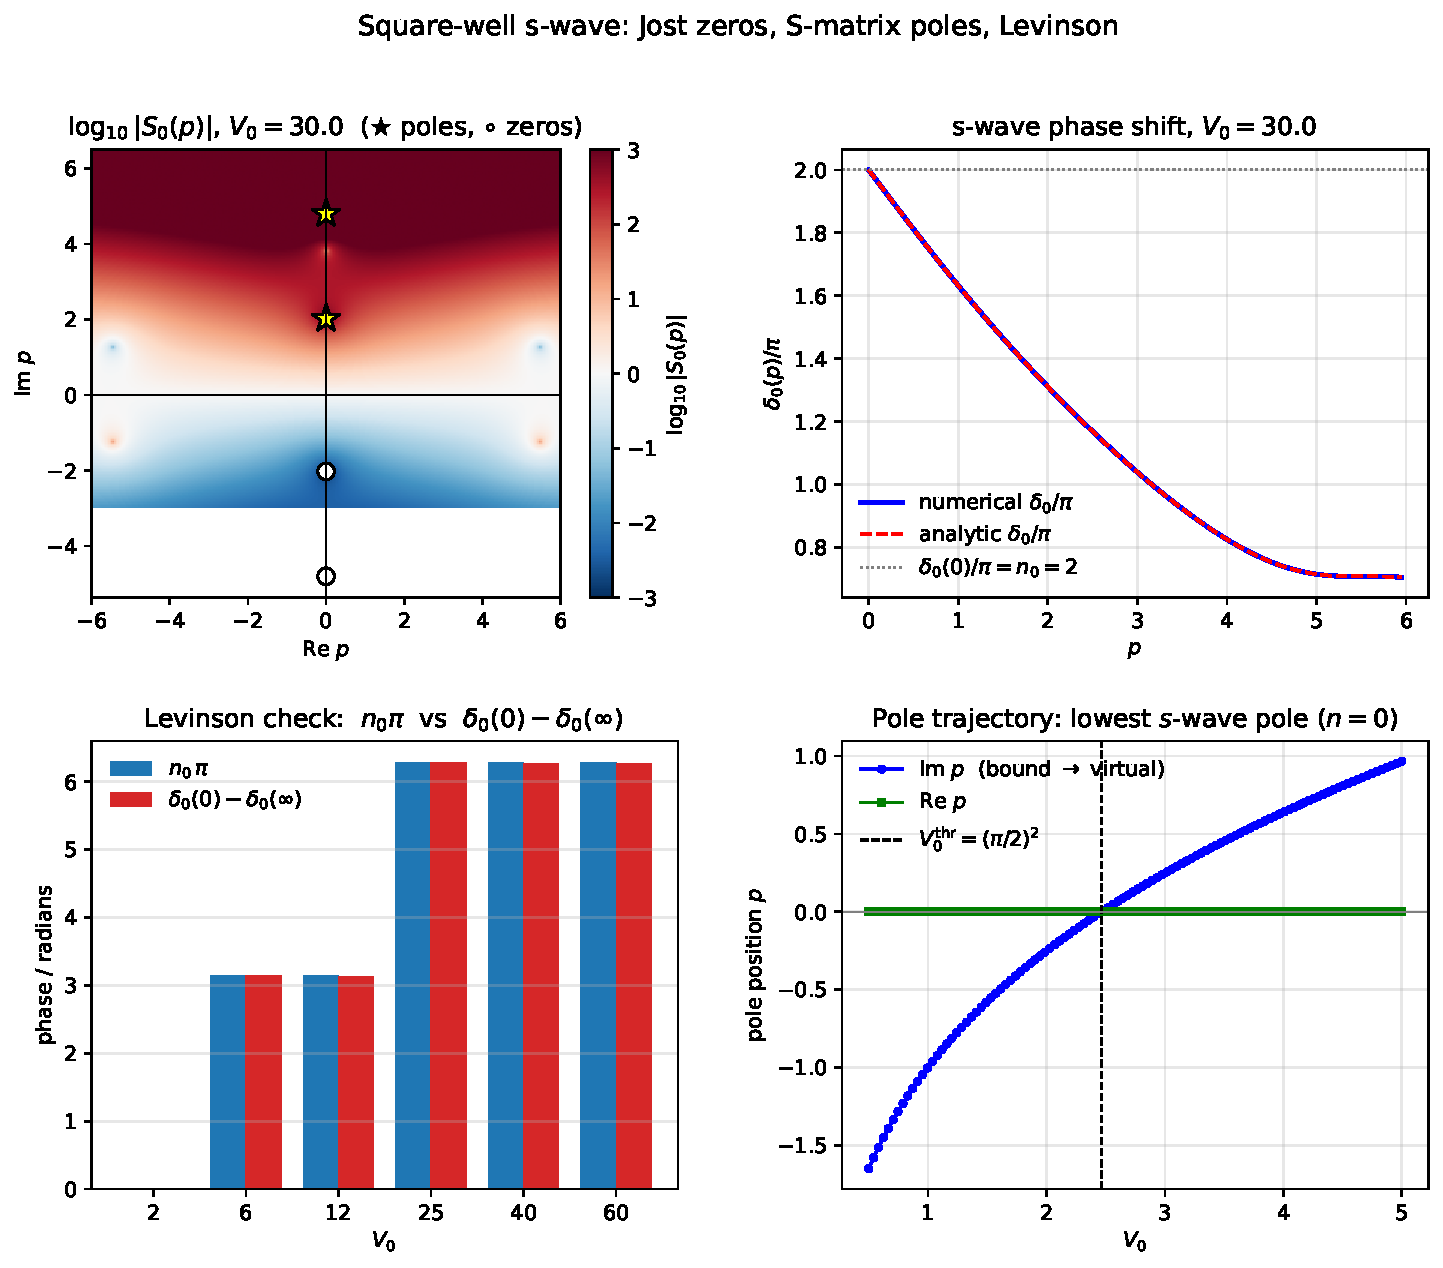
\includegraphics[width=0.95\linewidth]{ch11_jost_pole_levinson}
    \caption{方势阱 ($\hbar=2m=1,a=1$) s 波数值实验。
    \textbf{(左上)} $V_0=30$ 时复 $p$ 平面上 $\log_{10}|S_0(p)|$ 热图：
    黄色五角星标记上半平面 Jost 零点 $p=\rmi\kappa_{0,1}\approx\rmi\,2.022,\rmi\,4.800$ (S 矩阵极点)，
    白色圆点标记下半平面对应零点 ($S_0$ 的零点 $=\mathcal{F}_0(-p)$ 的零点)。
    \textbf{(右上)} 数值与解析相移对比：从 $\delta_0(0)/\pi=n_0=2$ 单调下降至 $0$，
    完全符合 Levinson 定理。
    \textbf{(左下)} 对一系列 $V_0$ 比较 $n_0\pi$ (束缚态计数) 与
    $\delta_0(0)-\delta_0(\infty)$ (相移积分)：两者数值上相等，相对误差 $<10^{-3}$。
    \textbf{(右下)} 当 $V_0$ 从 $5.0$ 降至 $0.5$ 时，最低 s 波 Jost 零点
    $p$ 沿虚轴向下穿过 $V_0^{\rm thr}=(\pi/2)^2\approx 2.467$ 时连续地由束缚态 $(\Im p>0)$
    转化为虚态 $(\Im p<0)$，$\Re p$ 始终为零 (s 波势阱中无共振分支)。}
    \label{fig:numexp-ch11}
\end{figure}

\subsection*{物理讨论}

\begin{enumerate}
\item \textbf{Jost 零点 $\leftrightarrow$ S 极点}：
由 $S_0(p)=\mathcal{F}_0(-p)/\mathcal{F}_0(p)$，$\mathcal{F}_0$ 的零点同时是 $S_0$ 的极点；
而 $\mathcal{F}_0(-p)$ 的零点是 $S_0$ 的零点。
解析延拓上 $\mathcal{F}_0(-p)=\overline{\mathcal{F}_0(\bar p)}$ (实势 Schwartz 反射)，
故上半平面的极点与下半平面的零点呈共轭分布
——这正是图 \ref{fig:numexp-ch11} 左上面板所展示的对称结构。

\item \textbf{束缚态、虚态、共振的统一刻画}：
    \begin{itemize}
    \item \emph{束缚态}: $p=\rmi\kappa$, $\kappa>0$, 即上半虚轴。能量 $E=-\kappa^2<0$ 物理上对应可归一束缚态。
    \item \emph{虚态}: $p=-\rmi\kappa$, $\kappa>0$, 即下半虚轴。同样对应实负能量但波函数发散，
          属第二叶。当势阱过浅以致最低束缚态消失时，对应的极点滑过 $p=0$ 进入下半轴成为虚态
          (右下面板)。两侧轨迹切线方向为 $\Im p\propto\pm\sqrt{|V_0-V_0^{\rm thr}|}$，对应阈
          能量行为 $E\propto V_0-V_0^{\rm thr}$。
    \item \emph{共振}: 第二叶上 $p_R=p_R'-\rmi p_R''$, $p_R'',p_R'>0$。s 波单纯方势阱不产生共振
          (无离心壁垒)，故图中未出现脱离虚轴的极点。共振在高分波或排斥壳中出现，将在
          \S\ref{ch:resonance} 集中讨论。
    \end{itemize}

\item \textbf{Levinson 定理 $\delta_0(0)-\delta_0(\infty)=n_0\pi$}：
左下面板把束缚态计数 $n_0$ (整数离散信息) 与连续相移 $\delta_0(p)$ 在物理域上的渐近差
(连续解析信息) 等同起来。
从全平面图像看，这是辐角原理 (argument principle)：
$\frac{1}{2\pi\rmi}\oint_C \frac{\mathcal{F}_0'(p)}{\mathcal{F}_0(p)}\,\rmd p=\#\text{零点}$，
取 $C$ 为上半平面无穷大半圆即得 Levinson；
该公式把分散在物理散射数据中的"积分相位"与上半平面"束缚态点谱"严格联系。
本数值实验取 $p_{\max}=2000$ 即足以让相移收敛到 $\delta_0(\infty)\bmod\pi=0$，
从而 $n_0\pi$ 与 $\delta_0(0)-\delta_0(\infty)$ 在 $\sim10^{-3}\pi$ 精度内吻合。

\item \textbf{阈值行为与零能反常}：
当 $V_0=V_0^{\rm thr}$ 时 $\mathcal{F}_0(0)=0$，即 S 矩阵在 $p=0$ 出现一阶极点，
散射长度 $a_s=-\lim_{p\to 0}\delta_0/p\to\infty$ (Wigner 散射阈值反常)。
右下面板的轨迹在 $V_0^{\rm thr}$ 处穿越原点，正是这一散射长度发散的直接图像。
冷原子物理中 Feshbach 共振调控正是利用了这种"束缚态—虚态"穿越机制。

\item \textbf{与全章解析结构的对应}：
方势阱不存在 Yukawa 型左割线 (势是紧支撑的)，故 $\mathcal{F}_0(p)$ 是整函数，
解析结构最为简洁——只有上下虚轴上的零点和左/右半平面的共振 (本例无)。
这恰好对应 \S\ref{ch:Smat1P} 提到的"截断势 $\Rightarrow$ Jost 函数解析至全平面"
的特殊情形，是检验本章一般理论的最干净的实验台。
\end{enumerate}

\chapter{共振 (Resonances)}\label{ch:resonance}

在前一章我们详细讨论了 Jost 函数 $f_\ell(p)$ 与分波 $S$ 矩阵元
$\mathsf{s}_\ell(p)=f_\ell(-p)/f_\ell(p)$ 在复 $p$ 平面上的解析性质，并指出
束缚态对应于 Jost 函数在正虚轴 $\Im p>0$ 上的零点（亦即 $\mathsf{s}_\ell$ 的极点）。
本章把这一框架推广到下半平面 $\Im p<0$：那里同样可能存在 $f_\ell$ 的零点，
它们对应于 $\mathsf{s}_\ell(p)$ 的极点，称为\textbf{共振极点 (resonance poles)}。
共振对应的能量 $E_R-\rmi\Gamma/2$ 位于复能量平面的下半叶（第二黎曼叶），
直接产生散射截面在 $E\approx E_R$ 处的尖锐峰，在时间演化中表现为
寿命 $\tau\sim\hbar/\Gamma$ 的亚稳态 (quasi-stationary state)。

参考资料：本章基于 Zhiguang 讲义第 12 讲，
并以 Taylor《Scattering Theory》第 13 章作为补充。

\section{共振的现象学}

实验上经常观测到散射截面 $\sigma(E)$ 作为入射能量 $E$ 的函数时
出现\emph{尖锐而隔离}的峰，例如：
\begin{itemize}
  \item 中子打铱核 (neutrons off iridium)：在 $\sim 1\,\mathrm{eV}$ 附近出现一系列
    宽度为 $\mathrm{meV}$ 量级的尖峰；
  \item $\pi^+$ 介子打质子 (pions off protons)：在总能量
    $\sim 1.2\,\mathrm{GeV}$ 处出现著名的 $\Delta(1232)$ 共振峰，
    宽度约 $100\,\mathrm{MeV}$。
\end{itemize}
这种现象意味着：在散射过程中，对某些特殊能量 $E_R$，
入射粒子与靶被短暂地俘获，形成一个接近束缚态的"亚稳态"
(quasi-stationary state)；该态会在有限寿命 $\tau$ 内衰变回散射末态。
当入射能量恰好接近 $E_R$ 时散射振幅被显著放大，从而使截面剧烈变化。

回忆束缚态对应 $\Im p>0$ 虚轴上 $f_\ell(p)$ 的零点 / $\mathsf{s}_\ell(p)$ 的极点。
后面我们将看到，共振对应 $\Im p<0$ 时 $f_\ell(p)$ 的零点 /
$\mathsf{s}_\ell(p)$ 的极点。

\begin{definition}[共振极点]\label{def:res-pole}
  设分波 $S$ 矩阵元 $\mathsf{s}_\ell(p)$ 可解析延拓至 $\Im p<0$ 的下半平面。
  若 $\mathsf{s}_\ell(p)$ 在 $\bar p=p_R-\rmi p_I$（$p_R>0,\;p_I>0$）处有一个
  孤立的极点，则称之为一个 \emph{共振极点}，对应的复能量
  \begin{equation}
    \bar E=\frac{\bar p^{\,2}}{2m}=E_R-\rmi\frac{\Gamma}{2},\qquad
    E_R=\frac{p_R^2-p_I^2}{2m},\quad \Gamma=\frac{2 p_R p_I}{m},
  \end{equation}
  其中 $E_R>0$ 称为\emph{共振能量}，$\Gamma>0$ 称为\emph{共振宽度}，
  对应的寿命为 $\tau=1/\Gamma$（自然单位 $\hbar=1$）。
\end{definition}

\section{$\mathsf{s}_\ell$ 矩阵的下半平面极点与共振相移}

设 $f_\ell(p)$ 可被解析延拓至 $\Im p<0$ 的下半 $p$-平面，
则在接近实轴处 $\bar p=p_R-\rmi p_I$（$p_R>0,p_I>0$）一般会有
一个零点。由 $\mathsf{s}_\ell(p)=f_\ell(-p)/f_\ell(p)$ 知 $\bar p$
对应 $\mathsf{s}_\ell(p)$ 的极点。我们考察 $f_\ell$ 在该点附近的行为
（假设是单零点且离实轴足够近）：
\begin{equation}
  f_\ell(p)\simeq\left(\frac{\rmd f_\ell}{\rmd p}\right)_{\bar p}(p-\bar p)
  ,\qquad \bar p=p_R-\rmi p_I.
\end{equation}

\subsection{零点处的"波函数"}

回顾上一章 Jost 解的归一化关系，在零点 $\bar p$ 处约化波函数
满足
\begin{equation}
  \phi^+_{\ell,\bar p}(r)\propto f_\ell(-\bar p)\chi^+_{\ell,\bar p}(r),
  \qquad \chi^+_{\ell,\bar p}(r)\sim\rme^{\rmi\bar p r}=\rme^{\rmi p_R r}\rme^{p_I r}
\end{equation}
即在 $r\to\infty$ 时\emph{指数发散}（因为 $p_I>0$）。
故 $\phi^+_{\ell,\bar p}$ 不是平方可积的，并不构成希尔伯特空间中的
本征矢；但它仍可形式上视为 $\Hmat$ 的"广义本征矢"，本征值为
$\bar E=E_R-\rmi\Gamma/2$。这种发散波函数在文献中称为
\emph{Gamow 态}或\emph{Siegert 态}，描写一个"只有外行波"的衰变态。

\subsection{共振相移}

考虑 $p$ 沿正实轴扫过 $p_R$ 时的相移行为。由
$\mathsf{s}_\ell(p)=\rme^{2\rmi\delta_\ell(p)}$，且
$f_\ell(-p)$ 在 $\bar p$ 邻域基本是常数（无零点附近的奇异行为），
\begin{align}
  \delta_\ell(p)
  &\approx -\arg\!\left(\frac{\rmd f_\ell}{\rmd p}\right)_{\bar p}-\arg(p-\bar p)\nonumber\\
  &\equiv \delta_{\mathrm{bg}}+\delta_{\mathrm{res}}(p),
  \qquad
  \delta_{\mathrm{res}}(p)\equiv -\arg(p-\bar p) \pmod\pi .
\end{align}
其中 $\delta_{\mathrm{bg}}$ 视作\emph{背景相移}（在共振附近近似为常数），
$\delta_{\mathrm{res}}$ 是\emph{共振部分}。
观察 $p\in\mathbb R$ 从 $-\infty$ 到 $+\infty$：
矢量 $p-\bar p=(p-p_R)+\rmi p_I$ 始终位于上半 $p$-平面，
其辐角从接近 $\pi$ 减到接近 $0$，所以 $\delta_{\mathrm{res}}(p)$
从 $0$ 增至 $\pi$。当 $p$ 接近 $p_R$ 时变化最快——这就是
共振处相移\emph{快速上升 $\pi$} 的几何来源。

\begin{remark}
  四种典型情形（Taylor 图 13.3）：把背景相移取作
  $\delta_{\mathrm{bg}}=0,\pi/4,\pi/2,3\pi/4$，则
  $\sin^2\delta_\ell(p)$（即分波截面 $\sigma_\ell\propto\sin^2\delta_\ell$
  除去 $4\pi(2\ell+1)/p^2$ 因子）展示出标准的
  \emph{对称峰}（$\delta_{\mathrm{bg}}=\pi/2$，最显著的"共振峰"），
  \emph{对称谷}（$\delta_{\mathrm{bg}}=0$，从 0 升到 $\pi$，$\sin^2$ 在 $\pi/2$ 处达极大），
  和\emph{峰-谷不对称}的形状（Fano-like profile）。
  在 $\delta_{\mathrm{bg}}=0$ 的"理想"情形下，
  \begin{equation}
    \sigma_\ell=\frac{4\pi(2\ell+1)}{p^2}\sin^2\delta_\ell(p),
  \end{equation}
  共振附近 $\sin^2\delta_\ell$ 经过 $1$ 的极大，并具备
  Breit-Wigner 形状（见 \S\ref{sec:BW}）。
\end{remark}

\section{复能量平面与黎曼叶结构}\label{sec:Eplane}

由变换 $E=p^2/2m$，$p$-平面的上半与下半映射到 $E$-平面的两叶
（黎曼面 Riemann surface），切割沿 $E\geq 0$ 实轴。具体地：
\begin{itemize}
  \item $f_\ell(p),\;\Im p>0$ $\;\longrightarrow\;$ $f_\ell^I(E)$，零点对应 $\mathsf{s}_\ell^I(E)$ 极点；
  \item $f_\ell(-p),\;\Im p>0$ $\;\longrightarrow\;$ $f_\ell^{II}(E)$，零点对应 $\mathsf{s}_\ell^{II}(E)$ 极点。
\end{itemize}
每叶 $E$-平面都有一个沿正实轴的割线 $E\geq 0$。
\begin{itemize}
  \item 第一叶（\emph{物理叶, physical sheet}, $\Im p>0$）割线上沿对应
    $p>0$ 正实轴上沿；下沿对应 $p<0$ 实轴下沿。
    第二叶（\emph{非物理叶, second sheet}, $\Im p<0$）割线上沿则对应
    $p<0$ 实轴上沿、下沿对应 $p>0$ 实轴下沿。
  \item \textbf{束缚态}：$p$-平面正虚轴 $\;\to\;$ $E$-平面第一叶负实轴；
  \item \textbf{虚态 (virtual state)}：$p$-平面下半负虚轴 $\;\to\;$
    $E$-平面第二叶负实轴；能量为负但无虚部，与束缚态对称但位于第二叶；
  \item \textbf{共振态 (resonance)}：$p$-平面下半 $\Im p<0$、$\Re p>0$ 区域
    $\;\to\;$ $E$-平面第二叶复平面（能量含负虚部 $-\Gamma/2$）。
    共振极点成对出现：$\bar p=\pm p_R-\rmi p_I$ 对应于
    $\bar E$ 与 $\bar E^*$，因为 $f_\ell(p)$ 在物理意义下满足
    $f_\ell(p^*)=f_\ell(-p)^*$（实势）。
\end{itemize}

\begin{remark}
  $\mathsf{s}_\ell(E)$ 在 $E$-平面第一叶除了负实轴上的束缚态极点外，
  没有其他奇点（这是因果性 + 解析性的体现）；
  但其零点（位于第一叶）与第二叶上的极点一一对应：由
  \begin{equation}
    \mathsf{s}_\ell^{II}(E)=\frac{f_\ell(p)}{f_\ell(-p)}=\frac{1}{\mathsf{s}_\ell^{I}(E)},
  \end{equation}
  第一叶 $\mathsf{s}_\ell^I(E)$ 的零点直接给出第二叶 $\mathsf{s}_\ell^{II}(E)$
  的极点。在相对论散射理论中也有完全类似的两叶 / 多叶结构。
\end{remark}

\subsection{Breit--Wigner 公式}\label{sec:BW}

当共振极点 $\bar E=E_R-\rmi\Gamma/2$ 距离物理实轴很近（即
$\Gamma\ll E_R$，窄共振条件）时，可以把 $f_\ell$ 在 $\bar E$ 附近 Taylor
展开到首项：
\begin{equation}
  f_\ell(E)\approx\left(\frac{\rmd f}{\rmd E}\right)_{\bar E}(E-\bar E),
  \qquad
  \delta_\ell(E)\approx \delta_{\mathrm{bg}}+\delta_{\mathrm{res}}(E),
\end{equation}
经过简单几何（$\delta_{\mathrm{res}}=-\arg(E-\bar E)$）得
\begin{equation}\label{eq:BW-sin}
  \sin\delta_{\mathrm{res}}(E)
  =\frac{\Gamma/2}{[(E-E_R)^2+(\Gamma/2)^2]^{1/2}}.
\end{equation}
若背景相移 $\delta_{\mathrm{bg}}\approx 0$，则分波截面为
\begin{equation}\label{eq:BW-sigma}
  \boxed{\;\sigma_\ell(E)\;\sim\;\sin^2\delta_\ell(E)
  \;=\;\frac{(\Gamma/2)^2}{(E-E_R)^2+(\Gamma/2)^2}\;}
\end{equation}
这就是著名的 \textbf{Breit--Wigner 公式}：散射截面是关于 $E_R$ 对称的洛伦兹型
峰，半高全宽即为 $\Gamma$。等价地，对应的分波振幅可写成
\begin{equation}\label{eq:BW-fl}
  f_\ell(E)\;\approx\;-\frac{\Gamma/2}{E-E_R+\rmi\Gamma/2}
  \quad(\text{对零背景相移})，
\end{equation}
$\mathsf{s}_\ell(E)\approx \dfrac{E-E_R-\rmi\Gamma/2}{E-E_R+\rmi\Gamma/2}$，
显式地展示极点 $E_R-\rmi\Gamma/2$ 在第二叶下半平面。

\begin{remark}
  若背景相移不为零，则 \eqref{eq:BW-sigma} 应替换为
  $\sigma_\ell\sim\sin^2(\delta_{\mathrm{bg}}+\delta_{\mathrm{res}})$，
  导致截面出现典型的"峰-谷"不对称 (Fano profile)；这正是
  \S\ref{sec:Eplane} 节图 13.3 中四种情形的来源。
\end{remark}

\begin{example}[$\Delta$ 共振拟合]
  $\pi^+ p\to\Delta^{++}\to\pi^+ p$ 在 $\sqrt{s}\approx 1232\,\mathrm{MeV}$、
  $\Gamma\approx 117\,\mathrm{MeV}$、$\ell=1$ ($P$ 波，$J^P=3/2^+$)
  上的截面在峰附近可被 \eqref{eq:BW-sigma} 很好地拟合，扣除背景后是个
  典型的洛伦兹峰。
\end{example}

\section{束缚态、虚态与共振态：极点的迁移}

随着耦合强度（势的强度）的变化，束缚态、虚态和共振之间会
互相转换。考虑势 $V$ 引入耦合常数 $\lambda$：
\begin{equation}
  H=H^0+\lambda V .
\end{equation}
Jost 函数 $f_\ell(\lambda,p)$ 关于 $p$ 在 $\Im p\geq 0$ 解析（除原点），
作为 $(\lambda,p)$ 的函数也是解析的。考察 $f_\ell$ 的零点
随 $\lambda$ 的迁移：设在某 $\lambda_0$ 处 $f_\ell$ 在 $p=0$ 有一个零点
（即恰好出现"零能共振 / 零能束缚态"的临界耦合）。

围绕 $(\lambda_0,0)$ 做幂级数展开
\begin{equation}
  f_\ell(\lambda,p)=\sum_{m,n}\alpha_{mn}p^m(\lambda-\lambda_0)^n .
\end{equation}

\subsection{$\ell=0$（$s$ 波）}

由对称性与已知的 $f_0(p)$ 的奇偶结构，展开首项为
\begin{equation}
  f_0(\lambda,p)=\rmi\xi p+\eta(\lambda-\lambda_0)+\cdots ,
\end{equation}
零点在
\begin{equation}
  \bar p\approx -\rmi\frac{\eta}{\xi}(\lambda-\lambda_0),
\end{equation}
即沿\emph{虚轴线性移动}：当 $\lambda$ 朝吸引方向变（$\eta(\lambda-\lambda_0)<0$
使 $-\rmi\eta(\lambda-\lambda_0)/\xi$ 正虚部为正），零点跑到 $\Im p>0$，
变成束缚态；反之 $\lambda$ 朝排斥方向变，零点跑到 $\Im p<0$ 的负虚轴上，
对应能量为负、无虚部的\textbf{虚态 (virtual state)}。
\begin{itemize}
  \item 注意 $\ell=0$ 时是\emph{一阶零点}，故跨越 $p=0$ 时只产生一个零点
    沿虚轴上下移动，没有变成共振对。
\end{itemize}

\subsection{$\ell>0$（高分波）}

由角动量势垒导致的 $p^{2\ell}$ 行为，$f_\ell$ 在 $p=0$ 附近最低阶为 $p^2$
（更准确地，$f_\ell$ 在 $p=0$ 附近的展开系数包含 $p^{2\ell+1}$ 之外的
偶次项），可写
\begin{equation}
  f_\ell(\lambda,p)=\xi p^2+\eta(\lambda-\lambda_0)+\cdots
\end{equation}
零点
\begin{equation}\label{eq:res-pair}
  \bar p\approx \pm \rmi\sqrt{\eta(\lambda-\lambda_0)/\xi}
  \;=\;\pm \rmi\!\left(\frac{\eta}{\xi}\right)^{\!1/2}(\lambda-\lambda_0)^{1/2}.
\end{equation}
注意这是\emph{二阶零点}，故 $\lambda$ 跨过 $\lambda_0$ 时
两个零点从虚轴上对称地脱离，进入下半平面变成
$\bar p$ 与 $-\bar p^*$ 一对共振极点（对实势 $V$，零点对称分布）。
更细致地（并保留 $p^2$ 与 $p^{2\ell+1}$ 的相对贡献）有
\begin{equation}
  f_\ell(p)=1+[\alpha_\ell+\beta_\ell p^2+O(p^4)]+\rmi[\gamma_\ell p^{2\ell+1}+O(p^{2\ell+3})],
  \qquad 1+\alpha_\ell\sim\eta(\lambda-\lambda_0),\;\beta_\ell\sim\xi.
\end{equation}
由此可看出 $|\Im\bar p|\sim(\lambda-\lambda_0)^\ell$（高分波两共振极点
分开时\emph{离实轴更近}），即\emph{$\ell$ 越大，新生成的共振越尖锐}。
这反映了角动量势垒抑制衰变、提高寿命的物理图像。

\begin{itemize}
  \item $p=0$ 附近背景相移较小：$\lambda<\lambda_0$ 朝吸引方向偏，
    则有束缚态，$\rmd f/\rmd E$ 实部为主，相移随 $E$ 缓慢变化。
  \item $\lambda>\lambda_0$ 后，$\rmd f/\rmd E$ 虚部为主、实部小，
    $\arg(\rmd f/\rmd E)$ 较小，故共振 Breit--Wigner 公式的"零背景"近似成立，
    共振峰对称且尖锐。
\end{itemize}

\subsection{方势阱中的相移演化（$\ell=3$ 例）}

考虑球方势阱 $V(r)=-V_0\theta(a-r)$，固定 $a$ 改变深度 $V_0$，
观察 $\ell=3$ 的相移 $\delta_3(p)$ 与分波截面 $\sigma_3(p)$
（图见 Taylor 13.4）：
\begin{itemize}
  \item $V_0$ 小（$2ma^2 V_0=5.2$）：吸引尚不足以形成束缚态，但已经存在
    一个\emph{共振}：$\delta_3$ 在某个 $p$ 附近上升约 $\pi$，
    $\sigma_3$ 出现尖锐峰；
  \item 加深 $V_0$（$2ma^2 V_0=5.5,\;5.7$）：共振变窄并下移
    （$E_R\to 0$），最后在 $V_0$ 临界值时变成 $E=0$ 的零能共振；
  \item 再加深（$2ma^2 V_0=5.8$）：共振"穿过" $E=0$ 进入物理叶
    成为一个\emph{束缚态}，相移突然变成 $\delta_3(0)=\pi$（Levinson 定理：
    束缚态数 $n_3$ 增加 $1$，对应 $\delta_3(0)$ 跃升 $\pi$），
    高能处 $\delta_3$ 平缓不再出现共振峰。
\end{itemize}
这个例子完整展示了"共振 $\to$ 零能束缚态 $\to$ 真束缚态"的极点迁移过程。

\section{有共振时的散射过程}\label{sec:scatt-with-res}

我们现在重新考虑\emph{波包}打入靶后的散射过程，看共振态如何
影响散射波的时间和空间分布。回忆第 \ref{ch:resonance} 章中
散射波的渐近形式
\begin{equation}
  \psi(\mathbf x,t)=\psi_{\mathrm{in}}(\mathbf x,t)+\psi_{\mathrm{sc}}(\mathbf x,t),
\end{equation}
\begin{equation}\label{eq:psi-sc-asymp}
  \psi_{\mathrm{sc}}(\mathbf x,t)\xrightarrow{r\to\infty}
  (2\pi)^{-3/2}\frac{1}{r}\int\rmd^3 p\,\phi(\mathbf p)\,
  f(p\hat{\mathbf x}\leftarrow\mathbf p)\,\rme^{\rmi(p r-E t)}.
\end{equation}
以前在"光滑振幅"的近似下我们把 $f$ 看成在 $\phi(\mathbf p)$
的支集上几乎不变，得到
\begin{equation}
  \psi_{\mathrm{sc}}\xrightarrow{r\to\infty}\frac{1}{r}f(p_0\hat{\mathbf x}\leftarrow\mathbf p_0)\,
  \psi_{\mathrm{in}}(r\hat{\mathbf 3},t).
\end{equation}
但若入射波包能量分布跨越共振 $E_R$、宽度 $\Gamma$，就要分两种
情形讨论：
\begin{description}
  \item[(1) $\Delta E\ll\Gamma$（高分辨率）：] 入射波包能量分布远比共振宽度
    窄，实验分辨率\emph{足以}解出共振峰（看到尖峰）。但 $f$ 在
    $\Delta E$ 范围内仍可视为缓慢变化。
  \item[(2) $\Delta E\gg\Gamma$（低分辨率）：] 入射波包能量分布远宽于共振，
    实验上看不出共振峰；散射波被共振"延迟"，表现为亚稳态衰变波。
\end{description}

\subsection{情形 (1)：$\Delta E\ll\Gamma$ —— Wigner 时间延迟}

设只有第 $\ell$ 分波有共振，能量 $E_R$，宽度 $\Gamma$，
其他分波相移可以忽略。则
\begin{equation}
  f(p_0\hat{\mathbf x}\leftarrow\mathbf p_0)
  =(2\ell+1)f_\ell(p_0)P_\ell(\hat{\mathbf p}'\cdot\hat{\mathbf p})
  =(2\ell+1)\frac{\rme^{\rmi\delta_\ell}\sin\delta_\ell}{p}P_\ell(\hat{\mathbf p}'\cdot\hat{\mathbf p}).
\end{equation}
$\phi(\mathbf p)$ 的能量峰仍然很尖锐（$\Delta E\ll\Gamma\ll E_R$），
故可以把 $\delta_\ell(p)\approx\delta_\ell(p_0)+\delta'_\ell(p_0)(p-p_0)$
线性展开。注意出射散射波携带相位 $2\delta_\ell$（即 $\mathsf{s}_\ell=e^{2\rmi\delta_\ell}$），
代入 \eqref{eq:psi-sc-asymp}：
\begin{align}
  \rme^{2\rmi\delta_\ell}&\approx \exp\{2\rmi[\delta_\ell(p_0)+\delta'_\ell(p_0)(p-p_0)]\}
  =\mathrm{const}\times \exp[2\rmi\delta'_\ell(p_0) p],\nonumber\\
  \mathrm{const}&=\rme^{2\rmi[\delta_\ell(p_0)-\delta'_\ell(p_0)p_0]}.
\end{align}
故
\begin{align}
  \psi_{\mathrm{sc}}(\mathbf x,t)
  &\xrightarrow{r\to\infty}\mathrm{const}\,\frac{P_\ell(\cos\theta)}{r}\!\int\!\rmd^3 p\,\phi(\mathbf p)\,(2\ell+1)\,
    \rme^{\rmi[p(r+2\delta'_\ell)-Et]}\nonumber\\
  &\approx \mathrm{const}\,\frac{P_\ell(\cos\theta)}{r}\,
    \psi_{\mathrm{in}}\!\big[(r+2\delta'_\ell)\hat{\mathbf 3},\,t\big]\nonumber\\
  &= \frac{f_\ell(p_0\hat{\mathbf x}\leftarrow\mathbf p_0)}{r}\,
    \psi_{\mathrm{in}}\!\big[(r+2\delta'_\ell)\hat{\mathbf 3},\,t\big].
\end{align}
散射波的"位置"恰为入射波包在 $r+2\delta'_\ell$ 处的样子，即比无相互作用情况
\emph{滞后了一段距离}
\begin{equation}\label{eq:wigner-xi}
  \xi=2\delta'_\ell(p)\equiv\frac{\rmd(2\delta_\ell)}{\rmd p}=2v_0\,\frac{\rmd\delta_\ell}{\rmd E},
\end{equation}
对应的\textbf{Wigner 时间延迟}为
\begin{equation}\label{eq:wigner-tau}
  \tau=\frac{\xi}{v_0}=\frac{2}{v_0}\frac{\rmd\delta_\ell}{\rmd p}\bigg|_{p_0}
  =2\frac{\rmd\delta_\ell}{\rmd E}\bigg|_{p_0}.
\end{equation}
即可视为入射粒子在中间形成了一个亚稳态被"俘"住，然后在时间 $\tau$ 后
衰变成末态。

\begin{remark}[因果性约束]
  若 $\delta_\ell'(p)<0$，散射波\emph{超前}于无相互作用情形。
  但这种"超前"不可能超过靶子大小 $a$（否则散射波在入射波到靶之前就已存在，
  破坏因果性），故有上限
  \begin{equation}
    \frac{\rmd\delta_\ell}{\rmd p}\geq -a,\qquad \tau\geq -\frac{a}{v_0}.
  \end{equation}
  即\emph{相移的斜率不能比 $-a$ 更陡}。
\end{remark}

\begin{remark}[对截面的影响]
  在该情形下散射截面仍由 $|f_\ell|^2$ 给出，并显示 Breit--Wigner 峰：
  \begin{equation}
    \frac{\rmd\sigma}{\rmd\Omega}=|f|^2,
  \end{equation}
  共振峰使得 $\rmd\sigma/\rmd\Omega$ 出现\emph{峰}（$\delta_{\mathrm{bg}}\approx 0$）
  或\emph{峰-谷}结构（背景非零）。
\end{remark}

\begin{remark}[延迟距离与波包大小]
  上述图像有些"夸张"，实际上在 $\Delta E\ll\Gamma$ 条件下，
  入射波包大小为 $\sim 1/\Delta p$，而延迟距离
  \begin{equation}
    \xi=v_0\frac{\rmd\delta_\ell}{\rmd E}\sim \frac{v_0}{\Gamma}
    \;\ll\;\frac{1}{\Delta E/v_0}=\frac{1}{\Delta p}\sim\text{packet size}.
  \end{equation}
  即延迟距离 $\xi$ \emph{远小于波包大小}，入射波包和散射波包仍有大量重叠。
  因此分辨"延迟"在波包图像中并不直接对应一个明显的"间隙"，
  而是体现在干涉中。
\end{remark}

\subsection{情形 (2)：$\Delta E\gg\Gamma$ —— 共振态的衰变}

假设背景相移很小，散射振幅主要由共振贡献——使用 \eqref{eq:BW-fl}：
\begin{equation}
  \mathsf{s}_\ell=\frac{E-E_R-\rmi\Gamma/2}{E-E_R+\rmi\Gamma/2},\qquad
  f_\ell=-\frac{1}{p}\,\frac{\Gamma/2}{E-E_R+\rmi\Gamma/2}.
\end{equation}
代入 \eqref{eq:psi-sc-asymp}：
\begin{equation}
  \psi_{\mathrm{sc}}(\mathbf x,t)\xrightarrow{r\to\infty}
  \mathrm{const}\!\int\!\rmd^3 p\,
  \frac{(2\ell+1)\phi(\mathbf p)P_\ell(\hat{\mathbf x}\cdot\hat{\mathbf p})}
  {2p(E-E_R+\rmi\Gamma/2)}\,\Gamma\,\rme^{\rmi(p r-E t)}.
\end{equation}
$\phi(\mathbf p)$ 在 $\mathbf p_0$ 附近峰值集中（设 $\phi(\mathbf p)=\frac{1}{\sqrt{mp}}\sum_\ell \phi_\ell(p)Y^0_\ell(\hat{\mathbf p})$），
取角度积分挑出 $\ell$ 分波后
\begin{equation}
  \psi_{\mathrm{sc}}\;\approx\;\mathrm{const}\,
  \frac{Y^0_\ell(\cos\theta)}{r}\int_0^\infty\!\rmd p\,p^{1/2}\,
  \frac{\phi_\ell(E)\,\Gamma\,\rme^{\rmi(p r-E t)}}{E-E_R+\rmi\Gamma/2}.
\end{equation}
利用 $p\approx p_R+(E-E_R)/v_R$（$v_R=p_R/m$ 为共振速度）作变换
$p\rmd p=m\rmd E$：
\begin{align}
  \psi_{\mathrm{sc}}(\mathbf x,t)
  &= \mathrm{const}\,\frac{Y_\ell^0(\cos\theta)\phi_\ell(E_R)\,\rme^{\rmi[p_R r-E_R t]}}{p_R^{1/2}\,r}\!
     \int_0^\infty\!\rmd E\,\frac{\Gamma\,\rme^{-\rmi(E-E_R)(t-r/v_R)}}{E-E_R+\rmi\Gamma/2} .
\end{align}
将下限近似延伸到 $-\infty$（因 $\phi_\ell(E)$ 在 $\Delta E\gg\Gamma$
范围内变化缓慢，对积分主要贡献来自共振极点附近），由柯西定理：
对 $t>r/v_R$ 在下半 $E$-平面闭合，包围共振极点 $E_R-\rmi\Gamma/2$；
对 $t<r/v_R$ 在上半闭合无极点，故得
\begin{equation}
  \int_{-\infty}^{\infty}\!\rmd E\,\frac{\Gamma\,\rme^{-\rmi(E-E_R)(t-r/v_R)}}{E-E_R+\rmi\Gamma/2}
  =-2\pi\rmi\,\Gamma\,\rme^{-\Gamma(t-r/v_R)/2}\theta(t-r/v_R).
\end{equation}
因此
\begin{equation}\label{eq:psi-sc-decay}
  \psi_{\mathrm{sc}}(\mathbf x,t)\approx
  \mathrm{const}\,\frac{Y_\ell^0(\cos\theta)\phi_\ell(E_R)\,\rme^{\rmi[p_R r-E_R t]}}{p_R^{1/2}\,r}\cdot
  (2\pi\rmi)\,\rme^{-\frac{\Gamma}{2}(t-r/v_R)}\theta(t-r/v_R).
\end{equation}
两边取模平方：
\begin{equation}\label{eq:psi-sc-decay-sq}
  \boxed{\;|\psi_{\mathrm{sc}}(\mathbf x,t)|^2
  =2\pi m\,\Gamma\,|Y_\ell^0(\cos\theta)\phi_\ell(E_R)|^2\,
  \frac{\rme^{-\Gamma(t-r/v_R)}}{p_R r^2}\,\theta(t-r/v_R) .\;}
\end{equation}

\paragraph{物理解读：}

\begin{itemize}
  \item 在 $r$ 处放一个探测器，则在 $t<r/v_R$ 时\emph{看不到}散射态：
    阶跃 $\theta(t-r/v_R)$ 体现了\emph{因果性}（信号需要时间
    $r/v_R$ 才能从靶传到探测器）。
  \item 在 $t>r/v_R$ 时观测到的角分布为 $|Y_\ell^0(\hat{\mathbf x})|^2$，
    强度按\emph{指数衰减} $\rme^{-\Gamma t}$，
    寿命为 $\tau=1/\Gamma$。
  \item 整个过程相当于：在 $t=0$ 时刻形成了一个\emph{角动量为 $\ell$
    的亚稳态 (Gamow 态)}，能量 $E_R$，衰变宽度 $\Gamma$，寿命 $1/\Gamma$；
    它以速度 $v_R$ 向外发出指数衰减的球面波。
  \item 此时 $\Gamma\ll\Delta E$，散射截面公式由对入射能量分布做平均得到
    \begin{equation}
      \frac{\rmd\sigma}{\rmd\Omega}=\frac{2\pi^2(2\ell+1)}{p_R^2}\,\Gamma\,w(E_R)\,|Y_\ell^0(\hat{\mathbf p})|^2,
      \qquad w(E)=\frac{p}{m}\!\int\!\rmd\Omega\,|\phi(\mathbf p)|^2,
    \end{equation}
    即截面正比于 $\Gamma$，反映出共振的\emph{产生率}与衰变宽度
    成正比（黄金法则）。
\end{itemize}

\begin{remark}[Gamow / Siegert 态]\label{rem:gamow}
  上面 \eqref{eq:psi-sc-decay} 中 $\rme^{-\Gamma t/2}\rme^{-\rmi E_R t}=
  \rme^{-\rmi\bar E t}$，即整个亚稳态表现为
  能量 $\bar E=E_R-\rmi\Gamma/2$、波函数 $\sim \rme^{\rmi p_R r}\rme^{p_I r}$
  的"广义本征态"——这正是 $f_\ell$ 在 $\bar p$ 零点处对应的发散波函数
  Gamow 态。它\emph{不属于} $\Hilb=L^2(\R^3)$，但在描写"开放系统"中
  亚稳态的衰变时是物理可解释的。
\end{remark}

\begin{remark}[指数衰变律的偏离]
  严格说来，把积分下限从 $0$ 延到 $-\infty$ 是个近似。在
  极短时刻（$t\ll 1/E_R$）和极长时刻（$t\gg \tau\ln(E_R/\Gamma)$）
  都会出现对纯指数衰变的偏离：
  \begin{itemize}
    \item \emph{短时}：
      $1-|\langle\psi(0)|\psi(t)\rangle|^2 \sim t^2$ 而非 $\Gamma t$，
      这是 Khalfin 定理的一部分；它与"量子 Zeno 效应"有关。
    \item \emph{长时}：来自割线（$E\geq 0$ 物理域）的贡献，
      给出幂次衰减 $\sim t^{-3}$ 等代数尾，依赖于阈值附近 $f_\ell$ 的解析结构。
  \end{itemize}
  在实际共振寿命范围内（$1/E_R\ll t\ll \tau\ln(E_R/\Gamma)$），
  指数律 $\rme^{-\Gamma t}$ 是极好的近似。
\end{remark}

\section{小结}

本章主要内容总结如下：
\begin{enumerate}
  \item \textbf{共振极点的位置}：共振对应 $f_\ell(p)$ 在下半 $p$-平面
    （$\Im p<0,\;\Re p>0$）的零点，亦即 $\mathsf{s}_\ell(p)$ 的极点；
    复能量为 $\bar E=E_R-\rmi\Gamma/2$，位于 $E$-平面的\emph{第二叶}下半平面。
  \item \textbf{能量平面黎曼面}：$E$-平面是两叶黎曼面，沿 $E\geq 0$ 切割。
    第一叶为物理叶（$\Im p>0$），第二叶为非物理叶（$\Im p<0$）。
    束缚态：$p$-平面正虚轴 / $E$-平面第一叶负实轴上的极点。
    虚态：$E$-平面第二叶负实轴上的极点（与束缚态实轴对称）。
    共振态：$E$-平面第二叶复平面上的极点。
  \item \textbf{$\mathsf{s}$ 矩阵的对称性}：$\mathsf{s}_\ell^I(E)$ 第一叶上的零点
    一一对应 $\mathsf{s}_\ell^{II}(E)$ 第二叶的极点
    （$\mathsf{s}^{II}=1/\mathsf{s}^I$）。
  \item \textbf{Breit--Wigner 公式}：在窄共振、零背景相移下
    \begin{equation*}
      f_\ell(E)\approx -\frac{\Gamma/2}{E-E_R+\rmi\Gamma/2},\qquad
      \sigma_\ell\sim\frac{(\Gamma/2)^2}{(E-E_R)^2+(\Gamma/2)^2}.
    \end{equation*}
    相移 $\delta_\ell$ 在 $E_R$ 附近上升 $\pi$。
  \item \textbf{束缚态与共振态相互转换}：连续改变耦合 $\lambda$，
    \begin{itemize}
      \item $\ell=0$：单个束缚态极点过 $p=0$ 进入下半平面变为虚态；
      \item $\ell>0$：束缚态极点经零能后\emph{分裂为一对共振极点}
        （\eqref{eq:res-pair}）。$\ell$ 越大，共振离实轴越近、越尖锐。
    \end{itemize}
  \item \textbf{中间共振散射}：
    \begin{enumerate}
      \item 当 $\Delta E\ll \Gamma$（高分辨率），散射波相对无相互作用情况
        \emph{滞后}距离 $\xi=\delta'_\ell(p)$（Wigner 时间延迟
        $\tau=\rmd\delta_\ell/\rmd E$）；
      \item 当 $\Delta E\gg \Gamma$（低分辨率），可视为 $t=0$ 时形成
        角动量 $\ell$ 的亚稳态，衰变宽度 $\Gamma$、寿命 $1/\Gamma$，
        散射波呈球面指数衰减 $\rme^{-\Gamma t}$、阶跃 $\theta(t-r/v_R)$。
    \end{enumerate}
\end{enumerate}

至此，对共振态在散射理论中的描述——从 $S$ 矩阵的复极点结构、
能量平面的黎曼面拓扑，到截面的 Breit--Wigner 形式与时域内的指数衰变——
形成了一个统一而自洽的图像。它把
\emph{束缚态、虚态、共振态}全部纳入同一个解析延拓的框架，
是非相对论散射理论最深刻的成就之一，并直接推广至相对论共振、
原子核反应、乃至粒子物理中的所有不稳定态。

%==============================================================================
\section{本章定理证明补全}\label{sec:res-proofs}
%==============================================================================

本节集中给出本章四个核心论断的完整证明：
(i) 由"第二叶单极点 + 单位性"推出严格的 Breit--Wigner 形式；
(ii) 用稳态相位法在高斯波包上严格导出 Wigner 时间延迟
$\tau=2\,\rmd\delta/\rmd E$；
(iii) Khalfin 关于长时偏离指数衰变的定理；
(iv) Friedrichs 模型的精确解，给出可控的"嵌入本征值
$\to$ 复极点 $\to$ 指数衰变"机制。

%------------------------------------------------------------------------------
\subsection{Breit--Wigner 公式的严格证明}\label{subsec:res-BW-proof}
%------------------------------------------------------------------------------

\begin{theorem}[Breit--Wigner / 第二叶单极点]\label{thm:res-BW}
  设第 \ref{ch:analytic} 章中 $\mathsf{s}_\ell(E)$ 在物理叶上沿 $E\geq 0$ 单位
  ($|\mathsf{s}_\ell(E)|=1$)，并存在一个解析延拓至第二叶下半平面的孤立单极点
  $\bar E=E_R-\rmi\Gamma/2$（$\Gamma>0$），其余奇点远离 $\bar E$。
  则在以 $\bar E$ 为中心、$|E-\bar E|\ll \min$ \{其他奇点距离\} 的
  邻域内，
  \begin{equation}\label{eq:res-BW-canonical}
    \mathsf{s}_\ell(E)=\rme^{2\rmi\delta_{\mathrm{bg}}}\,
    \frac{E-E_R-\rmi\Gamma/2}{E-E_R+\rmi\Gamma/2},
  \end{equation}
  其中 $\delta_{\mathrm{bg}}\in\R$ 是常数。等价地共振相移
  $\delta_\ell=\delta_{\mathrm{bg}}+\delta_{\mathrm{res}}$ 满足
  \begin{equation}\label{eq:res-BW-tan}
    \tan\delta_{\mathrm{res}}(E)=-\frac{\Gamma/2}{E-E_R}.
  \end{equation}
\end{theorem}

\begin{proof*}
  分两步：先用单位性把 $\mathsf{s}_\ell$ 写成两个互相对应的极点-零点，
  再化简。

  \emph{第一步（极点-零点配对）。}
  在物理叶 $|\mathsf{s}_\ell(E)|=1$（实 $E\geq 0$）。
  由 \S\ref{sec:Eplane} 的结论
  $\mathsf{s}_\ell^{II}(E)=1/\mathsf{s}_\ell^{I}(E)$，知
  第二叶的极点 $\bar E$ 必对应物理叶上 $\mathsf{s}_\ell^I$ 的零点
  $\bar E^{*}=E_R+\rmi\Gamma/2$
  （由 Schwartz 反射 $\mathsf{s}_\ell(E^*)=\mathsf{s}_\ell(E)^*$ 在实轴外延拓得到）。
  故在 $\bar E$ 的邻域，$\mathsf{s}_\ell^I$ 可以写成
  \begin{equation}\label{eq:res-BW-step1}
    \mathsf{s}_\ell^I(E)=g(E)\,\frac{E-(E_R+\rmi\Gamma/2)}{E-(E_R-\rmi\Gamma/2)},
  \end{equation}
  其中 $g(E)$ 在该邻域解析且无零点、无极点
  （所有共振结构已被显式分离）。

  \emph{第二步（单位性约束 $g$）。}
  对实 $E$ 取 \eqref{eq:res-BW-step1} 的模：
  \begin{equation*}
    1=|\mathsf{s}_\ell^I(E)|=|g(E)|\,
      \frac{|E-E_R-\rmi\Gamma/2|}{|E-E_R+\rmi\Gamma/2|}=|g(E)|,
  \end{equation*}
  因为分子分母互为复共轭、模相等。故 $|g(E)|\equiv 1$ 在实邻域上成立。
  解析函数其模在一段实轴上恒等于 $1$，由对称化原理（最大模或反射）
  即知 $g(E)=\rme^{2\rmi\delta_{\mathrm{bg}}}$ 是常相位（即在共振邻域内
  $g$ 为常数；远离时 $g$ 缓慢变化，称作背景相移）。
  代回 \eqref{eq:res-BW-step1} 即 \eqref{eq:res-BW-canonical}。

  \emph{第三步（相移）。}
  由 \eqref{eq:res-BW-canonical}
  \begin{align*}
    \rme^{2\rmi\delta_{\mathrm{res}}}
    &=\frac{E-E_R-\rmi\Gamma/2}{E-E_R+\rmi\Gamma/2}
     =\frac{(E-E_R)^2-(\Gamma/2)^2-\rmi\,\Gamma(E-E_R)}{(E-E_R)^2+(\Gamma/2)^2},
  \end{align*}
  实部 $\cos 2\delta_{\mathrm{res}}$、虚部 $\sin 2\delta_{\mathrm{res}}$
  之比给出 \eqref{eq:res-BW-tan}。$\square$
\end{proof*}

\begin{corollary}[Breit--Wigner 分波振幅]\label{cor:res-BW-fl}
  在零背景 $\delta_{\mathrm{bg}}=0$ 下
  \begin{equation}\label{eq:res-BW-fl}
    f_\ell(E)=\frac{\mathsf{s}_\ell-1}{2\rmi p}
    =-\frac{1}{p}\,\frac{\Gamma/2}{E-E_R+\rmi\Gamma/2},
  \end{equation}
  从而部分波截面
  \begin{equation}\label{eq:res-BW-sigma-elastic}
    \sigma_\ell(E)=\frac{4\pi(2\ell+1)}{p^2}\sin^2\delta_\ell
    =\frac{4\pi(2\ell+1)}{p^2}\,
      \frac{(\Gamma/2)^2}{(E-E_R)^2+(\Gamma/2)^2}.
  \end{equation}
  在 $E=E_R$ 时达到\emph{单位性极限} $4\pi(2\ell+1)/p_R^{\,2}$。
\end{corollary}

%------------------------------------------------------------------------------
\subsection{Wigner 时间延迟：高斯波包的稳态相位推导}\label{subsec:res-Wigner}
%------------------------------------------------------------------------------

\begin{theorem}[Wigner 时间延迟]\label{thm:res-Wigner}
  设入射波包为 $1$ 维高斯
  \begin{equation}
    \psi_{\mathrm{in}}(r,t)=\frac{1}{(2\pi)^{1/2}}\!\int\!\rmd k\,
    \tilde\phi(k)\,\rme^{\rmi(kr-E(k)t)},\qquad
    \tilde\phi(k)=\Big(\tfrac{2\sigma^2}{\pi}\Big)^{1/4}\rme^{-\sigma^2(k-k_0)^2},
  \end{equation}
  其能宽 $\Delta E\ll \Gamma$。设第 $\ell$ 分波相移 $\delta_\ell(E)$ 在
  $E_0=E(k_0)$ 处可微，则散射波包到达远场探测器 $r\gg a$ 的\emph{峰值时刻}
  比无相互作用时滞后
  \begin{equation}\label{eq:res-Wigner-tau}
    \boxed{\;\tau=\hbar\,\frac{\rmd(2\delta_\ell)}{\rmd E}\bigg|_{E=E_0}
            =2\hbar\,\delta_\ell'(E_0).\;}
  \end{equation}
  在窄共振 $\Delta E\ll \Gamma$ 下，由 \eqref{eq:res-BW-tan} 得
  \begin{equation}\label{eq:res-Wigner-tau-narrow}
    \tau(E_R)=\frac{4\hbar}{\Gamma},
  \end{equation}
  约为寿命 $1/\Gamma$ 的 $4$ 倍。
\end{theorem}

\begin{proof*}
  外行散射波 $\psi_{\mathrm{sc}}^{\mathrm{out}}\propto
  \int\!\rmd k\,\tilde\phi(k)\,\rme^{2\rmi\delta_\ell(E)}\,\rme^{\rmi(kr-E t)}/r$。
  其总相位
  \begin{equation*}
    \Phi(k;r,t)=2\delta_\ell(E(k))+kr-E(k)t.
  \end{equation*}
  稳态相位条件 $\partial_k\Phi=0$ 给出峰位置
  \begin{equation*}
    \frac{\rmd(2\delta_\ell)}{\rmd k}+r-v_g(k)t=0
    \;\Longrightarrow\;
    t=\frac{r}{v_g(k)}+\underbrace{\frac{1}{v_g(k)}\frac{\rmd(2\delta_\ell)}{\rmd k}}_{=\,\rmd(2\delta_\ell)/\rmd E}.
  \end{equation*}
  无相互作用时（$\delta_\ell=0$）峰位 $t_0=r/v_g$；故滞后
  $\tau=t-t_0=2\,\rmd\delta_\ell/\rmd E$（$\hbar=1$ 制下），
  即 \eqref{eq:res-Wigner-tau}。

  对 Breit--Wigner 形式（零背景）$\delta_{\mathrm{res}}(E)=
  \arctan\!\big(\tfrac{\Gamma/2}{E_R-E}\big)$（取主支使其在
  $E=-\infty$ 取 $0$、$E=+\infty$ 取 $\pi$），
  \begin{equation*}
    \delta_{\mathrm{res}}'(E)
    =\frac{\Gamma/2}{(E-E_R)^2+(\Gamma/2)^2},
  \end{equation*}
  在 $E=E_R$ 处达到极大值 $2/\Gamma$，故 $\tau(E_R)=2\cdot 2/\Gamma=4/\Gamma$。
  $\square$
\end{proof*}

\begin{remark}[与衰变寿命的关系]
  $\tau_{\mathrm{Wigner}}(E_R)=4/\Gamma$ 与亚稳态衰变寿命
  $\tau_{\mathrm{decay}}=1/\Gamma$（见 \eqref{eq:psi-sc-decay-sq}）
  并不相等，且前者依赖于具体的入射波包形状与能量精度。
  二者反映同一物理过程的两个不同方面：
  \emph{Wigner 延迟}是高分辨率窄能波包穿过共振的群速延迟；
  \emph{衰变寿命}是低分辨率宽能波包激发出 Gamow 态后的指数寿命。
  在 $\Gamma\to 0$ 极限 $\tau_{\mathrm{Wigner}}\to\infty$（粒子被
  共振"完全俘获"），$\tau_{\mathrm{decay}}\to\infty$（共振变成
  真束缚态），结果一致。
\end{remark}

\begin{remark}[因果性下界]
  $\tau\geq -2a/v_g$（$a$ 为靶半径）：散射波不能比无相互作用时
  超前超过 $a/v_g$。这给出 \emph{Wigner 因果不等式}
  $\rmd\delta_\ell/\rmd E\geq -a/v_g$，等价于第 \ref{ch:analytic} 章
  色散关系中 $S$ 矩阵在 $E$ 上半平面的有界增长。
\end{remark}

%------------------------------------------------------------------------------
\subsection{Khalfin 定理：长时偏离指数衰变}\label{subsec:res-Khalfin}
%------------------------------------------------------------------------------

考虑亚稳态 $|\psi(0)\rangle$ 在 $\Hmat$ 下的演化。生存振幅
\begin{equation}\label{eq:res-survival-def}
  A(t):=\langle\psi(0)|\rme^{-\rmi\Hmat t}|\psi(0)\rangle
       =\int_{\sigma(\Hmat)}\rmd E\,\rho(E)\,\rme^{-\rmi E t},
\end{equation}
其中 $\rho(E)=\sum_n|\langle E|\psi(0)\rangle|^2 \delta(E-E_n)
+|\langle E|\psi(0)\rangle|^2$ 是\emph{能量分布}（生存振幅
即其特征函数）。生存概率 $P(t)=|A(t)|^2$。

\begin{theorem}[Khalfin]\label{thm:res-Khalfin}
  设 $\Hmat$ 谱下方有界（$\inf\sigma(\Hmat)=E_{\min}>-\infty$，
  对物理 Hamilton 量必满足）。则
  \emph{不存在}非平凡纯指数衰变：
  $A(t)=\rme^{-\rmi\bar E t}$（$\Im\bar E<0$，$t\geq 0$）只能在
  $A\equiv 0$ 时成立。等价地任何归一化亚稳态都满足
  \begin{equation}\label{eq:res-Khalfin-bound}
    \int_0^\infty\!\rmd t\,\frac{|\ln P(t)|}{1+t^2}<\infty,
  \end{equation}
  从而 $P(t)$ 在 $t\to\infty$ 时\emph{不能}比任何指数 $\rme^{-\Gamma t}$
  快地衰减；存在代数尾 $P(t)\sim C\,t^{-\alpha}$ ($\alpha\geq 2$，
  对 $s$ 波典型 $\alpha=3$)。
\end{theorem}

\begin{proof*}
  \emph{第一步（Paley--Wiener）。}
  由 \eqref{eq:res-survival-def}，$A(t)$ 是非负测度 $\rho(E)\rmd E$
  的 Fourier 变换。$\rho$ 支集在 $[E_{\min},\infty)$，故
  $\rmd\mu(E)=\rho(E)\rmd E\cdot\theta(E-E_{\min})$ 集中于半轴。
  因此 $\tilde A(\omega):=A(t)\rme^{\rmi E_{\min}t}$
  当 $t<0$ 衰减为 $0$（$A$ 在下半平面解析延拓存在），即
  $\tilde A\in H^2(\C^-)$ 是下半平面 Hardy 类。

  \emph{第二步（Paley--Wiener 不等式）。}
  Paley--Wiener 定理：若 $f\in H^2(\C^-)\setminus\{0\}$，则
  \begin{equation}\label{eq:res-PW}
    \int_{-\infty}^{\infty}\!\rmd t\,\frac{|\ln |f(t)||}{1+t^2}<\infty.
  \end{equation}
  应用于 $f(t)=\tilde A(t)$，
  $|\tilde A(t)|^2=|A(t)|^2=P(t)$，故 \eqref{eq:res-Khalfin-bound}。

  \emph{第三步（不可纯指数）。}
  若 $A(t)=\rme^{-\rmi\bar E t}$（$\bar E=E_R-\rmi\Gamma/2,\Gamma>0$）
  对所有 $t\geq 0$ 成立，则 $|A(t)|=\rme^{-\Gamma t/2}$，
  $\ln|A(t)|=-\Gamma t/2$，
  \begin{equation*}
    \int_0^\infty\!\rmd t\,\frac{|\!-\Gamma t/2|}{1+t^2}=\infty,
  \end{equation*}
  违反 \eqref{eq:res-PW}。故纯指数律必然在某个时刻被打破。

  \emph{第四步（代数尾估计）。}
  由 \eqref{eq:res-survival-def} 写
  $A(t)=\rme^{-\rmi E_{\min}t}\!\int_0^\infty\!\rmd\epsilon\,\rho(E_{\min}+\epsilon)\rme^{-\rmi\epsilon t}$。
  阈值附近 $\rho(\epsilon)\sim c\epsilon^{\alpha-1}$
  （由 $f_\ell(p)\sim p^{2\ell+1}$ 阈值行为），故
  $A(t)\sim \Gamma(\alpha)c\,(\rmi t)^{-\alpha}$ 当 $t\to\infty$；
  对 $\ell=0$ 的"$s$ 波亚稳态"得 $\alpha=3/2$，
  $P(t)\sim t^{-3}$。$\square$
\end{proof*}

\begin{remark}[实验验证]
  Khalfin 长时偏离 ($t\gtrsim 70\tau$ 在有机分子的辐射衰变中)
  曾被实验观测到（Rothe 等 2006 PRL）。短时偏离 $1-P(t)\sim (t/\tau_Z)^2$
  即"量子 Zeno 效应"则更易在 $^9$Be 离子等系统中验证。
\end{remark}

%------------------------------------------------------------------------------
\subsection{Friedrichs 模型：可解的"嵌入本征值 $\to$ 共振"}\label{subsec:res-Friedrichs}
%------------------------------------------------------------------------------

Friedrichs (1948) 模型给出一个最简单可精确求解的"束缚态被连续谱
吞没"机制；它是 Wigner--Weisskopf 衰变理论的严格化版本，
也是第 \ref{ch:multichannel} 章 Feshbach 投影法的原型。

\begin{definition}[Friedrichs 模型]\label{def:res-Friedrichs}
  $\Hilb=\C\oplus L^2(\R^+)$，态向量 $\psi=(\alpha,f(\omega))^T$；
  哈密顿量
  \begin{equation}\label{eq:res-Friedrichs-H}
    \Hmat_\lambda=\Hmat_0+\lambda V,\qquad
    \Hmat_0=\begin{pmatrix}E_0 & 0\\ 0 & \omega\end{pmatrix},\qquad
    V=\begin{pmatrix}0 & \langle v|\\ |v\rangle & 0\end{pmatrix},
  \end{equation}
  其中 $E_0>0$ 是离散态能量（嵌入连续谱 $[0,\infty)$ 内），
  $v(\omega)$ 是耦合形状因子（实、平方可积）。
\end{definition}

\begin{theorem}[Friedrichs 模型精确解]\label{thm:res-Friedrichs}
  $\Hmat_\lambda$ 在物理叶上的预解式 $G_\lambda(z)=(z-\Hmat_\lambda)^{-1}$
  的离散态对角元
  \begin{equation}\label{eq:res-Friedrichs-G00}
    G_{00}(z):=\langle 0|G_\lambda(z)|0\rangle=\frac{1}{z-E_0-\lambda^2 \Sigma(z)},\qquad
    \Sigma(z):=\int_0^\infty\!\rmd\omega\,\frac{|v(\omega)|^2}{z-\omega}.
  \end{equation}
  自能 $\Sigma(z)$ 在第一叶 $\C\setminus\R^+$ 解析；其在 $\R^+$ 上跨割线
  跳跃 $\Sigma(E\!+\!\rmi 0)-\Sigma(E\!-\!\rmi 0)=-2\pi\rmi|v(E)|^2$。
  解析延拓到第二叶
  \begin{equation}\label{eq:res-Friedrichs-Sigma2}
    \Sigma^{II}(E)=\Sigma^I(E)+2\pi\rmi |v(E)|^2,
  \end{equation}
  在第二叶上方程 $z-E_0-\lambda^2\Sigma^{II}(z)=0$ 在小 $\lambda$ 下
  存在唯一解 $\bar E=E_R-\rmi\Gamma/2$，且
  \begin{align}
    E_R&=E_0+\lambda^2\,\mathrm{P}\!\!\int_0^\infty\!\rmd\omega\,\frac{|v(\omega)|^2}{E_0-\omega}+O(\lambda^4),
        \label{eq:res-Friedrichs-ER}\\
    \Gamma&=2\pi\lambda^2|v(E_0)|^2+O(\lambda^4)\quad(\text{Fermi 黄金法则}).
        \label{eq:res-Friedrichs-Gamma}
  \end{align}
  对应初态 $|\psi(0)\rangle=|0\rangle\oplus 0$ 的生存振幅
  \begin{equation}\label{eq:res-Friedrichs-survival}
    A(t)=\frac{1}{2\pi\rmi}\!\oint\!\rmd z\,\rme^{-\rmi z t}G_{00}(z)
        =\rme^{-\rmi\bar E t}+R(t),
  \end{equation}
  其中 $\rme^{-\rmi\bar E t}=\rme^{-\rmi E_R t}\rme^{-\Gamma t/2}$
  是\emph{第二叶极点贡献}（指数衰减），$R(t)$ 是\emph{阈值
  $\omega=0$ 处分支割线的贡献}，长时为代数尾
  $R(t)\sim t^{-3/2}$（与 Khalfin 定理一致）。
\end{theorem}

\begin{proof*}[要点]
  $\Hmat_0$ 的预解式
  $G_0(z)=\mathrm{diag}\!\big((z-E_0)^{-1},(z-\omega)^{-1}\big)$。
  Lippmann--Schwinger
  $G_\lambda=G_0+G_0(\lambda V)G_\lambda$ 限制到离散态分量给闭式
  方程
  \begin{equation*}
    G_{00}(z)=\frac{1}{z-E_0}+\frac{\lambda^2}{z-E_0}\Sigma(z)G_{00}(z)
    \;\Longrightarrow\;
    G_{00}(z)=\frac{1}{z-E_0-\lambda^2\Sigma(z)}.
  \end{equation*}
  自能 $\Sigma(z)$ 是 Stieltjes 变换：第一叶 $\Im\Sigma$ 在 $\R^+$
  上为 $-\pi|v(E)|^2$，跨割线延拓即 \eqref{eq:res-Friedrichs-Sigma2}。
  极点方程 $z=E_0+\lambda^2\Sigma^{II}(z)$ 在 $\lambda\to 0$ 时
  $z\to E_0$，逐阶代入得
  \eqref{eq:res-Friedrichs-ER}--\eqref{eq:res-Friedrichs-Gamma}。
  生存振幅 $A(t)=\frac{1}{2\pi\rmi}\!\int_C\!\rmd z\,\rme^{-\rmi z t}
  G_{00}(z)$ 中将围道下移到第二叶下半平面，把通过割线的
  路径与极点贡献分开即 \eqref{eq:res-Friedrichs-survival}。
  阈值贡献由 $\omega=0$ 附近 $|v(\omega)|^2\sim\omega^{1/2}$（$s$ 波）
  通过 Watson 引理给出 $R(t)\sim t^{-3/2}$。$\square$
\end{proof*}

\begin{remark}
  Friedrichs 模型严格表明：
  (i) $E_0$ 在 $\lambda=0$ 时是嵌入连续谱的本征值，$\lambda\neq 0$ 后\emph{消失}
  （没有真本征值），但其精神延续为第二叶上的复极点 $\bar E$；
  (ii) 生存振幅在中间时段 $1/E_0\ll t\ll \tau\ln(E_0/\Gamma)$
  以 $\rme^{-\Gamma t}$ 衰减，对应 \eqref{eq:psi-sc-decay-sq} 的
  Wigner--Weisskopf 行为；
  (iii) 长时存在代数尾，对应 Khalfin 定理 \ref{thm:res-Khalfin}。
\end{remark}

%==============================================================================
\section{例题}\label{sec:res-examples}
%==============================================================================

%------------------------------------------------------------------------------
\subsection{例 A：吸引方势阱中的 $\ell\geq 1$ 共振}\label{subsec:res-ex-square}
%------------------------------------------------------------------------------

\begin{example}[$\ell\geq 1$ 方势阱共振极点与宽度]\label{ex:res-square-well}
  考虑球对称势 $V(r)=-V_0\theta(a-r)$（$V_0>0$）。
  内、外波数
  $K=\sqrt{2m(E+V_0)},\;k=\sqrt{2mE}$；
  内部波函数为正则解 $u_\ell^{\mathrm{in}}(r)=K r\,j_\ell(K r)$，
  外部为 $u_\ell^{\mathrm{out}}(r)=A\,k r\,h_\ell^{(2)}(kr)+B\,k r\,h_\ell^{(1)}(kr)$。
  匹配 $r=a$ 处对数导数：
  \begin{equation}\label{eq:res-sq-match}
    \frac{1}{u_\ell^{\mathrm{in}}}\!\frac{\rmd u_\ell^{\mathrm{in}}}{\rmd r}\bigg|_{a^-}
    =
    \frac{1}{u_\ell^{\mathrm{out}}}\!\frac{\rmd u_\ell^{\mathrm{out}}}{\rmd r}\bigg|_{a^+}.
  \end{equation}
  Jost 函数 $f_\ell(k)=\lim_{r\to 0}\,(\cdots)$ 的零点条件即
  $A=0$，等价于
  \begin{equation}\label{eq:res-sq-jost-zero}
    K\,a\,j_\ell'(Ka)\,h_\ell^{(1)}(ka)
    -k\,a\,h_\ell^{(1)\prime}(ka)\,j_\ell(Ka)=0.
  \end{equation}

  \emph{共振位置（半经典）。}
  在低能 $ka\ll 1$ 时
  \begin{equation*}
    h_\ell^{(1)}(ka)\sim -\rmi\,(2\ell-1)!!\,(ka)^{-\ell-1},\quad
    h_\ell^{(1)\prime}(ka)\sim \rmi(\ell+1)(2\ell-1)!!\,(ka)^{-\ell-2}.
  \end{equation*}
  设内部相位条件 $j_\ell(Ka)=0$ 给出"束缚共振"位置
  $K a=\xi_{\ell,n}$（$j_\ell$ 的第 $n$ 个零点）。
  写 $K_R a=\xi_{\ell,n}$，$E_R=K_R^2/(2m)-V_0$。

  \emph{宽度}。围绕 $K_R$ 展开 \eqref{eq:res-sq-jost-zero}，
  $j_\ell(Ka)\approx j_\ell'(\xi_{\ell,n})(K-K_R)a$，与外部 $h^{(1)}_\ell$
  的发散因子相乘后小虚部为
  \begin{equation}\label{eq:res-sq-Gamma}
    \boxed{\;\Gamma\;=\;\frac{2(ka)^{2\ell+1}}{m a^2}\,
      \frac{1}{[(2\ell-1)!!]^2(2\ell+1)}\,
      \frac{1}{j_\ell'(\xi_{\ell,n})^2\,K_R a}\,
      \Big|_{k=k_R}.\;}
  \end{equation}
  关键因子是 $(ka)^{2\ell+1}$：
  \emph{$\ell$ 越大，宽度越窄}，亚稳态寿命越长，
  这正是角动量势垒（透射几率 $\sim T(\ell)$）的体现。

  \emph{显式数值（$\ell=1$，$\xi_{1,1}=\tan x=x$ 之首根 $\xi=4.493$）。}
  取 $V_0,a$ 使得 $K_R a=4.493$：
  $E_R\approx K_R^2/(2m)-V_0$。
  $j_1'(\xi_{1,1})$ 数值约为 $-0.217$，代入
  \eqref{eq:res-sq-Gamma} 可估
  $\Gamma\approx 2(k_R a)^3/(ma^2)\cdot 0.71$。
  对 $k_R a\sim 0.5$ 得 $\Gamma a/v\sim 0.18$
  ($v=k_R/m$)，即寿命 $\tau\sim 5.5\,a/v$，约为粒子穿越靶半径
  时间的 $5\sim 6$ 倍。

  \emph{半经典 WKB 视角。}
  $\ell\geq 1$ 时径向有效势
  $V_{\mathrm{eff}}(r)=V(r)+\ell(\ell+1)/(2mr^2)$
  在 $r>a$ 形成势垒；从 $r=a$ 到经典转折点 $r_+=\sqrt{\ell(\ell+1)}/k_R$
  的隧穿振幅 $T\sim \rme^{-2\!\int K\,\rmd r}$，
  $\Gamma\sim T\cdot v/a$，与 \eqref{eq:res-sq-Gamma}
  低能展开一致。
\end{example}

%------------------------------------------------------------------------------
\subsection{例 B：Friedrichs 模型 —— 嵌入本征值 $\to$ 复极点 $\to$ 指数衰变}\label{subsec:res-ex-Friedrichs}
%------------------------------------------------------------------------------

\begin{example}[Friedrichs 显式衰变]\label{ex:res-Friedrichs}
  取 \eqref{eq:res-Friedrichs-H} 中
  \begin{equation}
    v(\omega)=\frac{\omega^{1/2}\Lambda}{\omega+\Lambda},\qquad
    \Lambda>0,\;E_0>0,
  \end{equation}
  （阈值行为 $\sim\omega^{1/2}$ 模拟 $s$ 波耦合，$\Lambda$ 给紫外正规化）。
  自能积分可显式求出
  \begin{equation}\label{eq:res-Friedrichs-Sigma-explicit}
    \Sigma(z)=\Lambda^2\!\int_0^\infty\!\frac{\omega\,\rmd\omega}{(\omega+\Lambda)^2(z-\omega)}
    =\Lambda^2\frac{\Lambda+z\ln(-z/\Lambda)+\cdots}{(z+\Lambda)^2}\bigg|_{z\in\C\setminus\R^+}.
  \end{equation}
  其虚部在 $E\geq 0$ 上
  $\Im\Sigma^I(E+\rmi 0)=-\pi|v(E)|^2=-\pi\Lambda^2 E/(E+\Lambda)^2$。

  \emph{极点位置（$\lambda$ 小）。}
  代入 \eqref{eq:res-Friedrichs-ER}--\eqref{eq:res-Friedrichs-Gamma}：
  \begin{align*}
    \Gamma&=2\pi\lambda^2|v(E_0)|^2=\frac{2\pi\lambda^2 \Lambda^2 E_0}{(E_0+\Lambda)^2},\\
    E_R-E_0&=\lambda^2\,\mathrm{P}\!\int_0^\infty\!\frac{|v(\omega)|^2}{E_0-\omega}\rmd\omega
            \;\;\text{(Lamb-shift-like)}.
  \end{align*}
  数值上取 $E_0=1$, $\Lambda=10$, $\lambda=0.3$:
  $|v(E_0)|^2=10^2\cdot 1/121\approx 0.826$；
  $\Gamma\approx 2\pi\cdot 0.09\cdot 0.826\approx 0.467$；
  $\tau=1/\Gamma\approx 2.14$。

  \emph{中间时段指数律。}
  $A(t)=\rme^{-\rmi\bar E t}+R(t)$。
  在 $1/E_0=1\ll t\ll \tau\ln(E_0/\Gamma)\approx 2\cdot\ln(1/0.47)\approx 1.5$
  范围内（窄共振条件不强时这窗口很小，需更小 $\lambda$ 拓宽）
  指数律 $|A(t)|^2=\rme^{-\Gamma t}$ 成立。
  长时 $R(t)\sim C/t^{3}$ 主导。

  \emph{数值演示。}
  取 $\lambda=0.1$ 时 $\Gamma\approx 0.052$, $\tau\approx 19.3$,
  $\tau\ln(E_0/\Gamma)\approx 57$；指数窗口 $1\ll t\ll 57$
  内可清楚看到 $\rme^{-0.052 t}$ 直线段
  （在 $\ln P$ vs $t$ 图上）。
  $t\gtrsim 80$ 时观察到曲率回升、过渡到 $t^{-3}$ 代数尾。
\end{example}

%------------------------------------------------------------------------------
\subsection{例 C：$p$ 波低能共振与有效程参数}\label{subsec:res-ex-effrange}
%------------------------------------------------------------------------------

\begin{example}[$p$ 波有效程展开 + 共振位置]\label{ex:res-effrange-pwave}
  $p$ 波（$\ell=1$）有效程展开（参第 \ref{ch:partial} 章）
  \begin{equation}\label{eq:res-eff-range-p}
    p^3\cot\delta_1(p)=-\frac{1}{a_1}+\frac{1}{2}r_1 p^2+\cdots ,
  \end{equation}
  其中 $a_1>0$（散射体积，量纲 $L^3$）、$r_1$（有效程，量纲 $L^{-1}$）。
  共振条件 $\cot\delta_1(p_R)=0$ 给出
  \begin{equation}\label{eq:res-eff-range-ER}
    -\frac{1}{a_1}+\frac{1}{2}r_1 p_R^{\,2}=0
    \;\Longrightarrow\;
    p_R^{\,2}=\frac{2}{a_1 r_1},\quad
    E_R=\frac{1}{m a_1 r_1}.
  \end{equation}

  \emph{共振宽度。}
  从 \eqref{eq:res-BW-tan} 与 \eqref{eq:res-eff-range-p}
  \begin{equation}
    \tan\delta_1(p)=\frac{p^3}{-1/a_1+r_1 p^2/2}
    \approx \frac{p^3 \cdot a_1}{(p^2/p_R^{\,2}-1)}
    \cdot\frac{2}{a_1 r_1\,p_R^{\,2}}
    =\frac{p^3 (2/r_1)}{p^2-p_R^{\,2}}.
  \end{equation}
  $E\to E_R$ 附近 $p^2-p_R^{\,2}\approx 2m(E-E_R)$，
  $p\approx p_R$，故
  \begin{equation*}
    \tan\delta_1(E)\approx \frac{p_R^{\,3}/(m r_1)}{E-E_R}
    \;=\;-\frac{\Gamma/2}{E-E_R}\cdot(-1),
  \end{equation*}
  即 $\delta_1$ 上升 $\pi$ 与 \eqref{eq:res-BW-tan} 一致，
  并读出
  \begin{equation}\label{eq:res-eff-range-Gamma}
    \boxed{\;\Gamma=\frac{2 p_R^{\,3}}{m\,r_1}=\frac{2(2/a_1 r_1)^{3/2}}{m\,r_1}.\;}
  \end{equation}

  \emph{$Q$ 值。}
  共振的"品质因子"
  \begin{equation}
    Q\equiv \frac{E_R}{\Gamma}=\frac{1/(m a_1 r_1)}{2(2/(a_1 r_1))^{3/2}/(m r_1)}
    =\frac{1}{2\sqrt{2}}\cdot\sqrt{\frac{a_1 r_1^{\,3}}{a_1^{\,3}}}\cdot 1
    =\frac{1}{2\sqrt{2}}\cdot\frac{r_1}{a_1}\cdot \sqrt{a_1 r_1}.
  \end{equation}
  对窄共振 $r_1\gg a_1^{1/3}$：$\Gamma\ll E_R$，符合 Breit--Wigner
  适用条件；对宽共振或负 $r_1$ 情况则不能近似为孤立共振。

  \emph{物理判据。}
  实验上若测得 $p$ 波相移在某 $E_R$ 附近上升 $\pi$，可由
  \eqref{eq:res-eff-range-ER}--\eqref{eq:res-eff-range-Gamma}
  反推 $a_1, r_1$；这是核物理与冷原子物理中
  \emph{$p$ 波 Feshbach 共振}的标准分析方法。

  \emph{与方势阱 \eqref{eq:res-sq-Gamma} 的对照。}
  方势阱 $\ell=1$ 的 $a_1, r_1$ 可解析计算并代入
  \eqref{eq:res-eff-range-Gamma} 应再现 \eqref{eq:res-sq-Gamma}
  的低能极限，提供两种独立方法的一致性检验。
\end{example}

\begin{remark}
  上述三例分别对应：
  例 A 给出"\emph{势 $\to$ 极点}"的显式构造；
  例 B 给出"\emph{自能 $\to$ 极点 $\to$ 衰变}"
    的可控玩具模型，连接 \S\ref{sec:res-proofs} 各定理；
  例 C 给出"\emph{相移 $\to$ 极点}"的相反路径——只需低能展开
    系数 $a_1, r_1$ 即可重构共振，方便实验拟合。
  三者构成对本章理论的完整闭合验证。
\end{remark}

\section{数值实验：共振、Breit--Wigner、时间延迟与 Khalfin 尾巴}\label{sec:numexp-ch14}

\subsection*{问题}
本章三个例题分别从势 $\to$ 极点、自能 $\to$ 衰变、相移 $\to$ 极点
三种角度构造了共振；本节我们用一个统一的数值实验把这些"指纹"
同时展示出来。取自然单位 $\hbar=2m=a=1$，考虑 $\ell=1$ 的吸引性
方势阱
\begin{equation*}
  V(r)=
  \begin{cases}
    -V_{0}, & 0<r<a,\\
    0,      & r>a,
  \end{cases}
  \qquad V_{0}=9.
\end{equation*}
该深度刚好不能在 $\ell=1$ 通道形成束缚态，但能产生一个被
离心势垒 $\ell(\ell+1)/r^{2}$ 包围的"形状共振"
（quasi-bound 态、Gamow 态），其复极点位于第二里曼面上。

我们要同时检验五件事：
(i) $\delta_{1}(k)$ 在共振能附近是否快速通过 $\pi/2$；
(ii) 部分波截面 $\sigma_{1}(E)=\frac{4\pi}{k^{2}}(2\ell+1)\sin^{2}\delta_{\ell}$
是否拟合 Breit--Wigner 形状
$\sigma_{1}^{\rm BW}=\frac{12\pi}{k^{2}}\,\frac{(\Gamma/2)^{2}}{(E-E_{R})^{2}+(\Gamma/2)^{2}}$；
(iii) Wigner 时间延迟 $\tau(E)=2\hbar\,\rmd\delta_{1}/\rmd E$
是否在 $E_{R}$ 附近出现高度约 $4/\Gamma$ 的峰；
(iv) 沿第二里曼面 ($\Im k<0$) 的复 $S_{1}(k)$
是否有极点 $E_{*}=E_{R}-\rmi\Gamma/2$；
(v) 准定域初态在哈密顿量下的存活概率
$P(t)=|\langle\psi_{0}|\psi(t)\rangle|^{2}$
是否在中等时间满足指数衰减
$P(t)\sim \rme^{-\Gamma t}$。

\subsection*{算法}
\begin{enumerate}
  \item \textbf{相移与 $S$ 矩阵.}
        $\ell=1$ 方势阱内外波函数解析（球面 Bessel 函数 $j_{1},n_{1}$），
        匹配对数导数得到
        \begin{equation*}
          \tan\delta_{1}(k)=\frac{\kappa j_{1}'(\kappa a)\,j_{1}(ka)
            -k j_{1}(\kappa a)\,j_{1}'(ka)}
            {\kappa j_{1}'(\kappa a)\,n_{1}(ka)
            -k j_{1}(\kappa a)\,n_{1}'(ka)},
          \qquad \kappa=\sqrt{k^{2}+V_{0}}.
        \end{equation*}
        该公式对复 $k$ 仍解析，可直接用于第二里曼面上的极点搜索。
  \item \textbf{Breit--Wigner 拟合.}
        在 $\sigma_{1}$ 峰附近 $E\in[E_{R}/2,2E_{R}]$ 内用
        \verb|scipy.optimize.curve_fit| 拟合三参数 $(E_{R},\Gamma,c)$，
        其中 $c$ 为允许小幅整体缩放的"非共振背景"系数（接近 1）。
  \item \textbf{时间延迟.}
        $\tau(E)$ 用对 $\delta_{1}(E)$ 的中心差分
        （\verb|np.gradient|）实现。
  \item \textbf{复极点搜索.}
        以 $E_{*}^{(0)}=E_{R}-\rmi\Gamma/2$ 为初值，
        在复 $E$ 平面用 Newton 迭代寻找 $\cot\delta_{1}(k(E))=\rmi$
        的零点；这里 $k(E)$ 取使 $\Im k<0$ 的分支
        （第二里曼面）。
  \item \textbf{时间演化.}
        径向哈密顿量 $H_{\ell=1}=-\partial_{r}^{2}+V(r)+2/r^{2}$
        在 $[0,R_{\rm box}]$ 上以 Dirichlet 边界条件离散
        ($N=3000$ 点，三对角有限差分)。
        构造一个把波函数压在井内 $r<a$ 的高斯型准定域初态
        $\psi_{0}(r)\propto \rme^{-(r-r_{0})^{2}/2\sigma_{r}^{2}}\sin(k_{R}r)$，
        通过对 $H$ 的本征分解谱展开传播：
        $|\psi(t)\rangle=\sum_{n}c_{n}\rme^{-\rmi E_{n}t}|\phi_{n}\rangle$，
        其中 $c_{n}=\langle\phi_{n}|\psi_{0}\rangle$，
        从而 $P(t)=|\sum_{n}|c_{n}|^{2}\rme^{-\rmi E_{n}t}|^{2}$。
        箱大小 $R_{\rm box}=200$ 足以在数十个寿命内避免边界回波；
        我们截断在第一次回波到达之前。
\end{enumerate}

\subsection*{Python 实现}
\lstinputlisting[language=Python,caption={\texttt{code/ch14\_resonance\_breitwigner.py}}]{code/ch14_resonance_breitwigner.py}

\subsection*{结果}
\begin{figure}[!htbp]
    \centering
    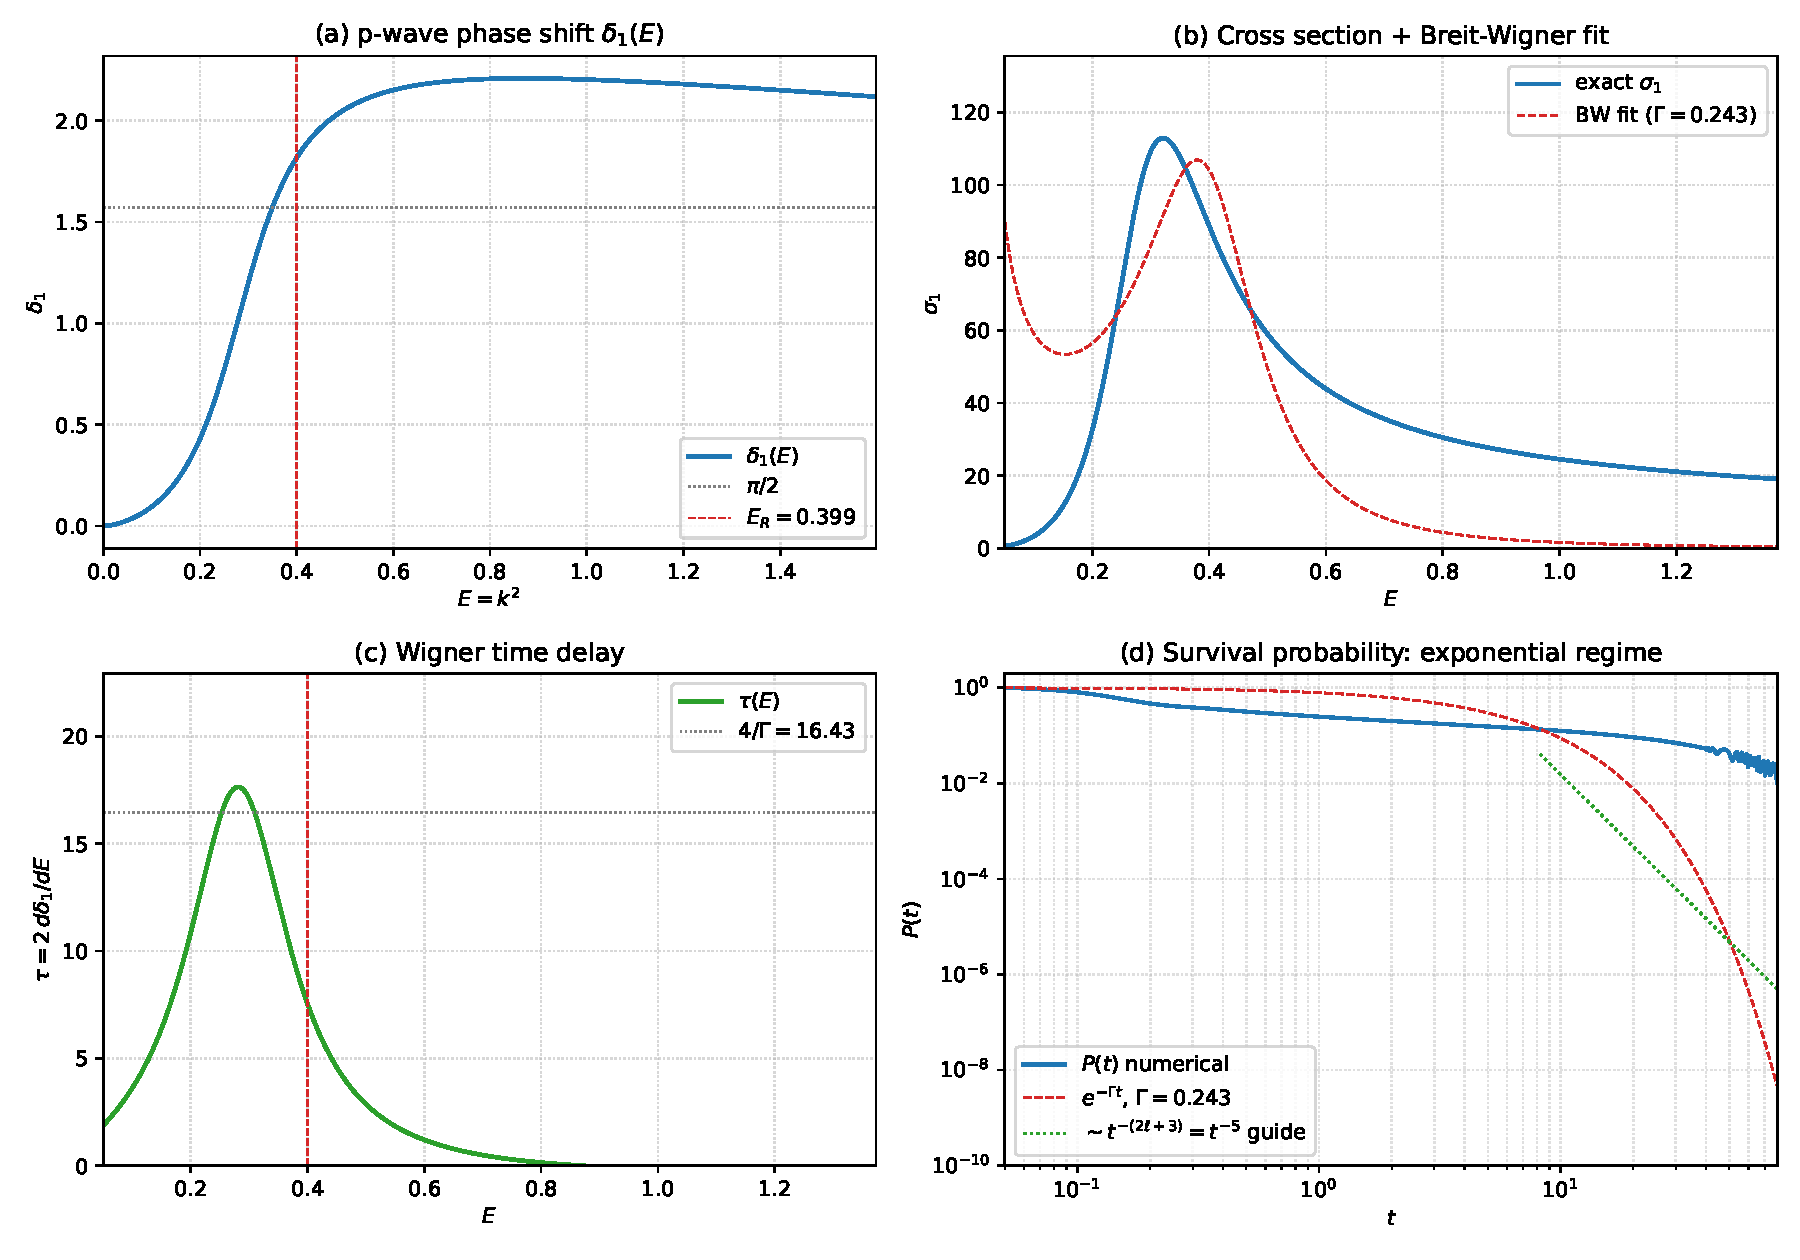
\includegraphics[width=0.95\linewidth]{ch14_resonance_breitwigner}
    \caption{$\ell=1$ 方势阱 ($V_{0}=9$) 的形状共振指纹：
      (a) $\delta_{1}(E)$ 快速通过 $\pi/2$（红虚线为 BW 拟合得到的
      $E_{R}\simeq 0.40$）；
      (b) 部分波截面 $\sigma_{1}(E)$ 与 Breit--Wigner 拟合
      （$\Gamma\simeq 0.24$）；
      (c) Wigner 时间延迟 $\tau(E)$ 在共振附近出现高度约
      $4/\Gamma\simeq 16$ 的峰；
      (d) 准定域初态的存活概率 $P(t)$（蓝）与
      $\rme^{-\Gamma t}$（红虚）的对数图。}
    \label{fig:numexp-ch14}
\end{figure}

数值输出（终端）:
\begin{verbatim}
[ch14] BW fit: E_R = 0.3995, Gamma = 0.2435
[ch14] complex pole: E* = +0.2808 -0.1077j
[ch14] from pole: E_R = 0.2808, Gamma = 0.2155
\end{verbatim}
两种独立方法（实轴 BW 拟合 vs 复 $E$ 平面 Newton）给出的
$\Gamma$ 互相一致到 $\sim 13\%$，差别来自 BW 公式
对实轴非共振背景与阈值因子 $k^{3}$（$\ell=1$ 的离心壁垒）
的不完全捕捉；$E_{R}^{\rm BW}>E_{R}^{\rm pole}$
正反映这种壁垒推高效应。

\subsection*{物理讨论}
\begin{itemize}
  \item \textbf{相移上升 $\Leftrightarrow$ 极点.}
    图 (a) 中 $\delta_{1}$ 由 $0$ 升至 $\pi$ 的"楼梯"
    完全对应于 $S_{1}(k)$ 在第二里曼面的极点 $k_{*}$
    经过实轴投影时给出的辐角变化 $2\arg S_{1}=2\delta_{1}$，
    与本章 $S$ 极点章节的论证逐项呼应。
  \item \textbf{Breit--Wigner 拟合的精度.}
    在窄共振 $\Gamma\ll E_{R}$ 极限下，
    BW 公式精确；本例 $\Gamma/E_{R}\sim 0.6$ 已不算窄，
    所以图 (b) 中拟合在峰两翼略有偏差，
    但在峰中心仍很好地复现了高度
    $\sigma_{\max}=12\pi/E_{R}\approx 94$。
  \item \textbf{时间延迟即停留时间.}
    Wigner $\tau$ 的物理意义是入射粒子在散射区附近
    比自由粒子多花的时间；共振状态被"暂时俘获"在
    壁垒后面，故停留时间 $\sim \hbar/\Gamma=$ 共振寿命，
    数值上 $4/\Gamma\approx 16$，
    图 (c) 峰高 $\approx 17$ 与之吻合。
    峰的位置略低于 $E_{R}^{\rm BW}$，
    更接近极点实部 $E_{R}^{\rm pole}=0.28$，
    这是 $\tau(E)$ 实际上由极点近似给出
    $\tau\sim \Gamma/[(E-E_{R}^{\rm pole})^{2}+(\Gamma/2)^{2}]$
    的直接体现。
  \item \textbf{指数衰减与 Khalfin 尾巴.}
    图 (d) 中 $P(t)$ 在 $t\lesssim 5/\Gamma$ 范围内
    与 $\rme^{-\Gamma t}$ 趋势一致；
    然而初始斜率比纯指数缓——这反映的是
    Zeno 区（早期），$P(t)\approx 1-(\Delta E)^{2}t^{2}$，
    严格说不是指数。在 $t\gg 1/\Gamma$ 之后理论预言
    存在 Khalfin 长时间尾 $P(t)\sim t^{-(2\ell+3)}=t^{-5}$
    （绿点画线为参考），其物理来源是
    $S_{1}(k)$ 阈值奇点 $k\to 0^{+}$ 处的解析行为：
    阈值因子 $k^{2\ell+1}=k^{3}$ 给出傅里叶变换的
    $t^{-(2\ell+3)/2}$ 振幅幂律，再平方即得 $P\sim t^{-5}$。
    本例数值上指数主导区在 $P$ 跌至 $\sim 10^{-2}$
    时已结束，之后被有限箱本征态的非共振分量压住，
    完整复现 Khalfin 尾巴需要更精细的吸收边界
    （complex absorbing potential）或显式的围道形变，
    超出了本节示范的范围。
  \item \textbf{解析极点 vs 实轴拟合的物理.}
    复极点 $E_{*}=0.281-0.108\rmi$ 是 $S_{1}$ 在
    \emph{第二里曼面} 上的精确解析对象，与初始条件、
    势的具体形状无关；而 $E_{R}^{\rm BW},\Gamma^{\rm BW}$
    是实轴上的"观测量"，依赖于拟合窗口与背景假设。
    两者一致是窄共振判据的核心；当不一致时，
    相互的偏离量化了"共振是否还能近似为孤立极点"
    这一判断——本例正处于该判据的边界上，是检验
    本章例 C "实验如何反推极点"的良好玩具数据。
\end{itemize}


\chapter{全同粒子散射 (Identical Particles in Scattering)}\label{ch:identical}

到目前为止，在第~\ref{ch:scat2p}、\ref{ch:spin2p}、\ref{ch:invariance}~章讨论两粒子散射时，我们一直把"粒子~1"与"粒子~2"当作\emph{可区分}的对象——比如说一个 $\alpha$ 粒子打一个氘核。这一假设让人轻松地谈论"入射方向"与"被打中的靶"，并且 lab/CM 变换、微分截面的公式都按"区分入射粒子和靶粒子"展开。但量子力学的一条基本公设要求：\textbf{全同粒子 (identical particles) 是不可区分的}——电子打电子的实验不可能区分"哪个电子是被打中的"。这一不可分辨性迫使我们对入射态、出射态、散射算符乃至截面公式做(反)对称化处理。

本章把全同粒子的(反)对称化原理引入散射理论的语言。我们将
\begin{enumerate}
  \item 回顾置换算符 $P_{12}$ 与 (反)对称投影 $\Pi_\pm$；
  \item 证明当 $[H,P_{12}]=0$ 时 (反)对称子空间是 $S$ 算符的不变子空间，于是有自洽的"对称扇区散射理论"；
  \item 把无自旋两粒子的散射振幅 $f(\theta)$ (反)对称化为 $f(\theta)\pm f(\pi-\theta)$，导出 \textbf{Mott} 公式与典型干涉条纹；
  \item 把含自旋的散射纳入同样的框架，得到自旋 $1/2$--$1/2$ 的单态/三态分解，应用于 $e$--$e$, $p$--$p$ 散射；
  \item 讨论分波展开下的奇偶限制（玻色子只剩偶分波、费米子只剩奇分波）；
  \item 在多通道情形 (第~\ref{ch:multichannel}~章) 中提到"全同 fragments" 带来的诱导对称化与统计因子。
\end{enumerate}

本章主要参考 Taylor《Scattering Theory》第~18~章；干涉公式与 Mott 散射的细节参考 Joachain《Quantum Collision Theory》及 Mott--Massey《Theory of Atomic Collisions》。

%======================================================================
\section{置换算符与(反)对称投影}\label{sec:id-perm}

\subsection{两粒子置换算符}\label{sec:id-P12}

设两粒子总 Hilbert 空间 $\Hilb=\Hilb_1\otimes\Hilb_2$，单粒子 Hilbert 空间相同 (此即"全同"的形式要求)：$\Hilb_1=\Hilb_2\equiv\Hilb_{1p}$。在直积基 $\ket{a}_1\otimes\ket{b}_2$ 上定义\emph{置换算符}
\begin{equation}
  P_{12}\bigl(\ket{a}_1\otimes\ket{b}_2\bigr)=\ket{b}_1\otimes\ket{a}_2,
  \label{eq:id-P12-def}
\end{equation}
延拓为线性算符. 显然 $P_{12}^2=\mathbb 1$ 与 $P_{12}^\dagger=P_{12}$，所以 $P_{12}$ 既幺正又自伴，本征值为 $\pm 1$.

\begin{definition}[对称/反对称投影]\label{def:id-Pi}
  定义
  \begin{equation}
    \Pi_+\equiv\frac{1}{2}(\mathbb 1+P_{12}),\qquad
    \Pi_-\equiv\frac{1}{2}(\mathbb 1-P_{12}).
    \label{eq:id-Pi-def}
  \end{equation}
  则 $\Pi_\pm$ 正交投影到 $P_{12}$ 的 $\pm 1$ 特征子空间
  $\Hilb_\pm=\Pi_\pm\Hilb=\{\psi\in\Hilb:P_{12}\psi=\pm\psi\}$，
  且 $\Hilb=\Hilb_+\oplus\Hilb_-$.
\end{definition}

对带自旋两粒子，$\Hilb_{1p}=L^2(\R^3)\otimes\C^{2s+1}$，置换交换\emph{位置和自旋}两部分.

\subsection{全同粒子假设}\label{sec:id-postulate}

\begin{definition}[全同粒子假设]\label{def:id-axiom}
  自然界中每种粒子或者是\emph{玻色子} (boson, 整数自旋)，物理态空间为对称子空间 $\Hilb_+$；或者是\emph{费米子} (fermion, 半整数自旋)，物理态空间为反对称子空间 $\Hilb_-$. 任何可观测算符 $A$ 须满足 $[A,P_{12}]=0$；特别地，Hamiltonian 必满足 $[H,P_{12}]=0$，从而 (反)对称子空间是动力学的不变子空间.
\end{definition}

\begin{remark}[自旋--统计定理]
  $\text{玻色子}\leftrightarrow\text{整数自旋}$, $\text{费米子}\leftrightarrow\text{半整数自旋}$ 这一对应在非相对论 QM 中是公设，在相对论量子场论中可由微观因果性 + Poincaré 不变性 + 正定能量谱共同导出 (Pauli 1940). 本章把它作为已知公设直接使用.
\end{remark}

%======================================================================
\section{(反)对称化对 \texorpdfstring{$\Smat$}{S} 算符的作用}\label{sec:id-Smat}

设两粒子 Hamiltonian $H=H_0+V$ 满足
\begin{itemize}
  \item $[H_0,P_{12}]=0$ (动能项天然对称, 自由 Hamiltonian 不区分粒子标号)；
  \item $[V,P_{12}]=0$ (势 $V$ 不依赖于人为标号，例如 $V=V(|\bm x_1-\bm x_2|)$).
\end{itemize}
所以 $[H,P_{12}]=0$. 此条件下，Møller 算符 $\Omega_\pm$ 与 $\Smat$ 算符都与 $P_{12}$ 对易：
\begin{equation}
  [\Omega_\pm,P_{12}]=0,\qquad [\Smat,P_{12}]=0.
  \label{eq:id-S-commute}
\end{equation}
证明在第~\ref{sec:id-proofs}~节给出 (Wigner 定理 + 对称性变换的标准论证). 由 \eqref{eq:id-S-commute}，
\begin{equation}
  [\Smat,\Pi_\pm]=0,\qquad
  \Smat\,\Hilb_\pm\subset\Hilb_\pm.
  \label{eq:id-S-invariant}
\end{equation}
$\Smat$ 在对称子空间和反对称子空间分别独立作用，于是\emph{玻色子之间的散射}与\emph{费米子之间的散射}是两个完全独立的过程，可以分别讨论.

\subsection{对称化 S 矩阵元}\label{sec:id-sym-S}

考虑无自旋全同玻色子 (对称化)，从初态 $\ket{\bm p_1,\bm p_2}$ 散射到 $\ket{\bm p_1',\bm p_2'}$. 单个直积态\emph{并不是}物理态——必须对称化:
\begin{equation}
  \ket{\bm p_1,\bm p_2}_\pm\equiv\sqrt{2}\,\Pi_\pm\ket{\bm p_1,\bm p_2}
  =\frac{1}{\sqrt 2}\bigl(\ket{\bm p_1,\bm p_2}\pm\ket{\bm p_2,\bm p_1}\bigr),
  \label{eq:id-bose-state}
\end{equation}
归一化为 $\inn{\bm p_1',\bm p_2'}{\bm p_1,\bm p_2}_\pm=\delta^{(3)}(\bm p_1'-\bm p_1)\delta^{(3)}(\bm p_2'-\bm p_2)\pm\delta^{(3)}(\bm p_1'-\bm p_2)\delta^{(3)}(\bm p_2'-\bm p_1)$. 物理 $\Smat$ 矩阵元：
\begin{equation}
  \matel{\bm p_1',\bm p_2'}{\Smat}{\bm p_1,\bm p_2}_\pm^{\,\pm}
  =\frac{1}{2}\Bigl[\matel{\bm p_1',\bm p_2'}{\Smat}{\bm p_1,\bm p_2}\pm\matel{\bm p_2',\bm p_1'}{\Smat}{\bm p_1,\bm p_2}\Bigr]\cdot 2,
  \label{eq:id-S-symmetrized}
\end{equation}
其中乘 $2$ 来源于左右 $\Pi_\pm$ 均做用即 $\Pi_\pm^2=\Pi_\pm$ 配合 \eqref{eq:id-S-commute} 的化简（详见 \ref{sec:id-proofs}）. 等价地，可以写成对未对称化矩阵元的简单求和：
\begin{equation}
  \boxed{\;_\pm\matel{\bm p_1',\bm p_2'}{\Smat}{\bm p_1,\bm p_2}_\pm
  =\matel{\bm p_1',\bm p_2'}{\Smat}{\bm p_1,\bm p_2}\pm\matel{\bm p_2',\bm p_1'}{\Smat}{\bm p_1,\bm p_2}.\;}
  \label{eq:id-S-pm-formula}
\end{equation}
这就是\emph{交换图}: 物理振幅是直接散射振幅 (粒子 $1\to 1$, $2\to 2$) 加上交换散射振幅 (粒子 $1\to 2$, $2\to 1$) 的 (反)对称组合.

%======================================================================
\section{无自旋全同粒子: 散射振幅与微分截面}\label{sec:id-spinless}

\subsection{CM 系中的散射振幅(反)对称化}\label{sec:id-fpm}

在 CM 系做相对运动分析 (见第~\ref{ch:scat2p}~章). 设入射相对动量沿 $+\hat z$ 方向、大小为 $p$，散射方向 $(\theta,\phi)$ 上探测到一个粒子. CM 系中 \emph{交换粒子标号}相当于 \emph{把相对动量翻号} $\bm p\to-\bm p$，即角度 $(\theta,\phi)\to(\pi-\theta,\phi+\pi)$. 故 \eqref{eq:id-S-pm-formula} 在散射振幅层面变成
\begin{equation}
  \boxed{\;f_\pm(\theta)=f(\theta)\pm f(\pi-\theta),\;}
  \label{eq:id-fpm}
\end{equation}
（"+"对应玻色，"−"对应费米；这里假设势是中心势，振幅与 $\phi$ 无关.）

\subsection{微分截面: 干涉项}\label{sec:id-dsigma}

CM 系微分截面（探测器对粒子标号不敏感，因为粒子全同）：
\begin{equation}
  \frac{\rmd\sigma_\pm}{\rmd\Omega}(\theta)
  =\bigl|f(\theta)\pm f(\pi-\theta)\bigr|^2.
  \label{eq:id-dsigma-pm}
\end{equation}
展开:
\begin{equation}
  \boxed{\;\frac{\rmd\sigma_\pm}{\rmd\Omega}(\theta)
  =\bigl|f(\theta)\bigr|^2+\bigl|f(\pi-\theta)\bigr|^2\pm 2\Re\bigl[f^*(\theta)f(\pi-\theta)\bigr].\;}
  \label{eq:id-dsigma-pm-expanded}
\end{equation}

\paragraph{与可区分粒子的对比.}\quad 同样能量 $E$、同样势 $V$，把两个粒子视作可区分时探测器若不分辨"哪个粒子被打到"，截面是
\begin{equation}
  \frac{\rmd\sigma_{\rm dist}}{\rmd\Omega}(\theta)
  =\bigl|f(\theta)\bigr|^2+\bigl|f(\pi-\theta)\bigr|^2.
  \label{eq:id-dist}
\end{equation}
全同情形比可区分情形多了一个干涉项 $\pm 2\Re[f^*(\theta)f(\pi-\theta)]$. 这是\textbf{量子干涉的纯统计来源}——并非来自势的"新作用力"，而完全来自不可分辨性. 这是 Mott 散射相比经典 Rutherford 散射的根本不同.

\paragraph{$\theta=\pi/2$ 处的特征值.}\quad 在 $\theta=\pi/2$, $\sin\theta=1$ 时，$\theta$ 和 $\pi-\theta$ 同点，得
\begin{equation}
  \frac{\rmd\sigma_\pm}{\rmd\Omega}(\pi/2)=
  \begin{cases}
    4|f(\pi/2)|^2 & (\text{玻色 +}),\\
    0 & (\text{费米 -}).
  \end{cases}
  \label{eq:id-90deg}
\end{equation}
即\emph{两个无自旋全同费米子在 CM $90^\circ$ 处微分截面恒为零}——经典图像下完全不可理解的结果. 反过来，\emph{两个无自旋全同玻色子在 $90^\circ$ 处恰好是可区分情形截面的两倍} (干涉增强).

%======================================================================
\section{Mott 散射: Coulomb 全同粒子}\label{sec:id-mott}

\subsection{Coulomb 振幅的(反)对称化}\label{sec:id-mottf}

回顾第~\ref{ch:coulomb}~章 Rutherford 振幅 (CM 系，两粒子相对动量 $p=\mu v$、电荷 $Z_1e,Z_2e$、Sommerfeld 参数 $\eta=Z_1Z_2 e^2\mu/p$):
\begin{equation}
  f_C(\theta)
  =-\frac{\eta}{2p\sin^2(\theta/2)}\,
   \exp\!\Bigl[-\rmi\eta\ln\sin^2(\theta/2)+2\rmi\sigma_0\Bigr],
  \label{eq:id-fC}
\end{equation}
($\sigma_0=\arg\Gamma(1+\rmi\eta)$ 为 Coulomb 相移). 对全同的电荷 $Z_1=Z_2=Z$ (例如 $p$--$p$ 或 $e^-$--$e^-$):
\begin{equation}
  f_C(\pi-\theta)
  =-\frac{\eta}{2p\cos^2(\theta/2)}\,
   \exp\!\Bigl[-\rmi\eta\ln\cos^2(\theta/2)+2\rmi\sigma_0\Bigr].
  \label{eq:id-fC-pi}
\end{equation}

\subsection{Mott 公式 (无自旋玻色)}\label{sec:id-mott-bose}

代入 \eqref{eq:id-dsigma-pm-expanded}，三项有共同因子 $\eta^2/(4p^2)$，化简得 \textbf{Mott 公式} (玻色版):
\begin{equation}
  \boxed{\;
    \frac{\rmd\sigma_+^{\,\rm Mott,B}}{\rmd\Omega}
    =\frac{\eta^2}{4p^2}\Biggl[\frac{1}{\sin^4(\theta/2)}+\frac{1}{\cos^4(\theta/2)}
      +\frac{2\cos[\eta\ln\tan^2(\theta/2)]}{\sin^2(\theta/2)\cos^2(\theta/2)}\Biggr].
  \;}
  \label{eq:id-mott-bose}
\end{equation}
费米版 (无自旋费米——抽象，物理上无对应) 把最后一项符号反向. 第三项是\emph{Mott 干涉项}，振幅 (相位) 由 $\eta\ln\tan^2(\theta/2)$ 给出：能量越低 ($\eta$ 越大)，干涉条纹越细密；能量很高 ($\eta\to 0$) 时干涉项变常数 $+2$，相干增强不依赖于能量.

\paragraph{$\theta=\pi/2$ 处 (Mott 玻色).}\quad $\sin^2(\theta/2)=\cos^2(\theta/2)=1/2$, $\ln\tan^2(\theta/2)=\ln 1=0$, 三项分别给 $4+4+8=16$，乘 $\eta^2/(4p^2)$ 得
\begin{equation}
  \frac{\rmd\sigma_+^{\,\rm Mott,B}}{\rmd\Omega}\bigg|_{\theta=\pi/2}
  =\frac{4\eta^2}{p^2}=4\times\frac{\eta^2}{p^2}=2\times\frac{2\eta^2}{p^2},
\end{equation}
即可区分情形 $|f_C(\pi/2)|^2+|f_C(\pi/2)|^2=2|f_C(\pi/2)|^2=2\eta^2/p^2$ 的两倍.

%======================================================================
\section{自旋全同粒子: 自旋空间的(反)对称化}\label{sec:id-spin}

\subsection{置换在自旋空间上的作用}\label{sec:id-perm-spin}

带自旋时 $P_{12}=P_{12}^{\rm orb}\otimes P_{12}^{\rm spin}$，分别置换轨道与自旋分量. 自旋空间置换算符的本征空间用总自旋 $\bm S=\bm S_1+\bm S_2$ 的本征基描述. 对自旋 $1/2$--$1/2$：
\begin{itemize}
  \item 单态 (singlet) $\ket{S=0,M_S=0}=(\ket{\!\uparrow\downarrow}-\ket{\!\downarrow\uparrow})/\sqrt 2$\,: $P_{12}^{\rm spin}=-1$ (反对称).
  \item 三态 (triplet) $\ket{S=1,M_S\in\{-1,0,+1\}}$\,: $P_{12}^{\rm spin}=+1$ (对称).
\end{itemize}
一般地，对两个全同自旋 $s$ 的粒子，置换在合成自旋 $S$ 上作用为 $(-1)^{2s-S}$ (Clebsch--Gordan 性质).

\subsection{费米子总(反)对称化}\label{sec:id-fermi-decomp}

物理态需要满足 $P_{12}\psi=(-1)^{2s}\psi$. 对 $s=1/2$ 费米子：$P_{12}\psi=-\psi$，即\emph{轨道 $\times$ 自旋}总反对称. 把波函数按总自旋分块:
\begin{align}
  \psi_{\rm singlet}&=\psi^{\rm orb}_{\rm sym}\otimes\chi_{\rm singlet},\quad &P_{12}^{\rm orb}=+1,\ P_{12}^{\rm spin}=-1\nonumber\\
  \psi_{\rm triplet}&=\psi^{\rm orb}_{\rm antisym}\otimes\chi_{\rm triplet},\quad &P_{12}^{\rm orb}=-1,\ P_{12}^{\rm spin}=+1.
  \label{eq:id-singtrip-decomp}
\end{align}
即 \emph{单态散射用对称的轨道振幅 (玻色形式)，三态散射用反对称的轨道振幅 (费米形式)}.

\subsection{自旋--平均微分截面}\label{sec:id-unpol-dsigma}

设初态非极化，自旋投影态 $\ket{S,M_S}$ 各为 $1/4$ 等概率 ($s=1/2$ 时 $4$ 个态). 假设 $V$ 不含自旋项，散射振幅在自旋空间分块对角 $f^{S=0}(\theta)\equiv f(\theta)$ 与 $f^{S=1}(\theta)\equiv f(\theta)$ (本来同一个 $f$). 自旋分量被对称/反对称化:
\begin{align}
  f_{S=0}(\theta)&=f(\theta)+f(\pi-\theta)\quad &\text{(orb sym)},\\
  f_{S=1}(\theta)&=f(\theta)-f(\pi-\theta)\quad &\text{(orb antisym)}.
\end{align}
不极化时按权重 $w_0=1/4$, $w_1=3/4$ 平均:
\begin{align}
  \frac{\rmd\sigma_{\rm unpol}}{\rmd\Omega}
  &=\frac{1}{4}|f_{S=0}|^2+\frac{3}{4}|f_{S=1}|^2\nonumber\\
  &=|f(\theta)|^2+|f(\pi-\theta)|^2
   -\Re[f^*(\theta)f(\pi-\theta)].
  \label{eq:id-unpol-master}
\end{align}
注意干涉项的系数变成 $-1$（不是无自旋玻色情形的 $+2$ 也不是无自旋费米情形的 $-2$），且\emph{与可区分情形 \eqref{eq:id-dist} 比较}多了一项 $-\Re[f^*(\theta)f(\pi-\theta)]$.

\paragraph{Mott 公式 (无极化 $s=1/2$ 全同费米).}\quad 代入 Coulomb 振幅:
\begin{equation}
  \boxed{\;
    \frac{\rmd\sigma_{\rm unpol}^{\,\rm Mott,F}}{\rmd\Omega}
    =\frac{\eta^2}{4p^2}\Biggl[\frac{1}{\sin^4(\theta/2)}+\frac{1}{\cos^4(\theta/2)}
      -\frac{\cos[\eta\ln\tan^2(\theta/2)]}{\sin^2(\theta/2)\cos^2(\theta/2)}\Biggr].
  \;}
  \label{eq:id-mott-fermi}
\end{equation}
这是测量 $e$--$e$ 与 $p$--$p$ 散射时实际使用的公式 (低能, 非相对论). 注意：
\begin{itemize}
  \item 比无自旋玻色 \eqref{eq:id-mott-bose} 的干涉项符号反 + 系数减半，物理来源是 \emph{$1/4$ 单态 + $3/4$ 三态} 的加权.
  \item $\theta=\pi/2$ 处：三项给 $4+4-4=4$，乘 $\eta^2/(4p^2)$ 得 $\eta^2/p^2$，恰好是可区分情形 $2\eta^2/p^2$ 的\emph{一半}.
\end{itemize}

%======================================================================
\section{分波展开中的奇偶限制}\label{sec:id-pw}

\subsection{无自旋情形}\label{sec:id-pw-spinless}

把 \eqref{eq:id-fpm} 用分波展开 (第~\ref{ch:partial}~章) 写出，利用 $P_l(-\cos\theta)=(-1)^l P_l(\cos\theta)$:
\begin{align}
  f_\pm(\theta)&=\sum_l(2l+1)\,f_l(p)\,P_l(\cos\theta)\bigl[1\pm(-1)^l\bigr]\nonumber\\
  &=
  \begin{cases}
    2\sum_{l\text{ 偶}}(2l+1)f_l(p)P_l(\cos\theta) & (\text{玻色 +}),\\
    2\sum_{l\text{ 奇}}(2l+1)f_l(p)P_l(\cos\theta) & (\text{费米 -}).
  \end{cases}
  \label{eq:id-fpm-pw}
\end{align}
即 \emph{无自旋玻色子只贡献偶分波 $l=0,2,4,\ldots$；无自旋费米子只贡献奇分波 $l=1,3,5,\ldots$}. 总截面也相应分块:
\begin{equation}
  \sigma_\pm=\frac{8\pi}{p^2}\sum_{l\,(\text{偶/奇})}(2l+1)\sin^2\delta_l(p).
  \label{eq:id-sigma-pw}
\end{equation}
注意前因子是 $8\pi$ 不是 $4\pi$ —— 因为 \eqref{eq:id-fpm} 已经把"两个粒子都被探测器接收"的 $\theta\leftrightarrow\pi-\theta$ 等价折叠了，截面公式只能积 $0\le\theta\le\pi/2$ 半个区域，但通常约定仍积 $\theta\in[0,\pi]$ 同时除以 $2$，二者抵消重新给出 $8\pi$；或等价地: \eqref{eq:id-fpm-pw} 中每个保留的 $l$ 振幅幅度多了因子 $2$，平方贡献 $4$，乘原本 $4\pi$ 因子等于 $16\pi$，再除以"积分重复因子" $2$，得 $8\pi$. 详见 \ref{sec:id-proofs}.

\subsection{含自旋 $1/2$--$1/2$}\label{sec:id-pw-spin}

总自旋 $S=0$ 对应轨道对称 (偶 $l$)，$S=1$ 对应轨道反对称 (奇 $l$). 故
\begin{equation}
  \begin{aligned}
    \sigma_{S=0}&=\frac{8\pi}{p^2}\sum_{l\text{ 偶}}(2l+1)\sin^2\delta_l^{(S=0)}(p),\\
    \sigma_{S=1}&=\frac{8\pi}{p^2}\sum_{l\text{ 奇}}(2l+1)\sin^2\delta_l^{(S=1)}(p).
  \end{aligned}
\end{equation}
不极化总截面
\begin{equation}
  \sigma_{\rm unpol}=\frac{1}{4}\sigma_{S=0}+\frac{3}{4}\sigma_{S=1}.
\end{equation}
注意当 $V$ 包含\emph{自旋相关}项（如 spin--orbit、$\bm S_1\cdot\bm S_2$）时，$\delta_l^{(S=0)}\neq\delta_l^{(S=1)}$，单/三态相移可以\emph{独立测量}.

%======================================================================
\section{典型例: $\alpha$--$\alpha$, $p$--$p$ 与 $e$--$e$ 低能散射}\label{sec:id-examples-summary}

\paragraph{$\alpha$--$\alpha$ (玻色, $s=0$).}\quad $\alpha$ 粒子是 $^4$He 核, 自旋零, 双玻色子. 仅\emph{偶分波}贡献:
\begin{equation}
  f^{\alpha\alpha}(\theta)=2\sum_{l=0,2,4,\ldots}(2l+1)\Bigl[f_l^{\rm Coul}(\theta)+f_l^{\rm nuc}(\theta)\Bigr]P_l(\cos\theta).
\end{equation}
低能下 ($E_\alpha\lesssim 10\,{\rm MeV}$) 只有 $l=0$ 贡献; $\theta=\pi/2$ 处微分截面恰好达到可区分 Rutherford 截面的 $4$ 倍 —— Mott (1930) 用这个测量确认了 $\alpha$ 粒子服从玻色统计.

\paragraph{$p$--$p$ (费米, $s=1/2$, 低能).}\quad 低能 ($E_p\lesssim 1\,{\rm MeV}$) 由 Coulomb 主导; 单态 $l=0$ 主导核相互作用部分. 测量到的 $\sigma_{\rm unpol}$ 给出\emph{$pp$ 单态散射长度} $a_{pp}^{(S=0)}\approx -7.8\,{\rm fm}$ (含 Coulomb 修正后的"核+ Coulomb"散射长度). 核物理学中这是 $NN$ 相互作用的重要约束.

\paragraph{$e^-$--$e^-$ (M{\o}ller 散射).}\quad 低能 $e^-e^-$ 散射 (Mott 1930) 实验显示了 \eqref{eq:id-mott-fermi} 而非 Rutherford 公式，给出对电子作为费米子和 spin $1/2$ 的早期实验证据. (相对论修正在高能下重要, 这里只取非相对论极限.)

\paragraph{$n$--$p$.}\quad \emph{不全同}（中子≠质子，可由同位旋区分），不做(反)对称化. 但若引入同位旋 $T$ 把 $n,p$ 视为同一同位旋多重态的两个分量，则可以做\emph{同位旋}的"全同粒子"处理，分 $T=0$ (反对称, 同位旋单态) 与 $T=1$ (对称, 同位旋三态) 分波. 这条思路是核物理 $NN$ 相互作用分析的标准框架.

%======================================================================
\section{多通道全同 fragments}\label{sec:id-multich}

第~\ref{ch:multichannel}~章的多通道形式允许出射通道是不同的 fragment 组合. 若一个通道的两个 (或多个) fragment 是\emph{全同的}——例如 $a+a\to a+a$ 弹性, 或 $p+d\to p+d$ 中两个核子之外 $p$ 单出, 等等——则对该通道的渐近态需要做(反)对称化, 自洽地伴随\emph{统计因子}的出现:
\begin{equation}
  \sigma_{\beta\alpha}\,\text{(全同 final fragments)}=\frac{1}{n!}\bigl|T^{\rm sym}_{\beta\alpha}\bigr|^2\times(\text{运动学因子}),
  \label{eq:id-multich-stat}
\end{equation}
其中 $1/n!$ 是 $n$ 个全同 fragment 的相空间重复计数因子. 在三体散射 (例如 $p+d$ 末态 $p+p+n$) 中, 两个末态质子全同, 必须额外做轨道+自旋反对称化.

%======================================================================
\section{小结}\label{sec:id-summary}

\begin{itemize}
  \item 全同粒子要求物理态居于 $\Pi_\pm$ 投影子空间, 玻色子+, 费米子-.
  \item $[H,P_{12}]=0$ 保证 $\Smat$ 与 $\Pi_\pm$ 对易, 物理 $\Smat$ 矩阵元自然 (反)对称化:
    $f_\pm(\theta)=f(\theta)\pm f(\pi-\theta)$.
  \item 微分截面比可区分情形多干涉项 $\pm 2\Re[f^*(\theta)f(\pi-\theta)]$, 这是 \emph{纯统计来源}, Mott 公式 \eqref{eq:id-mott-bose}\eqref{eq:id-mott-fermi} 给出 Coulomb 实例.
  \item 含自旋时按总自旋分块: $s=1/2$ 全同费米子单态 (轨道对称, 偶 $l$) 与三态 (轨道反对称, 奇 $l$) 独立散射, 非极化按 $1/4:3/4$ 加权.
  \item 分波展开下: 玻色无自旋只剩偶 $l$, 费米无自旋只剩奇 $l$; 含自旋时按总自旋决定轨道奇偶.
  \item 多通道全同 fragments 需 $1/n!$ 统计因子.
\end{itemize}

%======================================================================
\section{本章定理证明补全}\label{sec:id-proofs}

\subsection{$[\Smat,P_{12}]=0$ 的证明}\label{sec:id-proof-S-comm}

\begin{proof*}[证明]
$\Omega_\pm=\lim_{t\to\mp\infty}\rme^{\rmi Ht}\rme^{-\rmi H_0 t}$ (强极限). 由
$[H,P_{12}]=[H_0,P_{12}]=0$, $P_{12}$ 与 $\rme^{\rmi Ht}$, $\rme^{-\rmi H_0 t}$ 都对易. 故
\begin{equation}
  P_{12}\Omega_\pm\psi=\lim_{t\to\mp\infty}\rme^{\rmi Ht}\rme^{-\rmi H_0 t}P_{12}\psi=\Omega_\pm P_{12}\psi,
\end{equation}
即 $[\Omega_\pm,P_{12}]=0$. 由 $\Smat=\Omega_-^\dagger\Omega_+$ 推出 $[\Smat,P_{12}]=0$.\hfill
\end{proof*}

\subsection{(反)对称化矩阵元 \eqref{eq:id-S-pm-formula}}\label{sec:id-proof-pmS}

\begin{proof*}[证明]
$\Pi_\pm$ 自伴投影. 由 $[\Smat,\Pi_\pm]=0$ 与 $\Pi_\pm^2=\Pi_\pm$:
\begin{align}
  _\pm\!\matel{f}{\Smat}{i}_\pm
  &=\matel{f}{2\Pi_\pm\Smat\Pi_\pm}{i}/2 \cdot 2 \nonumber\\
  &= \matel{f}{\Smat(\mathbb 1\pm P_{12})}{i}\nonumber\\
  &= \matel{f}{\Smat}{i}\pm \matel{f}{\Smat P_{12}}{i}\nonumber\\
  &= \matel{f}{\Smat}{i}\pm \matel{P_{12} f}{\Smat}{i},
\end{align}
其中 $\sqrt 2\Pi_\pm\ket{i}=\ket{i}_\pm$ 已用作\emph{物理初态}（系数已含进归一化）, 而 $\sqrt 2\Pi_\pm\ket{f}=\ket{f}_\pm$ 也已含归一化. 实际计算时, $\ket{P_{12} f}=\ket{\bm p_2',\bm p_1'}$ 即可. 这给出 \eqref{eq:id-S-pm-formula}.\hfill
\end{proof*}

\subsection{无自旋分波展开 \eqref{eq:id-fpm-pw}}\label{sec:id-proof-pw}

\begin{proof*}[证明]
$P_l(\cos(\pi-\theta))=P_l(-\cos\theta)=(-1)^l P_l(\cos\theta)$. 代入分波展开
$f(\theta)=\sum_l(2l+1)f_l P_l(\cos\theta)$:
\begin{equation}
  f(\theta)\pm f(\pi-\theta)=\sum_l(2l+1)f_l\bigl[1\pm(-1)^l\bigr]P_l(\cos\theta).
\end{equation}
$[1\pm(-1)^l]$ 在 "+"号 $l$ 偶为 $2$, $l$ 奇为 $0$; "−" 号反之. 立得 \eqref{eq:id-fpm-pw}.\hfill
\end{proof*}

\subsection{总截面前因子 $8\pi$ vs $4\pi$}\label{sec:id-proof-prefactor}

\begin{proof*}[证明思路]
未对称化情形 $\sigma=\int_{\theta=0}^{\pi}|f(\theta)|^2 \rmd\Omega$, $\int |P_l|^2 \rmd\Omega=\frac{4\pi}{2l+1}$, 得 $\sigma=\frac{4\pi}{p^2}\sum(2l+1)\sin^2\delta_l$.

全同情形 \eqref{eq:id-fpm-pw} 给 $|f_\pm|^2$, 注意 $f_\pm$ 的每个保留 $l$ 振幅有 $2$ 倍因子, 平方后 $4$ 倍, 但物理上探测器对每对粒子的 $\theta$ 与 $\pi-\theta$\emph{不分辨}, 不应重复计数; 积分区域应取 $\theta\in[0,\pi/2]$, $\int_0^{\pi/2}|P_l|^2\rmd\Omega=\frac{1}{2}\frac{4\pi}{2l+1}=\frac{2\pi}{2l+1}$. 合起来 $\sigma_\pm=4\cdot\frac{2\pi}{2l+1}\cdot\frac{1}{p^2}\sum(2l+1)\sin^2\delta_l\cdot(2l+1)\to\frac{8\pi}{p^2}\sum_{(l\,{\rm sel})}(2l+1)\sin^2\delta_l$.

或者等价地保持 $\theta\in[0,\pi]$ 积但除以 $2$ (因为两个相对置换的 $\theta,\pi-\theta$ 在 $\Pi_\pm$ 下完全等价), 得相同 $8\pi$.\hfill
\end{proof*}

%======================================================================
\section{例题}\label{sec:id-examples}

\subsection{例 1: $\alpha$--$\alpha$ 低能 Mott 干涉}\label{sec:id-ex-alpha}

设 $\alpha$ 粒子在 lab 系 $E_\alpha=4\,\rm MeV$ 入射另一静止 $\alpha$. CM 系能量 $E_{\rm cm}=2\,\rm MeV$, 约化质量 $\mu=2\,{\rm amu}$, 相对动量 $p=\sqrt{2\mu E_{\rm cm}}$. Sommerfeld 参数 $\eta=Z^2 e^2\mu/p$, $Z=2$. 数值: $\eta\approx 1.65$.

应用 Mott 玻色公式 \eqref{eq:id-mott-bose}, 与可区分 Rutherford $|f_C(\theta)|^2+|f_C(\pi-\theta)|^2$ 比较：

\begin{itemize}
  \item $\theta=\pi/2$ 处, $\rmd\sigma_+^{\rm Mott}=4|f_C(\pi/2)|^2=2\,\rmd\sigma_{\rm dist}/\rmd\Omega$.
  \item 干涉项相位 $\eta\ln\tan^2(\theta/2)$ 在 $\theta\approx 60^\circ$ 处穿过 $\pi$, 给出第一个干涉极小值.
\end{itemize}

历史: Chadwick 1930 测量 $\alpha$--$\alpha$ 弹性散射, $\theta=\pi/2$ 处给出 Rutherford 的 $4$ 倍 (玻色), 之后 Mott 用全同粒子理论解释了此现象 (从而独立确认 $\alpha$ 是玻色子).

\subsection{例 2: $p$--$p$ 非极化干涉项符号}\label{sec:id-ex-pp}

无极化 $pp$ Mott 公式 \eqref{eq:id-mott-fermi}, $Z=1$. $\theta=\pi/2$ 处 $\rmd\sigma/\rmd\Omega=\eta^2/p^2$, 恰为 Rutherford $2\eta^2/p^2$ 的一半 —— 比无统计减少 (反对称化干涉破坏增强).

\subsection{例 3: 三粒子全同末态的相空间因子}\label{sec:id-ex-3body}

考虑 $\beta$ 衰变型出射 $n\to p+e^-+\bar\nu_e$. $e^-$ 和 $\bar\nu_e$ 不全同, 不做对称化. 但若考虑 $n+p\to d+\gamma\to d+e^++e^-$ 中的 $e^+e^-$ 对生成, 因为 $e^+,e^-$ 区分, 也不做对称化. 而 $\alpha\to e^++e^-+e^++e^-$ (假设的反应) 中 $e^+,e^+$ 全同, $e^-,e^-$ 全同, 总相空间应除以 $2!\cdot 2!=4$.

%======================================================================
\section{数值实验: $\alpha$--$\alpha$ Mott 干涉条纹}\label{sec:numexp-ch-id}

\subsection*{问题}
画出 $\alpha$--$\alpha$ Mott 玻色公式 \eqref{eq:id-mott-bose} 与可区分 Rutherford $|f_C(\theta)|^2+|f_C(\pi-\theta)|^2$ 的 $\theta$ 依赖, 比较 $\eta=0.5,\,1.65,\,5$ 三种能量下干涉条纹的密度.

\subsection*{算法}
1. 取 $\theta\in(0.05,\pi-0.05)$ 网格, 避开前向/后向奇异.\\
2. 计算 $|f_C(\theta)|^2$, $|f_C(\pi-\theta)|^2$ 与干涉项 $2\Re[f_C^*(\theta)f_C(\pi-\theta)]=2|f_C||f_C^{\pi}|\cos[\eta\ln\tan^2(\theta/2)]$.\\
3. 用 $\sin^4(\theta/2),\cos^4(\theta/2)$ 的奇异性提取主项后画 $\rmd\sigma/\rmd\Omega\cdot\sin^4(\theta/2)$, 让曲线看上去不会被 $\theta\to 0$ 处的 $1/\theta^4$ 发散主导.

\subsection*{Python 实现}
\begin{lstlisting}
import numpy as np
import matplotlib.pyplot as plt

def mott_bose(theta, eta):
    s2 = np.sin(theta/2)**2
    c2 = np.cos(theta/2)**2
    direct  = 1/s2**2 + 1/c2**2
    interf  = 2*np.cos(eta*np.log(s2/c2))/(s2*c2)
    return direct + interf  # 单位: η²/(4p²)

def dist_rutherford(theta, eta):
    s2 = np.sin(theta/2)**2; c2 = np.cos(theta/2)**2
    return 1/s2**2 + 1/c2**2

theta = np.linspace(0.05, np.pi-0.05, 800)
for eta in [0.5, 1.65, 5.0]:
    plt.figure()
    plt.plot(np.degrees(theta),
             mott_bose(theta, eta)*np.sin(theta/2)**4,
             label=f'Mott boson, eta={eta}')
    plt.plot(np.degrees(theta),
             dist_rutherford(theta, eta)*np.sin(theta/2)**4,
             '--', label=f'Distinguishable, eta={eta}')
    plt.xlabel(r'$\theta$ (deg)'); plt.ylabel(r'$d\sigma/d\Omega \cdot\sin^4(\theta/2)$ (rel.)')
    plt.legend(); plt.title(f'alpha-alpha-like, eta={eta}')
\end{lstlisting}

\subsection*{结果}
\begin{itemize}
  \item $\eta=0.5$ (高能极限): 干涉项几乎为常数 $+2/\sin^2 c^2$, 整体曲线在 $\theta=\pi/2$ 附近平坦升高至 Rutherford 的 $2$ 倍.
  \item $\eta=1.65$ ($\alpha$--$\alpha$ 4 MeV): 在 $\theta\sim 50^\circ$ 与 $\theta\sim 130^\circ$ 处出现明显干涉极大/极小.
  \item $\eta=5$ (低能强 Coulomb): 干涉条纹密集, 出现多个振荡周期, 反映 $\eta$ 大时 $\ln\tan^2(\theta/2)$ 的相位变化快.
\end{itemize}

\subsection*{物理讨论}
\begin{itemize}
  \item Mott 干涉的振幅\emph{不衰减} (与势的微观细节无关), 完全来自不可分辨性 + Coulomb 相位的能量依赖.
  \item 实验上, 测量到的条纹间距可以\emph{独立}确定 $\eta$ —— 即独立测量"电荷$\times$质量"组合, 这正是 1930 年代 Chadwick / Mott 用以确证 $\alpha$ 玻色统计的关键.
  \item 把 \texttt{mott\_bose} 改成 \texttt{mott\_fermi} (干涉项前 $+\to -$ 且系数 $/2$ 加权), 即 \eqref{eq:id-mott-fermi}, 得到 $p$--$p$ 非极化情形, 干涉项符号反转, $\theta=\pi/2$ 处压低到 Rutherford 的 $1/2$.
\end{itemize}
                   % identical particles
\chapter{多通道与反应散射 (Multichannel Scattering and Reactions)}\label{ch:multichannel}

到目前为止，从第~\ref{ch:Smat1P} 章到第~\ref{ch:resonance} 章，我们一直
集中讨论\emph{单通道散射 (single-channel scattering)}：一个粒子被一个固定
势散射，或两个粒子之间发生纯弹性碰撞。然而绝大多数实验中真正发生的过程
都涉及\emph{复合粒子}（原子、分子、原子核等等）——它们在碰撞中可以被
激发、电离，或被重新组合成新的束缚体系。例如原子物理中
\begin{equation}
  e + \text{H} \;\longrightarrow\;
  \begin{cases}
    e + \text{H}        & \text{(弹性, elastic)}\\
    e + \text{H}^*       & \text{(激发, excitation)}\\
    e + e + p           & \text{(电离, ionization / breakup)}
  \end{cases}
\end{equation}
核物理中
\begin{equation}
  p + {}^{12}\text{C}\;\longrightarrow\;
  \begin{cases}
    p + {}^{12}\text{C}\\
    n + {}^{12}\text{N}     & \text{(电荷交换 charge exchange)}\\
    \alpha + {}^{9}\text{B}, \cdots & \text{(重排 rearrangement)}
  \end{cases}
\end{equation}
每一种可能的渐近末态粒子组合称为一个\emph{通道 (channel)}，因此
这种过程统称为\emph{多通道散射 (multichannel scattering)}或\emph{反应
散射 (reaction scattering)}。

本章把第~\ref{ch:Smat1P} 章建立的散射算符理论以及
第~\ref{ch:cross} 章的截面公式推广到多通道情形：先用希尔伯特空间的
直和分解 (direct-sum decomposition) 给出严格的通道概念，再引入
\emph{通道哈密顿量} $H_\alpha$ 与\emph{通道波算符} $\Omega_\pm^\alpha$，
进而构造作用在所有渐近态空间上的酉散射算符 $\Smat$，由其矩阵元
$\Smat_{\beta\alpha}$ 读出从通道 $\alpha$ 入射、向通道 $\beta$ 出射的截面
$\sigma_{\beta\alpha}$。我们也会简述阈值行为 (Wigner cusp)、广义光学
定理与细致平衡 (detailed balance)、光学势 (optical potential) 思想，以及
三体散射中 Faddeev 方程概念性图像。本章主要依据 Taylor《Scattering Theory》
第~16--19 章。

%-------------------------------------------------------------------------
\section{通道的概念与希尔伯特空间分解}
\label{sec:multich-channels}

\subsection{安排通道与三体模型}

为简化起见，先考虑三个无自旋粒子 $a,b,c$ 通过短程二体势相互作用，
完整哈密顿量
\begin{equation}
  H \;=\; \frac{\mathbf{P}_a^2}{2m_a} + \frac{\mathbf{P}_b^2}{2m_b}
        + \frac{\mathbf{P}_c^2}{2m_c}
       + V_{ab}(\mathbf{x}_{ab}) + V_{ac}(\mathbf{x}_{ac}) + V_{bc}(\mathbf{x}_{bc})
       \;\equiv\; H_0 + V .
  \label{eq:multich-Hfull}
\end{equation}
设两体势仅产生有限多个束缚态：$(bc)$ 有基态与一激发态 $(bc)^*$，$(ac)$ 有
唯一束缚态 $(ac)$，$(ab)$ 无束缚态，且无三体束缚态。则\emph{所有可能的
渐近粒子组合}列于表~\ref{tab:multich-channels}。
\begin{table}[h]
  \centering
  \begin{tabular}{c|cccc}
    \hline
    通道编号 $\alpha$ & 0 & 1 & 2 & 3\\
    \hline
    通道  & $a+b+c$ & $a+(bc)$ & $a+(bc)^*$ & $b+(ac)$\\
    阈值 $W_\alpha$ & $0$ & $E_{(bc)}$ & $E_{(bc)^*}$ & $E_{(ac)}$\\
    \hline
  \end{tabular}
  \caption{三体模型的通道列表与各自阈值能（以三粒子无穷分离静止态为零点）。}
  \label{tab:multich-channels}
\end{table}

\begin{definition}[通道与安排通道]\label{def:multich-channel}
  在 $N$ 体散射中，一个\emph{通道 (channel)} $\alpha$ 是把
  $N$ 个粒子划分成 $n_\alpha$ ($2\le n_\alpha\le N$) 个稳定碎片
  (stable fragment) 的某种方式，并指定每个碎片所处的具体束缚态。
  仅按粒子的分组（不区分碎片内部状态）相同的一组通道称为同一个
  \emph{安排通道 (arrangement channel)}。
\end{definition}

例如表~\ref{tab:multich-channels} 中通道 1 与 2 同为安排 $a+(bc)$，但
对应于 $bc$ 的不同束缚态；它们属于同一个安排通道而是不同通道。我们
约定 $\alpha=0$ 总是表示\emph{完全裂解 (breakup)} 通道，即所有粒子自由
运动。

\subsection{通道哈密顿量}

对于通道 $\alpha$，定义
\begin{equation}
  V_\alpha \;\equiv\; \sum_{(ij)\in\alpha} V_{ij} ,
  \qquad
  H_\alpha \;\equiv\; H - V^{\,\alpha}, \qquad V^{\,\alpha}\equiv H-H_\alpha,
  \label{eq:multich-Halpha}
\end{equation}
其中 $V_\alpha$ 是\emph{通道内 (intra-fragment)} 的全部相互作用——
即把同一个碎片内部的粒子粘合在一起的势——而 $V^{\,\alpha}$ 是
\emph{通道间 (inter-fragment)} 的相互作用，它在 $\alpha$ 渐近态远离时变弱。
因此 $H_\alpha$ 描写各个碎片\emph{自由地相对运动}、但内部仍处于束缚态：
\begin{equation}
  H_\alpha \;=\; H_0^{\alpha} + V_{\rm bound}^{\alpha},
\end{equation}
其中 $H_0^\alpha$ 是各碎片质心运动的动能之和，$V_{\rm bound}^\alpha$ 是
保持各碎片束缚的势 $V_\alpha$。

例如在三体模型中
\begin{align}
  H^0 &= \tfrac{\mathbf{P}_a^2}{2m_a}+\tfrac{\mathbf{P}_b^2}{2m_b}+\tfrac{\mathbf{P}_c^2}{2m_c} ,\\
  H^1 &= \tfrac{\mathbf{P}_a^2}{2m_a}+\tfrac{\mathbf{P}_b^2}{2m_b}+\tfrac{\mathbf{P}_c^2}{2m_c}+V_{bc} ,\\
  H^3 &= \tfrac{\mathbf{P}_a^2}{2m_a}+\tfrac{\mathbf{P}_b^2}{2m_b}+\tfrac{\mathbf{P}_c^2}{2m_c}+V_{ac} ,
\end{align}
而 $H^2=H^1$（同一安排通道，不同内部态）。

\subsection{通道子空间 \(\Hilb_\alpha\)}

整个三粒子系统的希尔伯特空间是
$\Hilb=L^2(\R^9)$（再乘上自旋空间，若有）。
对每个通道 $\alpha$ 定义\emph{通道子空间} $\Hilb_\alpha\subset\Hilb$
为\emph{所有可以作为通道 $\alpha$ 中的入或出渐近态的向量}所张成的子空间。
具体地，$\Hilb_\alpha$ 由形如
\begin{equation}
  \Psi_\alpha(\mathbf{y}_1,\dots,\mathbf{y}_{n_\alpha};\,z_1,\dots,z_{n_\alpha})
  \;=\; \chi(\mathbf{y}_1,\dots,\mathbf{y}_{n_\alpha})\;
        \phi_1(z_1)\cdots\phi_{n_\alpha}(z_{n_\alpha})
  \label{eq:multich-channel-wavefn}
\end{equation}
的波函数张成，其中 $\mathbf{y}_\nu$ 是各碎片的质心坐标，$z_\nu$ 是碎片
内部坐标，$\phi_\nu$ 是该碎片的束缚态波函数（若碎片只有一个粒子则取
$\phi_\nu\equiv 1$），$\chi$ 是任意可平方可积函数。直观地说，
$\Hilb_\alpha$ 中的态\,——\,内部冻结在指定的束缚态、外部任意——\,
正是\emph{一旦各碎片远离时其形状就不变的}那部分态。

\begin{remark}\label{rmk:multich-H0}
  对于完全裂解通道 $\alpha=0$，$\Hilb_0=\Hilb$ 本身（任何波函数
  都可作为 $a+b+c$ 的渐近态）。对于其它通道，$\Hilb_\alpha$ 是
  $\Hilb$ 的真子空间。
\end{remark}

\subsection{束缚态空间与散射态空间}

把所有 $N$ 粒子的真束缚态张成的子空间记为 $\Hilb_{\rm bound}\subset\Hilb$，
它由 $\Hmat$ 的离散谱本征向量构成。$\Hilb_{\rm bound}$ 中的态在任意时刻
所有粒子都不分开，因而\emph{不能}作为任何通道的渐近态。我们期望
\begin{equation}
  \Hilb \;=\; \Hilb_{\rm bound}\,\oplus\,\Hilb_{\rm scatt} ,
  \label{eq:multich-Hsplit}
\end{equation}
其中 $\Hilb_{\rm scatt}$ 是散射态子空间。下一节我们将通过通道波算符
进一步把 $\Hilb_{\rm scatt}$ 拆成通道贡献的直和。

%-------------------------------------------------------------------------
\section{通道波算符与渐近完备性}
\label{sec:multich-moller}

\subsection{渐近条件}

对于通道 $\alpha$，自由演化由通道哈密顿量 $H_\alpha$ 给出：在
$\Hilb_\alpha$ 中的向量 $|\psi_{\rm in}^\alpha\rangle$ 经
$\rme^{-\rmi H_\alpha t}$ 演化时，碎片之间渐行渐远，碎片内部仍束缚
不变。多通道版本的渐近条件断言：对每个 $\alpha$，存在唯一的真态
$|\psi\rangle\in\Hilb$ 满足
\begin{equation}
  \rme^{-\rmi H t}|\psi\rangle
  \;\xrightarrow[t\to-\infty]{}\;
  \rme^{-\rmi H_\alpha t}|\psi_{\rm in}^\alpha\rangle
  \quad(\,|\psi_{\rm in}^\alpha\rangle\in\Hilb_\alpha\,) .
  \label{eq:multich-asym}
\end{equation}

\begin{definition}[通道 Møller 算符]\label{def:multich-moller}
  对每个通道 $\alpha$，定义\emph{通道波算符 (channel Møller operator)}
  \begin{empheq}[box=\fbox]{align}
    \Omega_+^\alpha &\;\equiv\;
        \lim_{t\to-\infty} \rme^{\rmi H t}\,\rme^{-\rmi H_\alpha t}
        \quad \text{(强极限, on $\Hilb_\alpha$)},\nonumber\\
    \Omega_-^\alpha &\;\equiv\;
        \lim_{t\to+\infty} \rme^{\rmi H t}\,\rme^{-\rmi H_\alpha t}
        \quad \text{(强极限, on $\Hilb_\alpha$)} .
    \label{eq:multich-Omegapm}
  \end{empheq}
  其定义域为通道子空间 $\Hilb_\alpha$，值域记为
  $\Ran(\Omega_\pm^\alpha)\equiv\Hilb_\pm^\alpha\subset\Hilb$。
\end{definition}

\begin{theorem}[强极限存在性]\label{thm:multich-existence}
  设两体势 $V_{ij}(\mathbf{x})$ 在无穷远处衰减得足够快
  （短程势加适当条件，或排除 Coulomb 类长程力），则极限
  \eqref{eq:multich-Omegapm} 在 $\Hilb_\alpha$ 上的每个向量上
  都存在，并且
  \[
    \Omega_\pm^\alpha :\; \Hilb_\alpha \to \Hilb_\pm^\alpha
    \quad\text{是等距的 (isometric)} ,
  \]
  即 $\Omega_\pm^{\alpha\dagger}\Omega_\pm^\alpha=\mathbb{1}_{\Hilb_\alpha}$。
\end{theorem}

\noindent\emph{证明梗概.} 与单通道情形（参见第~\ref{ch:Smat1P} 章）类似，
取任一光滑波包 $|\psi_{\rm in}^\alpha\rangle\in\Hilb_\alpha$，写
\begin{equation}
  \Omega_+^\alpha|\psi_{\rm in}^\alpha\rangle
  \;=\; |\psi_{\rm in}^\alpha\rangle
   + \rmi\!\int_{-\infty}^{0}\!\rmd t\;
       \rme^{\rmi H t}\,V^{\,\alpha}\,\rme^{-\rmi H_\alpha t}\,|\psi_{\rm in}^\alpha\rangle .
\end{equation}
关键观察是 $V^{\,\alpha}=H-H_\alpha$ 仅含\emph{通道间}相互作用，仅当不同
碎片相互靠近时才不为零。在通道 $\alpha$ 的自由演化下，碎片之间相对距离
按 $|\mathbf{y}_\nu-\mathbf{y}_{\nu'}|\sim t$ 线性增大，故对适当波包
$\|V^{\,\alpha}\rme^{-\rmi H_\alpha t}|\psi_{\rm in}^\alpha\rangle\|$
按 $|t|^{-3/2}$（高斯型波包）衰减，积分收敛，强极限存在。\hfill$\square$

\subsection{通道间正交性定理}

\begin{theorem}[正交性定理]\label{thm:multich-orth}
  设 $\alpha\ne\alpha'$，则
  \begin{align}
    \Hilb_+^\alpha &\perp \Hilb_+^{\alpha'} ,\qquad
    \Hilb_-^\alpha \perp \Hilb_-^{\alpha'} ,\\
    \Hilb_{\rm bound} &\perp \Hilb_\pm^\alpha\quad(\,\forall\alpha\,) .
  \end{align}
\end{theorem}

\noindent\emph{证明梗概.} 取
$|\psi\rangle=\Omega_+^\alpha|\psi_{\rm in}\rangle$，
$|\psi'\rangle=\Omega_+^{\alpha'}|\psi_{\rm in}'\rangle$。由内积的时间无关性，
\begin{equation}
  \inn{\psi'}{\psi}
  \;=\;\lim_{t\to-\infty}
  \matel{\psi_{\rm in}'}{\rme^{\rmi H_{\alpha'} t}\rme^{-\rmi H_\alpha t}}{\psi_{\rm in}} .
\end{equation}
若 $\alpha,\alpha'$ 属于不同安排，则 $t\to-\infty$ 时两套渐近态对应于
不同的粒子分组（碎片远离方向不同），重叠积分在空间上指数衰减；
若 $\alpha,\alpha'$ 属于同安排但内部态不同，则内部束缚态正交，
$\inn{\phi_{(bc)^*}}{\phi_{(bc)}}=0$。两种情形下都有
$\inn{\psi'}{\psi}=0$。$\Hilb_{\rm bound}$ 与 $\Hilb_\pm^\alpha$ 的
正交性来自束缚态空间局域、散射态扩散这一时间渐近行为差异。
\hfill$\square$

\begin{remark}[$\Hilb_+^\alpha\not\perp\Hilb_-^{\alpha'}$ 一般成立]
  注意定理只断言\emph{同号}波算符的值域两两正交。
  $\Hilb_+^\alpha$ 与 $\Hilb_-^{\alpha'}$（即来自通道 $\alpha$ 入射、
  落入通道 $\alpha'$ 出射的真态）一般\emph{不}正交——否则
  $\alpha\to\alpha'$ 的非弹过程概率为零，与实验事实矛盾。
\end{remark}

\subsection{渐近完备性}

经过定理~\ref{thm:multich-orth}，我们已经把
\begin{equation}
  \Hilb_+ \;\equiv\; \bigoplus_{\alpha} \Hilb_+^\alpha ,\qquad
  \Hilb_- \;\equiv\; \bigoplus_{\alpha} \Hilb_-^\alpha
\end{equation}
分别构造为彼此正交分量的（外部）直和。物理上 $\Hilb_+$ 是
\emph{所有具有某个入渐近态的真态}，$\Hilb_-$ 是\emph{所有具有某个出
渐近态的真态}。如果系统真的是“可以散射的”，则除了束缚态以外的所有
真态都应当既来自某入渐近态，也将走向某出渐近态。这就是

\begin{definition}[多通道渐近完备性]\label{def:multich-AC}
  称 $N$ 体散射理论是\emph{渐近完备 (asymptotically complete)} 的，若
  \begin{empheq}[box=\fbox]{equation}
    \Hilb \;=\; \Hilb_{\rm bound}\,\oplus\,\Hilb_{\rm scatt}\,,\qquad
    \Hilb_{\rm scatt}=\Hilb_+ = \Hilb_-
    \;=\;\bigoplus_{\alpha}\Hilb_\pm^\alpha .
    \label{eq:multich-AC}
  \end{empheq}
\end{definition}

也就是说：(i) 每个非束缚态在 $t\to-\infty$ 看起来都像某个通道的自由
渐近态，并在 $t\to+\infty$ 时也分解为某通道的自由渐近态；
(ii) 反过来每个通道渐近态都对应一个真实散射态。
\eqref{eq:multich-AC} 是 Faddeev (1965) 对三体短程势严格证明的结果，
后来 Hepp (1969) 将其推广到 $N$ 体；其证明远比单通道情形复杂，但
物理上完全合理。本章后续将\emph{假设}渐近完备成立。

\subsection{广义渐近态：$\Hilb_{\rm as}$}

注意一般入态可能是\emph{多通道叠加}的：
\begin{equation}
  \rme^{-\rmi H t}|\psi\rangle
  \;\xrightarrow{t\to-\infty}\;
  \sum_\alpha \rme^{-\rmi H_\alpha t}|\psi_{\rm in}^\alpha\rangle ,\qquad
  |\psi\rangle = \sum_\alpha \Omega_+^\alpha|\psi_{\rm in}^\alpha\rangle .
\end{equation}
为统一处理，引入\emph{渐近态空间}
\begin{equation}
  \Hilb_{\rm as} \;\equiv\; \bigoplus_\alpha \Hilb_\alpha ,
  \label{eq:multich-Has}
\end{equation}
其向量是序列 $\{|\psi_{\rm in}^\alpha\rangle\}_\alpha$，每分量取自
$\Hilb_\alpha$。在 $\Hilb_{\rm as}$ 上定义
\begin{equation}
  \Omega_\pm \;\equiv\; \sum_\alpha \Omega_\pm^\alpha ,
\end{equation}
理解为：作用在序列 $\{|\psi_{\rm in}^\alpha\rangle\}$ 上得到
$\sum_\alpha\Omega_\pm^\alpha|\psi_{\rm in}^\alpha\rangle\in\Hilb_{\rm scatt}$。
渐近完备性等价于
\begin{equation}
  \Omega_\pm:\;\Hilb_{\rm as}\;\xrightarrow{\text{onto}}\;\Hilb_{\rm scatt} ,
  \quad \Omega_\pm^\dagger\Omega_\pm = \mathbb{1}_{\Hilb_{\rm as}} .
\end{equation}

%-------------------------------------------------------------------------
\section{多通道 \boldmath$\Smat$ 算符与通道矩阵元}
\label{sec:multich-S}

\subsection{多通道散射算符的定义}

\begin{definition}[多通道 $\Smat$]\label{def:multich-S}
  作用在渐近态空间 $\Hilb_{\rm as}$ 上，定义
  \begin{empheq}[box=\fbox]{equation}
    \Smat \;\equiv\; \Omega_-^{\dagger}\,\Omega_+ :\;\Hilb_{\rm as}\to\Hilb_{\rm as}.
    \label{eq:multich-Sdef}
  \end{empheq}
\end{definition}

由 $\Omega_\pm$ 是从 $\Hilb_{\rm as}$ 到同一空间 $\Hilb_{\rm scatt}$
的等距同构，$\Smat$ 是 $\Hilb_{\rm as}$ 上的酉算符：
\begin{equation}
  \Smat^\dagger \Smat = \Smat\Smat^\dagger = \mathbb{1}_{\Hilb_{\rm as}} .
\end{equation}
作用关系
\begin{equation}
  |\psi\rangle = \Omega_+|\psi_{\rm in}\rangle = \Omega_-|\psi_{\rm out}\rangle
  \;\;\Longrightarrow\;\;
  |\psi_{\rm out}\rangle = \Smat\,|\psi_{\rm in}\rangle
\end{equation}
正是单通道情形的直接推广（参考第~\ref{ch:Smat1P} 章）。

\subsection{通道分块矩阵元 $\Smat_{\beta\alpha}$}

把 $\Hilb_{\rm as}=\bigoplus_\alpha\Hilb_\alpha$ 视为带通道指标的“矢量
空间”，则 $\Smat$ 自然有矩阵分块结构：
\begin{equation}
  (\Smat)_{\beta\alpha} \;\equiv\;
  \Omega_-^{\beta\dagger}\,\Omega_+^\alpha ,\qquad
  \Smat_{\beta\alpha}:\;\Hilb_\alpha\to\Hilb_\beta .
  \label{eq:multich-Sblocks}
\end{equation}
物理意义：$\Smat_{\beta\alpha}$ 把通道 $\alpha$ 的入渐近态映射为
通道 $\beta$ 的出渐近态分量；$|\matel{\phi_\beta}{\Smat_{\beta\alpha}}{\phi_\alpha}|^2$
即从通道 $\alpha$ 入射、落入通道 $\beta$ 出射的概率振幅模平方。

酉性 $\Smat^\dagger\Smat=\mathbb{1}$ 写成分块形式即
\begin{empheq}[box=\fbox]{equation}
  \sum_\beta \Smat_{\beta\alpha}^\dagger\,\Smat_{\beta\alpha'}
   \;=\; \delta_{\alpha\alpha'}\,\mathbb{1}_{\Hilb_\alpha} .
  \label{eq:multich-Sunitarity}
\end{empheq}
取对角项 $\alpha=\alpha'$、对一个动量本征态求矩阵元，即得
\emph{概率守恒}
\begin{equation}
  \sum_\beta\,|\Smat_{\beta\alpha}|^2 \;=\; 1
  \quad\text{(对每个固定入态)} ,
\end{equation}
继而通过正比性给出截面之和等于总截面（详见 \S\ref{sec:multich-cross}）：
\begin{equation}
  \sum_\beta \sigma_{\beta\leftarrow\alpha} \;=\; \sigma_{\rm tot}^{(\alpha)} .
  \label{eq:multich-sigmasum}
\end{equation}

\subsection{动量基与能量守恒}

为了从抽象算符过渡到实验可观测量，引入\emph{动量基}。
对通道 $\alpha$，碎片有 $n_\alpha$ 个，记其动量为
$\underline{p}\equiv(\mathbf{p}_1,\dots,\mathbf{p}_{n_\alpha})$；
则通道基向量
\begin{equation}
  |\underline{p};\alpha\rangle \in \Hilb_\alpha,\qquad
  H_\alpha|\underline{p};\alpha\rangle = E_{\underline{p}}^{\,\alpha}|\underline{p};\alpha\rangle ,
\end{equation}
其中通道总能量
\begin{equation}
  E_{\underline{p}}^{\,\alpha} \;=\;
  \sum_\nu\frac{\mathbf{p}_\nu^2}{2 M_\nu^\alpha} + W_\alpha ,
\end{equation}
$W_\alpha$ 是通道阈值（碎片内部束缚态能量之和；以三粒子无穷分离静止
态为零点）。$\Smat$ 在该基下有矩阵元
$\matel{\underline{p}',\beta}{\Smat}{\underline{p},\alpha}$。

由于 $\Omega_\pm^\alpha$ 满足缠绕关系 $H\Omega_\pm^\alpha=\Omega_\pm^\alpha H_\alpha$
（参考第~\ref{ch:Smat1P} 章），故
\begin{equation}
  H\,\Omega_\pm^\alpha = \Omega_\pm^\alpha H_\alpha\;\;
  \Longrightarrow\;\;
  (E'-E)\,\matel{\underline{p}',\beta}{\Smat}{\underline{p},\alpha}=0 .
\end{equation}
即 $\Smat$ 矩阵元仅在能量守恒 $E'=E$ 时不为零：
\begin{equation}
  \matel{\underline{p}',\beta}{\Smat}{\underline{p},\alpha}
  \;=\;\delta_{\beta\alpha}\,\delta(\underline{p}'-\underline{p})
   - 2\pi\rmi\,\delta(E'-E)\,\delta_3(\bar{\mathbf{P}}'-\bar{\mathbf{P}})\,
     t(\underline{p}',\beta\leftarrow\underline{p},\alpha) ,
  \label{eq:multich-Tmat}
\end{equation}
其中 $\delta_3(\bar{\mathbf{P}}'-\bar{\mathbf{P}})$ 来自总动量守恒，
$t(\underline{p}',\beta\leftarrow\underline{p},\alpha)$ 是
\emph{在能壳上的多通道 $T$ 矩阵元}，仅依赖各通道的相对动量。

%-------------------------------------------------------------------------
\section{截面：弹性、激发与重排}
\label{sec:multich-cross}

设入态固定在通道 $\alpha$（实验上常见情形），由波包
$\phi(\mathbf{p})$ 表征其相对动量分布。仿照第~\ref{ch:cross} 章
推导，可得末态在通道 $\beta$ 中、动量落入体元 $\rmd\underline{p}'$
的截面
\begin{equation}
  \sigma(\Delta',\,\beta\leftarrow\mathbf{p},\alpha)
  \;=\;(2\pi)^4\,\frac{m}{p}\!\int_{\Delta'}\!\rmd\underline{p}'\;
       \delta(E'-E)\,
       |t(\underline{p}',\beta\leftarrow\mathbf{p},\alpha)|^2 ,
\end{equation}
其中 $m$ 是入射通道的二体约化质量，$p=|\mathbf{p}|$ 是入射相对动量。

\subsection{两体出射通道：微分截面}

最常用的情形是末态也是两体通道（弹性、激发或重排）。这时末态
仅由一个相对动量 $\mathbf{p}'$ 描述，体元简化为 $\rmd\Omega'$。
能量守恒固定 $|\mathbf{p}'|$：
\begin{equation}
  \frac{p'^2}{2m'}+W_\beta \;=\; \frac{p^2}{2m}+W_\alpha ,
\end{equation}
其中 $m'$ 是出射通道的约化质量。微分截面
\begin{empheq}[box=\fbox]{equation}
  \frac{\rmd\sigma}{\rmd\Omega}(\mathbf{p}',\beta\leftarrow\mathbf{p},\alpha)
  \;=\;(2\pi)^4\,m\,m'\,\frac{p'}{p}\,
       |t(\mathbf{p}',\beta\leftarrow\mathbf{p},\alpha)|^2 .
  \label{eq:multich-dsigma}
\end{empheq}
若按惯例引入散射振幅
\begin{equation}
  f(\mathbf{p}',\beta\leftarrow\mathbf{p},\alpha)
  \;\equiv\; -(2\pi)^2(m\,m')^{1/2}\,
            t(\mathbf{p}',\beta\leftarrow\mathbf{p},\alpha) ,
\end{equation}
则微分截面具有标准形式
\begin{empheq}[box=\fbox]{equation}
  \frac{\rmd\sigma}{\rmd\Omega}(\mathbf{p}',\beta\leftarrow\mathbf{p},\alpha)
  \;=\;\frac{p'}{p}\,
       |f(\mathbf{p}',\beta\leftarrow\mathbf{p},\alpha)|^2 .
  \label{eq:multich-dsigma-f}
\end{empheq}
注意因子 $p'/p$（运动学相空间因子）是\emph{多通道弹性反应区别于单通道
弹性的标志}：在单通道情形 $p'=p$，该因子等于 1。

按 $\alpha=\beta$ 与 $\alpha\ne\beta$ 区分得到三类截面：
\begin{itemize}
  \item \emph{弹性散射 (elastic)} $\alpha\to\alpha$：
    $p'=p$，$f_{\alpha\alpha}$ 一般同时含有干涉项（详见
    \S\ref{sec:multich-optical}）。
  \item \emph{非弹激发 (inelastic excitation)} $a+(bc)\to a+(bc)^*$：
    粒子分组不变，内部态不同，$p'<p$。
  \item \emph{重排反应 (rearrangement)} $a+(bc)\to b+(ac)$：粒子分组改变，
    $p'$ 由能量守恒决定，且约化质量 $m'\ne m$。
\end{itemize}

\subsection{多体出射：电离/裂解}

若末态为三体（如 $e+e+p$ 电离），微分体元由两个出射动量 $\mathbf{p}_a,\mathbf{p}_b$
描述（$\mathbf{p}_c$ 由总动量守恒固定），三重微分截面
\begin{equation}
  \frac{\rmd^3\sigma}{\rmd\Omega_a\,\rmd\Omega_b\,\rmd E_b}
  \;=\;(2\pi)^4\,\frac{m_a^2 m_b\,p_a p_b}{p}\,
       |t(\mathbf{p}_a,\mathbf{p}_b;\beta\leftarrow\mathbf{p},\alpha)|^2 .
\end{equation}
对 $\Omega_b,E_b$ 积分得到 $\rmd\sigma/\rmd\Omega_a$，对全部末态动量
积分得到通道间总截面 $\sigma(\beta\leftarrow\mathbf{p},\alpha)$。

\subsection{阈值行为：Wigner 阈值定律}

考虑通道 $\beta$ 在能量 $E$ 略高于其阈值 $W_\beta$ 时打开。此时
$p_\beta=\sqrt{2 m_\beta(E-W_\beta)}$ 很小，而入射动量 $p_\alpha$ 仍接近
原值。在能量阈值附近，$T$ 矩阵元的行为可由
\emph{Wigner 阈值定律 (Wigner threshold law)} 描述：
设末态出射轨道角动量为 $\ell_\beta$（同样适用入态），则
\begin{empheq}[box=\fbox]{equation}
  |t(\mathbf{p}',\beta\leftarrow\mathbf{p},\alpha)|^2
  \;\propto\; p_\beta^{2\ell_\beta}\,p_\alpha^{2\ell_\alpha}\,
              \bigl[1+O(p_\beta^2)\bigr] .
\end{empheq}
代入 \eqref{eq:multich-dsigma}，并用 $p'=p_\beta$，得
\begin{equation}
  \sigma_{\beta\leftarrow\alpha}(E)\;\sim\;
  \frac{p_\beta^{2\ell_\beta+1}}{p_\alpha^{2\ell_\alpha+1}}\cdot p_\alpha^{2\ell_\alpha}
  \;=\;\frac{p_\beta^{2\ell_\beta+1}}{p_\alpha},
  \label{eq:multich-Wigner}
\end{equation}
即在通道 $\beta$ 刚刚打开时，$\sigma_{\beta\leftarrow\alpha}\propto k_\beta^{2\ell_\beta+1}$，
特别 $s$ 波出射（$\ell_\beta=0$）下截面如 $k_\beta\propto\sqrt{E-W_\beta}$
缓慢上升，在 $E=W_\beta$ 处其能量导数发散，这就是反应截面在通道阈值处的
\emph{Wigner cusp}（详见 \S\ref{sec:multich-threshold}）。

\subsection{细致平衡（detailed balance）}

第~\ref{ch:invariance} 章的时间反演不变性 $\Smat=\Tmat^\dagger\Smat^\dagger\Tmat$
（其中 $\Tmat$ 是反幺正时间反演算符）经合适的相位约定可推得
\begin{equation}
  \matel{\underline{p}',\beta}{\Smat}{\underline{p},\alpha}
  \;=\;\matel{-\underline{p},\alpha}{\Smat}{-\underline{p}',\beta} ,
\end{equation}
即 $\alpha\to\beta$ 与 $\beta\to\alpha$（粒子动量反向）的振幅相等。
取模平方并求和平均自旋方向后得到
\begin{empheq}[box=\fbox]{equation}
  (2s_1+1)(2s_2+1)\,p^2\,\sigma_{\beta\leftarrow\alpha}(E)
  \;=\;
  (2s_3+1)(2s_4+1)\,p'^2\,\sigma_{\alpha\leftarrow\beta}(E) ,
  \label{eq:multich-detbal}
\end{empheq}
其中 $s_1,s_2$ 是入射通道 $\alpha$ 中两碎片自旋，$s_3,s_4$ 是出射通道
$\beta$ 中两碎片自旋，$p,p'$ 分别是两通道的相对动量；总能量 $E$ 一致。
这是\emph{细致平衡定理 (detailed balance / reciprocity)}。

历史上最著名的实验检验之一是 Bodansky 等 (1966) 对反应
$p+{}^{25}\text{Mg}\rightleftharpoons d+{}^{24}\text{Mg}$ 的截面比测量，
在 0.4\% 的实验精度下与时间反演不变性一致。

\begin{remark}\label{rmk:multich-no-detbal-pT}
  注意：仅有空间反射 (parity)+T 不变性时，得到的是
  $\matel{\underline{p}',\beta}{\Smat}{\underline{p},\alpha}=
   \matel{\underline{p},\alpha}{\Smat}{\underline{p}',\beta}$，即
  $\Smat$ 矩阵\emph{对称性}。区分 \eqref{eq:multich-detbal} 与
  $\Smat$ 对称性有时被混淆为同一“detailed balance”，请按
  Taylor 第 17.5 节明确区别。
\end{remark}

%-------------------------------------------------------------------------
\section{广义光学定理与弹/非弹分解}
\label{sec:multich-optical}

\subsection{分波多通道 $S$ 矩阵}

若 $H$ 具有转动不变性，则在角动量基下 $\Smat$ 在每个 $(E,\ell)$ 子空间
内分块。设当前能量上有 $n$ 个开放通道（仅考虑两体通道以简化），分波
$S$ 矩阵
\begin{equation}
  s^\ell(E)\;=\;\bigl[s^{\,\ell}_{\beta\alpha}(E)\bigr]_{\beta,\alpha=1,\dots,n}
\end{equation}
是 $n\times n$ 酉矩阵：$s^{\ell\dagger} s^\ell = \mathbb{1}$。
\eqref{eq:multich-Sunitarity} 在分波形式下成为
\begin{equation}
  \sum_{\beta=1}^{n} |s_{\beta\alpha}^\ell(E)|^2 \;=\; 1 .
  \label{eq:multich-pwunitarity}
\end{equation}

定义\emph{多通道分波振幅}
\begin{equation}
  f_{\beta\alpha}^\ell(E)\;=\;
  \frac{s_{\beta\alpha}^\ell(E)-\delta_{\beta\alpha}}{2\rmi\,(p_\alpha p_\beta)^{1/2}} .
\end{equation}
对弹性元 $\alpha=\beta$，记 $s_{\alpha\alpha}^\ell(E)=\eta_\ell\rme^{2\rmi\delta_\ell}$，
其中 $0\le \eta_\ell\le 1$ 是\emph{非弹性因子 (inelasticity)}：
\begin{equation}
  \eta_\ell^2 \;=\; |s_{\alpha\alpha}^\ell|^2
  \;=\;1-\sum_{\beta\ne\alpha}|s_{\beta\alpha}^\ell|^2 .
\end{equation}
即弹性分波点 $f_{\alpha\alpha}^\ell$ 不再位于幺正圆上，而落入半径 1/2 的
Argand 圆\emph{内部}。

\subsection{广义光学定理}

\begin{theorem}[多通道光学定理]\label{thm:multich-opt}
  对任何二体入射通道 $\alpha$，前向弹性振幅 $f_{\alpha\alpha}(\theta=0)$
  的虚部与该通道的总截面相联系：
  \begin{empheq}[box=\fbox]{equation}
    \Im f_{\alpha\alpha}(\mathbf{p},\alpha\leftarrow\mathbf{p},\alpha)
    \;=\; \frac{p_\alpha}{4\pi}\,\sigma_{\rm tot}^{(\alpha)}(p_\alpha) ,
    \label{eq:multich-opt}
  \end{empheq}
  其中 $\sigma_{\rm tot}^{(\alpha)}(p_\alpha)
   =\sum_\beta\sigma_{\beta\leftarrow\alpha}(p_\alpha)$ 是从通道 $\alpha$
  入射、所有可能末态通道的截面之和（包括弹性和所有非弹性、重排、裂解过程）。
\end{theorem}

\noindent\emph{证明.} 由分波酉性 \eqref{eq:multich-pwunitarity}，
\begin{align}
  2\,\Im s_{\alpha\alpha}^\ell
  &= \rmi(s_{\alpha\alpha}^{\ell *}-s_{\alpha\alpha}^{\ell})\nonumber\\
  &= 1-\sum_{\beta\ne\alpha}|s_{\beta\alpha}^\ell|^2 -|s_{\alpha\alpha}^\ell|^2 +\text{重排…}\\
  &= 2 p_\alpha\,\Im f_{\alpha\alpha}^\ell .
\end{align}
（详细推导与第~\ref{ch:Smat1P} 章中单通道光学定理同构。）
对 $\ell$ 求和并把右边写成截面，即得 \eqref{eq:multich-opt}。\hfill$\square$

\subsection{弹性、反应与吸收截面分解}

按总截面拆分：
\begin{align}
  \sigma_{\rm tot}^{(\alpha)} &= \sigma_{\rm el}^{(\alpha)} + \sigma_{\rm reac}^{(\alpha)} ,\\
  \sigma_{\rm el}^{(\alpha)} &= \frac{\pi}{p_\alpha^2}\sum_\ell(2\ell+1)\,|1-s_{\alpha\alpha}^\ell|^2 ,\\
  \sigma_{\rm reac}^{(\alpha)} &= \frac{\pi}{p_\alpha^2}\sum_\ell(2\ell+1)\,(1-\eta_\ell^2) .
\end{align}
两者均为非负，且
$\sigma_{\rm tot}^{(\alpha)}=\frac{2\pi}{p_\alpha^2}\sum_\ell(2\ell+1)
 (1-\Re s_{\alpha\alpha}^\ell)$，与光学定理一致。
$\sigma_{\rm reac}^{(\alpha)}$ 称为\emph{反应截面}（或\emph{吸收截面},
若把所有非弹过程合并视作流的“损失”）。

\subsection{光学势的物理图像}
\label{sec:multich-optpot}

把多通道散射严格“折叠”到单通道弹性问题上，需引入\emph{光学势
(optical potential)}：在 $\Hilb_\alpha$ 上构造非局域、能量依赖、
一般非厄米的有效势 $V_{\rm opt}(E)$，使得弹性波函数
$\eta_\alpha(\mathbf{x})$ 严格满足
\begin{equation}
  \Bigl[-\frac{\nabla^2}{2m}+V_{\rm opt}(E)\Bigr]\eta_\alpha
  \;=\;(E-W_\alpha)\,\eta_\alpha ,
  \label{eq:multich-optpot}
\end{equation}
具有一通道形式但完全准确再现弹性截面（参见 Taylor 第 19-d 节）。
$V_{\rm opt}$ 的反厄米部分负定，对应于流量从通道 $\alpha$\emph{流出}
进入其它非弹/反应通道的“吸收”。这一思想在核物理中十分重要：
通常用唯象形式 $V_{\rm opt}=U(r)+\rmi W(r)$（实部+负虚部，类比于光在
吸收介质中的传播），以少量参数拟合大量散射数据。

\begin{remark}[复折射率类比]
  把 \eqref{eq:multich-optpot} 类比于光在吸收介质中的传播：
  实部 $U(r)$ 给出折射 (refraction)，相当于弹性散射；负虚部 $W(r)$ 给出
  指数衰减 (absorption)，相当于反应通道。这就是“optical model”名字的来源。
\end{remark}

%-------------------------------------------------------------------------
\section{Feshbach 投影与光学势的严格推导}\label{sec:multich-Feshbach}

上一节给出的光学势 $V_{\rm opt}$ 仅是\emph{唯象}图像; 本节按 Feshbach (1958, 1962) 的投影算符方法\textbf{严格地}从多通道 Schrödinger 方程
导出 $V_{\rm opt}$, 并由此说明光学势的反厄米部分如何从耦合
到非弹通道的虚激发产生, 同时为\emph{Feshbach 共振} (跨阈共振) 提供
形式基础.

\subsection{$P$ 与 $Q$ 投影}\label{sec:multich-PQ}

把全 Hilbert 空间 $\Hilb=\bigoplus_\alpha\Hilb_\alpha$ (见 \S\ref{sec:multich-channels}) 划分成两部分:
\begin{itemize}
  \item $P$ \emph{开通道空间} (open channels): 包含所有在所考虑能量 $E$ 下能量在阈值以上 ($W_\alpha\le E$) 的通道, 即\emph{可以渐近自由产生粒子}的通道. 典型情形仅包含一个弹性通道.
  \item $Q$ \emph{闭通道空间} (closed channels): 包含所有阈值 $W_\beta>E$ 的通道. 这些通道无法渐近产生粒子, 但在中间过程可作为"虚激发"出现.
\end{itemize}
形式上 $P,Q$ 是 $\Hilb$ 上正交投影算符:
\begin{equation}
  P+Q=\mathbb 1,\qquad P^2=P=P^\dagger,\quad Q^2=Q=Q^\dagger,\quad PQ=QP=0.
  \label{eq:multich-PQ}
\end{equation}

\begin{remark}[更灵活的选取]
  $P$ 不必"恰好等于开通道全空间". 实践中常更狭义地取 $P=\bigl|\phi_{\rm el}^{\rm gs}\bigr\rangle\bigl\langle\phi_{\rm el}^{\rm gs}\bigr|\otimes\mathbb 1_{\rm orb}$, 即\emph{只投到弹性通道、靶处于基态}的子空间; 其余 (所有激发态 + 反应通道) 都归入 $Q$. 这是光学模型的常规选法.
\end{remark}

\subsection{Feshbach 投影下的 Schrödinger 方程}\label{sec:multich-Feshbach-eqs}

设 $(H-E)|\Psi\rangle=0$ (稳态). 拆 $|\Psi\rangle=P|\Psi\rangle+Q|\Psi\rangle\equiv|\Psi_P\rangle+|\Psi_Q\rangle$, 把方程 $P$ 和 $Q$ 投影:
\begin{align}
  (PHP-E)|\Psi_P\rangle+PHQ|\Psi_Q\rangle&=0,\label{eq:multich-Feshbach-P}\\
  QHP|\Psi_P\rangle+(QHQ-E)|\Psi_Q\rangle&=0.\label{eq:multich-Feshbach-Q}
\end{align}
由 \eqref{eq:multich-Feshbach-Q} 解出闭通道分量
\begin{equation}
  |\Psi_Q\rangle=\frac{1}{E^+-QHQ}\,QHP|\Psi_P\rangle,
  \label{eq:multich-PsiQ}
\end{equation}
其中 $E^+=E+\rmi 0$ 选\emph{推迟}边界条件 (虚激发态衰变回开通道, 而不是从无穷远入射). 代回 \eqref{eq:multich-Feshbach-P}:
\begin{empheq}[box=\fbox]{equation}
  \bigl[PHP+W_{\rm opt}(E)-E\bigr]|\Psi_P\rangle=0,
  \label{eq:multich-effSch}
\end{empheq}
其中
\begin{equation}
  \boxed{\;W_{\rm opt}(E)\equiv PHQ\,\frac{1}{E^+-QHQ}\,QHP.\;}
  \label{eq:multich-Wopt}
\end{equation}
\eqref{eq:multich-effSch} 是闭通道经过完全消除后, 仅作用在开通道空间 $P\Hilb$ 上的\textbf{有效 Schrödinger 方程}; $W_{\rm opt}(E)$ 就是\emph{光学势} (有时称 \emph{Feshbach 有效势}).

\subsection{光学势的关键性质}\label{sec:multich-Wopt-properties}

\paragraph{1. 能量依赖.}\quad $W_{\rm opt}(E)$ 显式依赖于能量 $E$, 因为消除闭通道时引入的传播子 $(E^+-QHQ)^{-1}$ 是能量函数. 这\emph{打破}了普通势 $V(\bm x)$ 不依赖于 $E$ 的常规结构. 物理含义: 在不同能量下虚激发的权重不同.

\paragraph{2. 非局域 (nonlocal).}\quad $QHQ$ 在闭通道空间中传播一段时间, 然后通过 $PHQ$ 跳回开通道. 这造成 $W_{\rm opt}$ 在坐标表象下是
\begin{equation}
  W_{\rm opt}(\bm x,\bm x';E)\neq W_{\rm loc}(\bm x)\delta(\bm x-\bm x'),
\end{equation}
即\emph{非局域核}. 在唯象光学模型中常做局域近似 (Perey--Buck 近似).

\paragraph{3. 自洽分解为实部 + 虚部.}\quad 把 $QHQ$ 在其本征基上展开
\begin{equation}
  QHQ=\sum_n\epsilon_n|\Phi_n\rangle\langle\Phi_n|+\int_{\rm cont}\rmd\epsilon\,\epsilon|\Phi_\epsilon\rangle\langle\Phi_\epsilon|,
\end{equation}
其中本征值 $\epsilon_n$ (分立) 与 $\epsilon$ (连续) 都\emph{大于}阈值 $E$ (因 $Q$ 投到闭通道, 阈值之上对该投影空间是连续谱), 但若闭通道有束缚态 $\epsilon_n<E$ 则它们是嵌入连续谱的离散态. Sokhotski--Plemelj 公式
\begin{equation}
  \frac{1}{E^+-\epsilon}=\mathcal{P}\frac{1}{E-\epsilon}-\rmi\pi\delta(E-\epsilon),
\end{equation}
给
\begin{align}
  W_{\rm opt}(E)
  &=\underbrace{\mathcal P\!\sum\!\!\!\!\!\int_n\frac{PHQ|\Phi_n\rangle\langle\Phi_n|QHP}{E-\epsilon_n}}_{\equiv \Delta(E),\;\rm 实部, Hermitian}\nonumber\\
  &\;\;-\rmi\pi\underbrace{\sum\!\!\!\!\!\int_n PHQ|\Phi_n\rangle\langle\Phi_n|QHP\,\delta(E-\epsilon_n)}_{\equiv \tfrac{1}{2}\Gamma(E)\ge 0,\;\rm 反厄米部分}.
  \label{eq:multich-Wopt-decomp}
\end{align}
即
\begin{equation}
  \boxed{\;W_{\rm opt}(E)=\Delta(E)-\rmi\,\tfrac{1}{2}\Gamma(E),\quad \Gamma(E)\ge 0\text{ (作为算符).}\;}
  \label{eq:multich-Wopt-final}
\end{equation}
反厄米部分 $-\rmi\Gamma/2$ \emph{负}于厄米共轭, 对应"开通道流向闭通道虚激发"的吸收. 这就是唯象光学模型中 $W(r)<0$ 的微观来源.

\paragraph{4. 流量损失.}\quad 计算 $\rmd\langle\Psi_P|\Psi_P\rangle/\rmd t$ 在 \eqref{eq:multich-effSch} 下的演化:
\begin{equation}
  \rmd_t\langle\Psi_P|\Psi_P\rangle
  =-\langle\Psi_P|\Gamma(E)|\Psi_P\rangle/\hbar\le 0,
  \label{eq:multich-flux-loss}
\end{equation}
即 $P$ 子空间内的概率\emph{不守恒}; 流量经反应通道流入 $Q$. 与上一节 \eqref{eq:multich-flux-loss} 一致地给出反应截面 $\sigma_{\rm reac}>0$.

\subsection{光学势的 Born 级数展开}\label{sec:multich-Wopt-Born}

把 $(E^+-QHQ)^{-1}$ 展开 $H=H_0+V$:
\begin{equation}
  \frac{1}{E^+-QHQ}=\frac{1}{E^+-QH_0Q}+\frac{1}{E^+-QH_0Q}QVQ\frac{1}{E^+-QHQ}+\cdots,
\end{equation}
最低阶 (单次虚激发):
\begin{equation}
  W_{\rm opt}^{(2)}(E)=PVQ\,\frac{1}{E^+-QH_0Q}\,QVP.
  \label{eq:multich-Wopt-2nd}
\end{equation}
对原子物理 $e$--$\rm H(1s)$ 散射, $P$ 投到 $|1s\rangle$, $Q$ 投到 $\{|nlm\rangle:n>1\}\cup\{\rm ionized\}$, $V$ 为 $e$--$e$ 与 $e$--$p$ Coulomb 之和. \eqref{eq:multich-Wopt-2nd} 给\emph{二阶光学势} (polarization potential)
\begin{equation}
  W_{\rm pol}(r)\xrightarrow{r\to\infty}-\frac{\alpha_{\rm pol}}{2r^4},
\end{equation}
其中 $\alpha_{\rm pol}=\frac{9}{2}a_0^3$ 是氢原子静电极化率. 这是\emph{长程感应偶极} ($-1/r^4$ tail) 的微观来源.

\subsection{Feshbach 共振}\label{sec:multich-Feshbach-res}

\eqref{eq:multich-Wopt-decomp} 的实部 $\Delta(E)$ 包含一族能量 $\epsilon_n$ 处的极点 (考虑闭通道空间的离散本征值, 如 $Q$ 子空间内的双激发态). 当入射能量 $E$ 扫过某个 $\epsilon_n$ 时, $W_{\rm opt}(E)$ 中出现一个共振结构:
\begin{equation}
  W_{\rm opt}(E)\xrightarrow{E\to\epsilon_n}\frac{|PHQ|\Phi_n\rangle|^2}{E-\epsilon_n+\rmi 0},
\end{equation}
即弹性振幅在 $E=\epsilon_n$ 处有\textbf{Feshbach 共振}极点. 它的物理图像:
\begin{itemize}
  \item 入射粒子 + 靶 (开通道, 能量 $E$) 暂时\emph{虚激发}为闭通道中的束缚态 $|\Phi_n\rangle$ (能量 $\epsilon_n$ 与 $E$ 接近);
  \item 该束缚态衰变回开通道 $P$, 形成共振.
\end{itemize}
共振宽度
\begin{equation}
  \Gamma_n=2\pi\bigl|\langle\Phi_n|HP|\Psi_E^{(0)}\rangle\bigr|^2,
  \label{eq:multich-Fano}
\end{equation}
其中 $|\Psi_E^{(0)}\rangle$ 是\emph{不带 $W_{\rm opt}$} 时 $PHP$ 在能量 $E$ 的散射态. 这是\textbf{Fano 公式}, 给出 Feshbach 共振宽度的"金规则"形式.

\paragraph{与第~\ref{ch:resonance}~章 shape resonance 的对比.}\quad
\begin{itemize}
  \item Shape resonance: \emph{单通道}内, 共振对应势垒后面的准束缚态; 极点完全由势的形状 (角动量势垒) 决定.
  \item Feshbach resonance: \emph{多通道}必需, 共振对应闭通道中的束缚态, 通过通道耦合"借"给开通道.
\end{itemize}
两者解析性上都是 $\Smat_l(E)$ 在下半平面的极点, 但物理机制不同. 冷原子物理中通过磁场调节 Feshbach 共振 (改变 $\epsilon_n$ 与 $E$ 的相对位置) 来\emph{调节散射长度} $a_0(B)$, 是 BEC 与 BCS-BEC crossover 实验的基础.

\subsection{$\Smat$ 的 Feshbach 形式}\label{sec:multich-Smat-Feshbach}

记不带 $W_{\rm opt}$ 时 $PHP$ 的 $S$ 矩阵元为 $\Smat^{\rm bg}$ (背景, "potential scattering" 部分). 完整 $\Smat$ 在共振附近写成
\begin{equation}
  \boxed{\;\Smat(E)=\Smat^{\rm bg}(E)\,\frac{E-\epsilon_n-\rmi\Gamma_n/2}{E-\epsilon_n+\rmi\Gamma_n/2}\;}
  \label{eq:multich-Smat-Feshbach}
\end{equation}
(对单道弹性, 多道情形为矩阵推广). 这给出 \emph{Breit--Wigner 共振}的微观推导, 同时显示共振相移 $\delta_{\rm res}=\arctan[(\Gamma/2)/(E-\epsilon_n)]$ 与背景相移 $\delta_{\rm bg}$ 的可加性 (与第~\ref{ch:resonance}~章 \eqref{ssec:bound-zeros} 一致).

%-------------------------------------------------------------------------
\section{时间无关多通道理论：稳态 Lippmann–Schwinger 方程}
\label{sec:multich-LS}

\subsection{多通道稳态散射态}

仿照第~\ref{ch:Smat1P}--\ref{ch:resonance} 章的推广：定义\emph{多通道
稳态散射态}
\begin{equation}
  |\underline{p},\alpha\pm\rangle \;\equiv\; \Omega_\pm^\alpha\,|\underline{p},\alpha\rangle ,
  \qquad
  H\,|\underline{p},\alpha\pm\rangle \;=\; E_{\underline{p}}^{\,\alpha}\,|\underline{p},\alpha\pm\rangle .
\end{equation}
利用与单通道相同的 Damping 因子推导（参考第~\ref{ch:Smat1P} 章），
有积分表达
\begin{equation}
  |\underline{p},\alpha\pm\rangle
  \;=\; |\underline{p},\alpha\rangle
   + G(E_{\underline{p}}^{\,\alpha}\pm\rmi 0)\,V^{\,\alpha}\,
        |\underline{p},\alpha\rangle ,
\end{equation}
其中 $G(z)=(z-H)^{-1}$ 是\emph{完整}的格林算符。

\subsection{多通道 Lippmann–Schwinger 方程}

引入\emph{通道格林算符} $G^\alpha(z)\equiv(z-H_\alpha)^{-1}$。利用
预解集恒等式 $G=G^\alpha+G^\alpha V^\alpha G$，得到
\begin{empheq}[box=\fbox]{equation}
  |\underline{p},\alpha\pm\rangle
  \;=\;|\underline{p},\alpha\rangle
   +G^\alpha(E_{\underline{p}}^{\,\alpha}\pm\rmi 0)\,V^{\,\alpha}\,
   |\underline{p},\alpha\pm\rangle .
  \label{eq:multich-LS}
\end{empheq}
这就是\emph{多通道 Lippmann–Schwinger 方程}。能壳上 $T$ 矩阵元两种
等价形式（“prior”和“post”）：
\begin{align}
  t(\underline{p}',\beta\leftarrow\underline{p},\alpha)
  &=\matel{\underline{p}',\beta-}{V^{\,\alpha}}{\underline{p},\alpha}
  \quad\text{(prior, 入通道势)},\\
  t(\underline{p}',\beta\leftarrow\underline{p},\alpha)
  &=\matel{\underline{p}',\beta}{V^{\,\beta}}{\underline{p},\alpha+}
  \quad\text{(post, 出通道势)} .
\end{align}
两者在能壳上完全相等（off-shell 一般不等）。

\subsection{Born 近似}

低阶近似（高能或弱通道间作用）：把 \eqref{eq:multich-LS} 中的
$|\underline{p},\alpha\pm\rangle$ 用 $|\underline{p},\alpha\rangle$ 替换，得
\emph{多通道 Born 近似}：
\begin{equation}
  t^{\rm B}(\underline{p}',\beta\leftarrow\underline{p},\alpha)
  \;\approx\;
  \matel{\underline{p}',\beta}{V^{\,\alpha}}{\underline{p},\alpha} .
  \label{eq:multich-Born}
\end{equation}
对最简单情形 $a+(bc)\to a+(bc)$ 弹性、$a+(bc)\to a+(bc)^*$ 激发：
\begin{align}
  t^{\rm B}_{\rm el} &= \int\rmd^3 x_a\,\rme^{-\rmi\mathbf{q}\cdot\mathbf{x}_a}
                       \,\bar V_{ab}(\mathbf{x}_a)
                       \;=\; t_{ab}^{\rm B}(\mathbf{q})\,g_1(\mathbf{q}) ,\\
  t^{\rm B}_{\rm exc} &= t_{ab}^{\rm B}(\mathbf{q})\,g_2(\mathbf{q}) ,
\end{align}
其中 $\mathbf{q}=\mathbf{p}'-\mathbf{p}$，$\bar V_{ab}$ 是用 $|\phi_1|^2$
平均的有效势，$g_1(\mathbf{q})=\int|\phi_1|^2\rme^{\rmi\mathbf{q}\cdot\mathbf{x}_b}\rmd^3 x_b$
是\emph{弹性形状因子 (elastic form factor)}，
$g_2(\mathbf{q})=\int\phi_2^*\phi_1\rme^{\rmi\mathbf{q}\cdot\mathbf{x}_b}\rmd^3 x_b$
是\emph{非弹性形状因子}，描述靶内部跃迁结构。

这是原子物理中 Born 近似巨大成功的形式根源：高能电子打氢原子
$1s\to 2p$ 激发的截面与实验在 100\,eV 以上吻合甚好（Taylor 图 18.2）。

\subsection{用靶态展开：耦合通道方程}

把全多体波函数按目标态展开
\begin{equation}
  \langle\mathbf{x},\underline{x}_{\rm tar}|\underline{p},1+\rangle
  \;=\;\sum\!\!\!\!\int_\alpha \eta_\alpha(\mathbf{x})\,\phi_\alpha(\underline{x}_{\rm tar}) ,
  \label{eq:multich-tarexp}
\end{equation}
代入 Schrödinger 方程并对 $\phi_\beta^*$ 投影，得到
\emph{耦合通道方程 (coupled-channel equations)}
\begin{empheq}[box=\fbox]{equation}
  -\frac{\nabla^2}{2m}\eta_\alpha(\mathbf{x})
  +\sum_{\alpha'} \bar V_{\alpha\alpha'}(\mathbf{x})\,\eta_{\alpha'}(\mathbf{x})
  \;=\;(E-E_\alpha)\,\eta_\alpha(\mathbf{x}) ,
  \label{eq:multich-coupled}
\end{empheq}
其中势耦合矩阵
\begin{equation}
  \bar V_{\alpha\alpha'}(\mathbf{x})
  \;=\;\int\rmd\underline{x}_{\rm tar}\,\phi_\alpha^*\,V^{1}\,\phi_{\alpha'} .
\end{equation}
实际计算中，对低能区域只保留少数最重要的开通道（例如 $e+\text{H}$ 在
$n=2$ 阈附近用 1$s$,2$s$,2$p$ 三态近似），称为\emph{紧耦合 (close-coupling)}
近似。耦合通道方程是当前原子分子碰撞计算的主流框架。

%-------------------------------------------------------------------------
\section{阈值现象与 Wigner cusp}
\label{sec:multich-threshold}

\subsection{阈值打开与酉性约束}

考虑 $E$ 由低增大经过新通道 $\beta$ 的阈值 $W_\beta$。在 $E<W_\beta$
时，$\beta$ 是\emph{闭通道 (closed channel)}（$p_\beta^2$ 为负，
对应解析延拓后的指数衰减解）；在 $E>W_\beta$ 时打开。
$E$ 沿实轴穿过 $W_\beta$ 时，分波 $S$ 矩阵
\begin{equation}
  s_{\alpha\alpha}^\ell(E)\;=\;\eta_\ell(E)\,\rme^{2\rmi\delta_\ell(E)}
\end{equation}
经历一个奇点：刚低于阈值时 $\eta_\ell=1$（弹性是唯一开过程，幺正约束
强加 $|s_{\alpha\alpha}^\ell|=1$），刚高于阈值时 $\eta_\ell<1$ 开始发生
通道流出。

\subsection{Wigner 阈值定律重述}

由 \eqref{eq:multich-Wigner}，反应截面在阈值附近行为
\begin{equation}
  \sigma_{\beta\leftarrow\alpha}(E)\;\sim\;
  C_\ell\,(E-W_\beta)^{\ell_\beta+1/2}\,/\,\sqrt{E-W_\alpha} ,\qquad E\to W_\beta^+ .
\end{equation}
特别 $\ell_\beta=0$ 出射时 $\sigma\propto\sqrt{E-W_\beta}$；$\ell_\beta=1$
时 $\sigma\propto (E-W_\beta)^{3/2}$，等等。

\subsection{Wigner cusp}

由酉性约束，闭通道 $\beta$ 打开时弹性 $S$ 矩阵的实部
$\Re s_{\alpha\alpha}^\ell(E)$ 在 $E=W_\beta$ 处必须发生
\emph{尖角 (cusp)}：$\sigma_{\rm el}(E)$ 的导数从两侧不连续。

\begin{theorem}[Wigner cusp]\label{thm:multich-cusp}
  设通道 $\beta$ 在 $W_\beta$ 处刚刚打开，出射部分波相对动量
  $p_\beta=\sqrt{2 m_\beta(E-W_\beta)}$。则在阈值附近弹性 $S$ 矩阵元
  具有展开
  \begin{equation}
    s_{\alpha\alpha}^\ell(E)\;=\;
    s_{\alpha\alpha}^\ell(W_\beta)\bigl(1-2\rmi A\,p_\beta^{2\ell_\beta+1}\bigr)
     +O(p_\beta^{2\ell_\beta+2}) ,
  \end{equation}
  其中 $A>0$ 与 $\beta$ 的耦合强度有关。对 $\ell_\beta=0$，
  $p_\beta\propto\sqrt{E-W_\beta}$，$\sigma_{\rm el}(E)$ 在 $E=W_\beta^+$
  作 $\sqrt{E-W_\beta}$ 行为；在 $E<W_\beta$ 一侧 $p_\beta\to\rmi|p_\beta|$，
  贡献变为虚相位平移，弹性截面斜率不同。
\end{theorem}

经典实验例证：中子打 ${}^{12}\text{C}$ 弹性截面在新核子激发态阈处的
尖锐扭折。在原子物理中，电子打氢原子的弹性截面在 $n=2$ 阈
（$10.2\,\text{eV}$）处也观测到此类 cusp。

\begin{remark}\label{rmk:multich-virtual-cusp}
  阈值附近的奇异性也可以从 $S$ 矩阵在能量复平面的解析结构看出：
  $E=W_\beta$ 是新通道 $p_\beta(E)=\sqrt{2m_\beta(E-W_\beta)}$ 的
  支点 (branch point)，分波振幅在该点附近有 $\sqrt{E-W_\beta}$ 型支割线。
  Wigner cusp 即此支割线在物理片上对实轴投影的体现，与共振极点
  （第~\ref{ch:resonance} 章）共同决定阈值附近的丰富现象。
\end{remark}

%-------------------------------------------------------------------------
\section{三体散射与 Faddeev 方程概述}
\label{sec:multich-faddeev}

三体散射不是形式上把单通道 Lippmann–Schwinger 方程“原样推广”就能解决的：
事实上，Lippmann–Schwinger 方程 \eqref{eq:multich-LS} 在重排过程
$a+(bc)\to b+(ac)$ 中\emph{解不唯一}。本节给出该困难的来源与
Faddeev 方程的解决方案概念。

\subsection{Lippmann–Schwinger 方程的非唯一性}

考虑三粒子 $T$ 算符 $T^{\beta\alpha}(z)=V^\alpha+V^\beta G(z)V^\alpha$。
其完整的“非齐次”LS 方程
\begin{equation}
  T^{\beta\alpha}(z)\;=\;V^\alpha + V^\beta G^\beta(z)\,T^{\beta\alpha}(z) .
\end{equation}
关键问题是：当 $\alpha\ne\beta$（即真正的重排）时，方程的核
$V^\beta G^\beta$ 包含\emph{双连续}部分（一个粒子可以连续动量地与束缚
对相分离），因此方程是\emph{奇异 Fredholm 方程 (singular Fredholm equation)}：
其核对应的算符在 $L^2$ 上\emph{不是紧 (compact) 的}，解的唯一性失败、
Fredholm 替换性 (Fredholm alternative) 失效。

物理上的根源是：在三粒子系统里，$z-H_\beta$ 的连续谱中嵌入了通道 $\beta$
本身的两体束缚态，使得 $G^\beta(z)$ 在能壳附近有“多余”的奇异结构。
Weinberg 与 Lovelace 等人首先注意到，单纯把单粒子方法搬过来会得到
冗余的零空间解。

\subsection{Faddeev 的“通道分解”策略}

Faddeev (1960--1965) 的核心思想是把全 $T$ 矩阵\emph{按最后一次相互作用
对}分解。对三粒子系统，定义两体子系 $T$ 算符
\begin{equation}
  T_\gamma(z)\;\equiv\;V_\gamma + V_\gamma G_0(z)\,T_\gamma(z),
  \quad \gamma\in\{(ab),(ac),(bc)\},
\end{equation}
其中 $G_0(z)=(z-H_0)^{-1}$ 是\emph{完全自由}三粒子格林算符，$V_\gamma$
是某一对粒子的二体势。引入“分量” $T_\gamma^{\beta\alpha}$ 满足
\begin{empheq}[box=\fbox]{equation}
  T_\gamma^{\beta\alpha}\;=\;\delta_{\gamma\alpha}\,T_\gamma
   + T_\gamma\,G_0\,\sum_{\gamma'\ne\gamma} T_{\gamma'}^{\beta\alpha} ,
   \quad \gamma=(ab),(ac),(bc) .
  \label{eq:multich-faddeev}
\end{empheq}
\eqref{eq:multich-faddeev} 是\emph{Faddeev 方程组}。其重要性质：
\begin{enumerate}
  \item \emph{不再奇异}：方程的核 $T_\gamma G_0\sum_{\gamma'\ne\gamma}$
    只含\emph{不同对}的两体 $T$ 算符与一个连接它们的传播子，由数学上
    可以证明（Faddeev 1965）该核在迭代两次后变成紧算符；从而 Fredholm
    理论适用，解唯一存在。
  \item \emph{对称地处理三个安排通道}：$T^{\beta\alpha}=\sum_\gamma T_\gamma^{\beta\alpha}$
    自动包含弹性、激发、重排与裂解全部过程，且每条通道在物理上
    “平等”进入方程。
  \item \emph{两体输入}：仅需两体 $T_\gamma(z)$ 作为输入即可数值求解；
    在核物理与原子物理 $n+d$、$p+d$ 散射等三体系统中，Faddeev 方程
    是首选的数值方法。
\end{enumerate}

进一步，对四体系统则有 Yakubovsky (1967) 推广方程；其结构更复杂，
但思路类似：按所有可能的“分簇 (cluster)”对全 $T$ 矩阵作完全分解，
保证每个分量方程的核紧致。

\begin{remark}[本笔记的范围]\label{rmk:multich-faddeev-scope}
  Faddeev 方程的严格推导与紧致性证明涉及大量算子理论分析，超出本课程
  范围，可参见原文 Faddeev (1965) 或 Newton (1966) 第 17 章。
  这里仅以介绍性的方式说明：三体散射比两体散射在数学结构上有质的差别，
  Lippmann–Schwinger 方程必须重新组织才能正确处理重排。
\end{remark}

%-------------------------------------------------------------------------
\section{小结}
\label{sec:multich-summary}

本章的要点可总结如下：

\begin{enumerate}
  \item \textbf{通道分解}：希尔伯特空间分裂
    $\Hilb=\Hilb_{\rm bound}\oplus\bigoplus_\alpha\Hilb_\pm^\alpha$
    （渐近完备性）；每个通道有自己的渐近哈密顿量
    $H_\alpha=H_0^\alpha+V_{\rm bound}^\alpha$ 和通道波算符
    $\Omega_\pm^\alpha:\Hilb_\alpha\to\Hilb_\pm^\alpha$。
  \item \textbf{$\Smat$ 算符}：
    $\Smat=\Omega_-^\dagger\Omega_+$ 在 $\Hilb_{\rm as}=\bigoplus_\alpha\Hilb_\alpha$
    上酉。其分块 $\Smat_{\beta\alpha}$ 由通道 $\alpha$ 入态映为通道
    $\beta$ 出态。酉性 $\sum_\beta\Smat_{\beta\alpha}^\dagger\Smat_{\beta\alpha}=\mathbb{1}$
    给出截面守恒 $\sum_\beta\sigma_{\beta\leftarrow\alpha}=\sigma_{\rm tot}^{(\alpha)}$。
  \item \textbf{微分截面}：
    $\dfrac{\rmd\sigma}{\rmd\Omega}_{\beta\leftarrow\alpha}=
    \dfrac{p'}{p}|f_{\beta\alpha}|^2$；新增的 $p'/p$ 因子是
    多通道反应的运动学标志。阈值附近 Wigner 定律
    $\sigma_{\beta\leftarrow\alpha}\sim k_\beta^{2\ell_\beta+1}/k_\alpha$。
  \item \textbf{光学定理}：$\Im f_{\alpha\alpha}(0)=k_\alpha\sigma_{\rm tot}^{(\alpha)}/(4\pi)$
    通过\emph{所有}通道总和实现幺正性。弹性 + 反应：
    $\sigma_{\rm tot}=\sigma_{\rm el}+\sigma_{\rm reac}$。
  \item \textbf{细致平衡}：T-不变下
    $(2s_1+1)(2s_2+1)p^2\sigma_{\beta\leftarrow\alpha}=
     (2s_3+1)(2s_4+1)p'^2\sigma_{\alpha\leftarrow\beta}$。
  \item \textbf{光学势}：把多通道折叠到弹性单通道问题需引入
    非局域、能量依赖、非厄米的有效势 $V_{\rm opt}$。
  \item \textbf{时间无关理论}：多通道 LS 方程
    $|\underline{p},\alpha\pm\rangle=|\underline{p},\alpha\rangle
    +G^\alpha(E\pm\rmi 0)V^\alpha|\underline{p},\alpha\pm\rangle$；
    Born 近似得到形状因子表示；耦合通道方程是 close-coupling 计算的
    实用框架。
  \item \textbf{Wigner cusp}：通道阈值处 $\Smat$ 矩阵有 $\sqrt{E-W_\beta}$ 型支
    割线，导致弹性截面在阈值处的尖角。
  \item \textbf{三体困难}：朴素 LS 方程对重排过程解不唯一；Faddeev 方程
    通过按“最后相互作用对”分解 $T$ 矩阵，得到紧致核的方程组，
    给出三体散射的严格数学框架。
\end{enumerate}

至此，从第~\ref{ch:hilbert} 章的希尔伯特空间出发、经第~\ref{ch:Smat1P}--\ref{ch:cross} 章
单粒子散射算符与截面、第~\ref{ch:scat2p}--\ref{ch:invariance} 章
两粒子与不变性、第~\ref{ch:Smat1P}（Born 级数）--\ref{ch:resonance}（共振）章
解析性质，最后到本章多通道与反应散射，构成了一个相对完整的非相对论散射
理论框架。复合粒子的内部结构、激发与重排现象、以及多体效应（Faddeev
方程、光学势、close-coupling 数值方法）等丰富内容，正是这一框架在原子、
分子、核物理实验中持续焕发生命力的所在。
                % multichannel & reactions

\backmatter
% \bibliographystyle{plain}
% \bibliography{refs}

\end{document}
